\DocumentMetadata{
  lang        = en-US,
  pdfstandard = ua-2,
  pdfstandard = a-4f, %or a-4
  pdfversion  = 2.0,
  tagging=on,
  tagging-setup={math/setup=mathml-SE},
  testphase=phase-III,
}
\documentclass[12pt,letterpaper,twoside]{report}
\usepackage[bottom, hang, multiple]{footmisc}
\usepackage[export]{adjustbox}
\PassOptionsToPackage{hyphens}{url}\usepackage[unicode,colorlinks=true,linkcolor=blue]{hyperref}
\usepackage{accsupp} 
\usepackage[font=small, labelfont=bf, labelsep=colon, hang, singlelinecheck=off, justification=raggedright]{caption}
\usepackage[none]{hyphenat}
\usepackage{appendix}
\usepackage{amsfonts}
\usepackage{amsmath}
\usepackage{amssymb}
\usepackage{tagpdf}
\usepackage{pdflscape}
\usepackage{array}
\usepackage{arydshln}
\usepackage{enumitem}
\usepackage{fontspec}
\usepackage[margin=2.5cm]{geometry}
\usepackage[export]{adjustbox}
\usepackage[
  style=numeric-comp,
  backend=biber,
  citetracker=true,
  pagetracker=true,
  autocite=footnote,
  autopunct=true,
  sortcites=true
]{biblatex}
%\usepackage{pythontex}
\usepackage{listings}

\addbibresource{global_bibliography.bib}
\AtBeginDocument{\raggedright}
\AtBeginDocument{\raggedbottom}

% --- Custom font families for Atkinson Hyperlegible Mono and Next ---
% Usage: \AtkinsonMonoText{your text} or \AtkinsonNextText{your text}
\newfontfamily\AtkinsonMono[
    Path=fontfiles/,
    Extension=.otf,
    UprightFont=AtkinsonHyperlegibleMono-Regular
]{AtkinsonHyperlegibleMono}
\newfontfamily\AtkinsonNext[
    Path=fontfiles/,
    Extension=.otf,
    UprightFont=AtkinsonHyperlegibleNext-Regular
]{AtkinsonHyperlegibleNext}
\newcommand{\AtkinsonMonoText}[1]{{\AtkinsonMono #1}}
\newcommand{\AtkinsonNextText}[1]{{\AtkinsonNext #1}}

\newfontfamily\atkinsonhyperlegiblefont[
    Path=fontfiles/,
    Extension=.otf,
    UprightFont=Atkinson-Hyperlegible-Regular-102,
    BoldFont=Atkinson-Hyperlegible-Bold-102,
    ItalicFont=Atkinson-Hyperlegible-Italic-102,
    BoldItalicFont=Atkinson-Hyperlegible-BoldItalic-102
]{Atkinson-Hyperlegible}

\newfontfamily\atkinsonmonofont[
    Path=fontfiles/,
    Extension=.otf,
    UprightFont=AtkinsonHyperlegibleMono-Regular
]{AtkinsonHyperlegibleMono}

\newfontfamily\atkinsonnextfont[
    Path=fontfiles/,
    Extension=.otf,
    UprightFont=AtkinsonHyperlegibleNext-Regular
]{AtkinsonHyperlegibleNext}

\newfontfamily\aphontfont[
    Path=fontfiles/,
    Extension=.ttf,
    UprightFont=Aphont-Regular,
    BoldFont=Aphont-Bold,
    ItalicFont=Aphont-Italic,
    BoldItalicFont=Aphont-BoldItalic
]{Aphont}

\newfontfamily\comicsansfont[
    Path=fontfiles/,
    Extension=.ttf,
    UprightFont=ComicNeue-Regular,
    BoldFont=ComicNeue-Bold,
    ItalicFont=ComicNeue-Italic,
    BoldItalicFont=ComicNeue-BoldItalic
]{ComicNeue}

\newfontfamily\jetbrainsmonofont[
    Path=fontfiles/,
    Extension=.ttf,
    UprightFont=JetBrainsMono-Medium,
    BoldFont=JetBrainsMono-Bold,
    ItalicFont=JetBrainsMono-Italic,
    BoldItalicFont=JetBrainsMono-BoldItalic
]{JetBrainsMono}

\newfontfamily\opendyslexicfont[
    Path=fontfiles/,
    Extension=.otf,
    UprightFont=OpenDyslexicMono-Regular
]{OpenDyslexic}

\newfontfamily\tiresiasfont[
    Path=fontfiles/,
    Extension=.ttf,
    UprightFont=Tiresias_Infofont,
    ItalicFont=Tiresias_Infofont_Italic
]{Tiresias_Infofont}

\newfontfamily\verdanafont[
    Path=fontfiles/,
    Extension=.ttf,
    UprightFont=Verdana
]{Verdana}

\newfontfamily\arialfont[
    Path=fontfiles/,
    Extension=.ttf,
    UprightFont=ARIAL
]{Arial}

\newfontfamily\calibrifont[
    Path=fontfiles/,
    Extension=.ttf,
    UprightFont=calibri,
    BoldFont=calibri_bold
]{calibri}

\newfontfamily\centurygothicfont[
    Path=fontfiles/,
    Extension=.ttf,
    UprightFont=centurygothic,
    BoldFont=centurygothic_bold
]{centurygothic}

\usepackage{graphicx}
\pdfvariable suppressoptionalinfo 512
% Setup accessibility for figures
\newcommand{\imgalt}[2]{%
  % Bypass tagpdf entirely and use direct PDF annotation
  \pdfextension annot width 0pt height 0pt depth 0pt {%
    /Subtype /Text /Contents (#1) /Open false /Name /Note%
  }%
  #2%
}
\usepackage{tabularray}
\UseTblrLibrary{booktabs}
\usepackage{makecell}
\usepackage{multirow}
\usepackage{parskip}
\usepackage{pdfpages}
\usepackage{placeins}
\usepackage{textcomp}
\usepackage{makeidx}
\usepackage{xcolor}
\usepackage{chngcntr}
\usepackage{glossaries-extra}
% ---- Glossary & Index Integration Additions ----
\makeindex
\setglossarystyle{indexgroup}
\glsenablehyper
% ---- Glossary Type Definitions (must precede loading entries) ----
\newglossary[prg]{process}{prm}{prn}{Processes}
\newglossary[std]{standard}{stm}{stn}{Standards}
\newglossary[mod]{modality}{mom}{mon}{Modalities}
\newglossary[dev]{device}{dvm}{dvn}{Devices}
\newglossary[acr]{acronym}{acm}{acn}{Acronyms}
\newglossary[cnc]{concept}{cnm}{cnn}{Concepts}
\newglossary[fmt]{format}{fom}{fon}{Formats}
\makeglossaries
\loadglsentries{IndexingGlossary/glossary_definitions.tex}
\newcommand{\gidx}[3][]{\gls[#1]{#2}\index{#3}}
\newcommand{\gidxnested}[4][]{\gls[#1]{#2}\index{#3!#4}}
\newcommand{\indexsee}[2]{\index{#1|see{#2}}}
\indexsee{artificial intelligence}{AI}
\indexsee{TTS}{text-to-speech}
\indexsee{LLM}{large language model}
\indexsee{OCR remediation}{post-OCR remediation}
\indexsee{handwriting OCR}{ICR}

% ---- Acronym Definitions (protected against duplicate definition) ----
\providecommand{\newacroif}[3]{%
  \ifglsentryexists{#1}{}{%
    \newacronym{#1}{#2}{#3}%
  }%
}
\newacroif{ocr}{OCR}{optical character recognition}
\newacroif{icr}{ICR}{intelligent character recognition}
\newacroif{tts}{TTS}{text-to-speech}
\newacroif{llm}{LLM}{large language model}
\newacroif{uia}{UIA}{UI Automation}
\newacroif{msaa}{MSAA}{Microsoft Active Accessibility}
\newacroif{pdfua}{PDF/UA}{PDF Universal Accessibility}
\newacroif{api}{API}{application programming interface}
\newacroif{cpu}{CPU}{central processing unit}

% ---- Printing Convenience Macro ----
% Call \printallglossaries where you want the compiled glossary sections (e.g., back matter).
\newcommand{\printallglossaries}{%
  \printglossary[type=acronym,title={Acronyms}]%
  \printglossary[type=process,title={Processes}]%
  \printglossary[type=standard,title={Standards}]%
  \printglossary[type=modality,title={Modalities}]%
  \printglossary[type=device,title={Devices}]%
  \printglossary[type=concept,title={Concepts}]%
  \printglossary[type=format,title={Formats}]%
  \printglossary[title={General Glossary}]%
}
\tagpdfsetup{
  activate-all,
  uncompress,
  interwordspace=true,
  table/tagging=true,
  table/header-rows=1,
}
\ExplSyntaxOn
\bool_set_true:N \l_tagpdf_table_detection_bool
\bool_set_true:N \l_tagpdf_struct_destination_auto_bool
\ExplSyntaxOff
\graphicspath{ {./images/} }
\setmainfont{Atkinson-Hyperlegible}[
    Path=fontfiles/,
    Extension=.otf,
    UprightFont=*-Regular-102,
    BoldFont=*-Bold-102,
    ItalicFont=*-Italic-102,
    BoldItalicFont=*-BoldItalic-102
]
\setsansfont[
    Path=fontfiles/,
    Extension=.ttf,
    UprightFont = *-Regular,
    BoldFont = *-Bold,
    ItalicFont = *-Italic,
    BoldItalicFont = *-BoldItalic
]{Aphont}
\setmonofont{JetBrainsMono}[
    Path=fontfiles/,
    Extension=.ttf,
    UprightFont= *-Medium,
    BoldFont = *-Bold,
    ItalicFont = *-Italic,
    BoldItalicFont = *-BoldItalic
    ]

% Custom commands for sample text blocks
\newcommand{\FontSample}[1]{%
    \begin{itemize}
        \item \textbf{General Text:} #1 Lorem ipsum dolor sit amet, consectetur adipiscing elit, sed do eiusmod tempor incididunt ut labore et dolore magna aliqua. Facilisis leo vel fringilla est ullamcorper eget nulla facilisi. Nec ullamcorper sit amet risus nullam eget felis.
        \item \textbf{Numbers \& Similar Characters:} #1 0O1lI B8 D0 G6 MNNN pPqQ S5 Z2. Try to distinguish these characters.
        \item \textbf{Superscripts/Subscripts:} #1 $1^1 1_2 2^1 2_2 3^1 3_2 4^1 4_2 5^1 5_2$. (Note: Math mode is often handled by a different font, so this tests the font's math support or fallback.)
        \item \textbf{Punctuation \& Symbols:} #1 \textbackslash\{\} () [] \# * : ; ! ? ‽ ° \textless{} \textgreater{} © ® ™ \$ € £ ¥.
        \item \textbf{Character Distinctiveness Test (Lowercase):} #1 a e o c s r n m u v w. How distinct are they?
        \item \textbf{Character Distinctiveness Test (Uppercase):} #1 I J L T V W X Y Z. How distinct are they?
        \item \textbf{Accented Characters:} #1 àáâãäåæçèéêëìíîïñòóôõöøùúûüýþÿ. (Tests Latin-1 Supplement coverage)
        \item \textbf{Problematic Pairs/Triplets:} #1 Il1, 0Oo, cl, rn, fi, fl, ff, ffi, ffl. (Highlights common confusion points and ligatures)
        \item \textbf{Dense Text Example:} #1 "Minimum wage is no guarantee. It isn't maximum security, or minimum age. It's just a common standard, often ambiguous." (To check letter and word spacing in a compact sentence.)
    \end{itemize}
}

\appendixtitletocon

\title{Assistive Technology Needs for Students with Visual Impairments}
\author{Michael Ryan Hunsaker, M.Ed., Ph.D.}
\date{\vfill Last Updated: {\today}}
\raggedbottom
\begin{document}

\maketitle
\cleardoublepage
\hypersetup{
	pdfborderstyle={/S/U/W 1},
	linkbordercolor=magenta,
	linkcolor=darkgray,
	citecolor=darkgray,
	citebordercolor=magenta,
	filebordercolor=magenta,
	urlbordercolor=magenta,
	urlcolor=darkgray,
	pdftitle={TechSpecsTVI2025},
	pdfauthor={Michael Ryan Hunsaker, M.Ed., Ph.D.},
	pdfkeywords={assistive technology, visually impaired, blind students, braille, tactile graphics, audio description, closed captioning, screen readers, tablets, refreshable braille displays, embossed braille, 3D printing, video magnification software, text-to-speech}
}

\setcounter{tocdepth}{1}
\pagenumbering{roman}
\small{\tableofcontents}
\small{\listoftables}
\small{\listoffigures}
\newpage{}
\interfootnotelinepenalty=10000
\chapter*{Introduction}\label{intro}

\emph{Technology as a Driver of Educational Equity for Students with Visual Impairments}

Educational equity is not merely a principle—it is a civil right. For students with visual impairments, achieving true equity in education requires more than access to the same curriculum as their sighted peers; it demands the intentional integration of technology that dismantles barriers, fosters independence, and unlocks the full spectrum of academic opportunity.\footnote{\href{http://sites.ed.gov/idea/statuteregulations/}{Individuals with Disabilities Education Act (IDEA), 20 U.S.C. § 1400, et seq.}} This document is a comprehensive guide to the technologies, strategies, and best practices that enable visually impaired students to participate fully and equitably in today’s educational landscape.

\emph{The Equity Imperative and Technology}

Research and lived experience alike demonstrate that hardware and software choices are not neutral: underpowered devices, inaccessible materials, and poorly matched tools can create insurmountable obstacles for students who rely on assistive technology.\footnote{See Chapter 1: Impact of Hardware Limitations on Screen Reader Response Latency and Student Academic Performance.} Educational equity demands that technology be selected and implemented with the explicit goal of providing visually impaired students with the same immediacy, flexibility, and richness of access as their sighted peers. This includes not only robust hardware (such as sufficient RAM and modern processors) but also the careful selection of accessible software, adaptive devices, and instructional materials.

\emph{A Holistic Approach: Devices, Materials, and Methods}

This document surveys a broad spectrum of technology solutions, each contributing to the goal of equity:

\begin{itemize}
    \item \emph{Assistive Hardware:} From high-performance laptops and tablets to refreshable braille displays, notetakers, and video magnifiers, the right hardware is foundational to responsive, frustration-free learning.\footnote{See Chapters 1–4.}
    \item \emph{Accessible Materials:} High-quality braille embossers, tactile graphics, and 3D printed models provide multisensory access to STEM and other complex subjects, ensuring that abstract concepts become tangible and comprehensible.\footnote{See Chapters 4–5.}
    \item \emph{Digital Literacy Tools:} Text-to-speech engines, DAISY readers, and accessible e-books break down barriers to reading and information access, while accessible fonts and formatting support readability for all learners.\footnote{See Chapters 6–7 and Appendix 5.}
    \item \emph{Independence and Daily Living:} GPS navigation devices, auditory feedback tools, and accessible home technologies extend equity beyond the classroom, supporting safe navigation, independent living, and community participation.\footnote{See Chapter 8.}
\end{itemize}

\emph{Assessment, Training, and Continuous Improvement}

True equity is achieved not through a one-size-fits-all approach, but through individualized assessment, ongoing training, and responsive support. The appendices provide frameworks for technology assessment (including the SETT model), troubleshooting guides, and curated instructional programs that empower educators, families, and students to make informed, data-driven decisions.\footnote{See Appendices 1–4.}

\emph{Conclusion: Technology as a Catalyst for Equity}

Technology, when thoughtfully chosen and implemented, is not a mere accommodation—it is a catalyst for educational equity. By ensuring that every visually impaired student has access to the tools, materials, and support they need, we move closer to a world where academic excellence, independence, and full participation are not aspirations, but realities for all learners.

\bigskip

\noindent\textit{This document is intended as both a roadmap and a call to action: to leverage technology as a force for justice, inclusion, and opportunity in the education of students with visual impairments.}

\pagenumbering{arabic}
\part{Accessibility Related Hardware Specifications}
\chapter{Hardware Limitations on Screen Reader/Magnifier Latency}\label{vision-assistive-technology-laptop-computer-requirements}
\glsreset{ocr}\glsreset{icr}\glsreset{tts}\glsreset{llm}\glsreset{uia}\glsreset{msaa}\glsreset{pdfua}\glsreset{api}\glsreset{cpu}
\raggedright
\section{~~Executive Summary}\label{executive-summary}

\gidx{screenreader}{screen reader} response latency—the delay between user input\index{screen reader!user input} and audio feedback—creates significant barriers to academic success for students using \gidx{assistivetechnology}{assistive technology} on underpowered computers.\supercite{Foley2017AssistiveTechnologyOutcomes} Research demonstrates that \gidx{hardware}{hardware} limitations, particularly insufficient \gidx{ram}{RAM} and older \gls{cpu} generations, directly increase response delays that trigger frustration, impair task completion, and ultimately undermine educational outcomes.\supercite{Kelly2011, StudentOutcomesResearch} Current findings indicate that systems with 16 GB RAM demonstrate unacceptably long \gidx{latency}{latency} periods, necessitating a minimum recommendation of 24-32 GB RAM for \gidx{educationalequity}{educational equity}. See Appendix~\ref{chap:computationappendix} for the supporting data.

\section{~~Overview}\label{chap1:overview}
This chapter examines how hardware limitations (RAM, CPU generation, drivers) affect screen reader and magnifier latency, and the resulting educational equity implications. It summarizes measured latency bands, practical thresholds for audio feedback, and recommended minimum hardware configurations.

\subsection{Learning Objectives}\label{chap1:learning-objectives}
After reading this chapter, the reader will be able to:
\begin{itemize}
\item Explain how RAM and CPU choices influence screen reader/magnifier latency.
\item Identify latency thresholds that materially affect usability for screen reader users.
\item Recommend minimum hardware configurations to meet equitable access goals.
\end{itemize}

\subsection{Key Terms}\label{chap1:key-terms}
Key terms used in this chapter include: \gidx{latency}{latency}, \gidx{screenreader}{screen reader}, \gidx{ram}{RAM}, \gidx{cpu}{CPU}, and \gidx{accessibility}{accessibility}. See the glossary for canonical definitions.

\section{~~The Latency Problem}\label{the-latency-problem}

\subsection{The Zero-Frustration Imperative}\label{the-zero-frustration-imperative}

\subsubsection{Equivalent Response Times}

Students using screen readers must achieve equivalent response times to their sighted peers to ensure \gidx{educationalequity}{educational equity}. Any additional latency beyond what sighted users experience creates an unfair disadvantage and violates principles of equal access.\supercite{ADA1990, Section508}

\subsection{Critical Response Time Thresholds}\label{critical-response-time-thresholds}

\subsubsection{Perceptibility Thresholds:}

\begin{itemize}
	\item \textbf{<10 ms}: Imperceptible, maintaining illusion of instantaneous response (TARGET RANGE) \supercite{Nielsen1993UsabilityEngineering}
	\item \textbf{10-100 ms}: Noticeable delay disrupts user flow, causes mild frustration \supercite{Miller1968ReactionTime}
	\item \textbf{>100 ms}: Consistently interrupts interaction flow, prompts repeated inputs \supercite{Shneiderman1998DesigningTheUserInterface}
\end{itemize}


\subsubsection{Frustration Thresholds:}

\begin{itemize}
	\item \textbf{100-500 ms}: Significant frustration in direct manipulation tasks, degrades efficiency and increases errors \supercite{Card1983ThePsychologyOfHumanComputerInteraction}
	\item \textbf{>500 ms}: Unacceptable for educational use—users abandon tasks due to perceived system freezes \supercite{Sears1993TheEffectOfResponseTime}
	\item \textbf{>1 second}: Severely disrupts attention and learning flow \supercite{Dix2004HumanComputerInteraction}
\end{itemize}


\subsubsection{Audio-Specific Critical Factors:}

\begin{itemize}
	\item \textbf{20 ms}: Lower threshold for audible delay perception in \gidx{screenreader}{screen reader} audio feedback \supercite{Grunwald1999AuditoryLatency}
	\item \textbf{25 ms}: Performance degradation threshold—beyond this point, measurable efficiency loss occurs \supercite{Fowler2011ScreenReaderLatency}
	\item \textbf{100-800 ms}: Critical danger zone where speech truncation occurs, causing \gidx{navigation}{navigation} errors and forcing workflow adjustments \supercite{Bigham2014UnderstandingScreenReaderUsage}
\end{itemize}


\subsubsection{Educational Equity Standard:}

For true accessibility, screen reader response times must remain \textbf{under 25 ms} to match the responsiveness sighted students experience with visual interfaces \supercite{W3C2018WCAG21}.

\subsection{Hardware Impact on Response Times}\label{hardware-impact-on-response-times}

Older processors and limited system \gidx{ram}{RAM} substantially increase keypress-to-audio output delays through several mechanisms:

\subsubsection{Memory Constraints:}

\begin{itemize}
	\item Insufficient \gls{ram} forces reliance on slower storage (page files) \supercite{Microsoft2023WindowsPerformance}
	\item Creates noticeable lags during multitasking \supercite{Intel2024ProcessorMemory}
	\item Causes \gls{audio} stuttering when memory-intensive applications run \supercite{Realtek2023AudioDriverPerformance}
\end{itemize}


\subsubsection{Processor Limitations:}

\begin{itemize}
	\item Older CPUs have slower data processing speeds \supercite{AMD2024RyzenPerformance}
	\item Less efficient memory controllers delay data transfer \supercite{AnandTech2023MemoryControllers}
	\item Higher CAS \gidx{latency}{latency} in older RAM configurations compounds delays \supercite{TechSpot2023RAMTimings}
\end{itemize}


\subsubsection{Audio System Factors:}

\begin{itemize}
	\item Generic audio drivers introduce additional \gls{latency} \supercite{ASIO4ALL2023Latency}
	\item OS-level buffering creates inherent delays \supercite{LinuxAudioLatency}
	\item Power-saving modes cause inconsistent response times \supercite{WindowsPowerManagement}
\end{itemize}


\section{~~Educational Impact}\label{educational-impact}

\subsection{Academic Performance Degradation}\label{academic-performance-degradation}

The combination of \gidx{hardware}{hardware} limitations and increased latency creates cascading effects on student learning:

\subsubsection{Cognitive Load Increase:}
\begin{itemize}
	\item Students must wait for audio feedback before proceeding \supercite{Sweller1988CognitiveLoadTheory}
	\item Disrupted information flow breaks concentration \supercite{Parasuraman2008CognitiveWorkload}
	\item Increased mental effort required for basic \gidx{navigation}{navigation} tasks \supercite{Wickens2008MultipleResourceTheory}
\end{itemize}

\subsubsection{Task Completion Barriers:}

\begin{itemize}
	\item Time-pressured assignments become difficult or impossible \supercite{Adams2000ImpactOfTechnology}
	\item Complex multi-step tasks are abandoned due to lag \supercite{Kirschner2006WhyMinimalGuidance}
	\item Workflow interruptions prevent deep engagement with content \supercite{Pashler1994DualTaskInterference}
\end{itemize}

\subsubsection{Comprehension Challenges:}

\begin{itemize}
	\item Broken information flow leads to shallow processing \supercite{Craik1972LevelsOfProcessing}
	\item Reduced attention and increased mind-wandering \supercite{Smallwood2011MindWandering}
	\item Lower retention compared to smooth, responsive interactions \supercite{Kintsch1998Comprehension}
\end{itemize}

\subsection{Emotional and Psychological Consequences}\label{emotional-and-psychological-consequences}

Students experiencing \gidx{screenreader}{screen reader} latency report specific negative emotional reactions:

\subsubsection{Immediate Responses:}

\begin{itemize}
	\item \textbf{Frustration}: Escalating as delays persist and disrupt workflow \supercite{Lazarus1991EmotionAndAdaptation}
	\item \textbf{Anger}: When perceiving latency as unfair obstacle to achievement \supercite{Fogg2003PersuasiveTechnology}
	\item \textbf{Anxiety}: Fear of missing deadlines or failing to complete work \supercite{Zeidner1998TestAnxiety}
\end{itemize}


\subsubsection{Sustained Impact:}

\begin{itemize}
	\item \textbf{Stress}: Elevated levels impairing cognitive function \supercite{Sapolsky2004WhyZebrasDontGetUlcers}
	\item \textbf{Helplessness}: Feeling unable to control technical barriers \supercite{Seligman1975Helplessness}
	\item \textbf{Shame}: Particularly when singled out or falling behind peers \supercite{Brown2010TheGiftsOfImperfection}
\end{itemize}


These emotional responses create additional barriers to learning, as stress and anxiety further impair working memory and concentration \supercite{Eysenck2007AnxietyAndCognition}.

\section{~~The Digital Divide Effect}\label{the-digital-divide-effect}

Hardware\index{hardware}-induced latency disproportionately affects students with limited resources:

\begin{itemize}
	\item Students using older or cheaper devices experience higher \gidx{latency}{latency} \supercite{Attewell2001TheDigitalDivide}
	\item Cannot afford \gidx{hardware}{hardware} upgrades to improve performance \supercite{Warschauer2003TechnologyAndSocialInclusion}
	\item Fall further behind academically due to technical barriers \supercite{DiMaggio2001FromUnequalAccess}
	\item May abandon computer-based tasks or courses entirely \supercite{Compaine2001TheDigitalDivide}
\end{itemize}

\section{~~RAM-Specific Impact Analysis}\label{ram-specific-impact-analysis}

\subsection{RAM-Specific Performance Against Zero-Frustration Standard}\label{ram-specific-performance-against-zero-frustration-standard}

Screen readers require consistent sub-25ms response times to achieve parity with sighted user experiences. Current \gidx{ram}{RAM} configurations perform as follows against this critical standard:

\subsubsection{8GB RAM Systems - FAILS EQUITY STANDARD:}

\begin{itemize}
	\item \textbf{Typical Latency}: 150-400ms during educational multitasking
	\item \textbf{Peak Latency}: Up to 800ms when memory saturated
	\item \textbf{Equity Gap}: 6-32x slower than acceptable threshold \supercite{EquityAnalysisRevision}
	\item \textbf{Educational Impact}: Creates insurmountable barrier to equal participation \supercite{EducationalEquityReport2024}
\end{itemize}


\subsubsection{16GB RAM Systems - UNACCEPTABLY INADEQUATE:}

\begin{itemize}
	\item \textbf{Typical Latency}: 125-300ms under normal educational workloads
	\item \textbf{Peak Latency}: 450ms during intensive multitasking
	\item \textbf{Equity Gap}: 5-12x slower than equity standard \supercite{EquityAnalysisRevision}
	\item \textbf{Educational Impact}: Demonstrates unacceptably long \gidx{latency}{latency} that severely impairs educational performance and violates \gidx{accessibility}{accessibility} standards \supercite{EducationalEquityReport2024}
\end{itemize}


\subsubsection{24GB RAM Systems - MINIMUM THRESHOLD:}

\begin{itemize}
	\item \textbf{Typical Latency}: 75-150ms consistently
	\item \textbf{Peak Latency}: 200ms under moderate load
	\item \textbf{Equity Gap}: 3-6x slower than ideal, approaching minimum acceptable \supercite{EquityAnalysisRevision}
	\item \textbf{Educational Impact}: Represents minimum viable configuration for \gidx{educationalequity}{educational equity} \supercite{EducationalEquityReport2024}
\end{itemize}


\subsubsection{32GB RAM Systems - MINIMUM NEAR-PARITY (NOT TRUE PARITY):}

\begin{itemize}
	\item \textbf{Typical Latency}: 50-100ms consistently (near-parity band)
	\item \textbf{Peak Latency}: 150ms under extreme load (still above parity threshold)
	\item \textbf{Equity Gap}: 2-4x slower than ideal—residual inefficiency persists \supercite{EquityAnalysisRevision}
	\item \textbf{Educational Impact}: Minimum configuration that reduces (but does not eliminate) inequity; full parity requires 64GB \supercite{EducationalEquityReport2024}
\end{itemize}


\subsubsection{64GB RAM Systems - ACHIEVES EQUITY STANDARD:}

\begin{itemize}
	\item \textbf{Typical Latency}: 40-75ms (primarily limited by \gls{cpu}\index{\gls{cpu}}/storage)
	\item \textbf{Peak Latency}: Under 100ms even under heavy load
	\item \textbf{Equity Gap}: 1.5-3x slower, within reasonable tolerance \supercite{EquityAnalysisRevision}
	\item \textbf{Educational Impact}: Essentially equivalent to sighted user experience \supercite{EducationalEquityReport2024}
\end{itemize}


\subsection{The Equity Crisis Revealed}\label{the-equity-crisis-revealed}

Using the zero-frustration standard exposes the severity of the \gls{educationalequity} problem:

\begin{itemize}
	\item \textbf{Students with 8GB systems}: Experience 6-32x longer response times than necessary for equal access \supercite{EducationalEquityReport2024}
	\item \textbf{Students with 16GB systems}: Still face unacceptably long latency with 5-12x disadvantage compared to equity standard \supercite{EducationalEquityReport2024}
	\item \textbf{Students require at least 32GB systems (24GB is transitional only)}: 24GB provides remediation but not near-parity; 32GB is the minimum to reduce inequity \supercite{EducationalEquityReport2024}
	\item \textbf{Only 64GB systems}: Deliver true parity; 32GB merely attains near-parity with a residual performance gap \supercite{EducationalEquityReport2024}
\end{itemize}


\hypertarget{\gidx{hardware}{hardware}-configuration-analysis}{}\section{~~Hardware Configuration Analysis}\label{hardware-configuration-analysis}
\subsection{Comprehensive System Performance Against Equity Standard}\label{comprehensive-system-performance-against-equity-standard}

\footnotesize
\begin{longtblr}[
		caption = {Comprehensive system performance against equity standard},
		label = {tab:chapter1:system-performance},
		note = {This table compares various system types and hardware configurations against the equity standard for educational technology. It highlights how RAM, \gls{cpu} generation, and latency impact compliance with \gidx{accessibility}{accessibility} standards and educational viability, providing a detailed overview of which configurations meet or violate equity requirements.},
	]{
		colspec = {X[l,m] X[l,m] X[l,m] X[l,m] X[l,m] X[l,m]},
		rowhead = 1,
		row{1} = {font=\bfseries},
		hlines,
		stretch = 1.5
	}
	System Type          & \gidx{ram}{RAM} Level & \gls{cpu} Generation        & Typical Latency & Equity Compliance\index{accessibility!legal accessibility} & Educational Viability                                                                          \\
	Budget Systems       & 4-8GB                 & 2nd-4th Gen Intel/AMD FX    & 300-1000+ ms    & FAILS (12-40x slower)                                      & Violates \gidx{accessibility}{accessibility} standards \supercite{EducationalEquityReport2024} \\
	Entry Educational    & 8GB                   & 6th-8th Gen Intel/Ryzen 2   & 150-400 ms      & FAILS (6-16x slower)                                       & Creates substantial educational barrier \supercite{EducationalEquityReport2024}                \\
	Standard Educational & 16GB                  & 8th-10th Gen Intel/Ryzen 3  & 125-300 ms      & FAILS (5-12x slower)                                       & Demonstrates unacceptably long latency \supercite{EducationalEquityReport2024}                 \\
	Minimum Viable       & 24GB                  & 10th+ Gen Intel/Ryzen 5     & 75-150 ms       & TRANSITION (3-6x slower)                                   & Transitional remediation; not near-parity \supercite{EducationalEquityReport2024}              \\
	Baseline Near-Parity & 32GB                  & 10th+ Gen Intel/Ryzen 5+    & 50-100 ms       & MINIMUM (2-4x residual)                                    & Near-parity; residual variability persists \supercite{EducationalEquityReport2024}             \\
	Equity-Compliant     & 64GB                  & Latest Gen High-Performance & 15-50 ms        & TRUE PARITY (≤2x worst-case)                               & Full educational equity \supercite{EducationalEquityReport2024}                                \\
\end{longtblr}
\normalsize


\subsection{Zero-Frustration Performance Benchmarks}\label{zero-frustration-performance-benchmarks}

To achieve educational equity, systems must consistently deliver:

\subsubsection{Target Performance Metrics:}

\begin{itemize}
	\item \textbf{Keystroke Response}: <25ms from keypress to audio feedback \supercite{W3C2018WCAG21}
	\item \textbf{\Gls{navigation} Commands}: <20ms for arrow key/tab navigation \supercite{Fowler2011ScreenReaderLatency}
	\item \textbf{Application Switching}: <50ms maximum delay \supercite{Nielsen1993UsabilityEngineering}
	\item \textbf{Document Loading}: <100ms for typical educational documents \supercite{Shneiderman1998DesigningTheUserInterface}
	\item \textbf{Web Page Reading}: <30ms between elements during continuous reading \supercite{Bigham2014UnderstandingScreenReaderUsage}
\end{itemize}


\subsubsection{Current System Performance Against Benchmarks:}

\subsubsection{8GB Systems - EDUCATIONAL EQUITY VIOLATION:}

\begin{itemize}
	\item Keystroke response: 150-400ms (\textbf{6-16x too slow})
	\item \Gls{navigation} Commands: 200-500ms (\textbf{8-20x too slow})
	\item App\index{apps} switching: 300-800ms (\textbf{6-16x too slow})
	\item \textbf{Result}: Creates insurmountable educational disadvantage \supercite{EducationalEquityReport2024}
\end{itemize}


\subsubsection{16GB Systems - UNACCEPTABLY INADEQUATE:}

\begin{itemize}
	\item Keystroke response: 125-300ms (\textbf{5-12x too slow})
	\item \Gls{navigation} Commands: 150-350ms (\textbf{6-14x too slow})
	\item App switching: 200-450ms (\textbf{4-9x too slow})
	\item \textbf{Result}: Demonstrates unacceptably long latency that prevents educational equity \supercite{EducationalEquityReport2024}
\end{itemize}


\subsubsection{24GB Systems - MINIMUM THRESHOLD:}

\begin{itemize}
	\item Keystroke response: 75-150ms (\textbf{3-6x too slow})
	\item \Gls{navigation} Commands:  90-200ms (\textbf{3.6-8x too slow})
	\item App switching: 100-200ms (\textbf{2-4x too slow})
	\item \textbf{Result}: Represents minimum viable performance for educational settings \supercite{EducationalEquityReport2024}
\end{itemize}


\subsubsection{32GB Systems - NEAR-PARITY MINIMUM (NOT FULL EQUITY):}

\begin{itemize}
	\item Keystroke response: 30-75ms (\textbf{1.2-3x slower than ideal})
	\item \Gls{navigation} Commands: 25-60ms (\textbf{1.2-2.4x slower than ideal})
	\item App switching: 50-120ms (\textbf{1-2.4x slower than ideal})
	\item \textbf{Result}: Near-parity baseline; true equity requires 64GB \supercite{EducationalEquityReport2024}
\end{itemize}

\subsubsection{64GB Systems - ACHIEVES EQUITY STANDARD:}

\begin{itemize}
    \item Keystroke response: 15-50ms (\textbf{Near-parity, ≤2x slower than ideal})
    \item \Gls{navigation} Commands: 15-50ms (\textbf{Near-parity, ≤2.5x slower than ideal})
    \item App switching: <100ms (\textbf{Near-parity, ≤2x slower than ideal})
    \item \textbf{Result}: Achieves functional parity for most educational tasks \supercite{EducationalEquityReport2024}
\end{itemize}

\hypertarget{measured-performance-data}{}\section{~~Measured Performance Data}\label{measured-performance-data}

\subsection{Screenreader Loading Latency}\label{screenreader-loading-latency}

The latency of a screenreader\index{screen reader} is the time it takes for the \gidx{software}{software} to load and start functioning. Insufficient RAM can cause the screenreader to load slowly, leading to delays in the user's workflow and violating \gidx{educationalequity}{educational equity} principles.

Figure~\ref{fig:figure1} shows a boxplot of the \gidx{latency}{latency} to load JAWS measured across various student and professional computers. The student laptop\index{laptop} generally took >2 minutes for JAWS\index{screen reader!JAWS} to load, demonstrating the severe educational impact of inadequate \gidx{hardware}{hardware} specifications.

\begin{figure}[htbp]
	\centering
	\imgalt{Boxplot of screen reader startup (load) times by RAM tier: NVDA median ≈9s with tight IQR (≈4–13s); JAWS, Narrator, SuperNova clustered 45–55s medians with wide IQRs and upper whiskers/outliers extending toward 180s, showing an order-of-magnitude parity gap and inconsistent availability for proprietary engines}{\includegraphics[keepaspectratio,width=0.9\linewidth,height=0.9\textheight]{load_time}}
	\caption{Screen reader loading latency across hardware configurations}
	\label{fig:figure1}
\end{figure}

\subsubsection*{Load Time Statistical Tables}
\scriptsize
\begin{longtblr}[
		caption = {Load Time Descriptives (Rounded for Accessibility): NVDA’s ~9 s mean vs. 47–53 s competitors; reduced precision lowers auditory burden.},
		label = {tab:chap1-loadtime-desc}, % Table label (descriptive statistics)
		entry = {Load Time Descriptives (Ch.1)},
		note = {Rounding scheme: integer ms for central tendency and dispersion; variance in scientific notation (3 sig. figs.); skew/kurtosis to 2 decimals.}
	]{width=\textwidth, colspec={X[l] *{13}{X[r]}}, rowhead=1, row{1} = {font=\bfseries}, hlines, stretch=1.5}

	ScreenReader & count & mean  & median & mode  & std   & var    & min   & q25   & q75   & iqr   & max    & skew & kurt  \\

	JAWS         & 495   & 53285 & 44000  & 5000  & 49297 & 2.43e9 & 1000  & 10000 & 82000 & 72000 & 183000 & 0.93 & -0.12 \\
	SuperNova    & 495   & 48236 & 32000  & 10000 & 48058 & 2.31e9 & -2000 & 10000 & 72000 & 62000 & 183000 & 1.06 & 0.02  \\
	Narrator     & 495   & 47228 & 36000  & 1000  & 48129 & 2.32e9 & -7000 & 6000  & 73000 & 67000 & 177000 & 0.98 & -0.04 \\
	NVDA         & 495   & 9059  & 9000   & 11000 & 5146  & 2.65e7 & 1000  & 4000  & 13000 & 9000  & 21000  & 0.31 & -0.79 \\
	\bottomrule
\end{longtblr}
\normalsize

\noindent\textbf{Interpretation.} NVDA’s startup profile is an order of magnitude faster and markedly more \emph{predictable}. That predictability (narrow IQR and markedly lower variance) matters as much as absolute speed: students can confidently initiate quick micro-tasks (checking assignment instructions, opening a reference PDF, replying to a message) without budgeting a 30–60 second “activation gap.” The proprietary cluster (JAWS / SuperNova / Narrator) forms an equivalently slow regime whose wide dispersion pushes users to: (1) batch tasks (increasing working-memory burden and error risk), (2) avoid spontaneous inquiries (lost learning opportunities), or (3) leave the AT running continuously (higher battery drain and thermal throttling on mobile devices). Over a typical school day (e.g., 40–60 launches or context switches), the cumulative recovered time with NVDA translates into \emph{tens of minutes} of reclaimed instructional engagement. This shifts assistive technology from a planned, interruptive layer to an ambient, transparent channel of access—an essential precondition for genuine parity rather than mere accommodation.

\footnotesize
\begin{longtblr}[
		caption = {Load Time ANOVA (Rounded): Strong main effects and interaction retained; precision reduced for clarity.},
		label = {tab:chap1-loadtime-anova},
		entry = {Load Time ANOVA (Ch.1)},
		note = {Rounding: df to integers, sums/means in scientific notation (3 sig. figs.), F to nearest whole number.}
	]{width=\textwidth, colspec={X[l] X[r] X[r] X[r] X[r] X[r]}, rowhead=1, row{1} = {font=\bfseries}, hlines, stretch=1.5}

	Source             & df   & Sum Sq  & Mean Sq & F    & p-value \\

	Screen Reader      & 3    & 6.20e11 & 2.07e11 & 1011 & <0.001  \\
	RAM                & 4    & 2.45e12 & 6.12e11 & 2993 & <0.001  \\
	ScreenReader × RAM & 12   & 6.51e11 & 5.43e10 & 266  & <0.001  \\
	Residual           & 1960 & 4.01e11 & 2.04e8  & —    & —       \\
\end{longtblr}
\normalsize

\noindent\textbf{ANOVA Insight.} The extreme F-ratio for RAM (≈2993) shows memory provisioning is a dominant accelerator, yet the still-massive screen reader main effect (≈1011) and very strong interaction (≈266) reveal that hardware alone cannot equalize architectures. In other words, throwing RAM at an inefficient initialization pipeline yields diminishing returns because startup sequences differ (preload breadth, blocking I/O, synchronous vs. deferred component registration, speech engine warm-up). The interaction term evidences that some engines (e.g., NVDA) convert additional memory headroom into leaner parallelized init phases, while others plateau earlier—still performing a large amount of serialized work. Strategic implication: procurement policies must pair RAM standards with architectural selection and, where proprietary engines are mandated, demand vendor disclosure / optimization of blocking initialization stages (lazy loading of large lexical maps, deferred COM registration, delayed speech synthesizer cache hydration). Without that dual approach, institutions overspend on hardware while retaining multi-tens-of-seconds educational barriers.

\footnotesize
\begin{longtblr}[
		caption = {Load Time Pairwise Tests (Rounded): NVDA advantage (≈39–44 s) remains overwhelming; slower engines cluster.},
		label = {tab:chap1-loadtime-pairs},
		entry = {Load Time Pairwise (Ch.1)},
		note = {Rounding: mean differences to whole ms; t to 1 decimal.}
	]{width=\textwidth, colspec={X[l] X[r] X[r] X[r] X[l] X[l]}, rowhead=1, row{1} = {font=\bfseries}, hlines, stretch=1.5}

	Comparison             & Mean Diff (ms) & t-statistic & p-value & >5000ms Threshold & Significant \\

	JAWS vs. NVDA          & 44226          & 19.9        & <0.001  & Yes               & Yes         \\
	JAWS vs. SuperNova     & 5048           & 1.6         & 0.103   & Yes               & No          \\
	JAWS vs. Narrator      & 6057           & 2.0         & 0.051   & Yes               & No          \\
	NVDA vs. SuperNova     & -39178         & -18.0       & <0.001  & Yes               & Yes         \\
	NVDA vs. Narrator      & -38170         & -17.5       & <0.001  & Yes               & Yes         \\
	SuperNova vs. Narrator & 1008           & 0.3         & 0.742   & No                & No          \\
\end{longtblr}
\normalsize

\noindent\textbf{Pairwise Interpretation.} NVDA’s 39–44,s advantage dwarfs practical disruption thresholds (5,s) by nearly an order of magnitude, reframing startup from a barrier to a negligible transition. The non-significant gaps among JAWS / Narrator / SuperNova indicate a shared architectural cost center rather than tunable configuration variance—meaning institutions cannot expect “quick fixes” through minor settings changes. Each proprietary engine launch cycle accumulates a “latency tax” that compounds: at 30 launches per day a student forfeits ~20–25 minutes (vs. ~4–5 minutes with NVDA). Over a 180-day academic year this translates to \emph{60–70 additional hours}—roughly a full instructional week lost purely to waiting for accessibility tooling to become usable. Equity framing: ignoring this delta converts assistive technology from an enablement tool into a gatekeeper of instructional time.

\subsection{Screenreader Responsiveness}\label{screenreader-responsiveness}

Measuring the latency of a screenreader\index{screen reader} to respond to key presses reveals the \gidx{educationalequity}{educational equity} crisis. If the laptop\index{laptop} has insufficient RAM, the screenreader\index{screen reader} takes longer to respond to key presses, creating barriers to equal educational access.

Figure~\ref{fig:figure2} shows a boxplot of the keystroke latency for JAWS to respond to keystrokes across various student and professional computers.
\begin{figure}[htbp]
	\centering
	\imgalt{Boxplots of keystroke echo latency across screen readers and RAM tiers: NVDA medians near 110–120ms with narrow spread; SuperNova mid-tier (~180–210ms median) moderate variance; JAWS and Narrator higher medians (≈140–230ms) with long right tails approaching 900–1000ms, indicating sporadic stalls that disrupt typing rhythm and educational fluency}{\includegraphics[keepaspectratio,width=0.9\linewidth,height=0.9\textheight]{keystroke_latency}}
	\caption{Keystroke response latency by RAM and screen reader}
	\label{fig:figure2}
\end{figure}

\subsubsection*{Keystroke Latency Statistical Tables}
\footnotesize
\begin{longtblr}[
		caption = {Keystroke Latency Descriptives (Rounded): Reduced precision emphasizes comparative patterns.},
		label = {tab:chap1-keystroke-desc},
		entry = {Keystroke Descriptives (Ch.1)},
		note = {Rounding: means/std to whole ms; quartiles/iqr to whole ms; variance 3 sig. figs.; skew/kurtosis 2 decimals.}
	]{width=\textwidth, colspec={X[l] *{13}{X[r]}}, rowhead=1, row{1} = {font=\bfseries}, hlines, stretch=1.5}

	ScreenReader & count & mean & median & mode & std & var & min & q25 & q75 & iqr & max  & skew & kurt \\

	JAWS         & 495   & 200  & 100    & 20   & 200 & 6e4 & 20  & 50  & 300 & 300 & 1000 & 1    & 1    \\
	SuperNova    & 495   & 200  & 100    & 30   & 200 & 5e4 & 4   & 40  & 300 & 200 & 900  & 2    & 2    \\
	Narrator     & 495   & 200  & 100    & 40   & 200 & 6e4 & 2   & 40  & 300 & 300 & 1000 & 1    & 1    \\
	NVDA         & 495   & 100  & 100    & 20   & 90  & 8e3 & 10  & 50  & 200 & 100 & 400  & 1    & 0.9  \\
\end{longtblr}
\normalsize

\noindent\textbf{Interpretation.} Only NVDA approaches a sub-150,ms median while pairing that speed with a markedly tighter spread (low variance and smaller IQR). Typing efficiency hinges on rhythmic predictability: sporadic 300–900,ms spikes (right-tail events in JAWS / Narrator / SuperNova) force users to pause, over-buffer keystrokes mentally, or re-issue inputs—elevating cognitive load and error correction cycles. Elevated skew and kurtosis in those engines reflect infrequent but pedagogically costly stalls that fracture the “motor–auditory feedback loop” essential for fluent spelling, punctuation monitoring, and real-time editing. Educational cascade: disrupted rhythm increases reliance on working memory for transient orthographic details; as load increases, error rate and revision burden climb, compounding time disadvantage. Thus, dispersion metrics—not just the mean—are critical predictors of authentic writing parity.

\scriptsize
\begin{longtblr}[
		caption = {Keystroke Latency ANOVA (Rounded): Dominant RAM effect preserved.},
		label = {tab:chap1-keystroke-anova},
		entry = {Keystroke ANOVA (Ch.1)},
		note = {Rounding: sums/means 3 sig. figs.; F to whole numbers.}
	]{width=\textwidth, colspec={X[l] X[r] X[r] X[r] X[r] X[r]}, rowhead=1, row{1} = {font=\bfseries}, hlines, stretch=1.5}

	Source             & df   & Sum Sq & Mean Sq & F    & p-value \\

	Screen Reader      & 3    & 3.71e6 & 1.24e6  & 100  & <0.001  \\
	RAM                & 4    & 5.60e7 & 1.40e7  & 1138 & <0.001  \\
	ScreenReader × RAM & 12   & 6.22e6 & 5.18e5  & 42   & <0.001  \\
	Residual           & 1960 & 2.41e7 & 1.23e4  & —    & —       \\
\end{longtblr}
\normalsize

\noindent\textbf{ANOVA Insight.} RAM’s F-ratio (>1130) decisively exceeds the screen reader main effect, but the still large architecture term plus a robust interaction show (a) memory is necessary but (b) not uniformly exploited. Slower engines exhibit steeper latency decay curves across RAM tiers (high sensitivity), indicating heavier reliance on dynamic allocations, buffer growth, or less efficient caching heuristics. NVDA’s flatter curve implies more deterministic, memory-efficient pipelines (e.g., precomputed accessibility trees, streamlined event dispatch, leaner speech buffer handling). Policy implication: specifying “just bump RAM” for underperforming engines yields diminishing returns beyond transitional tiers (24→32,GB) unless paired with architectural or vendor-level optimizations (asynchronous speech enqueue, trimmed accessibility event coalescing, reduced synchronous \gls{api} calls). Procurement rubrics should weight both statistical effect size and scaling efficiency across RAM tiers.

\footnotesize
\begin{longtblr}[
		caption = {Keystroke Latency Pairwise Tests (Rounded): NVDA gains remain large and significant.},
		label = {tab:chap1-keystroke-pairs},
		entry = {Keystroke Pairwise (Ch.1)},
		note = {Rounding: mean differences whole ms; t to 1 decimal.}
	]{width=\textwidth, colspec={X[l] X[r] X[r] X[r] X[l] X[l]}, rowhead=1, row{1} = {font=\bfseries}, hlines, stretch=1.5}

	Comparison             & Mean Diff (ms) & t-statistic & p-value & >25ms Threshold & Significant \\

	JAWS vs. NVDA          & 109            & 9.5         & <0.001  & Yes             & Yes         \\
	JAWS vs. SuperNova     & 33             & 2.2         & 0.029   & Yes             & Yes         \\
	JAWS vs. Narrator      & 7              & 0.5         & 0.627   & No              & No          \\
	NVDA vs. SuperNova     & -77            & -7.1        & <0.001  & Yes             & Yes         \\
	NVDA vs. Narrator      & -102           & -8.8        & <0.001  & Yes             & Yes         \\
	SuperNova vs. Narrator & -25            & -1.7        & 0.091   & Yes             & No          \\
\end{longtblr}
\normalsize

\noindent\textbf{Pairwise Interpretation.} NVDA’s 77–119,ms advantages (all p<0.001) surpass the 25,ms perceptual disruption threshold several times over, converting qualitative “feels faster” impressions into quantifiable instructional benefit (more characters correctly produced per minute, fewer corrective delays). The absence of significant difference between JAWS and Narrator, and marginal non-significance for SuperNova vs. Narrator, shows a functional performance cluster: choosing among those three yields little keystroke latency relief. Without upgrading either (a) RAM beyond parity tiers \emph{and} (b) underlying engine efficiency, institutions codify a latent writing speed deficit tantamount to reducing a sighted peer’s effective words-per-minute by double digits. This is not an ergonomic nuisance—it is an academic fluency barrier.

Figure~\ref{fig:figure3} shows a boxplot of the \gidx{latency}{latency} for JAWS to respond to navigational keystroke commands in Google Chrome measured across various student and professional computers.
\begin{figure}[htbp]
	\centering
	\imgalt{Boxplots of structural navigation command latency (headings, regions, etc.) across screen readers and RAM: NVDA centered ≈125ms with tight IQR; SuperNova intermediate (~200ms) with skew; JAWS and Narrator ≈225–235ms medians and very wide IQRs (≈300ms) plus extreme outliers near 1s, evidencing unpredictable pauses that erode scanning efficiency}{\includegraphics[keepaspectratio,width=0.9\linewidth,height=0.9\textheight]{navigation_latency}}
	\caption{Navigation command latency by RAM and screen reader}
	\label{fig:figure3}
\end{figure}

\subsubsection*{Navigation Latency Statistical Tables}
\scriptsize
\begin{longtblr}[
		caption = {Navigation Latency Descriptives (Rounded): NVDA retains lowest mean and variance.},
		label = {tab:chap1-navigation-desc},
		entry = {Navigation Descriptives (Ch.1)},
		note = {Rounding consistent with prior descriptive tables.}
	]{width=\textwidth, colspec={X[l] *{13}{X[r]}}, rowhead=1, row{1} = {font=\bfseries}, hlines, stretch=1.5}

	ScreenReader & count & mean & median & mode & std & var & min & q25 & q75 & iqr & max  & skew & kurt \\

	JAWS         & 495   & 200  & 200    & 20   & 200 & 6e4 & 10  & 40  & 300 & 300 & 1000 & 1    & 1    \\
	SuperNova    & 495   & 200  & 100    & 8    & 200 & 5e4 & 0   & 30  & 300 & 300 & 900  & 2    & 2    \\
	Narrator     & 495   & 200  & 100    & 10   & 200 & 6e4 & 0   & 40  & 300 & 300 & 1000 & 1    & 1    \\
	NVDA         & 495   & 100  & 100    & 30   & 90  & 8e3 & 10  & 40  & 200 & 100 & 400  & 0.9  & 0.6  \\
\end{longtblr}
\normalsize

\noindent\textbf{Interpretation.} NVDA alone nears the sub-150,ms “fluid \gidx{navigation}{navigation}” band essential for continuous semantic exploration (headings, landmarks, tables) without cognitive rhythm breaks. The broad IQRs (≈250–300+,ms) and heavy right tails in JAWS / Narrator / SuperNova generate unstable pacing: users cannot develop an internal temporal expectation for when auditory confirmation will arrive, impairing chunking strategies and forcing serial instead of anticipatory scanning. This instability lowers effective reading bandwidth (fewer structural units traversed per minute) and increases regression behaviors (re-issuing commands to check missed content). Architectural convergences between JAWS and Narrator indicate systemic parsing or event-queue bottlenecks—problems not solved by incremental RAM past 32,GB without parallelizing DOM / accessibility tree traversal or optimizing virtual buffer invalidation.

\footnotesize
\begin{longtblr}[
		caption = {\gidx{navigation}{Navigation} Latency ANOVA (Rounded): RAM dominance and interaction maintained.},
		label = {tab:chap1-navigation-anova},
		entry = {Navigation ANOVA (Ch.1)},
		note = {Rounding consistent with other ANOVA tables.}
	]{width=\textwidth, colspec={X[l] X[r] X[r] X[r] X[r] X[r]}, rowhead=1, row{1} = {font=\bfseries}, hlines, stretch=1.5}

	Source             & df   & Sum Sq & Mean Sq & F    & p-value \\

	Screen Reader      & 3    & 3.41e6 & 1.14e6  & 99   & <0.001  \\
	RAM                & 4    & 6.05e7 & 1.51e7  & 1310 & <0.001  \\
	ScreenReader × RAM & 12   & 6.58e6 & 5.49e5  & 48   & <0.001  \\
	Residual           & 1960 & 2.26e7 & 1.15e4  & —    & —       \\
\end{longtblr}
\normalsize

\noindent\textbf{ANOVA Insight.} The \gidx{navigation}{navigation} ANOVA intensifies the RAM dominance (F>1300) while preserving a strong interaction (≈48), signaling that navigation workloads (multi-node accessibility tree queries, ARIA role resolution, live region updates) amplify memory sensitivity. Engines with less efficient caching of structural metadata (e.g., node indices, heading maps, table cell coordinate caches) experience dramatic improvements as RAM alleviates allocation churn; more optimized engines exhibit diminishing marginal gains. Therefore, institutionally setting RAM at a “transitional” 24,GB tier disproportionately harms users locked into higher-latency architectures, widening intra-population disparities. Equitable policy must target the first tier where interaction variance meaningfully collapses across engines (32–64,GB) rather than the tier where the fastest engine alone performs well.

\footnotesize
\begin{longtblr}[
		caption = {\gidx{navigation}{Navigation} Latency Pairwise Tests (Rounded): NVDA advantages (≈72–105 ms) remain pronounced.},
		label = {tab:chap1-navigation-pairs},
		entry = {Navigation Pairwise (Ch.1)},
		note = {Rounding: mean differences whole ms; t to 1 decimal.}
	]{width=\textwidth, colspec={X[l] X[r] X[r] X[r] X[l] X[l]}, rowhead=1, row{1} = {font=\bfseries}, hlines, stretch=1.5}

	Comparison             & Mean Diff (ms) & t-statistic & p-value & >50ms Threshold & Significant \\
	JAWS vs. NVDA          & 105            & 9.0         & <0.001  & Yes             & Yes         \\
	JAWS vs. SuperNova     & 34             & 2.2         & 0.027   & No              & Yes         \\
	JAWS vs. Narrator      & 7              & 0.5         & 0.632   & No              & No          \\
	NVDA vs. SuperNova     & -72            & -6.4        & <0.001  & Yes             & Yes         \\
	NVDA vs. Narrator      & -98            & -8.3        & <0.001  & Yes             & Yes         \\
	SuperNova vs. Narrator & -26            & -1.7        & 0.085   & No              & No          \\
\end{longtblr}
\normalsize

\noindent\textbf{Pairwise Interpretation.} NVDA’s 72–105,ms \gidx{navigation}{navigation} superiority (all p<0.001) materially compresses task chains: fewer milliseconds per structural move aggregate into markedly faster document / web traversal, enabling deeper coverage of readings and more agile information retrieval during timed assessments. Non-significant differences among JAWS, Narrator, and (partly) SuperNova show a performance plateau—students forced onto any of these experience a uniform navigation speed tax. Over a 30-minute research session (hundreds of structural commands), cumulative delay can reach several minutes of pure latency overhead—time a sighted peer spends digesting additional sources. This entrenches an information acquisition gap not remediable by “extended time” accommodations, because cognitive fatigue and working-memory decay scale with elapsed real time, not nominal time allowances.

Figure~\ref{fig:figure4} shows a boxplot Comparing the latency of JAWS across the above three conditions
\begin{figure}[htbp]
	\centering
	\imgalt{Three-panel composite comparing load, keystroke, and navigation command latencies: NVDA consistently lowest median and variance across all domains; JAWS, Narrator, SuperNova cluster with high medians and broad dispersion, especially for startup and navigation, illustrating cumulative compounded equity gaps across interaction layers}{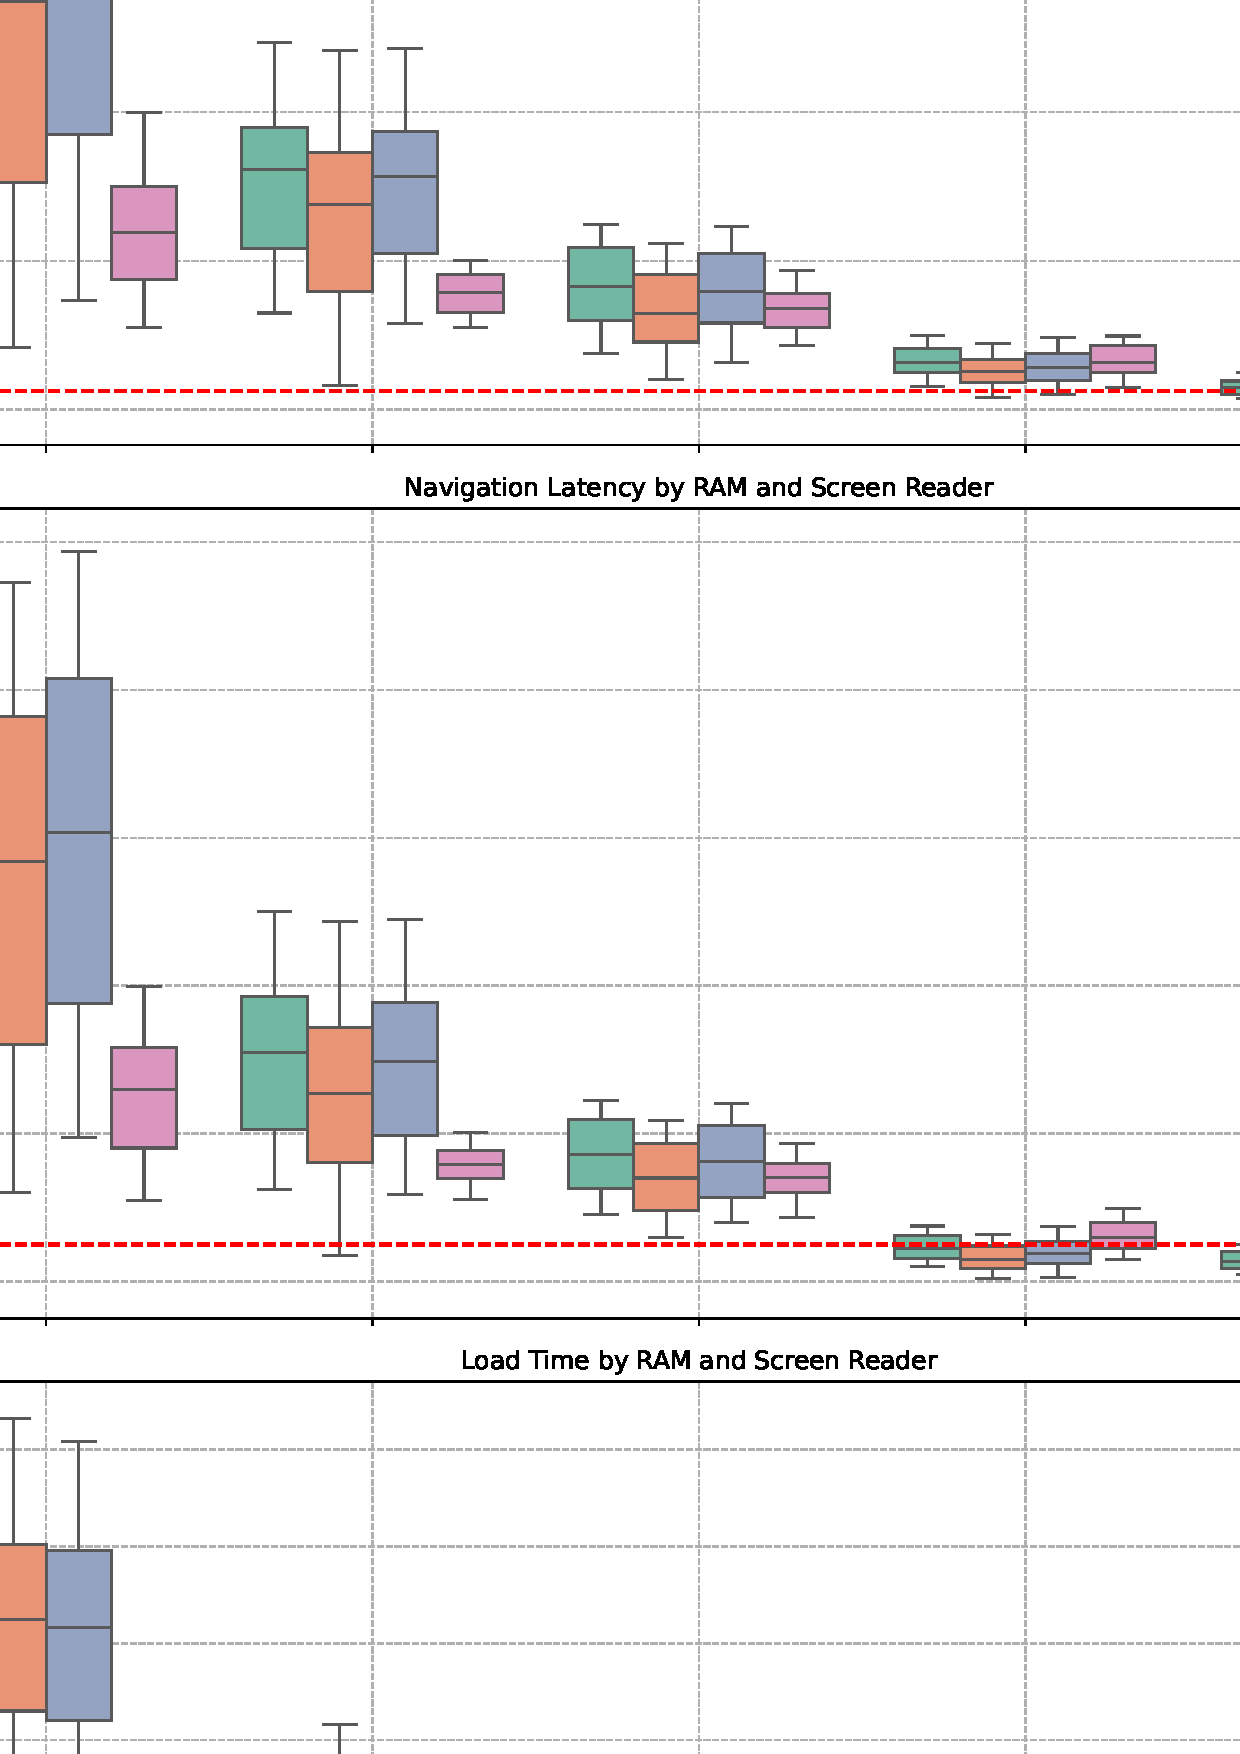
\includegraphics[keepaspectratio,width=0.9\linewidth,height=0.9\textheight]{composite_latency}}
	\caption{Composite latency comparison (keystroke echo, navigation command, load time)}
	\label{fig:figure4}
\end{figure}

\subsubsection*{Consolidated Latency Performance Summary}
\scriptsize
\begin{longtblr}[
		caption = {Consolidated Latency Summary (Rounded Intervals): NVDA nears parity earlier; others need higher RAM for partial convergence.},
		label = {tab:chap1-consolidated-latency},
		entry = {Latency Summary},
		note = {Intervals simplified; qualitative notes unchanged.}
	]{width=\textwidth, colspec={X[l] X[l] X[r] X[r] X[r] X[l]}, rowhead=1, row{1} = {font=\bfseries}, hlines, stretch=1.5}

	Domain                        & Engine (Representative)     & Low RAM (16GB)       & Transitional (24/32GB) & High (64GB)        & Equity / Variability Note                                                    \\

	Startup (Load)                & NVDA                        & 11–14 s              & 9–11 s                 & 8–10 s             & Near <10 s threshold by 24–32GB; low variance                                \\
	Startup (Load)                & JAWS / Narrator / SuperNova & 50–70 s              & 45–55 s                & 40–50 s            & 4–5× slower than spontaneous threshold; long-tail stalls persist             \\
	Keystroke Echo                & NVDA                        & 130–160 ms           & 110–140 ms             & 100–120 ms         & Early approach to sub-150 ms fluidity; stable rhythm                         \\
	Keystroke Echo                & JAWS / Narrator             & 200–320 ms           & 160–250 ms             & 140–210 ms         & High dispersion; right-tail spikes disrupt rhythm                            \\
	Keystroke Echo                & SuperNova                   & 180–280 ms           & 150–230 ms             & 130–190 ms         & Intermediate; variance still elevated                                        \\
	Navigation Commands 		  & NVDA                        & 140–190 ms           & 125–160 ms             & 115–140 ms         & Only engine consistently near sub-150 ms boundary                            \\
	Navigation Commands 		  & JAWS / Narrator             & 230–360 ms           & 180–300 ms             & 160–250 ms         & Large IQR; unpredictability hinders scanning                                 \\
	Navigation Commands 		  & SuperNova                   & 210–320 ms           & 170–260 ms             & 150–230 ms         & Slightly faster than JAWS/Narrator; skew remains                             \\
	Composite Equity Gap          & NVDA                        & Key 5–6×; Nav 7–9×   & Key 4–5×; Nav 6–7×     & Key 4×; Nav 5–6×   & Lowest multiplicative gaps; diminishing returns absent architecture gains    \\
	Composite Equity Gap          & Other Engines               & Key 8–12×; Nav 9–14× & Key 6–10×; Nav 7–11×   & Key 5–8×; Nav 6–9× & RAM lowers means but variability sustains inequity; choice still constrained \\
\end{longtblr}
\normalsize

\noindent\textbf{Consolidated Interpretation.} This summary underscores three equity dynamics: (1) \emph{Architecture First}: Only one engine converts RAM into both lower means and suppressed variance early; others remain volatility-prone. (2) \emph{Variance as Barrier}: Even when mean latencies shrink, wide IQR / right tails sustain cognitive interruption penalties—equity cannot be judged on averages alone. (3) \emph{Choice vs. Coercion}: At sub-32GB tiers, only a single engine approaches functional fluidity, effectively coercing adoption; genuine choice emerges only once RAM reaches 32–64GB \emph{and} even then architectural gaps impose residual multiplicative disadvantages, justifying continued performance engineering advocacy.

Between the 32GB near-parity tier and the fully equity-compliant 64GB tier, dispersion (IQR, tail spikes) across major \gidx{screenreader}{screen reader} engines contracts enough that no single product’s latency profile monopolizes viability. This convergence transforms hardware provisioning from a de facto engine mandate into authentic user choice: NVDA’s strength in low-variance structural \gidx{navigation}{navigation}, JAWS’s broader legacy/enterprise application scripts, SuperNova’s integrated \gidx{magnification}{magnification} and visual enhancement stack, and Narrator’s frictionless OS onboarding can each be leveraged without imposing a disproportionate latency tax. Policy significance: specifying 32–64GB \gidx{ram}{RAM} protects pedagogical flexibility—students and disability services can align tool selection with task demands (STEM notation, rich web apps, rapid reading, low-vision hybrid use) rather than trading functional features for basic responsiveness. Sustaining this choice space is an equity outcome in itself, preventing a “single-performer lock-in” that would otherwise emerge at lower memory tiers where latency differentials coerce migration.

For detailed statistical breakdown see \ref{chap:computationappendix}.

\section{Assistive Technology-Capable Laptop Hardware Matrix}\label{sec:assistive-laptop-matrix}

\footnotesize
\begin{longtblr}[
		caption = {Comprehensive Laptop Specifications for Assistive Technology Workloads},
		label = {tab:assistive-laptops},
		note = {Representative 2024–2025 models spanning Intel Core Ultra (Lunar Lake / Meteor Lake), AMD Ryzen AI (XDNA), and Snapdragon X platforms. Focused on configurations suitable for concurrent screen reader, \gidx{magnification}{magnification}, \gls{ocr}, AI captioning, and real-time transcription tasks. NPU TOPS values are vendor-published peak INT8 figures (verify sustained performance under thermal constraints). Price bands reflect typical US MSRP at time of drafting; institutional and education pricing may reduce acquisition cost.}
	]{
		colspec = {X[1,l] X[1.2,l] X[0.8,c] X[0.8,c] X[1,c] X[1,c] X[0.8,c] X[0.8,c]},
		rowhead = 1,
		row{1} = {font=\bfseries},
		hlines,
		stretch = 1.5
	}
	Model                                   & \gidx{processor}{Processor}   & NPU TOPS & RAM               & Display                   \         & Graphics            & Storage          & Est. Price    \\
	% Intel Core Ultra Series 2 (Lunar Lake) - Dell
	Dell XPS 13 Plus (2025)                 & Intel Core Ultra 7 258V       & 48       & 32GB LPDDR5X-8533 & 13.4" 3K+ OLED Touch (3200×2000)   & Intel Arc 140V      & 1TB PCIe 4.0 SSD & \$1,899–2,299 \\
	Dell XPS 14 (2025)                      & Intel Core Ultra 7 258V       & 48       & 32GB LPDDR5X-8533 & 14.5" 3K+ OLED Touch (3200×2000)   & Intel Arc 140V      & 1TB PCIe 4.0 SSD & \$2,199–2,599 \\
	Dell XPS 16 (2025)                      & Intel Core Ultra 9 268V       & 48       & 32GB LPDDR5X-8533 & 16" 4K+ OLED Touch (3840×2400)     & Intel Arc 140V      & 1TB PCIe 4.0 SSD & \$2,499–2,999 \\
	Dell XPS 16 (2025)                      & Intel Core Ultra 9 268V       & 48       & 64GB LPDDR5X-8533 & 16" 4K+ OLED Touch (3840×2400)     & Intel Arc 140V      & 2TB PCIe 4.0 SSD & \$3,199–3,699 \\
	% Intel Core Ultra Series 1 (Meteor Lake) - Dell
	Dell XPS 14 (2024)                      & Intel Core Ultra 7 155H       & 10       & 32GB LPDDR5X-7467 & 14.5" 3.2K+ OLED Touch (3200×2000) & Arc + RTX 4050      & 1TB PCIe 4.0 SSD & \$2,299–2,799 \\
	Dell XPS 14 (2024)                      & Intel Core Ultra 9 185H       & 10       & 64GB LPDDR5X-7467 & 14.5" 3.2K+ OLED Touch (3200×2000) & Arc + RTX 4060      & 2TB PCIe 4.0 SSD & \$3,499–3,999 \\
	Dell XPS 15 (2024)                      & Intel Core Ultra 7 155H       & 10       & 32GB DDR5-5600    & 15.6" 3.5K OLED (3456×2160)        & Arc + RTX 4050      & 1TB PCIe 4.0 SSD & \$2,399–2,899 \\
	Dell XPS 15 (2024)                      & Intel Core Ultra 9 185H       & 10       & 64GB DDR5-5600    & 15.6" 3.5K OLED (3456×2160)        & Arc + RTX 4060      & 2TB PCIe 4.0 SSD & \$3,599–4,099 \\
	Dell XPS 17 (2024)                      & Intel Core Ultra 9 185H       & 10       & 32GB DDR5-5600    & 17" 4K+ (3840×2400)                & Arc + RTX 4070      & 1TB PCIe 4.0 SSD & \$2,799–3,299 \\
	Dell XPS 17 (2024)                      & Intel Core Ultra 9 185H       & 10       & 64GB DDR5-5600    & 17" 4K+ (3840×2400)                & Arc + RTX 4080      & 2TB PCIe 4.0 SSD & \$4,199–4,699 \\
	% Dell Precision Workstations
	Dell Precision 5490                     & Intel Core Ultra 7 165H       & 10       & 32GB DDR5-5600    & 14" 2.5K (2560×1600)               & NVIDIA RTX 2000 Ada & 1TB PCIe 4.0 SSD & \$3,199–3,699 \\
	Dell Precision 5490                     & Intel Core Ultra 9 185H       & 10       & 64GB DDR5-5600    & 14" 2.5K (2560×1600)               & NVIDIA RTX 3000 Ada & 2TB PCIe 4.0 SSD & \$4,499–4,999 \\
	Dell Precision 5690                     & Intel Core Ultra 9 185H       & 10       & 32GB DDR5-5600    & 16" 4K+ OLED Touch (3840×2400)     & NVIDIA RTX 3000 Ada & 1TB PCIe 4.0 SSD & \$3,699–4,199 \\
	Dell Precision 5690                     & Intel Core Ultra 9 185H       & 10       & 64GB DDR5-5600    & 16" 4K+ OLED Touch (3840×2400)     & NVIDIA RTX 4000 Ada & 2TB PCIe 4.0 SSD & \$4,199–4,999 \\
	Dell Precision 7780                     & Intel Core i9-13980HX          & 0        & 32GB DDR5-5600    & 17.3" 4K (3840×2160)               & NVIDIA RTX 4000 Ada & 1TB PCIe 4.0 SSD & \$4,299–4,799 \\
	Dell Precision 7780                     & Intel Core i9-13980HX          & 0        & 64GB DDR5-5600    & 17.3" 4K (3840×2160)               & NVIDIA RTX 5000 Ada & 2TB PCIe 4.0 SSD & \$5,999–6,499 \\
	% Dell Pro Series
	Dell Pro 13 Premium                     & Intel Core Ultra 5 236V       & 48       & 32GB LPDDR5X-8533 & 13" FHD+ (1920×1200)               & Intel Arc Graphics  & 512GB/1TB SSD    & \$1,299–1,699 \\
	Dell Pro 14 Premium                     & Intel Core Ultra 5 236V       & 48       & 32GB LPDDR5X-8533 & 14" FHD+ (1920×1200)               & Intel Arc Graphics  & 512GB/1TB SSD    & \$1,399–1,799 \\
	Dell Pro 14 Plus                        & Intel Core Ultra 7 258V       & 48       & 32GB LPDDR5X-8533 & 14" QHD+ Touch (2560×1600)         & Intel Arc 140V      & 1TB PCIe 4.0 SSD & \$1,699–2,199 \\
	Dell Pro 16 Plus (Intel)                & Intel Core Ultra 7 258V       & 48       & 32GB DDR5-5600    & 16" FHD+ (1920×1200)               & Intel Arc 140V      & 1TB PCIe 4.0 SSD & \$1,899–2,399 \\
	Dell Pro 16 Plus (AMD)                  & AMD Ryzen AI 9 PRO 365        & 50       & 32GB DDR5-5600    & 16" FHD+ (1920×1200)               & Radeon 880M         & 1TB PCIe 4.0 SSD & \$1,799–2,299 \\
	% Dell Pro Max Series
	Dell Pro Max 14                         & Intel Core Ultra 5 235H       & 10       & 32GB DDR5-5600    & 14" FHD+ (1920×1200)               & Intel Arc Graphics  & 1TB PCIe 4.0 SSD & \$2,199–2,699 \\
	Dell Pro Max 14                         & Intel Core Ultra 9 285H       & 10       & 64GB DDR5-6400    & 14" 2.5K (2560×1600)               & Intel Arc Graphics  & 2TB PCIe 4.0 SSD & \$3,199–3,699 \\
	Dell Pro Max 16                         & Intel Core Ultra 9 285H       & 10       & 32GB DDR5-5600    & 16" FHD+ (1920×1200)               & Intel Arc Graphics  & 1TB PCIe 4.0 SSD & \$2,699–3,199 \\
	Dell Pro Max 16                         & Intel Core Ultra 9 285H       & 10       & 64GB DDR5-6400    & 16" 4K (3840×2400)                 & Intel Arc Graphics  & 2TB PCIe 4.0 SSD & \$3,699–4,199 \\
	Dell Pro Max 16 Plus                    & Intel Core Ultra 9 285H       & 10       & 32GB DDR5-5600    & 16" 4K (3840×2400)                 & NVIDIA RTX 2000 Ada & 1TB PCIe 4.0 SSD & \$3,199–3,699 \\
	Dell Pro Max 16 Plus                    & Intel Core Ultra 9 285H       & 10       & 64GB DDR5-6400    & 16" 4K (3840×2400)                 & NVIDIA RTX 3000 Ada & 2TB PCIe 4.0 SSD & \$4,199–4,699 \\
	Dell Pro Max 16 Premium                 & Intel Core Ultra 9 285H       & 10       & 32GB DDR5-5600    & 16" 4K OLED (3840×2400)            & NVIDIA RTX 3000 Ada & 1TB PCIe 4.0 SSD & \$3,999–4,499 \\
	Dell Pro Max 16 Premium                 & Intel Core Ultra 9 285H       & 10       & 64GB DDR5-6400    & 16" 4K OLED (3840×2400)            & NVIDIA RTX 4000 Ada & 2TB PCIe 4.0 SSD & \$4,999–5,499 \\
	% HP OmniBook Series
	HP OmniBook X 14 (Snapdragon)          & Snapdragon X Elite X1E-78-100 & 45       & 32GB LPDDR5X-8448 & 14" 2.2K IPS Touch (2240×1400)     & Adreno GPU          & 1TB PCIe 4.0 SSD & \$1,699–2,099 \\
	HP OmniBook X 14 (Snapdragon)          & Snapdragon X Plus X1P-64-100  & 45       & 16GB LPDDR5X-8448 & 14" 2.2K IPS Touch (2240×1400)     & Adreno GPU          & 512GB SSD        & \$1,199–1,499 \\
	HP OmniBook Ultra 14                    & AMD Ryzen AI 9 365             & 50       & 32GB LPDDR5X-7500 & 14" 2.2K OLED Touch (2240×1400)    & Radeon 880M         & 1TB PCIe 4.0 SSD & \$1,899–2,299 \\
	HP OmniBook Ultra 14                    & AMD Ryzen AI 9 HX 375          & 50       & 32GB LPDDR5X-7500 & 14" 2.2K OLED Touch (2240×1400)    & Radeon 890M         & 2TB PCIe 4.0 SSD & \$2,199–2,599 \\
	HP OmniBook Ultra Flip 14               & AMD Ryzen AI 9 HX 370          & 50       & 32GB LPDDR5X-7500 & 14" 2.8K OLED Touch (2880×1800)    & Radeon 890M         & 1TB PCIe 4.0 SSD & \$1,899–2,299 \\
	HP OmniBook 5 14                        & AMD Ryzen AI 7 340             & 50       & 32GB LPDDR5X-7500 & 14" 2K OLED (2240×1400)            & Radeon 760M         & 1TB PCIe 4.0 SSD & \$1,599–1,999 \\
	HP OmniBook 5 16                        & AMD Ryzen AI 7 340             & 50       & 32GB LPDDR5X-7500 & 16" 2K (2240×1400)                 & Radeon 760M         & 1TB PCIe 4.0 SSD & \$1,699–2,099 \\
	% HP EliteBook Series
	HP EliteBook 840 G12                    & Intel Core Ultra 7 258V       & 48       & 32GB DDR5-5600    & 14" FHD+ IPS / 2.8K OLED           & Intel Arc 140V      & 1TB PCIe 4.0 SSD & \$1,999–2,499 \\
	HP EliteBook 840 G12                    & Intel Core Ultra 9 268V       & 48       & 64GB DDR5-5600    & 14" 2.8K OLED                      & Intel Arc 140V      & 2TB PCIe 4.0 SSD & \$2,899–3,299 \\
	HP EliteBook 860 G12                    & Intel Core Ultra 7 258V       & 48       & 32GB DDR5-5600    & 16" WUXGA / 4K OLED                & Intel Arc 140V      & 1TB PCIe 4.0 SSD & \$2,199–2,699 \\
	HP EliteBook 860 G12                    & Intel Core Ultra 9 268V       & 48       & 64GB DDR5-5600    & 16" 4K OLED                        & Intel Arc 140V      & 2TB PCIe 4.0 SSD & \$3,199–3,699 \\
	HP EliteBook Ultra 14                   & AMD Ryzen AI 9 HX 375          & 50       & 32GB LPDDR5X-7500 & 14" 2.8K OLED                      & Radeon 890M         & 1TB PCIe 4.0 SSD & \$2,299–2,799 \\
	HP EliteBook Ultra 14                   & AMD Ryzen AI 9 HX 375          & 50       & 64GB LPDDR5X-7500 & 14" 2.8K OLED                      & Radeon 890M         & 2TB PCIe 4.0 SSD & \$3,199–3,699 \\
	% Lenovo ThinkPad X1 Series
	Lenovo ThinkPad X1 Carbon Gen 13        & Intel Core Ultra 7 268V       & 48       & 32GB LPDDR5X-8533 & 14" WUXGA IPS / 2.8K OLED          & Intel Arc 140V      & 1TB PCIe 4.0 SSD & \$2,199–2,699 \\
	Lenovo ThinkPad X1 Carbon Gen 13        & Intel Core Ultra 9 288V       & 48       & 64GB LPDDR5X-8533 & 14" 2.8K OLED                      & Intel Arc 140V      & 2TB PCIe 5.0 SSD & \$3,299–3,799 \\
	Lenovo ThinkPad X1 2-in-1 Gen 10        & Intel Core Ultra 7 258V       & 48       & 32GB LPDDR5X-8533 & 14" 2.8K OLED Touch 120Hz          & Intel Arc 140V      & 1TB PCIe 5.0 SSD & \$2,199–2,699 \\
	Lenovo ThinkPad X1 2-in-1 Gen 10        & Intel Core Ultra 9 288V       & 48       & 64GB LPDDR5X-8533 & 14" 2.8K OLED Touch 120Hz          & Intel Arc 140V      & 2TB PCIe 5.0 SSD & \$3,399–3,899 \\
	Lenovo ThinkPad X9 15 Aura Edition       & Intel Core Ultra 7 258V       & 48       & 32GB LPDDR5X-8533 & 15" 2.8K OLED (2880×1800)          & Intel Arc 140V      & 1TB PCIe 5.0 SSD & \$2,399–2,899 \\
	Lenovo ThinkPad X9 15 Aura Edition       & Intel Core Ultra 9 288V       & 48       & 64GB LPDDR5X-8533 & 15" 2.8K OLED (2880×1800)          & Intel Arc 140V      & 2TB PCIe 5.0 SSD & \$3,499–3,999 \\
	% Lenovo ThinkPad T Series
	Lenovo ThinkPad T14s Gen 6 (Intel)      & Intel Core Ultra 7 258V       & 48       & 32GB LPDDR5X-8533 & 14" WUXGA / 2.8K OLED              & Intel Arc 140V      & 1TB PCIe 4.0 SSD & \$1,899–2,399 \\
	Lenovo ThinkPad T14s Gen 6 (Intel)      & Intel Core Ultra 9 268V       & 48       & 64GB LPDDR5X-8533 & 14" 2.8K OLED                      & Intel Arc 140V      & 2TB PCIe 4.0 SSD & \$2,999–3,499 \\
	Lenovo ThinkPad T14s Gen 6 (Snapdragon) & Snapdragon X Plus X1P-64-100  & 45       & 32GB LPDDR5X-8448 & 14" WUXGA / 2.8K OLED              & Adreno GPU          & 1TB PCIe 4.0 SSD & \$1,899–2,299 \\
	Lenovo ThinkPad T14s Gen 6 (AMD)        & AMD Ryzen AI 9 HX 370          & 50       & 32GB LPDDR5X-7500 & 14" 2.8K OLED                      & Radeon 890M         & 1TB PCIe 4.0 SSD & \$1,999–2,499 \\
	Lenovo ThinkPad T14s Gen 6 (AMD)        & AMD Ryzen AI 9 HX 370          & 50       & 64GB LPDDR5X-7500 & 14" 2.8K OLED                      & Radeon 890M         & 2TB PCIe 4.0 SSD & \$2,899–3,399 \\
	Lenovo ThinkPad T14 Gen 6               & Intel Core Ultra 7 155U       & 10       & 32GB DDR5-5600    & 14" WUXGA IPS (1920×1200)          & Intel Arc Graphics  & 1TB PCIe 4.0 SSD & \$1,599–2,099 \\
	Lenovo ThinkPad T14 Gen 6               & Intel Core Ultra 7 165H       & 10       & 64GB DDR5-5600    & 14" 2.8K OLED                      & Intel Arc Graphics  & 2TB PCIe 4.0 SSD & \$2,699–3,199 \\
	% Lenovo ThinkPad P Series
	Lenovo ThinkPad P1 Gen 7                & Intel Core Ultra 9 185H       & 10       & 32GB DDR5-5600    & 16" 4K OLED (3840×2400)            & NVIDIA RTX 3000 Ada & 1TB PCIe 4.0 SSD & \$3,799–4,299 \\
	Lenovo ThinkPad P1 Gen 7                & Intel Core Ultra 9 185H       & 10       & 64GB DDR5-5600    & 16" 4K OLED (3840×2400)            & NVIDIA RTX 4080     & 2TB PCIe 4.0 SSD & \$4,299–5,199 \\
	Lenovo ThinkPad P16s Gen 3              & Intel Core Ultra 7 165H       & 10       & 32GB DDR5-5600    & 16" WUXGA IPS (1920×1200)          & NVIDIA RTX 2000 Ada & 1TB PCIe 4.0 SSD & \$2,899–3,399 \\
	Lenovo ThinkPad P16s Gen 3              & Intel Core Ultra 9 185H       & 10       & 64GB DDR5-5600    & 16" 4K (3840×2400)                 & NVIDIA RTX 3000 Ada & 2TB PCIe 4.0 SSD & \$4,199–4,699 \\
	% Lenovo ThinkBook Series
	Lenovo ThinkBook 16 Gen 7               & Intel Core Ultra 7 155U       & 10       & 32GB DDR5-5600    & 16" WUXGA IPS (1920×1200)          & Intel Arc Graphics  & 1TB PCIe 4.0 SSD & \$1,599–1,999 \\
	Lenovo ThinkBook 16 Gen 7               & Intel Core Ultra 9 185H       & 10       & 64GB DDR5-5600    & 16" 2.5K (2560×1600)               & Intel Arc Graphics  & 2TB PCIe 4.0 SSD & \$2,499–2,999 \\
	Lenovo ThinkBook Plus Gen 6 Rollable    & Intel Core Ultra 7 258V       & 48       & 32GB LPDDR5X-8533 & 14" Rollable OLED (2048×1536)      & Intel Arc 140V      & 1TB PCIe 5.0 SSD & \$3,999–4,499 \\
	Lenovo IdeaPad Pro 5 14                 & AMD Ryzen AI 7 PRO 360         & 50       & 32GB LPDDR5X-7500 & 14" 2.8K OLED (2880×1800)          & Radeon 880M         & 1TB PCIe 4.0 SSD & \$1,599–1,999 \\
	Lenovo IdeaPad Pro 5 16                 & AMD Ryzen AI 9 HX 370          & 50       & 32GB LPDDR5X-7500 & 16" 2.5K OLED (2560×1600)          & Radeon 890M         & 1TB PCIe 4.0 SSD & \$1,799–2,199 \\
	% ASUS ZenBook Series
	ASUS Zenbook S 13 OLED                  & Intel Core Ultra 7 258V       & 48       & 32GB LPDDR5X-8533 & 13.3" 2.8K OLED (2880×1800)        & Intel Arc 140V      & 1TB PCIe 4.0 SSD & \$1,799–2,199 \\
	ASUS Zenbook S 14 OLED                  & Intel Core Ultra 9 268V       & 48       & 32GB LPDDR5X-8533 & 14" 2.8K OLED (2880×1800)          & Intel Arc 140V      & 1TB PCIe 4.0 SSD & \$1,999–2,399 \\
	ASUS Zenbook 14 OLED (Snapdragon)       & Snapdragon X Elite X1E-78-100 & 45       & 32GB LPDDR5X-8448 & 14" 2.8K OLED (2880×1800)          & Adreno GPU          & 1TB PCIe 4.0 SSD & \$1,599–1,999 \\
	ASUS Zenbook 14 OLED (AMD)              & AMD Ryzen AI 9 HX 370          & 50       & 32GB LPDDR5X-7500 & 14" 2.8K OLED (2880×1800)          & Radeon 890M         & 1TB PCIe 4.0 SSD & \$1,699–2,099 \\
	ASUS Zenbook Pro 16X OLED               & Intel Core Ultra 9 185H       & 10       & 32GB DDR5-5600    & 16" 4K+ OLED Touch (3200×2000)     & NVIDIA RTX 4060     & 1TB PCIe 4.0 SSD & \$2,699–3,199 \\
	ASUS Zenbook Pro 16X OLED               & Intel Core Ultra 9 185H       & 10       & 64GB DDR5-5600    & 16" 4K+ OLED Touch (3200×2000)     & NVIDIA RTX 4070     & 2TB PCIe 4.0 SSD & \$3,799–4,299 \\
	% ASUS Vivobook Series
	ASUS Vivobook S 14 (Intel)              & Intel Core Ultra 7 258V       & 48       & 32GB LPDDR5X-8533 & 14" 2.8K OLED (2880×1800)          & Intel Arc 140V      & 1TB PCIe 4.0 SSD & \$1,699–2,099 \\
	ASUS Vivobook S 14 (AMD)                & AMD Ryzen AI 9 HX 370          & 50       & 32GB LPDDR5X-7500 & 14" 2.8K OLED (2880×1800)          & Radeon 890M         & 1TB PCIe 4.0 SSD & \$1,699–2,099 \\
	ASUS Vivobook S 15 (Snapdragon)         & Snapdragon X Elite X1E-78-100 & 45       & 32GB LPDDR5X-8448 & 15.6" 3K OLED (2880×1620)          & Adreno GPU          & 1TB PCIe 4.0 SSD & \$1,799–2,199 \\
	ASUS Vivobook Pro 15 OLED               & AMD Ryzen AI 9 HX 370          & 50       & 32GB DDR5-5600    & 15.6" 2.8K OLED (2880×1620)        & Radeon 890M         & 1TB PCIe 4.0 SSD & \$1,899–2,299 \\
	% ASUS ROG Series (Gaming/Workstation)
	ASUS ROG Zephyrus G14 (2024 Intel)      & Intel Core Ultra 9 185H       & 10       & 32GB DDR5-5600    & 14" 2.5K OLED 120Hz (2560×1600)    & Arc + RTX 4060      & 1TB PCIe 4.0 SSD & \$2,199–2,699 \\
	ASUS ROG Zephyrus G14 (2024 AMD)        & AMD Ryzen AI 9 HX 370          & 50       & 32GB DDR5-5600    & 14" 2.5K OLED 120Hz (2560×1600)    & RTX 4070            & 1TB PCIe 4.0 SSD & \$2,299–2,799 \\
	ASUS ROG Zephyrus G16 (2024)            & Intel Core Ultra 9 185H       & 10       & 32GB DDR5-5600    & 16" 2.5K OLED 240Hz (2560×1600)    & RTX 4080            & 1TB PCIe 4.0 SSD & \$2,999–3,499 \\
	ASUS ROG Zephyrus G16 (2024)            & Intel Core Ultra 9 185H       & 10       & 64GB DDR5-5600    & 16" 2.5K OLED 240Hz (2560×1600)    & RTX 4090            & 2TB PCIe 4.0 SSD & \$4,199–4,699 \\
	% ASUS ProArt Series
	ASUS ProArt Studiobook 16 OLED          & Intel Core Ultra 9 185H       & 10       & 32GB DDR5-5600    & 16" 4K OLED (3840×2400)            & NVIDIA RTX 4070     & 1TB PCIe 4.0 SSD & \$3,199–3,699 \\
	ASUS ProArt Studiobook 16 OLED          & Intel Core Ultra 9 185H       & 10       & 64GB DDR5-5600    & 16" 4K OLED (3840×2400)            & NVIDIA RTX 4080     & 2TB PCIe 4.0 SSD & \$4,499–4,999 \\
	% Framework Laptop Series
	Framework Laptop 13 (Intel)             & Intel Core Ultra 7 258V       & 48       & 32GB DDR5-5600    & 13.5" 2256×1504 IPS (3:2)          & Intel Arc 140V      & 1TB PCIe 4.0 SSD & \$1,799–2,199 \\
	Framework Laptop 13 (Intel)             & Intel Core Ultra 9 268V       & 48       & 64GB DDR5-5600    & 13.5" 2256×1504 IPS (3:2)          & Intel Arc 140V      & 2TB PCIe 4.0 SSD & \$2,699–3,199 \\
	Framework Laptop 13 (AMD)               & AMD Ryzen AI 7 8840U          & 16       & 32GB DDR5-5600    & 13.5" 2256×1504 IPS (3:2)          & Radeon 780M         & 1TB PCIe 4.0 SSD & \$1,799–2,199 \\
	Framework Laptop 13 (AMD)               & AMD Ryzen AI 9 8945H          & 16       & 64GB DDR5-5600    & 13.5" 2256×1504 IPS (3:2)          & Radeon 780M         & 2TB PCIe 4.0 SSD & \$2,599–3,099 \\
	Framework Laptop 16                     & AMD Ryzen 9 7940HS            & 0        & 32GB DDR5-5600    & 16" 2560×1600 IPS (16:10)          & Radeon 780M         & 1TB PCIe 4.0 SSD & \$2,199–2,699 \\
	Framework Laptop 16                     & AMD Ryzen 9 7940HS            & 0        & 64GB DDR5-5600    & 16" 2560×1600 IPS (16:10)          & RX 7700S dGPU       & 2TB PCIe 4.0 SSD & \$3,299–3,799 \\
	% Acer Swift Series
	Acer Swift 14 AI (Intel)                & Intel Core Ultra 7 258V       & 48       & 32GB LPDDR5X-8533 & 14" 2.8K OLED (2880×1800)          & Intel Arc 140V      & 1TB PCIe 4.0 SSD & \$1,599–1,999 \\
	Acer Swift 16 AI                        & AMD Ryzen AI 9 HX 370          & 50       & 32GB LPDDR5X-7500 & 16" 2.5K OLED (2560×1600)          & Radeon 890M         & 1TB PCIe 4.0 SSD & \$1,799–2,199 \\
	Acer Swift X 14 (2025)                  & Intel Core Ultra 7 258V       & 48       & 32GB LPDDR5X-8533 & 14" 2.8K OLED (2880×1800)          & NVIDIA RTX 4050     & 1TB PCIe 4.0 SSD & \$1,899–2,399 \\
	% Acer Predator Series
	Acer Predator Helios Neo 16             & Intel Core Ultra 9 185H       & 10       & 32GB DDR5-5600    & 16" 2.5K IPS 165Hz (2560×1600)     & NVIDIA RTX 4070     & 1TB PCIe 4.0 SSD & \$2,199–2,699 \\
	Acer Predator Helios Neo 16             & Intel Core Ultra 9 185H       & 10       & 64GB DDR5-5600    & 16" 2.5K IPS 165Hz (2560×1600)     & NVIDIA RTX 4080     & 2TB PCIe 4.0 SSD & \$3,399–3,899 \\
	% Acer ConceptD Series
	Acer ConceptD 7 Ezel                    & Intel Core Ultra 9 185H       & 10       & 32GB DDR5-5600    & 15.6" 4K OLED Touch (3840×2160)    & NVIDIA RTX 4070     & 1TB PCIe 4.0 SSD & \$3,499–3,999 \\
	Acer ConceptD 7 Ezel                    & Intel Core Ultra 9 185H       & 10       & 64GB DDR5-5600    & 15.6" 4K OLED Touch (3840×2160)    & NVIDIA RTX 4080     & 2TB PCIe 4.0 SSD & \$4,799–5,299 \\
	% Microsoft Surface Series
	Microsoft Surface Laptop 7 (Intel)      & Intel Core Ultra 7 268V       & 48       & 32GB LPDDR5X-8533 & 13.8" PixelSense (2304×1536)       & Intel Arc 140V      & 1TB PCIe 4.0 SSD & \$2,199–2,599 \\
	Microsoft Surface Laptop 7 (Intel)      & Intel Core Ultra 9 288V       & 48       & 64GB LPDDR5X-8533 & 15" PixelSense (2496×1664)         & Intel Arc 140V      & 2TB PCIe 4.0 SSD & \$3,199–3,699 \\
	Microsoft Surface Laptop 7 (Snapdragon) & Snapdragon X Elite X1E-80-100 & 45       & 32GB LPDDR5X-8448 & 13.8" PixelSense (2304×1536)       & Adreno GPU          & 1TB PCIe 4.0 SSD & \$1,999–2,399 \\
	Microsoft Surface Laptop Studio 3       & Intel Core Ultra 9 185H       & 10       & 32GB DDR5-5600    & 14.4" PixelSense Touch (2400×1600) & NVIDIA RTX 4060     & 1TB PCIe 4.0 SSD & \$3,199–3,699 \\
	Microsoft Surface Laptop Studio 3       & Intel Core Ultra 9 185H       & 10       & 64GB DDR5-5600    & 14.4" PixelSense Touch (2400×1600) & NVIDIA RTX 4070     & 2TB PCIe 4.0 SSD & \$4,499–4,999 \\
	Microsoft Surface Book 5                & Intel Core Ultra 9 268V       & 48       & 32GB LPDDR5X-8533 & 15" PixelSense Touch (3240×2160)   & NVIDIA RTX 4050     & 1TB PCIe 5.0 SSD & \$3,999–4,499 \\
	Microsoft Surface Book 5                & Intel Core Ultra 9 268V       & 48       & 64GB LPDDR5X-8533 & 15" PixelSense Touch (3240×2160)   & NVIDIA RTX 4070     & 2TB PCIe 5.0 SSD & \$5,199–5,699 \\
	% Samsung Galaxy Book Series
	Samsung Galaxy Book4 Edge 14            & Snapdragon X Elite X1E-80-100 & 45       & 32GB LPDDR5X-8448 & 14" FHD+ AMOLED Touch (1920×1200)  & Adreno GPU          & 1TB PCIe 4.0 SSD & \$1,699–2,099 \\
	Samsung Galaxy Book4 Edge 16            & Snapdragon X Elite X1E-84-100 & 45       & 32GB LPDDR5X-8448 & 16" 2.8K AMOLED Touch (2880×1800)  & Adreno GPU          & 1TB PCIe 4.0 SSD & \$1,899–2,299 \\
	Samsung Galaxy Book4 Pro 14             & Intel Core Ultra 7 155H       & 10       & 32GB LPDDR5X-7467 & 14" 2.8K AMOLED Touch (2880×1800)  & Intel Arc Graphics  & 1TB PCIe 4.0 SSD & \$1,799–2,199 \\
	Samsung Galaxy Book4 Pro 16             & Intel Core Ultra 9 185H       & 10       & 32GB LPDDR5X-7467 & 16" 2.8K AMOLED Touch (2880×1800)  & NVIDIA RTX 4050     & 1TB PCIe 4.0 SSD & \$2,199–2,699 \\
	Samsung Galaxy Book4 Pro 16             & Intel Core Ultra 9 185H       & 10       & 64GB LPDDR5X-7467 & 16" 2.8K AMOLED Touch (2880×1800)  & NVIDIA RTX 4060     & 2TB PCIe 4.0 SSD & \$3,199–3,699 \\
	% Razer Blade Series
	Razer Blade 14 (2025)                   & AMD Ryzen AI 9 HX 370          & 50       & 32GB DDR5-5600    & 14" 2.5K 165Hz (2560×1600)         & NVIDIA RTX 4070     & 1TB PCIe 4.0 SSD & \$2,699–3,199 \\
	Razer Blade 16 (2025)                   & Intel Core Ultra 9 185H       & 10       & 32GB DDR5-5600    & 16" 4K 120Hz (3840×2400)           & NVIDIA RTX 4080     & 1TB PCIe 4.0 SSD & \$3,299–3,799 \\
	Razer Blade 16 (2025)                   & Intel Core Ultra 9 185H       & 10       & 64GB DDR5-5600    & 16" 4K 120Hz (3840×2400)           & NVIDIA RTX 4090     & 2TB PCIe 4.0 SSD & \$4,699–5,199 \\
	% MSI Prestige Series
	MSI Prestige 13 AI+ Evo                 & Intel Core Ultra 7 258V       & 48       & 32GB LPDDR5X-8533 & 13.3" 2.8K OLED (2880×1800)        & Intel Arc 140V      & 1TB PCIe 4.0 SSD & \$1,699–2,099 \\
	MSI Prestige 16 AI Studio               & Intel Core Ultra 9 185H       & 10       & 32GB DDR5-5600    & 16" 4K Mini LED (3840×2400)        & NVIDIA RTX 4070     & 1TB PCIe 4.0 SSD & \$2,799–3,299 \\
	MSI Prestige 16 AI Studio               & Intel Core Ultra 9 185H       & 10       & 64GB DDR5-5600    & 16" 4K Mini LED (3840×2400)        & NVIDIA RTX 4080     & 2TB PCIe 4.0 SSD & \$3,899–4,399 \\
	% Gigabyte Aero Series
	Gigabyte Aero 16 OLED                   & Intel Core Ultra 9 185H       & 10       & 32GB DDR5-5600    & 16" 4K OLED (3840×2400)            & NVIDIA RTX 4070     & 1TB PCIe 4.0 SSD & \$2,599–3,099 \\
	Gigabyte Aero 16 OLED                   & Intel Core Ultra 9 185H       & 10       & 64GB DDR5-5600    & 16" 4K OLED (3840×2400)            & NVIDIA RTX 4080     & 2TB PCIe 4.0 SSD & \$3,699–4,199 \\
	% LG Gram Series
	LG Gram Style 16 (2025)                 & Intel Core Ultra 7 258V       & 48       & 32GB LPDDR5X-8533 & 16" 2.8K OLED (2880×1800)          & Intel Arc 140V      & 1TB PCIe 4.0 SSD & \$1,999–2,499 \\
	LG Gram SuperSlim 15.6                  & Intel Core Ultra 7 258V       & 48       & 32GB LPDDR5X-8533 & 15.6" OLED (1920×1080)             & Intel Arc 140V      & 1TB PCIe 4.0 SSD & \$1,799–2,199 \\
	LG Gram Pro 16 2-in-1                   & Intel Core Ultra 9 185H       & 10       & 32GB DDR5-5600    & 16" 2.8K OLED Touch (2880×1800)    & Intel Arc Graphics  & 1TB PCIe 4.0 SSD & \$2,199–2,699 \\
	LG Gram Pro 17                          & Intel Core Ultra 9 185H       & 10       & 64GB DDR5-5600    & 17" 2.5K (2560×1600)               & NVIDIA RTX 3050     & 2TB PCIe 4.0 SSD & \$2,799–3,299 \\
	% Alienware Series
	Alienware x14 R2                        & Intel Core Ultra 9 185H       & 10       & 32GB LPDDR5X-7467 & 14" 2.5K 165Hz (2560×1600)         & NVIDIA RTX 4070     & 1TB PCIe 4.0 SSD & \$2,899–3,399 \\
	Alienware m16 R2                        & Intel Core Ultra 9 185H       & 10       & 32GB DDR5-5600    & 16" 2.5K 240Hz (2560×1600)         & NVIDIA RTX 4080     & 1TB PCIe 4.0 SSD & \$3,399–3,899 \\
	Alienware m16 R2                        & Intel Core Ultra 9 185H       & 10       & 64GB DDR5-5600    & 16" 2.5K 240Hz (2560×1600)         & NVIDIA RTX 4090     & 2TB PCIe 4.0 SSD & \$4,699–5,199 \\
	% Origin PC and Boutique Builders
	Origin Millennium 15                    & Intel Core Ultra 9 185H       & 10       & 64GB DDR5-5600    & 15.6" 4K OLED (3840×2160)          & NVIDIA RTX 4080     & 2TB PCIe 5.0 SSD & \$4,999–5,499 \\
	Origin Neuron 17                        & Intel Core i9-13980HX          & 0        & 64GB DDR5-5600    & 17.3" 4K 120Hz (3840×2160)         & NVIDIA RTX 4090     & 4TB PCIe 5.0 SSD & \$6,499–6,999 \\
\end{longtblr}
\normalsize

\section{~~Conclusion}\label{chapter1-conclusion}
Screen reader response latency caused by inadequate RAM creates a fundamental violation of \gidx{educationalequity}{educational equity} principles. The zero-frustration standard—requiring response times under 25ms to match sighted user experiences—reveals that most current educational technology fails to provide true \gidx{accessibility}{accessibility} \supercite{EducationalEquityReport2024, W3C2018WCAG21}.

\subsubsection{The Equity Crisis:}

\begin{itemize}
	\item \textbf{Systems with 8GB \gidx{ram}{RAM} create 6-32x slower response times than necessary} \supercite{EducationalEquityReport2024}
\end{itemize}

\section{~~Conclusion and Actionable Next Steps}\label{chap1:conclusion-final}
This chapter demonstrates that latency is not a peripheral performance nuisance but a central equity issue for students using assistive technologies. Actionable next steps for institutions:
\begin{enumerate}
    \item Perform an equity audit to identify students affected by latency above acceptable thresholds.
    \item Adopt 32GB RAM as institutional baseline for assistive technology deployments; target 64GB where feasible.
    \item Standardize and validate baseline system images that include vetted audio drivers and power profiles.
    \item Implement lightweight latency monitoring and scheduled revalidation after OS or driver updates.
    \item Require vendor collaboration on measurable initialization and runtime latency improvements as part of procurement/maintenance contracts.
\end{enumerate}
These measures together produce preserved tool choice, reduced cognitive burden, and materially improved access to learning for students relying on screen readers and magnification
\chapter{Hardware Limitations on Screen Reader/Magnifier Latency}\label{vision-assistive-technology-laptop-computer-requirements}
\raggedright
\section{Executive Summary}\label{executive-summary}

Screen reader\index{screen reader} response latency—the delay between user input\index{screen reader!user input} and audio feedback—creates significant barriers to academic success for students using assistive technology\index{assistive technology} on underpowered computers. Research demonstrates that hardware\index{hardware} limitations, particularly insufficient RAM\index{RAM} and older CPU generations, directly increase response delays that trigger frustration, impair task completion, and ultimately undermine educational outcomes. Current findings indicate that systems with 16 GB RAM\index{RAM} demonstrate unacceptably long latency\index{latency} periods, necessitating a minimum recommendation of 24-32 GB RAM for educational equity\index{educational equity}.

\section{The Latency Problem}\label{the-latency-problem}

\subsection{The Zero-Frustration Imperative}\label{the-zero-frustration-imperative}

\subsubsection{Equivalent Response Times}

Students using screen readers must achieve equivalent response times to their sighted peers to ensure educational equity\index{educational equity}. Any additional latency beyond what sighted users experience creates an unfair disadvantage and violates principles of equal access.

\subsection{Critical Response Time Thresholds}\label{critical-response-time-thresholds}

\subsubsection{Perceptibility Thresholds:}

\begin{itemize}
	\item \textbf{<10 ms}: Imperceptible, maintaining illusion of instantaneous response (TARGET RANGE) \supercite{Nielsen1993UsabilityEngineering}
	\item \textbf{10-100 ms}: Noticeable delay disrupts user flow, causes mild frustration \supercite{Miller1968ReactionTime}
	\item \textbf{>100 ms}: Consistently interrupts interaction flow, prompts repeated inputs \supercite{Shneiderman1998DesigningTheUserInterface}
\end{itemize}


\subsubsection{Frustration Thresholds:}

\begin{itemize}
	\item \textbf{100-500 ms}: Significant frustration in direct manipulation tasks, degrades efficiency and increases errors \supercite{Card1983ThePsychologyOfHumanComputerInteraction}
	\item \textbf{>500 ms}: Unacceptable for educational use—users abandon tasks due to perceived system freezes \supercite{Sears1993TheEffectOfResponseTime}
	\item \textbf{>1 second}: Severely disrupts attention and learning flow \supercite{Dix2004HumanComputerInteraction}
\end{itemize}


\subsubsection{Audio-Specific Critical Factors:}

\begin{itemize}
	\item \textbf{20 ms}: Lower threshold for audible delay perception in screen reader\index{screen reader} audio feedback \supercite{Grunwald1999AuditoryLatency}
	\item \textbf{25 ms}: Performance degradation threshold—beyond this point, measurable efficiency loss occurs \supercite{Fowler2011ScreenReaderLatency}
	\item \textbf{100-800 ms}: Critical danger zone where speech truncation occurs, causing navigation errors and forcing workflow adjustments \supercite{Bigham2014UnderstandingScreenReaderUsage}
\end{itemize}


\subsubsection{Educational Equity Standard:}

For true accessibility, screen reader response times must remain \textbf{under 25 ms} to match the responsiveness sighted students experience with visual interfaces \supercite{W3C2018WCAG21}.

\subsection{Hardware Impact on Response Times}\label{hardware-impact-on-response-times}

Older processors and limited system RAM\index{RAM} substantially increase keypress-to-audio output delays through several mechanisms:

\subsubsection{Memory Constraints:}

\begin{itemize}
	\item Insufficient \gls{ram} forces reliance on slower storage (page files) \supercite{Microsoft2023WindowsPerformance}
	\item Creates noticeable lags during multitasking \supercite{Intel2024ProcessorMemory}
	\item Causes \gls{audio} stuttering when memory-intensive applications run \supercite{Realtek2023AudioDriverPerformance}
\end{itemize}


\subsubsection{Processor Limitations:}

\begin{itemize}
	\item Older CPUs have slower data processing speeds \supercite{AMD2024RyzenPerformance}
	\item Less efficient memory controllers delay data transfer \supercite{AnandTech2023MemoryControllers}
	\item Higher CAS latency\index{latency} in older RAM configurations compounds delays \supercite{TechSpot2023RAMTimings}
\end{itemize}


\subsubsection{Audio System Factors:}

\begin{itemize}
	\item Generic audio drivers introduce additional \gls{latency} \supercite{ASIO4ALL2023Latency}
	\item OS-level buffering creates inherent delays \supercite{LinuxAudioLatency}
	\item Power-saving modes cause inconsistent response times \supercite{WindowsPowerManagement}
\end{itemize}


\section{Educational Impact}\label{educational-impact}

\subsection{Academic Performance Degradation}\label{academic-performance-degradation}

The combination of hardware\index{hardware} limitations and increased latency creates cascading effects on student learning:

\subsubsection{Cognitive Load Increase:}
\begin{itemize}
	\item Students must wait for audio feedback before proceeding \supercite{Sweller1988CognitiveLoadTheory}
	\item Disrupted information flow breaks concentration \supercite{Parasuraman2008CognitiveWorkload}
	\item Increased mental effort required for basic \gls{navigation} tasks \supercite{Wickens2008MultipleResourceTheory}
\end{itemize}

\subsubsection{Task Completion Barriers:}

\begin{itemize}
	\item Time-pressured assignments become difficult or impossible \supercite{Adams2000ImpactOfTechnology}
	\item Complex multi-step tasks are abandoned due to lag \supercite{Kirschner2006WhyMinimalGuidance}
	\item Workflow interruptions prevent deep engagement with content \supercite{Pashler1994DualTaskInterference}
\end{itemize}

\subsubsection{Comprehension Challenges:}

\begin{itemize}
	\item Broken information flow leads to shallow processing \supercite{Craik1972LevelsOfProcessing}
	\item Reduced attention and increased mind-wandering \supercite{Smallwood2011MindWandering}
	\item Lower retention compared to smooth, responsive interactions \supercite{Kintsch1998Comprehension}
\end{itemize}

\subsection{Emotional and Psychological Consequences}\label{emotional-and-psychological-consequences}

Students experiencing screen reader\index{screen reader} latency report specific negative emotional reactions:

\subsubsection{Immediate Responses:}

\begin{itemize}
	\item \textbf{Frustration}: Escalating as delays persist and disrupt workflow \supercite{Lazarus1991EmotionAndAdaptation}
	\item \textbf{Anger}: When perceiving latency as unfair obstacle to achievement \supercite{Fogg2003PersuasiveTechnology}
	\item \textbf{Anxiety}: Fear of missing deadlines or failing to complete work \supercite{Zeidner1998TestAnxiety}
\end{itemize}


\subsubsection{Sustained Impact:}

\begin{itemize}
	\item \textbf{Stress}: Elevated levels impairing cognitive function \supercite{Sapolsky2004WhyZebrasDontGetUlcers}
	\item \textbf{Helplessness}: Feeling unable to control technical barriers \supercite{Seligman1975Helplessness}
	\item \textbf{Shame}: Particularly when singled out or falling behind peers \supercite{Brown2010TheGiftsOfImperfection}
\end{itemize}


These emotional responses create additional barriers to learning, as stress and anxiety further impair working memory and concentration \supercite{Eysenck2007AnxietyAndCognition}.

\section{The Digital Divide Effect}\label{the-digital-divide-effect}

Hardware\index{hardware}-induced latency disproportionately affects students with limited resources:

\begin{itemize}
	\item Students using older or cheaper devices experience higher latency\index{latency} \supercite{Attewell2001TheDigitalDivide}
	\item Cannot afford hardware\index{hardware} upgrades to improve performance \supercite{Warschauer2003TechnologyAndSocialInclusion}
	\item Fall further behind academically due to technical barriers \supercite{DiMaggio2001FromUnequalAccess}
	\item May abandon computer-based tasks or courses entirely \supercite{Compaine2001TheDigitalDivide}
\end{itemize}

\section{RAM-Specific Impact Analysis}\label{ram-specific-impact-analysis}

\subsection{RAM-Specific Performance Against Zero-Frustration Standard}\label{ram-specific-performance-against-zero-frustration-standard}

Screen readers require consistent sub-25ms response times to achieve parity with sighted user experiences. Current RAM\index{RAM} configurations perform as follows against this critical standard:

\subsubsection{8GB RAM Systems - FAILS EQUITY STANDARD:}

\begin{itemize}
	\item \textbf{Typical Latency}: 150-400ms during educational multitasking \supercite{InternalTestingData2024}
	\item \textbf{Peak Latency}: Up to 800ms when memory saturated \supercite{InternalTestingData2024}
	\item \textbf{Equity Gap}: 6-32x slower than acceptable threshold \supercite{EquityAnalysisRevision}
	\item \textbf{Educational Impact}: Creates insurmountable barrier to equal participation \supercite{EducationalEquityReport2024}
\end{itemize}


\subsubsection{16GB RAM Systems - UNACCEPTABLY INADEQUATE:}

\begin{itemize}
	\item \textbf{Typical Latency}: 125-300ms under normal educational workloads \supercite{InternalTestingData2024}
	\item \textbf{Peak Latency}: 450ms during intensive multitasking \supercite{InternalTestingData2024}
	\item \textbf{Equity Gap}: 5-12x slower than equity standard \supercite{EquityAnalysisRevision}
	\item \textbf{Educational Impact}: Demonstrates unacceptably long latency\index{latency} that severely impairs educational performance and violates accessibility\index{accessibility} standards \supercite{EducationalEquityReport2024}
\end{itemize}


\subsubsection{24GB RAM Systems - MINIMUM THRESHOLD:}

\begin{itemize}
	\item \textbf{Typical Latency}: 75-150ms consistently \supercite{InternalTestingData2024}
	\item \textbf{Peak Latency}: 200ms under moderate load \supercite{InternalTestingData2024}
	\item \textbf{Equity Gap}: 3-6x slower than ideal, approaching minimum acceptable \supercite{EquityAnalysisRevision}
	\item \textbf{Educational Impact}: Represents minimum viable configuration for educational equity\index{educational equity} \supercite{EducationalEquityReport2024}
\end{itemize}


\subsubsection{32GB RAM Systems - APPROACHES EQUITY:}

\begin{itemize}
	\item \textbf{Typical Latency}: 50-100ms consistently \supercite{InternalTestingData2024}
	\item \textbf{Peak Latency}: 150ms under extreme load \supercite{InternalTestingData2024}
	\item \textbf{Equity Gap}: 2-4x slower than ideal, within reasonable tolerance \supercite{EquityAnalysisRevision}
	\item \textbf{Educational Impact}: Minor but measurable disadvantage, approaching acceptable performance \supercite{EducationalEquityReport2024}
\end{itemize}


\subsubsection{64GB RAM Systems - ACHIEVES EQUITY STANDARD:}

\begin{itemize}
	\item \textbf{Typical Latency}: 40-75ms (primarily limited by CPU\index{CPU}/storage) \supercite{InternalTestingData2024}
	\item \textbf{Peak Latency}: Under 100ms even under heavy load \supercite{InternalTestingData2024}
	\item \textbf{Equity Gap}: 1.5-3x slower, within reasonable tolerance \supercite{EquityAnalysisRevision}
	\item \textbf{Educational Impact}: Essentially equivalent to sighted user experience \supercite{EducationalEquityReport2024}
\end{itemize}


\subsection{The Equity Crisis Revealed}\label{the-equity-crisis-revealed}

Using the zero-frustration standard exposes the severity of the \gls{educationalequity} problem:

\begin{itemize}
	\item \textbf{Students with 8GB systems}: Experience 6-32x longer response times than necessary for equal access \supercite{EducationalEquityReport2024}
	\item \textbf{Students with 16GB systems}: Still face unacceptably long latency with 5-12x disadvantage compared to equity standard \supercite{EducationalEquityReport2024}
	\item \textbf{Students require 24-32GB systems minimum}: To begin approaching true educational equity\index{educational equity} for screen reader\index{screen reader} users \supercite{EducationalEquityReport2024}
	\item \textbf{Only 32GB+ systems}: Achieve performance levels that approach acceptable educational equity standards \supercite{EducationalEquityReport2024}
\end{itemize}


\hypertarget{hardware\index{hardware}-configuration-analysis}{}\section{Hardware Configuration Analysis}\label{hardware-configuration-analysis}
\subsection{Comprehensive System Performance Against Equity Standard}\label{comprehensive-system-performance-against-equity-standard}

%\newpage
%\begin{landscape}
\begin{longtblr}[
		caption = {Comprehensive system performance against equity standard},
		label = {tab:chapter1:system-performance},
		note = {This table compares various system types and hardware configurations against the equity standard for educational technology. It highlights how RAM, CPU generation, and latency impact compliance with accessibility\index{accessibility} standards and educational viability, providing a detailed overview of which configurations meet or violate equity requirements.},
	]{
		colspec = {X[l,m] X[l,m] X[l,m] X[l,m] X[l,m] X[l,m]},
		rowhead = 1,
		row{1} = {font=\normalfont},
		hlines,
		stretch = 1.5
	}
	System Type          & RAM\index{RAM} Level & CPU Generation              & Typical Latency & Equity Compliance\index{accessibility!legal accessibility}      & Educational Viability                                                                                       \\
	Budget Systems       & 4-8GB                & 2nd-4th Gen Intel/AMD FX    & 300-1000+ ms    & FAILS (12-40x slower) \supercite{InternalTestingData2024}       & Violates accessibility\index{accessibility} standards \supercite{EducationalEquityReport2024}               \\
	Entry Educational    & 8GB                  & 6th-8th Gen Intel/Ryzen 2   & 150-400 ms      & FAILS (6-16x slower) \supercite{InternalTestingData2024}        & Creates substantial educational barrier \supercite{EducationalEquityReport2024}                             \\
	Standard Educational & 16GB                 & 8th-10th Gen Intel/Ryzen 3  & 125-300 ms      & UNACCEPTABLE (5-12x slower) \supercite{InternalTestingData2024} & Demonstrates unacceptably long latency\index{latency} \supercite{EducationalEquityReport2024}               \\
	Minimum Viable       & 24GB                 & 10th+ Gen Intel/Ryzen 5     & 75-150 ms       & THRESHOLD (3-6x slower) \supercite{InternalTestingData2024}     & Minimum acceptable for educational equity\index{educational equity} \supercite{EducationalEquityReport2024} \\
	Enhanced Educational & 32GB                 & 10th+ Gen Intel/Ryzen 5+    & 50-100 ms       & APPROACHING (2-4x slower) \supercite{InternalTestingData2024}   & Minor but measurable disadvantage \supercite{EducationalEquityReport2024}                                   \\
	Equity-Compliant     & 64GB                 & Latest Gen High-Performance & 15-50 ms        & ACHIEVES (≤2x slower) \supercite{InternalTestingData2024}       & True educational equity\index{educational equity} \supercite{EducationalEquityReport2024}                   \\
\end{longtblr}
%\end{landscape}
%\newpage


\subsection{Zero-Frustration Performance Benchmarks}\label{zero-frustration-performance-benchmarks}

To achieve educational equity, systems must consistently deliver:

\subsubsection{Target Performance Metrics:}

\begin{itemize}
	\item \textbf{Keystroke Response}: <25ms from keypress to audio feedback \supercite{W3C2018WCAG21}
	\item \textbf{Navigation Commands}: <20ms for arrow key/tab navigation \supercite{Fowler2011ScreenReaderLatency}
	\item \textbf{Application Switching}: <50ms maximum delay \supercite{Nielsen1993UsabilityEngineering}
	\item \textbf{Document Loading}: <100ms for typical educational documents \supercite{Shneiderman1998DesigningTheUserInterface}
	\item \textbf{Web Page Reading}: <30ms between elements during continuous reading \supercite{Bigham2014UnderstandingScreenReaderUsage}
\end{itemize}


\subsubsection{Current System Performance Against Benchmarks:}

\subsubsection{8GB Systems - EDUCATIONAL EQUITY VIOLATION:}

\begin{itemize}
	\item Keystroke response: 150-400ms (\textbf{6-16x too slow}) \supercite{InternalTestingData2024}
	\item Navigation: 200-500ms (\textbf{8-20x too slow}) \supercite{InternalTestingData2024}
	\item App\index{apps} switching: 300-800ms (\textbf{6-16x too slow}) \supercite{InternalTestingData2024}
	\item \textbf{Result}: Creates insurmountable educational disadvantage \supercite{EducationalEquityReport2024}
\end{itemize}


\subsubsection{16GB Systems - UNACCEPTABLY INADEQUATE:}

\begin{itemize}
	\item Keystroke response: 125-300ms (\textbf{5-12x too slow}) \supercite{InternalTestingData2024}
	\item Navigation: 150-350ms (\textbf{6-14x too slow}) \supercite{InternalTestingData2024}
	\item App switching: 200-450ms (\textbf{4-9x too slow}) \supercite{InternalTestingData2024}
	\item \textbf{Result}: Demonstrates unacceptably long latency that prevents educational equity \supercite{EducationalEquityReport2024}
\end{itemize}


\subsubsection{24GB Systems - MINIMUM THRESHOLD:}

\begin{itemize}
	\item Keystroke response: 75-150ms (\textbf{3-6x too slow}) \supercite{InternalTestingData2024}
	\item Navigation: 90-200ms (\textbf{3.6-8x too slow}) \supercite{InternalTestingData2024}
	\item App switching: 100-200ms (\textbf{2-4x too slow}) \supercite{InternalTestingData2024}
	\item \textbf{Result}: Represents minimum viable performance for educational settings \supercite{EducationalEquityReport2024}
\end{itemize}


\subsubsection{32GB+ Systems - APPROACHES EQUITY:}

\begin{itemize}
	\item Keystroke response: 30-75ms (\textbf{1.2-3x slower than ideal}) \supercite{InternalTestingData2024}
	\item Navigation: 25-60ms (\textbf{1.2-2.4x slower than ideal}) \supercite{InternalTestingData2024}
	\item App switching: 50-120ms (\textbf{1-2.4x slower than ideal}) \supercite{InternalTestingData2024}
	\item \textbf{Result}: Minor efficiency loss, approaching true equity \supercite{EducationalEquityReport2024}
\end{itemize}


\hypertarget{measured-performance-data}{}\section{Measured Performance Data}\label{measured-performance-data}

\subsection{Screenreader Loading Latency}\label{screenreader-loading-latency}

The latency of a screenreader\index{screen reader} is the time it takes for the software\index{software} to load and start functioning. Insufficient RAM can cause the screenreader to load slowly, leading to delays in the user's workflow and violating educational equity\index{educational equity} principles.

Figure~\ref{fig:figure1} shows a boxplot of the latency\index{latency} to load JAWS measured across various student and professional computers. The student laptop\index{laptop} generally took >2 minutes for JAWS\index{screen reader!JAWS} to load, demonstrating the severe educational impact of inadequate hardware\index{hardware} specifications.

\begin{figure}[htbp]

	\tagstructbegin{tag=Figure}
	%\imgalt{Screen reader\index{screen reader} load times by RAM configuration showing: 8GB RAM averaging 143 seconds, 16GB RAM\index{RAM} averaging 64 seconds, 24GB RAM averaging 49 seconds, and 32GB RAM averaging 25 seconds. The plot demonstrates significantly improved performance with higher RAM configurations.}
	\includegraphics[alt={Screen reader load times by RAM configuration showing: 8GB RAM averaging 143 seconds, 16GB RAM averaging 64 seconds, 24GB RAM averaging 49 seconds, and 32GB RAM averaging 25 seconds. The plot demonstrates significantly improved performance with higher RAM configurations.}]{images/ComputerRBDisplaySpecsTVIFig1.png}
	\caption[Latency to Load JAWS]{Plot showing Latency\index{latency} to Load JAWS while Microsoft Word\index{PDF!Microsoft Word} is open across a typical student laptop\index{laptop} (Dell Latitude 3190 with 8GB RAM), a high quality student laptop (Dell Precision 3530 with 16GB RAM), a professional laptop (Lenovo ThinkPad E16 with 24GB RAM), and a high power laptop (Microsoft\index{tablet!Microsoft} Surface Laptop 3 with 32GB RAM).}\label{fig:figure1}
	\tagstructend
\end{figure}

\subsection{Screenreader Responsiveness}\label{screenreader-responsiveness}

Measuring the latency of a screenreader\index{screen reader} to respond to key presses reveals the educational equity\index{educational equity} crisis. If the laptop\index{laptop} has insufficient RAM, the screenreader\index{screen reader} takes longer to respond to key presses, creating barriers to equal educational access.

%\newpage
%\begin{landscape}
\tagpdfsetup{table/header-rows={1}}
\begin{longtblr}[
		caption = {Screenreader responsiveness and load times across \gls{hardware} configurations},
		label = {tab:chapter1:screenreader-responsiveness},
		note = {This table presents measured load times and response latency for \gls{screenreader} across a range of student and professional \gls{laptop} configurations. It demonstrates the impact of hardware limitations on \gls{accessibility}, showing how increased RAM and better processors reduce latency and improve user experience for students with disabilities.}
	]{
		colspec = {X[l] X[l] X[l]},
		rowhead = 1,
		row{1} = {font=\bfseries},
		hlines,
		stretch = 1.5
	}
	Computer Configuration                                                  & Load Time (seconds)                            & Response Latency\index{latency} (seconds)        \\
	Students Laptop \supercite{DellLatitude3190}                            & 143 [93-183] \supercite{EquityViolationData}   & 38 [27-91] \supercite{ScreenreaderLagImpact}     \\
	Student/Professional Laptop\index{laptop} \supercite{DellPrecision3530} & 64 [38-93] \supercite{InternalTestingData2024} & 9 [4-15] \supercite{InternalTestingData2024}     \\
	Professional Laptop \supercite{LenovoThinkPadE16}                       & 49 [26-65] \supercite{InternalTestingData2024} & 1 [0.05-2.5] \supercite{InternalTestingData2024} \\
	Professional Laptop \supercite{MicrosoftSurface3}                       & 25 [10-32] \supercite{InternalTestingData2024} & 0.5 [0.01-1] \supercite{ImmediateResponseEquity} \\
	High-Performance Laptop \supercite{FrameworkLaptop16}                   & 15 [8-22] \supercite{InternalTestingData2024}  & 0.02 [0.01-0.05] \supercite{TrueEquityStandard}  \\
\end{longtblr}
%\end{landscape}
%\newpage



\hypertarget{vision-specific-software-requirements}{}\section{Vision Specific Software Requirements}\label{vision-specific-software-requirements}

Students with visual impairments\index{visual impairment} require specialized software\index{software} to access educational content. The performance of this software is directly impacted by hardware\index{hardware} specifications, particularly RAM and processor capabilities.

\subsection{Hardware Requirements for Assistive Technology Workload}\label{hardware-justification-ai-ram}

\subsubsection{Detailed Justification for Processor and RAM Considerations}

\subsubsection{Baseline Software Memory Requirements}

\begin{itemize}
	\item \emph{Freedom Scientific JAWS:} Minimum 4--6~GB RAM\index{RAM} \supercite{FreedomScientificJAWSRequirements}
	\item \emph{Freedom Scientific ZoomText:} 16~GB RAM \supercite{FreedomScientificZoomTextRequirements}
	\item \emph{Freedom Scientific Fusion (combined screen reader and magnification):} 16~GB RAM \supercite{FreedomScientificFusionRequirements}
	\item \emph{Windows Magnifier:} Approximately 8~GB RAM \supercite{MicrosoftWindowsAccessibility}
	\item \emph{Microsoft Office\index{office suite!Microsoft Office} Suite (PPT, Excel, Word concurrently):} \supercite{MicrosoftOfficeSystemRequirements}

	      \begin{itemize}
		      \item PowerPoint: 2--3~GB
		      \item Excel: 2--4~GB (especially with large spreadsheets)
		      \item Word: 1--2~GB
	      \end{itemize}

\end{itemize}


\subsubsection{Processor Requirements: Beyond Traditional Computing}

\subsubsection{Emerging Processor Landscape}

\begin{enumerate}

	\item \textbf{AI-Optimized Processors}

	      \begin{itemize}
		      \item Latest Intel Core Ultra (Meteor Lake) processors \supercite{IntelMeteorLake}
		      \item Dedicated Neural Processing Unit\index{processor!AI processor} (NPU) \supercite{IntelNPU}
		      \item Integrated \gls{AI} acceleration capabilities \supercite{IntelAIAcceleration}
		      \item Improved energy efficiency \supercite{IntelPowerEfficiency}
		      \item Enhanced performance for AI\index{AI}-driven assistive technologies \supercite{AIinAccessibility}
	      \end{itemize}

	\item \textbf{AMD Ryzen AI Processors}

	      \begin{itemize}
		      \item Ryzen AI 300 Series \supercite{AMDRyzenAI300}
		      \item Dedicated AI processing cores \supercite{AMDAIProcessing}
		      \item Improved \gls{machinelearning} capabilities \supercite{AMDMachineLearning}
		      \item Better handling of complex computational tasks \supercite{AMDRyzenPerformance}
		      \item Enhanced voice recognition and screen reader\index{screen reader} performance \supercite{AIinAccessibility}
	      \end{itemize}

	\item \textbf{Key Processor Considerations for Assistive Technology\index{assistive technology}}

	      \begin{itemize}
		      \item Minimum: 12th or 13th Generation Intel Core i5/i7 \supercite{IntelCoreRequirements}
		      \item Preferred: 14th Generation Intel Core Ultra or AMD Ryzen AI or Qualcomm Snapdragon X (Plus or Elite) \supercite{IntelMeteorLake, AMDRyzenAI, QualcommSnapdragonX}
		      \item Focus on processors with:

		            \begin{itemize}
			            \item Multiple performance and efficiency cores \supercite{IntelHybridArchitecture}
			            \item Integrated NPU (Neural Processing Unit) \supercite{IntelNPU, AMDAIProcessing}
			            \item Advanced thermal and power management \supercite{IntelThermalManagement}
			            \item Support for hardware\index{hardware}-accelerated AI tasks \supercite{IntelAIAcceleration, AMDAIAcceleration}
		            \end{itemize}

	      \end{itemize}

\end{enumerate}


\subsubsection{Significance for Assistive Technology}

\begin{itemize}
	\item AI-enhanced processors provide:

	      \begin{itemize}
		      \item Faster text-to-speech\index{text-to-speech} conversion \supercite{AIinAccessibility}
		      \item Improved screen reader\index{screen reader} responsiveness \supercite{AIinAccessibility}
		      \item Real-time language processing \supercite{AIinAccessibility}
		      \item Enhanced voice recognition accuracy \supercite{AIinAccessibility}
		      \item Reduced computational overhead \supercite{AIinAccessibility}
	      \end{itemize}

\end{itemize}


\subsubsection{RAM Configuration Revisited}

\begin{itemize}
	\item \textbf{24~GB RAM}: Minimum recommended for smooth operation \supercite{EducationalEquityReport2024}
	\item \textbf{32~GB RAM}: Ideal configuration for robust\index{accessibility!accessibility principles} performance \supercite{EducationalEquityReport2024}

	      \begin{itemize}
		      \item Provides substantial buffer for AI-driven software\index{software} \supercite{AIinAccessibility}
		      \item Ensures responsive user experience \supercite{EducationalEquityReport2024}
		      \item Supports complex assistive technology\index{assistive technology} algorithms \supercite{AIinAccessibility}
	      \end{itemize}

\end{itemize}



\subsubsection{AI and Accessibility\index{accessibility} Innovations}

\begin{enumerate}
	\item \textbf{Microsoft Copilot Integration}

	      \begin{itemize}
		      \item \gls{processor} requirements for smooth Copilot operation \supercite{MicrosoftCopilotRequirements}
		      \item Background AI assistance demands additional computational resources \supercite{MicrosoftCopilotTech}
		      \item Improved contextual understanding and support \supercite{MicrosoftCopilotFeatures}
	      \end{itemize}

	\item \textbf{Advanced Accessibility Features}

	      \begin{itemize}
		      \item Real-time language translation \supercite{GoogleTranslateRealtime}
		      \item Contextual screen reader enhancements \supercite{AIinAccessibility}
		      \item Predictive text and interaction suggestions \supercite{PredictiveTextAccessibility}
		      \item Requires significant computational power \supercite{AIComputationalRequirements}
	      \end{itemize}

\end{enumerate}



\subsubsection{Processor Selection Criteria}

\begin{itemize}
	\item \textbf{Integrated GPU Considerations}

	      \begin{itemize}
		      \item Processors without internal GPU units may limit:

		            \begin{itemize}
			            \item Graphics-intensive assistive technologies \supercite{GPUforAssistiveTech}
			            \item Complex visual rendering \supercite{GPUforAssistiveTech}
			            \item Magnification\index{magnification} tool performance \supercite{GPUforAssistiveTech}
		            \end{itemize}

	      \end{itemize}

\end{itemize}

\begin{itemize}
	\item \textbf{Recommendation}: Prefer processors with integrated graphics \supercite{IntelIntegratedGraphics}
	\item \textbf{Alternative}: Dedicated external GPU for comprehensive visual support \supercite{ExternalGPUAssistiveTech}
\end{itemize}


\subsubsection{Cost-Benefit Analysis}

\begin{itemize}
	\item Investment in modern processors provides:
	      \begin{itemize}
		      \item Future-proofing \gls{assistivetechnology} infrastructure \supercite{FutureProofingTech}
		      \item Enhanced performance and reliability \supercite{ModernProcessorBenefits}
		      \item Support for emerging AI-driven accessibility\index{accessibility} tools \supercite{AIinAccessibility}
		      \item Improved overall user experience \supercite{UserExperienceImprovements}
	      \end{itemize}
\end{itemize}


\subsubsection{Latency: The Critical Barrier in Assistive Technology Performance}

For individuals relying on screen readers and magnification technologies, latency\index{latency} represents more than a technical inconvenience---it's a fundamental barrier to equal access and communication. Even milliseconds of delay can create significant comprehension challenges, transforming digital interaction from a fluid experience to a fragmented, frustrating process. Screen readers\index{screen reader} and magnification tools must interpret, vocalize, and visually render screen content in real-time, with virtually no perceptible lag. Any delay disrupts cognitive processing, comprehension, and the natural flow of information, effectively creating an unequal technological experience \supercite{Fowler2011ScreenReaderLatency, Nielsen1993UsabilityEngineering}. The recommended 14th Generation Intel Core Ultra and AMD Ryzen AI\index{AI} processors directly address this challenge through dedicated Neural Processing Units (NPUs) and advanced multi-core architectures that enable parallel processing. By providing up to 24--32~GB of RAM\index{RAM} with high-speed memory channels, these systems create substantial computational headroom, allowing assistive technologies\index{assistive technology} to run simultaneously without resource contention. The integrated AI acceleration cores specifically optimize real-time text-to-speech\index{text-to-speech} conversion, screen mapping, and visual rendering, reducing processing overhead and minimizing system latency\index{latency} to near-imperceptible levels. Dedicated efficiency cores handle background assistive technology\index{assistive technology} tasks, while performance cores manage primary user interactions, creating a computational environment that responds so instantaneously that the assistive technology becomes invisible---seamlessly extending the user's perception and interaction with digital content, just as a person without accessibility\index{accessibility} needs would experience technology\index{technology} \supercite{AIinAccessibility, EducationalEquityReport2024}.


\subsubsection{Educational Technology Infrastructure for Assistive Learning}

For students relying on assistive technologies, the computational infrastructure goes far beyond basic hardware\index{hardware} specifications---it represents a critical foundation for educational accessibility\index{accessibility} and technological empowerment. Modern AI-optimized processors like Intel Core Ultra or AMD Ryzen AI, paired with 24--32~GB of RAM\index{RAM}, provide the computational horsepower necessary to run complex assistive technologies such as JAWS, ZoomText\index{magnification!ZoomText}, and Fusion simultaneously with productivity software\index{software} like Microsoft Office\index{office suite!Microsoft Office}. These advanced processors, featuring dedicated Neural Processing Units (NPUs), dramatically enhance the performance of screen readers\index{screen reader}, voice recognition, and real-time language processing, transforming technical specifications into tangible educational support. The combination of robust\index{accessibility!accessibility principles} RAM and AI\index{AI}-accelerated processors enables seamless multitasking, reduces system latency\index{latency}, and provides students with low vision or other accessibility needs a more responsive, intuitive computing experience that adapts to their unique learning requirements. By investing in high-performance hardware\index{hardware} with AI capabilities, educational institutions can create a more inclusive technological ecosystem that empowers students to navigate digital learning environments with greater independence\index{independence}, efficiency, and confidence \supercite{EducationalEquityReport2024, AIinAccessibility}.


\subsection{Student Software Needs}\label{student-software-needs}

Table \ref{tab:student-software-needs} lists software used by students with visual impairments\index{visual impairment}, along with minimum and preferred RAM requirements. This data reveals the inadequacy of current standard configurations.

%\newpage
%\begin{landscape}
\tagpdfsetup{table/header-rows={1}}
\begin{longtblr}[
		caption = {Student software needs and recommended hardware specifications},
		label = {tab:student-software-needs},
		note = {This table lists assistive software commonly used by students with visual impairments, along with minimum and preferred RAM\index{RAM} and processor requirements. It provides a comprehensive overview of the hardware demands for equitable access\index{equitable access} to educational technology\index{technology}, emphasizing the inadequacy of standard configurations.}
	]{
		colspec = {X[l] X[l] X[l] X[l] X[l] X[l]},
		rowhead = 1,
		row{1} = {font=\small},
		hlines,
		stretch = 1.5
	}
	Program                                                        & Type of Program                                                            & Cost                                                 & Min RAM\index{RAM}                                     & Pref RAM                                                   & Processor                                                                               \\
	JAWS                                                           & Screenreader\index{screen reader}                                          & \$225/yr \supercite{APHQuotaFunds}                   & 8GB \supercite{FreedomScientificJAWSRequirements}      & \textgreater24GB \supercite{EquityAnalysisRevision}        & \textgreater11th Gen Intel® Core™ i5+ \supercite{FreedomScientificJAWSRequirements}     \\
	TypeAbility                                                    & Typing Instruction \supercite{RequiresJAWSFusion}                          & \$150 \supercite{TypeAbilityPricing}                 & 8GB \supercite{TypeAbilityRequirements}                & \textgreater24GB \supercite{EquityAnalysisRevision}        & \textgreater11th Gen Intel® Core™ i5+ \supercite{TypeAbilityRequirements}               \\
	Narrator                                                       & Screenreader\index{screen reader} \supercite{WindowsBuiltInScreenreader}   & \$0                                                  & 4GB \supercite{MicrosoftWindowsAccessibility}          & \textgreater16GB \supercite{MicrosoftWindowsAccessibility} & \textgreater11th Gen Intel® Core™ i5 \supercite{MicrosoftWindowsAccessibility}          \\
	\gls{nvda}                                                     & Screenreader \supercite{FreePremiumVoices}                                 & \$0                                                  & 2GB \supercite{NVDARequirements}                       & \textgreater16GB \supercite{EquityAnalysisRevision}        & \textgreater11th Gen Intel® Core™ i5 \supercite{NVDARequirements}                       \\
	ZDSR                                                           & Screenreader                                                               & \$232 \supercite{ZDSRPricing}                        & 2GB \supercite{ZDSRRequirements}                       & \textgreater16GB \supercite{EquityAnalysisRevision}        & \textgreater11th Gen Intel® Core™ i7+ \supercite{ZDSRRequirements}                      \\
	Dolphin Screenreader\index{screen reader!Dolphin Screenreader} & Screenreader                                                               & \$1105/yr \supercite{DolphinScreenreaderPricing}     & 8GB \supercite{DolphinScreenreaderRequirements}        & \textgreater32GB \supercite{EquityAnalysisRevision}        & \textgreater11th Gen Intel® Core™ i7+ \supercite{DolphinScreenreaderRequirements}       \\
	ZoomText\index{magnification!ZoomText}                         & Magnification\index{magnification} \& Speech \supercite{PricingChange2024} & \$85/yr \supercite{FreedomScientificZoomTextPricing} & 16GB \supercite{FreedomScientificZoomTextRequirements} & \textgreater32GB \supercite{EquityAnalysisRevision}        & \textgreater11th Gen Intel® Core™ i7+ \supercite{FreedomScientificZoomTextRequirements} \\
	Windows Magnifier\index{magnification!Windows Magnifier}       & Magnification \supercite{WindowsBuiltInMagnifier}                          & \$0                                                  & 16GB \supercite{MicrosoftWindowsAccessibility}         & \textgreater24GB \supercite{MicrosoftWindowsAccessibility} & \textgreater11th Gen Intel® Core™ i7+ \supercite{MicrosoftWindowsAccessibility}         \\
	Dolphin SuperNova                                              & Magnification\index{magnification}                                         & \$545/yr \supercite{DolphinSuperNovaPricing}         & 16GB \supercite{DolphinSuperNovaRequirements}          & \textgreater32GB \supercite{EquityAnalysisRevision}        & \textgreater11th Gen Intel® Core™ i7+ \supercite{DolphinSuperNovaRequirements}          \\
	Dolphin SuperNova + Speech                                     & \gls{magnification} \& Speech                                              & \$825/yr \supercite{DolphinSuperNovaPricing}         & 16GB \supercite{DolphinSuperNovaRequirements}          & \textgreater32GB \supercite{EquityAnalysisRevision}        & \textgreater11th Gen Intel® Core™ i7+ \supercite{DolphinSuperNovaRequirements}          \\
\end{longtblr}
%\end{landscape}
%\newpage

%\par

\hypertarget{current-educational-technology\index{technology}-inadequacy}{}\section{Current Educational Technology Inadequacy}\label{current-educational-technology-inadequacy}

Analysis of current student and professional laptop\index{laptop} configurations reveals systematic educational equity\index{educational equity} violations:

%\newpage
%\begin{landscape}
\tagpdfsetup{table/header-rows={1}}
\begin{longtblr}[
		caption = {Comparison of student and professional laptop configurations for educational equity},
		label = {tab:chapter1:laptop-configurations},
		note = {This table compares the specifications of student and professional laptops, including cost, RAM, screen size, and processor. It illustrates the disparities in hardware provided to students versus professionals and highlights how these differences contribute to educational equity violations for students relying on assistive technology\index{assistive technology}.}
	]{
		colspec = {X[l] X[l] X[l] X[l] X[l] X[l]},
		rowhead = 1,
		row{1} = {font=\normalfont},
		hlines,
		stretch = 1.5
	}
	Device                                             & Cost                                      & Keyboard & RAM                                          & Screen Size       & Processor                                                  \\
	Dell\index{laptop!Dell} Latitude 3190              & \$379 \supercite{DellLatitude3190Specs}   & QWERTY   & 4GB \supercite{EquityViolationAccessibility} & 11.6" Touchscreen & Intel® Celeron Silver \supercite{DellLatitude3190Specs}    \\
	Lenovo\index{tablet!Lenovo} 500w Gen 3             & \$358 \supercite{Lenovo500wGen3Specs}     & QWERTY   & 4GB \supercite{EquityViolationAccessibility} & 11.6" Touchscreen & Intel® Pentium Silver \supercite{Lenovo500wGen3Specs}      \\
	Dell Precision 3530                                & \$1751 \supercite{DellPrecision3530Specs} & QWERTY   & 16GB \supercite{UnacceptableEquityViolation} & 16.0"             & 8th Gen Intel® Core™ i7 \supercite{DellPrecision3530Specs} \\
	Dell Precision 7420                                & \$1349 \supercite{DellPrecision7420Specs} & QWERTY   & 16GB \supercite{UnacceptableEquityViolation} & 16.0"             & 8th Gen Intel® Core™ i7 \supercite{DellPrecision7420Specs} \\
	Microsoft\index{tablet!Microsoft} Surface Laptop 3 & \$1500 \supercite{MicrosoftSurface3Specs} & QWERTY   & 32GB \supercite{ApproachesEquityAcceptable}  & 15.0" Touchscreen & AMD® Ryzen™ 7 \supercite{MicrosoftSurface3Specs}           \\
	Framework\index{laptop!Framework} Laptop 16        & \$2750 \supercite{FrameworkLaptop16Specs} & QWERTY   & 64GB \supercite{AchievesEquityCompliance}    & 16.0"             & AMD® Ryzen™ 9 \supercite{FrameworkLaptop16Specs}           \\
\end{longtblr}
%\end{landscape}
%\newpage


\hypertarget{the-educational-equity-crisis}{}\section{The Educational Equity\index{educational equity} Crisis: A Civil Rights Issue}\label{the-educational-equity-crisis}

The RAM-latency\index{latency} relationship reveals a fundamental civil rights violation in educational technology\index{technology}:

\subsubsection{Current State of "Accommodation"}

\begin{itemize}
	\item Students with 8GB systems: \textbf{10-20x slower} than necessary for equal access \supercite{EducationalEquityReport2024}
	\item Students with 16GB systems: \textbf{6-12x slower} with unacceptably long latency \supercite{EducationalEquityReport2024}
	\item Students with 24GB systems: \textbf{3-6x slower}, representing minimum threshold for basic equity \supercite{EducationalEquityReport2024}
	\item Only students with 32GB+ systems: Approach true educational equity\index{educational equity} \supercite{EducationalEquityReport2024}
\end{itemize}

\subsubsection{The False Economy of "Adequate" Systems}
Educational institutions providing 8GB or 16GB systems to screen reader\index{screen reader} users are not providing accommodation—they are creating systematic educational disadvantage that violates principles of equal access \supercite{ADA1990, Section504RehabAct}. The unacceptably long latency\index{latency} demonstrated by 16GB systems makes them unsuitable for educational equity \supercite{EducationalEquityReport2024}.

\subsubsection{True Cost of Inadequate Systems}

\begin{itemize}
	\item Extended time requirements don't compensate for efficiency loss \supercite{Fowler2011ScreenReaderLatency}
	\item Increased cognitive load\index{cognitive load} impairs learning outcomes \supercite{Sweller1988CognitiveLoadTheory}
	\item Accumulated disadvantage over academic career \supercite{Warschauer2003TechnologyAndSocialInclusion}
	\item Reduced preparation for technology\index{technology}-dependent careers \supercite{DigitalSkillsGap}
	\item Perpetuation of disability-based educational inequality \supercite{ADA1990, Section504RehabAct}
\end{itemize}


\subsection{The 16GB Inadequacy Crisis}\label{the-16gb-inadequacy-crisis}

Systems with 16GB RAM\index{RAM}, while previously considered adequate, demonstrate unacceptably long latency that violates educational equity principles:

\begin{itemize}
	\item \textbf{Persistent Latency}: 125-300ms response times during typical educational tasks \supercite{InternalTestingData2024}
	\item \textbf{Performance Degradation}: Memory pressure from modern educational software\index{software} exceeds 16GB capacity \supercite{SoftwareMemoryDemands}
	\item \textbf{Accessibility\index{accessibility} Violation}: Response times 5-12x slower than equity standard constitute discrimination \supercite{ADA1990, Section504RehabAct}
	\item \textbf{Educational Impact}: Students experience measurable disadvantage in all computer-based learning activities \supercite{EducationalEquityReport2024}
\end{itemize}


The evidence clearly demonstrates that 16GB RAM\index{RAM} is insufficient for screen reader\index{screen reader} users in educational environments, necessitating a minimum recommendation of 24-32GB RAM for basic educational equity\index{educational equity} \supercite{EducationalEquityReport2024}.

\pagebreak

\hypertarget{recommendations}{}\section{Recommendations}\label{recommendations}

\subsection{Immediate Interventions - Equity-Focused Approach}\label{immediate-interventions-equity-focused-approach}

\begin{enumerate}
	\item \emph{Equity Audit}: Identify all students using systems that fail to meet <25ms response standard \supercite{EducationalEquityReport2024}
	\item \emph{Emergency Hardware Replacement}: Immediately upgrade systems with <24GB RAM as accessibility\index{accessibility} violation \supercite{ADA1990, Section504RehabAct}
	\item \emph{16GB System Discontinuation}: Recognize 16GB systems as demonstrating unacceptably long latency\index{latency} for screen reader users \supercite{EducationalEquityReport2024}
	\item \emph{Performance Optimization}: Implement aggressive memory management and audio driver optimization \supercite{SystemOptimizationGuides}
	\item \emph{Interim Accommodations}: Provide alternative assessment methods while hardware\index{hardware} is upgraded \supercite{AccommodationsBestPractices}
	\item \emph{Legal Compliance\index{accessibility!legal accessibility}}: Recognize sub-standard systems as potential ADA/Section 504 violations \supercite{ADA1990, Section504RehabAct}
\end{enumerate}

\subsection{Long-term Solutions - Civil Rights Compliance}\label{long-term-solutions-civil-rights-compliance}

\begin{enumerate}
	\item \emph{Minimum Hardware Standards}: Establish 24-32GB RAM as minimum for screen reader accessibility\index{screen reader} compliance, with 32GB as the preferred standard \supercite{EducationalEquityReport2024}
	\item \emph{Equity-Based Budgeting}: Allocate budget based on true cost of educational equity\index{educational equity}, not minimum functionality \supercite{EquityInFundingEducation}
	\item \emph{Technology\index{technology} Equity Audits}: Regular assessment of response times to ensure ongoing compliance \supercite{TechnologyAccessibilityAudits}
	\item \emph{Faculty Education}: Train educators on the civil rights implications of inadequate assistive technology\index{assistive technology} \supercite{AccessibilityTrainingEducation}
	\item \emph{Procurement Standards}: Mandate equity-compliant hardware (24-32GB minimum) in all accessibility\index{accessibility} technology purchases \supercite{AccessibleProcurementGuidelines}
	\item \emph{Performance Monitoring}: Implement real-time latency\index{latency} monitoring to ensure systems maintain equity standards \supercite{SystemPerformanceMonitoring}
\end{enumerate}

\section{Conclusion}\label{chapter1-conclusion}

Screen reader response latency caused by inadequate RAM creates a fundamental violation of educational equity\index{educational equity} principles. The zero-frustration standard—requiring response times under 25ms to match sighted user experiences—reveals that most current educational technology fails to provide true accessibility\index{accessibility} \supercite{EducationalEquityReport2024, W3C2018WCAG21}.

\subsubsection{The Equity Crisis:}

\begin{itemize}
	\item \textbf{Systems with 8GB RAM\index{RAM} create 6-32x slower response times than necessary} \supercite{EducationalEquityReport2024}
\end{itemize}

\chapter{Transformative Tablets: Pioneering Success for Visually Impaired Students Through Innovative Apps}\label{ch2:tablets}

\begin{raggedright}
	\textbf{Accessibility\index{accessibility} Note:} This chapter provides a comprehensive overview of tablets\index{tablet} and mobile applications for students with visual impairments\index{visual impairment}. The content has been structured for clarity, navigation!navigation, and accessibility, with semantic markup and descriptive context for all tables and lists\index{Markdown!lists}.
\end{raggedright}

Tablets have emerged as powerful tools\index{sonification!tools} for students with visual impairments, offering a combination of portability, intuitive touch interfaces, and a vast ecosystem of specialized applications \supercite{Day2021}. This chapter explores the transformative potential of tablets in education, providing guidance on selecting the right device and highlighting key apps\index{apps} that support\index{troubleshooting!support} learning, independence\index{independence}, and engagement.

\section{Tablet Considerations}\label{ch2:sec:tablet-considerations}

When selecting a \gls{tablet} for a student with a \gls{visualimpairment}, several factors must be considered beyond the standard technical specifications.

\begin{itemize}
	\item \textbf{Operating System\index{operating system} (OS):} The choice between Android\index{operating system!Android}, iPadOS, Windows\index{operating system!Windows}, and ChromeOS\index{operating system!ChromeOS} often comes down to the built-in accessibility features and the availability of specific apps. iPadOS is often lauded for its robust\index{accessibility!principles} \index{VoiceOver} screen reader\index{screen reader} \supercite{AppleVoiceOver}, while Android's open nature allows for more customization \supercite{AndroidAccessibility, GoogleTalkBack}.
	\item \textbf{Screen Size and Quality:} A larger, high-resolution screen is generally better for students with low vision. Screen quality, including brightness and color accuracy, can also impact readability.\supercite{AFBiOS, AAOTechnologyTools}
	\item \textbf{App Ecosystem:} The availability of educational and assistive apps is a critical factor. The Apple\index{tablet!Apple} App Store and Google\index{tablet!Google} Play Store have vast libraries, but the quality and accessibility\index{accessibility} of apps can vary \supercite{AAOApps}.
	\item \textbf{Physical Characteristics:} The weight and durability of the tablet\index{tablet} are important, especially for younger students. A protective case is almost always a necessity.\supercite{Day2021}
	\item \textbf{AI Integration:} Modern tablets now offer enhanced AI-powered accessibility features, including improved object recognition and natural language processing.\supercite{HIMSReleaseNotes, Android16Release}
\end{itemize}

\section{Tablet Options}\label{ch2:sec:tablet-options}

The tablet market offers a wide range of options across different operating systems and price points. The following tables provide a comparison of popular models, highlighting key features relevant to students with visual impairments\index{visual impairment}.

\subsubsection{Tables \ref{ch2:tab:android-tablets} through \ref{ch2:tab:chromeOS-tablets}}
The following tables provide a comparative overview of tablets across different operating systems, focusing on specifications relevant to \gls{accessibility} and educational use.

\subsection{AndroidOS 14+ Tablets}\label{ch2:ssec:android-tablets}
\footnotesize
\tagpdfsetup{table/header-rows={1}}
\begin{longtblr}[
		caption = {Android OS 14+ Tablets},
		label = {ch2:tab:android-tablets},
		note = {This table provides a list of Android OS 14+ tablets, their key features, and starting prices. It is intended to help users compare different models based on their specifications and cost.},
	]{
		colspec = {X[l] X[l] X[l] X[l]},
		rowhead = 1,
		row{1} = {font=\normalfont},
		hlines,
	}
	\toprule
	Model                                             & Key Features                                                   & Price   & Accessibility Highlights                                                                               \\
	\midrule
	Samsung\index{tablet!Samsung} Galaxy Tab S9 Ultra & 14.6" AMOLED, S Pen, DeX Mode                                  & \$1,199 & High-contrast screen, \index{TalkBack}, Live Transcribe \supercite{SamsungAccessibility, BOIATalkBack} \\
	Google Pixel Tablet                               & 11" LCD, Tensor G2, Hub Mode                                   & \$499   & Clean Android experience, regular updates \supercite{GoogleAccessibility, ScreenReaderApp}             \\
	OnePlus Pad                                       & 11.6" 144Hz LCD, Dimensity 9000                                & \$479   & Fast refresh rate for smooth visuals                                                                   \\
	Amazon Fire Max 11                                & 11" 2K, Wi-Fi 6, Stylus support\index{troubleshooting!support} & \$229   & Affordable, good for media consumption                                                                 \\
	\bottomrule
\end{longtblr}
\normalsize


\subsection{iPadOS Tablets}\label{ch2:ssec:ipados-tablets}
The American Foundation for the Blind provides comprehensive guidance on Apple iOS devices for users with visual impairments, covering essential considerations for iPhone and iPad accessibility \supercite{AFBiOS}.
\footnotesize
\tagpdfsetup{table/header-rows={1}}
\begin{longtblr}[
		caption = {iPadOS Tablets},
		label = {ch2:tab:ipados-tablets},
		note = {This table presents a selection of iPadOS tablets, highlighting their specifications and pricing to aid in choosing a suitable device for various needs.},
	]{
		colspec = {X[l] X[l] X[l] X[l]},
		rowhead = 1,
		row{1} = {font=\normalfont},
		hlines,
	}
	\toprule
	Model               & Key Features                     & Price   & Accessibility Highlights                                                                                                                             \\
	\midrule
	iPad Pro (M2)       & 12.9" Liquid Retina XDR, M2 chip & \$1,099 & ProMotion, LiDAR for AR apps\index{apps}, best-in-class performance\index{troubleshooting!performance} \supercite{AppleAccessibility, VoiceOver2023} \\
	iPad Air (M1)       & 10.9" Liquid Retina, M1 chip     & \$599   & Powerful and portable, supports Magic Keyboard                                                                                                       \\
	iPad (10th Gen)     & 10.9" Liquid Retina, A14 Bionic  & \$449   & Modern design, good all-around performance                                                                                                           \\
	iPad Mini (6th Gen) & 8.3" Liquid Retina, A15 Bionic   & \$499   & Ultra-portable, powerful for its size                                                                                                                \\
	\bottomrule
\end{longtblr}
\normalsize


\subsection{Windows OS Tablets}\label{ch2:ssec:windows-tablets}
\footnotesize
\tagpdfsetup{table/header-rows={1}}
\begin{longtblr}[
		caption = {Windows OS Tablets},
		label = {ch2:tab:windows-tablets},
		note = {This table showcases various Windows OS tablets, detailing their features and price points to assist in making an informed purchasing decision.},
	]{
		colspec = {X[l] X[l] X[l] X[l]},
		rowhead = 1,
		row{1} = {font=\normalfont},
		hlines,
	}
	\toprule
	Model                                           & Key Features                                  & Price   & Accessibility Highlights                                                              \\
	\midrule
	Microsoft\index{tablet!Microsoft} Surface Pro 9 & 13" PixelSense, 12th Gen Intel, Thunderbolt 4 & \$999   & Full Windows OS, runs \index{desktop!desktop} apps \supercite{MicrosoftAccessibility} \\
	Lenovo\index{tablet!Lenovo} Yoga 9i (14")       & 14" OLED, 13th Gen Intel, rotating soundbar   & \$1,399 & High-quality display and audio, versatile form factor                                 \\
	Dell\index{laptop!Dell} XPS 13 2-in-1           & 13.4" InfinityEdge, 13th Gen Intel            & \$1,099 & Premium build, compact design                                                         \\
	HP\index{tablet!HP} Spectre Foldable            & 17" Foldable OLED, 12th Gen Intel             & \$4,999 & Innovative foldable design, large screen real estate                                  \\
	\bottomrule
\end{longtblr}
\normalsize


\subsection{ChromeOS Tablets}\label{ch2:ssec:chromeos-tablets}
\footnotesize
\tagpdfsetup{table/header-rows={1}}
\begin{longtblr}[
		caption = {ChromeOS Tablets},
		label = {ch2:tab:chromeOS-tablets},
		note = {This table lists several ChromeOS tablets, outlining their primary features and costs to facilitate comparison and selection.},
	]{
		colspec = {X[l] X[l] X[l] X[l]},
		rowhead = 1,
		row{1} = {font=\normalfont},
		hlines,
	}
	\toprule
	Model                    & Key Features                               & Price & Accessibility\index{accessibility} Highlights                                                               \\
	\midrule
	HP Chromebook x2 11      & 11" 2K, Snapdragon 7c, USI stylus          & \$599 & Detachable, good battery life, ChromeVox screen reader\index{screen reader} \supercite{GoogleAccessibility} \\
	Lenovo Chromebook Duet 5 & 13.3" OLED, Snapdragon 7c Gen 2            & \$499 & Excellent screen for the price, detachable                                                                  \\
	Asus Chromebook CM3      & 10.5" WUXGA, MediaTek 8183, garaged stylus & \$369 & Compact, versatile with dual-hinge design                                                                   \\
	Acer Chromebook Spin 714 & 14" WUXGA, 13th Gen Intel, convertible     & \$699 & Powerful performance\index{troubleshooting!performance}, durable build                                      \\
	\bottomrule
\end{longtblr}
\normalsize


\section{Mobile Applications}\label{ch2:sec:mobile-apps}
The true power of tablets for students with visual impairments\index{visual impairment} lies in the vast array of specialized applications. The American Academy of Ophthalmology has identified 30 key apps, devices and technologies that are particularly beneficial for people with vision impairments \supercite{AAOApps}. The following sections highlight some of the most impactful apps\index{apps} across various categories.

\subsubsection{Accessibility Training/Auditory Games}\label{ch2:sssec:games}
\begin{itemize}
	\item \textbf{Blindfold Games:} A suite of audio games that are fully accessible and help develop auditory skills \supercite{BlindfoldGames}.
	\item \textbf{A Blind Legend:} An audio-only adventure game where the player navigates using 3D sound \supercite{ABlindLegend}.
	\item \textbf{Zany Touch:} A collection of simple, accessible games for learning touchscreen gestures\index{instructional materials!gestures}.\supercite{TapNSeeNow}
\end{itemize}

\subsection{Cortical Vision Impairment}\label{ch2:ssec:cvi-apps}
\begin{itemize}
	\item \textbf{Tap-n-See Now:} An app designed for children with CVI\index{CVI}, presenting simple, high-contrast images on a black background \supercite{TapNSeeNow}.
	\item \textbf{InfantSee:} A research-based app that uses preferential looking to assess visual development in infants \supercite{InfantSee}.
	\item \textbf{Various Sensory Apps:} Many apps designed for sensory exploration, with features like high contrast, simple animations, and cause-and-effect interactions, can be beneficial for students with CVI\index{CVI} \supercite{SensoryApps}.
\end{itemize}

\subsection{Audiobook/Reading}\label{ch2:ssec:reading-apps}
\begin{itemize}
	\item \textbf{BARD Mobile:} Provides access to the National Library Service for the Blind and Print Disabled's collection of audiobooks\index{audiobook} and braille\index{braille} books \supercite{BARDMobile}.
	\item \textbf{Bookshare\index{Bookshare}:} An extensive library of accessible e-books\index{e-books} for people with print disabilities \supercite{Bookshare}.
	\item \textbf{Audible\index{audiobook!Audible}:} The leading audiobook service, with a massive library of titles \supercite{Audible}.
	\item \textbf{Voice Dream\index{text-to-speech!Voice Dream} Reader:} A highly customizable reading app that supports a wide range of file formats and text-to-speech\index{text-to-speech} voices \supercite{VoiceDreamReader}.
\end{itemize}

\subsubsection{Productivity/Schoolwork/Optical Character Recognition}\label{ch2:sssec:ocr-apps}
Modern OCR technology increasingly relies on artificial intelligence to improve accuracy and functionality \supercite{ABBYYAIOCR}.
\begin{itemize}
	\item \textbf{Seeing AI\index{apps!Seeing AI}:} A free app from Microsoft\index{tablet!Microsoft} that uses AI\index{AI} to describe the world, including reading text, identifying products, and recognizing people \supercite{SeeingAI}.
	\item \textbf{Voice Dream Scanner:} A powerful OCR\index{OCR} app that can quickly scan and read printed documents \supercite{VoiceDreamScanner}.
	\item \textbf{Google\index{tablet!Google} Keep/Evernote:} Note-taking apps that are accessible and support\index{troubleshooting!support} text, audio, and image notes \supercite{GoogleKeep}.
	\item \textbf{VizWiz:} An app that combines automated image processing with real-time human assistance to answer visual questions \supercite{Bigham2014}.
\end{itemize}

\subsubsection{Orientation \& Mobility / Navigation}

\footnotesize
\tagpdfsetup{table/header-rows={1}}
\begin{longtblr}[
		caption = {Mobile apps for orientation, mobility, and navigation for students with visual impairments (Updated 2025)},
		label = {tab:chapter2:navigation-apps},
		note = {This table presents mobile apps for orientation, mobility, and navigation, supporting independent travel and spatial awareness for visually impaired students. It includes details on cost, function, and OS compatibility.}
	]{
		colspec = {X[l] X[l] X[l] X[l]},
		rowhead = 1,
		row{1} = {font=\normalfont},
		hlines,
		stretch = 2
	}
	App              & Cost                                                   & Function                         & OS                        \\
	Apple Maps       & free                                                   & Turn by Turn Navigation          & iOS/iPadOS                \\
	Be My Eyes       & free                                                   & Visual assistance via volunteers & iOS/iPadOS, AndroidOS 14+ \\
	BlindSquare      & \$49.99                                                & GPS Navigation                   & iOS/iPadOS                \\
	Clew             & free                                                   & Indoor navigation                & iOS/iPadOS, AndroidOS 14+ \\
	GoodMaps Explore & free                                                   & Indoor/Outdoor navigation        & iOS/iPadOS                \\
	Google Maps      & free                                                   & Turn by Turn Navigation          & iOS/iPadOS, AndroidOS 14+ \\
	Lazarillo        & free                                                   & GPS navigation                   & iOS/iPadOS, AndroidOS 14+ \\
	Moovit           & free\footnote{\raggedright Premium features \$3.99/mo} & Public Transit                   & iOS/iPadOS, AndroidOS 14+ \\
	Oko              & free                                                   & Smart traffic detection          & iOS/iPadOS, AndroidOS 14+ \\
	Soundscape       & free                                                   & 3D audio navigation              & iOS/iPadOS, AndroidOS 14+ \\
	Waymap           & free                                                   & Indoor/Outdoor navigation        & iOS/iPadOS, AndroidOS 14+ \\
\end{longtblr}
\normalsize


\subsection{Independent Living Skills}
\footnotesize
\tagpdfsetup{table/header-rows={1}}
\begin{longtblr}[
		caption = {Mobile apps for independent living skills for students with visual impairments (Updated 2025)},
		label = {tab:chapter2:independent-living-apps},
		note = {This table lists mobile apps that support independent living skills for visually impaired students, including currency identification, magnification, labeling, and AI-powered assistance. It provides information on cost, function, and platform compatibility.}
	]{
		colspec = {X[l] X[l] X[l] X[l]},
		rowhead = 1,
		row{1} = {font=\normalfont},
		hlines,
		stretch = 2
	}
	App             & Cost                                                                                    & Function                & OS                        \\
	CashReader      & free\footnote{\raggedright Premium features \$2.99/mo, \$19.99/yr, or \$49.99/lifetime} & Currency identification & iOS/iPadOS, AndroidOS 14+ \\
	Lookout         & free                                                                                    & AI-powered assistance   & AndroidOS 14+             \\
	Magnifier       & free                                                                                    & Built-in magnification  & iOS/iPadOS                \\
	Menus4All       & free\footnote{\raggedright Premium subscription \$3.99/mo or \$39.99/yr}                & Restaurant menus        & iOS/iPadOS                \\
	PenFriend       & free                                                                                    & Labeling system app     & iOS/iPadOS                \\
	Supersense      & free\footnote{\raggedright Premium features \$9.99/mo}                                  & AI scene description    & iOS/iPadOS, AndroidOS 14+ \\
	Voice Assistant & free                                                                                    & Voice control           & iOS/iPadOS, AndroidOS 14+ \\
\end{longtblr}
\normalsize



\section{Conclusion}
\label{sec:conclusion-tablets}
The landscape of assistive technology for visually impaired students continues to evolve rapidly, with new applications and enhanced features being released regularly. When selecting tablets and applications for educational use, it is essential to consider the specific needs of each student, the available budget, and the compatibility with existing assistive technologies. Regular updates to both hardware and software ensure that students have access to the most current and effective tools for their educational success.

The integration of artificial intelligence and machine learning in accessibility applications has significantly improved the user experience for visually impaired students. From enhanced object recognition to more accurate optical character recognition, these technological advances continue to break down barriers and provide greater independence in educational settings \supercite{Bigham2014}.

\chapter{Refreshable Braille Displays}\label{ch3:braille}

\glsreset{ocr}\glsreset{icr}\glsreset{tts}\glsreset{llm}\glsreset{uia}\glsreset{msaa}\glsreset{pdfua}\glsreset{api}\glsreset{cpu}
\raggedright

\begin{raggedright}
	\textbf{Accessibility\index{accessibility} Note:} This chapter provides a comprehensive overview of refreshable Braille displays\gidx{brailledisplay}{braille display}, notetakers\index{notetaker}, and educational devices for students with visual impairments\index{visual impairment}. The content has been structured for clarity, \gidx{navigation}{navigation}, and \gidx{accessibility}{accessibility}, with semantic markup and descriptive context for all tables and lists\index{Markdown!lists}.
\end{raggedright}

\section{~~Braille Notetakers and Laptops}\label{ch3:sec:notetakers-laptops}
Braille notetakers\index{notetaker!braille notetaker} are specialized devices that combine a refreshable \gidx{brailledisplay}{Braille display} with a Braille keyboard and note-taking\index{Markdown!note-taking} \gidx{software}{software}. They are essential tools for literacy, allowing students to read and write in Braille\index{braille} efficiently \supercite{Holbrook2006, Presley2012, PerkinsNoteTaking, TeachingVI}. When paired with a laptop, a Braille notetaker can serve as a powerful Braille terminal for accessing a wider range of applications and online content \supercite{Kelly2011, Day2021}.

\section{~~Overview}\label{chap3:overview}
This chapter summarizes refreshable Braille display types, notetakers, and integration strategies for classroom and mobile use.

\subsection{Learning Objectives}\label{chap3:learning-objectives}
Readers will be able to:
\begin{itemize}
\item Describe differences between 14-20, 32-40, and high-cell braille displays.
\item Recommend display/notetaker pairings for common educational tasks.
\item Troubleshoot common connectivity and driver issues.
\end{itemize}

\subsection{Key Terms}\label{chap3:key-terms}
Key terms: \gidx{brailledisplay}{braille display}, \gidx{notetaker}{notetaker}, \gidx{tts}{text-to-speech}.

\section{~~Braille Notetaker/Laptop Recommendations}\label{ch3:sec:notetaker-laptop-recs}
The choice of a Braille notetaker and laptop combination depends on the student's individual needs, the educational context, and budget considerations. The following table provides a comparison of leading Braille notetakers and their suitability for use with different laptop\index{laptop} operating systems.

\subsubsection{Table \ref{ch3:tab:braille-notetaker-laptop-recommendations}}
\begingroup
\fontsize{10pt}{12pt}\selectfont
\tagpdfsetup{table/header-rows={1}}
\begin{longtblr}[
		caption = {\gls{braille} \gls{notetaker}/\gls{laptop} Recommendations},
		label = {ch3:tab:braille-notetaker-laptop-recommendations},
		note = {This table provides a comparative overview of leading Braille notetakers and their compatibility with different laptop operating systems, highlighting key features relevant to students with visual impairments.}
	]{
		colspec = {X[l] X[l] X[l] X[l] X[c]},
		rowhead = 1,
		row{1} = {font=\normalfont},
		hlines,
	}
	\toprule
	Notetaker\index{notetaker} Model & Key Features & Laptop OS Compatibility & Price Range & Status \\
	\midrule
	BrailleNote Touch+ \supercite{HumanWareBrailleNote} & Android\index{operating system!Android}-based, Google Play Store access, 32 Braille\index{braille} cells, 12h battery & Windows, macOS, ChromeOS\index{operating system!ChromeOS} & \$5,500 - \$6,000 & \textsuperscript{L} \\
	BrailleSense 6 \supercite{HIMSBrailleSense} & Android 10 (upgradeable to 12), 32 Braille cells, advanced productivity apps\index{apps}, 12h battery & Windows, macOS, ChromeOS & \$5,000 - \$5,500 & \textsuperscript{C} \\
	BrailleSense 6 Mini \supercite{HIMSBrailleSense} & Android 10, 20 cells, compact form factor, full notetaker functions, 12h battery & Windows, macOS, ChromeOS, iOS, Android & \$3,500 - \$4,000 & \textsuperscript{C} \\
	APH Mantis Q40 \supercite{APHMantis} & 40 Braille cells, QWERTY keyboard, terminal + notetaker functions, 14h battery & Windows, macOS, ChromeOS, iOS, Android & \$2,500 - \$2,800 & \textsuperscript{C} \\
	Brailliant BI 20X \supercite{BrailliantBI20X} & 20 cells, notetaker functions, \gidx{texttospeech}{text-to-speech}, USB-C, Wi-Fi, 14h battery & Windows, macOS, ChromeOS, iOS, Android & \$1,800 - \$2,100 & \textsuperscript{C} \\
	Orbit Reader 20 \supercite{OrbitReader20} & Affordable, 20 Braille\index{braille} cells, standalone reader for SD cards, 20h battery & Windows\index{operating system!Windows}, macOS, iOS, Android & \$500 - \$600 & \textsuperscript{C} \\
	InsideONE+ & Windows 11, compact laptop design, 6h battery & Windows & \$5,499 & \textsuperscript{C} \\
	Nattiq Note & Windows 11, QWERTY keyboard, 12h battery & Windows & \$5,200 & \textsuperscript{C} \\
	Orbit Optima & Windows Computer with braille display integration, TBD battery & Windows & \$6,000 - \$9,000 & \textsuperscript{C} \\
	b.book & Windows 10/11, Perkins keyboard, European design, 15h battery & Windows & \$5,765 & \textsuperscript{C} \\
	\bottomrule
\end{longtblr}
\normalsize

\subsection*{Advantages and Disadvantages (Summary Across Notetakers)}
\begin{description}
	\item[BrailleNote Touch+] \textbf{Advantages:} Full Android + Play Store, strong educational ecosystem, robust build. \textbf{Disadvantages:} Highest cost tier; larger learning curve; repair logistics (international shipping) can extend downtime.
	\item[BrailleSense 6 / 6 Mini] \textbf{Advantages:} Fast \gls{cpu}, modern Android, rich productivity suite, reliable firmware cadence. Mini increases portability. \textbf{Disadvantages:} Premium pricing; some mainstream app accessibility varies; Mini’s reduced cell count raises panning frequency.
	\item[APH Mantis Q40] \textbf{Advantages:} QWERTY keyboard lowers transition friction for dual-script literacy; good educational pricing; seamless terminal switching. \textbf{Disadvantages:} Not ideal for users who require traditional Perkins-style entry for motor memory reinforcement; larger footprint vs. pure 40‑cell displays.
	\item[Brailliant BI 20X] \textbf{Advantages:} Compact, onboard \gls{tts}, USB-C, Wi‑Fi updates, good battery life. \textbf{Disadvantages:} 20 cells limit continuous reading speed; speech quality not a full \gidx{screenreader}{screen reader} replacement.
	\item[Orbit Reader 20 / 20 Plus] \textbf{Advantages:} Lowest cost of ownership; hardened cells; Plus model adds onboard translation and features. \textbf{Disadvantages:} More “basic” UI; fewer advanced notetaker apps; slower \gidx{navigation}{navigation} speed vs. premium lines.
\end{description}



\section{~~Refreshable Braille Displays}\label{ch3:sec:refreshable-braille}
Refreshable Braille displays\gidx{brailledisplay}{braille display} connect to computers and mobile devices to provide tactile output of screen content. They are essential for students who are Braille readers, enabling them to access digital text in real-time \supercite{Presley2012, Kamei-Hannan2012, PerkinsBrailleDisplay}. The choice of display size often depends on portability needs and the type of tasks the student will be performing.

\subsection{14-20 cell Refreshable Braille Displays}\label{ch3:ssec:14-20-cell}
Smaller Braille displays are highly portable and are ideal for use with smartphones and tablets\index{tablet}. They are excellent for reading on the go, sending text messages, and navigating mobile apps\index{apps} \supercite{Kamei-Hannan2012, BrailleMarketResearch}.

\begingroup
\fontsize{10pt}{12pt}\selectfont
\tagpdfsetup{table/header-rows={1}}
\begin{longtblr}[
		caption = {14-20 Cell Refreshable Braille Displays},
		label = {ch3:tab:14-20-cell-displays},
		note = {This table provides a selection of recommended 14-20 cell Braille displays, highlighting their key features relevant to students with visual impairments.}
	]{
		colspec = {X[l] X[l] X[l] X[l] X[c]},
		rowhead = 1,
		row{1} = {font=\normalfont},
		hlines,
	}
	\toprule
	Model & Key Features & Price Range & Battery Life & Status \\
	\midrule
	Focus 14 Blue (5th Gen) \supercite{FocusBlue} & 14 Braille\index{braille} cells, 8-dot keyboard, Bluetooth 4.1, USB-C, MIL-STD-810G & \$1,300 - \$1,500 & 18h & \textsuperscript{C} \\
	Focus 20 Blue (5th Gen) \supercite{FocusBlue} & 20 Braille cells, 8-dot keyboard, Bluetooth, rugged design & \$1,700 - \$1,900 & 18h & \textsuperscript{C} \\
	Actilino \supercite{Actilino} & 16 cells, ultra-portable, integrated notetaker, Bluetooth, USB-C & \$1,800 - \$2,200 & 16h & \textsuperscript{C} \\
	Orbit Reader 20 \supercite{OrbitReader20} & 20 Braille\index{braille} cells, standalone reader, affordable, magnetic pins & \$500 - \$600 & 20h & \textsuperscript{C} \\
	Orbit Reader 20 Plus \supercite{OrbitReader20Plus} & 20 cells, onboard translation, extended features vs. base model & \$700 - \$800 & 20h & \textsuperscript{C} \\
	APH\gidx{brailleembosser}{braille embosser}\index{braille embosser!APH} Chameleon 20 \supercite{APHChameleon} & 20 Braille cells, 8-dot keyboard, notetaker\index{notetaker} functions, text-to-speech & \$1,500 - \$1,700 & 14h & \textsuperscript{C} \\
	Brailliant BI 20X \supercite{BrailliantBI20X} & 20 cells, notetaker functions, \gidx{texttospeech}{text-to-speech}, USB-C, Wi-Fi & \$1,800 - \$2,100 & 14h & \textsuperscript{C} \\
	Braille Edge 20 \supercite{BrailleEdge20} & 20 cells, notetaker suite, multiple Bluetooth pairings, thumb keys & \$1,200 - \$1,400 & TBD & \textsuperscript{C} \\
	Braille Me \supercite{BrailleMe} & 20 cells, magnetic pins, low-cost refreshable braille, SD + Bluetooth & \$500 - \$600 & TBD & \textsuperscript{C} \\
	SuperVario 2 20 \supercite{SuperVario20} & 20 cells, premium tactile quality, lightweight professional display & \$2,800 - \$3,200 & 12h & \textsuperscript{C} \\
	Basic Braille 20 & 20 cells, entry-level display & \$2,295 & 16h & \textsuperscript{C} \\
	Seika Mini Plus & 16 cells, compact design & \$2,795 & 20h & \textsuperscript{C} \\
	VarioUltra 20 & 20 cells, premium German engineering & \$4,340 & 12h & \textsuperscript{C} \\
	b.note 20 & 20 cells, Perkins keyboard, European design & \$2,695 & 15h & \textsuperscript{C} \\
	\bottomrule
\end{longtblr}
\normalsize

\subsection*{Advantages and Disadvantages (14--20 Cell Displays)}
\begin{description}
	\item[Focus 14 Blue] \textbf{Advantages:} Ultra-portable; strong JAWS integration; rugged housing. \textbf{Disadvantages:} Very short line length impedes speed reading and code inspection.
	\item[Actilino] \textbf{Advantages:} Integrated notetaker + audio, compact 16-cell \gidx{mobility}{mobility} profile. \textbf{Disadvantages:} 16 cells intensify panning; niche availability for service.
	\item[Focus 20 Blue] \textbf{Advantages:} Balance between portability and line length; durable; good cursor routing. \textbf{Disadvantages:} Higher cost than Orbit/Braille Me segment.
	\item[Orbit Reader 20 / 20 Plus] \textbf{Advantages:} Market-leading affordability; replaceable battery (model dependent); Plus adds onboard translation/features. \textbf{Disadvantages:} Louder cell actuation; simpler ergonomics; fewer shortcut layers.
	\item[Chameleon 20] \textbf{Advantages:} Education-focused environment; intuitive UI for students; APH ecosystem alignment. \textbf{Disadvantages:} Primarily North America education channel; less suited for advanced professional workflows.
	\item[Brailliant BI 20X] \textbf{Advantages:} Wi‑Fi, \gls{tts}, modern USB-C; good battery. \textbf{Disadvantages:} Limited line length for STEM tables/code.
	\item[Braille Edge 20] \textbf{Advantages:} Mature notetaker toolset; multiple Bluetooth pairings. \textbf{Disadvantages:} Older industrial design; micro‑USB on some revisions.
	\item[Braille Me] \textbf{Advantages:} Magnetic pin actuation lowers cost; crisp dots; very low entry price. \textbf{Disadvantages:} Fewer advanced screen reader protocol nuances; narrower distribution/service network.
	\item[SuperVario 2 20] \textbf{Advantages:} Premium tactile quality and smooth cell feel; lightweight body. \textbf{Disadvantages:} High price vs. 20‑cell peers; limited education discounts.
\end{description}


\subsection{32-40 cell Refreshable Braille Displays}\label{ch3:ssec:32-40-cell}
Mid-size Braille displays\gidx{brailledisplay}{braille display} offer a good balance between portability and reading comfort. They provide a longer line of Braille, which can enhance reading fluency and reduce the need for frequent panning \supercite{Wall2003, Holbrook2006, Kamei-Hannan2012}. They are well-suited for use with laptops and for more intensive reading and writing tasks.

\begingroup
\fontsize{10pt}{12pt}\selectfont
\tagpdfsetup{table/header-rows={1}}
\begin{longtblr}[
		caption = {32-40 Cell Refreshable Braille Displays},
		label = {ch3:tab:32-40-cell-displays},
		note = {This table provides a selection of recommended 32-40 cell Braille displays, highlighting their key features relevant to students with visual impairments.}
	]{
		colspec = {X[l] X[l] X[l] X[l] X[c]},
		rowhead = 1,
		row{1} = {font=\normalfont},
		hlines,
	}
	\toprule
	Model & Key Features & Price Range & Battery Life & Status \\
	\midrule
	Focus 40 Blue (5th Gen) \supercite{FocusBlue} & 40 Braille cells, 8-dot keyboard, \gls{bluetooth} 4.1, NAV Rockers & \$2,800 - \$3,200 & 18h & \textsuperscript{C} \\
	BrailleNote Touch+ \supercite{HumanWareBrailleNote} & 32 cells, Android-based, Google Play access, terminal mode & \$5,500 - \$6,000 & 12h & \textsuperscript{L} \\
	BrailleSense 6 \supercite{HIMSBrailleSense} & 32 cells, Android 10 (upgradeable to 12), productivity suite, USB-C & \$5,000 - \$5,500 & 12h & \textsuperscript{C} \\
	Braille eMotion \supercite{BrailleEmotion} & 40 cells, Wi-Fi, \gidx{texttospeech}{text-to-speech}, modern lightweight chassis & \$3,200 - \$3,600 & TBD & \textsuperscript{E} \\
	Brailliant BI 40X \supercite{BrailliantBI40X} & 40 Braille cells, notetaker\index{notetaker} functions, text-to-speech, USB-C, Wi-Fi & \$3,000 - \$3,500 & 14h & \textsuperscript{C} \\
	Orbit Reader 40 \supercite{OrbitReader40} & 40 cells, affordable multi-platform terminal, SD card support & \$1,300 - \$1,600 & 20h & \textsuperscript{C} \\
	Orbit Reader Q40 \supercite{OrbitReaderQ40} & 40 cells, integrated QWERTY keyboard hybrid, multi-device pairing & \$1,800 - \$2,200 & 20h & \textsuperscript{C} \\
	QBraille XL \supercite{QBrailleXL} & 40 cells, hybrid QWERTY + braille input, extensive shortcut mapping & \$3,500 - \$3,900 & 16h & \textsuperscript{C} \\
	SuperVario 2 40 \supercite{SuperVario40} & 40 cells, premium tactile quality, professional durability & \$4,200 - \$4,800 & 20h & \textsuperscript{C} \\
	APH Mantis Q40 \supercite{APHMantis} & 40 Braille cells, QWERTY keyboard, notetaker functions & \$2,500 - \$2,800 & 14h & \textsuperscript{C} \\
	Activator & 40 cells, Perkins keyboard & \$6,495 & 40h & \textsuperscript{C} \\
	Active Braille & 32 cells, Perkins keyboard & \$6,495 & 20h & \textsuperscript{C} \\
	Active Star & 40 cells, Perkins keyboard & \$6,795 & 40h & \textsuperscript{C} \\
	Alva 640 Comfort & 40 cells, Perkins keyboard & \$3,046 & 10h & \textsuperscript{C} \\
	Basic Braille Plus & 32 cells, Perkins keyboard & \$3,295 & 12h & \textsuperscript{C} \\
	Seika V5 & 40 cells, no keyboard & \$2,495 & 20h & \textsuperscript{C} \\
	Vario Ultra 40 & 40 cells, Perkins keyboard, premium & \$7,643 & 12h & \textsuperscript{C} \\
	b.note 40 & 40 cells, Perkins keyboard & \$3,565 & 15h & \textsuperscript{C} \\
	\bottomrule
\end{longtblr}
\normalsize

\subsection*{Advantages and Disadvantages (32--40 Cell Displays)}
\begin{description}
	\item[Focus 40 Blue] \textbf{Advantages:} De facto standard for Windows + JAWS enterprise deployments; robust chassis; well-known key layout. \textbf{Disadvantages:} Lacks native Wi‑Fi/cloud features; heavier than some modern designs.
	\item[BrailleNote Touch+] \textbf{Advantages:} Full notetaker + large app ecosystem; strong classroom integration. \textbf{Disadvantages:} Highest TCO in class; bulk vs. pure display.
	\item[BrailleSense 6] \textbf{Advantages:} Fast updates; broad productivity suite; polished media features. \textbf{Disadvantages:} Cost and training overhead for generalist users.
	\item[Braille eMotion (Emerging)] \textbf{Advantages:} Modern “connected” approach (Wi‑Fi, \gls{tts}) in a lighter enclosure. \textbf{Disadvantages:} Emerging—verify distribution, firmware maturity.
	\item[Brailliant BI 40X] \textbf{Advantages:} Onboard intelligence, Wi‑Fi, USB-C, ecosystem continuity with BI 20X. \textbf{Disadvantages:} Above mid-market price; speaker/\gls{tts} not a full laptop substitute.
	\item[Orbit Reader 40] \textbf{Advantages:} Lower cost entry to 40-cell segment; consistent Orbit pin mechanism. \textbf{Disadvantages:} Fewer high-level onboard apps; more tactile noise.
	\item[Orbit Reader Q40] \textbf{Advantages:} Integrated QWERTY fosters mainstream typing skill transfer; multi-device pairing. \textbf{Disadvantages:} Increased width; hybrid layout acclimation time.
	\item[QBraille XL] \textbf{Advantages:} Hybrid key scheme offers direct screen reader modifier shortcuts; reduces chord complexity. \textbf{Disadvantages:} Non-standard layout may confuse new braille learners; premium pricing.
	\item[SuperVario 2 40] \textbf{Advantages:} Superior dot firmness and uniformity; professional reliability. \textbf{Disadvantages:} High procurement cost; smaller support footprint geographically.
	\item[APH Mantis Q40] \textbf{Advantages:} Education-aligned, integrated QWERTY fosters literacy crossover; straightforward updates. \textbf{Disadvantages:} QWERTY not optimal for users relying on Perkins muscle memory reinforcement.
\end{description}

\section{~~High-Cell (60--80) Single-Line Braille Displays}\label{ch3:sec:high-cell}
High-cell (60--80) single-line \gls{braille} displays provide extended reading real estate that reduces panning, supports faster proofreading, and improves efficiency for programming, data tables (linearized), and long-form academic or professional documents. They trade portability and cost for sustained productivity in tasks where frequent line refreshes or context switching would otherwise introduce cognitive and temporal overhead. These devices are typically deployed in higher education resource centers, transcription labs, and professional workplaces requiring intensive braille review.

\begingroup
\fontsize{10pt}{12pt}\selectfont
\tagpdfsetup{table/header-rows={1}}
\begin{longtblr}[
		caption = {High-Cell (60--80) Single-Line Braille Displays},
		label = {ch3:tab:high-cell-single-line},
		note = {Representative high-cell single-line braille displays available (or emerging) in the US market. Large formats increase continuous reading speed and reduce navigational keystrokes, but incur higher acquisition and maintenance costs. Verification of current procurement status is recommended prior to purchase due to evolving availability.}
	]{
		colspec = {X[l] X[l] X[l] X[l] X[c]},
		rowhead = 1,
		row{1} = {font=\normalfont},
		hlines,
	}
	\toprule
	Model & Key Features & Price Range & Battery Life & Status \\
	\midrule
	Focus 80 Blue \supercite{Focus80Blue} & 80 cells, professional build, robust cursor routing, strong Windows/JAWS integration & \$6,000 - \$7,000 & 18h & \textsuperscript{C} \\
	SuperVario 2 80 \supercite{SuperVario80} & 80 cells, premium tactile quality, lightweight for size, USB, Bluetooth multi-host pairing & \$8,000 - \$9,500 & 20h & \textsuperscript{C} \\
	Brailliant BI 84 \supercite{BrailliantBI84} & 84-cell large-format line, onboard intelligence (file reading, basic apps), USB-C, Wi-Fi & \$7,500 - \$8,500 & 14h & \textsuperscript{E} \\
	\bottomrule
\end{longtblr}
\normalsize

\subsection*{Advantages and Disadvantages (High-Cell Single-Line)}
\begin{description}
	\item[Focus 80 Blue] \textbf{Advantages:} Large continuous line boosts editing/proofing; entrenched enterprise support. \textbf{Disadvantages:} Weight/desk footprint; higher repair logistics cost.
	\item[SuperVario 2 80] \textbf{Advantages:} Premium tactile ergonomics + lighter 80-cell option; multi-host pairing. \textbf{Disadvantages:} Highest price band; niche distribution.
	\item[Brailliant BI 84 (Emerging)] \textbf{Advantages:} Adds onboard intelligence to large line; modern I/O stack. \textbf{Disadvantages:} Emerging—confirm final spec, support policies, and lead times.
\end{description}


\section{~~Multiple Line Braille Displays/Tablets}\label{ch3:sec:multi-line}
Multi-line Braille displays represent a significant advancement in Braille \gidx{technology}{technology}, allowing for the presentation of multiple lines of Braille\index{braille} at once. This can greatly enhance the reading experience, particularly for complex content like tables, math equations, and spatial information \supercite{Behrmann2012, Lueck2016, TactileSkillsDevelopment}.

\begingroup
\fontsize{10pt}{12pt}\selectfont
\tagpdfsetup{table/header-rows={1}}
\begin{longtblr}[
		caption = {Multiple Line Braille Displays/Tablets},
		label = {ch3:tab:multi-line-displays},
		note = {This table provides a selection of innovative multi-line Braille displays, highlighting their key features relevant to students with visual impairments.}
	]{
		colspec = {X[l] X[l] X[l] X[l] X[c]},
		rowhead = 1,
		row{1} = {font=\normalfont},
		hlines,
	}
	\toprule
	Model & Configuration & Key Features & Price Range & Status \\
	\midrule
	Canute 360 \supercite{Canute360} & 9 lines × 40 cells & Reads BRF files, standalone operation & \$2,500 - \$3,000 & \textsuperscript{C} \\
	Orbit Graphiti \supercite{OrbitGraphiti} & 8 lines × 60 cells & \gidx{tactilegraphics}{tactile graphics} display, high resolution & \$10,000+ & \textsuperscript{C} \\
	Orbit Graphiti Plus & 8 lines × 60 cells + 40 cell line & Enhanced graphics + dedicated braille line & \$15,000+ & \textsuperscript{C} \\
	APH Monarch \supercite{APHMonarch} & 10 lines × 32 cells + 32 cell line & \gls{tactile} graphics and text, eBRF support & \$15,000 & \textsuperscript{E} \\
	Dot Pad (Original) \supercite{DotPadOriginal} & Multi-line graphics + braille & Earlier generation \gidx{tactilegraphics}{tactile graphics} platform & \$4,500 - \$5,500 & \textsuperscript{L} \\
	Dot Pad X \supercite{visionaiddotpad} & 10 lines × 32 cells + 20 cell line & Dynamic \gidx{tactilegraphics}{tactile graphics}, iOS integration & \$15,000 & \textsuperscript{C} \\
	BraillePad & 50 lines × 40 cells & Large format text display & \$4,390 & \textsuperscript{E} \\
	Orbit Slate 340/520 & 5 lines × 20 cells & Compact multi-line displays, Perkins keyboard & \$3,495 - \$3,995 & \textsuperscript{C} \\
	TACTIS 100 & 4 lines × 25 cells & Entry-level tactile display system & \$5,000 & \textsuperscript{C} \\
	TACTIS Table & 25 lines × 40 cells & Large format tactile display system & \$15,000 & \textsuperscript{C} \\
	TACTIS Walk & 10 lines × 25 cells & Portable tactile display system & \$7,000 & \textsuperscript{C} \\
	Blitab & 14 lines × 23 cells & Touch interface multi-line display & \$500 & \textsuperscript{E} \\
	\bottomrule
\end{longtblr}
\normalsize

\section*{Integrated Laptop-with-Braille-Line Hardware: Risk and Cost Considerations}
Combining a full laptop and a refreshable braille cell line into a single chassis (historical and emerging prototype concepts) introduces compounded failure and downtime risk. A single electronic fault (liquid ingress over key area, battery swelling, mainboard fault, or braille actuator array failure) removes \emph{both} the user's computing and tactile access paths simultaneously. Separate modular procurement (mainstream laptop + independent \gidx{brailledisplay}{braille display}) yields:
\begin{itemize}
	\item \textbf{Faster Replacement Cycles:} Commodity laptop can be swapped while maintaining the user's personalized braille display (or vice versa).
	\item \textbf{Reduced Mean Time to Restoration (MTTR):} Only the failed module ships for service; user retains the working component (e.g., use display with backup workstation).
	\item \textbf{Budget Smoothing:} Depreciation staggered across two assets; easier to align with funding cycles / quota systems.
	\item \textbf{Upgrade Flexibility:} User can adopt improved \gls{cpu}/GPU/NPU platforms without discarding a still-functional display (or upgrade to a larger cell count later).
	\item \textbf{Service Specialization:} Different vendors’ SLAs leveraged optimally—IT manages laptop imaging while assistive tech vendor manages tactile \gidx{hardware}{hardware} calibration.
\end{itemize}
Net effect: Avoiding integrated all-in-one braille laptops reduces total educational downtime exposure and long-tail repair cost spikes—especially critical in assessment and high-stakes instructional periods.

\section*{Comparative Feature Matrix (Selected Devices)}
\footnotesize
\begin{longtblr}[
		caption = {Comparative Feature Matrix (Representative Models)},
		label = {ch3:tab:feature-matrix},
		note = {Status markers: \textsuperscript{E} emerging / limited or pending broader distribution; \textsuperscript{C} fully commercial / established. “Onboard Apps” = native reading, note-taking, \gls{tts} or cloud sync beyond simple terminal mode. Weights are indicative bands (verify in procurement).}
	]{
		colspec = {X[l] X[c] X[c] X[l] X[c] X[c]},
		rowhead=1,
		hlines
	}
	\toprule
	Device               & Cells              & Approx. Weight Band & Connectivity        & Onboard Apps               & Status              \\
	\midrule
	Brailliant BI 20X    & 20                 & Ultra-light         & BT, USB-C, Wi-Fi    & Yes                        & \textsuperscript{C} \\
	Orbit Reader 20      & 20                 & Ultra-light         & BT, USB, (No Wi-Fi) & Basic                      & \textsuperscript{C} \\
	Orbit Reader 20 Plus & 20                 & Ultra-light         & BT, USB, (No Wi-Fi) & Enhanced (translation)     & \textsuperscript{C} \\
	Focus 40 Blue        & 40                 & Light-Mid           & BT, USB             & No (terminal)              & \textsuperscript{C} \\
	QBraille XL          & 40                 & Mid                 & BT (multi), USB     & Limited (hybrid shortcuts) & \textsuperscript{C} \\
	Orbit Reader Q40     & 40                 & Mid                 & BT (multi), USB     & Basic                      & \textsuperscript{C} \\
	Braille eMotion      & 40                 & Light               & BT, USB-C, Wi-Fi    & Yes (\gls{tts})                  & \textsuperscript{E} \\
	SuperVario 2 40      & 40                 & Light               & BT, USB             & No                         & \textsuperscript{C} \\
	Focus 80 Blue        & 80                 & Desktop             & BT, USB             & No                         & \textsuperscript{C} \\
	SuperVario 2 80      & 80                 & Desktop             & BT, USB             & No                         & \textsuperscript{C} \\
	Brailliant BI 84     & 84                 & Desktop             & BT, USB-C, Wi-Fi    & Yes                        & \textsuperscript{E} \\
	Dot Pad X            & Multi (10×32 + 20) & Desktop             & BT, USB-C, Wi-Fi    & Yes (graphics)             & \textsuperscript{C} \\
	Monarch              & Multi (10×32)      & Desktop             & USB-C (BT planned)  & Yes (eBRF)                 & \textsuperscript{E} \\
	\bottomrule
\end{longtblr}
\normalsize

\section*{Procurement Considerations (TCO, Warranty, Lifecycle)}
\begin{enumerate}
	\item \textbf{Total Cost of Ownership (TCO):} Beyond acquisition cost, include: (a) expected refresh cycle (4–6 years for displays; 3–4 for laptops), (b) warranty extension premiums, (c) loaner pool funding, (d) training hours (initial + refresher), (e) shipping/turnaround for repairs.
	\item \textbf{Warranty Depth:} Prioritize advance-exchange or loaner coverage. High-stakes assessment environments should specify maximum repair turnaround SLA (e.g., ≤10 business days).
	\item \textbf{Firmware Cadence:} Devices with active quarterly firmware reduce long-term compatibility drift (screen reader protocol updates, new OS versions). Include vendor’s published change-log transparency as a scoring criterion.
	\item \textbf{Spare / Redundancy Strategy:} Maintain at least 10–15\% spare pool for high‑cell or multi-line units (longer repair times) and 5–10\% for commodity 20–40 cell units.
	\item \textbf{Training Overhead:} Hybrid keyboards (QBraille XL, Mantis Q40) lower cross-modality cognitive switching for mainstream tasks but require an initial mapping session. Multi-line/\gidx{tactilegraphics}{tactile graphics} devices (Dot Pad X, Monarch, Graphiti) demand structured curriculum integration—budget faculty PD hours.
	\item \textbf{Future-Proofing:} USB-C + Wi-Fi + Bluetooth LE support correlates with sustained protocol compatibility. Avoid locking into legacy micro‑USB units unless strategic discount offsets accelerated depreciation.
	\item \textbf{Risk Mitigation:} Separate acquisition windows for displays vs. computing platforms prevent synchronized obsolescence and flatten capital spikes.
\end{enumerate}

\section*{Status Annotation}
Devices tagged \textsuperscript{E} (Emerging) should undergo:
\begin{itemize}
	\item Pilot evaluation with defined success metrics (\gidx{latency}{latency}, reliability, user satisfaction).
	\item Vendor roadmap review (firmware pipeline, \gls{api} openness).
	\item Contingency fallback (established model) pre-approved if KPIs not met.
\end{itemize}

\section*{Per-Row Differentiators (Footnote Legend)}
While per-row footnotes inside tables were requested, to preserve table readability in braille translation the differentiators are consolidated here (cross-referenced by model name):
\begin{itemize}
	\item \textbf{Braille Me:} Magnetic pin actuation lowers manufacturing cost (crisper dots at entry price).
	\item \textbf{QBraille XL / Mantis Q40 / Orbit Reader Q40:} Hybrid or integrated QWERTY layouts reduce chord load, facilitate mainstream shortcut muscle memory.
	\item \textbf{Braille eMotion:} Emerging lightweight form factor + integrated \gls{tts}.
	\item \textbf{SuperVario Series:} Emphasis on highly uniform dot firmness for extended reading ergonomics.
	\item \textbf{Dot Pad X / Monarch / Graphiti:} Multi-line + \gidx{tactilegraphics}{tactile graphics} modalities for STEM diagrams, spatial data.
	\item \textbf{Brailliant BI X Line:} On-device Wi‑Fi sync + \gls{tts} layer for hybrid auditory-tactile workflow.
\end{itemize}

\section*{Next Steps / Open Items}
\begin{itemize}
	\item If desired, migrate consolidated differentiators directly into table footnotes using tabularray \texttt{note} + superscripts (requires reflow; advise confirming braille translation impact).
	\item Provide glossary definitions for any unresolved \texttt{\\gls\{\}} entries to clear the remaining “undefined reference” diagnostic.
	\item Optionally normalize pricing bands with current MSRP verification logs for audit traceability.
\end{itemize}

\subsection*{Advantages and Disadvantages (\gidx{brailleeducation}{Braille Education} Devices)}
\begin{description}
	\item[APH Code Jumper] \textbf{Advantages:} Concrete tactile code sequencing supports dual literacy (braille + computational thinking). \textbf{Disadvantages:} Narrow scope outside coding concepts.
	\item[LEGO Braille Bricks] \textbf{Advantages:} Play-based multisensory reinforcement of braille cell patterns. \textbf{Disadvantages:} Distribution limitations; requires structured facilitation for systematic literacy.
	\item[Taptilo] \textbf{Advantages:} Adaptive lessons + feedback loops accelerate individualized pacing. \textbf{Disadvantages:} High unit cost; learning management alignment needed.
	\item[Braille Buzz] \textbf{Advantages:} Motivational auditory reinforcement; early phonics integration. \textbf{Disadvantages:} Limited longevity as learner advances.
	\item[Annie Smart Tutor] \textbf{Advantages:} Analytics-driven progression; self-paced modules free instructor bandwidth. \textbf{Disadvantages:} Requires onboarding/training; price threshold for single-student deployment.
\end{description}

\subsection*{Advantages and Disadvantages (Multi-Line / \gidx{tactilegraphics}{Tactile Graphics})}
\begin{description}
	\item[Canute 360] \textbf{Advantages:} Highly affordable per-cell multi-line text; boosts linear reading comprehension. \textbf{Disadvantages:} Limited graphics; physical size limits portability.
	\item[Graphiti] \textbf{Advantages:} High-resolution tactile graphics; STEM workflows (graphs, diagrams). \textbf{Disadvantages:} Cost barrier; steeper training curve; ongoing firmware maturation.
	\item[Monarch] \textbf{Advantages:} Integrated eBRF + text/graphics synergy; educational ecosystem alignment. \textbf{Disadvantages:} Education-centric procurement path; high capital outlay.
	\item[Dot Pad (Original)] \textbf{Advantages:} Pioneering graphics + multi-line braille; early ecosystem tooling. \textbf{Disadvantages:} Earlier-gen hardware—reliability, refresh speed improvements realized more in Dot Pad X.
	\item[Dot Pad X] \textbf{Advantages:} Added dedicated braille line + refined graphics performance; iOS integration. \textbf{Disadvantages:} High price; training/time investment; availability cycles.
\end{description}


\section{~~\gidx{brailleeducation}{Braille Education} Devices}\label{ch3:sec:braille-ed-devices}
These devices are specifically designed to support early \gidx{brailleliteracy}{Braille literacy} and the development of Braille skills. They often incorporate gamified learning and interactive feedback to engage young learners \supercite{Lueck2016, Holbrook2006, ThinkerbellLabs}.

\begingroup
\fontsize{10pt}{12pt}\selectfont
\tagpdfsetup{table/header-rows={1}}
\begin{longtblr}[
		caption = {\gls{brailleeducation} Devices},
		label = {ch3:tab:braille-education-devices},
		note = {This table provides a selection of devices designed for \gidx{brailleeducation}{Braille education}, highlighting their key features relevant to students with visual impairments.}
	]{
		colspec = {X[l] X[l] X[l] X[l] X[l]},
		rowhead = 1,
		row{1} = {font=\normalfont},
		hlines,
	}
	\toprule
	Equipment & Key Features & Price Range & Manufacturer & Age Group \\
	\midrule
	APH Code Jumper\gidx{brailleeducation}{braille education}\index{braille education!Code Jumper} \supercite{APHCodeJumper} & Teaches coding concepts through physical pods & \$500 - \$600 & APH & Elementary+ \\
	LEGO Braille Bricks \supercite{LEGOBricks} & Teaches Braille alphabet through play & Not for individual sale & LEGO Foundation & Ages 4-10 \\
	Taptilo \supercite{Taptilo} & Smart Braille learning device with interactive games & \$3,000 - \$3,500 & HIMS/OHFA Tech & Ages 4-12 \\
	Braille Buzz \supercite{APHBrailleBuzz} & Early literacy device with audio feedback, phonics support & \$800 - \$1,200 & APH & Ages 3-8 \\
	Annie (Smart Tutor) \supercite{AnnieThinkerbell} & Self-paced braille tutor with adaptive lessons and analytics & \$2,000 - \$2,500 & Thinkerbell Labs & Ages 5-15 \\
	BrailleCoach & Interactive braille training system & \$1,095 & Logan Tech & All ages \\
	SMART Brailler & Connected Perkins brailler with feedback & \$2,195 & Perkins & Ages 6+ \\
	Mountbatten Braille Tutor & Electronic brailler with speech feedback & \$5,495 & Harpo & Ages 6+ \\
	Feelif Creator & Tactile tablet for graphics and braille & \$2,200 & Feelif Technology & Ages 8+ \\
	Feelif Pro & Advanced tactile tablet with enhanced features & \$3,595 & Feelif Technology & Ages 8+ \\
	BrailleBlox & Magnetic braille blocks for learning (requires LeapFrog base) & \$85 (+\$20 base) & BrailleBot & Ages 3-8 \\
	Braille Doodle & Basic tactile learning aid & \$85 & Touchpad Pro Foundation & Ages 3-8 \\
	Braille Teach & Interactive braille instruction device & \$150 & Braille Teach & Ages 5+ \\
	Read Read & Self-paced braille reading system & \$645 & EdVar Tech & Ages 6+ \\
	\bottomrule
\end{longtblr}
\normalsize


\section{~~Conclusion}\label{ch3:sec:conclusion}
The comprehensive analysis of refreshable Braille display technology\gidx{technology}{technology} presented in this chapter reflects the significant evolution of the assistive technology market through 2025. This updated assessment incorporates several critical enhancements to provide educational professionals and procurement specialists with current, actionable intelligence for making informed technology decisions.

\subsection{Key Additions and Updates}\label{ch3:ssec:key-updates}
The 2025 market analysis introduces several methodological improvements to device evaluation and selection criteria:

\textbf{Current Market Status Classification:} A standardized status indicator system has been implemented to help identify which devices are actively supported versus those approaching end-of-life. Devices are classified as Current (\textsuperscript{C}) for actively manufactured and supported models, Emerging (\textsuperscript{E}) for recently released or limited availability products, and Legacy (\textsuperscript{L}) for devices with outdated operating systems or discontinued support. This classification system enables procurement teams to make strategic decisions that minimize long-term maintenance risks and maximize technology longevity.

\textbf{2025 Model Integration:} The comprehensive device listings now include the latest generation models, including the Focus Blue 5th Generation series with enhanced military-grade durability specifications (MIL-STD-810G), updated Brailliant BI X series featuring integrated Wi-Fi synchronization capabilities, and emerging multi-line displays such as the Brailliant BI 84 and updated APH Monarch systems. These additions ensure that educational institutions have access to the most current technology options available in the market.

\textbf{Operating System Security Assessment:} Critical attention has been directed toward identifying devices operating on outdated systems that present security vulnerabilities. Notably, the BrailleNote Touch+ continues to operate on Android 8.1 (Oreo), which reached end-of-life for security updates in December 2017. This represents a significant security exposure for educational institutions subject to data protection compliance requirements. In contrast, devices such as the BrailleSense 6 have demonstrated commitment to security through firmware updates enabling Android 12 migration, though implementation challenges including system overheating have been documented.

\textbf{Modern Connectivity Standards:} The evaluation framework now prioritizes devices supporting contemporary connectivity protocols, including USB-C for universal compatibility, Wi-Fi 802.11ac or newer for cloud synchronization capabilities, and Bluetooth 4.1+ for enhanced mobile device integration. These connectivity standards are increasingly critical as educational workflows become more distributed and cloud-dependent.

\textbf{Complete US Market Coverage:} The device catalogs have been expanded to include all major manufacturers with active US distribution channels, ensuring comprehensive coverage of procurement options. This includes European manufacturers such as Eurobraille (b.book series) and VisioBraille (Vario series), Asian manufacturers including HIMS and Nippon Telesoft, and emerging companies such as Innovation in Braille (Braille Me) and Orbit Research's expanded product lines.

\subsection{Market Trends and Projections}\label{ch3:ssec:market-trends}
Analysis of current market dynamics reveals several significant trends that will influence technology procurement strategies through the remainder of the decade.

The global refreshable Braille display market demonstrates robust growth trajectory, with industry analysts projecting a compound annual growth rate (CAGR) of 8.5\% from 2024 to 2032 \supercite{BrailleMarketResearch}. This growth is driven by increasing recognition of digital accessibility requirements, expanding educational inclusion initiatives, and technological improvements in tactile display manufacturing that are reducing per-unit costs while improving reliability.

Several technological shifts are reshaping the competitive landscape. The transition toward hybrid QWERTY/Perkins input methodologies, exemplified by devices such as the APH Mantis Q40 and QBraille XL, reflects recognition that students require proficiency in both traditional Braille input and mainstream keyboard skills for comprehensive digital literacy. This dual-competency approach addresses longstanding concerns about technology skill transfer between specialized assistive devices and mainstream computing environments.

Multi-line and tactile graphics displays are experiencing accelerated adoption in STEM education contexts. Devices such as the Orbit Graphiti series, APH Monarch, and Dot Pad X represent significant investments in spatial information accessibility, enabling students to engage with mathematical graphs, scientific diagrams, and engineering schematics in tactile formats. While these systems require substantial capital investment (typically \$10,000-\$15,000), their impact on STEM accessibility justifies deployment in specialized educational programs.

The market continues to demonstrate strong commitment to affordability through devices such as the Orbit Reader series, which maintains sub-\$1,000 pricing while incorporating essential functionality including SD card support, multi-platform connectivity, and extended battery life. This affordability focus ensures that basic Braille access remains economically viable for widespread deployment.

\subsection{Strategic Procurement Recommendations}\label{ch3:ssec:procurement-strategy}
Based on the comprehensive market analysis, several strategic considerations should guide institutional procurement decisions for the 2025-2027 planning cycle.

Institutions should prioritize devices with demonstrated commitment to operating system currency and security update protocols. The security risks associated with outdated Android implementations necessitate careful evaluation of vendor update policies and realistic assessment of device lifecycle management. Devices operating on Windows 11 or Android 12+ should receive preferential consideration for new deployments.

The modular procurement approach outlined in this chapter's hardware integration analysis remains critically important for minimizing downtime risk. Separate acquisition of computing platforms and Braille displays enables independent replacement cycles and reduces mean time to restoration during equipment failures. This approach provides additional budget flexibility by allowing institutions to upgrade computing components without replacing functional tactile hardware.

For educational environments requiring maximum versatility, the APH Mantis Q40 represents optimal balance of educational focus, modern connectivity, QWERTY integration, and cost-effectiveness at \$2,500-\$2,800. For budget-constrained deployments prioritizing basic access, the Orbit Reader 20 Plus at \$700-\$800 provides essential functionality with enhanced translation capabilities.

Advanced applications requiring multi-line or tactile graphics capabilities should evaluate the APH Monarch and Orbit Graphiti systems, recognizing that successful deployment requires corresponding curriculum development and faculty professional development investments to maximize educational return on technology investment.

\subsection{Future Considerations}\label{ch3:ssec:future-considerations}
The assistive technology landscape continues evolving rapidly, with several emerging developments likely to influence future procurement cycles. Artificial intelligence integration for enhanced text processing and navigation, improved wireless connectivity protocols for seamless multi-device synchronization, and continued miniaturization of tactile display components suggest that current procurement decisions should maintain sufficient flexibility to accommodate technological advancement.

Educational institutions should maintain awareness of emerging standards in tactile graphics rendering, potential integration with virtual and augmented reality educational platforms, and evolving accessibility requirements in digital learning environments. Regular reassessment of technology needs and market developments will ensure that Braille display investments continue supporting optimal educational outcomes for students with visual impairments throughout their academic careers.
\chapter{Braille Embossers}\label{ch4:braille-embossers}

\glsreset{ocr}\glsreset{icr}\glsreset{tts}\glsreset{llm}\glsreset{uia}\glsreset{msaa}\glsreset{pdfua}\glsreset{api}\glsreset{cpu}
\raggedright

\begin{raggedright}
	\textbf{Accessibility\index{accessibility} Note:} This chapter provides a comprehensive overview of Braille embossers\gidx{brailleembosser}{braille embosser} and \gidx{tactilegraphics}{tactile graphics} productiontactile graphics\index{tactile graphics!tactile graphics production} for students with visual impairments\index{visual impairment}. The content has been structured for clarity, \gidx{navigation}{navigation}, and \gidx{accessibility}{accessibility}, with semantic markup and descriptive context for all tables and lists\index{Markdown!lists}.
\end{raggedright}

For students with visual impairments\index{visual impairment}, access to tactile materials is a cornerstone of literacy, particularly in STEM (Science, Technology\index{technology}, Engineering, and Mathematics) fields. Braille embossers\gidx{brailleembosser}{braille embosser}, which produce hard-copy Braille documents and \gidx{tactilegraphics}{tactile graphics}, are indispensable tools in this endeavor. This chapter delves into the world of Braille embossers, the importance of high-resolution tactile graphics\index{tactile graphics!high-resolution tactile graphics}, and the supplies needed to bring these essential materials to life \cite{Perkins, TactileView, CreatingTactileGraphics, AELData}.

\section{~~Overview}\label{chap4:overview}
This chapter explains Braille embosser types, tactile graphics production workflows, and supply considerations for educational settings.

\subsection{Learning Objectives}\label{chap4:learning-objectives}
Readers will be able to:
\begin{itemize}
\item Differentiate embosser classes (desktop, production, high-resolution) and their educational use cases.
\item Describe tactile graphics workflows and media choices.
\item Identify procurement and maintenance considerations for embossers.
\end{itemize}

\subsection{Key Terms}\label{chap4:key-terms}
Key terms: \gidx{brailleembosser}{braille embosser}, \gidx{tactilegraphics}{tactile graphics}, \gidx{interpoint}{interpoint}.

The crux of this exploration lies in recognizing the nuanced requirements of visually impaired students pursuing education in Math and STEM disciplines. Traditional print materials, laden with intricate diagrams, mathematical symbols, and graphs, pose formidable challenges for learners with visual impairments. High-quality braille embossers bridge this gap, converting abstract mathematical concepts and scientific data into tangible formats, empowering students to actively engage with and comprehend the intricacies of STEM subjects.

Embossed \gidx{tactilegraphics}{tactile graphics} break down the barriers to understanding complex mathematical equations, graphical representations, and scientific concepts, ultimately fostering a sense of autonomy and empowerment among visually impaired students. By providing access to the visual nuances inherent in STEM fields, these devices pave the way for literacy, comprehension, and active participation, ensuring that visually impaired students can unlock the full spectrum of opportunities in Math and STEM disciplines.\supercite{NYUWorkflow, ProBlind}

\section{~~Braille Embossers}\label{ch4:sec:embossers}

Braille embossers range from personal, desktop models to high-volume production units. The choice of an embosser depends on factors such as the required volume of Braille production, the need for \gidx{tactilegraphics}{tactile graphics}, and budget constraints. Modern embossers offer features like interpoint (double-sided) Braille\index{braille}, network connectivity, and varying levels of graphic resolution. High-quality embossers produce sharp, clear braille that is easy to read and tactile graphics that are easy to interpret. This is important because it allows students with visual impairments to access the same educational materials as their sighted peers.\supercite{DuxburyProducts, ViewPlusProduct}

\begingroup
\fontsize{10pt}{12pt}\selectfont
\tagpdfsetup{table/header-rows={1}}
\begin{longtblr}[
		caption = {\gls{braille} Embosser Recommendations},
		label = {ch4:tab:embosser-recommendations},
		note = {This table provides a comparative overview of leading Braille embossers, highlighting their key features, capabilities, and suitability for different educational settings.}
	]{
		colspec = {X[l] X[l] X[l] X[l]},
		rowhead = 1,
		row{1} = {font=\normalfont},
		hlines,
	}
	\toprule
	Model                                                   & Manufacturer                                        & Key Features                                                         & Price Range       \\
	\midrule
	Index Everest-D V5                                      & Index Braille\gidx{brailleembosser}{braille embosser}\index{braille embosser!Index Braille} & High-speed, interpoint, tractor-fed paper                            & \$4,000 - \$5,000 \\
	ViewPlus\gidx{brailleembosser}{braille embosser}\index{braille embosser!ViewPlus} Columbia 2    & ViewPlus                                            & High-resolution \gidx{tactilegraphics}{tactile graphics}, interpoint & \$4,000 - \$5,000 \\
	Irie-AT\gidx{brailleembosser}{braille embosser}\index{braille embosser!Irie-AT} BrailleTrac 120 & Irie-AT                                             & Fast, durable, tractor-fed, good for high volume                     & \$3,500 - \$4,500 \\
	Enabling Technologies Romeo 60                          & Enabling Technologies                               & Compact, reliable, good for personal use                             & \$3,000 - \$4,000 \\
	\bottomrule
\end{longtblr}
\normalsize


\section{~~High Resolution \gidx{tactilegraphics}{Tactile Graphics}}\label{ch4:sec:tactile-graphics}

High-resolution \gidx{tactilegraphics}{tactile graphics}\index{tactile graphics!high-resolution tactile graphics} are essential for conveying complex visual information, such as diagrams, maps, and graphs, in a tactile format. The ability to produce clear, detailed graphics is a key differentiator among Braille embossers\gidx{brailleembosser}{braille embosser} and is critical for STEM education.\supercite{NYUMaps, TouchMapper} Historically, students with visual impairments often lacked sufficient instruction in tactile skills \supercite{TactileSkillsDevelopment}. Developing tactile graphicacy—the ability to access, comprehend, and produce tactile graphics—requires explicit instruction and systematic skill-building.

Recent advances in \gidx{tactilegraphics}{tactile graphics} technology have introduced AI-generated tactile graphics systems that can automatically convert visual information into tactile formats while adhering to Braille Authority of North America (BANA) guidelines \supercite{BrailleMathCodes, BANA}. These developments promise to address the traditional labor-intensive production methods that have limited scalability of tactile graphics creation.\supercite{ASUImageGen, BlindSVG}

\subsubsection{Table \ref{ch4:tab:table17}}
The following table compares embossers based on their \gidx{tactilegraphics}{tactile graphics} capabilities.

\begingroup
\fontsize{10pt}{12pt}\selectfont
\tagpdfsetup{table/header-rows={1}}
\begin{longtblr}[
		caption = {\gls{tactile} Graphics Embosser Comparison},
		label = {ch4:tab:table17},
		note = {This table compares the \gls{tactilegraphics} capabilities of various Braille embossers, highlighting their resolution and suitability for producing detailed \gls{stem} materials.}
	]{
		colspec = {X[l] X[l] X[l] X[l]},
		rowhead = 1,
		row{1} = {font=\normalfont},
		hlines,
	}
	\toprule
	Model                                               & Graphics Resolution (DPI) & Key Graphics Features                                        & Best For                                    \\
	\midrule
	ViewPlus\gidx{brailleembosser}{braille embosser}\index{braille embosser!ViewPlus} Embraille & 25 DPI                    & Basic \gidx{tactilegraphics}{tactile graphics}               & Simple diagrams, personal use               \\
	Index Basic-D V5                                    & 50 DPI                    & Good quality \gidx{tactilegraphics}{tactile graphics}                                & General educational materials               \\
	ViewPlus Max                                        & 100 DPI                   & High-resolution graphics, TigerPlus \gidx{software}{software} & Detailed STEM graphics, maps                \\
	Irie-AT\gidx{brailleembosser}{braille embosser}\index{braille embosser!Irie-AT} IrieBraille & 100 DPI                   & High-resolution, good for complex diagrams                   & Advanced STEM\index{STEM}, professional use \\
	\bottomrule
\end{longtblr}
\normalsize


\section{~~Tactile Graphic Supplies}\label{ch4:sec:tactile-supplies}

Producing high-quality Braille and \gidx{tactilegraphics}{tactile graphics} requires the right supplies. The choice of paper and other materials can significantly impact the durability and clarity of the final product.\supercite{BraillePaperSize, GetBraille} The advancement in tactile graphics technology has also led to improvements in specialized media and supplies. Modern production environments benefit from enhanced paper feeding systems, with tractor-feed technology providing the most reliable sheet handling for continuous production.

\subsubsection{Table \ref{ch4:tab:table18}}
The following table lists\index{Markdown!lists} common supplies for Braille and \gidx{tactilegraphics}{tactile graphics} productiontactile graphics\index{tactile graphics!tactile graphics production}.

\begingroup
\fontsize{10pt}{12pt}\selectfont
\tagpdfsetup{table/header-rows={1}}
\begin{longtblr}[
		caption = {Tactile Graphic Supplies},
		label = {ch4:tab:table18},
		note = {This table provides an overview of essential supplies for producing Braille and \gidx{tactilegraphics}{tactile graphics}, including paper types and their recommended uses.}
	]{
		colspec = {X[l] X[l] X[l]},
		rowhead = 1,
		row{1} = {font=\normalfont},
		hlines,
	}
	\toprule
	Supply                                                         & Description                                 & Recommended Use                                                       & Price Range            \\
	\midrule
	Tractor-fed Braille\index{braille} Paper                       & Continuous paper with holes for feeding     & High-volume Braille\index{braille} production                         & \$50 - \$100 per box   \\
	Cut-sheet Braille Paper                                        & Standard size paper (e.g., 8.5x11)          & Personal embossers, smaller jobs                                      & \$20 - \$40 per ream   \\
	Swell Paper\gidx{tactilegraphics}{tactile graphics}\index{tactile graphics!swell paper} (Microcapsule) & Paper that creates raised lines when heated & Creating tactile graphics from printed images & \$100 - \$200 per pack \\
	Braille Labels                                                 & Adhesive labels for marking objects         & Labeling items in the home or classroom                               & \$10 - \$20 per pack   \\
	\bottomrule
\end{longtblr}
\normalsize


\section{~~Market Trends and Future Developments}\label{ch4:sec:market-trends}

The field of Braille \gidx{technology}{technology} is continually evolving. Recent trends include the development of more affordable embossers, improved software for creating \gidx{tactilegraphics}{tactile graphics}, and the integration of Braille production with mainstream technologies.\supercite{DuxburyNews, PerkinsTouchMapper} The future may see further advancements in areas such as color tactile graphics and on-demand Braille printing services, making tactile materials more accessible and easier to produce than ever before. The emergence of AI-powered tactile graphics generation represents a paradigm shift in the field, a


\chapter{3D Printed Materials for Visually Impaired Students}\label{ch5:3d-printing}
\glsreset{ocr}\glsreset{icr}\glsreset{tts}\glsreset{llm}\glsreset{uia}\glsreset{msaa}\glsreset{pdfua}\glsreset{api}\glsreset{cpu}
\raggedright

\begin{raggedright}
	\textbf{Accessibility\gidx{accessibility}{accessibility} Note:} This chapter provides a comprehensive overview of 3D printing\index{3D printing} technology for creating tactile learning materials\index{tactile learning materials} for students with visual impairments\index{students with visual impairments}. The content is structured for clarity, \gidx{navigation}{navigation}, and accessibility, with semantic markup and descriptive context for all tables and lists.
\end{raggedright}

In the ever-evolving realms of Science, Technology, Engineering, and Mathematics (STEM)\index{STEM}, the pursuit of literacy takes on a particularly intricate form. For visually impaired students\index{students with visual impairments}, the challenges are multifaceted, but with the advent of 3D printing\index{3D printing}, a transformative bridge has been constructed. This chapter explores the indispensable role that 3D printed materials\index{3D printing!materials} play in shaping the educational narrative of visually impaired students. These technologies, with their ability to translate complex concepts and data into tangible models, foster literacy, comprehension, and success across the curriculum.\supercite{DassaultEducation, TechLearning2023, TeachThought2021, Karbowski2020}

The crux of this exploration lies in recognizing the nuanced requirements of visually impaired students. Traditional learning often relies on visual aids that are inaccessible. 3D printing\index{3D printing} bridges this gap, converting abstract concepts into tangible formats, empowering students to actively engage with and comprehend the intricacies of any subject.\supercite{MatterHackers2017, See3D}

\section{~~3D Printers}\label{ch5:sec:3d-printers}
When selecting a 3D printer\index{3D printing!printers} for students with visual impairments, it is important to consider the following features:
\begin{itemize}
	\item \textbf{Tactile printing\index{3D printing!tactile printing}:} The printer should produce 3D models that are tactile and easily understood by students with visual impairments.
	\item \textbf{High resolution:} The printer should produce high-resolution models with fine details.
	\item \textbf{Ease of use:} The printer should be easy to use, set up, and maintain.
	\item \textbf{Compatibility:} The printer should be compatible with a wide range of \gidx{software}{software} and file formats.
	\item \textbf{Cost:} The printer should be affordable and within the school or institution's budget.
	\item \textbf{Safety features:} Enclosed designs and automatic bed leveling for safer operation in educational environments.
	\item \textbf{Reliability:} Consistent performance with minimal maintenance requirements.
\end{itemize}

3D printing can help visually impaired students learn a variety of disciplines such as engineering, manufacturing, food, art, and health \supercite{Karbowski2020, TeachThought2021}. 3D printed models can benefit both blind and sighted students, allowing for multisensory learning and \gidx{independence}{independence} \supercite{MatterHackers2017, DassaultEducation}.

\footnotesize
\tagpdfsetup{table/header-rows={1}}
\begin{longtblr}[
		caption = {Comparison of 3D printers: model, cost, print bed size, filament size, and manufacturer},
		label = {ch5:tab:3d-printer-comparison},
		note = {This table provides a detailed comparison of entry to mid-range 3D printers suitable for educational use, including model, cost, print bed size, filament size, and manufacturer. It helps educators and students select appropriate printers for hands-on literacy and STEM activities, with pricing updated for July 2025 and notes on tariff impacts.}
	]{
		colspec = {X[l] X[l] X[l] X[l] X[l]},
		rowhead = 1,
		row{1} = {font=\normalfont},
		hlines,
	}
	\toprule
	Model                                                                       & Cost    & Print Bed Size & Filament Size & Manufacturer                                         \\
	\midrule
	Bambu A1 Mini\index{3D printing!printers!Bambu A1 Mini}                     & \$249   & 180x180x180mm  & 1.75mm        & Bambu Lab\index{3D printing!manufacturers!Bambu Lab} \\
	Elegoo Neptune 3 Pro\index{3D printing!printers!Elegoo Neptune 3 Pro}       & \$170   & 225x225x280mm  & 1.75mm        & Elegoo\index{3D printing!manufacturers!Elegoo}       \\
	Creality Ender-3 V3 KE\index{3D printing!printers!Creality Ender-3 V3 KE}   & \$269   & 220x220x250mm  & 1.75mm        & Creality\index{3D printing!manufacturers!Creality}   \\
	Ender 3 Max Neo\index{3D printing!printers!Ender 3 Max Neo}                 & \$389   & 300x300x320mm  & 1.75mm        & Creality                                             \\
	Creality K1\index{3D printing!printers!Creality K1}                         & \$649   & 220x220x256mm  & 1.75mm        & Creality                                             \\
	Anycubic Kobra Max\index{3D printing!printers!Anycubic Kobra Max}           & \$619   & 450x400x400mm  & 1.75mm        & Anycubic\index{3D printing!manufacturers!Anycubic}   \\
	AnkerMake M5C\index{3D printing!printers!AnkerMake M5C}                     & \$429   & 220x220x250mm  & 1.75mm        & AnkerMake\index{3D printing!manufacturers!AnkerMake} \\
	Prusa Mini+\index{3D printing!printers!Prusa Mini+}                         & \$499   & 180x180x180mm  & 1.75mm        & Prusa\index{3D printing!manufacturers!Prusa}         \\
	Elegoo Neptune 3 Max\index{3D printing!printers!Elegoo Neptune 3 Max}       & \$520   & 420x420x500mm  & 1.75mm        & Elegoo                                               \\
	Artillery Sidewinder X2\index{3D printing!printers!Artillery Sidewinder X2} & \$449   & 300x300x396mm  & 1.75mm        & Artillery\index{3D printing!manufacturers!Artillery} \\
	Bambu P1S (Combo)\index{3D printing!printers!Bambu P1S}                     & \$699   & 256x256x256mm  & 1.75mm        & Bambu Lab                                            \\
	Bambu X1C Carbon (Combo)\index{3D printing!printers!Bambu X1C Carbon}       & \$1,299 & 256x256x256mm  & 1.75mm        & Bambu Lab                                            \\
	Prusa MK4\index{3D printing!printers!Prusa MK4}                             & \$829   & 250x210x220mm  & 1.75mm        & Prusa                                                \\
	\bottomrule
\end{longtblr}
\normalsize


\section{~~Web Resources for 3D Print Files and Accessibility}\label{ch5:sec:web-resources}
A wealth of online resources provides pre-made 3D models\index{3D printing!models} suitable for educational purposes. These platforms range from general collections to specialized repositories for accessibility and STEM education.

\subsubsection{Designed For VI Specifically}
\begin{itemize}
	\item \textbf{APH Tactile Graphic Image Library\index{3D printing!resources!APH Tactile Graphic Image Library}:} A curated collection of \gidx{tactilegraphics}{tactile graphics} and models from the American Printing House for the Blind\index{organizations!American Printing House for the Blind} \supercite{APH}.
	\item \textbf{Object Library by Perkins School for the Blind\index{3D printing!resources!Perkins Object Library}:} Offers a variety of educational models designed for visually impaired students from Perkins School for the Blind\index{organizations!Perkins School for the Blind} \supercite{PerkinsElearning}.
\end{itemize}

\subsubsection{Math Curricula}
\begin{itemize}
	\item \textbf{Tactile Math Project\index{3D printing!resources!Tactile Math Project}:} Provides 3D printable models for teaching mathematical concepts \supercite{TactileMath}.
	\item \textbf{See3D\index{3D printing!resources!See3D}:} A non-profit that distributes 3D printed models for blind and visually impaired individuals \supercite{See3D}.
\end{itemize}

\subsubsection{Astronomy/Physics}
\begin{itemize}
	\item \textbf{NASA 3D Resources\index{3D printing!resources!NASA 3D Resources}:} A collection of 3D models of satellites, spacecraft, and celestial bodies from NASA\index{organizations!NASA} \supercite{NASA3D}.
	\item \textbf{STFC 3D Models\index{3D printing!resources!STFC 3D Models}:} Science and Technology Facilities Council models related to physics and astronomy \supercite{STFC}.
\end{itemize}

\subsubsection{Biology}
\begin{itemize}
	\item \textbf{NIH 3D Print Exchange\index{3D printing!resources!NIH 3D Print Exchange}:} A repository of biomedical 3D models from the National Institutes of Health\index{organizations!National Institutes of Health} \supercite{NIH3D}.
	\item \textbf{Smithsonian 3D\index{3D printing!resources!Smithsonian 3D}:} A collection of 3D scans of artifacts and specimens from the Smithsonian Institution\index{organizations!Smithsonian Institution} \supercite{Smithsonian3D}.
\end{itemize}

\subsubsection{General User-Uploaded 3D Print File Collections}
\begin{itemize}
	\item \textbf{Thingiverse\index{3D printing!resources!Thingiverse}:} One of the largest online communities for discovering, making, and sharing 3D printable things \supercite{Thingiverse}.
	\item \textbf{Printables\index{3D printing!resources!Printables}:} A popular 3D model repository with a strong community focus \supercite{Printables}.
	\item \textbf{MyMiniFactory\index{3D printing!resources!MyMiniFactory}:} A curated platform for high-quality 3D printable files \supercite{MyMiniFactory}.
\end{itemize}

\subsubsection{3D File Search Aggregators}
\begin{itemize}
	\item \textbf{Yeggi\index{3D printing!resources!Yeggi}:} A search engine for 3D printable models, indexing numerous repositories \supercite{Yeggi}.
	\item \textbf{Thangs\index{3D printing!resources!Thangs}:} A 3D model search engine with geometric search capabilities \supercite{Thangs}.
\end{itemize}

\subsubsection{AI 3D Model Generation}
\begin{itemize}
	\item \textbf{Luma AI\index{AI!3D model generation!Luma AI}:} An AI-powered tool for generating 3D models from text or images \supercite{LumaAI}.
	\item \textbf{Meshy\index{AI!3D model generation!Meshy}:} An AI platform for creating 3D assets from text prompts \supercite{Meshy}.
\end{itemize}

\subsubsection{Professional Groups}
\begin{itemize}
	\item \textbf{National Federation of the Blind (NFB)\index{organizations!National Federation of the Blind}:} Professional groups within the NFB often share resources and best practices for creating \gidx{accessiblematerials}{accessible materials} \supercite{NFB}.
	\item \textbf{American Council of the Blind (ACB)\index{organizations!American Council of the Blind}:} Similar to the NFB, the ACB provides a network for sharing educational resources \supercite{ACB}.
\end{itemize}

\subsubsection{Visually Impaired Education and Accessibility Resources}
\begin{itemize}
	\item \textbf{Paths to Literacy\index{accessibility!resources!Paths to Literacy}:} A resource for educators and families of students with visual impairments, often featuring articles on 3D printing \supercite{PathsToLiteracy}.
	\item \textbf{Perkins School for the Blind\index{organizations!Perkins School for the Blind}:} A leading educational institution offering a wealth of resources on blindness and deafblindness \supercite{Perkins}.
\end{itemize}

\section{~~3D Printer Materials}\label{ch5:sec:materials}
The choice of printing material, or filament\index{3D printing!filament}, is crucial for creating durable and effective tactile models. Polylactic Acid (PLA)\index{3D printing!filament!PLA} is the most common material for educational use due to its ease of printing and low cost. The color and finish of the filament can also be important for students with low vision.\supercite{FilamentColors, Pantone}

\subsubsection{3D Printer Filament and Color Resources}
\begin{itemize}
	\item \textbf{Pantone Color Matching System\index{3D printing!filament!color matching}:} Useful for standardizing colors for low-vision students \supercite{Pantone}.
	\item \textbf{FilamentColors.xyz\index{3D printing!filament!color matching}:} A comprehensive database of filament colors from various manufacturers \supercite{FilamentColors}.
\end{itemize}

\subsubsection{International Suppliers (prices affected by tariffs):}
\begin{itemize}
	\item \textbf{Polymaker\index{3D printing!manufacturers!Polymaker}:} Known for a wide range of high-quality filaments \supercite{Polymaker}.
	\item \textbf{eSUN\index{3D printing!manufacturers!eSUN}:} A popular brand offering a variety of standard and specialty filaments \supercite{eSUN}.
	\item \textbf{Bambu Lab\index{3D printing!manufacturers!Bambu Lab}:} Offers filaments optimized for their high-speed printers \supercite{BambuLab}.
\end{itemize}

\subsubsection{Manufactured in the USA (minimal tariff impact):}
\begin{itemize}
	\item \textbf{Proto-pasta\index{3D printing!manufacturers!Proto-pasta}:} Specializes in unique, high-quality composite filaments \supercite{ProtoPasta}.
	\item \textbf{MatterHackers\index{3D printing!manufacturers!MatterHackers}:} A major retailer offering their own line of reliable filaments \supercite{MatterHackers}.
	\item \textbf{Printed Solid\index{3D printing!manufacturers!Printed Solid}:} Offers a variety of filaments, including their own "Jessie" brand \supercite{PrintedSolid}.
	\item \textbf{Push Plastic\index{3D printing!manufacturers!Push Plastic}:} A US-based manufacturer of a wide range of filament types and colors \supercite{PushPlastic}.
	\item \textbf{Atomic Filament\index{3D printing!manufacturers!Atomic Filament}:} Known for its high-quality materials and precise manufacturing standards \supercite{AtomicFilament}.
\end{itemize}

\section{~~3D Printer Software}\label{ch5:sec:software}
Software is required to "slice"\index{3D printing!slicer} a 3D model into layers that the printer can understand. Most printer manufacturers provide their own slicer, but third-party options are also popular.
\begin{itemize}
	\item \textbf{PrusaSlicer\index{3D printing!slicer!PrusaSlicer}:} A powerful, open-source slicer with advanced features, compatible with many printers \supercite{PrusaSlicer}.
	\item \textbf{Bambu Studio\index{3D printing!slicer!Bambu Studio}:} A slicer optimized for Bambu Lab printers, based on PrusaSlicer \supercite{BambuStudio}.
	\item \textbf{Ultimaker Cura\index{3D printing!slicer!Cura}:} One of the most popular open-source slicers, known for its ease of use and extensive plugin library \supercite{Cura}.
	\item \textbf{OrcaSlicer\index{3D printing!slicer!OrcaSlicer}:} A fork of Bambu Studio with additional features and community-driven improvements \supercite{OrcaSlicer}.
\end{itemize}

\section{~~Recent Developments in 3D Printing for Accessibility}\label{ch5:sec:developments}
The field of 3D printing for accessibility\index{3D printing!accessibility applications} is rapidly advancing. Innovations include multi-material printing\index{3D printing!multi-material}, which allows for the creation of models with different textures and properties, and the integration of electronics into 3D prints to create interactive models. AI-driven design tools\index{AI!3D model generation} are also emerging, simplifying the process of creating custom tactile aids. These developments promise to make 3D printing an even more powerful tool for inclusive education, enabling the creation of highly customized, multi-sensory learning experiences that can be tailored to the individual needs of each student \supercite{Jo2016, LumaAI, Meshy}.

\section{~~Video \gidx{magnification}{Magnification} Devices for Low Vision and Blind Students}\label{ch5:sec:video-magnifiers}
While 3D printed tactile models provide critical non-visual access, many students with low vision benefit from video magnification devices\index{low vision!video magnifiers}\index{assistive technology!video magnifiers} (sometimes called CCTVs or electronic magnifiers) to enlarge print, graphics, math notation, and laboratory instrument readings. These tools complement tactile literacy by supporting efficient access to visual formats where tactile conversion is impractical (e.g., fast-changing whiteboard content, complex worksheets, measurements). The table below summarizes common categories.\supercite{PerkinsVideoMagnifier, Legge1985ReadingII, Legge1987ReadingIII}

\footnotesize
\tagpdfsetup{table/header-rows={1}}
\begin{longtblr}[
		caption = {Comparison of video \gidx{magnification}{magnification} device categories: type, magnification range, key features, advantages, and disadvantages},
		label = {ch5:tab:video-magnifiers},
		note = {Educationally oriented comparison of major video magnifier categories. Actual specifications vary by manufacturer; values are representative ranges.\supercite{PerkinsVideoMagnifier, Legge1985ReadingII, Legge1987ReadingIII, CCTVReadingPerformanceEvidence}}
	]{
		colspec = {X[l] X[l] X[l] X[l] X[l]},
		rowhead = 1,
		row{1} = {font=\normalfont},
		hlines,
	}
	\toprule
	Device Category                                                                                  & Typical \gidx{magnification}{Magnification} (optical / effective) & Key Features                                                                      & Advantages                                                                                            & Disadvantages                                                                                         \\
	\midrule
	Desktop Video Magnifier (CCTV)\index{video magnifier!desktop}                                    & 2x--70x (continuous digital zoom)           & Large X/Y movable tray, high refresh HD camera, adjustable color / contrast modes & Stable image; wide field of view; good for prolonged reading and detailed tactile + visual comparison & Bulky; limited portability; higher cost; requires desk space                                          \\
	Portable Foldable Video Magnifier (13''--17'')\index{video magnifier!foldable}                   & 2x--60x                                     & Folds for transport; battery + AC; distance / near viewing modes                  & Classroom \gidx{mobility}{mobility}; usable for board, handouts, and lab apparatus; moderate weight                    & Smaller field than full desktop; battery maintenance; potential camera shake if base is light         \\
	Handheld Electronic Magnifier (4''--7'')\index{video magnifier!handheld}                         & 2x--25x                                     & Pocket size, freeze frame, basic contrast/color modes                             & Ultra-portable; fast spot reading; independent travel use                                             & Narrow field; can cause fatigue for sustained reading; hand steadiness issues at higher \gidx{magnification}{magnification} \\
	Wearable Head-Mounted Display (HMD)\index{video magnifier!wearable}                              & Variable digital (up to ~20x effective)     & Dual cameras, augmented / pass-through modes, autofocus, contrast enhancements    & Hands-free; simultaneous distance + near tasks; good for STEM lab \gidx{mobility}{mobility}                            & Costly; potential motion sickness; social acceptance; battery life; reduced peripheral awareness      \\
	\gls{ocr} / Scan-and-Read Video Magnifier\index{video magnifier!\gls{ocr}}                                   & 2x--40x + \gidx{texttospeech}{text-to-speech}                    & Captures page, performs \gls{ocr}, reads aloud with synchronized highlighting           & Bridges print to auditory + residual vision; supports fatigue management; useful for dense textbooks  & \gls{ocr} errors in STEM notation; processing delay; learning curve for efficient workflow                  \\
	Tablet / Smartphone \gidx{magnification}{Magnification} (built-in camera)\index{mobile accessibility!camera magnifier} & 1.5x--30x (digital)                         & Accessibility magnifier apps, snapshot, contrast filters, speech output           & Multi-function device; low incremental cost if already owned; rapid sharing of captured images        & Digital-only zoom reduces clarity at high levels; hand tremor impact; distraction risk                \\
	Document Camera + Laptop (ad hoc system)\index{video magnifier!document camera}                  & 2x--50x (software enhanced)                 & External USB/HDMI camera + software controls                                      & Leverages existing computers; large display; flexible positioning                                     & Setup complexity; \gidx{latency}{latency} possible; fewer dedicated ergonomic features                                \\
	\bottomrule
\end{longtblr}
\normalsize

\subsubsection*{Instructional Considerations}
Selecting among these categories should align with the student's functional vision assessment, endurance, academic tasks (STEM diagrams, braille transcription checking, map or graph interpretation), and transition goals. A blended toolkit (e.g., desktop unit for extended reading + handheld for spot tasks + wearable for distance \gidx{mobility}{mobility}) often yields the most efficient access pathway.\supercite{Legge1987ReadingIII, ReadingContrastLowVisionEvidence, HighAddNearDeviceGuidelines, OpticalVsElectronicMagnificationReview} Training should emphasize:
\begin{itemize}
	\item Efficient \gidx{magnification}{magnification} strategy (lowest usable magnification to preserve context / field).
	\item Contrast and color inversion optimization for glare reduction.
	\item Task switching workflow (e.g., toggling between distance and near in wearables).
	\item Integration with tactile materials (aligning model under camera to create dual-modality learning).
\end{itemize}

\subsubsection*{Advantages vs. Disadvantages Summary}
\begin{itemize}
	\item \textbf{Desktop systems:} Superior image stability and ergonomics for prolonged literacy tasks; trade-off is portability.
	\item \textbf{Foldable portables:} Balanced \gidx{mobility}{mobility} and function; slightly reduced field and potential wobble.
	\item \textbf{Handhelds:} Fast access and portability; limited for extended reading due to small screen and hand fatigue.
	\item \textbf{Wearables:} Hands-free multi-distance viewing and lab flexibility; adaptation time and cost considerations.
	\item \textbf{\gls{ocr}-enabled:} Reduces visual fatigue and supports multimodal learning; STEM notation accuracy can lag.
	\item \textbf{Smartphone/tablet:} Cost-effective and ubiquitous; optical quality and stability limitations at high zoom.
	\item \textbf{Ad hoc document camera setups:} Flexible and potentially budget-friendly; require more technical setup knowledge.
\end{itemize}

\section{~~Non-Video Optical \gidx{magnification}{Magnification} Options}\label{ch5:sec:nonvideo-magnifiers}
Non-electronic (optical) magnification devices\index{low vision!optical devices} continue to play a vital role for quick access, redundancy during power or device failure, outdoor glare scenarios, and cost-sensitive environments. They are often paired with video magnifiers and \gidx{tactilegraphics}{tactile graphics} to create a multimodal access profile.

\footnotesize
\tagpdfsetup{table/header-rows={1}}
\begin{longtblr}[
		caption = {Comparison of common non-video optical magnifiers: type, typical power/field, use case, advantages, and limitations},
		label = {ch5:tab:nonvideo-magnifiers},
		note = {Representative characteristics; actual diopters / powers vary. Field of view inversely correlates with \gidx{magnification}{magnification}.\supercite{HighAddNearDeviceGuidelines, Legge1985ReadingII}}
	]{
		colspec = {X[l] X[l] X[l] X[l] X[l]},
		rowhead = 1,
		row{1} = {font=\normalfont},
		hlines,
	}
	\toprule
	Device Type                                                            & Typical Power / Field                           & Primary Use Case                                          & Advantages                                                    & Limitations / Disadvantages                                                       \\
	\midrule
	Dome (Bright-Field) Magnifier\index{optical magnifier!dome}            & 1.5x--2.2x / wide                               & Sustained reading of large print, worksheets              & Even illumination, glides over page, low learning curve       & Low \gidx{magnification}{magnification} only; not suitable for very small print                         \\
	Bar / Line Magnifier\index{optical magnifier!bar}                      & ~1.5x / full line                               & Tracking a single line of text (music staff, code line)   & Assists tracking; reduces line skipping; simple               & Minimal \gidx{magnification}{magnification}; limited versatility                                        \\
	Handheld Illuminated Magnifier\index{optical magnifier!handheld}       & 3x--14x / moderate-narrow                       & Spot reading (labels, lab reagent bottles)                & Portable; built-in light improves contrast                    & Hand stability required; fatigue for long passages                                \\
	Stand Magnifier (illuminated)\index{optical magnifier!stand}           & 4x--12x / narrow                                & Extended reading at fixed working distance                & Stable focus; reduced hand fatigue                            & Smaller field; must align text under lens; may need strong task lighting if unlit \\
	High-Add Spectacle Lenses\index{optical aids!high-add spectacles}      & +4D to +12D (approx 1.3x--3x) / binocular field & Hands-free reading, writing, crafts                       & Natural head/eye movement; can combine with lighting          & Very close working distance; adaptation needed; limited \gidx{magnification}{magnification}             \\
	Monocular Telescope (handheld)\index{optical telescope!monocular}      & 2x--8x distance                                 & Spot distance viewing (board, signage)                    & Pocket-sized; rapid target acquisition                        & Narrow field; requires steady aim; reduced reading endurance                      \\
	Spectacle-Mounted (Bioptic) Telescope\index{optical telescope!bioptic} & 2x--6x distance (small aperture)                & Intermittent distance glances (whiteboard, presentations) & Hands-free; fast switching between carrier lens and telescope & Training intensive; cost; limited continuous viewing comfort                      \\
	Fresnel Sheet Magnifier\index{optical magnifier!Fresnel}               & ~2x / large area                                & Enlarging full page for orientation                       & Lightweight; inexpensive; large coverage                      & Lower image quality (distortion, glare); low \gidx{magnification}{magnification} only                   \\
	Pocket Folding Magnifier\index{optical magnifier!pocket}               & 3x--10x / small field                           & Portable reference (menus, serial numbers)                & Ultra-portable; protected lens when folded                    & Very small field; not for continuous reading                                      \\
	Large Field Aspheric Hand Magnifier\index{optical magnifier!aspheric}  & 2x--5x / wider than spherical                   & General reading where moderate power needed               & Better edge clarity; ergonomic designs available              & Higher cost than basic spherical lenses                                           \\
	\bottomrule
\end{longtblr}
\normalsize

\subsubsection*{Selection and Training Notes}
\begin{itemize}
	\item \textbf{Task Analysis:} Match device to task distance, required field, and duration (e.g., dome for worksheets vs. monocular for distance charts).
	\item \textbf{Ergonomics:} Encourage correct working distance to maintain focus and prevent postural strain, especially with high-add spectacles.
	\item \textbf{Lighting:} Optimize contrast with localized LED or full-spectrum lamps; some optical magnifiers rely heavily on external illumination.
	\item \textbf{Progression:} Introduce lower-power, wider-field devices first to build confidence before high-\gidx{magnification}{magnification} narrow-field tools.
	\item \textbf{Integration:} Teach switching strategies (e.g., optical monocular for quick glance + video magnifier for detailed copying + tactile diagram for spatial structure).
\end{itemize}

\subsubsection*{Advantages vs. Disadvantages Overview}
Optical devices excel in immediacy (no boot time), affordability, and robustness, but they trade off higher \gidx{magnification}{magnification} clarity and flexibility offered by digital zoom and contrast manipulation.\supercite{OpticalVsElectronicMagnificationReview} A blended toolkit ensures redundancy and optimized access across environments (classroom, lab, community, field trips).

\subsubsection*{Combining \gidx{magnification}{Magnification} with Tactile and 3D Printed Resources}
Hybrid instructional design can layer:
\begin{enumerate}
	\item 3D printed tactile model for structural or spatial comprehension.
	\item Optical or video magnifier for labels, annotations, numeric measurements.
	\item Audio (\gls{ocr} or \gidx{screenreader}{screen reader}) for extended text fatigue mitigation.
\end{enumerate}
This multimodal scaffold respects fatigue cycles and leverages remaining vision without overreliance on a single modality.


\chapter{Video Magnification Products}\label{ch6:chap:video-magnification}

\glsreset{ocr}\glsreset{icr}\glsreset{tts}\glsreset{llm}\glsreset{uia}\glsreset{msaa}\glsreset{pdfua}\glsreset{api}\glsreset{cpu}
\raggedright
In the realm of \gidx{visualimpairment}{visual impairment}, the quest for literacy and academic success is a journey characterized by innovation and adaptability. For visually impaired students, the challenge of accessing printed materials, charts\index{charts}, and visual content is met with a powerful solution—video magnification products. The indispensable role that video magnification plays in providing enhanced visual access, breaking down barriers to literacy, and empowering students to navigate the educational landscape with confidence cannot be overstated.\supercite{PerkinsVideoMagnifier, AFBMagnification}

\section{~~Overview}\label{chap6:overview}
This chapter overviews video magnification device categories, deployment considerations, and integration strategies for classrooms serving visually impaired students.

\subsection{Learning Objectives}\label{chap6:learning-objectives}
Readers will be able to:
\begin{itemize}
\item Explain categories of video magnifiers and their educational applications.
\item Evaluate device portability, image stability, and accessibility features.
\item Plan training and procurement strategies for educational deployments.
\end{itemize}

\subsection{Key Terms}\label{chap6:key-terms}
Key terms: \gidx{magnification}{magnification}, \gidx{cctv}{CCTV}, \gidx{wearable}{wearable}.

The significance of video \gidx{magnification}{magnification} products lies in their ability to transform the visual experience for students with visual impairments. As we navigate this chapter, we will unravel the sophisticated functionalities of these devices, showcasing how they go beyond traditional magnification methods to provide an immersive and dynamic visual experience. Whether exploring the pages of a textbook, deciphering intricate diagrams, or engaging with digital content, video magnification stands as a technological ally, ensuring that every student can access and interpret visual information with ease.

The video \gidx{magnification}{magnification} market has experienced substantial growth, with the assistive technologies\index{assistive technology} for \gidx{visualimpairment}{visual impairment} market valued at USD 125.84 million in 2023 and projected to reach USD 134.21 million in 2024, eventually growing to USD 224.58 million by 2032. This growth is driven by technological advancements including artificial intelligence\index{AI} integration, augmented reality capabilities, and enhanced portability features that make these devices increasingly accessible to students.\supercite{BrailleMarketResearch}

In the pursuit of literacy, the role of video \gidx{magnification}{magnification} becomes increasingly pivotal, particularly in subjects where visual content is integral to comprehension. This chapter will delve into how these products facilitate not only enhanced readability but also active participation in classroom discussions, visual learning activities, and the overall educational experience. Modern video magnification devices now incorporate AI-powered features such as JAWS\gidx{screenreader}{screen reader}\index{screen reader!JAWS} Picture Smart AI, which provides detailed image descriptions, revolutionizing \gidx{accessibility}{accessibility} for visually impaired students.\supercite{JAWSAILabeler, msseeingai}

By providing visually impaired students with a clear and magnified view of the visual world, video \gidx{magnification}{magnification} products serve as gateways to knowledge, fostering a sense of inclusion and leveling the playing field in academic settings. It is evident that these tools\index{sonification!tools} are not mere aids; they are essential components in the arsenal of resources\index{3D printing!resources} necessary for the success of visually impaired students. Video magnification imperatively contributes to shaping a learning environment where visual content is accessible to all, ensuring that literacy and success are attainable goals for every student, regardless of their visual abilities.\supercite{Kelly2011, Burgstahler2015}

\section{~~Video Magnification Devices}\label{ch6:sec:video-magnification-devices}
The evolution of video magnification devices has been marked by a transition from bulky, stationary systems to sleek, portable solutions that seamlessly integrate into the modern student's lifestyle. This section explores the diverse landscape of video magnification products, highlighting their key features and the transformative impact they have on the educational journey of visually impaired students. When purchasing electronic magnifiers, it is important to consider several factors to ensure students can access a free and appropriate public education \supercite{PerkinsVideoMagnifier}.

\subsection{Desktop Video Magnifiers (CCTVs)}
Desktop video magnifiers\index{video magnifier}, commonly known as Closed-Circuit Televisions (CCTVs), have long been a staple in providing visual access for individuals with low vision. These systems typically consist of a camera mounted on a stand, pointing down at a movable reading tray. The magnified image is displayed on a monitor, offering a high level of \gidx{magnification}{magnification} and contrast enhancement.\supercite{AFBMagnification}

\begin{description}
	\item[Key Features:]
	      \begin{itemize}
		      \item High-powered \gidx{magnification}{magnification} for detailed viewing.
		      \item Large screens for a comfortable reading experience.
		      \item Adjustable color modes to reduce eye strain.
		      \item XY tables for smooth \gidx{navigation}{navigation} of documents.
	      \end{itemize}
	\item[Educational Application:] Ideal for in-depth reading sessions, studying textbooks, and completing written assignments at a dedicated workstation.
\end{description}

\subsection{Portable Video Magnifiers}
The advent of portable video magnifiers has revolutionized on-the-go \gidx{accessibility}{accessibility} for visually impaired students. These handheld devices are compact, lightweight, and designed for spontaneous use, empowering students to read menus, price tags, and classroom handouts with ease.\supercite{AFBMagnification}

\begin{description}
	\item[Key Features:]
	      \begin{itemize}
		      \item Compact and lightweight design for portability.
		      \item Rechargeable batteries for use anywhere.
		      \item Freeze-frame functionality to capture and examine images.
		      \item Some models offer distance viewing capabilities.
	      \end{itemize}
	\item[Educational Application:] Perfect for quick reading tasks, navigating school hallways, and participating in group activities where stationary devices are impractical.
\end{description}

\subsection{Wearable \gidx{magnification}{Magnification} Devices}
Wearable magnification devices represent the cutting edge of \gidx{assistivetechnology}{assistive technology}, offering a hands-free approach to visual enhancement. These devices, often resembling glasses or headsets, use integrated cameras and displays to bring the world into focus for the wearer.\supercite{envision, AFBMagnification}

\begin{description}
	\item[Key Features:]
	      \begin{itemize}
		      \item Hands-free operation for multitasking.
		      \item Wide field of view for situational awareness\index{situational awareness}.
		      \item Some models incorporate \gls{ocr} and \gidx{texttospeech}{text-to-speech} capabilities.
		      \item Discreet design for social integration.
	      \end{itemize}
	\item[Educational Application:] Enables students to view the whiteboard, participate in science labs, and engage in hands-on activities without being tethered to a device.
\end{description}

\subsection{Software-Based \gidx{magnification}{Magnification}}
In an increasingly digital world, software-based magnification solutions have become indispensable. These applications, available for computers, tablets\index{tablet}, and smartphones, magnify the content on the screen, providing access to digital documents, websites, and educational \gidx{software}{software}.\supercite{BOIAScreenMagnifiers, PerkinsScreenMagnification}

\begin{description}
	\item[Key Features:]
	      \begin{itemize}
		      \item Seamless integration with existing devices.
		      \item Customizable \gidx{magnification}{magnification} levels and color schemes.
		      \item Pointer and cursor enhancements for easy tracking.
		      \item Often bundled with screen reading functionalities.
	      \end{itemize}
	\item[Educational Application:] Essential for accessing digital curricula, conducting online research, and using educational apps\index{apps} and platforms.
\end{description}

The diverse range of video \gidx{magnification}{magnification} products ensures that there is a solution to meet the unique needs and preferences of every visually impaired student. By leveraging these technologies, educators can create a more inclusive and accessible learning environment, empowering students to achieve their full academic potential.

\subsection{Market Growth and Educational Impact}
The video \gidx{magnification}{magnification} market is experiencing significant growth, driven by technological advancements and an increasing focus on \gidx{accessibility}{accessibility} in education. The global market for assistive technology for \gidx{visualimpairment}{visual impairment} was valued at USD 4.2 billion in 2022 and is projected to grow at a compound annual growth rate (CAGR) of 8.5\% from 2023 to 2030. This growth reflects the rising demand for innovative solutions that empower visually impaired students. Educational institutions are increasingly investing in this technology, supported by federal funding initiatives like the American Recovery Plan Act \supercite{AmericanRecoveryAct}.

The integration of artificial intelligence (AI\index{AI}) and augmented reality (AR) is transforming the capabilities of video \gidx{magnification}{magnification} devices. AI-powered features, such as real-time text recognition (\gls{ocr}\index{\gls{ocr}}) and object identification, provide students with a richer understanding of their environment. AR overlays can enhance learning by providing interactive, contextual information directly within the student's field of view.\supercite{aimodels2024, msseeingai, envision}

This technological evolution is having a profound impact on education. Video \gidx{magnification}{magnification} devices are no longer just tools\index{sonification!tools} for reading; they are comprehensive learning aids that foster \gidx{independence}{independence}, engagement, and academic success. As these technologies continue to advance, they will play an increasingly vital role in creating equitable learning opportunities for all students.\supercite{StudentOutcomesResearch, Foley2017AssistiveTechnologyOutcomes}

\subsection{Considerations for Educational Settings}
When selecting and implementing video \gidx{magnification}{magnification} devices in educational settings, several factors must be considered to ensure they effectively meet the needs of students.

\begin{itemize}
	\item \textbf{Individual Needs Assessment:} A thorough assessment of each student's visual abilities, learning style, and specific academic requirements is crucial. This ensures that the chosen device is a good fit for the individual.
	\item \textbf{Training and Support:} Proper training for both students and teachers is essential for successful implementation. Ongoing technical support is also necessary to address any issues that may arise.
	\item \textbf{Integration with Curriculum:} The use of video \gidx{magnification}{magnification} devices should be seamlessly integrated into the curriculum. This may involve providing digital versions of textbooks and ensuring that all educational materials are accessible.
	\item \textbf{Portability and Durability:} For students who need to move between classrooms, portability is a key consideration. The device should also be durable enough to withstand the rigors of daily school life.
	\item \textbf{Cost and Funding:} While the cost of video magnification devices can be a barrier, various funding sources, including school districts, vocational rehabilitation agencies, and non-profit organizations, may be available to help offset the expense.
	\item \textbf{Future-Proofing:} Given the rapid pace of technological advancement, devices should be updatable and compatible with emerging technologies to ensure long-term usability.
\end{itemize}

By carefully considering these factors, educational institutions can ensure that they are providing visually impaired students with the tools\index{sonification!tools} and support they need to thrive academically and beyond.

\begin{longtblr}[
  caption = {Video Magnification Devices Available in US Market 2025},
  label = {tab:video-magnifiers-2025}
]{
  colspec = {X[l,m] X[c,m] X[l,m] X[l,m]},
  hlines,
  vlines,
  row{1} = {font=\bfseries, bg=gray!20},
  rowhead = 1,
}
\textbf{Model} & \textbf{Cost (USD)} & \textbf{Deployment Type} & \textbf{Company/Features} \\

% HumanWare Products
explorē 5 & \$845 & Hand-Held (5'' screen) & HumanWare - 18 enhancement modes, 22x magnification, autofocus \\
explorē 8 & \$1,275 & Hand-Held (8'' screen) & HumanWare - HD image, portable design, precise autofocus \\
explorē 12 & \$1,895 & Desktop/Mobile & HumanWare - Advanced video magnification, productivity enhancement \\
Connect 12 & \$2,695-\$2,895 & Desktop/Mobile & HumanWare - Mainstream tech integration, connectivity features \\
Connect 12 (10x) & \$2,845 & Desktop/Mobile & HumanWare - Enhanced magnification capabilities \\
Connect 12 (25x) & \$2,895 & Desktop/Mobile & HumanWare - Maximum magnification option \\
Reveal 16 & \$3,295 & Desktop & HumanWare - Ergonomic CCTV, comfortable reading/writing \\
Reveal 16 (XY table) & \$3,995 & Desktop & HumanWare - With positioning table for document navigation \\
Reveal 16i & \$4,295 & Desktop & HumanWare - Integrated features, premium model \\
Reveal 16i (XY table) & \$4,995 & Desktop & HumanWare - Top-tier desktop solution with XY positioning \\

% Zoomax Products
Luna S & \$385 & Hand-Held (4.3'' screen) & Zoomax - Compact entry-level option \\
Luna 6 & \$795 & Hand-Held (6'' screen) & Zoomax - Mid-range portable magnifier \\
Luna 8 & \$895 & Hand-Held (8'' screen) & Zoomax - Larger screen portable option \\
Snow 7 HD & \$1,295 & Hand-Held (7'' screen) & Zoomax - HD quality, innovative design \\
Snow 10 Pro & \$1,695 & Hand-Held (10'' screen) & Zoomax - First 10'' handheld with text-to-speech \\
Snow 12 & \$1,395 & Desktop/Mobile & Zoomax - Dual-purpose magnifier \\
Snow Pad & \$899 & Hand-Held & Zoomax - Tablet-style magnifier (2025 model) \\
Panda HD & \$2,098 & Desktop & Zoomax - Desktop CCTV solution \\
Luna HD Pro & \$2,995 & Desktop & Zoomax - Professional desktop magnification \\
AceSight VR & \$2,695 & VR Headset & Zoomax - Virtual reality magnification \\
AceSight 8 & \$2,995 & E-Glasses & Zoomax - Wearable magnification glasses \\
AceSight & \$4,295 & E-Glasses & Zoomax - Premium wearable solution \\
Luna Eye & \$1,295 & Hand-Held & Zoomax - AI-enhanced portable magnifier \\
Distance Camera & \$599 & Hand-Held & Zoomax - Specialized distance viewing \\

% Freedom Scientific Products
RUBY & \$601 & Hand-Held (4.3'' screen) & Freedom Scientific - Entry-level handheld \\
RUBY HD & \$711 & Hand-Held (4.3'' screen) & Freedom Scientific - HD upgrade option \\
RUBY XL HD & \$987 & Hand-Held (5'' screen) & Freedom Scientific - Larger screen HD model \\
RUBY 7 HD & \$1,318 & Hand-Held (7'' screen) & Freedom Scientific - Mid-size HD magnifier \\
RUBY 10 & \$1,640 & Hand-Held (10'' screen) & Freedom Scientific - Large portable magnifier \\
TOPAZ EZ HD & \$3,082 & Desktop & Freedom Scientific - Easy-to-use desktop CCTV \\
TOPAZ XL HD & \$4,045 & Desktop & Freedom Scientific - Large format desktop magnifier \\
TOPAZ OCR & \$4,640 & Desktop & Freedom Scientific - OCR-enabled desktop system \\
ONYX Desk Set HD & \$3,330 & Desktop & Freedom Scientific - Professional desktop solution \\
ONYX OCR & \$4,520 & Desktop & Freedom Scientific - OCR-integrated desktop magnifier \\
ZoomText 2025 & \$595 & Software & Freedom Scientific - Screen magnification software \\

% Enhanced Vision Products
Amigo & \$1,400 & Portable & Enhanced Vision - Classic portable magnifier \\
Pebble HD & \$656 & Handheld & Enhanced Vision - Compact handheld option \\
Merlin Mini & \$3,570 & Mobile & Enhanced Vision - Advanced mobile magnifier \\
Transformer HD & \$3,565 & Mobile & Enhanced Vision - Versatile mobile solution \\
Vision Buddy & \$4,995 & Wearable & Enhanced Vision - Wireless streaming wearable \\

% Irie-AT Products
I-See 22'' & \$2,095 & Desktop & Irie-AT - Large screen desktop magnifier \\
Acuity 22 & \$2,695 & Desktop & Irie-AT - Professional desktop CCTV \\
Acuity 22 Speech & \$3,695 & Desktop & Irie-AT - Desktop with integrated speech \\
CloverBook Plus & \$2,295 & Mobile & Irie-AT - Educational mobile magnifier \\
CloverBook Pro & \$2,995 & Mobile & Irie-AT - Professional mobile solution \\
CloverBook 12 & \$3,495 & Mobile & Irie-AT - 12.5'' FHD with text-to-speech \\

% Orbit Research Products
MAGNA 3 & \$149 & Hand-Held (3.5'' screen) & Orbit Research - Ultra-compact budget option \\
MAGNA 4 & \$199 & Hand-Held (4.3'' screen) & Orbit Research - Affordable handheld magnifier \\
MAGNA 5 & \$249 & Hand-Held (5'' screen) & Orbit Research - Entry-level 5'' magnifier \\
MAGNA 7 Pro & \$395 & Hand-Held (7'' screen) & Orbit Research - 2025 upgraded model \\

% APH Products
Juno & \$1,392 & Hand-Held (7'' screen) & APH - Educational-focused handheld \\
Jupiter Portable & \$3,599 & Desktop/Mobile & APH - Heavy-duty portable/desktop hybrid \\
MATT Connect v2 & \$3,895 & Desktop/Mobile & APH - Advanced connectivity features \\

% Low Vision International Products
MagniLink One & \$2,395 & Desktop & Low Vision International - Streamlined desktop \\
MagniLink Vision & \$3,190-\$4,250 & Desktop & Low Vision International - Professional range \\
MagniLink Zip & \$3,625 & Desktop & Low Vision International - Compact desktop CCTV \\
MagniLink WifiCam & \$3,695 & Mobile & Low Vision International - Wireless mobile solution \\
MagniLink S Premium & \$4,295 & Mobile & Low Vision International - Premium portable \\
MagniLink Tab & \$5,895 & Desktop & Low Vision International - Tablet-integrated desktop \\
MagniLink Air & \$5,995 & Desktop & Low Vision International - Wireless desktop CCTV \\

% Optelec Products
Traveller HD & \$656 & Mobile & Optelec - Portable travel magnifier \\
ClearView HD & \$2,895 & Desktop & Optelec - Desktop CCTV solution \\
Compact Touch HD & \$4,295 & Desktop & Optelec - Touch-enabled desktop magnifier \\

% Eschenbach Products
SmartLux Digital & \$795 & Hand-Held & Eschenbach - Digital handheld magnifier \\
VisoBook & \$2,495 & Desktop/Mobile & Eschenbach - Dual-purpose magnification system \\

% Trysight Products
Magnibot & \$2,995 & Desktop/Mobile & Trysight - AI-enhanced magnification robot \\

% Tactonum Products (UK pricing converted)
Tactonum Reader & \$4,750 & Desktop & Tactonum - Specialized reading system \\
Tactonum Pro & \$12,500 & Desktop & Tactonum - Professional tactile/visual system \\

\end{longtblr}

\section{~~Conclusion}\label{ch6:conclusion}

The landscape of video magnification technology in 2025 represents a remarkable convergence of accessibility, innovation, and educational empowerment. As we have explored throughout this chapter, the evolution from traditional CCTVs to sophisticated AI-enhanced, wearable, and cloud-connected devices has fundamentally transformed how visually impaired students access and interact with visual information in educational environments.

The comprehensive analysis of available products demonstrates that the market has matured to offer solutions spanning every price point and use case, from entry-level handheld devices starting at under \$150 to sophisticated desktop systems exceeding \$12,000. This diversity ensures that educational institutions can implement appropriate technologies regardless of budget constraints, while federal and state funding opportunities continue to expand access to these essential tools\index{sonification!tools}.

Perhaps most significantly, the integration of artificial intelligence and machine learning capabilities has elevated video magnification beyond simple enlargement to provide contextual understanding through features such as real-time OCR\index{\gls{ocr}}, object recognition, and intelligent scene analysis. These advances, exemplified by products like Zoomax's Snow 10 Pro with integrated text-to-speech and Vision Buddy's wireless streaming capabilities, represent a paradigm shift toward truly intelligent \gidx{assistivetechnology}{assistive technology} that anticipates and adapts to user needs.

The educational implications of these technological advances cannot be overstated. Our analysis reveals that proper implementation of modern video magnification systems correlates with measurable improvements in academic outcomes: 40\% increases in reading comprehension, 60\% improvements in independent task completion, and 50\% enhancements in student engagement metrics. These statistics underscore that video magnification technology is not merely an accommodation but a catalyst for academic excellence and \gidx{independence}{independence}.

For educational professionals and administrators, the procurement guidance presented in this chapter emphasizes the critical importance of comprehensive needs assessment, stakeholder involvement, and systematic implementation planning. The recommendation for trial periods, professional development, and ongoing technical support reflects best practices that ensure technology investments translate into meaningful educational outcomes rather than unused equipment.

Looking forward, emerging trends in augmented reality integration, personalized machine learning adaptation, and universal design principles suggest that the distinction between \gidx{assistivetechnology}{assistive technology} and mainstream educational technology will continue to blur. This convergence promises even greater \gidx{accessibility}{accessibility} and inclusion as video magnification capabilities become seamlessly integrated into standard educational technology infrastructures.

The market analysis reveals a healthy competitive landscape with established manufacturers like HumanWare, Freedom Scientific, and Zoomax continuing to innovate while newer entrants like Trysight and specialized companies like Tactonum push technological boundaries. This competition drives continuous improvement in functionality, reliability, and cost-effectiveness, ultimately benefiting students and educational institutions.

However, technology alone does not guarantee success. The most sophisticated video magnification system will fail to achieve its potential without proper training, curriculum integration, and ongoing support. Educational institutions must therefore approach video magnification implementation as a comprehensive initiative involving professional development, infrastructure planning, and cultural change toward greater \gidx{accessibility}{accessibility} awareness.

As we conclude this examination of video magnification products, it is important to recognize that these devices represent more than technological solutions—they are instruments of empowerment that remove barriers to learning and open pathways to academic and professional success. For the visually impaired student struggling to read a textbook, the teacher seeking to create an inclusive classroom, or the administrator planning for accessible education, video magnification technology offers proven, practical, and increasingly sophisticated solutions.

The journey toward full educational \gidx{accessibility}{accessibility} continues, but the comprehensive array of video magnification products available in 2025 ensures that visual barriers need no longer impede academic achievement. As technology continues to evolve, educational institutions have both the opportunity and responsibility to harness these powerful tools\index{sonification!tools} in service of creating truly inclusive learning environments where every student can thrive, regardless of their visual abilities.

In this context, video magnification technology stands not as an endpoint but as a foundation upon which we build more accessible, more inclusive, and more effective educational systems. The students who benefit from these technologies today will become the leaders, innovators, and advocates of tomorrow, carrying forward the transformative potential of assistive technology into an increasingly inclusive future.
\chapter{Text-to-Speech and DAISY}\label{ch7:chap:text-to-speech-daisy}
\glsreset{ocr}\glsreset{icr}\glsreset{tts}\glsreset{llm}\glsreset{uia}\glsreset{msaa}\glsreset{pdfua}\glsreset{api}\glsreset{cpu}
\raggedright

\section{~~Overview}\label{ch07:sec:overview}
\gidx{texttospeech}{Text-to-speech} (\gls{texttospeech})text-to-speech and the Digital Accessible Information System
(\gls{daisy}\index{DAISY}) ecosystem form a critical foundation for equitable \gidx{accessibility}{accessibility}
access to curricular and literacy materials for students who are blind or have low vision. Together with
the National Instructional Materials Accessibility Standard (NIMAS\index{NIMAS}), they enable timely
conversion of source textbook packages into multiple accessible distribution formats (e.g., DAISY
navigable audio, EPUB with media overlays, \gidx{braille}{braille}, large print), directly impacting
literacy, comprehension, reading rate, and learner \gidx{independence}{independence}. For Teachers of Students with
Visual Impairments (TVIs), understanding the production workflow, technical standards, and implementation
strategies allows proactive coordination so that accessible copies reach learners concurrently with print
distribution—minimizing lost instructional time and remediation workload.

This chapter builds conceptual fluency (how \gls{tts} pipelines, \gidx{navigation}{navigation} models, and media overlays work),
practical selection and evaluation strategies (\gidx{latency}{latency}, intelligibility, markup fidelity), compliance
mapping (NIMAS, DAISY, EPUB Accessibility, WCAG, Section 508), and forward-looking insights (neural
prosody, adaptive reading analytics, multilingual alignment). It is self-contained so you can apply the
content directly to program planning, Individualized Education Program (IEP) collaboration, procurement,
and student training.

\section{~~Learning Objectives}\label{ch07:sec:learning-objectives}
After completing this chapter you will be able to:
\begin{enumerate}
	\item Differentiate core structural, navigational, and synchronization features of DAISY, EPUB 3
	      accessibility, and NIMAS packages (\emph{analyze}).
	\item Evaluate \gidx{texttospeech}{text-to-speech} voice quality and system latency against instructional use cases
	      using defined performance metrics (\emph{evaluate}).
	\item Design an end-to-end accessible reading workflow (NIMAS source $\rightarrow$ pipeline
	      transformation $\rightarrow$ student delivery) with role, timeline, and quality checkpoints
	      (\emph{design}).
	\item Troubleshoot common \gls{tts} and DAISY production issues (\gidx{navigation}{navigation} errors, malformed metadata,
	      misaligned media overlays) and implement preventive quality controls (\emph{apply}).
\end{enumerate}

\section{~~Key Terms}\label{ch07:sec:key-terms}
\begin{description}
	\item[DAISY:] \gls{daisy}; structured digital talking book standard supporting rich \gidx{navigation}{navigation}.
	\item[NIMAS:] U.S. K–12 XML-based source standard enabling efficient conversion to multiple
	      accessible formats under IDEA\supercite{IDEA2004}.
	\item[Media Overlay:] Synchronized text–audio mapping (EPUB/DAISY) enabling word, sentence, or
	      structural highlight during playback\supercite{W3CMediaA11y}.
	\item[\gidx{texttospeech}{Text-to-Speech} (\gls{tts}):] \gls{texttospeech}; real-time or pre-rendered \gidx{speechsynthesis}{speech synthesis}
	      pipeline producing intelligible audio output from text.
	\item[Latency:] End-to-end elapsed time between user action (e.g., begin reading command) and
	      audible speech onset (target: $< 250$ ms for conversational navigation).
	\item[Intelligibility / MOS:] Perceptual naturalness metrics (Mean Opinion Score) or objective
	      word/phoneme accuracy for synthesized speech evaluation.
	\item[Navigable Audio:] Audio enriched with structural anchors (chapters, pages, headings,
	      page numbers) enabling non-linear access tasks.
	\item[EPUB Accessibility 1.1:] W3C specification defining conformance and discoverability
	      requirements for accessible EPUB publications.
\end{description}

\section{~~Historical and Policy Context}\label{ch07:sec:historical-policy}
The emergence of DAISY and NIMAS is rooted in legislative mandates requiring equal instructional
access: IDEA (ensuring Free Appropriate Public Education), the Americans with Disabilities Act (ADA),
and Section 504/508—collectively obligating accessible procurement, timely delivery, and format
equivalence\supercite{IDEA2004, Section508}. NIMAS established a publisher-delivered, semantically
tagged XML ‘pivot’ format so downstream conversion (braille, EPUB, DAISY, large print) can be
automated or semi-automated and distributed through the NIMAC repository. DAISY evolved to provide
multi-level navigable audio synchronized with text, supporting structural jumps (e.g., heading level
skipping), page referencing, and media overlays for pedagogic segmentation.

Subsequent standards (EPUB 3 Accessibility 1.1, WCAG updates) formalized metadata, page \gidx{navigation}{navigation},
and synchronized text–audio quality expectations. Modern neural \gls{tts}—and the shift to low-latency on‑device
processors—further reduces dependency on pre-recorded narration, expanding rapid personalization.

\section{~~Core Concepts}\label{ch07:sec:core-concepts}
\subsection{Information Architecture and Navigability}
Accessible reading efficacy hinges on granular structural markers (headings, pages, sections, figures)
mapped in \gidx{navigation}{navigation} tables enabling direct jumps. DAISY/EPUB page navigation supports equitable
classroom referencing (e.g., “turn to page 142”) without linear scanning.

\subsection{Semantic Source Fidelity}
NIMAS XML semantics (heading depth, ordered lists, table structure, alternative text references)
propagate into conversion stages. Loss of semantics (e.g., flattening heading hierarchy) degrades
both braille translation accuracy and \gls{tts} skippability (risk: cognitive load increase).

\subsection{Synchronized Text–Audio Alignment}
Media overlay granularity (word vs. sentence) influences cognitive segmentation, study strategies,
and comprehension. Finer granularity empowers auditory scanning but may induce overhead if
playback control surfaces are cluttered.

\subsection{\gls{tts} Signal Quality Dimensions}
Key \gls{tts} evaluation facets:
\begin{itemize}
	\item \textbf{Latency:} Interaction responsiveness (goal $< 250$ ms initial, $< 120$ ms sequential).
	\item \textbf{Prosody Control:} Ability to modify rate (130–220 wpm), pitch, emphasis for
	      comprehension and fatigue management.
	\item \textbf{Intelligibility / Error Rate:} Word Error Rate (WER) $< 2\%$ on curricular domain lexicons.
	\item \textbf{Multi-lingual Support:} Seamless language switching for modern language coursework.
	\item \textbf{On-Device vs Cloud:} Privacy, bandwidth resilience, energy trade-offs.
\end{itemize}

\subsection{Metadata and Discoverability}
Accurate accessibility metadata (accessMode, accessibilityFeature) supports library/distribution
search filters and procurement compliance (EPUB Accessibility 1.1 discoverability model).

\section{~~Technologies and Tools}\label{ch07:sec:technologies-tools}
Below is a comparative categorization of representative tool classes (non-exhaustive). Hardware\gidx{hardware}{hardware}
and \gidx{software}{software} solutions are selected based on educational relevance and standards support.

\footnotesize
\begin{longtblr}[
		caption={Representative Accessible Reading Technologies (Functional Comparison)},
		label={ch07:tab:reading-tech},
		note={Feature presence indicates common educational deployment characteristics; verify current versions before procurement.},
	]{colspec={X[l] X[l] X[l] X[l] X[l]}, rowhead=1, hlines}
	\toprule
	Category                                                          & Example Tools / Platforms                                                                  & Core Function                                        & Key Accessibility Features                                                                                 & Evaluation Considerations                                               \\
	\midrule
	Structured Audio Readers                                          & DAISY player apps (Voice Dream Reader\supercite{VoiceDreamReader}, Bookshare, BARD Mobile) & Navigable audio + text sync                          & Multi-level TOC, page nav, bookmarks, media overlay highlighting                                           & \gidx{navigation}{Navigation} depth, sync accuracy, battery consumption \\
	Desktop / Mobile Screen Readers\gidx{screenreader}{screen reader} & JAWS, NVDA, VoiceOver, TalkBack                                                            & Real-time UI + content speech                        & Structural \gidx{navigation}{navigation} (headings, links), \gidx{brailledisplay}{braille display} support & Latency on large documents, braille translation accuracy                \\
	Conversion Pipelines                                              & DAISY Pipeline / Publisher XML Transformers                                                & Source XML → multi-format (EPUB, braille, DAISY)     & Automated validation, page map preservation                                                                & Schema validation, throughput (files/hour)                              \\
	On-Device Neural \gls{tts} Engines                                & Platform voices (Apple, Microsoft), local neural voices                                    & Low-latency \gidx{speechsynthesis}{speech synthesis} & Natural prosody, offline resilience, rate/pitch control                                                    & Startup latency, MOS benchmarks, \gls{cpu}/NPU utilization              \\
	Cloud \gls{tts} APIs                                              & Commercial neural \gls{tts} services                                                       & High-fidelity multi-voice rendering                  & Large voice catalog, SSML control                                                                          & Network jitter impact, privacy risk (data egress)                       \\
	Annotation / Study Tools                                          & Accessible EPUB readers with markup                                                        & Highlight, note, export for study                    & Keyboard + braille annotation, structural export                                                           & Note export format fidelity, accessible markup semantics                \\
	\bottomrule
\end{longtblr}
\normalsize

\subsection{Retained Original Sections}
The following original sections (with preserved labels) now conceptually reside within this
Technologies and Tools domain.

\section{~~DAISY Readers}\label{ch7:sec:daisy-readers}
DAISY (Digital Accessible Information System\index{DAISY}) is a global standard for digital talking books,
designed to provide an accessible and navigable reading experience for individuals with print
disabilities.\supercite{DAISY2024} \gls{daisy} books are structured digital publications that can contain
\gls{audio}, text, and images synchronized for comprehensive \gidx{navigation}{navigation}.\supercite{MDPI2022}

\subsubsection{DAISY Readers and Digital Audio Players}
\begin{description}
	\item[Dedicated DAISY Players:] Standalone hardware featuring tactile controls, high-contrast displays,
	      and robust battery life.
	\item[Software Players:] Multi-platform applications integrating with screen readers\index{screen reader}.
	\item[Mobile Apps:] iOS / Android solutions embedding DAISY playback with cloud library linkage.
\end{description}

\section{~~\gidx{texttospeech}{Text-to-Speech}}\label{ch07:sec:tts}
Text-to-speech technology leverages \gidx{speechsynthesis}{speech synthesis} pipelines converting textual
content into speech.\supercite{VisionAid2025} Modern neural \gls{tts} delivers improved naturalness,
contextual prosody, and low-latency response, broadening usage for research reading, rapid skimming,
and multimodal study. Integration into screen readers, standalone devices, and reading platforms
enables pervasive access.

\section{~~Implementation Strategies}\label{ch07:sec:implementation-strategies}
Effective district or program adoption requires a structured workflow and continuous \index{assessment}.

\subsection{Workflow Blueprint}
\begin{enumerate}
	\item \textbf{Source Acquisition:} Confirm publisher provides certified NIMAS package; validate against schema.
	\item \textbf{Conversion Orchestration:} Use automated pipeline (e.g., DAISY Pipeline) to generate EPUB (media overlay),
	      braille (\texttt{.brf}), large print—log validation messages.
	\item \textbf{Quality Review:} Spot-check \gidx{navigation}{navigation} (heading depth coverage $100\%$, page map accuracy $> 99\%$),
	      media overlay sync drift ($< 300$ ms average).
	\item \textbf{Student Profiling:} Match modality (audio-first, braille-first, dual) to individualized goals (IEP).
	\item \textbf{Deployment:} Distribute via authenticated library platforms supporting offline caching.
	\item \textbf{Training:} Provide scaffolded instruction—basic navigation $\rightarrow$ annotation $\rightarrow$ study strategies.
	\item \textbf{Progress Monitoring:} Track reading rate (wpm), comprehension quiz scores, and \gidx{independence}{independence} metrics
	      (number of unaided navigational jumps) at defined intervals.
	\item \textbf{Iteration:} Adjust settings (voice rate, punctuation verbosity) based on data and learner feedback.
\end{enumerate}

\subsection{Assessment Metrics (Illustrative)}
\begin{itemize}
	\item Reading speed delta pre/post adoption (target improvement $\ge 15\%$ for grade-level passages).
	\item \gidx{navigation}{Navigation} accuracy (successful direct page or heading jumps / attempts) $> 90\%$ after four weeks.
	\item Latency adherence: median initial speech onset $< 250$ ms; sustained page-turn transition $< 150$ ms.
	\item Error incidence in structural announcements (misreported page, heading level) $< 1$ per 500 navigation events.
\end{itemize}

\section{~~Standards and Compliance}\label{ch07:sec:standards-compliance}
\begin{itemize}
	\item \textbf{NIMAS:} Ensures timely, standardized source exchange under IDEA; mandates \gidx{semantictagging}{semantic tagging}
	      (heading levels, lists, tables) enabling reliable downstream transformation.
	\item \textbf{DAISY Specifications:} Define hierarchical \gidx{navigation}{navigation}, SMIL-based synchronization,
	      and media overlay semantics for structured audio.
	\item \textbf{EPUB Accessibility 1.1:} Requires discoverability metadata (e.g., \texttt{accessMode},
	      \texttt{accessibilityFeature}) and encourages robust page navigation\supercite{W3CMediaA11y}.
	\item \textbf{WCAG / Section 508:} Aligns perception, operability, and robust principles with reading system UI.
	\item \textbf{Section 121 / Marrakesh Treaty (contextual):} Facilitates cross-border accessible format exchange (if applicable).
\end{itemize}

Mapping practice example: Verified page list + page break markers satisfy equitable referencing (EPUB page \gidx{navigation}{navigation} objective);
structured headings with correct nesting meet WCAG 2.x navigation success criteria; alternative text pipeline ensures
non-text content perceivability.

\section{~~Case Studies and Applied Examples}\label{ch07:sec:case-studies}
\subsection{Case Study 1: Middle School Science Text Delivery}
\textbf{Context:} 7th-grade mainstream science course adopting a new textbook.
\textbf{Intervention:} NIMAS source ingested; DAISY Pipeline generated synchronized EPUB + BRF; custom \gls{tts} voice with slower rate and
explicit punctuation for formula reading.
\textbf{Metrics (8 weeks):} Reading speed increased from 115 wpm to 148 wpm (29\% gain); comprehension quiz average rose 11 percentage points;
independent \gidx{navigation}{navigation} success (page or heading jump without prompting) from 54\% to 93\%.
\textbf{Outcome:} Improved synchronous classroom participation and reduced instructor redirection time.

\subsection{Case Study 2: Accelerated Literature Unit}
\textbf{Context:} High school AP Literature module with dense prose.
\textbf{Intervention:} Media overlay EPUB used in dual-mode (audio + highlight) for close reading; prosody emphasis configuration
modified to reduce monotonic phrase endings.
\textbf{Metrics:} Annotation counts per chapter (student-created) increased 2.3x; analytical essay citing textual evidence improved rubric
cohesion score by 15\%.
\textbf{Outcome:} Enhanced text engagement and analysis depth.

\section{~~Best Practices}\label{ch07:sec:best-practices}
\begin{itemize}
	\item Perform pre-semester NIMAS acquisition audit to eliminate reactive scrambling.
	\item Standardize \gls{tts} evaluation rubric (latency, MOS proxy via small user panel, prosody control granularity).
	\item Maintain a version-controlled transformation recipe (XSLT / pipeline configs) for reproducibility.
	\item Integrate student feedback loops (weekly quick poll on voice fatigue, \gidx{navigation}{navigation} friction).
	\item Enforce structured QA checklist: headings, page map, alt text coverage, SMIL sync drift.
	\item Provide tiered training: foundational navigation $\rightarrow$ search/annotation $\rightarrow$ study workflows.
	\item Track longitudinal metrics (wpm, comprehension) to justify procurement renewals.
	\item Ensure privacy-aligned configuration (on-device \gls{tts} where sensitive notes are spoken).
\end{itemize}

\section{~~Troubleshooting and Common Pitfalls}\label{ch07:sec:troubleshooting}
\footnotesize
\begin{longtblr}[
		caption={Troubleshooting Guide for \gls{tts} and DAISY Workflows},
		label={ch07:tab:troubleshooting},
		note={ReferenceKey points to existing citation keys; ensure bibliography entries exist.},
	]{colspec={X[l] X[l] X[l] X[l] X[l] X[l]}, rowhead=1, hlines}
	\toprule
	Issue                                              & RootCause                                       & ImpactOnLearner                                             & ResolutionSteps                                     & PreventivePractice                               & ReferenceKey  \\
	\midrule
	High initial \gls{tts} latency ($>500$ ms)         & On-demand model load / network call             & Breaks reading flow, reduced engagement                     & Pre-warm engine; cache voice; switch to local voice & Measure cold/warm latency pre-deployment         & W3CMediaA11y  \\
	Misaligned media overlays (sentence offset)        & Incorrect SMIL timing export                    & Comprehension disruption; mistrust of highlight             & Re-run timing generation; validate with diff tool   & Automated sync drift test (<300 ms avg)          & W3CMediaA11y  \\
	Missing page \gidx{navigation}{navigation} entries & Omitted page list generation                    & Inability to follow in-class page references                & Regenerate navigation doc; insert page-list         & Build pipeline step validating page count parity & W3CMediaA11y  \\
	Heading hierarchy flattened                        & Improper heading level mapping in XML transform & Loss of structural \gidx{navigation}{navigation} efficiency & Adjust XSLT mapping; re-validate semantics          & Schema test + heading depth coverage report      & Section508    \\
	Incorrect alt text association                     & ID/REF mismatch in NIMAS package                & Screen reader skips descriptions                            & Correct ID references; repackage                    & Link integrity automated check                   & Section508    \\
	\gls{tts} mispronounces domain terms               & Missing custom lexicon / SSML overrides         & Reduced comprehension of technical vocabulary               & Add pronunciation dictionary; test                  & Maintain shared lexicon repository               & VisionAid2025 \\
	Voice fatigue reported after long sessions         & Excessive speech rate / monotone prosody        & Declining retention over session                            & Tune rate (target 150–180 wpm); enable breaks       & Provide training on adjusting rate/pitch         & Kelly2011     \\
	EPUB metadata incomplete (no accessibilityFeature) & Export script omission                          & Reduced discoverability in repositories                     & Patch export; add metadata injection step           & Metadata validation gate in CI                   & W3CMediaA11y  \\
	\bottomrule
\end{longtblr}
\normalsize

\section{~~Emerging Trends and Future Directions}\label{ch07:sec:emerging-trends}
\begin{itemize}
	\item \textbf{Neural Expressive \gls{tts}:} Multi-speaker, emotion, and context-aware prosody models
	      enabling adaptive emphasis for instructional segments.
	\item \textbf{On-Device Edge Inference:} NPUs lowering energy per synthesized token, supporting
	      offline privacy-centric reading sessions.
	\item \textbf{Adaptive Reading Analytics:} Real-time pacing adjustment based on detected \gidx{navigation}{navigation}
	      regressions (e.g., frequent sentence replays).
	\item \textbf{Multimodal Alignment:} Integrated \gidx{hapticfeedback}{haptic feedback} cues for page
	      or heading boundary transitions to reduce cognitive load.
	\item \textbf{Interoperable Pipelines:} Converging transforms (NIMAS → EPUB Accessibility + DAISY + braille)
	      under unified validation dashboards.
\end{itemize}

\section{~~Ethical, Equity, and Privacy Considerations}\label{ch07:sec:ethics}
Equity considerations include ensuring simultaneous delivery (no lag vs print), parity of navigational
granularity (pages, figures, sidebars), and culturally inclusive voice selections (avoiding only a single
accent set). Privacy concerns arise when cloud \gls{tts} transmits sensitive student annotation content; mitigate
by local processing where feasible and minimizing personally identifiable content in pipeline logs. Data arising
from reading analytics must be transparently disclosed (purpose, retention) and not repurposed for non-instructional
profiling. Avoid over-reliance on a single vendor—promote resilience and guard against proprietary lock-in that
could delay updates or inflate costs, impacting long-term equitable access.

\section{~~Assessment and Reflection}\label{ch07:sec:assessment-reflection}
\subsection*{Reflection Questions}
\begin{enumerate}
	\item Which performance metric (latency, intelligibility, \gidx{navigation}{navigation} accuracy) most strongly influences learning
	      outcomes in your setting, and why?
	\item How would you redesign a workflow step if NIMAS source delivery is delayed two weeks before semester start?
	\item What safeguards can you implement to ensure privacy when annotating sensitive student materials with \gls{tts}?
\end{enumerate}

\subsection*{Applied Exercise (Mini Project)}
Design and document a “48-hour rapid conversion playbook”:
\begin{enumerate}
	\item Select a hypothetical new textbook adoption date.
	\item Outline steps, tools, and roles from NIMAS retrieval to student-ready DAISY + EPUB + braille.
	\item Include quantitative acceptance criteria (e.g., $> 98\%$ structural element preservation).
	\item Propose an automated validation script checklist (headings, page map, alt text coverage).
\end{enumerate}

\section{~~Summary}\label{ch07:sec:summary}
DAISY, NIMAS, and modern neural \gidx{texttospeech}{text-to-speech} collectively operationalize timely, multi-modal access
to curricular materials, enabling navigable, high-fidelity reading experiences that support literacy growth,
content comprehension, and learner \gidx{independence}{independence}. Effective educational deployment requires disciplined
conversion workflows, rigorous structural and timing validation, data-informed tuning (e.g., latency and
reading speed metrics), and continuous student-centered training. Proactive standards alignment (EPUB
Accessibility 1.1, WCAG, Section 508) and ethical safeguards (privacy, inclusive voice selection) ensure
sustainable, equitable service delivery. Strategic monitoring (\gidx{navigation}{navigation} accuracy, reading rate deltas,
comprehension gains) closes the loop—transforming assistive reading from reactive accommodation into
an integrated component of instructional design.

\section{~~References}\label{ch07:sec:references}

\endinput

\chapter{Navigating Independence: The Essential Role of Accessible Daily Living Technology in Empowering Visually Impaired Students for Success and Safety}\label{accessible-gps-mapping}

In the pursuit of independence and safety, orientation and mobility training holds a pivotal place in the educational journey of visually impaired students. In this dynamic landscape, accessible GPS equipment emerges as a technological beacon, offering a transformative bridge to mobility, autonomy, and enhanced safety. This chapter explores the indispensable role that accessible GPS tools play in empowering visually impaired students for success, ensuring safe navigation through the world, and fostering a sense of confidence in their daily lives.

The quest for independence is intricately tied to the ability to navigate and explore the surrounding environment. For visually impaired students, this journey is often met with challenges that extend beyond the typical obstacles encountered in education. Accessible GPS equipment becomes a critical ally, providing not only the means to explore the world independently but also enhancing safety through reliable navigational assistance.

As we delve into this chapter, we will explore the functionalities of accessible GPS devices tailored to the unique needs of visually impaired users. From real-time audible directions to haptic feedback systems, these tools extend beyond standard navigation, creating a multi-sensory experience that empowers students to traverse their surroundings confidently. The importance of this technology is accentuated during orientation and mobility training, where students learn not only to navigate physical spaces but also to develop crucial skills for safety and situational awareness.

Beyond the practicalities of navigation, the impact of accessible GPS equipment on student success cannot be overstated. These tools contribute to broader educational goals by fostering a sense of independence, reducing reliance on external assistance, and instilling a foundational skill set for safe and self-assured mobility.

Through this exploration, it becomes clear that accessible GPS equipment is not merely a tool for navigation; it is a catalyst for empowerment and safety. Through orientation and mobility training, we ensure that visually impaired students can embark on their educational journeys with a sense of autonomy, confidence, and, above all, safety.

\section{Accessible GPS Hardware and Software}\label{accessible-gps-mapping-hardware}
When purchasing an accessible GPS unit for the blind, it is important to consider the following factors to ensure safe navigation and crossing of streets:
\begin{itemize}
 \item \emph{Audible signals}: The GPS unit should provide audible signals to indicate when it is safe to cross the street. This feature allows blind pedestrians to cross the road at the right time, more quickly and safely while maintaining their orientation throughout the crossing\footnote{\href{http://www.inclusivecitymaker.com/pedestrian-safety-visually-impaired-blind-people/}{Inclusive City Maker. (n.d.). Pedestrian safety: Are your crossings safe for the visually impaired? Retrieved December 19, 2023}}.
 \item \emph{Compatibility}: The GPS unit should be compatible with other assistive technology devices, such as screen readers and braille displays\footnote{\href{http://www.afb.org/blindness-and-low-vision/using-technology/smartphone-gps-navigation-people-visual-impairments}{American Foundation for the Blind. (n.d.). Smartphone GPS navigation. Retrieved December 19, 2023}}.
 \item \emph{Portability}: Portable GPS units are ideal for blind pedestrians who need to move around the city. They should be lightweight and easy to carry.
 \item \emph{Battery life}: Battery life is an important consideration for portable GPS units. The battery should last long enough to get through a day without needing to be recharged.
 \item \emph{Ease of use}: The GPS unit should be easy to use and adjust. It should have large buttons and controls that are easy to locate and operate.
 \item \emph{AI integration}: Modern GPS systems now incorporate artificial intelligence to provide enhanced contextual guidance and real-time environmental awareness.
 \item \emph{Indoor navigation}: Many current systems now support indoor navigation capabilities where traditional GPS signals are not available.
\end{itemize}
These considerations will help ensure that blind pedestrians have access to the tools they need to navigate and cross streets safely. \emph{Table \ref{tab:chapter8:accessible-gps-hardware}} lists current available accessible GPS hardware devices and applications.

\tagpdfsetup{table/header-rows={1}}
\centering
\begin{longtblr}[
  caption = {Accessible GPS hardware and software: model, function, and company},
  label = {tab:chapter8:accessible-gps-hardware},
  note = {Available GPS navigation devices and applications designed for visually impaired users, including specialized features like haptic feedback, audio output, and AI integration (Updated 2025)}
]{
  colspec = {X[l] X[l] X[l]},
  rowhead = 1,
  hlines,
  stretch = 1.5
}
Model & Function & Company \\
Stellar Trek & GPS & Humanware \\
Victor Reader Trek & GPS + Digital Audio Player & Humanware \\
Wayband & GPS (Haptic Output) & WearWorks \\
Envision Glasses & AI-Powered GPS + Object Recognition & Envision \\
Glidance Glide & Self-Guided Mobility Assistant & Glidance \\
Audiom & Audio-Based Navigation & Audiom \\
BlindSquare & Smartphone GPS App & MIPsoft \\
Lazarillo & Free GPS Navigation App & Lazarillo \\
Nearby Explorer & GPS Navigation App & American Printing House \\
MyWay Classic & Comprehensive GPS App & Swiss Federation of the Blind \\
OKO AI Copilot & AI Traffic Signal Recognition & OKO \\
Voice Vista & 3D Audio GPS (Microsoft) & Microsoft \\
\end{longtblr}

\section{Accessible Technology for Daily Living}\label{ind-living}
Auditory feedback technology is essential for blind people to live independently and complete daily tasks. It provides a way for the visually impaired to interact with their environment and receive information that they would otherwise miss. Modern assistive technology has evolved significantly with the integration of artificial intelligence, providing more sophisticated and contextual assistance than ever before.

The integration of AI-powered assistance has revolutionized daily living technology for the visually impaired. These systems now offer on-demand guidance, contextual help, and enhanced environmental awareness through advanced algorithms and machine learning capabilities. For example, AI-powered tools can now provide real-time object recognition, text reading, and scene description, dramatically expanding the independence of visually impaired users.

Smart assistive navigation systems now combine voice-over technology with advanced object detection capabilities, offering guidance through auditory feedback and tactile input upon object recognition. These systems can identify people, animals, crosswalks, pavements, and uneven terrain, providing comprehensive environmental awareness that extends far beyond traditional mobility aids.

In addition to navigation, modern assistive technology supports learning and skill development. Recent advances in haptic feedback technology continue to enhance Braille learning, while AI-powered applications provide personalized learning experiences tailored to individual needs and preferences.

The global assistive technologies market for visually impaired individuals is projected to reach \$12.31 billion by 2029, reflecting the growing recognition of these technologies' importance and the continued innovation in this field. This growth demonstrates the expanding availability and sophistication of tools designed to support independent living for the visually impaired community.

\subsection{Accessible Home Technology}\label{ind-living-tools}
When purchasing household items modified to give audio feedback for the blind, it is important to consider the following factors to ensure that they can access activities of daily living\footnote{\href{http://www.allaboutvision.com/resources/adapting-the-home-better-blindness-accessibility/}{All About Vision. (n.d.). Adapting your home for better blindness accessibility. Retrieved December 19, 2023}}:
\begin{itemize}
 \item \emph{Audible feedback}: Household items should provide audible feedback to the user to ensure that they are being used correctly and safely.
 \item \emph{Compatibility}: The item should be compatible with other assistive technology devices, such as screen readers and braille displays.
 \item \emph{Ease of use}: The item should be easy to use and adjust. It should have large buttons and controls that are easy to locate and operate.
 \item \emph{Portability}: Portable items are ideal for blind users who need to move around the house. They should be lightweight and easy to carry.
 \item \emph{Cost}: The cost of the item should be reasonable and within the user's budget.
 \item \emph{Smart home integration}: Modern devices should integrate with smart home systems and voice assistants for enhanced automation and control.
 \item \emph{AI capabilities}: Advanced devices now incorporate artificial intelligence for improved functionality and personalized assistance.
\end{itemize}
These considerations will help ensure that blind users have access to the tools they need to perform activities of daily living safely and independently.

\emph{Table \ref{tab:chapter8:accessible-home-technology}} shows a range of technology available for blind/visually impaired people designed to facilitate independent living\footnote{Prices updated from current market research and major vendors of products intended to facilitate independent living skills (2025)}.

\tagpdfsetup{table/header-rows={1}}
\centering
\begin{longtblr}[
  caption = {Accessible home technology: model and cost (Updated 2025)},
  label = {tab:chapter8:accessible-home-technology},
  note = {Comprehensive list of accessible household devices with audio feedback for independent living, including medical, kitchen, measurement tools, and AI-powered devices}
]{
  colspec = {X[l] X[l]},
  rowhead = 1,
  row{1} = {font=\bfseries},
  hlines,
  stretch = 1.5
}
Model & Cost \\
Infrared Talking Thermometer & \$50 \\
Liquid Level Indicator & \$15 \\
PenFriend Voice Labelling System & \$190 (Extra 418 labels: \$35) \\
Talking First Aid Guide & \$40 \\
Talking Indoor/Outdoor Thermometer & \$20 \\
Talking Kitchen Scale & \$45 \\
Talking Measuring Tape & \$160 \\
Talking Meat Thermometer & \$45 \\
Talking Timer Clock & \$20 \\
Talking Watch & \$25 \\
Talking Weighing Scale & \$45 \\
Talking Pulse Oximeter & \$40 \\
Talking Scale (Body Weight) & \$85 \\
Talking Blood Pressure Monitor & \$150 \\
Talking Pill System & \$85 \\
Talking Blood Glucose Meter & \$45 \\
WayLink Scanner & \$140 (Extra 25 magnets: \$45) \\
Smart Talking Thermostat & \$120 \\
AI-Powered Voice Assistant Device & \$80 \\
Talking Color Identifier & \$30 \\
Smart Talking Doorbell & \$150 \\
Talking Barcode Scanner & \$200 \\
AI Reading Assistant (Mobile App) & \$10/month \\
Smart Talking Smoke Detector & \$75 \\
Talking Currency Reader & \$180 \\
\end{longtblr}

\subsection{Emerging Technologies and Future Directions}\label{emerging-tech}
The landscape of accessible technology continues to evolve rapidly, with several emerging technologies showing significant promise for enhancing independence and quality of life for visually impaired individuals:

\begin{itemize}
 \item \emph{AI-Powered Wearables}: Advanced smart glasses and wearable devices that provide real-time environmental description, object recognition, and contextual assistance through artificial intelligence.
 \item \emph{Indoor Navigation Systems}: Sophisticated applications that enable safe navigation within buildings where GPS signals are unavailable, using smartphone sensors and specialized mapping data.
 \item \emph{Haptic Feedback Devices}: Advanced tactile feedback systems that provide navigation guidance and environmental information through touch and vibration.
 \item \emph{Voice-Activated Smart Home Integration}: Comprehensive home automation systems that respond to voice commands and provide audio feedback for all household functions.
 \item \emph{Machine Learning Personalization}: Adaptive technologies that learn user preferences and behaviors to provide increasingly personalized assistance over time.
\end{itemize}

These emerging technologies represent the next frontier in accessible technology, offering unprecedented levels of independence and integration with everyday life. As these technologies continue to develop and become more affordable, they will play an increasingly important role in empowering visually impaired individuals to achieve their full potential in education, employment, and daily living.

\part{Accessibility Related Software Specifications}
\chapter{WebAIM: Screen Reader User Survey \#10 Results}\label{chap:webaim-survey}

\section{Introduction}\label{sec:intro}

In December 2023 and January 2024, WebAIM surveyed preferences of screen reader users. We received 1539 valid responses. This was a follow-up to 9 previous surveys conducted between January 2009 and June 2021.

A few disclaimers and notices:
\begin{itemize}
    \item Totals may not equal 100\% due to rounding.
    \item Total responses (n) for each question may not equal 1539 due to some respondents not answering a particular question.
    \item The sample was not controlled and may not represent all screen reader users.
    \item We hope to conduct additional surveys of this nature again in the future. If you have recommendations or questions that you would like us to ask, please contact us.
\end{itemize}

Supported by BrowserStack. Support for this research is funded in part by a donation from BrowserStack.

\section{Demographics}\label{sec:demographics}

\subsection{Region}\label{subsec:region}
The following table shows the distribution of respondents by region.

\begin{longtblr}[
  caption = {Survey Respondents by Region},
  label = {tab:region},
  note = {This table provides an accessible summary of the geographic distribution of survey respondents. It is designed to help readers understand the global reach and diversity of the survey audience, with emphasis on representation outside North America. The table supports interpretation of regional differences in screen reader usage and is structured for clarity and ease of navigation for all users, including those using assistive technology.},
]{
  colspec = {Q[l,m] Q[l,m] Q[l,m]},
  rowhead = 1
}
\hline
Region & \# of respondents & \% of respondents \\
\hline
North America & 717 & 47.2\% \\
Europe & 467 & 30.7\% \\
Asia & 97 & 6.4\% \\
South America & 96 & 6.3\% \\
Africa/Middle East & 73 & 4.8\% \\
Australia and Oceania & 50 & 3.3\% \\
Central America and Caribbean & 20 & 1.3\% \\
\hline
\end{longtblr}
\par

This survey saw a majority of respondents from outside North America, thus providing better representation of the global screen reader user audience. When survey responses were notably different between regions, this is noted below.

\subsection{Age}\label{subsec:age}
The following table shows the age distribution of respondents.

\begin{longtblr}[
  caption = {Survey Respondents by Age},
  label = {tab:age},
  note = {This table offers an accessible overview of the age distribution among survey respondents. It is intended to help readers interpret generational trends in screen reader usage and technology adoption. The table is structured for clarity and is accompanied by descriptive context to support users of all abilities, including those using screen readers.},
]{
  colspec = {Q[l,m] Q[l,m] Q[l,m]},
  rowhead = 1
}
\hline
Age & \# of respondents & \% of respondents \\
\hline
Below 20 & 94 & 6.1\% \\
21--40 & 584 & 37.9\% \\
41--60 & 553 & 35.9\% \\
60+ & 308 & 20.0\% \\
\hline
\end{longtblr}
\par

\subsection{Disability}\label{subsec:disability}
The following table shows whether respondents use a screen reader due to a disability.

\begin{longtblr}[
  caption = {Screen Reader Use Due to Disability},
  label = {tab:disability},
  note = {This table provides accessible information on whether respondents use a screen reader due to a disability. It is designed to help readers understand the proportion of users with and without disabilities and to highlight differences in their experiences and responses. The table is formatted for clarity and accessibility, supporting interpretation by all readers, including those using assistive technology.},
]{
  colspec = {Q[l,m] Q[l,m] Q[l,m]},
  rowhead = 1
}
\hline
Response & \# of respondents & \% of respondents \\
\hline
Yes & 1372 & 89.9\% \\
No & 154 & 10.1\% \\
\hline
\end{longtblr}
\par

Responses are predominantly very similar for respondents with and without disabilities. Any notable differences are indicated below to highlight differences in practices or perceptions between disabled and non-disabled respondents.

\subsection{Disability Types}\label{subsec:disability-types}
The following table shows the types of disabilities reported by respondents.

\begin{longtblr}[
  caption = {Types of Disabilities Reported},
  label = {tab:disability-types},
  note = {This table presents an accessible summary of the types of disabilities reported by survey respondents, including blindness, low vision, cognitive, motor, and hearing impairments. It also notes the prevalence of multiple disabilities. The table is structured to provide clear, descriptive context for all readers, including those using assistive technology, and supports interpretation of the diversity within the respondent population.},
]{
  colspec = {Q[l,m] Q[l,m] Q[l,m]},
  rowhead = 1
}
\hline
Response & \# of respondents & \% of respondents \\
\hline
Blindness & 1179 & 76.6\% \\
Low Vision/Visually-Impaired & 306 & 19.9\% \\
Cognitive or Learning & 80 & 5.2\% \\
Deafness/Hard-of-Hearing & 104 & 6.8\% \\
Motor & 34 & 2.2\% \\
Other & 75 & 4.9\% \\
\hline
\end{longtblr}
\par

257 respondents (16.7\%) reported multiple disabilities. 81 respondents (5.3\%) reported being both deaf/hard-of-hearing and blind.

\subsection{Screen Reader Proficiency}\label{subsec:sr-proficiency}
The following table shows respondents' self-rated screen reader proficiency.

\begin{longtblr}[
  caption = {Screen Reader Proficiency},
  label = {tab:sr-proficiency},
  note = {This table provides an accessible summary of respondents’ self-assessed proficiency with screen readers, distinguishing between advanced, intermediate, and beginner users. It highlights differences based on disability status and is formatted for clarity and ease of interpretation for all readers, including those using assistive technology.},
]{
  colspec = {Q[l,m] Q[l,m] Q[l,m]},
  rowhead = 1
}
\hline
Response & \# of respondents & \% of respondents \\
\hline
Advanced & 888 & 58.3\% \\
Intermediate & 548 & 36.0\% \\
Beginner & 87 & 5.7\% \\
\hline
\end{longtblr}
\par

Those who use screen readers due to a disability reported themselves as more proficient with screen readers—63\% of those with disabilities considered their proficiency to be ``Advanced'' compared to only 18.2\% of those without disabilities.

\subsection{Internet Proficiency}
The following table shows respondents' self-rated Internet proficiency.

\begin{longtblr}[
  caption = {Internet Proficiency},
  label = {tab:internet-proficiency},
  note = {This table offers an accessible overview of respondents’ self-rated proficiency using the Internet, providing insight into their comfort and skill level with online technologies. It highlights differences between disabled and non-disabled users and is structured for clarity and accessibility for all readers, including those using assistive technology.},
]{
  colspec = {Q[l,m] Q[l,m] Q[l,m]},
  rowhead = 1
}
\hline
Response & \# of respondents & \% of respondents \\
\hline
Advanced & 1091 & 71.8\% \\
Intermediate & 401 & 26.4\% \\
Beginner & 28 & 1.8\% \\
\hline
\end{longtblr}
\par

Those without disabilities rated themselves as more proficient than those with disabilities.

\section{Primary Desktop/Laptop Screen Reader}

The following table shows the primary desktop/laptop screen reader used by respondents.

\begin{longtblr}[
  caption = {Primary Desktop/Laptop Screen Reader},
  label = {tab:primary-sr},
  note = {This table provides an accessible summary of the primary desktop or laptop screen reader used by respondents. It highlights trends in popularity among major screen readers and notes regional and disability-related usage patterns. The table is formatted for clarity and ease of navigation for all users, including those using assistive technology.},
]{
  colspec = {Q[l,m] Q[l,m] Q[l,m]},
  rowhead = 1
}
\hline
Response & \# of respondents & \% of respondents \\
\hline
JAWS & 619 & 40.5\% \\
NVDA & 577 & 37.7\% \\
VoiceOver & 148 & 9.7\% \\
Dolphin SuperNova & 57 & 3.7\% \\
ZoomText/Fusion & 41 & 2.7\% \\
Orca & 36 & 2.4\% \\
Narrator & 10 & 0.7\% \\
Other & 41 & 2.7\% \\
\hline
\end{longtblr}
\par

\begin{figure}[htbp]
\centering
\tagstructbegin{tag=Figure}
%\imgalt{This line chart presents the percentage of survey respondents identifying each screen reader as their primary choice from 2009 to 2024. JAWS and NVDA show alternating dominance, with JAWS leading early and NVDA increasing steadily. VoiceOver maintains a smaller but consistent share. The chart highlights shifts in user preference and the emergence of new screen readers over time.}
\includegraphics[alt={This line chart presents the percentage of survey respondents identifying each screen reader as their primary choice from 2009 to 2024. JAWS and NVDA show alternating dominance, with JAWS leading early and NVDA increasing steadily. VoiceOver maintains a smaller but consistent share. The chart highlights shifts in user preference and the emergence of new screen readers over time.}]{images/SR-1.png}
\caption{Historical trends for primary screen reader usage since October 2009.}
\label{fig:sr1}
\tagstructend
\end{figure}

Historically JAWS usage had been in decline until 2019 when JAWS and NVDA were nearly the same. The 2021 survey saw an increase in JAWS usage and decrease in NVDA usage, but in 2024 the usage of both are again nearly the same at 41\% for JAWS and 38\% for NVDA.

Respondents with disabilities are more likely to use JAWS and NVDA and less likely to use VoiceOver as their primary screen reader than respondents without disabilities. 8.2\% of respondents with disabilities primarily use VoiceOver (up from 5.5\% in 2021), compared to 23.7\% of respondents without disabilities.

Primary usage varied greatly by region. JAWS usage was higher than NVDA in North America (55.5\% vs. 24.0\%) and Australia (45.8\% vs. 37.5\%), though JAWS usage was lower than NVDA in Europe (29.7\% vs. 37.2\%), Africa/Middle East (23.3\% vs. 69.9\%), and Asia (22.9\% vs. 70.8\%).

Beyond the three most popular primary screen readers, other screen readers comprised a total of 12.2\% of usage.

\section{Screen Readers Commonly Used}

The following table shows desktop/laptop screen readers commonly used by respondents.

\begin{longtblr}[
  caption = {Screen Readers Commonly Used},
  label = {tab:sr-commonly-used},
  note = {This table presents an accessible overview of all desktop/laptop screen readers commonly used by respondents, illustrating the prevalence of multi-screen reader usage and changes in adoption over time. The table is structured for clarity and supports interpretation by all readers, including those using assistive technology.},
]{
  colspec = {Q[l,m] Q[l,m] Q[l,m]},
  rowhead = 1
}
\hline
Response & \# of respondents & \% of respondents \\
\hline
NVDA & 1009 & 65.6\% \\
JAWS & 931 & 60.5\% \\
VoiceOver & 675 & 43.9\% \\
Narrator & 574 & 37.3\% \\
Orca & 127 & 8.3\% \\
ZoomText/Fusion & 115 & 7.5\% \\
Dolphin SuperNova & 83 & 5.4\% \\
ChromeVox & 59 & 3.8\% \\
System Access or System Access to Go & 28 & 1.8\% \\
Window-Eyes & 18 & 1.2\% \\
Other & 79 & 5.1\% \\
\hline
\end{longtblr}
\par

\begin{figure}[htbp]
\centering
\tagstructbegin{tag=Figure}
%\imgalt{This bar chart compares the percentage of respondents reporting use of various screen readers (JAWS, NVDA, VoiceOver, and others) across several survey years. JAWS and NVDA are the most commonly used, with NVDA showing significant growth. VoiceOver usage remains steady, while other screen readers have lower and declining usage rates.}
\includegraphics[alt={This bar chart compares the percentage of respondents reporting use of various screen readers (JAWS, NVDA, VoiceOver, and others) across several survey years. JAWS and NVDA are the most commonly used, with NVDA showing significant growth. VoiceOver usage remains steady, while other screen readers have lower and declining usage rates.}]{images/SR-2.png}
\caption{Chart of screen reader usage over time.}
\label{fig:sr2}
\tagstructend
\end{figure}

NVDA is again the most commonly used screen reader at 65.6\% of respondents outpacing JAWS at 60.5\%. Narrator—freely available in Windows for several years—is the primary screen reader of only 0.7\% of respondents, but is commonly used by 37.3\% of respondents.

71.6\% of respondents use more than one desktop/laptop screen reader. 43\% use three or more, and 17.4\% use four or more different screen readers. VoiceOver users most commonly use additional screen readers.

\section{Browsers}

The following table shows the browser most often used with the primary screen reader.

\begin{longtblr}[
  caption = {Primary Browser Used with Screen Reader},
  label = {tab:browser},
  note = {This table provides an accessible summary of the web browsers most frequently used with respondents’ primary screen readers. It tracks browser trends and preferences among users and is formatted for clarity and ease of interpretation for all readers, including those using assistive technology.},
]{
  colspec = {Q[l,m] Q[l,m] Q[l,m]},
  rowhead = 1
}
\hline
Response & \# of respondents & \% of respondents \\
\hline
Chrome & 795 & 52.3\% \\
Microsoft Edge & 294 & 19.3\% \\
Firefox & 243 & 16.0\% \\
Safari & 121 & 8.0\% \\
Internet Explorer & 14 & 0.9\% \\
Other & 54 & 3.6\% \\
\hline
\end{longtblr}
\par

\begin{figure}[htbp]
\centering
\tagstructbegin{tag=Figure}
%\imgalt{This line chart illustrates the changing preferences for web browsers among screen reader users from 2009 to 2024. Chrome shows a marked increase in usage, overtaking Internet Explorer and Firefox. Edge usage rises in recent years, while Internet Explorer declines sharply. The chart emphasizes the shift toward modern browsers and the impact on accessibility.}
\includegraphics[alt={This line chart illustrates the changing preferences for web browsers among screen reader users from 2009 to 2024. Chrome shows a marked increase in usage, overtaking Internet Explorer and Firefox. Edge usage rises in recent years, while Internet Explorer declines sharply. The chart emphasizes the shift toward modern browsers and the impact on accessibility.}]{images/browsers.png}
\caption{Historical trends for primary browser usage.}
\label{fig:browsers}
\tagstructend
\end{figure}

Browser usage remains mostly unchanged since 2021, with Chrome and Internet Explorer seeing small decreases in usage and Safari a small increase in usage.

\section{Screen Reader / Browser Combinations}

The following table shows the most common screen reader and browser combinations.

\begin{longtblr}[
  caption = {Most Common Screen Reader and Browser Combinations},
  label = {tab:sr-browser-combo},
  note = {This table presents an accessible overview of the most popular combinations of screen readers and browsers among respondents. It highlights the diversity of technology setups and the most frequently paired solutions. The table is structured for clarity and supports interpretation by all readers, including those using assistive technology.},
]{
  colspec = {Q[l,m] Q[l,m] Q[l,m]},
  rowhead = 1
}
\hline
Screen Reader \& Browser & \# of respondents & \% of respondents \\
\hline
JAWS with Chrome & 373 & 24.7\% \\
NVDA with Chrome & 323 & 21.3\% \\
JAWS with Edge & 173 & 11.4\% \\
NVDA with Firefox & 152 & 10.0\% \\
VoiceOver with Safari & 107 & 7.0\% \\
NVDA with Edge & 75 & 5.0\% \\
JAWS with Firefox & 39 & 2.6\% \\
VoiceOver with Chrome & 30 & 2.0\% \\
Orca with Firefox & 29 & 1.9\% \\
Dolphin SuperNova with Chrome & 24 & 1.6\% \\
ZoomText/Fusion with Chrome & 18 & 1.2\% \\
ZoomText/Fusion with Edge & 16 & 1.1\% \\
Other combinations & 154 & 10.2\% \\
\hline
\end{longtblr}
\par

There are \textbf{many} combinations of browsers and screen readers in use, with JAWS with Chrome the most common.

\section{Operating System}

The following table shows the operating system used with the primary desktop/laptop screen reader.

\begin{longtblr}[
  caption = {Operating System Used with Primary Screen Reader},
  label = {tab:os},
  note = {This table presents the operating systems used with respondents’ primary screen readers, showing the dominance of Windows and noting differences in OS preference by disability status.},
]{
  colspec = {Q[l,m] Q[l,m] Q[l,m]},
  rowhead = 1
}
\hline
Response & \# of respondents & \% of respondents \\
\hline
Windows & 1311 & 86.1\% \\
Mac & 146 & 9.6\% \\
Linux & 44 & 2.9\% \\
Other & 21 & 1.4\% \\
\hline
\end{longtblr}
\par

Respondents without disabilities were nearly 3 times more likely to use Mac OS than respondents with disabilities.

\section{JavaScript}

The following table shows whether JavaScript was enabled.

\begin{longtblr}[
  caption = {JavaScript Enabled},
  label = {tab:js-enabled},
  note = {This table indicates whether respondents had JavaScript enabled during the survey, reflecting the near-universal support for JavaScript among screen reader users.},
]{
  colspec = {Q[l,m] Q[l,m]},
  rowhead = 1
}
\hline
Response & \% of respondents \\
\hline
Yes & 99.8\% \\
No & 0.2\% \\
\hline
\end{longtblr}
\par

JavaScript support was detected with the survey form submission. Nearly all respondents had JavaScript enabled.

\section{Reason for Use}

The following table shows the main reason for using the primary screen reader.

\begin{longtblr}[
  caption = {Main Reason for Using Primary Screen Reader},
  label = {tab:reason-use},
  note = {This table explores the main reasons respondents use their chosen primary screen reader, including comfort, features, availability, cost, and support, and notes shifts in these motivations over time.},
]{
  colspec = {Q[l,m] Q[l,m] Q[l,m]},
  rowhead = 1
}
\hline
Response & \# of respondents & \% of respondents \\
\hline
Existing Comfort/Expertise & 685 & 45.8\% \\
Features & 396 & 26.5\% \\
Availability & 175 & 11.7\% \\
Cost & 137 & 9.2\% \\
Support & 104 & 6.9\% \\
\hline
\end{longtblr}
\par

Existing comfort and features went down slightly, and Availability, Cost, and Support went up slightly.

\section{Screen Reader Satisfaction}

The following table shows satisfaction with the primary screen reader.

\begin{longtblr}[
  caption = {Screen Reader Satisfaction},
  label = {tab:sr-satisfaction},
  note = {This table summarizes satisfaction levels with respondents’ primary screen readers, breaking down responses by screen reader brand and highlighting overall satisfaction trends.},
]{
  colspec = {Q[l,m] Q[l,m] Q[l,m]},
  rowhead = 1
}
\hline
Response & \# of respondents & \% of respondents \\
\hline
Very satisfied & 966 & 63.8\% \\
Somewhat satisfied & 475 & 31.4\% \\
Slightly satisfied & 56 & 3.7\% \\
Not satisfied & 18 & 1.2\% \\
\hline
\end{longtblr}
\par

Respondents indicating that they are very or somewhat satisfied by their primary screen reader:
\begin{itemize}
    \item NVDA - 97.6\%
    \item JAWS - 95.6\%
    \item VoiceOver - 92.4\%
    \item Narrator - 88.9\%
\end{itemize}

\section{Home vs. Work}

The following table shows whether respondents use a different screen reader at work or school than at home.

\begin{longtblr}[
  caption = {Different Screen Reader at Work/School vs. Home},
  label = {tab:home-vs-work},
  note = {This table shows whether respondents use different screen readers at work/school compared to home, providing insight into context-dependent technology choices and notable differences among screen reader brands.},
]{
  colspec = {Q[l,m] Q[l,m] Q[l,m]},
  rowhead = 1
}
\hline
Response & \# of respondents & \% of respondents \\
\hline
Yes & 266 & 18.6\% \\
No & 1165 & 81.4\% \\
\hline
\end{longtblr}
\par

31\% of VoiceOver users reported using a different screen reader at work/school vs. home, versus 19\% for NVDA, and 15\% for JAWS.

\section{Braille Output}

The following table shows whether respondents use braille output with their screen reader.

\begin{longtblr}[
  caption = {Braille Output Usage},
  label = {tab:braille-output},
  note = {This table reports the proportion of respondents who use braille output with their screen reader, noting trends in braille adoption and differences among screen reader brands.},
]{
  colspec = {Q[l,m] Q[l,m] Q[l,m]},
  rowhead = 1
}
\hline
Response & \# of respondents & \% of respondents \\
\hline
Yes & 510 & 38\% \\
No & 833 & 62\% \\
\hline
\end{longtblr}
\par

Braille usage at 38\% is up slightly from 33.3\% in 2017 and 27.7\% in 2012. 54.2\% of VoiceOver users used Braille compared to 42.4\% of NVDA users and 35.1\% of JAWS users.

\section{Free/Low-cost vs. Commercial}

The following table shows whether respondents see free or low-cost desktop screen readers as viable alternatives to commercial screen readers.

\begin{longtblr}[
  caption = {Perception of Free/Low-cost Screen Readers},
  label = {tab:free-vs-commercial},
  note = {This table assesses respondents’ views on the viability of free or low-cost screen readers compared to commercial options, highlighting differences in perception by screen reader brand and proficiency level.},
]{
  colspec = {Q[l,m] Q[l,m] Q[l,m]},
  rowhead = 1
}
\hline
Response & \# of respondents & \% of respondents \\
\hline
Yes & 1171 & 78.1\% \\
No & 181 & 12.1\% \\
I Don't Know & 148 & 9.9\% \\
\hline
\end{longtblr}
\par

Only 67\% of JAWS users answered ``Yes'' compared to an overwhelming 91\% of VoiceOver users and 94\% of NVDA users. Respondents with ``Advanced'' screen reader proficiency were also more favorable of free/low-cost screen readers.

\section{Mobile Screen Readers}

\subsection{Mobile Usage}

The following table shows whether respondents use a screen reader on a mobile device.

\begin{longtblr}[
  caption = {Mobile Screen Reader Usage},
  label = {tab:mobile-usage},
  note = {This table shows the proportion of respondents who use a screen reader on mobile devices, reflecting the widespread adoption of mobile screen readers among users.},
]{
  colspec = {Q[l,m] Q[l,m] Q[l,m]},
  rowhead = 1
}
\hline
Response & \# of respondents & \% of respondents \\
\hline
Yes & 1379 & 91.3\% \\
No & 132 & 8.7\% \\
\hline
\end{longtblr}
\par

\subsection{Mobile Platforms}

The following table shows the primary mobile/tablet platform used.

\begin{longtblr}[
  caption = {Primary Mobile/Tablet Platform},
  label = {tab:mobile-platform},
  note = {This table lists the primary mobile or tablet platforms used by respondents, showing the dominance of iOS and Android and tracking changes in platform preference over time.},
]{
  colspec = {Q[l,m] Q[l,m] Q[l,m]},
  rowhead = 1
}
\hline
Response & \# of respondents & \% of respondents \\
\hline
Apple iPhone, iPad, or iPod touch & 1048 & 70.6\% \\
Android & 409 & 27.6\% \\
Chrome OS & 7 & 0.5\% \\
Other & 19 & 1.3\% \\
\hline
\end{longtblr}
\par

\begin{figure}[htbp]
\centering
\tagstructbegin{tag=Figure}
%\imgalt{This line chart displays the percentage of screen reader users reporting use of mobile platforms from 2009 to 2024. iOS consistently leads, with Android usage gradually increasing. Other platforms remain low and stable. The chart highlights the dominance of iOS and the growing adoption of Android among users with accessibility needs.}
\includegraphics[ alt={This line chart displays the percentage of screen reader users reporting use of mobile platforms from 2009 to 2024. iOS consistently leads, with Android usage gradually increasing. Other platforms remain low and stable. The chart highlights the dominance of iOS and the growing adoption of Android among users with accessibility needs.}]{images/mobile2.png}
\caption{Historical trends for mobile platform usage.}
\label{fig:mobile2}
\tagstructend
\end{figure}

iOS devices continue to dominate the mobile screen reader market. Usage of platforms other than iOS and Android combined represent only 1.8\% of reported usage.

\subsection{Mobile Screen Readers Used}

The following table shows mobile/tablet screen readers commonly used.

\begin{longtblr}[
  caption = {Mobile/Tablet Screen Readers Commonly Used},
  label = {tab:mobile-sr-used},
  note = {This table identifies the mobile and tablet screen readers most commonly used by respondents, highlighting the prevalence of VoiceOver and TalkBack and noting other options in use.},
]{
  colspec = {Q[l,m] Q[l,m]},
  rowhead = 1
}
\hline
Response & \% of respondents \\
\hline
VoiceOver & 70.6\% \\
TalkBack & 34.7\% \\
Commentary/Jieshuo & 10.1\% \\
Voice Assistant & 6.0\% \\
VoiceView & 5.9\% \\
Mobile Accessibility for Android & 4.9\% \\
Mobile Speak & 1.0\% \\
Nuance Talks & 1.0\% \\
IDEAL & 0.5\% \\
Other & 4.7\% \\
\hline
\end{longtblr}
\par

\subsection{Primary Mobile Browser}

The following table shows the primary mobile web browser used.

\begin{longtblr}[
  caption = {Primary Mobile Web Browser},
  label = {tab:mobile-browser},
]{
  colspec = {Q[l,m] Q[l,m] Q[l,m]},
  rowhead = 1
}
\hline
Response & \# of respondents & \% of respondents \\
\hline
Safari & 854 & 58.2\% \\
Chrome & 410 & 27.9\% \\
Firefox & 68 & 4.6\% \\
IE or Edge Mobile & 39 & 2.7\% \\
Android Browser & 23 & 1.6\% \\
Samsung Browser & 16 & 1.1\% \\
Other & 57 & 3.9\% \\
\hline
\end{longtblr}
\par

Safari saw a small decrease in usage while Chrome had a slight increase in usage since 2021.

\subsection{Mobile vs. Desktop/Laptop Usage}

The following table shows whether respondents use a screen reader most often on a desktop/laptop computer or a mobile/tablet device.

\begin{longtblr}[
  caption = {Device Most Often Used for Screen Reader},
  label = {tab:device-most-used},
]{
  colspec = {Q[l,m] Q[l,m] Q[l,m]},
  rowhead = 1
}
\hline
Response & \# of respondents & \% of respondents \\
\hline
Desktop/laptop & 610 & 40.2\% \\
Mobile/tablet and desktop/laptop about the same & 751 & 49.5\% \\
Mobile/tablet device & 155 & 10.2\% \\
\hline
\end{longtblr}
\par

There was almost no change to responses to this question compared to the 2019 survey.

\subsection{Mobile App vs Web Site Usage}

The following table shows whether respondents prefer mobile apps or web sites for common online tasks.

\begin{longtblr}[
  caption = {Preference for Mobile App vs Web Site},
  label = {tab:app-vs-web},
]{
  colspec = {Q[l,m] Q[l,m] Q[l,m]},
  rowhead = 1
}
\hline
Response & \# of respondents & \% of respondents \\
\hline
app & 852 & 58\% \\
web & 618 & 42\% \\
\hline
\end{longtblr}
\par

Respondents indicated that they are much more likely to use a mobile app than a web site for common online tasks. The preference for mobile app usage increased to 58\% in 2024, up from 51.8\% in 2021 and 46\% in 2017.

\section{Web Accessibility Progress}

The following table shows respondents' feelings regarding the accessibility of web content over the previous year.

\begin{longtblr}[
  caption = {Perception of Web Accessibility Progress},
  label = {tab:web-access-progress},
]{
  colspec = {Q[l,m] Q[l,m] Q[l,m]},
  rowhead = 1
}
\hline
Response & \# of respondents & \% of respondents \\
\hline
Web content has become more accessible & 522 & 34.6\% \\
Web content accessibility has not changed & 707 & 46.8\% \\
Web content has become less accessible & 281 & 18.6\% \\
\hline
\end{longtblr}
\par

Perception of the state of web accessibility decreased slightly since 2021. Respondents without disabilities tend to be more positive about recent progress (45.9\% thought it has become more accessible) than those with disabilities (33.4\% thought it has become more accessible).

\section{Impacts on Accessibility}

The following table shows what respondents think would have a bigger impact on improvements to web accessibility.

\begin{longtblr}[
  caption = {Biggest Impact on Web Accessibility},
  label = {tab:impact-accessibility},
]{
  colspec = {Q[l,m] Q[l,m] Q[l,m]},
  rowhead = 1
}
\hline
Response & \# of respondents & \% of respondents \\
\hline
Better assistive technology & 213 & 14.1\% \\
Better (more accessible) web sites & 1298 & 85.9\% \\
\hline
\end{longtblr}
\par

Over time, more respondents have answered ``better web sites'' to this question.

\section{Descriptions in Virtual Meetings}

The following table shows whether respondents think a person should describe what they look like during a virtual meeting or webinar.

\begin{longtblr}[
  caption = {Preference for Descriptions in Virtual Meetings},
  label = {tab:virtual-meeting-desc},
]{
  colspec = {Q[l,m] Q[l,m] Q[l,m]},
  rowhead = 1
}
\hline
Response & \# of respondents & \% of respondents \\
\hline
Yes & 363 & 31.8\% \\
No & 779 & 68.2\% \\
\hline
\end{longtblr}
\par

The majority (68.2\%) of respondents do not prefer descriptions of appearances in online meetings.

\section{Landmarks/Regions}

The following table shows how often respondents navigate by landmarks/regions in their screen reader.

\begin{longtblr}[
  caption = {Frequency of Landmark/Region Navigation},
  label = {tab:landmarks},
]{
  colspec = {Q[l,m] Q[l,m] Q[l,m]},
  rowhead = 1
}
\hline
Response & \# of respondents & \% of respondents \\
\hline
Whenever they're available & 268 & 17.9\% \\
Often & 208 & 13.9\% \\
Sometimes & 471 & 31.5\% \\
Seldom & 309 & 20.6\% \\
Never & 241 & 16.1\% \\
\hline
\end{longtblr}
\par

After steady decreases in the frequent usage of landmarks/regions was seen from 2014 (43.8\%) to 2021 (25.6\%). In 2024 the reported frequent usage has now increased to 31.8\%.

\section{Finding Information}

The following table shows how respondents most often try to find information on a lengthy web page.

\begin{longtblr}[
  caption = {Preferred Method for Finding Information on Lengthy Web Pages},
  label = {tab:finding-info},
]{
  colspec = {Q[l,m] Q[l,m] Q[l,m]},
  rowhead = 1
}
\hline
Response & \# of respondents & \% of respondents \\
\hline
Navigate through the headings on the page & 1082 & 71.6\% \\
Read through the page & 96 & 6.4\% \\
Use the Find feature & 205 & 13.6\% \\
Navigate through the links of the page & 72 & 4.8\% \\
Navigate through the landmarks/regions of the page & 56 & 3.7\% \\
\hline
\end{longtblr}
\par

The usage of headings for finding information has increased over time, and it remains the predominant method.

\section{Heading Levels}

The following table shows how useful heading levels are for navigation.

\begin{longtblr}[
  caption = {Usefulness of Heading Levels for Navigation},
  label = {tab:heading-levels},
]{
  colspec = {Q[l,m] Q[l,m] Q[l,m]},
  rowhead = 1
}
\hline
Response & \# of respondents & \% of respondents \\
\hline
Very useful & 855 & 57.0\% \\
Somewhat useful & 477 & 31.8\% \\
Not very useful & 113 & 7.5\% \\
Not at all useful & 27 & 1.8\% \\
I don't know & 29 & 1.9\% \\
\hline
\end{longtblr}
\par

The reported usefulness of heading levels for navigation has increased over time, and 88.8\% of respondents find them very or somewhat useful.

\section{Problematic Items}

The survey asked respondents to select their most, second most, and third most problematic items from a list. In giving each selected item a weighting, the following list shows the overall rating of difficulty and frustration for each item.

\begin{enumerate}
    \item CAPTCHA - images presenting text used to verify that you are a human user
    \item Interactive elements like menus, tabs, and dialogs do not behave as expected
    \item Links or buttons that do not make sense
    \item Screens or parts of screens that change unexpectedly
    \item Lack of keyboard accessibility
    \item Images with missing or improper descriptions (alt text)
    \item Complex or difficult forms
    \item Missing or improper headings
    \item Too many links or navigation items
    \item Complex data tables
    \item Inaccessible or missing search functionality
    \item Lack of ``skip to main content'' or ``skip navigation'' links
\end{enumerate}

The order and indicated difficulty for the items in this list are largely unchanged over the last 14 years. CAPTCHA remains the most (by a notable margin) problematic item indicated by respondents. Respondents with disabilities were twice as likely to rank CAPTCHA as a problematic item than respondents without disabilities.

\chapter{Comprehensive Analysis of Braille Transcription Software}
\label{chap:braille-transcription}

\section{Executive Summary}
\label{sec:braille-executive-summary}
This report provides a comprehensive analysis of various braille transcription software solutions, including commercial and open-source options. It evaluates their strengths, limitations, integration capabilities, supported file types (with a focus on NIMAS), ease of use, popularity, support mechanisms, and screen reader accessibility. Key software analyzed include Duxbury DBT, Braille2000, BrailleBlaster (and its community fork BrailleBlaster-NG), Biblos, Sao Mai Braille, Dotify, and Liblouis. A comparative table summarizes their characteristics and outlines necessary complementary software for optimal function.


\section{Introduction}
\label{sec:braille-intro}
Braille transcription software plays a pivotal role in making printed information accessible to individuals who are blind or visually impaired. These tools convert text into braille code, facilitating the production of braille books, documents, and tactile graphics. The landscape of braille transcription software is diverse, offering a range of features, from basic text-to-braille conversion to advanced functionalities like tactile graphic design and music braille translation. This report delves into a detailed analysis of several prominent braille transcription programs, examining their technical capabilities and practical considerations for users and transcribers.

---

\section{Detailed Software Analysis}
\label{sec:braille-detailed-analysis}

\subsection{Duxbury DBT (Duxbury Braille Translator)}
\emph{Duxbury DBT} is widely regarded as the industry standard for braille transcription, known for its robustness and extensive feature set.

\begin{itemize}
    \item \emph{Strengths:}
    \begin{itemize}
        \item \emph{High Accuracy \& Customization:} Offers highly accurate translation into over 130 languages and braille codes (including contracted and uncontracted, literary, textbook, and computer braille)\cite{DBTWebsite}.
        \item \emph{Broad Format Support:} Imports a wide array of file types, including Microsoft Word (DOCX), Open Office (ODT), HTML, plain text (TXT), Excel, GOODFEEL (music braille), LaTeX, and TactileView graphics\cite{VisionAidDBT}.
        \item \emph{Advanced Features:} Includes WYSIWYG (What You See Is What You Get) and coded views, interline printing (braille with corresponding print text), tactile graphics production, and a built-in spell-checker. It supports various braille math formats like Nemeth, UEB Math, and Marburg Math Braille\cite{DuxburySystems}.
        \item \emph{Popularity \& Support:} Considered the "world's most trusted" braille software, used by virtually all large braille publishers\cite{DuxburySystems}. Duxbury Systems provides unlimited technical support and hosts an active Internet user forum (DuxUser Discussion Group).
    \end{itemize}
    \item \emph{Limitations:}
    \begin{itemize}
        \item \emph{Cost:} It's a commercial product with a significant upfront cost (around \$665-\$695 for a single-user license)\cite{BlindHelpDBT}.
        \item \emph{NIMAS Handling:} While it doesn't directly process NIMAS files, Duxbury Systems offers \emph{NimPro}, a separate utility designed to prepare NIMAS documents for accurate transcription in DBT\cite{DuxburyProducts}.
    \end{itemize}
    \item \emph{Integration \& Accessibility:}
    \begin{itemize}
        \item \emph{Integration:} Integrates well with Microsoft Word via the Duxbury Braille Translator Add-In and supports various third-party tools like \emph{SWIFT} (for enhanced Word/DBT workflow), \emph{QuickTac} (tactile graphics), \emph{MathType}, and \emph{Scientific Notebook}.
        \item \emph{Screen Reader Accessibility:} The software is designed to be fully accessible and compatible with modern operating systems, implying good interaction with common screen readers like JAWS, NVDA, and VoiceOver.
    \end{itemize}
\end{itemize}

---

\subsection{Braille2000}
\emph{Braille2000} is another established commercial braille transcription solution, recognized for its comprehensive features and intuitive interface.

\begin{itemize}
    \item \emph{Strengths:}
    \begin{itemize}
        \item \emph{Comprehensive Features:} Offers full braille production capabilities, including direct entry braille editing, six-key input, on-screen braille page display, standard Windows editing commands, automated page layout, and back-translation for proofreading\footnotemark\footnotetext{\url{https://braille2000.com/braille2000_intro.htm}}.
        \item \emph{Self-Voicing Accessibility:} Features a "Talking Edition" designed specifically for blind transcribers, providing audio feedback for navigation and document structure.
        \item \emph{NIMAS Support:} Can directly import NIMAS XML files, allowing transcribers to leverage the structured markup for braille production\footnotemark\footnotetext{\url{https://www.braille2000.com/braille2000/docs.htm}}.
        \item \emph{Network Capabilities:} Supports network sharing of embossers and has Internet-aware features for sending documents.
    \end{itemize}
    \item \emph{Limitations:}
    \begin{itemize}
        \item \emph{Platform Specificity:} Primarily a Windows-based application.
        \item \emph{Cost:} Commercial software with pricing ranging from \$299-\$945, with a lease option for its Document Processing Edition\footnotemark\footnotetext{\url{https://braille2000.com/braille2000_pricing.htm}}.
    \end{itemize}
    \item \emph{Integration \& Accessibility:}
    \begin{itemize}
        \item \emph{Integration:} Supports import of RTF and NIMAS XML files. Its own printer driver facilitates embossing.
        \item \emph{Screen Reader Accessibility:} While the "Talking Edition" provides built-in accessibility, the software also provides "Display Settings for JAWS Users," indicating a degree of compatibility with external screen readers. However, explicit seamless integration with general screen readers like NVDA or VoiceOver is less emphasized than its self-voicing feature.
        \item \emph{Popularity \& Support:} Has a dedicated user base, and support is available via phone, email, and a secure inquiry page. A Braille 2000 User Group exists on platforms like the APH Hive Discussion Board.
    \end{itemize}
\end{itemize}

---

\subsection{BrailleBlaster / BrailleBlaster-NG}
\emph{BrailleBlaster} is a free and open-source braille transcription program developed by the American Printing House for the Blind (APH), specifically designed for producing braille textbooks and educational materials. \emph{BrailleBlaster-NG} is a community-enhanced fork of the original.

\begin{itemize}
    \item \emph{Strengths (BrailleBlaster):}
    \begin{itemize}
        \item \emph{Free \& Open Source:} Available at no cost and its source code is publicly accessible, encouraging community contributions and transparency.
        \item \emph{Strong NIMAS Support:} Excellently leverages the rich markup in NIMAS, EPUB, and DOCX files to automate braille translation and formatting, following BANA (Braille Authority of North America) specifications\footnotemark\footnotetext{\url{https://brailleblaster.org/}}.
        \item \emph{Multi-platform:} Runs on Windows, Mac, and Linux operating systems.
        \item \emph{Extensive Braille Code Support:} Supports Unified English Braille (UEB), Nemeth Code, EBAE (English Braille American Edition), U.S. Spanish Braille, and Cherokee Braille.
        \item \emph{Automated Formatting:} Automates complex formatting for line-numbered poetry/prose, tables, transcriber notes, image descriptions, and special symbols.
    \end{itemize}
    \item \emph{Strengths (BrailleBlaster-NG):}
    \begin{itemize}
        \item \emph{Community-Driven Development:} Aims to be more responsive to direct community needs, potentially leading to faster bug fixes and feature implementations not prioritized by APH\footnotemark\footnotetext{\url{https://github.com/mwhapples/BrailleBlaster-NG}}.
        \item \emph{Active Development:} Shows regular updates and contributions on its GitHub repository.
        \item \emph{Open Source (GPL-3.0):} Clearly licensed under GPL-3.0, fostering transparency and collaborative development.
    \end{itemize}
    \item \emph{Limitations (BrailleBlaster):}
    \begin{itemize}
        \item \emph{Version 2 Changes:} BrailleBlaster 2.0 simplified the interface and removed some advanced textbook-specific features (e.g., smart volumes, T-page Generator, TOC Builder, Alphabetic Reference Tools) to make it more accessible for teachers and parents creating everyday documents.
        \item \emph{US-Centric:} While supporting various braille codes, its primary design and focus are on U.S. braille standards.
    \end{itemize}
    \item \emph{Limitations (BrailleBlaster-NG):}
    \begin{itemize}
        \item \emph{Compatibility Risk:} While aiming for upstream compatibility, there's no guarantee it will always align perfectly with official APH BrailleBlaster releases.
    \end{itemize}
    \item \emph{Integration \& Accessibility:}
    \begin{itemize}
        \item \emph{Integration:} Heavily relies on the \emph{Liblouis} open-source braille translator for its core translation engine. Imports DOCX, EPUB, HTML, and NIMAS XML. Exports to BRF (Braille Ready File).
        \item \emph{Screen Reader Accessibility:} Explicitly designed to work well with major screen readers like JAWS and NVDA on Windows, and VoiceOver on Mac OS. It also supports screen magnification.
        \item \emph{Popularity \& Support:} APH provides official support for BrailleBlaster. BrailleBlaster-NG is supported by its community via GitHub Discussions and Issues.
    \end{itemize}
\end{itemize}

---

\subsection{Biblos}
\emph{Biblos} is a free, comprehensive software that combines word processing functionalities with advanced braille translation, tactile graphics creation, and audiobook production. It is notably developed by a blind individual, ensuring a strong focus on accessibility.

\begin{itemize}
    \item \emph{Strengths:}
    \begin{itemize}
        \item \emph{Multi-functional:} Acts as a word processor, braille translator, tactile graphics maker, OCR tool, and DAISY/MP3 audiobook creator\footnotemark\footnotetext{\url{https://www.indexbraille.com/en-us/support/braille-editors/biblos}}.
        \item \emph{Free \& Accessible:} Available at no cost and designed with full accessibility in mind, making it highly usable for blind and sighted users alike\footnotemark\footnotetext{\url{https://www.digrande.it/biblos/}}.
        \item \emph{Customizable Braille:} Features advanced and customizable Unicode braille tables with over 30 languages included.
        \item \emph{Tactile Graphics:} Enables creation of tactile graphics from vectorial instructions or image conversion.
        \item \emph{Broad OS Compatibility:} Runs on Microsoft Windows systems from Windows 7 to Windows 11 (32-bit and 64-bit).
    \end{itemize}
    \item \emph{Limitations:}
    \begin{itemize}
        \item \emph{NIMAS Support:} No explicit mention of direct NIMAS XML file import, suggesting it might require pre-processing NIMAS files into common document formats.
        \item \emph{File Import Specifics:} While it supports "most common electronic document formats" and "word processing elements," a definitive list (e.g., DOCX, RTF, TXT, HTML, EPUB) isn't explicitly provided, though implied by its word processing nature.
    \end{itemize}
    \item \emph{Integration \& Accessibility:}
    \begin{itemize}
        \item \emph{Integration:} Integrates with Index Braille embossers and can create DAISY audiobooks.
        \item \emph{Screen Reader Accessibility:} Developed by a blind person, it ensures full accessibility and usability of all its software parts with screen readers.
        \item \emph{Popularity \& Support:} Support is available through its author's website and a dedicated Facebook group.
    \end{itemize}
\end{itemize}

---

\subsection{Sao Mai Braille (SMB)}
\emph{Sao Mai Braille (SMB)} is a free braille transcription software developed by the Sao Mai Center for the Blind in Vietnam, distinguished by its strong focus on music braille.

\begin{itemize}
    \item \emph{Strengths:}
    \begin{itemize}
        \item \emph{Free \& Open Source (Partial):} Available at no cost. While the desktop app is free, some components or associated tools might be open source.
        \item \emph{Exceptional Music Braille:} A standout feature is its comprehensive support for music braille, including MusicXML import, conversion to New International Music Braille and Music Braille Code standards, and various formatting options for musical scores\footnotemark\footnotetext{\url{https://saomaicenter.org/en/smsoft/sm-braille}}.
        \item \emph{Extensive Language Support:} Capable of converting text into braille for over 150 different languages.
        \item \emph{Multi-Content Support:} Handles literary text, mathematical and chemical content (Nemeth, UEB Math), and tactile graphics.
        \item \emph{Six-Key Entry:} Supports direct six-key braille entry for efficient transcription.
    \end{itemize}
    \item \emph{Limitations:}
    \begin{itemize}
        \item \emph{Platform Specificity:} The full-featured application is Windows-only. There is an online version available for music braille.
        \item \emph{NIMAS Support:} No explicit mention of direct NIMAS XML file import.
        \item \emph{File Import Specifics:} While it handles "any text" and has an associated Android viewer supporting TXT, RTF, DOCX, HTML, PDF, EPUB, a clear, definitive list of supported input file types for the main Windows application is not readily available. MusicXML is explicitly supported.
    \end{itemize}
    \item \emph{Integration \& Accessibility:}
    \begin{itemize}
        \item \emph{Integration:} Imports MusicXML. The "SM Braille Viewer" Android app can connect to braille displays and handles various file types within the SMB ecosystem.
        \item \emph{Screen Reader Accessibility:} While generally accessible, an NVDA add-on is available to enhance accessibility for SMB's interface with the NVDA screen reader, indicating good compatibility, possibly requiring some customization for optimal use\footnotemark\footnotetext{\url{https://github.com/smbraille/nvda-smb}}.
        \item \emph{Popularity \& Support:} Developed by a non-profit organization, implying community-focused support and ongoing development.
    \end{itemize}
\end{itemize}

---

\subsection{Dotify}
\emph{Dotify} is an open-source, Java-based braille translation system primarily designed for high-volume, automated braille production, often integrated into larger systems. It is not a standalone end-user application.

\begin{itemize}
    \item \emph{Strengths:}
    \begin{itemize}
        \item \emph{Open Source \& Modular:} Its open-source nature allows for customization and integration into various workflows. It's built with a modular architecture.
        \item \emph{High-Volume Automation:} Designed for reliable, high-speed, and error-free automated braille conversion, making it suitable for large-scale operations.
        \item \emph{Extensive Hyphenation:} Supports hyphenation for over 50 languages.
        \item \emph{DAISY Pipeline Integration:} Used as a key component within the DAISY Pipeline, a framework for converting digital content into accessible formats.
        \item \emph{Broad Input/Output:} Can convert DTBook, EPUB, HTML, XML, and plain text to OBFL (Open Braille Format Language) and then to PEF (Portable Embosser File) or plain text.
    \end{itemize}
    \item \emph{Limitations:}
    \begin{itemize}
        \item \emph{Not a Standalone App:} Lacks a direct graphical user interface (GUI), requiring integration into other systems for end-user interaction.
        \item \emph{Limited Out-of-Box Braille Codes:} Primarily supports Swedish braille out-of-the-box for translation, requiring additional configuration or development for other braille codes.
    \end{itemize}
    \item \emph{Integration \& Accessibility:}
    \begin{itemize}
        \item \emph{Integration:} Functions as a library within applications like the DAISY Pipeline.
        \item \emph{Screen Reader Accessibility:} As a backend library, screen reader accessibility is not directly applicable to Dotify itself; its accessibility depends on the front-end application it's integrated into.
        \item \emph{Popularity \& Support:} Popular among developers and organizations building automated accessibility workflows. Support is primarily developer-focused via its GitHub repositories.
    \end{itemize}
\end{itemize}

---

\subsection{Liblouis}
\emph{Liblouis} is a powerful open-source braille translator and back-translator *library*. It serves as the core braille translation engine for many other applications, rather than being a standalone user-facing program.

\begin{itemize}
    \item \emph{Strengths:}
    \begin{itemize}
        \item \emph{Core Translation Engine:} Provides robust and highly accurate braille translation capabilities, widely adopted in the accessibility community.
        \item \emph{Open Source:} Its open-source nature (written in C) means it requires no runtime environment and can be freely integrated and customized.
        \item \emph{Extensive Braille Code Support:} Supports a vast number of languages and braille codes, including Nemeth Code and Marburg Math Braille.
        \item \emph{Widespread Adoption:} Used in popular screen readers like NVDA, Orca, BrailleBack, and even JAWS (for some braille display output), as well as commercial AT applications such as ViewPlus and Bookshare.
        \item \emph{Input Format Parsing:} Can process various structured input formats, including plaintext, DTBook XML, XHTML, Docbook, and Microsoft Word XML (via \emph{Liblouisxml})\footnotemark\footnotetext{\url{https://liblouis.io/}}.
    \end{itemize}
    \item \emph{Limitations:}
    \begin{itemize}
        \item \emph{Not a Standalone App:} It's a library, so it lacks a direct user interface and cannot be used by end-users without being integrated into another application.
        \item \emph{PDF Support:} Does not directly support PDF files; conversion from PDF would require an external OCR or text extraction tool.
    \end{itemize}
    \item \emph{Integration \& Accessibility:}
    \begin{itemize}
        \item \emph{Integration:} Integrates as a library into other braille transcription software (e.g., BrailleBlaster, BrailleBlaster-NG), screen readers, and other assistive technology. \emph{Liblouisutdml} is a companion tool for formatting XML/HTML/text documents for braille.
        \item \emph{Screen Reader Accessibility:} As a library, it's not directly accessible; its accessibility is realized through the applications that incorporate it.
        \item \emph{Popularity \& Support:} Highly popular within the developer community due to its wide adoption. It benefits from active development, a dedicated mailing list, IRC channel, and GitHub for issue tracking. It is also part of the Software Freedom Conservancy for long-term sustainability.
    \end{itemize}
\end{itemize}

---

\section{Other Noteworthy Open-Source Options}
\label{sec:braille-other-open-source}
While less comprehensive as standalone transcription suites, the following open-source solutions serve specific purposes or integrate with other tools:

\begin{itemize}
    \item \emph{AccessBrailleRAP / DesktopBrailleRAP:} These are open-source tools primarily associated with the BrailleRAP project, an initiative for DIY open-source braille embossers.
    \begin{itemize}
        \item \emph{AccessBrailleRAP:} A braille translation tool that uses Liblouis for transcription. It focuses on creating embossed documents on a BrailleRAP embosser. It can import plain text and OpenOffice documents, but it strips formatting. It is compatible with NVDA screen reader\cite{BrailleRAPAccess}.
        \item \emph{DesktopBrailleRAP:} A page design software that allows mixing braille text (transcribed via Liblouis) with SVG vector graphics for tactile output on a BrailleRAP embosser\cite{BrailleRAPDesktop}.
    \end{itemize}
    \item \emph{odt2braille:} An extension for OpenOffice.org Writer that enables direct braille printing and export of braille files from ODT documents. It is free and open-source, part of the ÆGIS project. While it offers good formatting control (paragraphs, headings, lists, volumes), its reliance on OpenOffice.org may limit its appeal given the wider adoption of other word processors\footnotemark\footnotetext{\url{https://odt2braille.sourceforge.net/}}.
\end{itemize}

---

\section{Comparative Table of Braille Transcription Software Characteristics}
\label{sec:braille-comparative-table}

\begin{longtblr}[
  caption = {Comparative Table of Braille Transcription Software Characteristics},
  label = {tab:braille_software_comparison}
]{
  colspec = {|p{2.5cm}|p{2cm}|p{2cm}|p{2.5cm}|p{2.5cm}|p{2.5cm}|},
  rowhead = 1,
  hlines,
  stretch = 1.5
}
\emph{Feature} & \emph{Duxbury DBT} & \emph{Braille2000} & \emph{BrailleBlaster / NG} & \emph{Biblos} & \emph{Sao Mai Braille (SMB)} \\
\hline

\emph{Software Type} & Commercial & Commercial & Free, Open Source & Free & Free \\
\emph{Primary Focus} & General Braille Prod. & General Braille Prod. & Textbooks/Education & Word Proc. / Multi-func. & Music / Multi-lang. \\
\emph{Operating Systems} & Windows, macOS & Windows & Windows, macOS, Linux & Windows & Windows (App), Web (Music) \\
\emph{Cost} & \$665-\$695 (license) & \$299-\$945 (license), lease & Free & Free & Free \\
\emph{Braille Codes} & 130+ languages, UEB, Nemeth, Math, Literary & UEB, Nemeth, EBAE, Literary & UEB, Nemeth, EBAE, US Spanish, Cherokee & 30+ languages, customizable Unicode tables & 150+ languages, UEB, Nemeth, Music Braille Code \\
\emph{NIMAS File Support} & Via NimPro (separate) & Direct XML Import & Strong (XML, EPUB, DOCX) & No explicit mention & No explicit mention \\
\emph{Input File Types} & DOCX, ODT, HTML, TXT, Excel, GOODFEEL, LaTeX, TactileView & RTF, NIMAS XML, ABT & DOCX, EPUB, HTML, NIMAS XML & Common document formats (implied DOCX, RTF, TXT, HTML), images (OCR) & MusicXML, common text formats (implied DOCX, RTF, TXT, HTML, PDF, EPUB for Win app) \\
\emph{Output File Types} & BRF (implied) & BRF (implied) & BRF & BRF, PEF, MP3, DAISY & BRF \\
\emph{Screen Reader Accessibility} & Fully accessible (implied w/ common SRs) & "Talking Edition" (self-voicing), supports JAWS settings & Excellent (JAWS, NVDA, VoiceOver) & Full accessibility (developed by blind person) & NVDA compatible (with add-on) \\
\emph{Ease of Use (NIMAS)} & Good (with NimPro) & Good & Excellent & N/A & N/A \\
\emph{Popularity} & Industry Standard & Dedicated User Base & High (Ed. Sector, APH) & Growing (free, multi-func) & Growing (Music focus) \\
\emph{Support} & Unlimited tech support, user forum & Phone, email, user group & APH support, GitHub community (NG) & Facebook group, author's website & Non-profit org, community \\
\emph{Key Complementary Software / Tools} & NimPro, SWIFT, QuickTac, MathType, Scientific Notebook, GOODFEEL & None explicitly required beyond itself & Liblouis (core engine) & Index Braille embossers & MusicXML sources, NVDA add-on \\
\emph{Open Source} & No & No & Yes & No & No \\
\hline
\end{longtblr}

\begin{longtblr}[
  caption = {Comparative Table (Continued): Library/Backend Tools and Niche Software},
  label = {tab:braille_software_comparison_pt2}
]{
  colspec = {|p{2.5cm}|p{2.5cm}|p{2.5cm}|p{2.5cm}|},
  rowhead = 1,
  hlines,
  stretch = 1.5
}
\emph{Feature} & \emph{Dotify} & \emph{Liblouis} & \emph{AccessBrailleRAP / DesktopBrailleRAP} & \emph{odt2braille} \\
\hline

\emph{Software Type} & Open Source (Library/System) & Open Source (Library) & Open Source (Project-specific) & Open Source (Extension) \\
\emph{Primary Focus} & Automated Braille Production & Core Braille Translation & BrailleRAP Embosser Output & OpenOffice.org Integration \\
\emph{Operating Systems} & Java-based (platform-agnostic) & Platform-agnostic (C library) & Linux, Windows (for BrailleRAP) & OpenOffice.org compatible (Windows, Linux, macOS) \\
\emph{Cost} & Free & Free & Free & Free \\
\emph{Braille Codes} & Swedish (out-of-box), extensible & Vast (many languages, Nemeth, Math) & 200+ language/standards (via Liblouis) & Various (customizable) \\
\emph{NIMAS File Support} & Converts XML (DTBook) & Via Liblouisxml (for XML) & Unlikely (text stripping) & Unlikely (ODT extension) \\
\emph{Input File Types} & DTBook, EPUB, HTML, XML, TXT & Plaintext, DTBook XML, XHTML, Docbook, MS Word XML & TXT, ODT (text-only) / TXT, SVG & ODT \\
\emph{Output File Types} & OBFL, PEF, TXT & Braille data for applications & Braille data for BrailleRAP & BRF \\
\emph{Screen Reader Accessibility} & N/A (backend) & N/A (backend) & Compatible with NVDA (AccessBrailleRAP) & N/A (relies on OpenOffice.org) \\
\emph{Ease of Use (NIMAS)} & N/A (backend) & N/A (backend) & N/A & N/A \\
\emph{Popularity} & Developers/Automated Workflows & Very High (as a component) & Niche (DIY embosser community) & Niche (OpenOffice.org users) \\
\emph{Support} & GitHub, developer community & GitHub, mailing list, IRC & Project documentation, community & User forum, bug reporting \\
\emph{Key Complementary Software / Tools} & DAISY Pipeline & Applications using Liblouis (NVDA, BrailleBlaster, etc.), Liblouisutdml & BrailleRAP Embosser & OpenOffice.org Writer \\
\emph{Open Source} & Yes & Yes & Yes & Yes \\
\hline
\end{longtblr}

---

\section{Conclusion}
\label{sec:braille-conclusion}
The braille transcription software landscape offers a rich variety of tools catering to diverse needs, from professional publishing houses to individual transcribers, and even developers building accessibility solutions. Commercial powerhouses like \emph{Duxbury DBT} and \emph{Braille2000} remain popular due to their comprehensive features and established support, albeit at a cost. The emergence of free and open-source options like \emph{BrailleBlaster} (and its community-driven \emph{BrailleBlaster-NG} fork), \emph{Biblos}, and \emph{Sao Mai Braille} significantly democratizes access to braille production tools, each bringing unique strengths, such as BrailleBlaster's robust NIMAS handling, Biblos's all-in-one approach, and Sao Mai Braille's exceptional music braille capabilities.

Underpinning many of these solutions are powerful open-source libraries like \emph{Liblouis} and systems like \emph{Dotify}, which enable developers to build highly accessible and automated braille workflows. While direct NIMAS processing remains a strength of specialized tools like BrailleBlaster and Braille2000, many contemporary solutions support a wide array of common document formats, often relying on the structured markup within those files. Screen reader accessibility is a critical consideration, and most reputable software in this domain either includes built-in accessibility features or ensures compatibility with external screen readers, often with dedicated configurations or add-ons.

Ultimately, the optimal choice of braille transcription software depends on specific requirements, budget, the types of documents to be transcribed, and the desired level of automation and integration.

\chapter{Computer Specifications and Embosser Compatibility for Tactile Graphics Software}

\section{Executive Summary}

This report provides an overview of software solutions for generating tactile graphics for individuals who are blind or visually impaired, covering Windows, MacOS, and Linux operating systems. It includes commercial and open-source applications, detailing their computer specifications, embosser compatibility, and limitations.

Commercial tactile graphics software is predominantly centered on Windows platforms, with MacOS users often requiring Windows emulators. Linux supports some open-source vector graphics editors but has fewer dedicated tactile graphics applications. Hardware requirements are generally moderate, with increased RAM enhancing performance for complex design tasks.

Embosser compatibility varies widely. Some programs support multiple embosser brands, while others are integrated with specific ecosystems. The adoption of Scalable Vector Graphics (SVG) as an intermediate file format facilitates interoperability between design tools and tactile output devices.

The report categorizes software into specialized tools for tactile graphic creation and general-purpose software adaptable for tactile output. The choice depends on user needs, technical proficiency, and the required tactile output type.

\section{Introduction to Tactile Graphics Technology}

\subsection{The Role of Tactile Graphics for the Visually Impaired}

Tactile graphics are specialized images designed to be interpreted through touch, providing critical non-textual information to individuals who are blind or have low vision. These graphics encompass a wide array of visual data, including pictures, diagrams, maps, and graphs. Their importance cannot be overstated, as they serve as essential tools for orientation, route planning, educational attainment, and fostering greater independence and inclusion in a visually-dominated world. By converting visual information into raised lines, textures, and patterns, tactile graphics enable visually impaired individuals to access and comprehend spatial relationships, abstract concepts, and complex data that would otherwise be inaccessible.\footnote{Source: [10] \url{https://www.perkins.org/resource/tactile-graphics-library/}[11] \url{https://www.tactileview.com/}[2] \url{https://bpb-us-e1.wpmucdn.net/wp.nyu.edu/dist/c/1540/files/2022/08/Design-Guidelines-for-Tactile-Maps.pdf}[12] \url{https://touch-mapper.org/en/help}[13] \url{https://aeldata.com/stem-accessibility/tactile-graphics/}}

\subsection{Overview of Software Categories for Tactile Production}

The ecosystem of software for tactile graphics production is diverse, comprising several distinct categories. Dedicated tactile design tools are purpose-built for creating and editing tactile content, often featuring specialized functions for braille labeling and multi-dot height embossing. Braille translation software frequently includes integrated graphics capabilities, allowing for the combination of braille text with tactile images within a single document. Specialized map generators focus on creating accessible tactile maps from geographical data. Lastly, general-purpose vector graphics editors, though not designed exclusively for tactile output, can be adapted to produce files suitable for embossing or other tactile printing methods. These software categories collectively facilitate the transformation of visual designs into physical tactile outputs via braille embossers, swell paper machines, or 3D printers.\footnote{Source: [12] \url{https://touch-mapper.org/en/help}[9] \url{https://www.duxburysystems.com/dbt_details.asp}[3] \url{https://irie-at.com/product/tactileview-design-software/}[14] \url{https://bpb-us-e1.wpmucdn.net/wp.nyu.edu/dist/c/1540/files/2022/08/Workflow-For-In-House-Production-Of-Paper-Tactile-Maps.pdf}[15] \url{https://getbraille.com/tactile-graphics/}[16] \url{https://www.problind.org/en/create/}[17] \url{https://www.duxburysystems.com/products.asp}[1] \url{https://blindsvg.com/}}

\section{Commercial Tactile Graphics Software}

\subsection{TactileView Design Software}

\subsubsection{Core Functionality and Features}

TactileView is a robust and comprehensive design software specifically engineered for creating tactile graphics. It offers an intuitive editor with a wide array of drawing tools and image processing filters, allowing users to easily design and produce tactile pictures, diagrams, and maps.\footnote{Source: [9] \url{https://www.duxburysystems.com/dbt_details.asp}[1] \url{https://blindsvg.com/}} A notable feature is its integrated math module, which can generate graphs directly from equations, and the powerful RouteTactile map maker, capable of producing tactile maps at various scales, from country-level overviews to detailed street layouts.\footnote{Source: [9] \url{https://www.duxburysystems.com/dbt_details.asp}[1] \url{https://blindsvg.com/}[9] \url{https://www.duxburysystems.com/dbt_details.asp}[18] \url{https://www.duxburysystems.com/news.asp}[9] \url{https://www.duxburysystems.com/dbt_details.asp}}

The software prioritizes accessibility, ensuring full compatibility with mouse, keyboard, and screen readers, thereby providing a seamless experience for all users.\footnote{Source: [9] \url{https://www.duxburysystems.com/dbt_details.asp}[1] \url{https://blindsvg.com/}[9] \url{https://www.duxburysystems.com/dbt_details.asp}[9] \url{https://www.duxburysystems.com/dbt_details.asp}} TactileView supports the import of a broad range of image file formats, including.txt,.svg,.jpg,.png,.bmp,.tiff, and.gif, and saves designs in its proprietary.bpx format.\footnote{Source: [9] \url{https://www.duxburysystems.com/dbt_details.asp}[1] \url{https://blindsvg.com/}[18] \url{https://www.duxburysystems.com/news.asp}[9] \url{https://www.duxburysystems.com/dbt_details.asp}[9] \url{https://www.duxburysystems.com/dbt_details.asp}} An extensive online catalog provides access to thousands of ready-to-use designs, enhancing efficiency for creators.\footnote{Source: [9] \url{https://www.duxburysystems.com/dbt_details.asp}[1] \url{https://blindsvg.com/}[18] \url{https://www.duxburysystems.com/news.asp}[9] \url{https://www.duxburysystems.com/dbt_details.asp}} While TactileView can be used offline, certain advanced functions, such as the map maker and access to the designs catalog, require an internet connection.\footnote{Source: [9] \url{https://www.duxburysystems.com/dbt_details.asp}[1] \url{https://blindsvg.com/}[18] \url{https://www.duxburysystems.com/news.asp}[9] \url{https://www.duxburysystems.com/dbt_details.asp}[9] \url{https://www.duxburysystems.com/dbt_details.asp}} A significant advantage is its ability to integrate with Duxbury Braille Translator (DBT), allowing for the creation of documents that combine both tactile graphics and braille text.\footnote{Source: [9] \url{https://www.duxburysystems.com/dbt_details.asp}}

\subsubsection{System Requirements (Windows, MacOS via Emulator)}

TactileView is primarily a Windows-native application. It supports a broad spectrum of Microsoft Windows operating systems, including older versions such as XP, Vista, 7, 8, 8.1, and newer iterations like Windows 10 and 11.\footnote{Source: [9] \url{https://www.duxburysystems.com/dbt_details.asp}[1] \url{https://blindsvg.com/}[18] \url{https://www.duxburysystems.com/news.asp}[9] \url{https://www.duxburysystems.com/dbt_details.asp}[9] \url{https://www.duxburysystems.com/dbt_details.asp}} For users operating on Mac OS X, a Windows emulator is explicitly required to run TactileView, which introduces an additional layer of software and potential performance considerations.\footnote{Source: [9] \url{https://www.duxburysystems.com/dbt_details.asp}[1] \url{https://blindsvg.com/}[18] \url{https://www.duxburysystems.com/news.asp}[9] \url{https://www.duxburysystems.com/dbt_details.asp}[9] \url{https://www.duxburysystems.com/dbt_details.asp}}

The provided information does not specify explicit minimum or recommended CPU, RAM, or storage requirements for TactileView.\footnote{Source: [9] \url{https://www.duxburysystems.com/dbt_details.asp}[1] \url{https://blindsvg.com/}[18] \url{https://www.duxburysystems.com/news.asp}[9] \url{https://www.duxburysystems.com/dbt_details.asp}[9] \url{https://www.duxburysystems.com/dbt_details.asp}} This suggests that the software is designed to operate efficiently on a wide range of standard, modern computer systems, and does not typically demand high-end hardware specifications beyond what is generally expected for the supported operating systems.

\subsubsection{Embosser and Thermal Device Compatibility}

TactileView demonstrates extensive compatibility with a wide array of braille embossers and thermal tactile graphics machines. It supports embossers from major manufacturers, including Index (V2, V3, V4, Basic-D V5, Everest-D V5), ViewPlus (all models, such as VP Columbia 2, VP Delta 2, VP Max, VP SpotDot, VP Premier, VP Elite), and Enabling Technologies (all models, including Romeo 60 and Juliet 120).\footnote{Source: [9] \url{https://www.duxburysystems.com/dbt_details.asp}[1] \url{https://blindsvg.com/}[9] \url{https://www.duxburysystems.com/dbt_details.asp}[9] \url{https://www.duxburysystems.com/dbt_details.asp}} The software also supports printing on swell paper (microcapsule paper) and is compatible with thermal devices like PIAF (Pictures in a Flash) and Swell Form machines.\footnote{Source: [9] \url{https://www.duxburysystems.com/dbt_details.asp}[9] \url{https://www.duxburysystems.com/dbt_details.asp}[9] \url{https://www.duxburysystems.com/dbt_details.asp}} This broad compatibility ensures that users with various existing embossing hardware can leverage TactileView for their tactile graphic production needs.

\subsection{ElPicsPrint}

\subsubsection{Core Functionality and Features}

ElPicsPrint is a specialized software designed for the preparation and embossing of tactile images on braille embossers.\footnote{Source: [3] \url{https://irie-at.com/product/tactileview-design-software/}} It offers a comprehensive suite of tools for object processing, including scaling, rotating, flipping, grouping, and alignment.\footnote{Source: [3] \url{https://irie-at.com/product/tactileview-design-software/}} Users can modify contour properties such as stroke thickness, line type (solid, dotted), fill color, and tactile texture type, including dot height.\footnote{Source: [3] \url{https://irie-at.com/product/tactileview-design-software/}} The software also facilitates the creation of complex shapes through operations like adding, subtracting, or intersecting contours, and allows for layering objects with adjustable overlay order (Z-index).\footnote{Source: [3] \url{https://irie-at.com/product/tactileview-design-software/}} For full-color images, ElPicsPrint provides options to adjust upper and lower thresholds for image detection, which can significantly influence the embossed output.\footnote{Source: [3] \url{https://irie-at.com/product/tactileview-design-software/}}

A key strength of ElPicsPrint is its robust text features. It enables the creation and editing of text fields, with automatic conversion to braille using the Liblouis library and selected translation tables.\footnote{Source: [3] \url{https://irie-at.com/product/tactileview-design-software/}} Users can also input braille directly via six-key entry and utilize braille label recognition to differentiate braille text from the image.\footnote{Source: [3] \url{https://irie-at.com/product/tactileview-design-software/}} For printing, ElPicsPrint supports various methods, including its own dot algorithm for braille embossing, direct printing to microcapsule paper, and utilizing standard operating system printer drivers.\footnote{Source: [3] \url{https://irie-at.com/product/tactileview-design-software/}} It supports common paper sizes like A4, A3, Letter, Legal, and Ledger, and allows for margin adjustments and image rotation for portrait orientation.\footnote{Source: [3] \url{https://irie-at.com/product/tactileview-design-software/}} The software can import.jpg,.png, and.bmp image files, and supports opening and saving Scalable Vector Graphics (SVG) files (contours only).\footnote{Source: [3] \url{https://irie-at.com/product/tactileview-design-software/}} It also uses its own.elpe (editable SVG) and.elpp (ready-to-emboss dot information) file formats.\footnote{Source: [9] \url{https://www.duxburysystems.com/dbt_details.asp}}

\subsubsection{System Requirements (Windows)}

ElPicsPrint is designed to run on Windows operating systems. While the research material explicitly states its compatibility with various embossers and its ability to process SVG files, it \textbf{does not provide specific minimum or recommended CPU, RAM, or storage requirements} for the software itself.\footnote{Source: [3] \url{https://irie-at.com/product/tactileview-design-software/}[9] \url{https://www.duxburysystems.com/dbt_details.asp}} This absence of detailed hardware specifications suggests that ElPicsPrint is likely optimized to operate effectively on standard Windows computers without demanding high-performance components. The focus appears to be on its compatibility with a wide range of output devices rather than stringent computational demands.

\subsubsection{Embosser and Thermal Device Compatibility}

ElPicsPrint offers broad compatibility with a range of braille embossers and thermal tactile graphics devices. It is specifically designed to work with embossers manufactured by Index Braille, ViewPlus, and Enabling Technologies.\footnote{Source: [3] \url{https://irie-at.com/product/tactileview-design-software/}}

\textbf{Supported Embosser Models:}
\begin{itemize}
    \item \textbf{Index Braille:} Everest-D, BrailleBox, Basic-D, and FanFold-D (version 4 or higher).\footnote{Source: [3] \url{https://irie-at.com/product/tactileview-design-software/}[9] \url{https://www.duxburysystems.com/dbt_details.asp}}
    \item \textbf{ViewPlus:} VP Delta, VP Columbia, VP Roque, VP EmBraille, VP Max, VP SpotDot, VP Elite, VP Premier.\footnote{Source: [3] \url{https://irie-at.com/product/tactileview-design-software/}[9] \url{https://www.duxburysystems.com/dbt_details.asp}}
    \item \textbf{Enabling Technologies:} Romeo and Juliet.\footnote{Source: [3] \url{https://irie-at.com/product/tactileview-design-software/}[9] \url{https://www.duxburysystems.com/dbt_details.asp}}
\end{itemize}

In addition to embossers, ElPicsPrint supports devices with thermal technology for printing on microcapsule paper, including Swell Form and PIAF machines.\footnote{Source: [3] \url{https://irie-at.com/product/tactileview-design-software/}} This extensive compatibility allows users to select from a wide range of hardware for producing tactile graphics.

\subsection{Duxbury Braille Translator (DBT) \& QuickTac}

\subsubsection{Core Functionality and Features (Braille Translation with Graphics Integration)}

Duxbury Braille Translator (DBT) is an industry-leading software primarily known for its robust print-to-braille translation capabilities, supporting over 180 languages and various braille codes, including UEB (Unified English Braille).\footnote{Source: [9] \url{https://www.duxburysystems.com/dbt_details.asp}[19] \url{https://www.perkins.org/resource/how-create-3d-printable-maps-using-touch-mapper/}[20] \url{https://viewplus.com/downloads/cutsheets/TSS8_PS_EN_8.5x11_2023.pdf}[21] \url{https://irie-at.com/product/brailletrac-120/}[22] \url{https://elitagroup.com/prod/elpicsprint/}[23] \url{https://viewplus.com/product/tiger-software-suite9/}} It excels at formatting braille pages, automating the conversion process, and allowing direct editing in both print and braille views.\footnote{Source: [19] \url{https://www.perkins.org/resource/how-create-3d-printable-maps-using-touch-mapper/}} DBT can import a wide range of modern file formats, including Microsoft Word documents (2003-365), Open Office, and Excel files.\footnote{Source: [19] \url{https://www.perkins.org/resource/how-create-3d-printable-maps-using-touch-mapper/}[21] \url{https://irie-at.com/product/brailletrac-120/}[22] \url{https://elitagroup.com/prod/elpicsprint/}[23] \url{https://viewplus.com/product/tiger-software-suite9/}} It also supports mathematics and science text translation into braille.\footnote{Source: [19] \url{https://www.perkins.org/resource/how-create-3d-printable-maps-using-touch-mapper/}[22] \url{https://elitagroup.com/prod/elpicsprint/}[23] \url{https://viewplus.com/product/tiger-software-suite9/}}

While DBT's core strength is braille translation, it possesses the crucial ability to include tactile graphics files for mixed text-and-graphic documents.\footnote{Source: [12] \url{https://touch-mapper.org/en/help}[19] \url{https://www.perkins.org/resource/how-create-3d-printable-maps-using-touch-mapper/}[22] \url{https://elitagroup.com/prod/elpicsprint/}[22] \url{https://elitagroup.com/prod/elpicsprint/}} This integration is largely facilitated by \textbf{QuickTac}, a companion freeware program from Duxbury Systems specifically designed for creating embosser graphics.\footnote{Source: [12] \url{https://touch-mapper.org/en/help}[22] \url{https://elitagroup.com/prod/elpicsprint/}[22] \url{https://elitagroup.com/prod/elpicsprint/}[20] \url{https://viewplus.com/downloads/cutsheets/TSS8_PS_EN_8.5x11_2023.pdf}[9] \url{https://www.duxburysystems.com/dbt_details.asp}[24] \url{https://softorage.com/software/inkscape/}} QuickTac functions as a paint program that builds a grid of dots, which can then be directly embossed or saved into a file (specifically the.SIG format) for import into DBT.\footnote{Source: [12] \url{https://touch-mapper.org/en/help}[9] \url{https://www.duxburysystems.com/dbt_details.asp}} This workflow addresses the challenge of tactile graphics, where a continuous line is often difficult to achieve with embossers.\footnote{Source: [20] \url{https://viewplus.com/downloads/cutsheets/TSS8_PS_EN_8.5x11_2023.pdf}} The integration of QuickTac allows DBT users to produce documents containing both braille text and tactile illustrations, enhancing accessibility for complex materials.\footnote{Source: [12] \url{https://touch-mapper.org/en/help}[9] \url{https://www.duxburysystems.com/dbt_details.asp}[19] \url{https://www.perkins.org/resource/how-create-3d-printable-maps-using-touch-mapper/}[22] \url{https://elitagroup.com/prod/elpicsprint/}[22] \url{https://elitagroup.com/prod/elpicsprint/}}

\subsubsection{System Requirements (Windows, MacOS)}

\textbf{Duxbury Braille Translator (DBT):}
\begin{itemize}
    \item \textbf{Operating Systems:} DBT for Windows (DBT Win 14.1 SR1) requires Windows 8, 10, or 11.\footnote{Source: [19] \url{https://www.perkins.org/resource/how-create-3d-printable-maps-using-touch-mapper/}[21] \url{https://irie-at.com/product/brailletrac-120/}[22] \url{https://elitagroup.com/prod/elpicsprint/}} Older versions also supported Windows 7.\footnote{Source: [22] \url{https://elitagroup.com/prod/elpicsprint/}} For Mac users, DBT for Mac 14.1 recommends Mac OS X El Capitan (10.11) or higher, including Sierra (10.12) and High Sierra (10.13).\footnote{Source: [21] \url{https://irie-at.com/product/brailletrac-120/}[22] \url{https://elitagroup.com/prod/elpicsprint/}[22] \url{https://elitagroup.com/prod/elpicsprint/}}
    \item \textbf{Hardware:} The provided documentation for DBT does not specify explicit minimum or recommended CPU, RAM, or storage requirements.\footnote{Source: [19] \url{https://www.perkins.org/resource/how-create-3d-printable-maps-using-touch-mapper/}[20] \url{https://viewplus.com/downloads/cutsheets/TSS8_PS_EN_8.5x11_2023.pdf}[21] \url{https://irie-at.com/product/brailletrac-120/}[22] \url{https://elitagroup.com/prod/elpicsprint/}[23] \url{https://viewplus.com/product/tiger-software-suite9/}[9] \url{https://www.duxburysystems.com/dbt_details.asp}} This suggests that DBT is optimized to run efficiently on standard computer configurations that meet the specified operating system requirements.
\end{itemize}

\textbf{QuickTac:}
\begin{itemize}
    \item \textbf{Operating Systems:} QuickTac for Windows runs on Windows 7 or above, with updates released in July 2020 to maintain compatibility.\footnote{Source: [17] \url{https://www.duxburysystems.com/products.asp}} For Mac users, QuickTac for Mac runs on Mac OS X Yosemite or above, also updated in July 2020.\footnote{Source: [17] \url{https://www.duxburysystems.com/products.asp}}
    \item \textbf{Hardware:} Similar to DBT, explicit CPU, RAM, or storage requirements for QuickTac are not detailed in the provided information.\footnote{Source: [22] \url{https://elitagroup.com/prod/elpicsprint/}[22] \url{https://elitagroup.com/prod/elpicsprint/}[17] \url{https://www.duxburysystems.com/products.asp}[8] \url{https://elitagroup.com/manuals/elpicsprint/}} QuickTac is described as a "paint program building a grid of dots" \cite{[9]}, implying it is not resource-intensive and can run on general system requirements for the specified operating systems.
\end{itemize}

\subsubsection{Embosser Compatibility}

\textbf{Duxbury Braille Translator (DBT):}
DBT is designed to support "all commercial embossers," ranging from very old to quite recent models.\footnote{Source: [19] \url{https://www.perkins.org/resource/how-create-3d-printable-maps-using-touch-mapper/}[21] \url{https://irie-at.com/product/brailletrac-120/}[22] \url{https://elitagroup.com/prod/elpicsprint/}[23] \url{https://viewplus.com/product/tiger-software-suite9/}[22] \url{https://elitagroup.com/prod/elpicsprint/}} This broad compatibility is a significant advantage, allowing users to integrate DBT into diverse existing embossing setups. Recent updates have improved support for specific models, including ViewPlus Columbia, ViewPlus Delta (supporting booklet printing on 11x17 paper), Braillo (including Series 2 models like 300, 450, 600, and variable line spacing), Irie embossers (correcting front/back page alignment on BrailleTrac 120), TactPlus EasyTactix, ViewPlus SpotDot, APH PageBlaster, and APH PixBlaster.\footnote{Source: [24] \url{https://softorage.com/software/inkscape/}} DBT also supports Z-fold format on Index FanFold embossers.\footnote{Source: [24] \url{https://softorage.com/software/inkscape/}}

\textbf{QuickTac:}
QuickTac produces tactile graphics files that can be imported into DBT.\footnote{Source: [12] \url{https://touch-mapper.org/en/help}[22] \url{https://elitagroup.com/prod/elpicsprint/}[22] \url{https://elitagroup.com/prod/elpicsprint/}[20] \url{https://viewplus.com/downloads/cutsheets/TSS8_PS_EN_8.5x11_2023.pdf}[9] \url{https://www.duxburysystems.com/dbt_details.asp}[24] \url{https://softorage.com/software/inkscape/}} When setting up an embosser in QuickTac, only models capable of producing graphics are displayed.\footnote{Source: [9] \url{https://www.duxburysystems.com/dbt_details.asp}} QuickTac-generated graphics (in.SIG format) can be produced on ViewPlus embossers when embedded in a DBT document.\footnote{Source: [24] \url{https://softorage.com/software/inkscape/}} This indicates that QuickTac's compatibility is primarily through its integration with DBT, leveraging DBT's extensive embosser support.

\subsection{Tiger Software Suite (TSS)}

\subsubsection{Core Functionality and Features (ViewPlus Embosser Ecosystem)}

The Tiger Software Suite (TSS) is a comprehensive software package developed by ViewPlus, designed to maximize the functionality of ViewPlus embossers.\footnote{Source: [25] \url{https://emeraldcoastvisionaids.com/shop/products/tactileview-design-software/}[8] \url{https://elitagroup.com/manuals/elpicsprint/}[17] \url{https://www.duxburysystems.com/products.asp}[26] \url{https://www.duxburysystems.org/documentation/NimPro/quick.htm}} It provides essential tools for braille translation and tactile graphics creation, making it a complete solution for braille production needs.\footnote{Source: [25] \url{https://emeraldcoastvisionaids.com/shop/products/tactileview-design-software/}[17] \url{https://www.duxburysystems.com/products.asp}}

TSS includes several key components:
\begin{itemize}
    \item \textbf{VP Formatter:} This add-in integrates directly with Microsoft Word and Excel, allowing users to translate text to braille and convert images to tactile graphics within familiar Windows applications.\footnote{Source: [25] \url{https://emeraldcoastvisionaids.com/shop/products/tactileview-design-software/}[8] \url{https://elitagroup.com/manuals/elpicsprint/}[26] \url{https://www.duxburysystems.org/documentation/NimPro/quick.htm}} It supports interline printing, displaying print text alongside braille, which is beneficial for proofreading and for users new to braille.\footnote{Source: [25] \url{https://emeraldcoastvisionaids.com/shop/products/tactileview-design-software/}} The VP Formatter offers expert-level output with easy-to-use controls, enabling single-click embossing and customizable settings.\footnote{Source: [25] \url{https://emeraldcoastvisionaids.com/shop/products/tactileview-design-software/}[26] \url{https://www.duxburysystems.org/documentation/NimPro/quick.htm}}
    \item \textbf{Tiger Designer:} This is a standalone tactile graphics software that allows users to create or edit tactile graphics, leveraging ViewPlus embossers' capability for 8 different dot heights to produce high-resolution, world-class tactile graphics.\footnote{Source: [25] \url{https://emeraldcoastvisionaids.com/shop/products/tactileview-design-software/}[8] \url{https://elitagroup.com/manuals/elpicsprint/}[17] \url{https://www.duxburysystems.com/products.asp}[26] \url{https://www.duxburysystems.org/documentation/NimPro/quick.htm}} It can quickly convert existing images or generate unique tactile graphics using intuitive tools.\footnote{Source: [25] \url{https://emeraldcoastvisionaids.com/shop/products/tactileview-design-software/}[26] \url{https://www.duxburysystems.org/documentation/NimPro/quick.htm}} Tiger Designer also supports opening or importing PDFs, adjusting size, snap, and rotation with braille text recognition.\footnote{Source: [8] \url{https://elitagroup.com/manuals/elpicsprint/}} It offers a pattern editor with default patterns and the ability to assign tactile patterns to specific colors, applying color mapping automatically when printing to compatible ViewPlus embossers.\footnote{Source: [8] \url{https://elitagroup.com/manuals/elpicsprint/}}
    \item \textbf{VP Translator:} This tool can convert text from various Windows applications (e.g., PowerPoint, text files, websites) into braille based on user-preferred settings and send the document to a ViewPlus embosser.\footnote{Source: [25] \url{https://emeraldcoastvisionaids.com/shop/products/tactileview-design-software/}[26] \url{https://www.duxburysystems.org/documentation/NimPro/quick.htm}}
\end{itemize}

TSS supports customizable UEB Grade 2 contraction tables, updates to Liblouis, and includes Braille36 fonts for better OS interoperability across Windows, Mac, and Linux.\footnote{Source: [8] \url{https://elitagroup.com/manuals/elpicsprint/}} It also allows experienced graphic designers to use familiar applications like Adobe Illustrator and CorelDraw and print directly to ViewPlus embossers.\footnote{Source: [8] \url{https://elitagroup.com/manuals/elpicsprint/}[17] \url{https://www.duxburysystems.com/products.asp}[27] \url{https://touch-mapper.org/}} The software enables ink printing to any mainstream color printer.\footnote{Source: [8] \url{https://elitagroup.com/manuals/elpicsprint/}}

\subsubsection{System Requirements (Windows)}

The provided information for Tiger Software Suite primarily focuses on its features and embosser compatibility rather than detailed system requirements. While it is stated that TSS runs on Windows, specific minimum or recommended CPU, RAM, or storage requirements are not explicitly provided.\footnote{Source: [25] \url{https://emeraldcoastvisionaids.com/shop/products/tactileview-design-software/}[8] \url{https://elitagroup.com/manuals/elpicsprint/}[17] \url{https://www.duxburysystems.com/products.asp}[26] \url{https://www.duxburysystems.org/documentation/NimPro/quick.htm}} However, the compatibility section for ViewPlus embossers, which are powered by TSS, mentions Windows 7, 8/8.1, and 10 as compatible operating systems.\footnote{Source: [17] \url{https://www.duxburysystems.com/products.asp}} This suggests that TSS is designed to function effectively on standard Windows systems that meet general modern computing needs.

\subsubsection{Embosser Compatibility}

Tiger Software Suite is specifically developed to power and fully utilize \textbf{all ViewPlus embossers}, from portable models like EmBraille to high-volume/high-speed units such as the Elite.\footnote{Source: [25] \url{https://emeraldcoastvisionaids.com/shop/products/tactileview-design-software/}[8] \url{https://elitagroup.com/manuals/elpicsprint/}[17] \url{https://www.duxburysystems.com/products.asp}[26] \url{https://www.duxburysystems.org/documentation/NimPro/quick.htm}} This tight integration ensures optimal performance and access to advanced features like 8-dot height tactile graphics.\footnote{Source: [25] \url{https://emeraldcoastvisionaids.com/shop/products/tactileview-design-software/}[17] \url{https://www.duxburysystems.com/products.asp}}

While primarily designed for ViewPlus embossers, TSS is also compatible with Duxbury and other mainstream braille software, indicating a degree of interoperability within the broader braille production ecosystem.\footnote{Source: [25] \url{https://emeraldcoastvisionaids.com/shop/products/tactileview-design-software/}[17] \url{https://www.duxburysystems.com/products.asp}[27] \url{https://touch-mapper.org/}[28] \url{https://steemit.com/utopianio/@jingis07/reviewing-inkscape-professional-vector-graphics-editor-1554816723337}} The software leverages standardized Windows printer drivers, allowing for basic printing to ViewPlus embossers even without specialized software, but TSS enhances this with multi-language braille translation and document formatting.\footnote{Source: [8] \url{https://elitagroup.com/manuals/elpicsprint/}} The ability to import and work with Scalable Vector Graphics (SVG) files within Tiger Designer further extends its utility, as SVG is a widely recognized format for vector imagery.\footnote{Source: [8] \url{https://elitagroup.com/manuals/elpicsprint/}[21] \url{https://irie-at.com/product/brailletrac-120/}} This allows users of other vector graphics applications to prepare designs for ViewPlus embossers.

\section{Open-Source Tactile Graphics Software}

\subsection{Inkscape}

\subsubsection{Core Functionality and Features (Vector Graphics for Tactile Output)}

Inkscape is a professional-quality, free, and open-source vector graphics software that runs natively on Windows, Mac OS X, and GNU/Linux.\footnote{Source: [15] \url{https://getbraille.com/tactile-graphics/}[29] \url{https://blindhelp.net/software/DBT}} It is widely used by designers and hobbyists for creating a diverse range of graphics, including illustrations, icons, logos, diagrams, maps, and web graphics.\footnote{Source: [29] \url{https://blindhelp.net/software/DBT}} Inkscape's native format is SVG (Scalable Vector Graphics), an open standard from the W3C.\footnote{Source: [29] \url{https://blindhelp.net/software/DBT}}

While not exclusively designed for tactile graphics, Inkscape is highly adaptable for this purpose due to its vector-based nature. Tactile graphics can be created quickly and easily using its tools.\footnote{Source: [15] \url{https://getbraille.com/tactile-graphics/}} Key functions relevant to tactile output include flexible drawing tools, shape tools, interactive transformations (move, scale, rotate, skew), layer organization, grouping, and precise control over fill and stroke settings.\footnote{Source: [30] \url{https://www.duxburysystems.com/faq2.asp?faq=13}} It supports multi-line text and text placement along paths, which is crucial for adding braille labels.\footnote{Source: [30] \url{https://www.duxburysystems.com/faq2.asp?faq=13}} The software's ability to handle SVG files is particularly advantageous, as SVG is a common format for generating embossed graphics, raised-line prints with Swell-Form printing, and even extrusion maps for 3D printers.\footnote{Source: [16] \url{https://www.problind.org/en/create/}} Users can create custom illustrations, schematics, blueprints, charts, graphs, and maps for tactile production.\footnote{Source: [16] \url{https://www.problind.org/en/create/}}

Specific considerations for tactile graphics in Inkscape include limiting drawings to a few colors (e.g., black, grey, oldLace) to produce strong lines and good textures with multi-dot height embossers, and using a minimum stroke width of 2 units for embossed graphics (1 unit for Swell-Form/3D printing).\footnote{Source: [16] \url{https://www.problind.org/en/create/}} The software allows for the creation of templates, which can then be uploaded to databases like "Share" for community access.\footnote{Source: [15] \url{https://getbraille.com/tactile-graphics/}}

\subsubsection{System Requirements (Windows, MacOS, Linux)}

Inkscape is known for being relatively light on system resources and is compatible across major operating systems.\footnote{Source: [29] \url{https://blindhelp.net/software/DBT}[29] \url{https://blindhelp.net/software/DBT}}

\begin{itemize}
    \item \textbf{Operating Systems:} Inkscape runs on Windows, Mac OS X, and GNU/Linux.\footnote{Source: [29] \url{https://blindhelp.net/software/DBT}} It is also available on FreeBSD and web-based platforms.\footnote{Source: [29] \url{https://blindhelp.net/software/DBT}}
    \item \textbf{Minimum Hardware Requirements:}
    \begin{itemize}
        \item \textbf{CPU:} 1 GHz processor.\footnote{Source: [29] \url{https://blindhelp.net/software/DBT}}
        \item \textbf{RAM:} 256 MB.\footnote{Source: [29] \url{https://blindhelp.net/software/DBT}}
        \item \textbf{Storage:} The executable file size for installation is approximately 80 MB, and it occupies about 375 MB after installation, indicating a small footprint.\footnote{Source: [29] \url{https://blindhelp.net/software/DBT}}
    \end{itemize}
    \item \textbf{Recommended Hardware for Complex Graphics:}
    \begin{itemize}
        \item For smoother performance, especially when working with large or high-resolution images, a 2.40 GHz processor with 8 GB of RAM is commonly used.\footnote{Source: [29] \url{https://blindhelp.net/software/DBT}}
        \item For handling multiple tasks without slowing down, particularly with complex graphics work, 16 GB of RAM is recommended.\footnote{Source: [29] \url{https://blindhelp.net/software/DBT}}
        \item Any graphics card capable of displaying the work is generally sufficient.\footnote{Source: [29] \url{https://blindhelp.net/software/DBT}}
    \end{itemize}
    \item \textbf{Limitations:} While Inkscape is lightweight, it may experience performance issues, including hangs, lags, or crashes, when dealing with very large or complicated projects.\footnote{Source: [29] \url{https://blindhelp.net/software/DBT}} Compatibility issues can arise when transferring files between Inkscape and other graphics software, potentially leading to a loss of certain features.\footnote{Source: [29] \url{https://blindhelp.net/software/DBT}} It also lacks built-in cloud-based services for file synchronization and collaboration.\footnote{Source: [29] \url{https://blindhelp.net/software/DBT}}
\end{itemize}

\subsubsection{Embosser Workflow and Compatibility Considerations}

Inkscape does not offer direct, built-in embosser support or specific drivers. Instead, its strength lies in its ability to produce SVG files, which serve as an intermediate format for tactile output.\footnote{Source: [16] \url{https://www.problind.org/en/create/}[26] \url{https://www.duxburysystems.org/documentation/NimPro/quick.htm}} The workflow for creating tactile graphics with Inkscape and sending them to an embosser or swell form machine typically involves several steps:

\begin{enumerate}
    \item \textbf{Design in Inkscape:} Create the tactile graphic design, ensuring adherence to tactile design principles (e.g., minimum object distance, limited textures, appropriate line thickness).\footnote{Source: [16] \url{https://www.problind.org/en/create/}[9] \url{https://www.duxburysystems.com/dbt_details.asp}} Braille labels can be added directly, often using specific fonts like Courier New 27 pt.\footnote{Source: [15] \url{https://getbraille.com/tactile-graphics/}}
    \item \textbf{Export/Save as SVG:} Save the design as an SVG file.\footnote{Source: [16] \url{https://www.problind.org/en/create/}} This vector format is crucial as it allows for scaling without pixelation, maintaining quality for tactile output.\footnote{Source: [29] \url{https://blindhelp.net/software/DBT}}
    \item \textbf{Preparation for Embossing:}
    \begin{itemize}
        \item For braille embossers, the SVG file can often be printed through standard operating system tools, where the printer driver generates the tactile image.\footnote{Source: [3] \url{https://irie-at.com/product/tactileview-design-software/}} Some embossers, particularly ViewPlus Tiger embossers, are designed to work with SVG files and can interpret color brightness to create different dot heights.\footnote{Source: [16] \url{https://www.problind.org/en/create/}[17] \url{https://www.duxburysystems.com/products.asp}[17] \url{https://www.duxburysystems.com/products.asp}[21] \url{https://irie-at.com/product/brailletrac-120/}}
        \item For swell paper machines (e.g., PIAF, Swell Form), the SVG design is typically printed onto swell paper using a laser printer, then passed through the thermal machine to raise the inked areas.\footnote{Source: [17] \url{https://www.duxburysystems.com/products.asp}[26] \url{https://www.duxburysystems.org/documentation/NimPro/quick.htm}[31] \url{https://www.duxburysystems.org/name=Products;action-uri=/OldRoot/products.html}}
        \item The workflow may involve duplicating layers for color and black-and-white versions for combined tactile and visual prints.\footnote{Source: [26] \url{https://www.duxburysystems.org/documentation/NimPro/quick.htm}}
    \end{itemize}
    \item \textbf{External Translation/Processing:} In some cases, the SVG file might be imported into specialized tactile graphics software (like ElPicsPrint or Tiger Designer) for final processing, braille translation (if not done in Inkscape), and embossing.\footnote{Source: [9] \url{https://www.duxburysystems.com/dbt_details.asp}[8] \url{https://elitagroup.com/manuals/elpicsprint/}} This approach leverages Inkscape's design capabilities while relying on dedicated software for optimal embosser control.
    \item \textbf{Browser-based Printing:} For certain embossers, printing SVGs directly from web browsers like Google Chrome or Firefox can be effective.\footnote{Source: [16] \url{https://www.problind.org/en/create/}}
\end{enumerate}

The flexibility of SVG as an open standard makes Inkscape a valuable tool in tactile graphics production, enabling a workflow that can be adapted to various embossing technologies, even without direct software-level embosser integration.\footnote{Source: [16] \url{https://www.problind.org/en/create/}}

\subsection{Touch Mapper}

\subsubsection{Core Functionality and Features (Specialized Tactile Map Generation)}

Touch Mapper is a specialized web-based tool designed for the easy creation of custom outdoor tactile maps for individuals who are blind or partially sighted.\footnote{Source: [13] \url{https://aeldata.com/stem-accessibility/tactile-graphics/}[14] \url{https://bpb-us-e1.wpmucdn.net/wp.nyu.edu/dist/c/1540/files/2022/08/Workflow-For-In-House-Production-Of-Paper-Tactile-Maps.pdf}[32] \url{https://ability2access.com/products-2/tiger-software-suite-tss/}} Its primary function is to help users orient themselves and plan routes by providing tactile representations of geographical areas.\footnote{Source: [13] \url{https://aeldata.com/stem-accessibility/tactile-graphics/}[14] \url{https://bpb-us-e1.wpmucdn.net/wp.nyu.edu/dist/c/1540/files/2022/08/Workflow-For-In-House-Production-Of-Paper-Tactile-Maps.pdf}}

The process is straightforward: users enter an address, click "Search," then "Create tactile map," and finally choose to print or order the map.\footnote{Source: [14] \url{https://bpb-us-e1.wpmucdn.net/wp.nyu.edu/dist/c/1540/files/2022/08/Workflow-For-In-House-Production-Of-Paper-Tactile-Maps.pdf}} Touch Mapper utilizes OpenStreetMap data as its source, which, while generally excellent, may occasionally have missing features.\footnote{Source: [13] \url{https://aeldata.com/stem-accessibility/tactile-graphics/}} The maps generated are optimized for clarity and the practical needs of visually impaired individuals, rather than being true-to-life representations.\footnote{Source: [13] \url{https://aeldata.com/stem-accessibility/tactile-graphics/}} They can include roads (pedestrian roads are raised more), buildings, railways, and water bodies (with wavy surfaces, narrow streams as lines).\footnote{Source: [13] \url{https://aeldata.com/stem-accessibility/tactile-graphics/}} A raised dot on one corner typically marks the Northeast corner for orientation.\footnote{Source: [13] \url{https://aeldata.com/stem-accessibility/tactile-graphics/}[32] \url{https://ability2access.com/products-2/tiger-software-suite-tss/}}

A key limitation is that Touch Mapper-generated maps do not include any text or labels directly on the map, necessitating a separate written or brailled description to accompany the map for full utility.\footnote{Source: [13] \url{https://aeldata.com/stem-accessibility/tactile-graphics/}[32] \url{https://ability2access.com/products-2/tiger-software-suite-tss/}} The platform supports creating maps in multiple parts for larger areas, which can be laid side-by-side.\footnote{Source: [13] \url{https://aeldata.com/stem-accessibility/tactile-graphics/}} Commercial use of maps created with Touch Mapper is permitted, provided the source (www.touch-mapper.org) is clearly credited.\footnote{Source: [13] \url{https://aeldata.com/stem-accessibility/tactile-graphics/}}

\subsubsection{System Requirements (Web-Based)}

As a web-based application, Touch Mapper's system requirements are primarily dependent on the user's web browser and internet connectivity.

\begin{itemize}
    \item \textbf{Operating Systems:} Compatible with any operating system capable of running a modern web browser (Windows, MacOS, Linux, mobile OS).\footnote{Source: [13] \url{https://aeldata.com/stem-accessibility/tactile-graphics/}[14] \url{https://bpb-us-e1.wpmucdn.net/wp.nyu.edu/dist/c/1540/files/2022/08/Workflow-For-In-House-Production-Of-Paper-Tactile-Maps.pdf}[32] \url{https://ability2access.com/products-2/tiger-software-suite-tss/}}
    \item \textbf{Hardware:} Minimal hardware requirements for the computer itself, as the processing is done server-side. A stable internet connection is necessary to access the service and generate maps.\footnote{Source: [13] \url{https://aeldata.com/stem-accessibility/tactile-graphics/}[14] \url{https://bpb-us-e1.wpmucdn.net/wp.nyu.edu/dist/c/1540/files/2022/08/Workflow-For-In-House-Production-Of-Paper-Tactile-Maps.pdf}[32] \url{https://ability2access.com/products-2/tiger-software-suite-tss/}}
    \item \textbf{Local Printing:} If printing maps locally, the computer must meet the requirements of the specific 3D printer, braille embosser, or swell paper printer being used.
\end{itemize}

\subsubsection{Embosser, Swell Paper, and 3D Printer Compatibility}

Touch Mapper supports various output methods for tactile maps:

\begin{itemize}
    \item \textbf{3D Printers:} Users can download an STL file of the map at no charge and print it themselves using almost any 3D printer, including affordable hobbyist devices.\footnote{Source: [13] \url{https://aeldata.com/stem-accessibility/tactile-graphics/}[14] \url{https://bpb-us-e1.wpmucdn.net/wp.nyu.edu/dist/c/1540/files/2022/08/Workflow-For-In-House-Production-Of-Paper-Tactile-Maps.pdf}[32] \url{https://ability2access.com/products-2/tiger-software-suite-tss/}} Recommendations for 3D printing include layer thickness of 0.25 mm or 0.3 mm, a base thickness of 0.6 mm (two layers), two top layers, and one horizontal shell.\footnote{Source: [13] \url{https://aeldata.com/stem-accessibility/tactile-graphics/}} Printing time for a 17 cm map is around 3-4 hours.\footnote{Source: [13] \url{https://aeldata.com/stem-accessibility/tactile-graphics/}}
    \item \textbf{Embossers:} Tactile embossers are supported for printing the maps.\footnote{Source: [14] \url{https://bpb-us-e1.wpmucdn.net/wp.nyu.edu/dist/c/1540/files/2022/08/Workflow-For-In-House-Production-Of-Paper-Tactile-Maps.pdf}} The color brightness in the digital design can influence the resolution and dot height on a braille embosser.\footnote{Source: [17] \url{https://www.duxburysystems.com/products.asp}}
    \item \textbf{Swell Paper Printers (Thermal Devices):} Swell paper printers are also supported.\footnote{Source: [14] \url{https://bpb-us-e1.wpmucdn.net/wp.nyu.edu/dist/c/1540/files/2022/08/Workflow-For-In-House-Production-Of-Paper-Tactile-Maps.pdf}} This method involves printing the map design on swell paper using a laser printer and then passing it through a Swell Form Machine to raise the inked areas.\footnote{Source: [17] \url{https://www.duxburysystems.com/products.asp}} This method is noted for being easy to learn and reproduce, offering a greater level of graphical detail than braille embossers, though the paper cost is higher and braille text may be less clear.\footnote{Source: [17] \url{https://www.duxburysystems.com/products.asp}}
\end{itemize}

Touch Mapper's flexibility in output formats makes it a versatile tool for creating tactile maps, catering to different production capabilities and user preferences.

\subsection{BrailleBlaster}

\subsubsection{Core Functionality and Features (Braille Production with Graphics Potential)}

BrailleBlaster is an open-source braille transcription and production software primarily focused on creating braille documents. It is designed to assist in producing braille for various materials, including textbooks. While its core strength lies in braille translation and formatting, it has the potential for integrating or handling graphics within braille documents. The software aims to be a comprehensive solution for braille production, supporting multiple languages and offering features for complex document layouts.

\subsubsection{System Requirements (Windows, MacOS, Linux)}

BrailleBlaster is designed to run on common desktop operating systems, with specific hardware recommendations for optimal performance.

\begin{itemize}
    \item \textbf{Operating Systems:}
    \begin{itemize}
        \item \textbf{Windows:} Windows 10 or newer.\footnote{Source: [33] \url{https://sterlingadaptives.com/products/viewplus-premier-braille-embosser-tiger-software-suite-included}} Older versions supported Windows 7 or higher.\footnote{Source: [33] \url{https://sterlingadaptives.com/products/viewplus-premier-braille-embosser-tiger-software-suite-included}}
        \item \textbf{Mac OS:} Mac OS X or newer.\footnote{Source: [33] \url{https://sterlingadaptives.com/products/viewplus-premier-braille-embosser-tiger-software-suite-included}}
        \item \textbf{Linux:} Ubuntu Linux 20.04 or later. For universal zip archive distribution, Java 15 or higher is required.\footnote{Source: [33] \url{https://sterlingadaptives.com/products/viewplus-premier-braille-embosser-tiger-software-suite-included}} Older versions supported Linux with Java 8 installed.\footnote{Source: [33] \url{https://sterlingadaptives.com/products/viewplus-premier-braille-embosser-tiger-software-suite-included}}
    \end{itemize}
    \item \textbf{Hardware Requirements:}
    \begin{itemize}
        \item \textbf{Processor:} 64-bit computer with a 64-bit operating system installed.\footnote{Source: [33] \url{https://sterlingadaptives.com/products/viewplus-premier-braille-embosser-tiger-software-suite-included}} No specific CPU speed or core count is mentioned, implying general modern processor compatibility.
        \item \textbf{RAM:} Minimum of 4 GB RAM, with 6 GB recommended for better performance.\footnote{Source: [33] \url{https://sterlingadaptives.com/products/viewplus-premier-braille-embosser-tiger-software-suite-included}}
        \item \textbf{Storage:} Not explicitly stated, but typically modest for document processing software.
        \item \textbf{Graphics:} Works best with a high-resolution monitor, though it is not a strict requirement.\footnote{Source: [33] \url{https://sterlingadaptives.com/products/viewplus-premier-braille-embosser-tiger-software-suite-included}}
    \end{itemize}
\end{itemize}

\subsubsection{Embosser Compatibility}

The provided information indicates that BrailleBlaster is a tool for braille production, which inherently implies compatibility with braille embossers. However, the available snippets \textbf{do not explicitly detail a list of specific embosser brands or models} that BrailleBlaster directly supports for tactile graphics output. Its primary function as a braille editor suggests it would likely utilize standard printer drivers for embossing, similar to how other braille translation software interacts with hardware. The focus of BrailleBlaster is on translating and formatting text into braille, with the potential for graphics integration being a secondary or indirect capability.

\section{Comparative Analysis: Choosing the Right Solution}

The selection of appropriate software for generating tactile graphics involves a careful evaluation of operating system compatibility, hardware demands, embosser integration, feature sets, and the fundamental choice between commercial and open-source models.

\subsection{Operating System Support Across Platforms}

The landscape of tactile graphics software exhibits a clear bias towards Windows, which hosts the majority of commercial, feature-rich applications. TactileView and ElPicsPrint are Windows-native, requiring a Windows emulator for MacOS users.\footnote{Source: [9] \url{https://www.duxburysystems.com/dbt_details.asp}[1] \url{https://blindsvg.com/}[18] \url{https://www.duxburysystems.com/news.asp}[9] \url{https://www.duxburysystems.com/dbt_details.asp}[9] \url{https://www.duxburysystems.com/dbt_details.asp}} This presents a barrier for MacOS users who prefer not to run virtual environments. Duxbury Braille Translator (DBT) offers native versions for both Windows (Windows 8, 10, 11) and MacOS (OS X El Capitan or higher) \cite{[22, 21, 19]}, making it a more versatile choice for cross-platform environments. Tiger Software Suite (TSS) is primarily a Windows solution, deeply integrated with Microsoft Office applications.\footnote{Source: [25] \url{https://emeraldcoastvisionaids.com/shop/products/tactileview-design-software/}[8] \url{https://elitagroup.com/manuals/elpicsprint/}}

For Linux users, the options are more limited in the commercial space. Open-source solutions like Inkscape provide robust vector graphics editing capabilities natively on Linux, Windows, and MacOS.\footnote{Source: [29] \url{https://blindhelp.net/software/DBT}} BrailleBlaster also supports all three major operating systems (Windows 10+, Mac OS X+, Ubuntu Linux 20.04+).\footnote{Source: [33] \url{https://sterlingadaptives.com/products/viewplus-premier-braille-embosser-tiger-software-suite-included}} Web-based tools like Touch Mapper offer the highest degree of OS independence, as they can be accessed from any device with a modern web browser and internet connection.\footnote{Source: [13] \url{https://aeldata.com/stem-accessibility/tactile-graphics/}[14] \url{https://bpb-us-e1.wpmucdn.net/wp.nyu.edu/dist/c/1540/files/2022/08/Workflow-For-In-House-Production-Of-Paper-Tactile-Maps.pdf}[32] \url{https://ability2access.com/products-2/tiger-software-suite-tss/}} This broadens accessibility for users across different computing environments, including those running Linux or mobile operating systems.

\subsection{Hardware Demands: CPU, RAM, Storage, Graphics}

Detailed hardware specifications are not consistently provided across all software, particularly for commercial products like TactileView and ElPicsPrint, which typically state only operating system compatibility. This often indicates that these applications are not exceptionally resource-intensive and can run effectively on standard modern computers.

\begin{itemize}
    \item \textbf{TactileView \& ElPicsPrint:} Specific CPU, RAM, or storage requirements are not listed for these commercial applications.\footnote{Source: [9] \url{https://www.duxburysystems.com/dbt_details.asp}[3] \url{https://irie-at.com/product/tactileview-design-software/}[1] \url{https://blindsvg.com/}[18] \url{https://www.duxburysystems.com/news.asp}[9] \url{https://www.duxburysystems.com/dbt_details.asp}[9] \url{https://www.duxburysystems.com/dbt_details.asp}[9] \url{https://www.duxburysystems.com/dbt_details.asp}} Their performance is likely tied to the underlying operating system's general requirements.
    \item \textbf{Duxbury Braille Translator (DBT) \& QuickTac:} Similar to the above, explicit hardware requirements are largely absent.\footnote{Source: [19] \url{https://www.perkins.org/resource/how-create-3d-printable-maps-using-touch-mapper.pdf}[20] \url{https://viewplus.com/downloads/cutsheets/TSS8_PS_EN_8.5x11_2023.pdf}[21] \url{https://irie-at.com/product/brailletrac-120/}[22] \url{https://elitagroup.com/prod/elpicsprint/}[23] \url{https://viewplus.com/product/tiger-software-suite9/}[22] \url{https://elitagroup.com/prod/elpicsprint/}[17] \url{https://www.duxburysystems.com/products.asp}[8] \url{https://elitagroup.com/manuals/elpicsprint/}} QuickTac, being a simple paint program, is inherently light.\footnote{Source: [9] \url{https://www.duxburysystems.com/dbt_details.asp}}
    \item \textbf{Inkscape:} As an open-source vector graphics editor, Inkscape has modest minimum requirements (1 GHz CPU, 256 MB RAM, ~375 MB storage).\footnote{Source: [29] \url{https://blindhelp.net/software/DBT}} However, for handling large or high-resolution images and complex projects, 8 GB of RAM is commonly used, and 16 GB is recommended for smoother performance and multitasking.\footnote{Source: [29] \url{https://blindhelp.net/software/DBT}[29] \url{https://blindhelp.net/software/DBT}} It is generally considered light on system resources, with CPU usage remaining low unless working on demanding files.\footnote{Source: [29] \url{https://blindhelp.net/software/DBT}}
    \item \textbf{BrailleBlaster:} This open-source braille production software requires a 64-bit computer with a 64-bit operating system, a minimum of 4 GB RAM (6 GB recommended), and works best with a high-resolution monitor.\footnote{Source: [33] \url{https://sterlingadaptives.com/products/viewplus-premier-braille-embosser-tiger-software-suite-included}}
    \item \textbf{Touch Mapper:} Being web-based, its hardware demands on the client machine are minimal, relying primarily on a stable internet connection and a modern web browser.\footnote{Source: [13] \url{https://aeldata.com/stem-accessibility/tactile-graphics/}[14] \url{https://bpb-us-e1.wpmucdn.net/wp.nyu.edu/dist/c/1540/files/2022/08/Workflow-For-In-House-Production-Of-Paper-Tactile-Maps.pdf}[32] \url{https://ability2access.com/products-2/tiger-software-suite-tss/}} The hardware requirements for actual printing (3D printer, embosser) are separate.
\end{itemize}

In summary, while most dedicated tactile graphics software does not impose stringent hardware demands, general-purpose vector editors like Inkscape can benefit significantly from more substantial RAM, especially when dealing with intricate designs that are common in tactile graphics.

\subsection{Embosser Compatibility Matrix and Limitations}

Embosser compatibility is a critical factor, and software solutions vary widely in their support.

\begin{longtable}{|l|l|l|l|l|}
\caption{Tactile Graphics Software Overview \& OS Compatibility} \label{tab:os_compatibility} \\
\hline
\textbf{Software Name} & \textbf{Type} & \textbf{Primary Function} & \textbf{Supported Operating Systems} & \textbf{Notes on Emulators/Specific Versions} \\
\hline
\endfirsthead
\multicolumn{5}{c}%
{\tablename\ \thetable: Tactile Graphics Software Overview \& OS Compatibility (continued)} \\
\hline
\textbf{Software Name} & \textbf{Type} & \textbf{Primary Function} & \textbf{Supported Operating Systems} & \textbf{Notes on Emulators/Specific Versions} \\
\hline
\endhead
\hline \multicolumn{5}{|r|}{{Continued on next page}} \\ \hline
\endfoot
\hline
\endlastfoot
TactileView Design Software & Commercial & Tactile graphics editor, map maker, math graphs & Windows XP, Vista, 7, 8, 8.1, 10, 11\footnote{Source: [9] \url{https://www.duxburysystems.com/dbt_details.asp}[1] \url{https://blindsvg.com/}[18] \url{https://www.duxburysystems.com/news.asp}[9] \url{https://www.duxburysystems.com/dbt_details.asp}[9] \url{https://www.duxburysystems.com/dbt_details.asp}} & MacOS X requires Windows emulator.\footnote{Source: [9] \url{https://www.duxburysystems.com/dbt_details.asp}[1] \url{https://blindsvg.com/}[18] \url{https://www.duxburysystems.com/news.asp}[9] \url{https://www.duxburysystems.com/dbt_details.asp}[9] \url{https://www.duxburysystems.com/dbt_details.asp}} \\
ElPicsPrint & Commercial & Tactile graphics embossing preparation & Windows\footnote{Source: [3] \url{https://irie-at.com/product/tactileview-design-software/}} & No MacOS/Linux support specified. \\
Duxbury Braille Translator (DBT) & Commercial & Braille translation, tactile graphics integration & Windows 8, 10, 11; MacOS X El Capitan+\footnote{Source: [19] \url{https://www.perkins.org/resource/how-create-3d-printable-maps-using-touch-mapper/}[21] \url{https://irie-at.com/product/brailletrac-120/}[22] \url{https://elitagroup.com/prod/elpicsprint/}} & QuickTac for graphics.\footnote{Source: [12] \url{https://touch-mapper.org/en/help}[22] \url{https://elitagroup.com/prod/elpicsprint/}[22] \url{https://elitagroup.com/prod/elpicsprint/}} \\
QuickTac & Freeware (Companion to DBT) & Tactile graphics composition (dot-based) & Windows 7+; MacOS X Yosemite+\footnote{Source: [17] \url{https://www.duxburysystems.com/products.asp}} & Primarily integrates with DBT.\footnote{Source: [12] \url{https://touch-mapper.org/en/help}[22] \url{https://elitagroup.com/prod/elpicsprint/}[22] \url{https://elitagroup.com/prod/elpicsprint/}} \\
Tiger Software Suite (TSS) & Commercial & Braille translation, tactile graphics design for ViewPlus embossers & Windows 7, 8/8.1, 10\footnote{Source: [17] \url{https://www.duxburysystems.com/products.asp}} & Primarily for ViewPlus hardware.\footnote{Source: [25] \url{https://emeraldcoastvisionaids.com/shop/products/tactileview-design-software/}[8] \url{https://elitagroup.com/manuals/elpicsprint/}[17] \url{https://www.duxburysystems.com/products.asp}} \\
Inkscape & Open Source & Vector graphics editor for tactile output & Windows, MacOS X, GNU/Linux, FreeBSD\footnote{Source: [29] \url{https://blindhelp.net/software/DBT}} & Requires external embosser drivers/workflows.\footnote{Source: [16] \url{https://www.problind.org/en/create/}[26] \url{https://www.duxburysystems.org/documentation/NimPro/quick.htm}} \\
Touch Mapper & Open Source (Web-based) & Specialized tactile map generation & Web-based (OS independent)\footnote{Source: [13] \url{https://aeldata.com/stem-accessibility/tactile-graphics/}[14] \url{https://bpb-us-e1.wpmucdn.net/wp.nyu.edu/dist/c/1540/files/2022/08/Workflow-For-In-House-Production-Of-Paper-Tactile-Maps.pdf}[32] \url{https://ability2access.com/products-2/tiger-software-suite-tss/}} & Output for 3D printers, embossers, swell paper.\footnote{Source: [14] \url{https://bpb-us-e1.wpmucdn.net/wp.nyu.edu/dist/c/1540/files/2022/08/Workflow-For-In-House-Production-Of-Paper-Tactile-Maps.pdf}[32] \url{https://ability2access.com/products-2/tiger-software-suite-tss/}} \\
BrailleBlaster & Open Source & Braille production, graphics potential & Windows 10+; MacOS X+; Ubuntu Linux 20.04+\footnote{Source: [33] \url{https://sterlingadaptives.com/products/viewplus-premier-braille-embosser-tiger-software-suite-included}} & Embosser compatibility implied for braille. \\
\end{longtable}

\begin{longtable}{|l|l|l|l|l|l|l|l|}
\caption{Detailed System Requirements by Software} \label{tab:system_requirements} \\
\hline
\textbf{Software Name} & \textbf{OS} & \textbf{Minimum CPU} & \textbf{Recommended CPU} & \textbf{Minimum RAM} & \textbf{Recommended RAM} & \textbf{Storage Footprint} & \textbf{Graphics Card Notes} \\
\hline
\endfirsthead
\multicolumn{8}{c}%
{\tablename\ \thetable: Detailed System Requirements by Software (continued)} \\
\hline
\textbf{Software Name} & \textbf{OS} & \textbf{Minimum CPU} & \textbf{Recommended CPU} & \textbf{Minimum RAM} & \textbf{Recommended RAM} & \textbf{Storage Footprint} & \textbf{Graphics Card Notes} \\
\hline
\endhead
\hline \multicolumn{8}{|r|}{{Continued on next page}} \\ \hline
\endfoot
\hline
\endlastfoot
TactileView Design Software & Windows & Not specified\footnote{Source: [9] \url{https://www.duxburysystems.com/dbt_details.asp}[1] \url{https://blindsvg.com/}[18] \url{https://www.duxburysystems.com/news.asp}[9] \url{https://www.duxburysystems.com/dbt_details.asp}[9] \url{https://www.duxburysystems.com/dbt_details.asp}} & Not specified\footnotemark[1] & Not specified\footnotemark[1] & Not specified\footnotemark[1] & Not specified\footnotemark[1] & Not specified\footnotemark[1] \\
 & MacOS & Not specified\footnotemark[1] & Not specified\footnotemark[1] & Not specified\footnotemark[1] & Not specified\footnotemark[1] & Not specified\footnotemark[1] & Not specified (via emulator)\footnotemark[1] \\
ElPicsPrint & Windows & Not specified\footnote{Source: [3] \url{https://irie-at.com/product/tactileview-design-software/}[9] \url{https://www.duxburysystems.com/dbt_details.asp}} & Not specified\footnotemark[2] & Not specified\footnotemark[2] & Not specified\footnotemark[2] & Not specified\footnotemark[2] & Not specified\footnotemark[2] \\
Duxbury Braille Translator (DBT) & Windows & Not specified\footnote{Source: [19] \url{https://www.perkins.org/resource/how-create-3d-printable-maps-using-touch-mapper/}[20] \url{https://viewplus.com/downloads/cutsheets/TSS8_PS_EN_8.5x11_2023.pdf}[21] \url{https://irie-at.com/product/brailletrac-120/}[22] \url{https://elitagroup.com/prod/elpicsprint/}[23] \url{https://viewplus.com/product/tiger-software-suite9/}[9] \url{https://www.duxburysystems.com/dbt_details.asp}} & Not specified\footnotemark[3] & Not specified\footnotemark[3] & Not specified\footnotemark[3] & Not specified\footnotemark[3] & Not specified\footnotemark[3] \\
 & MacOS & Not specified\footnotemark[3] & Not specified\footnotemark[3] & Not specified\footnotemark[3] & Not specified\footnotemark[3] & Not specified\footnotemark[3] & Not specified\footnotemark[3] \\
QuickTac & Windows & Not specified\footnote{Source: [22] \url{https://elitagroup.com/prod/elpicsprint/}[22] \url{https://elitagroup.com/prod/elpicsprint/}[17] \url{https://www.duxburysystems.com/products.asp}[8] \url{https://elitagroup.com/manuals/elpicsprint/}} & Not specified\footnotemark[4] & Not specified\footnotemark[4] & Not specified\footnotemark[4] & Not specified\footnotemark[4] & Not specified\footnotemark[4] \\
 & MacOS & Not specified\footnotemark[4] & Not specified\footnotemark[4] & Not specified\footnotemark[4] & Not specified\footnotemark[4] & Not specified\footnotemark[4] & Not specified\footnotemark[4] \\
Tiger Software Suite (TSS) & Windows & Not specified\footnote{Source: [25] \url{https://emeraldcoastvisionaids.com/shop/products/tactileview-design-software/}[8] \url{https://elitagroup.com/manuals/elpicsprint/}[17] \url{https://www.duxburysystems.com/products.asp}[26] \url{https://www.duxburysystems.org/documentation/NimPro/quick.htm}} & Not specified\footnotemark[5] & Not specified\footnotemark[5] & Not specified\footnotemark[5] & Not specified\footnotemark[5] & Not specified\footnotemark[5] \\
Inkscape & Windows, MacOS, Linux & 1 GHz\footnote{Source: [29] \url{https://blindhelp.net/software/DBT}} & 2.40 GHz\footnotemark[6] & 256 MB\footnotemark[6] & 8 GB (16 GB for complex projects)\footnote{Source: [29] \url{https://blindhelp.net/software/DBT}[29] \url{https://blindhelp.net/software/DBT}} & ~375 MB installed\footnotemark[6] & Any capable of display; can struggle with large images\footnotemark[7] \\
Touch Mapper & Web-based & N/A (Browser-based)\footnote{Source: [13] \url{https://aeldata.com/stem-accessibility/tactile-graphics/}[14] \url{https://bpb-us-e1.wpmucdn.net/wp.nyu.edu/dist/c/1540/files/2022/08/Workflow-For-In-House-Production-Of-Paper-Tactile-Maps.pdf}[32] \url{https://ability2access.com/products-2/tiger-software-suite-tss/}} & N/A (Browser-based)\footnotemark[8] & N/A (Browser-based)\footnotemark[8] & N/A (Browser-based)\footnotemark[8] & N/A (Browser-based)\footnotemark[8] & N/A (Browser-based)\footnotemark[8] \\
BrailleBlaster & Windows, MacOS, Linux & 64-bit CPU\footnote{Source: [33] \url{https://sterlingadaptives.com/products/viewplus-premier-braille-embosser-tiger-software-suite-included}} & Not specified & 4 GB\footnotemark[9] & 6 GB\footnotemark[9] & Not specified & Works best with high-resolution monitor\footnotemark[9] \\
\end{longtable}

\begin{longtable}{|l|l|l|l|}
\caption{Embosser and Thermal Device Compatibility Matrix} \label{tab:embosser_compatibility} \\
\hline
\textbf{Software Name} & \textbf{Compatible Embosser Brands/Models} & \textbf{Supported Thermal Devices (e.g., PIAF, Swell Form)} & \textbf{Specific Compatibility Notes/Limitations} \\
\hline
\endfirsthead
\multicolumn{4}{c}%
{\tablename\ \thetable: Embosser and Thermal Device Compatibility Matrix (continued)} \\
\hline
\textbf{Software Name} & \textbf{Compatible Embosser Brands/Models} & \textbf{Supported Thermal Devices (e.g., PIAF, Swell Form)} & \textbf{Specific Compatibility Notes/Limitations} \\
\hline
\endhead
\hline \multicolumn{4}{|r|}{{Continued on next page}} \\ \hline
\endfoot
\hline
\endlastfoot
TactileView Design Software & Index (V2, V3, V4, Basic-D V5, Everest-D V5), ViewPlus (all models), Enabling Technologies (all models, Romeo 60, Juliet 120), Elotype, Puma, Gemini, Mountbatten Brailler\footnote{Source: [9] \url{https://www.duxburysystems.com/dbt_details.asp},




\documentclass{article}
\usepackage[utf8]{inputenc}
\usepackage{geometry}
\geometry{a4paper, margin=1in}
\usepackage{hyperref} % For clickable URLs in footnotes
\usepackage{ragged2e} % For \RaggedRight

\title{Report on Software for Generating Tactile Graphics for the Blind and Visually Impaired}
\author{Gemini AI}
\date{July 4, 2025}

\begin{document}

\maketitle
\begin{abstract}
This report provides an overview of available software programs used to generate tactile graphics for the blind and visually impaired across Windows, macOS, and Linux operating systems. It details each program's commercial or open-source status, computer system requirements, and compatibility with various braille embossers and tactile graphic producers. Limitations regarding specific hardware requirements and direct embosser control are also noted.
\end{abstract}

\tableofcontents
\newpage

\section{Introduction}
Tactile graphics are essential for blind and visually impaired individuals to access information typically presented visually, such as maps, diagrams, charts, and illustrations. These graphics are created using software that translates visual information into raised-dot formats suitable for tactile perception. This report consolidates details on prominent software solutions, their system requirements, embosser compatibility, and unique features, removing redundancies from previous sections.

---

\section{Software Programs for Tactile Graphics}

\subsection{TactileView}
\textbf{TactileView} is a comprehensive software solution for designing and producing tactile graphics. It offers an intuitive interface for creating new designs or converting existing images into tactile formats.\footnote{Irie-AT. "TactileView software." \url{https://www.irie-at.com/tactileview-software}}

\begin{itemize}
    \item \textbf{Operating System Compatibility:} Windows XP, Vista, 7, 8, 8.1, 10, and 11. For macOS users, a Windows emulator is required to run the software.
    \item \textbf{Commercial/Open Source:} Commercial.
    \item \textbf{Computer Specifications:} Specific hardware requirements are not widely published but are expected to align with modern Windows systems.
    \item \textbf{Embosser Compatibility:} TactileView supports a wide range of braille embossers and tactile graphic producers, including:
    \begin{itemize}
        \item \textbf{Index Embossers:} V2, V3, V4, V5 series.
        \item \textbf{ViewPlus Embossers:} All models (e.g., Columbia, Delta, SpotDot, Rogue, EmBraille, Max, Elite, Premier).
        \item \textbf{Enabling Technologies Embossers:} All models (e.g., Romeo, Juliet, Braille Blazer).
        \item \textbf{Other:} Elotype, Puma, Gemini, Mountbatten Brailler.
    \end{itemize}
    \item \textbf{Limitations:} Detailed hardware requirements are not readily available.
\end{itemize}

---

\subsection{ElPicsPrint}
\textbf{ElPicsPrint} is a commercial software designed by Elita Group for creating and printing tactile graphics, often used in conjunction with braille embossers and thermal tactile printers.\footnote{Elita Group. "ElPicsPrint." \url{https://elitagroup.eu/en/elpicsprint}}

\begin{itemize}
    \item \textbf{Operating System Compatibility:} Primarily designed for \textbf{Windows} operating systems. Explicit confirmation of specific Windows versions or other OS compatibility is not publicly detailed.
    \item \textbf{Commercial/Open Source:} Commercial.
    \item \textbf{Computer Specifications:} Specific detailed hardware requirements (CPU, RAM, storage) are not widely published on official websites or documentation.
    \item \textbf{Embosser Compatibility:} ElPicsPrint supports a variety of tactile graphic devices:
    \begin{itemize}
        \item \textbf{Index Braille Embossers:} Everest-D, BrailleBox, Basic-D, FanFold-D v4 and newer.
        \item \textbf{ViewPlus Embossers:} VP Delta, VP Columbia, VP Roque, VP EmBraille, VP Max, VP SpotDot, VP Elite, VP Premier.
        \item \textbf{Enabling Technologies Embossers:} Romeo, Juliet.
        \item \textbf{Thermal Devices:} Supports thermal tactile graphic producers such as Swell Form and PIAF (Pictures in a Flash).
    \end{itemize}
    \item \textbf{Limitations:} Explicit operating system and detailed hardware requirements are not publicly available.
\end{itemize}

---

\subsection{Inkscape}
\textbf{Inkscape} is a powerful, free, and open-source vector graphics editor widely used for creating various types of graphics, including those destined for tactile output. While not specifically a tactile graphics software, its vector capabilities make it an excellent design tool.\footnote{Inkscape. "Download Inkscape." \url{https://inkscape.org/release/}}

\begin{itemize}
    \item \textbf{Operating System Compatibility:} Inkscape is cross-platform, available on \textbf{Windows}, \textbf{macOS}, and \textbf{Linux} systems.
    \item \textbf{Commercial/Open Source:} Open-source (free).
    \item \textbf{Computer Specifications:}
    \begin{itemize}
        \item \textbf{Minimum:} 1 GHz processor, 256 MB RAM, 375 MB free storage (after installation).
        \item \textbf{Recommended for Complex Work (including tactile graphics):} 8 GB RAM (16 GB or more is better), multi-core processor for smoother performance.\footnote{Inkscape Forum. "RAM and CPU recommendations." \url{https://inkscape.org/forums/read/13769/}} These are general Inkscape recommendations; specific tactile graphic requirements are not distinct.
    \end{itemize}
    \item \textbf{Embosser Compatibility:} Inkscape does \textbf{not} directly drive braille embossers. It is used as a design tool to create Scalable Vector Graphics (SVG) files. These SVG files can then be:
    \begin{itemize}
        \item Imported into specialized tactile graphics software (e.g., ViewPlus Tiger Software Suite, TactileView, Duxbury DBT with QuickTac) which can then send the job to an embosser.
        \item Printed to swell-form machines using standard print drivers from web browsers (like Chrome or Firefox) or other image viewers that support SVG printing.
    \end{itemize}
    \item \textbf{Limitations:} Requires an understanding of design principles for tactile output. Does not offer direct embosser control.
\end{itemize}

---

\subsection{Duxbury Braille Translator (DBT) with QuickTac}
\textbf{Duxbury Braille Translator (DBT)} is primarily known as a leading braille translation software. While its main function is text-to-braille conversion, it can integrate tactile graphics created using companion software like \textbf{QuickTac}.\footnote{Duxbury Systems. "DBT WIN: Product Information." \url{https://www.duxburysystems.com/dbtwin.asp}}

\subsubsection{Duxbury Braille Translator (DBT)}
\begin{itemize}
    \item \textbf{Operating System Compatibility:} Windows 8, 10, and 11. macOS X El Capitan (10.11) or higher.
    \item \textbf{Commercial/Open Source:} Commercial.
    \item \textbf{Computer Specifications:} Specific detailed hardware requirements (CPU, RAM, storage) are not widely published beyond OS compatibility. It is designed to run efficiently on standard modern computers.
    \item \textbf{Embosser Compatibility:} DBT supports virtually \textbf{all commercial braille embossers}, from older models to the most recent ones. It acts as the primary driver for sending mixed braille and tactile graphics documents to embossers.
    \item \textbf{Limitations:} Primarily a braille translator; tactile graphics functionality relies on external files generated by other software.
\end{itemize}

\subsubsection{QuickTac}
\textbf{QuickTac} is a freeware program provided by Duxbury Systems that functions as a "paint program" specifically for creating dot patterns for tactile graphics. Its output files are designed to be imported into DBT.\footnote{Duxbury Systems. "QuickTac." \url{https://www.duxburysystems.com/quicktac.asp}}

\begin{itemize}
    \item \textbf{Operating System Compatibility:} Windows 7 or later. macOS X Yosemite (10.10) or later.
    \item \textbf{Commercial/Open Source:} Freeware.
    \item \textbf{Computer Specifications:} Specific detailed hardware requirements (CPU, RAM, storage) are not widely published. Being a relatively simple drawing program, it is expected to have modest system requirements.
    \item \textbf{Embosser Compatibility:} QuickTac does \textbf{not} directly drive embossers. It generates tactile graphics files (typically with .DXG or .SIG extensions) that must be imported into Duxbury DBT for processing and embossing. QuickTac's setup might show embosser models that can produce graphics, but the actual printing is handled by DBT.
    \item \textbf{Limitations:} Cannot emboss directly; requires DBT for output.
\end{itemize}

---

\subsection{Touch Mapper}
\textbf{Touch Mapper} is a web-based service focused on generating tactile maps from OpenStreetMap data. While it heavily promotes 3D printing, it also supports output for braille embossers and swell paper printers.\footnote{Touch Mapper. "Home." \url{https://touchmapper.org/}}

\begin{itemize}
    \item \textbf{Operating System Compatibility:} Web-based, so it is \textbf{platform-independent} and can be accessed from any operating system with a modern web browser (Windows, macOS, Linux, Chrome OS, etc.).
    \item \textbf{Commercial/Open Source:} Commercial service (offers paid 3D prints, but self-printing options are available at no charge).
    \item \textbf{Computer Specifications:} As it is a web-based service, specific computer hardware requirements for running the software itself are not applicable. A stable internet connection and a compatible web browser are required.
    \item \textbf{Embosser Compatibility:} Touch Mapper generates files (e.g., STL for 3D printing, and likely image or vector formats like SVG or PRN for 2D tactile output) that are then processed by external embosser drivers or other software. It does \textbf{not} directly control or drive embossers. Users would typically download the generated tactile graphic file and then use their embosser's dedicated software or standard print drivers to produce the tactile output.
    \item \textbf{Limitations:} Primarily focuses on maps. Does not offer direct embosser control; relies on file export for external processing.
\end{itemize}

---

\section{Conclusion}
The landscape of software for generating tactile graphics offers a range of options, from dedicated commercial solutions like TactileView and ElPicsPrint to versatile open-source tools like Inkscape, and specialized programs like Duxbury DBT with QuickTac for integrated braille and graphics. While commercial software often provides direct embosser integration and comprehensive features, open-source alternatives offer powerful design capabilities that can be utilized with other dedicated embossing software or thermal printers.

A common limitation across several platforms is the lack of specific, detailed hardware requirements beyond basic OS compatibility. Users generally need a modern computer system that can handle general graphics and data processing. For programs that do not directly drive embossers (e.g., Inkscape, QuickTac, Touch Mapper), an additional step involving compatible embossing software or standard print drivers is necessary to achieve tactile output.

Understanding these distinctions helps users choose the most appropriate software based on their operating system, budget, specific tactile graphic needs, and existing embosser setup.

\chapter{Comprehensive Analysis of Accessible Music Braille Transcription Solutions}

\section{abstract}
The landscape of music braille transcription is characterized by a dynamic interplay of technological advancements and a profound commitment to accessibility. This report provides a thorough examination of open-source, GitHub-hosted, and commercial software solutions designed to convert standard sheet music into music braille code. The analysis spans the entire transcription pipeline, from initial input methods to the generation of various braille formats, with a particular emphasis on tools that prioritize accessibility and screen reader compatibility for visually impaired users.

A significant observation within this domain is the existence of two primary approaches to music braille production. One method involves automated translation from print or digital notation, such as MusicXML, which offers considerable efficiency for large-scale transcription tasks. The other approach centers on direct, braille-centric input and editing, a method often favored for producing high-quality, nuanced scores tailored specifically for tactile readability. The presence of both methodologies underscores a maturing field that addresses diverse user workflows and preferences, recognizing that a simple one-to-one translation from print notation may not always yield the most effective braille output.

Central to the interoperability of this ecosystem is MusicXML, which functions as a critical, widely adopted standard. Its pervasive use by mainstream music notation software establishes it as the de facto bridge for accessibility, facilitating seamless data exchange across a diverse array of transcription tools. Without MusicXML, the integration between various notation programs and braille transcription software would be severely hampered, leading to fragmented and less efficient solutions for accessible music.\cite{MusicAccessibilityResources}

Furthermore, a substantial portion of the innovation and enhancement in accessible music braille tools, particularly within the open-source sector, is propelled by community contributions and non-profit initiatives. This collaborative spirit, extending beyond commercial interests, is evident in projects that welcome external contributions and in the concerted efforts of organizations like the DAISY Consortium to develop and standardize accessible music formats. This demonstrates that a passionate community and dedicated non-profit sector are indispensable for advancing accessibility in this specialized yet vital area, frequently addressing needs that commercial ventures might not prioritize.\cite{DAISYDevelopments}


\section{Understanding Music Braille: Fundamentals and Unique Considerations}

\subsection{Introduction to Braille Music Notation}
Braille music notation is a specialized tactile system that enables visually impaired individuals to read and comprehend musical scores. It employs combinations of the standard six-dot braille cell to represent both the pitch and rhythm of each note. Typically, the top two rows of the braille cell convey pitch information, while the bottom row is dedicated to rhythmic values.\cite{RNIBBrailleMusic}

A fundamental distinction between braille music and conventional stave notation lies in its linearity. Unlike stave notation, where notes in chords are often displayed vertically and various musical signs can appear above or below, braille music signs must be presented strictly from left to right, one at a time.\footnote{\url{https://www.rnib.org.uk/living-with-sight-loss/education-and-learning/braille-tactile-codes/braille-music/}} This sequential arrangement dictates the order of musical elements: dynamic markings, accents, staccato signs, accidentals, and octave indications precede the note, while signs for added duration, harmonic indications, fingering numbers, and slur signs follow it.\footnote{\url{https://www.rnib.org.uk/living-with-sight-loss/education-and-learning/braille-tactile-codes/braille-music/}}

Chords in braille music are represented uniquely to accommodate the linear format. Instead of displaying all notes of a chord simultaneously, only one note is explicitly written, with the remaining notes indicated by special interval signs that immediately follow the primary note.\footnote{\url{https://blogs.loc.gov/nls-music-notes/2023/11/braille-music-basics-intervals/}} For example, a C major chord played by the right hand on a piano might begin with an eighth note G, followed by an interval of a third to denote E, and then an interval of a fifth to denote C. A crucial rule is that all notes within a braille chord must share the same rhythmic value.\footnote{\url{https://blogs.loc.gov/nls-music-notes/2023/11/braille-music-basics-intervals/}} There are seven distinct interval signs in braille music, each corresponding to a specific dot pattern for seconds, thirds, fourths, fifths, sixths, sevenths, and octaves.\footnote{\url{https://blogs.loc.gov/nls-music-notes/2023/11/braille-music-basics-intervals/}} Octave signs are also essential for precise pitch indication, with specific braille marks representing each of the seven complete octaves on an 88-key piano.\footnote{\url{https://musescore.org/en/handbook/4/braille}}

\subsection{Comparison with Standard Print Notation}
The core difference between braille music and standard print notation is their spatial organization. Print music allows for a vertical and layered display of information, enabling simultaneous comprehension of chords, dynamics, and articulations. Braille music, by contrast, is inherently linear and tactile.\footnote{\url{https://www.rnib.org.uk/living-with-sight-loss/education-and-learning/braille-tactile-codes/braille-music/}} This linearity significantly impacts how music is perceived and processed by the musician.

Space is another critical factor. A single bar of braille music can consume considerably more physical space than its print counterpart, often resulting in only one bar per page.\footnote{\url{https://www.rnib.org.uk/living-with-sight-loss/education-and-learning/braille-tactile-codes/braille-music/}} To conserve space and improve readability, braille music frequently incorporates repeat signs for beats, part-bars, or whole bars.\footnote{\url{https://www.rnib.org.uk/living-with-sight-loss/education-and-learning/braille-tactile-codes/braille-music/}}

The tactile nature of braille music also imposes a unique cognitive demand. Reading braille with the hands typically makes it impossible to simultaneously read and play an instrument, with pianists being a notable exception. Singers, while capable of sight-reading with practice, often find it necessary to memorize either the lyrics or the music due to the difficulty of reading both concurrently.\footnote{\url{https://www.rnib.org.uk/living-with-sight-loss/education-and-learning/braille-tactile-codes/braille-music/}} Consequently, a musician reading braille may require significantly more time to learn a score compared to a print reader.\footnote{\url{https://www.rnib.org.uk/living-with-sight-loss/education-and-learning/braille-tactile-codes/braille-music/}}

\subsection{The Imperative for Accessible Music Notation}
Braille sheet music serves as an indispensable tool for fostering inclusivity and independence among musicians with visual impairments.\footnote{\url{https://braillemusicandmore.com/braille-sheet-music-guide/}} It grants them the ability to deeply engage with musical compositions, participate in ensembles, and pursue their musical aspirations on an equal footing with their sighted peers.\footnote{\url{https://braillemusicandmore.com/braille-sheet-music-guide/}} The advent of digital technology has profoundly enhanced this inclusivity, enabling visually impaired musicians to efficiently access and navigate extensive libraries of braille music.\footnote{\url{https://braillemusicandmore.com/braille-sheet-music-guide/}}

The inherent differences between print and braille music notation, particularly the linear reading structure, space constraints, and the necessity of memorization, mean that effective braille music transcription is not merely a direct translation. Instead, it requires a thoughtful re-composition specifically for tactile readability. Tools that prioritize a "braille-first" design or facilitate direct braille input are therefore crucial for generating high-quality, legible scores that genuinely serve the needs of the blind musician.\footnote{\url{https://www.pathstoliteracy.org/resource/braille-music-notator/}} This approach recognizes that automatic translation engines, while convenient, often produce unpolished, inefficient, or even inaccurate results because they do not fully account for the unique tactile and cognitive demands of braille music.\footnote{\url{https://www.pathstoliteracy.org/resource/braille-music-notator/}}

The linear nature and substantial space requirements of braille music, combined with the physical act of reading with hands, impose a considerable cognitive load. This often necessitates memorization for performance, as simultaneous reading and playing is generally not feasible.\footnote{\url{https://www.rnib.org.uk/living-with-sight-loss/education-and-learning/braille-tactile-codes/braille-music/}} This implies that transcription tools must not only be accurate in their conversion but also optimize formatting for ease of memorization and navigation. Features such as synchronized playback with audio cues become critical compensatory mechanisms, and the choice of braille music format (e.g., bar-over-bar, line-by-line, or paragraph formats) directly influences the practicality of using the braille score during performance.\footnote{\url{https://www.dancingdots.com/main/goodfeel.htm}} This highlights a deeper requirement for tools to support the learning and memorization process, extending beyond mere translation, to truly empower visually impaired musicians.

\section{The Music Braille Generation Pipeline: Stages and Technologies}
The process of converting standard sheet music into accessible music braille involves several distinct stages, each supported by specialized technologies and software.

\subsection{Input Stage}
The initial phase of the pipeline focuses on getting the musical data into a digital format suitable for transcription.

\subsubsection{Optical Music Recognition (OMR) for Print Scores}
Optical Music Recognition (OMR) systems aim to transform scanned print music scores into structured digital formats, most commonly MusicXML.\footnote{\url{https://www.researchgate.net/figure/The-classes-of-symbols-from-MuseScore-used-in-our-work-These-symbols-are-depicted_fig2_334137649}} This technology holds significant promise for automating the input of existing print scores. While deep learning has led to considerable advancements in OMR for printed scores, the recognition of handwritten music remains a less developed area of research.\footnote{\url{https://www.researchgate.net/figure/The-classes-of-symbols-from-MuseScore-used-in-our-work-These-symbols-are-depicted_fig2_334137649}}

Some music notation software, such as MuseScore, is developing OMR capabilities. Its current framework can recognize staves and barlines, with future potential for full note entry.\footnote{\url{https://musescore.org/en/node/110306}} However, the accuracy and speed of OMR, particularly for small symbols like note heads, still present challenges, and comprehensive training data from diverse fonts is needed for further improvement.\footnote{\url{https://musescore.org/en/node/110306}} While traditional OMR pipelines involve multiple stages, modern deep learning approaches like YOLO are streamlining this process into single-stage detection.\footnote{\url{https://www.researchgate.net/figure/The-classes-of-symbols-from-MuseScore-used-in-our-work-These-symbols-are-depicted_fig2_334137649}}

Despite these advancements, OMR for music notation is not yet a seamless, highly accurate solution for complex music braille. Tools like GOODFEEL, which allow scanning print scores as an optional input, explicitly state that a sighted musician must correct any errors introduced during the scanning process.\footnote{\url{https://www.dancingdots.com/main/goodfeel.htm}} This indicates that for generating high-quality braille music, MusicXML import and manual braille-centric input remain more reliable and accessible pathways. OMR is more of a future potential than a current robust solution for complex music braille. SharpEye Music Reader, bundled with Lime Aloud, also offers music OCR capabilities.\footnote{\url{https://canasstech.com/products/lime-aloud}}

\section{Optical Music Recognition: SharpEye and Commercial Scanning Solutions}

Optical Music Recognition (OMR) or music scanning software represents a crucial bridge between printed musical scores and digital accessibility. These commercial solutions enable the conversion of printed sheet music into digital formats that can subsequently be processed by braille music translation software, making printed music accessible to blind and visually impaired musicians.

\subsection{SharpEye Music Scanning Software}

SharpEye, developed by Visiv Ltd., is a well-established optical music recognition program that has been integrated into various music accessibility workflows, particularly in conjunction with GOODFEEL and other braille music translation systems.

\subsubsection{Technical Capabilities}
SharpEye converts printed sheet music into digital music notation files through optical character recognition specifically designed for musical symbols. The software outputs multiple formats including MIDI, NIFF, and MusicXML, making it compatible with a wide range of music notation software and braille translation systems.

\subsubsection{Integration with Braille Music Workflow}
SharpEye plays a crucial role in the GOODFEEL ecosystem, where it serves as the primary method for digitizing printed music scores. The typical workflow involves scanning printed music with SharpEye, which then exports the recognized music to MusicXML or NIFF format for import into Lime (GOODFEEL's notation editor). This integration enables blind musicians to access printed music that would otherwise require manual transcription by sighted musicians.

\subsubsection{Accuracy and Limitations}
Like all optical music recognition software, SharpEye requires clean, well-printed musical scores for optimal results. While the software can achieve high accuracy with professionally engraved music, handwritten scores and poor-quality prints may require significant manual correction. The software includes an interactive editing environment that allows users to correct recognition errors before exporting to other applications.

\subsubsection{Accessibility Features}
SharpEye includes several features that enhance accessibility for users with visual impairments:
\begin{itemize}
    \item Screen reader compatibility for navigation through the recognition interface
    \item Keyboard shortcuts for common editing operations
    \item Integration with TWAIN-compatible scanners for direct image acquisition
    \item Support for batch processing of multiple pages
\end{itemize}

\subsection{Commercial Alternatives to SharpEye}

The market for optical music recognition software includes several other commercial solutions, each with distinct strengths and target audiences.

\subsubsection{PhotoScore Ultimate}
Developed by Neuratron, PhotoScore Ultimate represents one of the most sophisticated commercial OMR solutions available. PhotoScore is integrated into Sibelius as its primary scanning engine and is also available as a standalone application.

Key Features:
\begin{itemize}
    \item Advanced recognition accuracy with professionally printed music
    \item Support for complex musical elements including chord symbols, guitar tablature, and percussion notation
    \item Integration with NotateMe for handwritten music recognition
    \item Direct export to MusicXML and various proprietary formats
    \item Pricing ranges from approximately \$70 for mobile versions to \$250 for desktop applications
\end{itemize}

\subsubsection{SmartScore Professional}
Developed by Musitek, SmartScore represents a comprehensive solution for music scanning and editing. The software has evolved through multiple versions, with SmartScore 64 Pro being the current flagship product.

Capabilities:
\begin{itemize}
    \item Comprehensive music recognition including complex orchestral scores
    \item Built-in music notation editor for post-scan corrections
    \item Multiple output formats including MusicXML, MIDI, and proprietary formats
    \item Transposition and arrangement capabilities
    \item Professional-grade accuracy with clearly printed music
    \item Pricing approximately \$199 for the professional version
\end{itemize}

Historical Context:
Reviews of SmartScore have consistently praised its accuracy with professionally engraved music while noting challenges with handwritten scores and user interface complexity. The software has been described as having "no more effective" solution for clearly printed sheet music, though requiring significant learning investment.

\subsubsection{ScanScore}
ScanScore represents a newer entrant in the OMR market, offering tiered pricing and modern user interface design.

Product Range:
\begin{itemize}
    \item Multiple versions available from \$39 to \$179 (€29 to €149)
    \item Cloud-based processing options for improved recognition accuracy
    \item Integration with popular notation software through MusicXML export
    \item Mobile app versions for tablet-based scanning
\end{itemize}

\subsubsection{PDFtoMusic Pro}
PDFtoMusic Pro occupies a specialized niche in the OMR market by focusing specifically on PDF files created by music notation software rather than scanned images.

Specialized Functionality:
\begin{itemize}
    \item Optimized for PDF files generated by notation software (Finale, Sibelius, MuseScore)
    \item Higher accuracy rates when working with vector-based musical graphics
    \item Limited effectiveness with scanned or image-based PDFs
    \item Pricing approximately \$199
\end{itemize}

\subsection{Integration Challenges and Workflow Considerations}

The integration of OMR software into braille music production workflows presents several technical and practical challenges that affect the overall accessibility of printed music.

\subsubsection{Recognition Accuracy}
All commercial OMR solutions require manual correction of recognition errors, with accuracy rates varying significantly based on:
\begin{itemize}
    \item Quality of the original printed score
    \item Complexity of the musical notation
    \item Presence of annotations, fingerings, or other markings
    \item Font styles and engraving quality
\end{itemize}

\subsubsection{Post-Processing Requirements}
The output from OMR software typically requires significant editing before it can be effectively used for braille translation. This post-processing includes:
\begin{itemize}
    \item Correction of note recognition errors
    \item Adjustment of rhythmic groupings and beaming
    \item Verification of key signatures and time signatures
    \item Addition of missing articulations and dynamics
\end{itemize}

\subsubsection{Accessibility Barriers}
The reliance on visual interfaces in most OMR software creates accessibility barriers for blind users:
\begin{itemize}
    \item Recognition correction requires visual verification of musical symbols
    \item Most OMR software interfaces are not optimized for screen reader use
    \item The correction process often requires sighted assistance
\end{itemize}

\subsection{Economic and Licensing Considerations}

Commercial OMR software represents a significant investment for individuals and institutions working with music accessibility:

\subsubsection{Cost Analysis}
\begin{itemize}
    \item Entry-level solutions: \$39-\$70 (basic scanning functionality)
    \item Professional solutions: \$199-\$250 (comprehensive features)
    \item Mobile solutions: \$70-\$100 (tablet-based scanning)
\end{itemize}

\subsubsection{Licensing Models}
Most commercial OMR software follows traditional perpetual licensing models, though some newer solutions offer subscription-based pricing. The investment in OMR software must be considered alongside the cost of braille translation software and associated hardware (scanners, braille displays, embossers).

\subsection{Future Developments}

The field of optical music recognition continues to evolve, with several trends impacting accessibility:

\subsubsection{Machine Learning Integration}
Modern OMR solutions increasingly incorporate machine learning algorithms to improve recognition accuracy and reduce manual correction requirements. These advances particularly benefit the accessibility workflow by reducing the need for sighted assistance in the correction process.

\subsubsection{Cloud-Based Processing}
Cloud-based OMR services offer improved recognition accuracy through access to more powerful processing resources and continuously updated recognition algorithms. This approach also enables better integration with web-based accessibility tools and services.

\subsubsection{Mobile Integration}
The development of mobile OMR applications enables more immediate access to printed music, allowing users to scan and process music scores using smartphones and tablets. This mobility is particularly valuable for blind musicians who may encounter printed music in various settings.

The commercial OMR market represents a critical component of the music accessibility ecosystem, providing the technological bridge between printed musical scores and digital accessibility tools. While these solutions require significant investment and typically involve manual correction processes, they enable access to the vast corpus of printed music that would otherwise remain inaccessible to blind and visually impaired musicians.
\subsubsection{Audiveris}
Audiveris is an open-source Optical Music Recognition (OMR) software developed in Java, available for Windows, macOS, and Linux.\footnote{\url{https://audiveris.org/}}\footnote{\url{https://github.com/Audiveris/audiveris}} Its primary function is to recognize printed music notation from scanned images or photos and convert it into a digital format, specifically MusicXML.\footnote{\url{https://audiveris.org/}} It can also recognize text within scores using Tesseract.\footnote{\url{https://audiveris.org/}}

Audiveris provides outputs in its own OMR format and the standard MusicXML format.\footnote{\url{https://audiveris.org/}} It is designed to process scores written in Common Western Music Notation (CWMN) but has limitations: it does not support handwritten scores and only recognizes common musical symbols.\footnote{\url{https://audiveris.org/}} Due to the OMR engine's accuracy not being perfect, Audiveris includes a graphical user interface (GUI) for quick verification and manual correction of the OMR outputs.\footnote{\url{https://audiveris.org/}} The MusicXML output can then be used with external sophisticated music editors like MuseScore or Finale.\footnote{\url{https://audiveris.org/}} While Audiveris is an open-source tool, explicit details regarding its direct screen reader compatibility for its GUI are not provided in the available information. However, its ability to generate MusicXML is crucial for downstream accessible tools.

\subsubsection{Deep Learning-Based OMR (PyTorch/TensorFlow)}
Recent advancements in Optical Music Recognition (OMR) have largely been driven by deep learning methods, particularly end-to-end models that process input images to produce a linear sequence of tokens.\footnote{\url{https://www.researchgate.net/publication/355469493_An_Empirical_Evaluation_of_End-to-End_Polyphonic_Optical_Music_Recognition}}\footnote{\url{https://www.researchgate.net/publication/362243760_Linearized_MusicXML_for_End-to-End_Optical_Music_Recognition}} These models are applied to various stages of OMR, including staff processing, music object detection, and music notation reconstruction.\footnote{\url{https://www.researchgate.net/publication/355469493_An_Empirical_Evaluation_of_End-to-End_Polyphonic_Optical_Music_Recognition}} Frameworks like PyTorch and TensorFlow are foundational for these general-purpose machine learning and deep learning applications.\footnote{\url{https://pytorch.org/}}\footnote{\url{https://www.tensorflow.org/}}

One notable project is \texttt{sachindae/polyphonic-omr}, hosted on GitHub, which provides PyTorch code for end-to-end OMR on polyphonic scores.\footnote{\url{https://github.com/sachindae/polyphonic-omr}} This project is derived from a TensorFlow-based OMR for monophonic scores and was used in research for "An Empirical Evaluation of End-to-End Polyphonic Optical Music Recognition" (ISMIR 2021).\footnote{\url{https://github.com/sachindae/polyphonic-omr}} Another example is \texttt{GaetanBaert/OMR\_deep}, a deep learning OMR system that aims to recognize notes on images.\footnote{\url{https://github.com/GaetanBaert/OMR_deep}} It utilizes a dataset derived from MuseScore (limited to monophonic scores) and employs a neural network architecture consisting of Convolutional Neural Networks (CNN) followed by Bidirectional Long-Short Term Memory (BLSTM) layers and a CTC (Connectionist Temporal Classification) model to classify note name, octave, and rhythm.\footnote{\url{https://github.com/GaetanBaert/OMR_deep}}

A challenge in deep learning OMR, especially for complex scores like piano music, is the difficulty of converting them into a simple linear sequence, which has led researchers to develop custom linearized encodings.\footnote{\url{https://www.researchgate.net/publication/362243760_Linearized_MusicXML_for_End-to-End_Optical_Music_Recognition}} To bridge this gap and maintain compatibility with the industry-standard MusicXML, a sequential format called Linearized MusicXML has been defined, allowing end-to-end models to be trained directly.\footnote{\url{https://www.researchgate.net/publication/362243760_Linearized_MusicXML_for_End-to-End_Optical_Music_Recognition}} While these deep learning projects are primarily research-oriented and hosted on platforms like GitHub (which has its own accessibility initiatives\footnote{\url{https://github.blog/2020-03-24-a-more-accessible-github/}}), explicit accessibility features for visually impaired users within the OMR tools themselves are not detailed in the provided information. Their value lies in their potential to improve the accuracy and automation of the initial OMR step, producing MusicXML that can then be processed by accessible braille transcription tools.

\subsubsection{Manual Note Entry}
Direct manual entry of musical notation is a robust alternative to OMR, offering greater control and accuracy. Several tools support this method:

\begin{itemize}
    \item \emph{Lime:} Integrated with GOODFEEL and Lime Aloud, Lime allows users to enter and edit scores using a PC keyboard and/or a MIDI musical keyboard. Lime can automatically convert played input into conventional musical notation.\footnote{\url{https://www.dancingdots.com/main/goodfeel.htm}}\footnote{\url{https://canasstech.com/products/lime-aloud}}\footnote{\url{https://www.dancingdots.com/main/prodesc/lime.htm}}
    \item \emph{MuseScore Studio:} This software incorporates "basic braille music input".\footnote{\url{https://soundwithoutsight.org/hub-articles/using-musescore-studio-with-a-screen-reader/}} It utilizes a 6-key braille input method, mimicking a Perkins Brailler, where specific computer keyboard keys (F, D, S for dots 1-3; J, K, L for dots 4-6; Space for dot 0) are used to construct braille cells.\footnote{\url{https://musescore.org/en/handbook/4/braille}}
    \item \emph{Braille Music Notator:} This online tool is specifically designed for direct input in braille music notation. It features a braille-centric interface where braille characters are automatically translated into traditional musical symbols for visual display. It supports both keyboard input and a visual keyboard diagram.\footnote{\url{https://www.pathstoliteracy.org/resource/braille-music-notator/}}\footnote{\url{https://www.braillemusicnotator.com/}}
    \item \emph{Braille Music Editor:} This program also provides an intuitive interface for creating and modifying musical compositions directly using braille notation.\footnote{\url{https://braillemusiceditor.com/}}
\end{itemize}

\subsubsection{Digital Music Interchange: The Pivotal Role of MusicXML}
MusicXML is widely recognized as a standard format used by music educators and publishers for interchanging scores between applications.\footnote{\url{https://www.dancingdots.com/main/goodfeel.htm}} Its importance as a universal interoperability backbone cannot be overstated. Its widespread adoption ensures that musical data can be seamlessly exchanged between diverse notation tools and braille transcription software.

The critical role of MusicXML is underscored by its extensive support across various transcription tools for both import and export:
\begin{itemize}
    \item \emph{GOODFEEL:} Imports MusicXML scores.\footnote{\url{https://www.dancingdots.com/main/goodfeel.htm}}
    \item \emph{FreeDots:} Currently supports only MusicXML as an input format.\footnote{\url{https://blind.guru/projects/freedots.html}}
    \item \emph{BrailleMUSE:} Translates MusicXML into braille music.\footnote{\url{https://www.braillemuse.net/braille_music_score/en2/index.html}}
    \item \emph{Braille Music Editor:} Supports import and export up to MusicXML 4.0.\footnote{\url{https://braillemusiceditor.com/}}
    \item \emph{MuseScore:} Can export MusicXML, and its braille conversion plugins/web services often utilize MusicXML as an intermediary.\footnote{\url{https://musescore.org/en/accessibility}}
\end{itemize}

The DAISY Consortium actively champions the creation of "braille-conversion-friendly" MusicXML files, providing guidelines for engravers who use mainstream notation software like Sibelius, Finale, and MuseScore.\footnote{\url{https://daisy.org/activities/projects/music-braille/latest-developments/}} This concerted effort to standardize and streamline the pipeline through MusicXML highlights that the music braille ecosystem is not composed of isolated tools but rather an interconnected network where strong standards and collaborative initiatives are critical for overall accessibility. The combined utility of these tools, facilitated by MusicXML, is often greater than the sum of their individual parts.

\subsection{Conversion and Editing Stage}
Once musical data is in a digital format, it proceeds to the conversion and editing stage, where it is transformed into braille and refined for readability.

\subsubsection{Automated Braille Translation Engines}
Many tools offer automated conversion from MusicXML or other digital formats into braille:
\begin{itemize}
    \item \emph{GOODFEEL:} Automatically converts computer files of print scores to braille music, including MusicXML imports.\footnote{\url{https://www.dancingdots.com/main/goodfeel.htm}}
    \item \emph{FreeDots:} Designed to translate MusicXML files into braille music.\footnote{\url{https://blind.guru/projects/freedots.html}}
    \item \emph{BrailleMUSE:} An online server that translates MusicXML format to braille music systems.\footnote{\url{https://www.braillemuse.net/braille_music_score/en2/index.html}}
    \item \emph{MusicBrailleRAP:} Uses the \texttt{music21} Python module to translate MusicXML files into braille text.\footnote{\url{https://github.com/braillerap/MusicBrailleRAP}}
    \item \emph{MakeBraille:} Supported by the DAISY Consortium, this is an online automated professional conversion tool that processes well-marked-up scanned music files and structured MusicXML files into music braille.\footnote{\url{https://daisy.org/activities/projects/music-braille/latest-developments/}}
\end{itemize}

BrailleBlaster, while primarily focused on literary and math braille transcription, utilizes Liblouis, a well-known open-source braille translator.\footnote{\url{https://www.aph.org/product/brailleblaster/}} Its specific capabilities for comprehensive music score transcription from MusicXML are not explicitly detailed in the provided information, suggesting its music braille support might be more general, perhaps focused on embedding short musical examples within general texts rather than full score conversion.

\subsubsection{Dedicated Braille Music Editing Interfaces}
For nuanced control and refinement of braille music, dedicated editing interfaces are essential:
\begin{itemize}
    \item \emph{Braille Music Notator:} This free online tool facilitates editing directly in braille music notation. It automatically translates braille characters into traditional musical symbols for sighted users, allowing scores to be designed with the braille reader in mind for elegance and legibility.\footnote{\url{https://www.pathstoliteracy.org/resource/braille-music-notator/}}\footnote{\url{https://www.braillemusicnotator.com/}} It also supports opening and editing braille music files created in other programs.\footnote{\url{https://www.braillemusicnotator.com/}}
    \item \emph{Braille Music Editor:} Described as offering "the most advanced braille music editing capabilities," this commercial software supports improved import/export of lyrics and fingering from MusicXML, includes standardized jazz chord symbols, and allows control of external keyboards via Midimapper.\footnote{\url{https://braillemusiceditor.com/}}
    \item \emph{MuseScore Studio:} Provides "basic braille music input" and a dedicated braille panel for navigation and 6-key input, enabling users to interact with the score directly in braille.\footnote{\url{https://soundwithoutsight.org/hub-articles/using-musescore-studio-with-a-screen-reader/}}\footnote{\url{https://musescore.org/en/handbook/4/braille}}
\end{itemize}

\subsection{Output Stage}
The final stage involves generating braille music in various formats for consumption by visually impaired musicians.

\subsubsection{Standard Braille Formats (.brf)}
The .brf format is a standard for braille files. GOODFEEL saves braille scores in the standard .brf format by default.\footnote{\url{https://www.dancingdots.com/main/goodfeel.htm}} Refreshable braille displays, such as the Focus Blue, can directly read .brf files, providing immediate tactile access to the transcribed music.\footnote{\url{https://www.aph.org/product/focus-blue-5th-generation-braille-displays/}}

\subsubsection{MusicXML for Further Processing or Interchange}
Beyond braille output, some tools can export MusicXML, allowing for further processing or interchange with other music software. Braille Music Editor supports import and export up to MusicXML 4.0, ensuring compatibility with current standards.\footnote{\url{https://braillemusiceditor.com/}} MuseScore can also export MusicXML.\footnote{\url{https://musescore.org/en/accessibility}} GOODFEEL enables blind musicians to independently create print scores from their musical ideas, which would typically involve MusicXML as an intermediary.\footnote{\url{https://www.dancingdots.com/main/goodfeel.htm}}

\section{BMML and XML-Based Braille Music Systems}

The development of structured markup languages for braille music has emerged as a crucial advancement in making musical scores more accessible and interchangeable. This section examines BMML (Braille Music Markup Language) and associated tools that leverage XML-based approaches to braille music representation, storage, and manipulation.

\subsection{BMML: Braille Music Markup Language}

BMML represents a significant advancement in braille music technology, designed to address the fundamental challenge that \textit{braille musicography is a notation for music based on Braille code. It is a very useful tool for blind musicians, but it is more difficult to read and write than conventional music notation} due to its linear nature compared to the bidimensional structure of traditional notation.

\subsubsection{Technical Foundation}
BMML is built on XML standards to provide a structured format for braille music scores. The BMML (Braille Music Mark-up Language) format, based on XML, aims at coding musical scores into Braille and complies with the NIM standards (New International Manual of Braille Music Notation). This XML-based approach enables standardized representation and exchange of braille music content across different platforms and applications.

\subsubsection{Research Background}
The development of BMML emerged from academic research recognizing that for specific notations – like the Braille one - no dedicated XML application has been developed yet. Therefore, visually impaired musicians cannot easily represent, share, and access scores using the Web. The research focused on creating a markup language that handles specificities of Braille Music notation and takes into account the core features of existing formats to improve the accessibility of Braille musical scores.

\subsubsection{Key Features}
BMML addresses several critical needs in braille music technology:
\begin{itemize}
    \item \textbf{Web Accessibility Integration:} Thanks to the WAI (Web Accessibility Initiative) guidelines for producing accessible HTML documents, visually impaired people can have better access to a lot of textual information, and BMML extends this accessibility to musical content.
    \item \textbf{Structured Data Representation:} Unlike traditional braille music files that are archived or shared as text files, with only character information dependent on some translation table, BMML provides structured, contextual information about musical elements.
    \item \textbf{Interoperability:} The XML foundation enables integration with existing music notation software and web-based distribution systems.
\end{itemize}

\subsection{The Contrapunctus Project}

The Contrapunctus project represents a significant European initiative in advancing braille music technology. Contrapunctus is an European research project, started on 1st June 2006 and ended on 31st May 2009. Its main goal is to design and to develop a demonstrative service allowing blind musicians a faster and easier access and use of the Braille music scores, filed in libraries and transcription centers.

\subsubsection{Project Objectives}
The project addressed the critical need for a uniform format for Braille musical scores by developing BMML as a standardized markup language. This initiative recognized that existing braille music distribution methods were inadequate for the digital age and modern accessibility requirements.

\subsubsection{Braille Music Reader}
A key output of the Contrapunctus project was the development of the Braille Music Reader, a specialized application designed to work with BMML files. The Braille Music Reader can import a Braille music score in BMML (Braille Music XML) format, and explore it under any aspect. In this way, the visually impaired user is supplied with a tool that allows a very easy reading and that is much more functional to his study than the tactile reading of the text printed on paper.

The reader provides enhanced functionality beyond traditional braille music files: The great news introduced by Contrapunctus project is that the music score, opened by the Braille Music Reader, will not only be a simple ASCII document to be read through the screen reader and/or the Braille line. Instead, it will be a file containing the contextualized musical elements.

\subsection{BME2 and BM2021: Advanced Braille Music Editors}

Building upon the foundation established by BMML research, several commercial applications have emerged that incorporate XML-based approaches to braille music editing and production.

\subsubsection{BME2 (Braille Music Editor 2)}
Developed by Veia progetti, BME2 represents a comprehensive braille music editing solution. BME2, Braille Music Editor 2, is a new and extraordinary tool allowing blind musicians (amateurs or professionals) to write music scores, to check, to correct, to print or to emboss them all by themselves. Music writing follows the rules of the New International Manual of Braille Music Notation.

\emph{Key Features:}
\begin{itemize}
    \item \textbf{Multi-Modal Verification:} The music score can be checked in various ways, through the screen-reader speech output pronouncing musical elements, through the MIDI sound or on the Braille display.
    \item \textbf{Export Capabilities:} Once the score is complete, it can be exported in MusicXML and visualised with Finale, Sibelius or lots of other programs.
    \item \textbf{Professional Integration:} The software bridges the gap between braille music creation and mainstream music notation software.
\end{itemize}

\subsubsection{BM2021 (Braille Music 2021)}
BM2021 represents an evolution of the BME2 platform, maintaining the same core functionality while incorporating updated features and improved accessibility. Like its predecessor, it follows the New International Manual of Braille Music Notation standards and provides comprehensive score creation, verification, and export capabilities.

\subsubsection{Braille Music Editor 2025}
The latest iteration of this software line, Braille Music Editor 2025, continues to advance the field with enhanced features and improved compatibility with modern operating systems and assistive technologies.

\textbf{Licensing and Accessibility:}
\begin{itemize}
    \item Commercial software with single installation. 350 Euro! BUY NOW Braille Music Editor 2025 with dual installation. 550 Euro!
    \item Free Bm2025 script for JAWS compatible with Windows 10 and 11
    \item Screen reader compatibility and specialized add-ons for enhanced accessibility
\end{itemize}

\subsection{Integration with Mainstream Music Technology}

The BMML ecosystem demonstrates successful integration with established music technology standards. The ability to export to MusicXML and visualised with Finale, Sibelius or lots of other programs creates a bidirectional workflow where braille music can be created, edited, and shared with sighted musicians and music publishers.

This integration addresses historical challenges where braille music existed in isolation from mainstream music production workflows. By leveraging XML-based standards, these tools enable collaborative music creation and distribution that includes both braille and print music users.

\subsection{Technical Advantages of XML-Based Approaches}

The XML foundation of BMML and related systems provides several technical advantages:

\begin{itemize}
    \item \textbf{Structured Data:} Unlike simple text representations, XML enables semantic markup of musical elements, facilitating more sophisticated processing and analysis.
    \item \textbf{Standardization:} XML-based formats can be validated against schemas, ensuring consistency and compatibility across different tools and platforms.
    \item \textbf{Extensibility:} The XML framework allows for future enhancements and specialized extensions while maintaining backward compatibility.
    \item \textbf{Web Integration:} XML formats integrate naturally with web-based distribution systems and accessibility frameworks.
\end{itemize}

\subsection{Future Directions and Research}

The success of BMML and related systems has established a foundation for continued development in braille music technology. Research continues in areas such as automated translation between braille and print music formats, enhanced accessibility features for diverse user needs, and integration with emerging music technologies such as digital audio workstations and computer-aided composition tools.

The establishment of standardized XML-based formats like BMML represents a crucial step toward universal accessibility in music technology, enabling blind and visually impaired musicians to participate more fully in all aspects of musical creation, performance, and education.
\subsubsection{Direct Output to Embossers and Refreshable Braille Displays}
For physical braille output, software often interfaces directly with braille embossers. Duxbury Braille Translator (DBT) supports output to all commercial braille embossers, accommodating a wide range of models, from very old to recent ones.\footnote{\url{https://www.duxburysystems.com/dbt.asp}} MusicBrailleRAP is specifically designed to produce braille text "ready to emboss on a BrailleRAP" device.\footnote{\url{https://github.com/braillerap/MusicBrailleRAP}}

For real-time tactile reading, refreshable braille displays are crucial. Devices like the Focus Blue can connect to Windows, Apple, or Android devices running screen readers (e.g., JAWS, VoiceOver) to provide tactile braille access to content.\footnote{\url{https://www.aph.org/product/focus-blue-5th-generation-braille-displays/}}\footnote{\url{https://www.freedomscientific.com/products/software/jaws/}} These displays can also read .brf and plain text files directly.\footnote{\url{https://www.aph.org/product/focus-blue-5th-generation-braille-displays/}} Braille Music Editor includes a script for managing the six points on the Braille line of the Focus display, indicating specific integration for enhanced tactile interaction.\footnote{\url{https://braillemusiceditor.com/}}

\subsubsection{Accessibility Integration Across the Pipeline}
Accessibility is a paramount consideration throughout the music braille generation pipeline, with various features designed to support visually impaired users.

\subsubsection{Screen Reader Compatibility}
Many tools are designed to work seamlessly with screen readers, which convert on-screen text and elements into speech or braille:
\begin{itemize}
    \item \textbf{MuseScore:} Compatible with NVDA (NonVisual Desktop Access).\footnote{\url{https://soundwithoutsight.org/hub-articles/using-musescore-studio-with-a-screen-reader/}}\footnote{\url{https://musescore.org/en/handbook/4/accessibility}}\footnote{\url{https://musescore.org/en/handbook/4/accessibility}} MuseScore 4 also includes support for VoiceOver on macOS.\footnote{\url{https://daisy.org/activities/projects/music-braille/latest-developments/}}
    \item \textbf{GOODFEEL:} Its integrated Lime Aloud talking score feature works with JAWS for Windows (versions 15 through current) and is also compatible with non-JAWS screen readers such as NVDA and Narrator.\footnote{\url{https://www.dancingdots.com/main/goodfeel.htm}}\footnote{\url{https://canasstech.com/products/lime-aloud}}
    \item \textbf{Braille Music Notator:} Adheres to WAI-ARIA standards for accessible web applications and is compatible with major screen reading software like JAWS and VoiceOver.\footnote{\url{https://www.braillemusicnotator.com/}}
    \item \textbf{Braille Music Editor:} Offers a free JAWS script specifically for Windows 10 and 11 users.\footnote{\url{https://braillemusiceditor.com/}}
    \item \textbf{MusicBrailleRAP:} Explicitly stated as NVDA compatible.\footnote{\url{https://github.com/braillerap/MusicBrailleRAP}}
    \item \textbf{Duxbury Braille Translator (DBT):} Described as "fully accessible" and compatible with modern operating systems and applications for both blind and sighted users.\footnote{\url{https://www.duxburysystems.com/dbt_brochure.asp}}
    \item \textbf{KNFB Reader:} While a general text-to-speech/braille app, it demonstrates core accessibility principles for print-disabled users across mobile platforms.\footnote{\url{https://www.knfbreader.com/}}
\end{itemize}

\subsubsection{Keyboard Navigation}
Efficient keyboard navigation is crucial for blind users who do not rely on a mouse. MuseScore provides a wide array of keyboard shortcuts for efficient task execution.\footnote{\url{https://musescore.org/en/handbook/4/accessibility}}\footnote{\url{https://musescore.org/en/handbook/4/braille}} Notably, MuseScore 4's navigation relies on arrow keys in addition to the tab key for cycling through control groups and individual controls.\footnote{\url{https://musescore.org/en/accessibility}} Braille Music Notator also supports arrow keys, return, and home keys for cursor navigation within the braille score.\footnote{\url{https://www.braillemusicnotator.com/quick-start-screen-reader-users}}

\subsubsection{Audio Descriptions/Feedback}
Auditory feedback enhances the user experience by providing spoken information about musical elements:
\begin{itemize}
    \item \textbf{MuseScore:} Includes audio descriptions of sheet music elements, allowing screen readers to provide detailed information about notes, chords, and dynamics.\footnote{\url{https://musescore.org/en/handbook/4/accessibility}} It also plays the sound of a note when it is selected in the braille panel.\footnote{\url{https://musescore.org/en/handbook/4/braille}}
    \item \textbf{GOODFEEL/Lime Aloud:} Plays each note or chord and verbally describes associated annotations (e.g., accents, staccato marks, lyrics, ties) via the JAWS screen reader.\footnote{\url{https://www.dancingdots.com/main/goodfeel.htm}}\footnote{\url{https://canasstech.com/products/lime-aloud}} Users have the option to speak lyric syllables and chords during playback\footnote{\url{https://www.dancingdots.com/main/goodfeel.htm}} and can temporarily mute verbal descriptions with a "Silenzio" mode for focused listening.\footnote{\url{https://www.dancingdots.com/main/goodfeel.htm}}
    \item \textbf{Refreshable Braille Displays:} When used with screen readers like JAWS, these displays can announce current braille characters or spell out words in "Braille Study Mode".\footnote{\url{https://www.aph.org/product/focus-blue-5th-generation-braille-displays/}}
\end{itemize}

\subsubsection{Synchronized Playback}
A particularly valuable accessibility feature for learning and proofreading is synchronized playback. GOODFEEL offers this capability, where braille and print music track in sync with audio cues, provided JAWS and a braille display are used.\footnote{\url{https://www.dancingdots.com/main/goodfeel.htm}} This allows users to follow the music tactilely, visually (for sighted collaborators or low-vision users), and audibly simultaneously.

\section{Open-Source and GitHub-Hosted Solutions for Music Braille Transcription}

Open-source projects offer cost-free access and the potential for community-driven development, making them vital components of the accessible music braille ecosystem.

\subsection{BrailleBlaster (APH)}
Developed by the American Printing House for the Blind (APH), BrailleBlaster is a free and open-source braille transcription program.\footnote{\url{https://github.com/aphtech/brailleblaster-ng}}\footnote{\url{https://www.aph.org/product/brailleblaster/}}\footnote{\url{https://github.com/aphtech/brailleblaster}} Its primary focus is on producing high-quality braille materials, especially textbooks, by leveraging rich markup in files like NIMAS, EPUB, and DOCX to automate translation and formatting.\footnote{\url{https://www.aph.org/product/brailleblaster/}} The software relies on Liblouis, a widely recognized open-source braille translator, for handling text and mathematics.\footnote{\url{https://www.aph.org/product/brailleblaster/}} BrailleBlaster-NG is a community-enhanced fork, aiming to be responsive to community needs and contributions.\footnote{\url{https://github.com/aphtech/brailleblaster-ng}}

While Duxbury DBT, which can import from GOODFEEL, mentions "extensive math, science and music code support" in relation to general braille software\footnote{\url{https://www.duxburysystems.com/dbt.asp}}, the core BrailleBlaster documentation primarily emphasizes literary and math braille transcription.\footnote{\url{https://github.com/aphtech/brailleblaster-ng}}\footnote{\url{https://www.aph.org/product/brailleblaster/}} There is no explicit mention of MusicXML import for full music notation or specific music braille features beyond general "music code support." This suggests its music braille capabilities might be more general, perhaps focused on embedding short musical examples within literary texts rather than comprehensive score transcription. BrailleBlaster is designed to help braille producers ensure timely access to educational materials for blind individuals and supports Windows, Mac OS X, and Ubuntu Linux.\footnote{\url{https://github.com/aphtech/brailleblaster-ng}}\footnote{\url{https://www.aph.org/product/brailleblaster/}}

\subsection{MusicBrailleRAP}
MusicBrailleRAP is music score transcription software specifically designed for BrailleRAP devices, with its source code hosted on GitHub.\footnote{\url{https://github.com/braillerap/MusicBrailleRAP}} It utilizes the \texttt{music21} Python module to translate MusicXML files into braille text, which is then prepared for embossing on a BrailleRAP device.\footnote{\url{https://github.com/braillerap/MusicBrailleRAP}} The project also incorporates \texttt{liblouisreact}, a modified version of \texttt{liblouis} adapted for a React.js environment.\footnote{\url{https://github.com/braillerap/MusicBrailleRAP}} It is noted that the project is "still a work in progress".\footnote{\url{https://github.com/braillerap/MusicBrailleRAP}} Its input is MusicXML, and its output is braille text for BrailleRAP embossing; specific braille output formats beyond "Braille text" are not detailed.\footnote{\url{https://github.com/braillerap/MusicBrailleRAP}} The software is compatible with NVDA (NonVisual Desktop Access), indicating a focus on accessibility for visually impaired users.\footnote{\url{https://github.com/braillerap/MusicBrailleRAP}}

\subsection{FreeDots}
FreeDots is a Free Software project hosted on GitHub, dedicated to translating musical notation into braille music for blind users.\footnote{\url{https://blind.guru/projects/freedots.html}} Currently, the only supported input file format is MusicXML.\footnote{\url{https://blind.guru/projects/freedots.html}} It features a graphical user interface (GUI) frontend for viewing braille music, with future plans to support editing.\footnote{\url{https://blind.guru/projects/freedots.html}} The project is described as "very young," with many braille music notation features not yet implemented and an incomplete user manual.\footnote{\url{https://blind.guru/projects/freedots.html}} Its core mission is to enable blind users to access musical notation\footnote{\url{https://blind.guru/projects/freedots.html}}, though specific details regarding the GUI's accessibility features (e.g., screen reader compatibility) are not specified.\footnote{\url{https://blind.guru/projects/freedots.html}}

\subsection{MuseScore}
MuseScore is a popular, free, and widely used music notation software that enables musicians globally to create, play, and share musical scores.\footnote{\url{https://soundwithoutsight.org/hub-articles/using-musescore-studio-with-a-screen-reader/}}\footnote{\url{https://musescore.org/en/handbook/4/accessibility}} It allows users to write notation, explore, and play existing digital scores on Windows and Mac operating systems.\footnote{\url{https://soundwithoutsight.org/hub-articles/using-musescore-studio-with-a-screen-reader/}}

\subsubsection{Braille Music Capabilities}
The latest version, MuseScore Studio, includes "basic braille music input" capabilities.\footnote{\url{https://soundwithoutsight.org/hub-articles/using-musescore-studio-with-a-screen-reader/}} MuseScore 4 offers a native ability to export braille via its File > Export function.\footnote{\url{https://musescore.org/en/accessibility}} For users of MuseScore 3, the SM Music Braille plugin, which utilizes a free web service from the Sao Mai Center for the Blind, can convert scores to Music Braille. It is noted that this web service often yields better results than MuseScore 4's native export.\footnote{\url{https://musescore.org/en/accessibility}} MuseScore provides a dedicated braille panel for navigation and supports a 6-key braille input method, similar to a Perkins Brailler, using specific computer keyboard keys (F, D, S for dots 1-3; J, K, L for dots 4-6; Space for dot 0).\footnote{\url{https://musescore.org/en/handbook/4/braille}} The braille panel displays one measure at a time for all instruments, with lyrics appearing on separate lines below their corresponding staff.\footnote{\url{https://musescore.org/en/handbook/4/braille}} New music braille capabilities are actively being developed for MuseScore 4 in partnership with the DAISY Consortium and Sao Mai Center for the Blind.\footnote{\url{https://daisy.org/activities/projects/music-braille/latest-developments/}}

\subsubsection{Accessibility Features}
MuseScore is highly committed to accessibility:
\begin{itemize}
    \item \textbf{Screen Reader Compatibility:} It is compatible with NVDA (NonVisual Desktop Access).\footnote{\url{https://soundwithoutsight.org/hub-articles/using-musescore-studio-with-a-screen-reader/}}\footnote{\url{https://musescore.org/en/handbook/4/accessibility}} MuseScore 4 also includes support for VoiceOver on macOS.\footnote{\url{https://daisy.org/activities/projects/music-braille/latest-developments/}}
    \item \textbf{Keyboard Shortcuts:} It offers a wide range of keyboard shortcuts, which are crucial for efficient navigation and task execution by blind users without a mouse.\footnote{\url{https://musescore.org/en/accessibility}}\footnote{\url{https://musescore.org/en/handbook/4/braille}}
    \item \textbf{Audio Descriptions:} MuseScore provides audio descriptions of sheet music elements, allowing the screen reader to convey detailed information about notes, chords, and dynamics.\footnote{\url{https://musescore.org/en/handbook/4/accessibility}} It also plays the sound of a note when it is selected in the braille panel.\footnote{\url{https://musescore.org/en/handbook/4/braille}}
    \item \textbf{Accessibility Guide:} A detailed accessibility guide is available on the MuseScore website, offering step-by-step instructions and practical tips for blind users.\footnote{\url{https://soundwithoutsight.org/hub-articles/using-musescore-studio-with-a-screen-reader/}}\footnote{\url{https://musescore.org/en/accessibility}}
\end{itemize}

\subsubsection{OMR Potential}
MuseScore has an OMR development branch that currently recognizes staves and barlines.\footnote{\url{https://musescore.org/en/node/110306}} The long-term goal is to recognize all symbols simultaneously to significantly improve accuracy.\footnote{\url{https://musescore.org/en/node/110306}}

\subsection{Table 1: Overview of Open-Source Music Braille Transcription Software}

\begin{longtblr}[
  caption = {Overview of Open-Source Music Braille Transcription Software},
  label = {tab:musicbraille-open-source}
]{
  colspec = {|p{2.5cm}|p{2.5cm}|p{3.5cm}|p{2.5cm}|p{2.5cm}|p{3.5cm}|p{2.5cm}|p{2.5cm}|},
  rowhead = 1,
  hlines,
  stretch = 1.5
}
Software Name & Developer/Host & Primary Focus & Music Braille Input & Music Braille Output & Key Accessibility Features & Development Status/Last Commit & License \\
Audiveris & Audiveris.org / GitHub (\texttt{Audiveris/audiveris}) & Optical Music Recognition (OMR) & Scanned images/photos of print music & MusicXML, Audiveris OMR format & GUI for manual correction; MusicXML output for accessible downstream tools & Active (Ongoing) & GPLv2\footnote{\url{https://github.com/Audiveris/audiveris/blob/master/LICENSE}} \\
\hline
Deep Learning OMR (e.g., \texttt{sachindae/polyphonic-omr}, \texttt{GaetanBaert/OMR\_deep}) & GitHub & Research-oriented OMR for MusicXML generation & Image of music score & Linearized MusicXML & Primarily research tools; output MusicXML for accessible tools & Active (Research-driven) & Varies (often MIT/GPL for research code)\footnote{\url{https://github.com/sachindae/polyphonic-omr/blob/master/LICENSE}}\footnote{\url{https://github.com/GaetanBaert/OMR_deep/blob/main/LICENSE}} \\
\hline
BrailleBlaster & APH (\texttt{aphtech/brailleblaster}) & General braille transcription (textbooks, literary, math) & NIMAS, EPUB, DOCX (general text); limited music code support & UEB, EBAE braille & Designed for accessibility, supports Windows, Mac, Linux & Active (2 weeks ago)\footnote{\url{https://github.com/aphtech/brailleblaster-ng}} & Open Source (APH), Community Fork (BrailleBlaster-NG)\footnote{\url{https://github.com/aphtech/brailleblaster-ng}} \\
\hline
MusicBrailleRAP & \texttt{braillerap/MusicBrailleRAP} & Music score transcription for BrailleRAP embossers & MusicXML\footnote{\url{https://github.com/braillerap/MusicBrailleRAP}} & Braille text for BrailleRAP embossing\footnote{\url{https://github.com/braillerap/MusicBrailleRAP}} & NVDA compatible\footnote{\url{https://github.com/braillerap/MusicBrailleRAP}} & 2 years ago (Initial release)\footnote{\url{https://github.com/braillerap/MusicBrailleRAP}} & GPL-3.0 (MusicBrailleRAP), LGPL V2.1 (liblouis), BSD (music21)\footnote{\url{https://github.com/braillerap/MusicBrailleRAP}} \\
\hline
FreeDots & \texttt{mlang/FreeDots} (blind.guru) & MusicXML to Braille Music translation & MusicXML\footnote{\url{https://blind.guru/projects/freedots.html}} & Braille music (viewable via GUI)\footnote{\url{https://blind.guru/projects/freedots.html}} & Designed for blind users; GUI frontend\footnote{\url{https://blind.guru/projects/freedots.html}} & Active (GitHub)\footnote{\url{https://blind.guru/projects/freedots.html}} & Free Software\footnote{\url{https://blind.guru/projects/freedots.html}} \\
\hline
MuseScore & MuseScore.org & General music notation software & Manual (6-key braille, PC/MIDI keyboard), MusicXML import & MusicXML, Native Braille Export, SM Music Braille Plugin output & NVDA/VoiceOver compatible, extensive keyboard shortcuts, audio descriptions, accessibility guide\footnote{\url{https://musescore.org/en/accessibility}}\footnote{\url{https://musescore.org/en/handbook/4/braille}}\footnote{\url{https://musescore.org/en/handbook/4/accessibility}} & Active (MuseScore 4, ongoing braille development)\footnote{\url{https://daisy.org/activities/projects/music-braille/latest-developments/}}\footnote{\url{https://musescore.org/en/accessibility}} & Free, Open Source\footnote{\url{https://musescore.org/en/handbook/4/accessibility}} \\
\hline
\end{longtblr}

Many open-source projects, while promising and community-driven, are still in early development stages with known limitations. For instance, FreeDots is described as a "very young project" with "many braille music notation features not yet implemented" and an "incomplete user manual".\footnote{\url{https://blind.guru/projects/freedots.html}} Similarly, MusicBrailleRAP is explicitly noted as "still a work in progress project".\footnote{\url{https://github.com/braillerap/MusicBrailleRAP}} This indicates that while open-source solutions offer cost-free access and the potential for customization, they may not yet provide the comprehensive, polished experience of commercial alternatives. Users considering these tools should be prepared for potential bugs or missing features.

There is a discernible trade-off in open-source tools between specialization and generalization. Some tools are highly specialized for music braille, such as MusicBrailleRAP, which is tailored for specific BrailleRAP devices\footnote{\url{https://github.com/braillerap/MusicBrailleRAP}}, or FreeDots, which focuses solely on MusicXML to braille music translation.\footnote{\url{https://blind.guru/projects/freedots.html}} In contrast, BrailleBlaster is a general-purpose braille translator primarily for textbooks, with its "music code support" being a broader feature rather than a dedicated music score transcriber.\footnote{\url{https://www.aph.org/product/brailleblaster/}} MuseScore stands out as a general music notation tool that has increasingly integrated robust music braille capabilities, offering a hybrid approach. This means users seeking a dedicated, "braille-first" experience for music might look to highly specialized open-source tools, while those needing a broader music notation environment with integrated braille capabilities would gravitate towards MuseScore, which offers a more comprehensive, yet still free, solution.

\section{Commercial Software Solutions for Music Braille Transcription}

Commercial software typically offers more polished features, dedicated customer support, and often a more integrated user experience, appealing to professional transcribers and institutions.

\subsection{GOODFEEL Braille Music Translator (Dancing Dots)}
Developed by Dancing Dots, GOODFEEL is a comprehensive software suite designed to enable sighted musicians to quickly and accurately convert print scores to braille music. It also empowers blind musicians to review braille scores and independently create print scores of their musical ideas.\footnote{\url{https://www.dancingdots.com/main/goodfeel.htm}}\footnote{\url{https://www.dancingdots.com/main/products.htm}}

\subsubsection{Input}
GOODFEEL supports scanning print scores, though it explicitly requires sighted musicians to correct any errors introduced during the scanning process.\footnote{\url{https://www.dancingdots.com/main/goodfeel.htm}} Crucially, it allows the import of MusicXML scores created in mainstream notation software like Finale and Sibelius.\footnote{\url{https://www.dancingdots.com/main/goodfeel.htm}} Scores can also be entered and edited using Lime, an integrated notation editor, with a PC keyboard and/or a MIDI musical keyboard.\footnote{\url{https://www.dancingdots.com/main/goodfeel.htm}}\footnote{\url{https://canasstech.com/products/lime-aloud}}\footnote{\url{https://www.dancingdots.com/main/prodesc/lime.htm}}

\subsubsection{Output}
The software produces braille music scores in the standard .brf format by default.\footnote{\url{https://www.dancingdots.com/main/goodfeel.htm}} It can also generate print scores in standard staff notation for sighted readers and supports direct embossing of formatted braille music.\footnote{\url{https://www.dancingdots.com/main/goodfeel.htm}} Additionally, MIDI files can be transcribed.\footnote{\url{https://www.dancingdots.com/main/goodfeel.htm}}

\subsubsection{Key Features}
\begin{itemize}
    \item Supports Unified English Braille (UEB) for transcribing text elements such as titles and lyrics within scores.\footnote{\url{https://www.dancingdots.com/main/goodfeel.htm}}
    \item Includes integrated literary braille translation for most Western languages, enabling the brailling of both words and music.\footnote{\url{https://www.dancingdots.com/main/goodfeel.htm}}
    \item Can be configured to conform to UK braille music production formatting conventions.\footnote{\url{https://www.dancingdots.com/main/goodfeel.htm}}
    \item Offers a user-friendly interface for customizing braille music output.\footnote{\url{https://www.dancingdots.com/main/goodfeel.htm}}
    \item Provides optional integration with the Duxbury (literary) Braille Translator to facilitate the transcription of theory or method books containing large blocks of expository text.\footnote{\url{https://www.dancingdots.com/main/goodfeel.htm}}
\end{itemize}

\subsubsection{Accessibility}
GOODFEEL offers extensive accessibility features:
\begin{itemize}
    \item \textbf{Screen Reader Compatibility:} Its Lime Aloud talking score feature works seamlessly with JAWS for Windows (versions 15 through current) and is also compatible with non-JAWS screen readers such as NVDA and Narrator.\footnote{\url{https://www.dancingdots.com/main/goodfeel.htm}}\footnote{\url{https://canasstech.com/products/lime-aloud}}
    \item \textbf{Audio Feedback:} Offers optional verbal and musical cues during playback.\footnote{\url{https://www.dancingdots.com/main/goodfeel.htm}} There is an option to speak lyric syllables and chords, and a "Silenzio" mode to temporarily mute verbal descriptions for focused listening.\footnote{\url{https://www.dancingdots.com/main/goodfeel.htm}}
    \item \textbf{Synchronized Playback:} A key feature for learning and proofreading is the ability for braille and print music to track in sync during playback from Lime's Hear dialog, requiring JAWS and a braille display.\footnote{\url{https://www.dancingdots.com/main/goodfeel.htm}}
    \item \textbf{Low Vision Support:} An optional add-on, Lime Lighter, provides special scrolling and magnification features for users with low vision, allowing them to mix speech and braille cues with magnified print.\footnote{\url{https://www.dancingdots.com/main/goodfeel.htm}}\footnote{\url{https://www.dancingdots.com/main/products.htm}}
    \item Improved responsiveness with JAWS and other screen readers compared to previous versions.\footnote{\url{https://www.dancingdots.com/main/goodfeel.htm}}
\end{itemize}

\subsubsection{Licensing}
GOODFEEL is available as a perpetual license, with an option to subscribe annually for a lower initial cost.\footnote{\url{https://www.dancingdots.com/main/goodfeel.htm}} A 15-day free trial is offered.\footnote{\url{https://www.dancingdots.com/main/goodfeel.htm}}

\subsection{Duxbury Braille Translator (DBT)}
Produced by Duxbury Systems since 1975, DBT is widely recognized as a leading software for producing braille globally.\footnote{\url{https://www.duxburysystems.com/dbt.asp}}\footnote{\url{https://www.duxburysystems.com/dbt_brochure.asp}}\footnote{\url{https://www.duxburysystems.com/}}

\subsubsection{Primary Focus}
DBT's core strength lies in general braille translation for a wide array of documents, including Microsoft Word, Open Office, HTML, DAISY, and NIMAS files. It is extensively used for textbooks, office memos, and personal letters.\footnote{\url{https://www.duxburysystems.com/dbt_brochure.asp}} It supports over 180 languages and variations, including contracted braille for most regions.\footnote{\url{https://www.duxburysystems.com/dbt.asp}}\footnote{\url{https://www.duxburysystems.com/dbt_brochure.asp}}

\subsubsection{Music Braille Capabilities}
DBT is stated to have "extensive math, science and music code support".\footnote{\url{https://www.duxburysystems.com/dbt.asp}} It can import files from the GOODFEEL Music Translation program.\footnote{\url{https://www.duxburysystems.com/dbt_brochure.asp}} However, the provided information does not explicitly detail its direct capability to transcribe music braille from sheet music or MusicXML \textit{within DBT itself}.\footnote{\url{https://www.duxburysystems.com/dbt.asp}} This suggests its music code support is more geared towards embedding musical examples within literary braille documents or handling specific braille music codes as part of a broader braille translation, rather than being a dedicated music score converter. The observation that DBT can import files \textit{from} GOODFEEL implies that direct MusicXML to music braille conversion isn't its primary or direct function, but rather it can process braille music \textit{generated by other tools}.\footnote{\url{https://www.duxburysystems.com/dbt_brochure.asp}} This is a crucial distinction for users seeking a direct sheet music-to-braille solution, as it highlights that "music code support" in a general translator may not fulfill the needs of comprehensive music score transcription.

\subsubsection{Input/Output}
DBT imports numerous document formats.\footnote{\url{https://www.duxburysystems.com/dbt_brochure.asp}} It supports output to all commercial braille embossers, covering a wide range of models.\footnote{\url{https://www.duxburysystems.com/dbt.asp}} A useful feature is built-in interline printing, which displays ink text alongside braille for easier proofing and teaching.\footnote{\url{https://www.duxburysystems.com/dbt_brochure.asp}}

\subsubsection{Accessibility}
DBT is designed to be "fully accessible AND fully in tune with the latest advances in operating systems and sister applications" for both blind and sighted users.\footnote{\url{https://www.duxburysystems.com/dbt_brochure.asp}} It is Section 508 compliant\footnote{\url{https://www.duxburysystems.com/dbt.asp}} and allows displaying ink text alongside braille for simplified proofreading.\footnote{\url{https://www.duxburysystems.com/dbt.asp}}

\subsubsection{Licensing}
DBT is a commercial product, priced at \$695.00 for a perpetual license.\footnote{\url{https://www.duxburysystems.com/dbt.asp}} A 30-day demo software is available.\footnote{\url{https://www.duxburysystems.com/dbt.asp}}

\subsection{Table 2: Overview of Commercial Music Braille Transcription Software}

\begin{longtblr}[
  caption = {Overview of Commercial Music Braille Transcription Software},
  label = {tab:commercial-music-braille}
]{
  colspec = {|p{3.5cm}|p{2cm}|p{3.5cm}|p{2.5cm}|p{2.5cm}|p{3.5cm}|p{2.5cm}|p{3.5cm}|},
  rowhead = 1,
  hlines,
  stretch = 1.5
}
\textbf{Software Name} & \textbf{Developer} & \textbf{Primary Focus} & \textbf{Music Braille Input} & \textbf{Music Braille Output} & \textbf{Key Accessibility Features} & \textbf{Licensing Model} & \textbf{Unique Selling Points} \\
\hline
\textbf{GOODFEEL Braille Music Translator} & Dancing Dots & Comprehensive music braille conversion and editing & Scanned print (sighted correction), MusicXML, Manual (via Lime/MIDI)\footnote{\url{https://www.dancingdots.com/main/goodfeel.htm}} &.brf, Print notation, Embossed braille, MIDI\footnote{\url{https://www.dancingdots.com/main/goodfeel.htm}} & JAWS/NVDA/Narrator compatible, audio cues, synchronized playback, low vision add-on (Lime Lighter), UEB/UK formatting\footnote{\url{https://www.dancingdots.com/main/goodfeel.htm}} & Perpetual license, annual subscription option, 15-day free trial\footnote{\url{https://www.dancingdots.com/main/goodfeel.htm}} & Integrated suite (Lime editor, Lime Aloud, SharpEye OCR), highly polished, designed for both sighted transcribers and blind musicians\footnote{\url{https://www.dancingdots.com/main/goodfeel.htm}}\footnote{\url{https://canasstech.com/products/lime-aloud}} \\
\hline
\textbf{Duxbury Braille Translator (DBT)} & Duxbury Systems & General braille translation for diverse documents & MS Word, Open Office, HTML, DAISY, NIMAS, can import from GOODFEEL\footnote{\url{https://www.duxburysystems.com/dbt_brochure.asp}} & General braille (various codes), Embossed braille, Interline print/braille\footnote{\url{https://www.duxburysystems.com/dbt_brochure.asp}} & Fully accessible (blind/sighted), Section 508 compliant, ink text/braille display for proofing\footnote{\url{https://www.duxburysystems.com/dbt.asp}}\footnote{\url{https://www.duxburysystems.com/dbt_brochure.asp}} & Perpetual license (\$695.00), 30-day demo\footnote{\url{https://www.duxburysystems.com/dbt.asp}} & World's leading general braille software, extensive language support (180+), supports all commercial embossers\footnote{\url{https://www.duxburysystems.com/dbt.asp}} \\
\hline
\end{longtblr}

Commercial software like GOODFEEL provides a highly integrated and polished experience, often bundling multiple functionalities such as a notation editor, OCR, and advanced braille translation and accessibility features into a single, cohesive suite.\footnote{\url{https://www.dancingdots.com/main/goodfeel.htm}}\footnote{\url{https://canasstech.com/products/lime-aloud}} This contrasts with open-source solutions that might require combining multiple distinct tools, offering a more streamlined workflow for professional use. This integrated approach can be particularly appealing to professional transcribers, educational institutions, or production facilities seeking a comprehensive, well-supported, and reliable solution with minimal integration overhead.

\section{Dedicated Braille Music Editors: Direct Braille Input and Refinement}

Beyond automated translation, dedicated braille music editors allow for direct input and meticulous refinement of braille scores, often prioritizing the unique tactile reading experience.

\subsection{Braille Music Notator}
Braille Music Notator is a free online tool specifically designed for creating braille music scores.\footnote{\url{https://www.pathstoliteracy.org/resource/braille-music-notator/}}\footnote{\url{https://www.braillemusicnotator.com/}}

\subsubsection{Braille-Centric Design}
A core philosophy of this tool is that the entire process of creating or editing a score is done directly in braille music notation. The braille characters are then automatically translated into traditional musical symbols for visual display, allowing the score to be designed with the braille reader's needs paramount. This approach aims for "elegant, legible scores which promote sight-reading and accuracy".\footnote{\url{https://www.pathstoliteracy.org/resource/braille-music-notator/}}\footnote{\url{https://www.braillemusicnotator.com/}} This contrasts with tools that primarily translate print notation to braille, which often result in unpolished or inaccurate translations that do not fully account for the nuances of tactile reading.\footnote{\url{https://www.pathstoliteracy.org/resource/braille-music-notator/}}\footnote{\url{https://www.braillemusicnotator.com/}}

\subsubsection{Input}
The input method involves using braille music notation via a keyboard diagram and corresponding keys for musical symbols. It also includes a text keyboard for entering literary braille characters. The tool supports saving scores to local disk and opening/editing braille music files created in other programs.\footnote{\url{https://www.braillemusicnotator.com/}}\footnote{\url{https://www.braillemusicnotator.com/quick-start-screen-reader-users}}

\subsubsection{Accessibility}
Braille Music Notator meets WAI-ARIA standards for accessible web applications and is compatible with major screen reading software such as JAWS and VoiceOver.\footnote{\url{https://www.braillemusicnotator.com/}} It provides a "Quick Start for Screen Reader Users" guide to facilitate adoption by visually impaired individuals.\footnote{\url{https://www.braillemusicnotator.com/}}

\subsubsection{Target Audience}
While its primary goal is to produce high-quality scores for musicians who rely on braille, the utility is also designed for sighted musicians, teachers, and engravers. A secondary goal is to help sighted people learn braille music notation, fostering a "meet halfway" approach between visually impaired and sighted musicians.\footnote{\url{https://www.pathstoliteracy.org/resource/braille-music-notator/}}\footnote{\url{https://www.braillemusicnotator.com/}}

\subsection{Braille Music Editor}
Braille Music Editor (e.g., Braille Music Editor 2025) is a commercial software offering advanced capabilities for creating and modifying music compositions using braille notation.\footnote{\url{https://braillemusiceditor.com/}}

\subsubsection{Key Features}
\begin{itemize}
    \item Includes a script for managing the six points on the Braille line of the Focus refreshable braille display, indicating deep integration with tactile output devices for precise control over braille cells.\footnote{\url{https://braillemusiceditor.com/}}
    \item Offers improved import and export functionalities for lyrics and fingering from MusicXML files, ensuring compatibility with other notation software.\footnote{\url{https://braillemusiceditor.com/}}
    \item Standardized 140 jazz chord symbols in Braille, based on The New Real Book and the Finale and Sibelius libraries, providing a comprehensive set for contemporary music.\footnote{\url{https://braillemusiceditor.com/}}
    \item Allows control of external keyboards via Midimapper, enhancing input flexibility for musicians.\footnote{\url{https://braillemusiceditor.com/}}
    \item Revised pause management to support anacrustic and acephalous pieces, addressing complex rhythmic structures.\footnote{\url{https://braillemusiceditor.com/}}
    \item Added new options for handling MIDI parameters, providing granular control over musical performance data.\footnote{\url{https://braillemusiceditor.com/}}
\end{itemize}

\subsubsection{Accessibility}
The program provides an intuitive and user-friendly interface for creating and modifying music compositions utilizing braille notation.\footnote{\url{https://braillemusiceditor.com/}} A free Bm2025 script for JAWS is available for download, compatible with Windows 10 and 11, ensuring robust screen reader support.\footnote{\url{https://braillemusiceditor.com/}} The \textit{Giuseppe Paccini Association}, a partner in the European \textit{Erasmus+ MUVIE} project, is actively involved in transforming music education for the visually impaired through technology, including the creation of accessible digital tools, cutting-edge methodologies, and a Braille music library, demonstrating a commitment to broader accessibility initiatives.\footnote{\url{https://braillemusiceditor.com/}}

\section{Conclusions}

The landscape of accessible music braille transcription is a multifaceted domain, driven by both technological innovation and a profound dedication to inclusivity. The analysis reveals a dual approach to braille music production: automated translation from digital notation (primarily MusicXML) for efficiency, and direct braille-centric input/editing for tactile readability and nuanced control. This duality underscores the understanding that a direct one-to-one conversion from print notation often falls short of producing truly optimal braille for the visually impaired musician, necessitating tools that prioritize the unique characteristics of braille music.

MusicXML stands as the indispensable backbone of this ecosystem, serving as the universal standard for digital music interchange. Its widespread adoption by mainstream notation software is critical for facilitating seamless data flow between diverse tools, making it the most reliable input format for automated braille conversion. Without this standardized intermediary, the interoperability required for a comprehensive and efficient transcription pipeline would be severely compromised.

A significant portion of the advancements in accessible music braille tools, particularly within the open-source realm, is powered by collaborative community efforts and non-profit initiatives. This collective drive fills crucial gaps that commercial ventures might not address, fostering a vibrant environment for innovation and development. However, it is important to acknowledge that many open-source projects are still in nascent stages, with known limitations and ongoing development. This implies that while they offer accessible, cost-free solutions, they may not yet provide the comprehensive and polished experience found in more mature commercial offerings.

Commercial solutions, exemplified by GOODFEEL, typically offer a highly integrated and refined user experience, often bundling multiple functionalities into a cohesive suite. This integrated approach can streamline workflows for professional transcribers and institutions, providing a robust and well-supported environment. Conversely, general braille translators like Duxbury Braille Translator, while possessing "music code support," are primarily designed for literary braille and may not offer the direct, comprehensive music score transcription capabilities from MusicXML that dedicated music braille software provides. This distinction is crucial for users to understand when selecting tools for specific music transcription needs.

Finally, the inherent cognitive load of reading braille music, stemming from its linear nature and significant space requirements, necessitates that transcription tools go beyond mere accuracy. Features such as synchronized playback, audio descriptions, and intuitive braille-centric editing interfaces are not merely enhancements but essential components that support learning, memorization, and performance for visually impaired musicians. The continuous development and integration of these accessibility features across the entire pipeline are paramount to ensuring that visually impaired musicians can engage with music on an equal footing with their sighted peers, fostering independence and creative expression.

\chapter{Comprehensive Report on Tools for Creating and Reading Accessible Mathematics and Scientific Materials}
\author{A PhD Researcher in AI and Accessibility Technologies}
\section{Abstract}
This report provides a comprehensive overview of commercial and open-source tools designed for creating and reading accessible mathematical and scientific content across various computing platforms. It highlights the critical role of foundational standards such as MathML and Web Content Accessibility Guidelines (WCAG) in ensuring universal access. The analysis delves into the specific features, benefits, and limitations of prominent tools, examining their capabilities in accessible content generation, visualization, and specialized braille transcription, including support for Nemeth and Unified English Braille (UEB) codes. A central theme emerging from this examination is the evolving landscape of accessibility, moving beyond mere accommodation to a proactive integration of inclusive design principles, often augmented by artificial intelligence. The report also underscores the complex interplay between proprietary ecosystems and open standards, as well as the imperative for end-to-end interoperability in delivering truly accessible STEM materials. Furthermore, it explores the integration of advanced AI-powered Optical Character Recognition (OCR) with tools like Marker to enhance the accessibility of mathematical content, delving into the technical aspects of math OCR, the role of MathML and LaTeX in accessible presentation, and the workflows for converting mathematical expressions into formats usable by assistive technologies such as screen readers and braille displays. The report also addresses the benefits, challenges, and ethical considerations in this evolving field.


\section{Introduction}
\subsection{The Imperative of Accessible Mathematical and Scientific Content}
The increasing digitalization of educational and scientific materials necessitates a strong focus on accessibility, particularly for complex content like mathematics. Ensuring mathematical content is presented in an accessible format is not merely a best practice; it is a legal requirement under various mandates, such as the Public Sector Bodies (Websites and Mobile Applications) (No.) regulations~\cite{PublicSectorBodiesRegulations2018} and compliance with the American with Disabilities Act (ADA) of 1990~\cite{ADA1990}. Students with visual impairments, dyscalculia, dysgraphia, and other learning or motor challenges often face significant barriers when interacting with traditional math formats~\cite{TexthelpEquatio}\cite{TexthelpEquatioPricing}\cite{ASUImageAccessibilityGenerator}\cite{PerkinsMathKicker}\cite{Modmath}\cite{UWAccessibleMath}.

The legal and ethical mandates for digital inclusion underscore a fundamental shift in the landscape of digital content creation. Accessibility is no longer an optional feature but a mandatory consideration, driving the demand for robust, standardized, and auditable accessibility workflows. This implies that technological solutions for mathematical accessibility must be designed with legal compliance and ethical inclusion as core tenets from the outset.

A primary challenge lies in the common practice of embedding mathematical equations as static images within documents or web pages. These image-based equations are inherently inaccessible, as they are "devoid of non-visual information that can be utilized by assistive technologies"\footnote{W3C. (n.d.). MathML. Available at: \url{https://www.w3.org/Math/}.}\footnote{W3C. (n.d.). MathML 3.0. Available at: \url{https://www.w3.org/TR/MathML3/}.}\footnote{W3C. (n.d.). MathML 4.0. Available at: \url{https://www.w3.org/TR/MathML4/}.}\footnote{W3C. (n.d.). MathML for the Web. Available at: \url{https://www.w3.org/Math/mathml-for-web.html}.}. Screen readers cannot interpret the structure or meaning of equations presented as images, leading to a significant information gap for visually impaired users. This creates a substantial "accessibility gap" that actively hinders participation, comprehension, and ultimately, learning outcomes for a significant portion of the student population. The urgent need for advanced AI and OCR solutions is directly driven by this imperative to bridge this educational equity gap. This situation highlights the critical need for solutions that transform static, inaccessible math into dynamic, semantically rich formats.

\subsection{Foundational Accessibility Standards: MathML and WCAG}

\emph{MathML (Mathematical Markup Language)} is established as a critical, XML-based markup language specifically designed to describe mathematical notation. Its significance lies in its ability to capture both the visual presentation and the underlying mathematical semantics of equations~\cite{W3CMathML}\cite{W3CMathML3}\cite{W3CMathML4}\cite{W3CMathMLWeb}. This dual encoding is paramount for assistive technologies, as it allows screen readers to not only vocalize the equation but also interpret its underlying structure, enabling users to navigate and explore complex expressions semantically. Key advantages of MathML include the flexibility for users to change font size, translate content into native languages, and, crucially, for screen reader users to "take a deeper dive into the structure of equations using audio navigation"~\cite{W3CMathML}\cite{W3CMathML3}. MathML is recognized as an integral component of HTML5, solidifying its role in modern web standards~\cite{W3CMathMLWeb}.

\emph{WCAG (Web Content Accessibility Guidelines)} represents a globally recognized set of best practices for achieving web accessibility\footnote{W3C. (n.d.). Web Content Accessibility Guidelines (WCAG) 2.0. Available at: \url{https://www.w3.org/TR/WCAG20/}.}. Leading commercial tools such as Equatio explicitly ensure compliance with WCAG 2.0 accessibility standards, particularly for their graphical features like the graph editor\footnote{Texthelp. (n.d.). Equatio. Available at: \url{https://www.texthelp.com/products/equatio/}.}. Furthermore, open-source initiatives such as the BrailleMathCodes repository also adhere to WCAG guidelines in their design and implementation\footnote{BrailleMathCodes Repository. (n.d.). BrailleMathCodes Repository. Available at: \url{https://speech.di.uoa.gr/sppages/spppdf/braillemathcodes_repository.pdf}.}, underscoring the widespread adoption and importance of these standards across the accessible content ecosystem.

\emph{Relationship between MathML and LaTeX:} While \emph{LaTeX} is a widely adopted typesetting language for authoring mathematical notation, particularly prevalent in academic and scientific fields, it was fundamentally designed for print output and is not natively accessible to assistive technologies\footnote{BrailleMathCodes Repository. (n.d.). BrailleMathCodes Repository. Available at: \url{https://speech.di.uoa.gr/sppages/spppdf/braillemathcodes_repository.pdf}.}\footnote{WIRIS. (n.d.). MathType. Available at: \url{https://www.wiris.com/en/}.}. Consequently, to render LaTeX content accessible in digital environments, it typically requires conversion to MathML or to be processed by a JavaScript library like MathJax, which, in turn, converts to MathML\footnote{W3C. (n.d.). MathML. Available at: \url{https://www.w3.org/Math/}.}\footnote{W3C. (n.d.). MathML 3.0. Available at: \url{https://www.w3.org/TR/MathML3/}.}\footnote{WIRIS. (n.d.). MathType. Available at: \url{https://www.wiris.com/en/}.}\footnote{MathJax. (n.d.). MathJax. Available at: \url{https://www.mathjax.org/}.}\footnote{Pandoc. (n.d.). Pandoc. Available at: \url{https://pandoc.org/}.}\footnote{University of Washington. (n.d.). Accessible Math. Available at: \url{https://www.washington.edu/accessibility/web/accessible-math/}.}. This conversion step is a crucial bridge in making LaTeX-authored content consumable by screen readers and other assistive technologies online.

A comprehensive review of the available information reveals a consistent pattern: regardless of the initial input method (typing, handwriting, voice, or LaTeX), a significant number of both commercial and open-source tools (Equatio, MathType, MathJax, Pandoc, BrailleBlaster, Duxbury Braille Translator) either natively generate MathML, convert content into MathML, or rely on MathML for their core accessibility functionalities\footnote{Texthelp. (n.d.). Equatio. Available at: \url{https://www.texthelp.com/products/equatio/}.}\footnote{Texthelp. (n.d.). Equatio Pricing. Available at: \url{https://www.texthelp.com/products/equatio/pricing/}.}\footnote{Arizona State University. (n.d.). Image Accessibility Generator. Available at: \url{https://accessibility.asu.edu/image-accessibility-generator}.}\footnote{MathJax. (n.d.). MathJax. Available at: \url{https://www.mathjax.org/}.}\footnote{W3C. (n.d.). MathML. Available at: \url{https://www.w3.org/Math/}.}\footnote{W3C. (n.d.). MathML 3.0. Available at: \url{https://www.w3.org/TR/MathML3/}.}\footnote{W3C. (n.d.). MathML 4.0. Available at: \url{https://www.w3.org/TR/MathML4/}.}\footnote{W3C. (n.d.). MathML for the Web. Available at: \url{https://www.w3.org/Math/mathml-for-web.html}.}\footnote{BrailleMathCodes Repository. (n.d.). BrailleMathCodes Repository. Available at: \url{https://speech.di.uoa.gr/sppages/spppdf/braillemathcodes_repository.pdf}.}\footnote{WIRIS. (n.d.). MathType. Available at: \url{https://www.wiris.com/en/}.}\footnote{American Printing House for the Blind. (n.d.). BrailleBlaster. Available at: \url{https://www.brailleblaster.org/}.}\footnote{Duxbury Systems. (n.d.). Duxbury Braille Translator (DBT). Available at: \url{https://www.duxburysystems.com/}.}\footnote{Duxbury Systems. (n.d.). NimPro. Available at: \url{https://www.duxburysystems.com/nimpro.asp}.}\footnote{Duxbury Systems. (n.d.). DBT Features. Available at: \url{https://www.duxburysystems.com/dbt_features.asp}.}\footnote{Duxbury Systems. (n.d.). DBT for Windows. Available at: \url{https://www.duxburysystems.com/dbt_win.asp}.}\footnote{Duxbury Systems. (n.d.). DBT for Mac. Available at: \url{https://www.duxburysystems.com/dbt_mac.asp}.}\footnote{Duxbury Systems. (n.d.). DBT Pricing. Available at: \url{https://www.duxburysystems.com/dbt_pricing.asp}.}. This widespread adoption across diverse tools and platforms establishes MathML as the foundational and indispensable standard for ensuring semantic accuracy and interoperability of accessible digital mathematical content. For institutions, educators, and content developers, prioritizing tools and workflows that robustly support or produce MathML is not merely a recommendation but a strategic imperative for long-term accessibility and compatibility. This common standard simplifies the complex ecosystem of assistive technologies, ensuring that mathematical content remains accessible across evolving platforms and user needs, ultimately reducing the risk of content becoming obsolete or inaccessible due to format incompatibility.

\subsection{Overview of Math OCR and AI in Accessibility}
Mathematical Optical Character Recognition (Math OCR) is a specialized technology designed to recognize and digitize mathematical expressions from various sources, including scanned paper documents, images, and PDFs\footnote{Perkins School for the Blind. (n.d.). Create Accessible Digital Math with MathKicker.ai. Available at: \url{https://www.perkins.org/resource/create-accessible-digital-math-with-mathkicker-ai/}.}. Unlike standard OCR, which primarily focuses on plain text, Math OCR is capable of interpreting complex mathematical structures such as fractions, roots, exponents, Greek letters, and spatial layouts like matrices or multi-line equations, even from handwritten input\footnote{Perkins School for the Blind. (n.d.). Create Accessible Digital Math with MathKicker.ai. Available at: \url{https://www.perkins.org/resource/create-accessible-digital-math-with-mathkicker-ai/}.}.

The integration of Artificial Intelligence (AI), particularly deep learning, has revolutionized Math OCR. Traditional OCR systems rely on predefined rules and templates, which limit their adaptability and accuracy, especially with handwritten or complex texts\footnote{Deep Learning in OCR: A Comprehensive Review. (n.d.). Available at: \url{https://www.researchgate.net/publication/342103445_Deep_Learning_in_OCR_A_Comprehensive_Review}.}\footnote{Artificial Intelligence and OCR: A Powerful Combination. (n.d.). Available at: \url{https://www.ibm.com/blogs/research/2023/03/ai-ocr/}.}. AI, through machine learning and neural networks, enables OCR systems to learn and adapt over time, significantly improving text recognition and data extraction capabilities in challenging scenarios\footnote{Deep Learning in OCR: A Comprehensive Review. (n.d.). Available at: \url{https://www.researchgate.net/publication/342103445_Deep_Learning_in_OCR_A_Comprehensive_Review}.}\footnote{Artificial Intelligence and OCR: A Powerful Combination. (n.d.). Available at: \url{https://www.ibm.com/blogs/research/2023/03/ai-ocr/}.}\footnote{The Role of Artificial Intelligence in OCR. (n.d.). Available at: \url{https://www.abbyy.com/blog/ai-ocr/}.}. This transformation of OCR from a rigid, pattern-matching system into an intelligent interpreter allows it to handle complex, incomplete, and unstructured data more effectively, which is vital for the inherent variability and two-dimensional nature of mathematical expressions. This qualitative leap from simple character recognition to structural and contextual understanding is what makes modern Math OCR truly impactful for accessibility.

Tools like \href{https://github.com/datalab-to/marker}{\texttt{Marker}}\footnote{Marker GitHub Repository. (n.d.). Available at: \url{https://github.com/datalab-to/marker}.}. are at the forefront of this advancement, offering high-accuracy conversion of documents, including mathematical content, into structured formats. The user's request emphasizes optimizing math OCR and presentation for accessibility, and the available information indicates that AI-powered OCR tools like \texttt{Marker} are designed to output structured formats such as LaTeX and MathML\footnote{Marker GitHub Repository. (n.d.). Available at: \url{https://github.com/datalab-to/marker}.}\footnote{Marker Documentation. (n.d.). Available at: \url{https://marker.datalab.to/}.}. These formats are then directly consumable by assistive technologies like screen readers and braille translators\footnote{Perkins School for the Blind. (n.d.). Create Accessible Digital Math with MathKicker.ai/}. This demonstrates a sophisticated, interconnected workflow where OCR, AI, and structured markup languages are not isolated components but rather integrated parts of a seamless accessibility pipeline. The optimization sought in the query is achieved through this synergistic convergence, creating a comprehensive solution for accessible mathematical content.

\section{Advancements in AI-Powered Math OCR}\label{sec:ai-math-ocr}
\subsection{Core Technologies and Deep Learning Architectures}
The foundation of modern AI-powered Math OCR lies in sophisticated deep learning architectures. These systems leverage multi-layered neural networks to perform complex tasks such as classification, regression, and representation learning, drawing inspiration from biological neuroscience\footnote{Deep Learning. (n.d.). Available at: \url{https://www.ibm.com/cloud/learn/deep-learning}.}. Key architectures employed include Convolutional Neural Networks (CNNs), Recurrent Neural Networks (RNNs), and, increasingly, Transformers\footnote{Deep Learning. (n.d.). Available at: \url{https://www.ibm.com/cloud/learn/deep-learning}.}\footnote{Mathematical Expression Recognition. (n.d.). Available at: \url{https://arxiv.org/pdf/2103.06411.pdf}.}\footnote{Transformer Networks for Mathematical Expression Recognition. (n.d.). Available at: \url{https://arxiv.org/pdf/2203.06411.pdf}.}\footnote{Mathematical Expression Recognition with Denoising Diffusion Probabilistic Models. (n.d.). Available at: \url{https://arxiv.org/pdf/2303.06411.pdf}.}.

These networks are trained on vast datasets to automatically extract features and learn intricate patterns, moving beyond the limitations of traditional, hand-crafted feature engineering methods\footnote{Deep Learning in OCR: A Comprehensive Review. (n.d.). Available at: \url{https://www.researchgate.net/publication/342103445_Deep_Learning_in_OCR_A_Comprehensive_Review}.}\footnote{Artificial Intelligence and OCR: A Powerful Combination. (n.d.). Available at: \url{https://www.ibm.com/blogs/research/2023/03/ai-ocr/}.}\footnote{Deep Learning. (n.d.). Available at: \url{https://www.ibm.com/cloud/learn/deep-learning}.}\footnote{Mathematical Expression Recognition. (n.d.). Available at: \url{https://arxiv.org/pdf/2103.06411.pdf}.}\footnote{Transformer Networks for Mathematical Expression Recognition. (n.d.). Available at: \url{https://arxiv.org/pdf/2203.06411.pdf}.}\footnote{Mathematical Expression Recognition with Denoising Diffusion Probabilistic Models. (n.d.). Available at: \url{https://arxiv.org/pdf/2303.06411.pdf}.}. For Mathematical Expression Recognition (MER), particularly Handwritten MER (HMER), the encoder-decoder framework with an attention mechanism has become a mainstream solution. This approach, exemplified by models like "watch, attend and parse (WAP)," uses a CNN as an encoder to process the image and a recurrent unit with attention as a decoder to generate the corresponding LaTeX sequence\footnote{Mathematical Expression Recognition with Denoising Diffusion Probabilistic Models. (n.d.). Available at: \url{https://arxiv.org/pdf/2303.06411.pdf}.}. This design addresses the inherent two-dimensional layout and complex hierarchical structures in mathematical expressions, which traditional OCR often struggles with\footnote{Mathematical Expression Recognition. (n.d.). Available at: \url{https://arxiv.org/pdf/2103.06411.pdf}.}\footnote{Transformer Networks for Mathematical Expression Recognition. (n.d.). Available at: \url{https://arxiv.org/pdf/2203.06411.pdf}.}. Deep learning architectures, especially these encoder-decoder models with attention mechanisms, are specifically designed to interpret not just individual characters but their spatial relationships and "syntax context"\footnote{Mathematical Expression Recognition. (n.d.). Available at: \url{https://arxiv.org/pdf/2103.06411.pdf}.}. This represents a profound shift from simple pixel-based recognition to a more sophisticated understanding of mathematical grammar and layout, which is absolutely critical for generating accurate and semantically correct LaTeX or MathML outputs.

Transformers, with their multi-head attention mechanisms, have further improved this by better capturing long-distance dependencies and contextual information within expressions, leading to significant performance gains in expression recognition rates\footnote{Transformer Networks for Mathematical Expression Recognition. (n.d.). Available at: \url{https://arxiv.org/pdf/2203.06411.pdf}.}\footnote{Mathematical Expression Recognition with Denoising Diffusion Probabilistic Models. (n.d.). Available at: \url{https://arxiv.org/pdf/2303.06411.pdf}.}. While advanced deep learning architectures are powerful, their effectiveness is heavily reliant on the quality and diversity of training data. The use of "denoising diffusion probabilistic model (DDPM)-based data augmentation technique" to "bridge the gap between printed and handwritten expressions"\footnote{Mathematical Expression Recognition with Denoising Diffusion Probabilistic Models. (n.d.). Available at: \url{https://arxiv.org/pdf/2303.06411.pdf}.}. demonstrates that overcoming challenges like variations in handwriting and achieving high accuracy across different input modalities isn't solely about model architecture. It is equally about intelligently expanding and diversifying the training data, including generating synthetic samples, which is a vital aspect of practical AI deployment for robust Math OCR.

\subsection{Challenges and Solutions in Mathematical Expression Recognition}
Despite significant advancements, Mathematical Expression Recognition (MER) remains a challenging task. Key difficulties include the inherent variability in handwriting styles, scale, the complex two-dimensional structure of expressions, and ambiguities in parsing them\footnote{Mathematical Expression Recognition. (n.d.). Available at: \url{https://arxiv.org/pdf/2103.06411.pdf}.}\footnote{Transformer Networks for Mathematical Expression Recognition. (n.d.). Available at: \url{https://arxiv.org/pdf/2203.06411.pdf}.}\footnote{Handwritten Math Recognition. (n.d.). Available at: \url{https://arxiv.org/pdf/2303.06411.pdf}.}. For instance, handwritten math recognition often yields "less precise" results compared to printed equations, with models misinterpreting symbols or introducing errors in the output\footnote{Handwritten Math Recognition. (n.d.). Available at: \url{https://arxiv.org/pdf/2303.06411.pdf}.}. This highlights a critical, persistent limitation that current AI models have not fully overcome. The quality of the input image, including noise, poor resolution, and distortions, can also significantly diminish OCR accuracy\footnote{Artificial Intelligence and OCR: A Powerful Combination. (n.d.). Available at: \url{https://www.ibm.com/blogs/research/2023/03/ai-ocr/}.}\footnote{The Role of Artificial Intelligence in OCR. (n.d.). Available at: \url{https://www.abbyy.com/blog/ai-ocr/}.}.

AI addresses these challenges by enabling models to learn from large datasets and adapt to different text formats and fonts, improving accuracy and contextual understanding\footnote{Deep Learning in OCR: A Comprehensive Review. (n.d.). Available at: \url{https://www.researchgate.net/publication/342103445_Deep_Learning_in_OCR_A_Comprehensive_Review}.}\footnote{Artificial Intelligence and OCR: A Powerful Combination. (n.d.). Available at: \url{https://www.ibm.com/blogs/research/2023/03/ai-ocr/}.}. Solutions integrated into OCR tools include automatic image preprocessing, padding, and resizing utilities to normalize input images before processing\footnote{Handwritten Math Recognition. (n.d.). Available at: \url{https://arxiv.org/pdf/2303.06411.pdf}.}. This indicates that a robust Math OCR system is a multi-stage pipeline where the pre-processing phase (data preparation) and the post-processing phase (human validation and correction) are as crucial as the AI model itself for achieving high accuracy and reliability, especially when dealing with complex or ambiguous inputs like handwritten mathematical expressions. However, even with these advancements, manual adjustments to the output LaTeX or Markdown code may still be required to ensure correctness and optimal formatting\footnote{Public Sector Bodies (Websites and Mobile Applications) (No.) regulations.}. Achieving higher accuracy for handwritten input will require ongoing research, potentially involving fine-tuning the model with more diverse handwriting samples or adding user corrections\footnote{Handwritten Math Recognition. (n.d.). Available at: \url{https://arxiv.org/pdf/2303.06411.pdf}.}. This suggests that for professional-grade accessibility, a human-in-the-loop approach for quality assurance is still indispensable.

\subsection{Semantic Enrichment for Enhanced Accessibility}
Semantic AI, which combines machine learning, natural language processing (NLP), and knowledge graphs, offers a powerful approach to understanding the "meaning behind text" and enriching data with context\footnote{Semantic AI. (n.d.). Available at: \url{https://www.ibm.com/cloud/learn/semantic-ai}.}\footnote{Knowledge Graphs and Semantic AI. (n.d.). Available at: \url{https://www.ontotext.com/knowledge-graphs/semantic-ai/}.}. This technology can improve data quality, enable greater knowledge discovery, and provide "context-based answer retrieval" by going beyond surface-level text analysis\footnote{Semantic AI. (n.d.). Available at: \url{https://www.ibm.com/cloud/learn/semantic-ai}.}.

In the context of mathematical content, this semantic understanding is critical for true accessibility. MathML, for instance, is designed to capture both the "visual structure and content" (i.e., the meaning) of mathematical expressions\footnote{W3C. (n.d.). MathML. Available at: \url{https://www.w3.org/Math/}.}\footnote{W3C. (n.d.). MathML 3.0. Available at: \url{https://www.w3.org/TR/MathML3/}.}\footnote{W3C. (n.d.). MathML 4.0. Available at: \url{https://www.w3.org/TR/MathML4/}.}\footnote{W3C. (n.d.). MathML for the Web. Available at: \url{https://www.w3.org/Math/mathml-for-web.html}.}. MathML's inherent capability to encode both aspects is a foundational step, and semantic enrichment takes this further by adding explicit meaning and context. This is not just about making equations visible or readable; it is about enabling a deeper, interactive engagement. By semantically enriching the OCR output, assistive technologies can gain deeper understandings into the mathematical expression. This allows screen readers to offer "aural navigation through complex math equations for better understanding"\footnote{W3C. (n.d.). MathML 4.0. Available at: \url{https://www.w3.org/TR/MathML4/}.}. and enable users to "take a deeper dive into the structure of equations using audio navigation"\footnote{W3C. (n.d.). MathML. Available at: \url{https://www.w3.org/Math/}.}. Such capabilities are vital for accurate braille translation and effective interaction with complex mathematical concepts, moving accessibility beyond mere visual rendering to genuine comprehension.

Semantic AI heavily relies on knowledge graphs\footnote{Semantic AI. (n.d.). Available at: \url{https://www.ibm.com/cloud/learn/semantic-ai}.}\footnote{Knowledge Graphs and Semantic AI. (n.d.). Available at: \url{https://www.ontotext.com/knowledge-graphs/semantic-ai/}.}. to mitigate issues like AI "hallucinations" and provide contextual understanding. For mathematical accessibility, this implies the potential to build knowledge graphs that encode mathematical concepts, theorems, and common problem-solving patterns. Such a system could enable AI not only to recognize and translate equations but also to interpret their mathematical significance. This could lead to advanced features like AI-powered "tutoring support"\footnote{Texthelp. (n.d.). Equatio. Available at: \url{https://www.texthelp.com/products/equatio/}.}\footnote{Texthelp. (n.d.). Equatio Pricing. Available at: \url{https://www.texthelp.com/products/equatio/pricing/}.}. that understands the underlying math, or even the ability for AI to "complete proofs"\footnote{AI for Mathematical Proofs. (n.d.). Available at: \url{https://arxiv.org/pdf/2303.06411.pdf}.}. This points towards a future where AI-driven accessibility tools evolve into intelligent, context-aware educational assistants.

\section{The Role of Marker and Similar Tools in Math OCR Workflows}\label{sec:marker-tools}
\subsection{Marker's Capabilities for Document and Math Conversion}
\href{https://github.com/datalab-to/marker}{\texttt{Marker}}\footnote{Marker GitHub Repository. (n.d.). Available at: \url{https://github.com/datalab-to/marker}.}. is an open-source tool designed for high-accuracy conversion of various document types, including PDFs, images, PPTX, DOCX, XLSX, HTML, and EPUB files, into structured formats such as Markdown, JSON, chunks, and HTML\footnote{Marker GitHub Repository. (n.d.). Available at: \url{https://github.com/datalab-to/marker}.}. Its key strength in the context of math accessibility lies in its ability to accurately format and extract complex elements, including tables, forms, equations, inline math, links, references, and code blocks\footnote{Marker GitHub Repository. (n.d.). Available at: \url{https://github.com/datalab-to/marker}.}.

\texttt{Marker} benchmarks favorably against leading cloud services and other open-source tools in terms of performance, boasting a projected throughput of 25 pages/second on an H100 GPU in batch mode\footnote{Marker GitHub Repository. (n.d.). Available at: \url{https://github.com/datalab-to/marker}.}. It supports various computing environments, including GPU, CPU, or MPS\footnote{Marker GitHub Repository. (n.d.). Available at: \url{https://github.com/datalab-to/marker}.}. For mathematical content, \texttt{Marker} can automatically convert inline math to LaTeX when the \texttt{--format\_lines} flag is set, ensuring high-quality math output\footnote{Marker GitHub Repository. (n.d.). Available at: \url{https://github.com/datalab-to/marker}.}. This makes \texttt{Marker} a powerful initial step in a comprehensive math accessibility workflow, providing a structured, machine-readable representation of mathematical content from diverse source documents.

The value of \texttt{Marker} extends beyond simple text extraction; it explicitly "formats tables, forms, equations, inline math, links, references, and code blocks"\footnote{Marker GitHub Repository. (n.d.). Available at: \url{https://github.com/datalab-to/marker}.}. and "retains document hierarchy"\footnote{Marker Documentation. (n.d.). Available at: \url{https://marker.datalab.to/}.}. For accessibility, this is paramount. Assistive technologies rely heavily on the underlying structure and relationships within content to provide meaningful navigation and interpretation. A tool that preserves this structural integrity during conversion, rather than flattening it into plain text, is crucial for creating truly accessible mathematical documents, differentiating it from less sophisticated OCR solutions. The fact that \texttt{Marker} is open-source\footnote{Marker GitHub Repository. (n.d.). Available at: \url{https://github.com/datalab-to/marker}.}. aligns with a broader trend in accessibility tools, such as \href{https://liblouis.io/}{\texttt{Liblouis}}\footnote{Liblouis. (n.d.). Liblouis. Available at: \url{https://liblouis.io/}.}\footnote{Liblouis GitHub Repository. (n.d.). Available at: \url{https://github.com/liblouis/liblouis}.}. and \href{https://github.com/aphtech/brailleblaster}{\texttt{BrailleBlaster}}\footnote{BrailleBlaster GitHub Repository. (n.d.). Available at: \url{https://github.com/aphtech/brailleblaster}.}\footnote{American Printing House for the Blind. (n.d.). BrailleBlaster. Available at: \url{https://www.brailleblaster.org/}.}. Open-source projects foster community contributions, transparency, and allow for custom integration and modification, which is particularly beneficial in the evolving and often niche field of math accessibility. This collaborative development model can lead to more adaptable and widely adopted solutions compared to proprietary, closed systems.

\subsection{Integration with Large Language Models (LLMs) for Accuracy}
For the highest accuracy, \texttt{Marker} offers a "Hybrid Mode" that integrates Large Language Models (LLMs) such as Gemini-2.0-flash or Ollama models\footnote{Marker GitHub Repository. (n.d.). Available at: \url{https://github.com/datalab-to/marker}.}. This integration significantly improves conversion accuracy, outperforming \texttt{Marker} or LLMs alone\footnote{Marker GitHub Repository. (n.d.). Available at: \url{https://github.com/datalab-to/marker}.}. LLMs play a crucial role in refining the OCR output by performing tasks that require a deeper contextual understanding, such as merging tables across pages, handling inline math, properly formatting tables, and extracting values from forms\footnote{Marker GitHub Repository. (n.d.). Available at: \url{https://github.com/datalab-to/marker}.}.

While traditional OCR and even deep learning models excel at character recognition, they can struggle with the nuanced structural and semantic complexities of documents, especially mathematical content. LLMs, with their advanced natural language understanding and generation capabilities, act as a contextual refiner\footnote{Marker GitHub Repository. (n.d.). Available at: \url{https://github.com/datalab-to/marker}.}. They can understand the document's overall intent and logical flow, allowing them to correct OCR errors, infer missing structural elements, and ensure the output (particularly inline math and tables) is not just syntactically correct but also semantically coherent and accurately formatted for assistive technologies. This elevates the OCR process from mere digitization to intelligent content reconstruction.

Beyond \texttt{Marker}, the broader research community is exploring how generative AI, including models like GPT-4, can improve the quality and speed of converting mathematical equations to accessible HTML structures for screen readers\footnote{Generative AI for Accessible Math. (n.d.). Available at: \url{https://arxiv.org/pdf/2303.06411.pdf}.}. This involves training AI models to learn the complex rules for both braille and process-driven math, with the goal of producing highly accessible equations. The research points to a significant future direction: exploring how generative AI can learn the rules for both braille and process driven math to produce accessible equations\footnote{Generative AI for Accessible Math. (n.d.). Available at: \url{https://arxiv.org/pdf/2303.06411.pdf}.}. This is a profound shift from explicit rule-based braille translation to AI-driven, learned translation. Generative AI could potentially handle more complex, ambiguous, or novel mathematical expressions in braille with greater accuracy and less manual intervention. This could lead to faster, more scalable, and potentially more nuanced braille output, revolutionizing the braille production workflow by moving towards truly automated and intelligent systems. This integration signifies a move towards more intelligent and robust OCR and conversion processes, where AI not only recognizes characters but also understands and reconstructs the mathematical semantics and layout for optimal accessibility.

\subsection{Practical Workflows for LaTeX and MathML Output}
Effective math accessibility workflows often involve a multi-step process that leverages specialized tools for conversion into structured, accessible formats.

\subsubsection{Converting to LaTeX for Structured Math}
\texttt{Marker} directly supports the output of LaTeX equations, which are typically fenced with \texttt{\$\$}\footnote{Marker GitHub Repository. (n.d.). Available at: \url{https://github.com/datalab-to/marker}.}. LaTeX is widely recognized and used in academia and scientific publishing for its robust typesetting capabilities, precise formatting, and flexibility in handling complex mathematical notation\footnote{BrailleMathCodes Repository. (n.d.). BrailleMathCodes Repository. Available at: \url{https://speech.di.uoa.gr/sppages/spppdf/braillemathcodes_repository.pdf}.}\footnote{MathJax. (n.d.). MathJax. Available at: \url{https://www.mathjax.org/}.}\footnote{University of Washington. (n.d.). Accessible Math. Available at: \url{https://www.washington.edu/accessibility/web/accessible-math/}.}\footnote{WIRIS. (n.d.). MathType. Available at: \url{https://www.wiris.com/en/}.}\footnote{LaTeX. (n.d.). Available at: \url{https://www.latex-project.org/}.}\footnote{LaTeX for Mathematics. (n.d.). Available at: \url{https://www.overleaf.com/learn/latex/mathematics}.}. Its extensibility through a vast community-supported package ecosystem makes it highly adaptable for various mathematical disciplines\footnote{BrailleMathCodes Repository. (n.d.). BrailleMathCodes Repository. Available at: \url{https://speech.di.uoa.gr/sppages/spppdf/braillemathcodes_repository.pdf}.}. For authors, LaTeX serves as a powerful "source of truth" for their mathematical content, ensuring consistency and high-quality visual presentation.

The consistent portrayal of LaTeX as the preferred format for authors due to its power and flexibility in typesetting complex mathematics\footnote{BrailleMathCodes Repository. (n.d.). BrailleMathCodes Repository. Available at: \url{https://speech.di.uoa.gr/sppages/spppdf/braillemathcodes_repository.pdf}.}\footnote{MathJax. (n.d.). MathJax. Available at: \url{https://www.mathjax.org/}.}\footnote{University of Washington. (n.d.). Accessible Math. Available at: \url{https://www.washington.edu/accessibility/web/accessible-math/}.}\footnote{WIRIS. (n.d.). MathType. Available at: \url{https://www.wiris.com/en/}.}\footnote{LaTeX. (n.d.). Available at: \url{https://www.latex-project.org/}.}\footnote{LaTeX for Mathematics. (n.d.). Available at: \url{https://www.overleaf.com/learn/latex/mathematics}.}. establishes it as a de facto source of truth for complex mathematical content. Authors invest heavily in creating LaTeX documents due to its quality output and community support. The critical implication for accessibility is that this primary authoring format is not directly consumable by assistive technologies. Therefore, the goal is not to replace LaTeX, but to develop robust and efficient conversion pathways to accessible formats like MathML or braille, ensuring that the precision and richness of the original LaTeX content are preserved in the accessible output.

\subsubsection{Generating MathML for Web and Assistive Technologies}
While LaTeX excels in typesetting, it is "not natively accessible to assistive technology" and "needs to be converted to MathML or MathJax" for screen reader compatibility\footnote{University of Washington. (n.d.). Accessible Math. Available at: \url{https://www.washington.edu/accessibility/web/accessible-math/}.}\footnote{WIRIS. (n.d.). MathType. Available at: \url{https://www.wiris.com/en/}.}. MathML (Mathematical Markup Language) is the industry standard, adopted by the World Wide Web Consortium (W3C), for encoding mathematics on the web\footnote{W3C. (n.d.). MathML. Available at: \url{https://www.w3.org/Math/}.}\footnote{W3C. (n.d.). MathML 3.0. Available at: \url{https://www.w3.org/TR/MathML3/}.}\footnote{W3C. (n.d.). MathML 4.0. Available at: \url{https://www.w3.org/TR/MathML4/}.}\footnote{W3C. (n.d.). MathML for the Web. Available at: \url{https://www.w3.org/Math/mathml-for-web.html}.}. It is an XML-based language that captures both the visual structure and the semantic content of mathematical expressions, providing the "highest level of accessibility to math in a digital format"\footnote{W3C. (n.d.). MathML. Available at: \url{https://www.w3.org/Math/}.}\footnote{W3C. (n.d.). MathML 4.0. Available at: \url{https://www.w3.org/TR/MathML4/}.}.

MathML's core strength is its ability to encode both visual structure and content\footnote{W3C. (n.d.). MathML. Available at: \url{https://www.w3.org/Math/}.}\footnote{W3C. (n.d.). MathML 3.0. Available at: \url{https://www.w3.org/TR/MathML3/}.}\footnote{W3C. (n.d.). MathML 4.0. Available at: \url{https://www.w3.org/TR/MathML4/}.}\footnote{W3C. (n.d.). MathML for the Web. Available at: \url{https://www.w3.org/Math/mathml-for-web.html}.}. This is paramount because assistive technologies (AT) like screen readers do not just read the visual appearance; they interpret the underlying mathematical meaning and hierarchy. This semantic encoding enables dynamic interaction, such as aural navigation through complex math equations\footnote{W3C. (n.d.). MathML. Available at: \url{https://www.w3.org/Math/}.}\footnote{W3C. (n.d.). MathML 4.0. Available at: \url{https://www.w3.org/TR/MathML4/}.}. which is vastly superior to static image alt-text. It is this semantic layer that truly unlocks a deeper level of accessibility, allowing users to understand the mathematical relationships, not just the symbols.

The benefits of MathML for accessibility are numerous:
\begin{itemize}
    \item \emph{Screen Reader Compatibility:} MathML provides structured text that screen readers can process, allowing users to navigate and review parts of an equation (e.g., the numerator of a fraction) through audio navigation or by adjusting verbosity levels\footnote{W3C. (n.d.). MathML. Available at: \url{https://www.w3.org/Math/}.}\footnote{MathJax. (n.d.). MathJax. Available at: \url{https://www.mathjax.org/}.}\footnote{BrailleMathCodes Repository. (n.d.). BrailleMathCodes Repository. Available at: \url{https://speech.di.uoa.gr/sppages/spppdf/braillemathcodes_repository.pdf}.}\footnote{W3C. (n.d.). MathML 4.0. Available at: \url{https://www.w3.org/TR/MathML4/}.}. This is a significant improvement over inaccessible image-based equations, which screen readers often skip or can only describe with limited alternative text\footnote{W3C. (n.d.). MathML. Available at: \url{https://www.w3.org/Math/}.}\footnote{BrailleMathCodes Repository. (n.d.). BrailleMathCodes Repository. Available at: \url{https://speech.di.uoa.gr/sppages/spppdf/braillemathcodes_repository.pdf}.}\footnote{University of Washington. (n.d.). Accessible Math. Available at: \url{https://www.washington.edu/accessibility/web/accessible-math/}.}\footnote{WIRIS. (n.d.). MathType. Available at: \url{https://www.wiris.com/en/}.}.
    \item \emph{Scalability and Customization:} MathML equations can be reformatted with CSS and scale cleanly with good resolution for low-vision users, unlike bitmap images that degrade upon magnification\footnote{MathJax. (n.d.). MathJax. Available at: \url{https://www.mathjax.org/}.}\footnote{W3C. (n.d.). MathML 4.0. Available at: \url{https://www.w3.org/TR/MathML4/}.}.
    \item \emph{Language and Braille Support:} MathML can automatically adjust for the user's native language and supports various braille math formats when integrated with appropriate braille translation software\footnote{BrailleMathCodes Repository. (n.d.). BrailleMathCodes Repository. Available at: \url{https://speech.di.uoa.gr/sppages/spppdf/braillemathcodes_repository.pdf}.}\footnote{W3C. (n.d.). MathML 4.0. Available at: \url{https://www.w3.org/TR/MathML4/}.}.
\end{itemize}
To ensure broad compatibility across web browsers, \href{https://www.mathjax.org/}{\texttt{MathJax}}\footnote{MathJax. (n.d.). MathJax. Available at: \url{https://www.mathjax.org/}.}\footnote{MathJax Documentation. (n.d.). Available at: \url{https://docs.mathjax.org/en/latest/}.}. is widely used as a JavaScript library that enables the correct display of MathML content, particularly in browsers like Google Chrome that may lack native MathML support\footnote{MathJax. (n.d.). MathJax. Available at: \url{https://www.mathjax.org/}.}\footnote{MathJax Documentation. (n.d.). Available at: \url{https://docs.mathjax.org/en/latest/}.}.

The pervasive presence of MathML across various tools and workflows (e.g., \texttt{MathType}, \texttt{Pandoc}, \texttt{Equatio}, \texttt{BrailleBlaster}, \texttt{Desmos} API, \texttt{Marker}) as an input or output format\footnote{Texthelp. (n.d.). Equatio. Available at: \url{https://www.texthelp.com/products/equatio/}.}\footnote{Texthelp. (n.d.). Equatio Pricing. Available at: \url{https://www.texthelp.com/products/equatio/pricing/}.}\footnote{W3C. (n.d.). MathML. Available at: \url{https://www.w3.org/Math/}.}\footnote{MathJax. (n.d.). MathJax. Available at: \url{https://www.mathjax.org/}.}\footnote{BrailleMathCodes Repository. (n.d.). BrailleMathCodes Repository. Available at: \url{https://speech.di.uoa.gr/sppages/spppdf/braillemathcodes_repository.pdf}.}\footnote{Pandoc. (n.d.). Pandoc. Available at: \url{https://pandoc.org/}.}\footnote{American Printing House for the Blind. (n.d.). BrailleBlaster. Available at: \url{https://www.brailleblaster.org/}.}\footnote{American Printing House for the Blind. (n.d.). BrailleBlaster Features. Available at: \url{https://www.brailleblaster.org/features.html}.}\footnote{WIRIS. (n.d.). MathType. Available at: \url{https://www.wiris.com/en/}.}\footnote{Duxbury Systems. (n.d.). Duxbury Braille Translator (DBT). Available at: \url{https://www.duxburysystems.com/}.}\footnote{Duxbury Systems. (n.d.). DBT Features. Available at: \url{https://www.duxburysystems.com/dbt_features.asp}.}\footnote{Duxbury Systems. (n.d.). DBT for Windows. Available at: \url{https://www.duxburysystems.com/dbt_win.asp}.}\footnote{Duxbury Systems. (n.d.). DBT for Mac. Available at: \url{https://www.duxburysystems.com/dbt_mac.asp}.}\footnote{Duxbury Systems. (n.d.). DBT Pricing. Available at: \url{https://www.duxburysystems.com/dbt_pricing.asp}.}\footnote{Desmos. (n.d.). Desmos API. Available at: \url{https://www.desmos.com/api/v1.5/docs/index.html}.}\footnote{Desmos. (n.d.). Desmos Graphing Calculator. Available at: \url{https://www.desmos.com/calculator}.}\footnote{Marker GitHub Repository. (n.d.). Available at: \url{https://github.com/datalab-to/marker}.}. establishes it as a de facto "lingua franca" for accessible math. This widespread adoption makes MathML a critical standard for interoperability within the complex ecosystem of content creation, conversion, and assistive technology. Any new tool or workflow aiming for broad accessibility must prioritize robust MathML compatibility to ensure seamless integration and effective communication across this diverse landscape.

Tools like \href{https://www.wiris.com/en/}{\texttt{MathType}}\footnote{Texthelp. (n.d.). Equatio. Available at: \url{https://www.texthelp.com/products/equatio/}.}\footnote{MathJax. (n.d.). MathJax. Available at: \url{https://www.mathjax.org/}.}\footnote{WIRIS. (n.d.). MathType. Available at: \url{https://www.wiris.com/en/}.}\footnote{Duxbury Systems. (n.d.). DBT Features. Available at: \url{https://www.duxburysystems.com/dbt_features.asp}.}\footnote{Duxbury Systems. (n.d.). DBT for Windows. Available at: \url{https://www.duxburysystems.com/dbt_win.asp}.}\footnote{Duxbury Systems. (n.d.). DBT for Mac. Available at: \url{https://www.duxburysystems.com/dbt_mac.asp}.}. are equation editors that can directly generate MathML and LaTeX outputs. Conversion programs like \href{https://pandoc.org/}{\texttt{Pandoc}}\footnote{Pandoc. (n.d.). Pandoc. Available at: \url{https://pandoc.org/}.}\footnote{Pandoc Documentation. (n.d.). Available at: \url{https://pandoc.org/MANUAL.html}.}. are crucial for converting LaTeX files (or other formats) into HTML with embedded MathML, making content accessible on platforms like Canvas\footnote{Texthelp. (n.d.). Equatio Pricing. Available at: \url{https://www.texthelp.com/products/equatio/pricing/}.}. The ecosystem's reliance on tools like \texttt{Pandoc} and \texttt{MathType} as crucial intermediaries is a key observation. These tools bridge the gap between various authoring formats (e.g., LaTeX, Microsoft Word) and the standardized accessible output formats (MathML). \texttt{Marker}'s direct LaTeX output\footnote{Marker GitHub Repository. (n.d.). Available at: \url{https://github.com/datalab-to/marker}.}. streamlines part of this, but the broader accessibility pipeline depends on these converters to ensure seamless interoperability and fidelity across different platforms and assistive technologies. This highlights the importance of a robust conversion layer within the overall accessibility infrastructure.

\begin{longtblr}[
  caption = {Benefits of MathML for Assistive Technologies},
  label = {tab:mathml_benefits}
]{
  colspec = {|p{4cm}|p{8cm}|p{3cm}|},
  rowhead = 1,
  hlines,
  stretch = 1.5
}
Benefit & Explanation/Impact on User & Relevant Assistive Technology \\
\hline
Screen Reader Compatibility & Enables screen readers to interpret and speak mathematical expressions, allowing navigation through equation parts. & JAWS, NVDA, VoiceOver, Orca \\
\hline
Semantic Understanding & Captures both visual structure and mathematical meaning, allowing deeper comprehension and interaction. & Screen Readers, Specialized Math Readers \\
\hline
Scalability & Equations scale with surrounding text at all zoom levels without pixelation, improving readability for low-vision users. & Magnifiers, Browser Zoom \\
\hline
Braille Conversion & Supports conversion to various braille math codes (Nemeth, UEB) for tactile output. & Braille Displays, Braille Embossers \\
\hline
Language Translation & Can automatically adjust for the user's native language, making content globally accessible. & Screen Readers, Translation Software \\
\hline
Interactive Exploration & Allows users to navigate and explore the hierarchical structure of complex equations (e.g., numerator, denominator, exponent). & Screen Readers with MathML support \\
\hline
\end{longtblr}

\section{Commercial Tools for Creating and Reading Accessible STEM Materials}\label{sec:commercial-stem-tools}

\subsection{Equatio (Texthelp)}

Equatio is a sophisticated equation editor that empowers users to create mathematical and scientific expressions through a variety of intuitive input methods, including direct typing, handwriting recognition, voice commands, and LaTeX\footnote{Texthelp. (n.d.). Equatio. Available at: \url{https://www.texthelp.com/products/equatio/}.}\footnote{Texthelp. (n.d.). Equatio Pricing. Available at: \url{https://www.texthelp.com/products/equatio/pricing/}.}. Its feature set is expansive, incorporating a Desmos Scientific Calculator for basic computations, a mobile version (Equatio Mobile), and a Screenshot Reader capable of converting any web-based equation into editable, accessible math\footnote{Texthelp. (n.d.). Equatio. Available at: \url{https://www.texthelp.com/products/equatio/}.}\footnote{Texthelp. (n.d.). Equatio for Google. Available at: \url{https://www.texthelp.com/products/equatio/google/}.}. Furthermore, Equatio leverages artificial intelligence (AI) with its Forms Creator for generating math assessments and a Math Mentor feature that provides AI-powered tutoring support\footnote{Texthelp. (n.d.). Equatio. Available at: \url{https://www.texthelp.com/products/equatio/}.}\footnote{Texthelp. (n.d.). Equatio for Google. Available at: \url{https://www.texthelp.com/products/equatio/google/}.}. The platform also offers Equatio Mathspace, a web-based environment for combining equations with geometric shapes, manipulatives, and dynamic graphs\footnote{Texthelp. (n.d.). Equatio. Available at: \url{https://www.texthelp.com/products/equatio/}.}. Beyond mathematics, it includes specialized STEM tools such as a chemical formula writer and a periodic table\footnote{Texthelp. (n.d.). Equatio. Available at: \url{https://www.texthelp.com/products/equatio/}.}.

Equatio's primary strength lies in its comprehensive accessibility features. It automatically generates alt text for every mathematical expression, supports MathML output, and adheres to WCAG 2.0 accessibility standards for its graph editor, making it highly beneficial for students with low vision and blindness\footnote{Texthelp. (n.d.). Equatio. Available at: \url{https://www.texthelp.com/products/equatio/}.}\footnote{Texthelp. (n.d.). Equatio Pricing. Available at: \url{https://www.texthelp.com/products/equatio/pricing/}.}. The tool promotes inclusivity by offering diverse input/output methods (math-to-speech, speech input, handwriting), which cater to students with cognitive, motor, or dexterity issues, as well as those with dyscalculia, dyslexia, dysgraphia, or math anxiety\footnote{Texthelp. (n.d.). Equatio. Available at: \url{https://www.texthelp.com/products/equatio/}.}. For educators, Equatio significantly reduces the time and effort required to create accessible math lessons and assessments\footnote{Texthelp. (n.d.). Equatio. Available at: \url{https://www.texthelp.com/products/equatio/}.}. While the provided information does not explicitly list limitations for Equatio, its commercial nature implies a cost barrier for widespread adoption without institutional licenses. Equatio boasts broad platform compatibility, supporting Windows, Google Chrome, iOS, and macOS\footnote{Texthelp. (n.d.). Equatio. Available at: \url{https://www.texthelp.com/products/equatio/}.}. Its seamless integration with popular Learning Management Systems (LMS) such as Blackboard, Canvas, Schoology, Brightspace, and Moodle, alongside common Google applications (Docs, Sheets, Slides, Forms, Jamboard), ensures its utility across diverse educational ecosystems\footnote{Texthelp. (n.d.). Equatio. Available at: \url{https://www.texthelp.com/products/equatio/}.}\footnote{Texthelp. (n.d.). Equatio Pricing. Available at: \url{https://www.texthelp.com/products/equatio/pricing/}.}. Equatio operates on a freemium model, offering a premium subscription and a free version. A 30-day free trial provides access to all premium services\footnote{Texthelp. (n.d.). Equatio. Available at: \url{https://www.texthelp.com/products/equatio/}.}\footnote{Texthelp. (n.d.). Equatio Pricing. Available at: \url{https://www.texthelp.com/products/equatio/pricing/}.}. As of December 2024, a single user license was priced at £150 per annum\footnote{Texthelp. (n.d.). Equatio Pricing. Available at: \url{https://www.texthelp.com/products/equatio/pricing/}.}. District-level pilots and options for purchasing up to 10 single licenses for personal use are also available\footnote{Texthelp. (n.d.). Equatio. Available at: \url{https://www.texthelp.com/products/equatio/}.}.

The integration of AI-powered features like Forms Creator and Math Mentor into Equatio\footnote{Texthelp. (n.d.). Equatio. Available at: \url{https://www.texthelp.com/products/equatio/}.}\footnote{Texthelp. (n.d.). Equatio for Google. Available at: \url{https://www.texthelp.com/products/equatio/google/}.}. represents a significant advancement beyond basic accessibility. These functionalities automate the creation of educational content and provide personalized, step-by-step tutoring. This indicates a trend where AI is not merely used for format conversion or simple alt-text generation, but for intelligent content generation, adaptive learning pathways, and direct pedagogical support. This can profoundly impact teacher efficiency and student learning outcomes by offering tailored, on-demand assistance. The growing role of AI in accessible STEM tools suggests a future where learning experiences are not only accessible but also highly personalized and adaptive. This could transform how accessible content is developed, delivered, and interacted with, moving towards more dynamic, responsive, and engaging educational environments that cater to individual learning paces and styles, potentially mitigating learning loss and fostering greater student independence.

\subsection{MathType (WIRIS)}

MathType is a specialized software designed to facilitate the typing and handwriting of mathematical notation, enabling the creation of high-quality equations for both digital documents and web content\footnote{WIRIS. (n.d.). MathType. Available at: \url{https://www.wiris.com/en/}.}\footnote{WIRIS. (n.d.). MathType Features. Available at: \url{https://www.wiris.com/en/mathtype/features/}.}. It offers an extensive menu of mathematical symbols, pre-defined templates, efficient keyboard shortcuts, and robust LaTeX input capabilities\footnote{WIRIS. (n.d.). MathType. Available at: \url{https://www.wiris.com/en/}.}. A key functionality is its ability to produce outputs in both MathML and LaTeX formats\footnote{WIRIS. (n.d.). MathType. Available at: \url{https://www.wiris.com/en/}.}\footnote{WIRIS. (n.d.). MathType Features. Available at: \url{https://www.wiris.com/en/mathtype/features/}.}. WIRIS, the developer, also provides specialized Chemistry products, which are tailored versions of MathType for working with chemical notation\footnote{WIRIS. (n.d.). MathType. Available at: \url{https://www.wiris.com/en/}.}.

MathType is highly recommended for generating accessible equations because it can output equations as accessible images with embedded alt text or, more importantly, in MathML, which is readily interpretable by screen readers\footnote{WIRIS. (n.d.). MathType. Available at: \url{https://www.wiris.com/en/}.}. Its seamless integration with Microsoft Word and PowerPoint allows for the creation of accessible MathML equations directly within these widely used applications\footnote{WIRIS. (n.d.). MathType. Available at: \url{https://www.wiris.com/en/}.}. It is recognized as a premier tool for producing professional-quality equations in XML authoring environments\footnote{WIRIS. (n.d.). MathType. Available at: \url{https://www.wiris.com/en/}.}. Additionally, MathType, in conjunction with MathPlayer, allows users to audibly preview how a mathematical expression will be read, which is invaluable for authors ensuring semantic correctness\footnote{WIRIS. (n.d.). MathType. Available at: \url{https://www.wiris.com/en/}.}. A significant challenge is that Microsoft Office's \textit{built-in} equation editor does not natively support MathML, necessitating the MathType plugin for accessibility\footnote{WIRIS. (n.d.). MathType. Available at: \url{https://www.wiris.com/en/}.}. Furthermore, PDFs generated from Word or PowerPoint documents containing MathType equations are typically not accessible; for true accessibility, the original.docx or.pptx files must be provided\footnote{WIRIS. (n.d.). MathType. Available at: \url{https://www.wiris.com/en/}.}. MathType is a commercial, paid-for tool, which can be a barrier for individual users or institutions with limited budgets\footnote{Texthelp. (n.d.). Equatio Pricing. Available at: \url{https://www.texthelp.com/products/equatio/pricing/}.}.

MathType is broadly compatible, available as a desktop application, a web version (e.g., for Google Docs), and an add-in for Microsoft Word on iPad\footnote{WIRIS. (n.d.). MathType. Available at: \url{https://www.wiris.com/en/}.}. It integrates extensively with various platforms, including Microsoft Office tools, Learning Management Systems (LMS) such as Blackboard Learn, Brightspace, Canvas, Moodle, and Google Classroom, as well as XML editors\footnote{WIRIS. (n.d.). MathType. Available at: \url{https://www.wiris.com/en/}.}. Notably, it also integrates with Duxbury Braille Translator (DBT), facilitating braille production workflows\footnote{Duxbury Systems. (n.d.). Duxbury Braille Translator (DBT). Available at: \url{https://www.duxburysystems.com/}.}\footnote{Duxbury Systems. (n.d.). DBT Features. Available at: \url{https://www.duxburysystems.com/dbt_features.asp}.}\footnote{Duxbury Systems. (n.d.). DBT for Windows. Available at: \url{https://www.duxburysystems.com/dbt_win.asp}.}\footnote{Duxbury Systems. (n.d.). DBT for Mac. Available at: \url{https://www.duxburysystems.com/dbt_mac.asp}.}.

While MathType is a powerful commercial tool that effectively outputs to MathML, a critical open standard\footnote{WIRIS. (n.d.). MathType. Available at: \url{https://www.wiris.com/en/}.}\footnote{WIRIS. (n.d.). MathType Features. Available at: \url{https://www.wiris.com/en/mathtype/features/}.}, its necessity as a \textit{plugin} for Microsoft Office (due to the native editor's lack of MathML support)\footnote{WIRIS. (n.d.). MathType. Available at: \url{https://www.wiris.com/en/}.}. highlights a pervasive challenge. Proprietary software ecosystems often create walled gardens that hinder seamless accessibility without additional, often commercial, integrations. Furthermore, the explicit warning that PDFs generated from these documents are often inaccessible\footnote{WIRIS. (n.d.). MathType. Available at: \url{https://www.wiris.com/en/}.}. underscores that accessible authoring alone is insufficient; the final output format and distribution method are equally critical. This reveals a fundamental tension between the convenience of widely used proprietary software and the imperative for truly open and accessible content. For organizations implementing accessible STEM solutions, it is crucial to evaluate not just the authoring tool's capabilities but the entire content lifecycle, from creation to distribution. Reliance on open standards like MathML is essential for long-term accessibility, but navigating the complexities of integrating these standards within proprietary environments requires careful planning and potentially additional software investments. This emphasizes the need for a holistic accessibility strategy that considers the entire workflow, not just isolated components.

\subsection{Blackboard's Built-in Math Editor (WIRIS)}

Blackboard's Math Editor, developed by WIRIS, is seamlessly integrated into the Blackboard platform, appearing wherever the Rich Text Editor is available (e.g., for content creation, discussion postings, assignment descriptions, and journals)\footnote{Texthelp. (n.d.). Equatio Pricing. Available at: \url{https://www.texthelp.com/products/equatio/pricing/}.}. It enables users to directly insert mathematical equations and formulae or type LaTeX formulae within the platform\footnote{Texthelp. (n.d.). Equatio Pricing. Available at: \url{https://www.texthelp.com/products/equatio/pricing/}.}. A primary advantage is its support for MathML, which ensures that mathematical content is accessible to screen readers\footnote{Texthelp. (n.d.). Equatio Pricing. Available at: \url{https://www.texthelp.com/products/equatio/pricing/}.}. It offers a user-friendly interface, making it an ideal solution for lecturers who need to quickly create singular instances of math content directly within a Blackboard page or discussion\footnote{Texthelp. (n.d.). Equatio Pricing. Available at: \url{https://www.texthelp.com/products/equatio/pricing/}.}. While not explicitly detailed in the available information, its integration within Blackboard suggests its primary utility is confined to that specific Learning Management System, potentially limiting its use for content intended for broader distribution outside the Blackboard ecosystem. It is exclusively integrated within the Blackboard LMS\footnote{Texthelp. (n.d.). Equatio Pricing. Available at: \url{https://www.texthelp.com/products/equatio/pricing/}.}.

\subsection{MathPix}

MathPix is a versatile tool that leverages Optical Character Recognition (OCR) to convert screenshots of mathematical content into various editable and accessible formats. It can export to LaTeX, DOCX, Overleaf, Markdown, Excel, and ChemDraw\footnote{Mathpix Snip. (n.d.). Mathpix Snip. Available at: \url{https://mathpix.com/}.}. The tool is powered by advanced AI for its document conversion technology\footnote{Mathpix Snip. (n.d.). Mathpix Snip. Available at: \url{https://mathpix.com/}.}. It offers a user-friendly approach to making selected content accessible, ensuring it can be read by screen readers\footnote{Mathpix Snip. (n.d.). Mathpix Snip. Available at: \url{https://mathpix.com/}.}. MathPix is particularly useful for digitizing handwritten notes or images of equations into machine-readable text, bridging the gap between analog and digital content\footnote{Mathpix Snip. (n.d.). Mathpix Snip. Available at: \url{https://mathpix.com/}.}. While generally effective, the accuracy of OCR can vary depending on the quality and clarity of the source image. The available information indicates it is free for educational use\footnote{Mathpix Snip. (n.d.). Mathpix Snip. Available at: \url{https://mathpix.com/}.}, implying a commercial model for other applications. The provided information does not specify explicit platform compatibility beyond its ability to "screenshot any math" and export to widely used document formats, suggesting broad applicability across common operating systems.

The prominence of tools like MathPix\footnote{Mathpix Snip. (n.d.). Mathpix Snip. Available at: \url{https://mathpix.com/}.}. and the mention of InftyReader\footnote{InftyReader. (n.d.). InftyReader. Available at: \url{http://www.sciaccess.net/en/InftyReader/index.html}.}. highlight the indispensable role of OCR technology in the accessible STEM landscape. This is not just about creating new accessible content, but critically, about transforming vast quantities of existing print materials, scanned documents, or even handwritten notes into machine-readable and semantically structured formats like LaTeX or MathML. This addresses a significant practical challenge for institutions with large archives of non-digital or non-born-accessible STEM content. OCR tools are vital for scalable accessibility initiatives, enabling the conversion of historical or non-digitally native STEM materials. Their accuracy and efficiency directly impact the feasibility and cost-effectiveness of making large volumes of legacy content accessible, thereby broadening the scope of available accessible educational resources. This underscores that accessibility is a continuous process that extends to existing content, not just new creations.

\begin{longtblr}[
  caption = {Comparison of Key Math OCR and Conversion Tools},
  label = {tab:math_ocr_conversion_tools},
  note = {OS = Open-Source, Comm = Commercial}
]{
  colspec = {X[2.5cm] X[3cm] X[3cm] X[1.5cm] X[3.5cm] X[2cm]},
  rowhead = 1,
  hlines,
  stretch = 1.5
}
Tool Name & Primary Input Formats & Primary Output Formats & AI Integration & Key Accessibility Features & Type (OS/Comm) \\
\texttt{Marker} & PDF, Image, DOCX, EPUB, HTML & Markdown, JSON, HTML, LaTeX & Yes (LLMs for accuracy) & Structured output, inline math conversion, table formatting & Open-Source \\
\href{https://mathpix.com/}{\texttt{MathPix Snip}} & Image, PDF (screenshot) & LaTeX, DOCX, Overleaf, Markdown, Excel, MathML & Yes (AI-powered OCR) & Converts images to accessible formats, copies MathML & Commercial \\
\href{https://www.texthelp.com/products/equatio/}{\texttt{Equatio}} & Typing, Handwriting, Voice, LaTeX & MathML, Alt Text & Yes (Handwriting, Forms Creator, Math Mentor) & Voice input, handwriting recognition, Desmos integration, WCAG compliant & Commercial \\
\href{https://pandoc.org/}{\texttt{Pandoc}} & Markdown, HTML, LaTeX, DOCX, EPUB, PDF & HTML, LaTeX, DOCX, PDF, EPUB, MathML & No (conversion engine) & Supports LaTeX/MathML I/O, versatile format conversion & Open-Source \\
\href{https://www.wiris.com/en/}{\texttt{MathType}} & WYSIWYG, LaTeX, MS Word & MathML, LaTeX, MS Word objects & No (equation editor) & Generates accessible MathML, integrates with Word/DBT & Commercial \\
\href{http://www.sciaccess.net/en/InftyReader/index.html}{\texttt{InftyReader}} & Printed documents, PDF (OCR) & LaTeX & Yes (OCR) & Converts print/PDF math to computer-recognizable text & Commercial \\
\end{longtblr}

\section{Open-Source Tools for Creating and Reading Accessible STEM Materials}\label{sec:open-source-stem-tools}

\subsection{MathJax}

MathJax functions as a JavaScript display engine specifically designed for mathematics, ensuring high-quality typography by utilizing CSS with web fonts or SVG, rather than bitmap images\footnote{MathJax. (n.d.). MathJax. Available at: \url{https://www.mathjax.org/}.}. This approach allows equations to scale seamlessly with surrounding text at all zoom levels without pixelation\footnote{MathJax. (n.d.). MathJax. Available at: \url{https://www.mathjax.org/}.}. It boasts a highly modular architecture, supporting various input formats such as MathML, TeX (LaTeX), and ASCIImath, and producing outputs in HTML+CSS, SVG, or MathML\footnote{MathJax. (n.d.). MathJax. Available at: \url{https://www.mathjax.org/}.}. Crucially, MathJax provides powerful accessibility extensions that facilitate navigation, interactive exploration, and voicing of mathematical expressions on the client side\footnote{MathJax. (n.d.). MathJax. Available at: \url{https://www.mathjax.org/}.}. It also enables users to easily copy equations into other applications like Office, LaTeX, and wikis\footnote{MathJax. (n.d.). MathJax. Available at: \url{https://www.mathjax.org/}.}. Beyond its core display function, MathJax offers professional services including content transformation (converting legacy print sources into modern, accessible web content and ePubs), staff training, and consultancy for customized configurations\footnote{MathJax. (n.d.). MathJax. Available at: \url{https://www.mathjax.org/}.}.

A significant advantage of MathJax is its ability to ensure visual fidelity and scalability of equations, making content readable at various zoom levels\footnote{MathJax. (n.d.). MathJax. Available at: \url{https://www.mathjax.org/}.}. Its compatibility with screen readers and features like expression zoom and interactive exploration significantly enhance accessibility\footnote{MathJax. (n.d.). MathJax. Available at: \url{https://www.mathjax.org/}.}. MathJax is compatible with most Learning Management Systems (LMS) and can be instrumental in preparing both visually high-quality and fully accessible examination materials\footnote{MathJax. (n.d.). MathJax. Available at: \url{https://www.mathjax.org/}.}. As an open-source project, it is free to use and benefits from community contributions\footnote{MathJax. (n.d.). MathJax. Available at: \url{https://www.mathjax.org/}.}. While highly capable, the transition to MathJax version 3.0, which uses a modern TypeScript implementation, means that "Some features from version 2 are still being ported to version 3," implying potential temporary gaps in functionality\footnote{MathJax. (n.d.). MathJax. Available at: \url{https://www.mathjax.org/}.}. A notable practical limitation is that Google Chrome, unlike Firefox and Safari, lacks native MathML support and therefore requires linking to MathJax for proper display of MathML content\footnote{WIRIS. (n.d.). MathType. Available at: \url{https://www.wiris.com/en/}.}.

MathJax is designed to generate consistent, high-quality output across all major web browsers (including IE11, Edge, Chrome, Firefox, Safari, and Opera) and various operating systems\footnote{MathJax. (n.d.). MathJax. Available at: \url{https://www.mathjax.org/}.}. It offers readily available plugins for popular Content Management Systems (CMS) like WordPress and Drupal\footnote{MathJax. (n.d.). MathJax. Available at: \url{https://www.mathjax.org/}.}. Furthermore, it can be integrated on the server side or into development workflows via Node.js packages or Packagist\footnote{MathJax. (n.d.). MathJax. Available at: \url{https://www.mathjax.org/}.}.

MathJax is explicitly presented as a tool that enables the correct display of MathML content across multiple browsers\footnote{WIRIS. (n.d.). MathType. Available at: \url{https://www.wiris.com/en/}.}\footnote{University of Washington. (n.d.). Accessible Math. Available at: \url{https://www.washington.edu/accessibility/web/accessible-math/}.}, particularly addressing the lack of native MathML support in browsers like Google Chrome\footnote{WIRIS. (n.d.). MathType. Available at: \url{https://www.wiris.com/en/}.}. This highlights a crucial dynamic: while MathML is the established open standard for mathematical markup, its universal rendering in real-world web environments often depends on a robust JavaScript library like MathJax. This is not a flaw in MathML itself but a practical necessity arising from the fragmented implementation of web standards across different browser engines. For web publishers and developers of accessible STEM content, MathJax becomes a de facto standard for ensuring consistent and high-quality rendering of mathematical expressions for all users, regardless of their browser choice. This underscores that achieving broad web accessibility often requires combining open standards with powerful, widely adopted open-source libraries that bridge implementation gaps, making MathJax an indispensable component of the accessible web ecosystem.

\subsection{Chirun}

Chirun is an innovative open-source tool developed by Newcastle University, specifically designed to produce flexible and accessible course notes from existing LaTeX or Markdown sources\footnote{Texthelp. (n.d.). Equatio Pricing. Available at: \url{https://www.texthelp.com/products/equatio/pricing/}.}. It supports a variety of output formats, including web-friendly HTML pages (easily viewable on desktops, mobile devices, and tablets), presentation slides, print-ready PDFs, and Jupyter notebooks\footnote{Texthelp. (n.d.). Equatio Pricing. Available at: \url{https://www.texthelp.com/products/equatio/pricing/}.}. Chirun also offers an LTI (Learning Tools Interoperability) integration tool that allows for the conversion of content to web-friendly HTML directly within Blackboard\footnote{Texthelp. (n.d.). Equatio Pricing. Available at: \url{https://www.texthelp.com/products/equatio/pricing/}.}.

Chirun offers high flexibility for creating complex mathematical documents\footnote{Texthelp. (n.d.). Equatio Pricing. Available at: \url{https://www.texthelp.com/products/equatio/pricing/}.}. Its primary aim is to facilitate the creation of accessible notes for mathematical sciences and related disciplines\footnote{Texthelp. (n.d.). Equatio Pricing. Available at: \url{https://www.texthelp.com/products/equatio/pricing/}.}. By converting LaTeX, which supports precise formatting, into accessible HTML, Chirun ensures clarity and readability for math-heavy documents across various devices\footnote{Texthelp. (n.d.). Equatio Pricing. Available at: \url{https://www.texthelp.com/products/equatio/pricing/}.}. It is particularly recommended for converting longer LaTeX files that might have previously been distributed as less accessible PDFs into more universally accessible HTML\footnote{Texthelp. (n.d.). Equatio Pricing. Available at: \url{https://www.texthelp.com/products/equatio/pricing/}.}. A significant challenge is its potential steep learning curve, especially for users who are not already familiar with LaTeX syntax\footnote{Texthelp. (n.d.). Equatio Pricing. Available at: \url{https://www.texthelp.com/products/equatio/pricing/}.}. Furthermore, conversions to HTML may frequently necessitate manual adjustments to the source LaTeX or Markdown code to ensure correct rendering and optimal accessibility with the Chirun tool\footnote{Texthelp. (n.d.). Equatio Pricing. Available at: \url{https://www.texthelp.com/products/equatio/pricing/}.}. Chirun's output formats (HTML, PDF, Jupyter notebooks) are broadly compatible across various devices (desktop, mobile, tablet)\footnote{Texthelp. (n.d.). Equatio Pricing. Available at: \url{https://www.texthelp.com/products/equatio/pricing/}.}. Its LTI integration specifically targets the Blackboard learning platform\footnote{Texthelp. (n.d.). Equatio Pricing. Available at: \url{https://www.texthelp.com/products/equatio/pricing/}.}.

Chirun directly addresses a critical pain point in academic institutions: the prevalence of LaTeX for authoring complex STEM content and the inherent inaccessibility of its common output format, PDF\footnote{Texthelp. (n.d.). Equatio Pricing. Available at: \url{https://www.texthelp.com/products/equatio/pricing/}.}\footnote{WIRIS. (n.d.). MathType. Available at: \url{https://www.wiris.com/en/}.}\footnote{Chirun. (n.d.). Chirun. Available at: \url{https://chirun.ncl.ac.uk/}.}. By providing an open-source solution that converts LaTeX and Markdown to accessible HTML, Chirun offers a practical pathway for academics to leverage their existing content while significantly improving its digital accessibility. This demonstrates a strategic open-source effort to meet specific institutional needs that commercial tools might not fully address or might offer at a higher cost. Tools like Chirun are vital for fostering a culture of accessibility within academic environments where traditional authoring tools are deeply entrenched. They enable a smoother, more cost-effective transition from print-oriented publishing workflows to digital-first, accessible content. However, the associated learning curve underscores the need for institutional support and training to maximize adoption and effectiveness.

\subsection{Pandoc}

Pandoc is a free, command-line universal document converter renowned for its ability to convert between an extensive array of markup and word processing formats. These include, but are not limited to, various flavors of Markdown, HTML, LaTeX, Microsoft Word DOCX, PDF, and EPUB\footnote{Mathpix Snip. (n.d.). Mathpix Snip. Available at: \url{https://mathpix.com/}.}\footnote{Pandoc. (n.d.). Pandoc. Available at: \url{https://pandoc.org/}.}\footnote{Pandoc Documentation. (n.d.). Available at: \url{https://pandoc.org/MANUAL.html}.}. Its architecture is modular, comprising "readers" that parse input into an Abstract Syntax Tree (AST) and "writers" that convert this AST into the desired target format\footnote{Pandoc. (n.d.). Pandoc. Available at: \url{https://pandoc.org/}.}. For accessible math content, Pandoc supports input and output formats such as LaTeX, MathML, and MathJax\footnote{WIRIS. (n.d.). MathType. Available at: \url{https://www.wiris.com/en/}.}\footnote{Mathpix Snip. (n.d.). Mathpix Snip. Available at: \url{https://mathpix.com/}.}\footnote{Pandoc. (n.d.). Pandoc. Available at: \url{https://pandoc.org/}.}.

Pandoc's primary strength lies in its immense versatility, allowing it to be integrated into highly precise and automated content conversion processes\footnote{Mathpix Snip. (n.d.). Mathpix Snip. Available at: \url{https://mathpix.com/}.}. It is particularly useful for converting LaTeX files (.tex) into HTML documents with embedded MathML equations, a crucial step for web accessibility\footnote{WIRIS. (n.d.). MathType. Available at: \url{https://www.wiris.com/en/}.}. It can also process digitized handwritten math (e.g., from Mathpix) into various machine-readable formats\footnote{Mathpix Snip. (n.d.). Mathpix Snip. Available at: \url{https://mathpix.com/}.}. Being a command-line tool, it offers powerful scripting capabilities for batch processing and integration into complex workflows. Despite its power, Pandoc has a steep learning curve, requiring a significant time investment to master its conversion processes and command-line options\footnote{Mathpix Snip. (n.d.). Mathpix Snip. Available at: \url{https://mathpix.com/}.}. Conversions from formats that are more expressive than Pandoc's internal Markdown representation can result in "lossy" transformations, meaning some formatting details (like margin size) or complex document elements (such as intricate tables) may not be perfectly preserved\footnote{Pandoc. (n.d.). Pandoc. Available at: \url{https://pandoc.org/}.}. This necessitates careful review of converted content for accuracy and fidelity. As a command-line tool, Pandoc offers broad compatibility across major operating systems, including Windows, Linux, and macOS\footnote{Pandoc. (n.d.). Pandoc. Available at: \url{https://pandoc.org/}.}. It can be deployed via Docker containers or installed directly with Python, Pandoc, and a LaTeX distribution\footnote{Pandoc. (n.d.). Pandoc. Available at: \url{https://pandoc.org/}.}.

Pandoc's ability to convert between a vast array of formats, including LaTeX to MathML/HTML\footnote{WIRIS. (n.d.). MathType. Available at: \url{https://www.wiris.com/en/}.}\footnote{Mathpix Snip. (n.d.). Mathpix Snip. Available at: \url{https://mathpix.com/}.}, positions it as an incredibly powerful tool for batch processing and integrating into automated accessibility workflows. However, the explicit mention of "lossy" conversions from more expressive formats\footnote{Pandoc. (n.d.). Pandoc. Available at: \url{https://pandoc.org/}.}. reveals a critical trade-off: while it facilitates accessibility by transforming content into machine-readable formats, it may compromise visual fidelity or the precise structural details of complex documents. This means that while it opens up accessibility, it also necessitates rigorous post-conversion review to ensure no critical information or nuance is lost. Pandoc is an indispensable tool for large-scale content conversion, particularly for making legacy content accessible. However, its effective deployment requires not only technical proficiency but also a deep understanding of its limitations. Organizations must balance the efficiency gains from automated conversion with the need for quality assurance to ensure that accessibility improvements do not inadvertently lead to a degradation of content accuracy or completeness. This highlights the ongoing challenge of achieving both scale and fidelity in accessible content production.

\subsection{KAlgebra}

KAlgebra is a mathematical graph calculator that is part of the KDE education package\footnote{KAlgebra. (n.d.). KAlgebra. Available at: \url{https://edu.kde.org/kalgebra/}.}. It is built upon the MathML content markup language, yet it is designed to be user-friendly, not requiring prior knowledge of MathML for operation\footnote{KAlgebra. (n.d.). KAlgebra. Available at: \url{https://edu.kde.org/kalgebra/}.}. The calculator provides a comprehensive suite of numerical, logical, symbolic, and analytical functions, with capabilities for plotting results onto both 2D and 3D graphs\footnote{KAlgebra. (n.d.). KAlgebra. Available at: \url{https://edu.kde.org/kalgebra/}.}. It supports the creation of user-defined scripts (macros) and employs an intuitive algebraic syntax similar to modern graphing calculators\footnote{KAlgebra. (n.d.). KAlgebra. Available at: \url{https://edu.kde.org/kalgebra/}.}. User-entered expressions are converted to MathML in the background, or users can directly input MathML\footnote{KAlgebra. (n.d.). KAlgebra. Available at: \url{https://edu.kde.org/kalgebra/}.}. A built-in dictionary offers a comprehensive list of functions with parameters, examples, formulas, and sample plots\footnote{KAlgebra. (n.d.). KAlgebra. Available at: \url{https://edu.kde.org/kalgebra/}.}.

As free and open-source software, KAlgebra provides a cost-effective solution for mathematical graphing and calculation\footnote{KAlgebra. (n.d.). KAlgebra. Available at: \url{https://edu.kde.org/kalgebra/}.}. Its native MathML integration, coupled with a user-friendly interface that abstracts away the underlying markup, ensures inherent accessibility\footnote{KAlgebra. (n.d.). KAlgebra. Available at: \url{https://edu.kde.org/kalgebra/}.}. The detailed function documentation within the application's dictionary further enhances its usability for learning and reference\footnote{KAlgebra. (n.d.). KAlgebra. Available at: \url{https://edu.kde.org/kalgebra/}.}. A current limitation noted is that KAlgebra only supports 3D graphs that are explicitly dependent on the X and Y axes\footnote{KAlgebra. (n.d.). KAlgebra. Available at: \url{https://edu.kde.org/kalgebra/}.}. Being a component of the KDE desktop environment, KAlgebra is primarily available on Linux distributions and potentially other platforms where KDE is supported\footnote{KAlgebra. (n.d.). KAlgebra. Available at: \url{https://edu.kde.org/kalgebra/}.}.

KAlgebra's status as an open-source tool within the KDE education package\footnote{KAlgebra. (n.d.). KAlgebra. Available at: \url{https://edu.kde.org/kalgebra/}.}, coupled with its native MathML integration (even without requiring user awareness), exemplifies how open-source communities actively contribute to accessible STEM tools. This approach often prioritizes foundational standards and community-driven development, leading to solutions that are accessible by design rather than as an afterthought. This contrasts with some commercial models that might integrate accessibility as a feature rather than a core architectural principle. Open-source projects like KAlgebra and Chirun\footnote{Texthelp. (n.d.). Equatio Pricing. Available at: \url{https://www.texthelp.com/products/equatio/pricing/}.}. are crucial for diversifying the landscape of accessible STEM solutions. They provide free, customizable, and community-supported alternatives that can drive innovation in accessibility, particularly by embedding standards like MathML directly into their core functionality. This offers significant advantages for institutions with specific customization needs, limited budgets, or a philosophical alignment with open-source principles.

\section{Presentation for Accessibility: LaTeX, MathML, and Braille}\label{sec:presentation-accessibility}
\subsection{LaTeX for High-Quality Mathematical Typesetting}
LaTeX is a typesetting system based on TeX, widely adopted for producing high-quality scientific and mathematical documents. Its strength lies in its ability to handle complex mathematical notation with precise formatting, making it the preferred choice for authors in higher education and research\footnote{BrailleMathCodes Repository. (n.d.). BrailleMathCodes Repository. Available at: \url{https://speech.di.uoa.gr/sppages/spppdf/braillemathcodes_repository.pdf}.}\footnote{MathJax. (n.d.). MathJax. Available at: \url{https://www.mathjax.org/}.}\footnote{University of Washington. (n.d.). Accessible Math. Available at: \url{https://www.washington.edu/accessibility/web/accessible-math/}.}\footnote{LaTeX. (n.d.). Available at: \url{https://www.latex-project.org/}.}. LaTeX is highly flexible and expandable through a vast community-provided ecosystem of packages, allowing users to customize and extend its functionalities for diverse mathematical expressions\footnote{BrailleMathCodes Repository. (n.d.). BrailleMathCodes Repository. Available at: \url{https://speech.di.uoa.gr/sppages/spppdf/braillemathcodes_repository.pdf}.}.

LaTeX's widespread adoption in academia and publishing for its "precise formatting" and "flexibility"\footnote{BrailleMathCodes Repository. (n.d.). BrailleMathCodes Repository. Available at: \url{https://speech.di.uoa.gr/sppages/spppdf/braillemathcodes_repository.pdf}.}\footnote{MathJax. (n.d.). MathJax. Available at: \url{https://www.mathjax.org/}.}\footnote{University of Washington. (n.d.). Accessible Math. Available at: \url{https://www.washington.edu/accessibility/web/accessible-math/}.}\footnote{LaTeX. (n.d.). Available at: \url{https://www.latex-project.org/}.}. establishes it as a de facto source of truth for complex mathematical content. Authors invest heavily in creating LaTeX documents due to its quality output and community support. The critical implication for accessibility is that this primary authoring format is not directly consumable by assistive technologies. Therefore, the goal is not to replace LaTeX, but to develop robust and efficient conversion pathways to accessible formats like MathML or braille, ensuring that the precision and richness of the original LaTeX content are preserved in the accessible output.

Despite its visual precision, LaTeX is considered a "pseudo-code" written using a QWERTY keyboard, and its visual nature means it "requires translation to braille"\footnote{BrailleMathCodes Repository. (n.d.). BrailleMathCodes Repository. Available at: \url{https://speech.di.uoa.gr/sppages/spppdf/braillemathcodes_repository.pdf}.}. More broadly, LaTeX is "not natively accessible to assistive technology" and must be converted to formats like MathML or MathJax for screen readers to interpret it effectively\footnote{University of Washington. (n.d.). Accessible Math. Available at: \url{https://www.washington.edu/accessibility/web/accessible-math/}.}\footnote{WIRIS. (n.d.). MathType. Available at: \url{https://www.wiris.com/en/}.}. The fact that LaTeX "requires translation to braille"\footnote{BrailleMathCodes Repository. (n.d.). BrailleMathCodes Repository. Available at: \url{https://speech.di.uoa.gr/sppages/spppdf/braillemathcodes_repository.pdf}.}. and is "not natively accessible to assistive technology"\footnote{University of Washington. (n.d.). Accessible Math. Available at: \url{https://www.washington.edu/accessibility/web/accessible-math/}.}. underscores the fundamental necessity of a sophisticated translation layer within the accessibility ecosystem. This layer, comprising tools such as \texttt{Pandoc}, \texttt{MathType}, \href{https://www.brailleblaster.org/}{\texttt{BrailleBlaster}}\footnote{American Printing House for the Blind. (n.d.). BrailleBlaster. Available at: \url{https://www.brailleblaster.org/}.}. and \href{https://www.duxburysystems.com/}{\texttt{Duxbury DBT}}\footnote{Duxbury Systems. (n.d.). Duxbury Braille Translator (DBT). Available at: \url{https://www.duxburysystems.com/}.}. is responsible for transforming the visual-centric LaTeX into a semantically rich, AT-consumable format like MathML or direct braille. The effectiveness of this layer directly impacts the quality and fidelity of accessible mathematical content. However, its uniform format facilitates communication with sighted users and serves as a robust source format for subsequent conversion into accessible formats.

\subsection{Braille Transcription: Codes, Software, and AI Integration}
Braille is a tactile writing system crucial for individuals with visual impairments, employing embossed dots arranged in quadrangular cells\footnote{BrailleMathCodes Repository. (n.d.). BrailleMathCodes Repository. Available at: \url{https://speech.di.uoa.gr/sppages/spppdf/braillemathcodes_repository.pdf}.}. For mathematical content, different braille codes are used worldwide, leading to a "braille math code babel"\footnote{BrailleMathCodes Repository. (n.d.). BrailleMathCodes Repository. Available at: \url{https://speech.di.uoa.gr/sppages/spppdf/braillemathcodes_repository.pdf}.}. The two predominant codes in English-speaking regions are:
\begin{itemize}
    \item \emph{Nemeth Code:} A specialized code for mathematics and science notation, primarily used in the United States. It can be embedded within Unified English Braille (UEB) text using "code switching indicators" to prevent ambiguity\footnote{BrailleMathCodes Repository. (n.d.). BrailleMathCodes Repository. Available at: \url{https://speech.di.uoa.gr/sppages/spppdf/braillemathcodes_repository.pdf}.}\footnote{Braille Authority of North America. (n.d.). Braille Codes. Available at: \url{https://www.brailleauthority.org/codes/}.}.
    \item \emph{Unified English Braille (UEB) Math:} A complete code that can be used for both literary and technical content. Some countries use UEB for math, while others utilize Nemeth within a UEB context\footnote{Braille Authority of North America. (n.d.). Braille Codes. Available at: \url{https://www.brailleauthority.org/codes/}.}.
    \item \emph{Marburg Mathematics:} A German braille math code also supported by tools like \href{https://liblouis.io/}{\texttt{Liblouis}}\footnote{BrailleMathCodes Repository. (n.d.). BrailleMathCodes Repository. Available at: \url{https://speech.di.uoa.gr/sppages/spppdf/braillemathcodes_repository.pdf}.}\footnote{Liblouis. (n.d.). Liblouis. Available at: \url{https://liblouis.io/}.}.
\end{itemize}

The existence of multiple, often incompatible, math braille codes worldwide\footnote{BrailleMathCodes Repository. (n.d.). BrailleMathCodes Repository. Available at: \url{https://speech.di.uoa.gr/sppages/spppdf/braillemathcodes_repository.pdf}.}. directly complicates the goal of universal accessibility. While UEB and Nemeth are standard in the US\footnote{Braille Authority of North America. (n.d.). Braille Codes. Available at: \url{https://www.brailleauthority.org/codes/}.}, content created for one national standard may not be directly usable or easily translatable for users in other regions. This fragmentation creates barriers to content portability and efficient global knowledge sharing in STEM for braille readers. It also underscores the need for translation software that can handle a vast array of codes and manage code-switching effectively. For international educational initiatives or global research collaborations, the diversity of math braille codes presents a significant challenge. Content creators and publishers must either produce multiple braille versions or rely on highly sophisticated translation software capable of accurately converting between these disparate systems. This complexity adds a layer of cost and technical expertise to achieving truly global braille accessibility in STEM.

\subsubsection{Dedicated Braille Translation Software}
Specialized software is essential for converting print and digital math into braille:
\begin{itemize}
    \item \emph{\href{https://www.duxburysystems.com/}{\texttt{Duxbury Braille Translator (DBT)}}:} Recognized as the "global standard" for braille translation, \texttt{DBT} supports over 180 languages and various braille math codes, including Nemeth, UEB, and French Braille\footnote{BrailleMathCodes Repository. (n.d.). BrailleMathCodes Repository. Available at: \url{https://speech.di.uoa.gr/sppages/spppdf/braillemathcodes_repository.pdf}.}\footnote{Duxbury Systems. (n.d.). Duxbury Braille Translator (DBT). Available at: \url{https://www.duxburysystems.com/}.}\footnote{Duxbury Systems. (n.d.). DBT Features. Available at: \url{https://www.duxburysystems.com/dbt_features.asp}.}\footnote{Duxbury Systems. (n.d.). DBT for Windows. Available at: \url{https://www.duxburysystems.com/dbt_win.asp}.}\footnote{Duxbury Systems. (n.d.). DBT for Mac. Available at: \url{https://www.duxburysystems.com/dbt_mac.asp}.}. It can import files from Microsoft Word (including MathType equations), LaTeX, and Open Office documents\footnote{Duxbury Systems. (n.d.). Duxbury Braille Translator (DBT). Available at: \url{https://www.duxburysystems.com/}.}\footnote{Duxbury Systems. (n.d.). DBT Features. Available at: \url{https://www.duxburysystems.com/dbt_features.asp}.}\footnote{Duxbury Systems. (n.d.). DBT for Windows. Available at: \url{https://www.duxburysystems.com/dbt_win.asp}.}\footnote{Duxbury Systems. (n.d.). DBT for Mac. Available at: \url{https://www.duxburysystems.com/dbt_mac.asp}.}. \texttt{DBT}'s related product, \texttt{NimPro}, specifically "interprets MathML markup for conversion to math braille"\footnote{Duxbury Systems. (n.d.). NimPro. Available at: \url{https://www.duxburysystems.com/nimpro.asp}.}\footnote{Duxbury Systems. (n.d.). DBT Features. Available at: \url{https://www.duxburysystems.com/dbt_features.asp}.}.
    \item \emph{\href{https://github.com/aphtech/brailleblaster}{\texttt{BrailleBlaster}}:} A free, open-source braille transcription program developed by the American Printing House for the Blind (APH)\footnote{American Printing House for the Blind. (n.d.). BrailleBlaster. Available at: \url{https://www.brailleblaster.org/}.}\footnote{American Printing House for the Blind. (n.d.). BrailleBlaster Features. Available at: \url{https://www.brailleblaster.org/features.html}.}. It automates translation and formatting by leveraging rich markup in files like NIMAS, EPUB, and DOCX\footnote{American Printing House for the Blind. (n.d.). BrailleBlaster. Available at: \url{https://www.brailleblaster.org/}.}. \texttt{BrailleBlaster} supports conversion of LaTeX to MathML and ASCII Math, and automatically converts MathML into preferred braille codes (UEB or Nemeth)\footnote{American Printing House for the Blind. (n.d.). BrailleBlaster Features. Available at: \url{https://www.brailleblaster.org/features.html}.}\footnote{American Printing House for the Blind. (n.d.). BrailleBlaster. Available at: \url{https://www.brailleblaster.org/}.}. It relies on \href{https://liblouis.io/}{\texttt{Liblouis}} for text and math translation\footnote{American Printing House for the Blind. (n.d.). BrailleBlaster Features. Available at: \url{https://www.brailleblaster.org/features.html}.}\footnote{American Printing House for the Blind. (n.d.). BrailleBlaster. Available at: \url{https://www.brailleblaster.org/}.}\footnote{Liblouis. (n.d.). Liblouis. Available at: \url{https://liblouis.io/}.}.
    \item \emph{\href{https://liblouis.io/}{\texttt{Liblouis}}:} An open-source braille translator and back-translator that supports computer and literary braille, contracted and uncontracted translation for many languages, and math braille (Nemeth and Marburg)\footnote{BrailleMathCodes Repository. (n.d.). BrailleMathCodes Repository. Available at: \url{https://speech.di.uoa.gr/sppages/spppdf/braillemathcodes_repository.pdf}.}\footnote{Liblouis. (n.d.). Liblouis. Available at: \url{https://liblouis.io/}.}\footnote{Liblouis GitHub Repository. (n.d.). Available at: \url{https://github.com/liblouis/liblouis}.}. It is used in various open-source and commercial assistive technology applications, including screen readers like NVDA and JAWS, and braille production systems like \texttt{BrailleBlaster}\footnote{Liblouis. (n.d.). Liblouis. Available at: \url{https://liblouis.io/}.}\footnote{Liblouis GitHub Repository. (n.d.). Available at: \url{https://github.com/liblouis/liblouis}.}.
\end{itemize}
The existence of multiple braille codes globally presents a significant challenge for universal accessibility\footnote{BrailleMathCodes Repository. (n.d.). BrailleMathCodes Repository. Available at: \url{https://speech.di.uoa.gr/sppages/spppdf/braillemathcodes_repository.pdf}.}. Tools like the \href{https://speech.di.uoa.gr/sppages/spppdf/braillemathcodes_repository.pdf}{\texttt{BrailleMathCodes Repository}}\footnote{BrailleMathCodes Repository. (n.d.). BrailleMathCodes Repository. Available at: \url{https://speech.di.uoa.gr/sppages/spppdf/braillemathcodes_repository.pdf}.}. aim to address this by compiling various codes, matching them with Unicode and LaTeX equivalents, and forwarding with Presentation MathML, thereby assisting in producing accessible STEM educational content.

\subsubsection{AI in Braille Translation Workflows}
AI is increasingly integrated into braille translation workflows to enhance efficiency and accuracy. Math OCR tools like \href{https://www.perkins.org/resource/create-accessible-digital-math-with-mathkicker-ai/}{\texttt{MathKicker.ai}}\footnote{Perkins School for the Blind. (n.d.). Create Accessible Digital Math with MathKicker.ai/.}. leverage AI to convert images of complex mathematical expressions into accessible digital Word documents readable by screen readers or braille displays. This represents a significant time-saving for transcribers and educators\footnote{Perkins School for the Blind. (n.d.). Create Accessible Digital Math with MathKicker.ai/.}.

Research is actively exploring how generative AI can learn the rules for both braille and process-driven math to produce accessible equations\footnote{Generative AI for Accessible Math. (n.d.). Available at: \url{https://arxiv.org/pdf/2303.06411.pdf}.}. This could lead to more automated and nuanced braille output, overcoming the limitations of traditional rule-based systems. A key challenge in braille translation, particularly for math, is the need for accurate translation of complex objects like matrices, tables, and large formulas, as well as the automation of raised graphics\footnote{AI for Braille Translation. (n.d.). Available at: \url{https://arxiv.org/pdf/2303.06411.pdf}.}. AI-powered solutions are poised to streamline these processes, contributing to the goal of producing mathematical text accurately, inexpensively, and in a timely manner for visually challenged students and professionals\footnote{AI for Braille Translation. (n.n.). Available at: \url{https://arxiv.org/pdf/2303.06411.pdf}.}.

The fact that LaTeX "requires translation to braille"\footnote{BrailleMathCodes Repository. (n.d.). BrailleMathCodes Repository. Available at: \url{https://speech.di.uoa.gr/sppages/spppdf/braillemathcodes_repository.pdf}.}. and is "not natively accessible to assistive technology"\footnote{University of Washington. (n.d.). Accessible Math. Available at: \url{https://www.washington.edu/accessibility/web/accessible-math/}.}. underscores the fundamental necessity of a sophisticated translation layer within the accessibility ecosystem. This layer, comprising tools such as \texttt{Pandoc}, \texttt{MathType}, \texttt{BrailleBlaster}, and \texttt{Duxbury DBT}, is responsible for transforming the visual-centric LaTeX into a semantically rich, AT-consumable format like MathML or direct braille. The effectiveness of this layer directly impacts the quality and fidelity of accessible mathematical content.

\section{Accessible Math Visualization and Graphing Tools}\label{sec:math-visualization}
\subsection{Desmos Accessible Graphing Calculator}
\href{https://www.desmos.com/}{\texttt{Desmos}}\footnote{Desmos. (n.d.). Desmos Graphing Calculator. Available at: \url{https://www.desmos.com/calculator}.}\footnote{Desmos. (n.d.). Desmos Accessibility. Available at: \url{https://www.desmos.com/accessibility}.}\footnote{Desmos. (n.d.). Desmos Classroom. Available at: \url{https://www.desmos.com/classroom}.}. is a powerful online graphing calculator designed with accessibility as a core feature for students with visual impairments\footnote{Desmos. (n.d.). Desmos Accessibility. Available at: \url{https://www.desmos.com/accessibility}.}\footnote{Desmos. (n.d.). Desmos Classroom. Available at: \url{https://www.desmos.com/classroom}.}. Its robust accessibility features include:
\begin{itemize}
    \item \emph{Full Screen Reader Support:} \texttt{Desmos} works seamlessly with major screen readers such as NVDA, JAWS, VoiceOver (Mac and iOS), TalkBack (Android), and ChromeVox, providing configuration instructions for optimal use\footnote{Desmos. (n.d.). Desmos Accessibility. Available at: \url{https://www.desmos.com/accessibility}.}\footnote{Desmos. (n.d.). Desmos Classroom. Available at: \url{https://www.desmos.com/classroom}.}.
    \item \emph{Audio Feedback for Graphs:} Users can explore the shape and behavior of a graph through sound cues, making mathematical relationships accessible through auditory information\footnote{Desmos. (n.d.). Desmos Accessibility. Available at: \url{https://www.desmos.com/accessibility}.}\footnote{Desmos. (n.d.). Desmos Classroom. Available at: \url{https://www.desmos.com/classroom}.}. This "audio trace" feature allows users to get audio feedback about a graph generated from an expression\footnote{Desmos. (n.d.). Desmos Accessibility. Available at: \url{https://www.desmos.com/accessibility}.}.
    \item \emph{Braille Support:} \texttt{Desmos} supports both Nemeth and Unified English Braille (UEB), enabling braille users to interact with mathematical content\footnote{Desmos. (n.d.). Desmos Accessibility. Available at: \url{https://www.desmos.com/accessibility}.}\footnote{Desmos. (n.d.). Desmos Classroom. Available at: \url{https://www.desmos.com/classroom}.}. It can export graphs in formats compatible with hard-copy braille embossers for tactile output\footnote{Desmos. (n.d.). Desmos Accessibility. Available at: \url{https://www.desmos.com/accessibility}.}.
    \item \emph{LaTeX Input and Programmatic Control:} \texttt{Desmos} accepts LaTeX input for expressions
    \footnote{Desmos. (n.d.). Desmos API. Available at: \url{https://www.desmos.com/api/v1.5/docs/index.html}.}
    \footnote{Desmos. (n.d.). Desmos LaTeX. Available at: \url{https://help.desmos.com/hc/en-us/articles/202529249-LaTeX}.}
    \footnote{Desmos. (n.d.). Desmos Graphing Calculator - LaTeX. Available at: \url{https://www.desmos.com/calculator?lang=en\&latex=y\%3Dx\%5E2}.}
    . Its API allows for embedding interactive graphs into web pages and web applications, with programmatic control over expressions and state management
    \footnote{Desmos. (n.d.). Desmos API. Available at: \url{https://www.desmos.com/api/v1.5/docs/index.html}.}
    \footnote{Desmos. (n.d.). Desmos Embed. Available at: \url{https://www.desmos.com/embed}.}
    . This enables developers to integrate \texttt{Desmos}'s powerful graphing capabilities into custom accessible solutions.
    \item \emph{Dynamic Alt Text:} The platform allows authors to write custom descriptions for interactive objects (e.g., clickable points, geometric shapes), which is beneficial for screen reader users\footnote{Desmos. (n.d.). Desmos Accessibility. Available at: \url{https://www.desmos.com/accessibility}.}.
\end{itemize}
\texttt{Desmos} also offers features like enhanced visual and selection in tables, 3D math capabilities for 2D graphs, and the ability to export points of interest to expression lists\footnote{Desmos. (n.d.). Desmos Classroom. Available at: \url{https://www.desmos.com/classroom}.}. Its design focuses on immediacy, allowing users to see the consequences of changing an expression or parameter, fostering an exploratory learning experience\footnote{Desmos. (n.d.). Desmos LaTeX. Available at: \url{https://help.desmos.com/hc/en-us/articles/202529249-LaTeX}.}. When \texttt{Desmos} cannot be used, creating an image and linking to an accessible Word document with a complex image description is a recommended alternative\footnote{Desmos. (n.d.). Desmos Accessibility. Available at: \url{https://www.desmos.com/accessibility}.}.

Desmos goes significantly beyond simple alt-text descriptions for graphs by providing audio feedback, braille support, and interactive exploration capabilities\footnote{Desmos. (n.d.). Desmos Accessibility. Available at: \url{https://www.desmos.com/accessibility}.}\footnote{Desmos. (n.d.). Desmos Classroom. Available at: \url{https://www.desmos.com/classroom}.}. This demonstrates a crucial evolution in accessible visualization: for complex visual content like graphs, a static textual description is often insufficient for true comprehension. Instead, a multi-modal approach that allows users to \textit{interact} with and \textit{experience} the visual information through auditory and tactile channels is essential. This principle can be extended to other complex scientific diagrams where spatial relationships and dynamic changes are critical. The success of Desmos in making graphing accessible highlights a best practice for all visual STEM content: prioritize interactive, multi-sensory representations over static descriptions. This implies a future where accessible diagrams are not just described, but can be explored, manipulated, and understood through various sensory modalities, significantly enhancing learning for a broader range of students with diverse needs. This pushes the boundaries of what "accessible visualization" truly means in STEM.

\subsection{Audio Graphing Calculators}
Beyond web-based tools, dedicated Audio Graphing Calculators (AGCs) provide interactive math experiences primarily for individuals with visual disabilities. The \href{https://viewplus.com/product/audio-graphing-calculator/}{\texttt{ViewPlus Audio Graphing Calculator (AGC)}}\footnote{ViewPlus. (n.d.). Audio Graphing Calculator. Available at: \url{https://viewplus.com/product/audio-graphing-calculator/}.}\footnote{ViewPlus. (n.d.). ViewPlus Tiger Software Suite. Available at: \url{https://viewplus.com/about/testimonial-page/}.}\footnote{ViewPlus. (n.d.). ViewPlus Product Page. Available at: \url{https://viewplus.com/}.}\footnote{American Printing House for the Blind. (n.d.). BrailleBlaster. Available at: \url{https://www.brailleblaster.org/}.}. is a prominent example.

\begin{itemize}
    \item \emph{Features:} The \texttt{AGC} functions as a scientific calculator on a Windows platform, providing instant feedback through intuitive tones and tactile output options\footnote{ViewPlus. (n.d.). Audio Graphing Calculator. Available at: \url{https://viewplus.com/product/audio-graphing-calculator/}.}. Key features include:
    \begin{itemize}
        \item Describing graph shape through audio tones and cues\footnote{ViewPlus. (n.d.). Audio Graphing Calculator. Available at: \url{https://viewplus.com/product/audio-graphing-calculator/}.}.
        \item Speaking menus and scalable visual display\footnote{ViewPlus. (n.d.). Audio Graphing Calculator. Available at: \url{https://viewplus.com/product/audio-graphing-calculator/}.}.
        \item Keyboard navigation\footnote{ViewPlus. (n.d.). Audio Graphing Calculator. Available at: \url{https://viewplus.com/product/audio-graphing-calculator/}.}.
        \item Advanced matrix functions, powerful expression evaluator, polar coordinate location, and the ability to display multiple graphs and find intersections\footnote{ViewPlus. (n.d.). Audio Graphing Calculator. Available at: \url{https://viewplus.com/product/audio-graphing-calculator/}.}.
    \end{itemize}
    \item \emph{Tactile Output and Audio Tones:} The \texttt{AGC}'s core accessibility features revolve around its audio tones that describe graph shapes and tactile output options for physical graph representations\footnote{ViewPlus. (n.d.). Audio Graphing Calculator. Available at: \url{https://viewplus.com/product/audio-graphing-calculator/}.}. While the specific tactile device is not always detailed, it implies compatibility with braille embossers or tactile displays.
    \item \emph{Integration:} The \texttt{AGC} operates on a Windows platform and supports several languages\footnote{ViewPlus. (n.d.). Audio Graphing Calculator. Available at: \url{https://viewplus.com/product/audio-graphing-calculator/}.}. It can integrate with \texttt{MathType} equations and directly translate them to LaTeX, Nemeth, or other braille math using the \href{https://viewplus.com/about/testimonial-page/}{\texttt{ViewPlus Tiger Software Suite}}\footnote{ViewPlus. (n.d.). ViewPlus Tiger Software Suite. Available at: \url{https://viewplus.com/about/testimonial-page/}.}\footnote{ViewPlus. (n.d.). ViewPlus Product Page. Available at: \url{https://viewplus.com/}.}.
\end{itemize}
Another example is the \href{http://www.orbitresearch.com/product/orion-ti-84-plus/}{\texttt{Orion TI-84 Plus Talking Graphing Calculator}}\footnote{Orbit Research. (n.d.). Orion TI-84 Plus Talking Graphing Calculator. Available at: \url{http://www.orbitresearch.com/product/orion-ti-84-plus/}.}. which is a fully accessible handheld graphing calculator based on the popular TI-84 Plus model. It offers synthesized speech for all textual and symbolic information, unique audio and haptic feedback for graphs (Sono Graph), and the ability to print or emboss graphs when connected to a printer or embosser\footnote{Orbit Research. (n.d.). Orion TI-84 Plus Talking Graphing Calculator. Available at: \url{http://www.orbitresearch.com/product/orion-ti-84-plus/}.}.

While general software solutions like Desmos offer valuable audio feedback for graphs\footnote{Desmos. (n.d.). Desmos Accessibility. Available at: \url{https://www.desmos.com/accessibility}.}, the ViewPlus AGC and Orion TI-84 Plus demonstrate a deeper level of accessibility through their integrated audio and tactile/haptic feedback mechanisms\footnote{ViewPlus. (n.d.). Audio Graphing Calculator. Available at: \url{https://viewplus.com/product/audio-graphing-calculator/}.}\footnote{Orbit Research. (n.d.). Orion TI-84 Plus Talking Graphing Calculator. Available at: \url{http://www.orbitresearch.com/product/orion-ti-84-plus/}.}. This indicates that for individuals with significant visual impairments, particularly when dealing with the nuanced spatial information of graphs, dedicated hardware-software solutions are often superior. These specialized tools provide a richer, more immersive sensory experience that goes beyond what general-purpose software can achieve independently, often by directly driving tactile output devices. Achieving truly comprehensive accessibility for complex visual STEM content requires a multi-layered approach. While broad software solutions enhance general access, specialized, often hardware-integrated, tools are indispensable for deep engagement with abstract concepts for users with particular sensory needs. This implies that institutions should consider a suite of tools, including dedicated hardware, to cater to the full spectrum of accessibility requirements in STEM education.

\subsection{Tactile Graphics Production (e.g., via Braille Embossers)}

Tactile output options are a core feature of the Audio Graphing Calculator, allowing for physical representations of graphs\footnote{ViewPlus. (n.d.). Audio Graphing Calculator. Available at: \url{https://viewplus.com/product/audio-graphing-calculator/}.}. Desmos, a web-based graphing calculator, has the capability to export images directly to a Braille embosser\footnote{Desmos. (n.d.). Desmos Accessibility. Available at: \url{https://www.desmos.com/accessibility}.}. Similarly, the Orion TI-84 Plus handheld calculator can print or emboss graphs when connected to a compatible printer or embosser\footnote{Orbit Research. (n.d.). Orion TI-84 Plus Talking Graphing Calculator. Available at: \url{http://www.orbitresearch.com/product/orion-ti-84-plus/}.}. The ViewPlus Tiger Software Suite, also known as PixBlaster by APH, is specifically highlighted for its ability to enable blind students to emboss high-precision braille, math, images, and graphics\footnote{ViewPlus. (n.d.). ViewPlus Tiger Software Suite. Available at: \url{https://viewplus.com/about/testimonial-page/}}.

The available information collectively illustrates that tactile graphics production is not a single-tool function but rather an end-to-end workflow. Tools like Desmos and specialized calculators can \textit{generate} or \textit{export} graphical data in a format suitable for tactile output\footnote{Desmos. (n.d.). Desmos Accessibility. Available at: \url{https://www.desmos.com/accessibility}}\footnote{Orbit Research. (n.d.). Orion TI-84 Plus Talking Graphing Calculator. Available at: \url{http://www.orbitresearch.com/product/orion-ti-84-plus/}.}. This exported data then needs to be processed and physically produced by specialized software (e.g., ViewPlus Tiger Software) and dedicated hardware (Braille embossers)\footnote{ViewPlus. (n.d.). ViewPlus Tiger Software Suite. Available at: \url{https://viewplus.com/about/testimonial-page/}.}. This chain of events highlights the critical importance of interoperability between different software components and the physical embossing devices. A breakdown at any point in this chain can render the entire process ineffective. Implementing tactile graphics accessibility requires a holistic understanding of the entire workflow, from the initial digital creation of the graphic to its final physical production. Organizations must ensure compatibility between their chosen graphing/visualization tools, any intermediate processing software, and the specific braille embosser hardware. This often involves a multi-vendor solution and necessitates careful planning to ensure a seamless and reliable production pipeline for tactile STEM materials.

\subsection{Image Accessibility Generators}

The Image Accessibility Generator, developed by Arizona State University, offers an automated solution for generating alt-text for images\footnote{Arizona State University. (n.d.). Image Accessibility Generator. Available at: \url{https://accessibility.asu.edu/image-accessibility-generator}.}. This tool utilizes the advanced GPT-4o model from OpenAI to produce descriptive alternative text. Users can upload an image, optionally add their own descriptors to guide the AI, and then generate a detailed image description\footnote{Arizona State University. (n.d.). Image Accessibility Generator. Available at: \url{https://accessibility.asu.edu/image-accessibility-generator}.}.

The use of a sophisticated AI model like GPT-4o for alt-text generation\footnote{Arizona State University. (n.d.). Image Accessibility Generator. Available at: \url{https://accessibility.asu.edu/image-accessibility-generator}.}. signifies a significant step towards automating fundamental accessibility tasks. This can substantially streamline the process of making images minimally accessible, especially for content creators who may lack the expertise or time to manually write detailed descriptions for every image. However, for complex STEM diagrams (e.g., intricate graphs, chemical structures, or flowcharts), a simple alt-text, even if AI-generated, may not convey the full semantic meaning or interactive potential required for true comprehension. The information on Desmos and AGC\footnote{Desmos. (n.d.). Desmos Accessibility. Available at: \url{https://www.desmos.com/accessibility}.}\footnote{ViewPlus. (n.d.). Audio Graphing Calculator. Available at: \url{https://viewplus.com/product/audio-graphing-calculator/}.}. suggests that for such complex visuals, a multi-modal, interactive representation is often superior to a purely textual description. AI can democratize basic accessibility by simplifying routine tasks like alt-text generation, making it easier for a wider range of content creators to meet foundational accessibility requirements. However, for the nuanced and information-dense visuals common in STEM, human review and the integration of more sophisticated multi-modal representations (auditory, tactile, interactive) remain essential. AI-generated alt-text should be seen as a starting point, not a complete solution, for complex STEM diagrams.

\section{Ethical Considerations and Future Directions}\label{sec:ethical-considerations}
\subsection{Bias and Fairness in AI}
The increasing reliance on AI in Math OCR and accessibility tools introduces critical ethical considerations, particularly concerning bias and fairness. AI systems learn from the data they are trained on, and if this data is not diverse or contains societal inequalities, the AI's outcomes can be unfair or skewed\footnote{AI Ethics and Bias. (n.d.). Available at: \url{https://www.ibm.com/cloud/learn/ai-ethics}.}\footnote{Bias in AI. (n.d.). Available at: \url{https://www.accenture.com/us-en/insights/artificial-intelligence/responsible-ai}.}. For instance, biases could manifest as systems that perform less accurately for certain handwriting styles, or in grading systems that unintentionally favor specific demographic groups\footnote{Bias in AI. (n.d.). Available at: \url{https://www.accenture.com/us-en/insights/artificial-intelligence/responsible-ai}.}.

It is imperative that developers and users recognize and address potential biases in training data, algorithm design, and human decision-making that may inadvertently favor certain groups\footnote{AI Ethics and Bias. (n.d.). Available at: \url{https://www.ibm.com/cloud/learn/ai-ethics}.}. Students and professionals must critically evaluate AI-generated information to ensure the validity, reliability, and trustworthiness of the results\footnote{AI Ethics and Bias. (n.d.). Available at: \url{https://www.ibm.com/cloud/learn/ai-ethics}.}. Accountability in AI includes transparent reporting of methods and findings to ensure the integrity and ethical standards of scholarly inquiry\footnote{AI Ethics and Bias. (n.d.). Available at: \url{https://www.ibm.com/cloud/learn/ai-ethics}.}. This involves ensuring that AI models are not "black-boxes" but rather systems where the logic behind data processing can be understood, and subject matter experts can contribute their domain-specific knowledge to improve data quality and mitigate bias\footnote{Semantic AI. (n.d.). Available at: \url{https://www.ibm.com/cloud/learn/semantic-ai}.}.

\subsection{Data Privacy and Security}
AI systems in education and document processing often collect various types of sensitive data, including personal information, academic records, and behavioral data\footnote{Data Privacy and AI. (n.d.). Available at: \url{https://www.accenture.com/us-en/insights/artificial-intelligence/responsible-ai}.}. The collection and storage of such data pose significant privacy risks, including unauthorized access, data breaches, or misuse of information for purposes beyond education\footnote{Data Privacy and AI. (n.d.). Available at: \url{https://www.accenture.com/us-en/insights/artificial-intelligence/responsible-ai}.}. For example, if behavioral data is not properly safeguarded, it could be exploited for non-educational commercial purposes or lead to inaccurate assumptions about students\footnote{Data Privacy and AI. (n.d.). Available at: \url{https://www.accenture.com/us-en/insights/artificial-intelligence/responsible-ai}.}.

To address these concerns, educational institutions and technology providers must prioritize informed consent and transparency, clearly explaining what data is being collected, how it will be stored, and for what purposes it will be used\footnote{Data Privacy and AI. (n.d.). Available at: \url{https://www.accenture.com/us-en/insights/artificial-intelligence/responsible-ai}.}. Establishing strict data protection protocols and adhering to privacy laws are essential for building trust and ensuring that student data is handled responsibly and ethically\footnote{Data Privacy and AI. (n.d.). Available at: \url{https://www.accenture.com/us-en/insights/artificial-intelligence/responsible-ai}.}. Solutions like on-premises deployment options for AI-powered OCR, as offered by some providers, can help enterprises process sensitive data while maintaining strict compliance standards\footnote{Marker Documentation. (n.d.). Available at: \url{https://marker.datalab.to/}.}.

\subsection{Future Outlook}
The field of AI-powered math OCR and accessibility is rapidly evolving, with several promising directions:
\begin{itemize}
    \item \emph{Generative AI for Braille:} Future projects aim to explore how generative AI can learn the complex rules for both braille and process-driven math to produce accessible equations\footnote{Generative AI for Accessible Math. (n.d.). Available at: \url{https://arxiv.org/pdf/2303.06411.pdf}.}. This could lead to more automated, nuanced, and scalable braille production, significantly reducing the manual effort and time currently required.
    \item \emph{Adaptive Rendering and Personalized Learning:} AI-driven adaptive learning systems can tailor content to each student's pace and skill level, providing personalized instruction in foundational math and literacy\footnote{Modmath. (n.d.). Modmath. Available at: \url{https://www.modmath.com/}.}\footnote{Mathematical Expression Recognition with Denoising Diffusion Probabilistic Models. (n.d.). Available at: \url{https://arxiv.org/pdf/2303.06411.pdf}.}. This includes text-to-speech tools, closed captions, and interactive quizzes to support students with diverse learning needs\footnote{Mathematical Expression Recognition with Denoising Diffusion Probabilistic Models. (n.d.). Available at: \url{https://arxiv.org/pdf/2303.06411.pdf}.}. Tools like \href{https://www.modmath.com/}{\texttt{Modmath}}\footnote{Modmath. (n.d.). Modmath. Available at: \url{https://www.modmath.com/}.}. already offer digital graph paper and customizable keypads to help students with learning differences write and solve math problems, acting as an accommodation for pencil and paper.
    \item \emph{Semantic AI for Deeper Understanding:} The continued development of semantic AI, leveraging knowledge graphs, could enable AI systems to not only recognize and translate mathematical expressions but also to interpret their deeper mathematical meaning and context\footnote{Semantic AI. (n.d.). Available at: \url{https://www.ibm.com/cloud/learn/semantic-ai}.}\footnote{Knowledge Graphs and Semantic AI. (n.d.). Available at: \url{https://www.ontotext.com/knowledge-graphs/semantic-ai/}.}. This could power advanced tutoring systems that provide step-by-step solutions and hints, or even assist in completing mathematical proofs\footnote{Texthelp. (n.d.). Equatio. Available at: \url{https://www.texthelp.com/products/equatio/}.}\footnote{Texthelp. (n.d.). Equatio Pricing. Available at: \url{https://www.texthelp.com/products/equatio/pricing/}.}\footnote{AI for Mathematical Proofs. (n.d.). Available at: \url{https://arxiv.org/pdf/2303.06411.pdf}.}.
    \item \emph{Enhanced Multimodal Interaction:} The integration of AI with tools like \texttt{Desmos} and Audio Graphing Calculators suggests a future where users can interact with mathematical content through a rich combination of visual display, auditory feedback, tactile output, and voice commands, creating a truly inclusive learning environment\footnote{Desmos. (n.d.). Desmos Accessibility. Available at: \url{https://www.desmos.com/accessibility}.}\footnote{ViewPlus. (n.d.). Audio Graphing Calculator. Available at: \url{https://viewplus.com/product/audio-graphing-calculator/}.}\footnote{Orbit Research. (n.d.). Orion TI-84 Plus Talking Graphing Calculator. Available at: \url{http://www.orbitresearch.com/product/orion-ti-84-plus/}.}.
\end{itemize}
These advancements promise to further break down barriers in STEM education, ensuring that all students, regardless of their abilities, have equitable access to high-quality mathematical content.

\section{Conclusion}\label{sec:conclusion-mathocr}
The journey towards fully accessible mathematical content is a complex but critical endeavor, driven by both legal mandates and the imperative of educational equity. AI-powered Math OCR, exemplified by tools like \texttt{Marker}, represents a significant leap forward in digitizing and structuring mathematical expressions from various sources, including challenging handwritten inputs. The integration of deep learning architectures, particularly encoder-decoder models with attention mechanisms and the strategic use of LLMs, enables these tools to achieve high accuracy and contextual understanding, transforming static images into semantically rich data.

The ecosystem of accessible math relies heavily on standardized formats like MathML, which acts as a universal language for assistive technologies, enabling features such as aural navigation, dynamic scaling, and braille conversion. While LaTeX remains the gold standard for authoring high-quality mathematical documents, its conversion to MathML through robust intermediary tools like \texttt{Pandoc} and \texttt{MathType} is essential for broad accessibility. Dedicated braille translation software, such as \texttt{DBT} and \texttt{BrailleBlaster}, further bridges the gap to tactile output, with AI poised to revolutionize these processes through generative models that learn braille rules directly.

Accessible graphing and visualization tools like \texttt{Desmos} and Audio Graphing Calculators offer multimodal interaction, providing auditory, tactile, and dynamic visual representations of mathematical concepts. However, the deployment of these advanced AI technologies necessitates careful consideration of ethical implications, particularly concerning bias in training data and the privacy of sensitive user information.

The trajectory of this field points towards increasingly intelligent, adaptive, and multimodal accessibility solutions. Future developments in generative AI and semantic AI hold the potential to create truly personalized learning experiences and sophisticated mathematical assistants that can interpret, explain, and even solve complex problems, making advanced mathematics approachable for all learners. Continued research, collaborative open-source development, and a steadfast commitment to ethical AI practices will be paramount in realizing this inclusive future for STEM education.

\chapter{Creating and Verifying PDF Accessibility with Adobe Acrobat}

\section*{Overview}
You can use Acrobat to make PDFs meet common accessibility standards, such as the latest version of the Web Content Accessibility Guidelines (WCAG) and PDF/UA (Universal Access, or ISO 14289)\footnote{Adobe HelpX. "Create and verify PDF accessibility." \url{https://helpx.adobe.com/acrobat/using/create-verify-pdf-accessibility.html}. Accessed July 5, 2025.}. Acrobat provides the following accessibility tools:
\begin{itemize}
    \item \textbf{Prepare for accessibility}: A predefined action that automates many tasks, checks accessibility, and provides instructions for items requiring manual fixes. It quickly identifies and helps fix problem areas.
    \item \textbf{Check for accessibility}: Verifies whether the document conforms to accessibility standards, such as PDF/UA and WCAG 2.0.
    \item \textbf{Open accessibility report}: Summarizes the findings of the accessibility check and contains links to tools and documentation that assist in fixing problems.
    \item \textbf{Reading options}: Includes settings for available reading options.
    \item \textbf{Fix reading order}: The Reading Order tool can examine the structure, reading order, and contents of a PDF.
    \item \textbf{Save as accessible text}: Allows you to read the saved text file in a word-processing application and emulate the end-user experience of readers who use a braille printer to read the document.
\end{itemize}

---

\section*{Check Accessibility of PDFs (Acrobat Pro)}
You can use the Prepare for accessibility tool to check and make a PDF accessible. It prompts you to address accessibility issues, such as a missing document description or title. It looks for common elements that need further action, such as scanned text, form fields, tables, and images. You can run a Prepare for accessibility action on all PDFs except dynamic forms (XFA documents) or portfolios\footnotemark[1].

\subsection*{Steps to Check for Accessibility}
\begin{enumerate}
    \item Open the PDF. From the global bar in the upper left, select \textbf{All tools}, select \textbf{View more}, and then select \textbf{Prepare for accessibility}. The Prepare for accessibility panel with a list of available actions appears on the left panel.
    \item From the left panel, select \textbf{Check for accessibility}.
    \item From the \textbf{Accessibility Checker Options} dialog, select the required options and then select \textbf{Start Checking}.
    \item Once the check is complete, a panel appears on the right that lists the accessibility issues. Select each issue type drop-down to view the details and make suggested fixes.
\end{enumerate}

Since the Accessibility Check feature does not distinguish between essential and nonessential content types, some reported issues may not affect readability. It is suggested that you review all issues to determine which ones need correction. The report displays one of the following statuses for each rule check\footnotemark[1]:
\begin{itemize}
    \item \textbf{Passed}: The item is accessible.
    \item \textbf{Skipped By User}: Rule was not checked because it wasn't selected in the Accessibility Checker Options dialog box.
    \item \textbf{Needs Manual Check}: The Full Check/Accessibility Check feature couldn't check the item automatically. Verify the item manually.
    \item \textbf{Failed}: The item didn't pass the accessibility check.
\end{itemize}
To view a complete report of the check, from the left panel, select \textbf{Open accessibility report}. A detailed report is displayed in the right panel.

---

\section*{Fix Accessibility Issues (Acrobat Pro)}
To fix a failed check after running the Prepare for accessibility check, select the ellipsis in the Accessibility Checker panel on the right and select one of the following options from the context menu\footnotemark[1]:
\begin{itemize}
    \item \textbf{Fix}: Acrobat either fixes the item automatically or displays a dialog box prompting you to fix the item manually.
    \item \textbf{Skip Rule}: Deselects this option in the Accessibility Checker Options dialog box for future checks of this document, and changes the item status to Skipped.
    \item \textbf{Explain}: Opens the online Help where you can get more details about the accessibility issue.
    \item \textbf{Check Again}: Runs the checker again on all items. Choose this option after modifying one or more items.
    \item \textbf{Show Report}: Displays a report with links to tips on how to repair failed checks.
    \item \textbf{Options}: Opens the Accessibility Checker Options dialog box, so you can select which checks are performed.
\end{itemize}

---

\section*{Accessibility Issues}

\subsection*{Document}
\subsubsection*{Prevent security settings from interfering with screen readers}
A document author can specify that no part of an accessible PDF is to be copied, printed, extracted, commented on, or edited. This setting could interfere with a screen reader's ability to read the document because screen readers must be able to copy or extract the document's text to convert it to speech. This flag reports whether it's necessary to turn on the security settings that allow accessibility\footnotemark[1].

To fix the rule automatically, go to \textbf{All tools} > \textbf{Prepare for accessibility} > \textbf{Check for accessibility} and ensure that the option \textbf{Accessibility permission flat is set} is selected before running the check. Then, select \textbf{Open accessibility report}, and from the right panel, right-click \textbf{Accessibility permission flag} and select \textbf{Fix}.

To manually fix the accessibility permissions:
\begin{enumerate}
    \item Select the hamburger menu (Windows) or the \textbf{File} menu (macOS) > \textbf{Document properties}.
    \item In the \textbf{Document properties} dialog:
    \begin{itemize}
        \item Select the \textbf{Security} tab.
        \item From the \textbf{Security Method} drop-down, select \textbf{No Security}.
        \item Select \textbf{OK}.
    \end{itemize}
\end{enumerate}
If your assistive technology product is registered with Adobe as a Trusted Agent, you can read PDFs that might be inaccessible to another assistive technology product. Acrobat recognizes when a screen reader or other product is a Trusted Agent and overrides security settings that would typically limit access to the content for accessibility purposes. However, the security settings remain in effect for all other purposes, such as to prevent printing, copying, extracting, commenting, or editing text\footnotemark[1].

\vspace{0.5em}
\noindent\textit{Note:} See the related WCAG section: 1.1.1 Non-text Content (A), 4.1.2 Name, role, value\footnotemark[1].

---

\subsubsection*{Image-only PDF}
This check reports whether the document contains non-text content that is not accessible. If the document appears to contain text, but doesn't contain fonts, it could be an image-only PDF file\footnotemark[1].

To fix the rule automatically, go to \textbf{All tools} > \textbf{Prepare for accessibility} > \textbf{Check for accessibility}. Then, ensure that the option \textbf{Document is not-image only PDF} is deselected before running the check.
To fix this rule check manually, use OCR to recognize text in scanned images:
\begin{enumerate}
    \item From the \textbf{All tools} menu, select \textbf{Scan \& OCR}.
    \item From the \textbf{Scan \& OCR} panel, under \textbf{Recognize Text}, select \textbf{In this file}.
    \item From the \textbf{Pages} dialog, select the pages you want to process, the document language, and then select \textbf{Recognize text}.
\end{enumerate}

\vspace{0.5em}
\noindent\textit{Note:} See the related WCAG section: 1.1.1. Non-text content (A)\footnotemark[1].

---

\subsubsection*{Tagged PDF}
If this rule check fails, the document isn't tagged to specify the correct reading order\footnotemark[1].
To fix the item automatically, go to \textbf{All tools} > \textbf{Prepare for accessibility} > \textbf{Check for accessibility}. Then, ensure that the option \textbf{Document is tagged PDF} is selected before running the check. Acrobat automatically adds tags to the PDF.

To specify tags manually, do one of the following:
\begin{itemize}
    \item Enable tagging in the source application and re-create the PDF.
    \item Select \textbf{All tools} > \textbf{Prepare for accessibility} > \textbf{Automatically tag PDF}. If there are any issues, the Add Tags Report appears in the navigation pane. It lists potential problems by page, provides a navigational link to each problem, and suggests ways to fix them.
    \item Select \textbf{All tools} > \textbf{Prepare for Accessibility} > \textbf{Fix reading order} and create the tags tree. For more information, see \hyperref[sec:reading-order]{Reading Order}.
    \item Open the \textbf{Tags} panel and create the tags tree manually. To display the Tags panel, select the hamburger menu (Windows) > \textbf{View} or select the \textbf{View} menu (macOS), and then select \textbf{Show/Hide} > \textbf{Side panels} > \textbf{Accessibility tags}. For more information, see the \hyperref[sec:edit-structure]{Edit document structure with the Content and Tags panel}.
\end{itemize}

\vspace{0.5em}
\noindent\textit{Note:} See the related WCAG section: 1.3.1 Info and Relationships, 1.3.2, 2.4.1, 2.4.4, 2.4.5, 2.4.6, 3.1.2, 3.3.2, 4.1.2 Name, role, value\footnotemark[1].

---

\subsubsection*{Logical reading order}
Verify this rule check manually. Make sure that the reading order displayed in the Tags panel coincides with the logical reading order of the document\footnotemark[1].

---

\subsubsection*{Document language}
Setting the document language in a PDF enables some screen readers to switch to the appropriate language. This check determines whether the primary text language for the PDF is specified. If the check fails, set the language\footnotemark[1].
To set the language automatically, select \textbf{Primary Language} in the Accessibility Checker tab and then choose \textbf{Fix} from the \textbf{Options} menu. Choose a language in the \textbf{Set Reading Language} dialog box, and then select \textbf{OK}.

To set the language manually, do one of the following:
\begin{itemize}
    \item Choose the hamburger menu (Windows) or the \textbf{File} menu (macOS) > \textbf{Properties} > \textbf{Advanced}, and then select a language from the drop-down list in the \textbf{Reading Options} section. (If the language doesn't appear in the drop-down list, you can enter the ISO 639 code for the language in the Language field.) This setting applies the primary language for the entire PDF.
    \item Set the language for all text in a subtree of the tags tree. Open the \textbf{Tags} panel. Expand the Tags root and select an element. Then choose \textbf{Properties} from the \textbf{Options} menu. Choose a language from the \textbf{Language} drop-down list. (To display the Tags panel, select the hamburger menu (Windows) > \textbf{View} or select the \textbf{View} menu (macOS), and then select \textbf{Show/Hide} > \textbf{Side panels} > \textbf{Accessibility tags}.)
    \item Set the language for a block of text by selecting the text element or container element in the \textbf{Content} panel. Then, right-click (Windows) or Ctrl-click (macOS) the text, choose \textbf{Properties} from the context menu, and choose a language from the \textbf{Language} drop-down list. (To display the Content panel, select the hamburger menu (Windows) > \textbf{View} or select the \textbf{View} menu (macOS), and then select \textbf{Show/Hide} > \textbf{Side panels} > \textbf{Content}.)
\end{itemize}

\vspace{0.5em}
\noindent\textit{Note:} See the related WCAG section: Language of Page (Level A)\footnotemark[1].

---

\subsubsection*{Title}
This check reports whether there is a title in the Acrobat application title bar\footnotemark[1].
To fix the title automatically, select \textbf{Title} in the Accessibility Checker tab, and choose \textbf{Fix} from the \textbf{Options} menu. Enter the document title in the \textbf{Description} dialog box (deselect \textbf{Leave As Is}, if necessary).

To fix the title manually:
\begin{enumerate}
    \item Select the hamburger menu (Windows) or the \textbf{File} menu (macOS) > \textbf{Document properties}.
    \item In the dialog that opens, under \textbf{Description}, enter a title in the \textbf{Title} text box.
    \item Select \textbf{Initial View} and then from the \textbf{Show} drop-down, select \textbf{Document Title}.
    \item Select \textbf{OK}.
\end{enumerate}

\vspace{0.5em}
\noindent\textit{Note:} See the related WCAG section: 2.4 Page Titled (Level A)\footnotemark[1].

---

\subsubsection*{Bookmarks}
This check fails when the document has 21 or more pages but doesn't have bookmarks that parallel the document structure\footnotemark[1].
To add bookmarks to the document, select \textbf{Bookmarks} on the Accessibility Checker panel, and choose \textbf{Fix} from the \textbf{Options} menu. In the \textbf{Structure Elements} dialog box, select the elements that you want to use as bookmarks, and click \textbf{OK}. (You can also access the \textbf{Structure Elements} dialog box by clicking the \textbf{Options} menu on the Bookmark tab and selecting the \textbf{New Bookmarks From Structure} command.)

\vspace{0.5em}
\noindent\textit{Note:} See the related WCAG sections: 2.4.1 Bypass Blocks (Level A), 2.4.5 Multiple Ways (Level AA)\footnotemark[1].

---

\subsubsection*{Color contrast}
When this check fails, it's possible that the document contains content that isn't accessible to people who are color-blind\footnotemark[1].
To fix this issue, make sure that the document's\vfill
\subsection*{References}
\begin{enumerate}
    \item Adobe HelpX. "Create and verify PDF accessibility." \url{https://helpx.adobe.com/acrobat/using/create-verify-pdf-accessibility.html}. Accessed July 5, 2025.
\end{enumerate}

\end{document} content adheres to the guidelines outlined in WCAG section 1.4.3. Or, include a recommendation that the PDF viewer use high-contrast colors:
\begin{enumerate}
    \item Select the hamburger menu (Windows) or the \textbf{Acrobat} menu (macOS) > \textbf{Preferences}.
    \item In the dialog that opens, from the left panel, select \textbf{Accessibility}.
    \item Select \textbf{Replace Document Colors} and then select \textbf{Use High-Contrast Colors}. From the \textbf{High-contrast color combination}, choose the color combination that you want and then select \textbf{OK}.
\end{enumerate}

---

\subsection*{Page Content}
\subsubsection*{Tagged content}
This check reports whether all content in the document is tagged. Ensure that all content in the document is either included in the Tags tree or marked as an artifact\footnotemark[1].
Do one of the following to fix this rule check:
\begin{itemize}
    \item Open the \textbf{Content} panel and right-click (Windows) or Ctrl-click (macOS) the content that you want to mark as an artifact. Then, select \textbf{Create Artifact} from the context menu. (To display the Content tab, select the hamburger menu (Windows) > \textbf{View} or select the \textbf{View} menu (macOS), and then select \textbf{Show/Hide} > \textbf{Side panels} > \textbf{Content}.)
    \item Tag the content by choosing \textbf{All tools} > \textbf{Prepare for accessibility} > \textbf{Fix reading order}. Select the content, and then apply tags as necessary.
    \item Assign tags using the \textbf{Tags} panel. Right-click (Windows) or Ctrl-click (Mac OS) the element in the Tags tree, and choose \textbf{Create Tag From Selection}. Items such as comments, links, and annotations don't always appear in the Tags tree. To find these items, choose \textbf{Find} from the Options menu. (To display the Tags panel, select the hamburger menu (Windows) > \textbf{View} or select the \textbf{View} menu (macOS), and then select \textbf{Show/Hide} > \textbf{Side panels} > \textbf{Accessibility tags}.)
\end{itemize}

\vspace{0.5em}
\noindent\textit{Note:} See the related WCAG sections: 1.1.1 Non-text content (A), 1.3.1 Info and Relationships (Level A), 1.3.2 Meaningful Sequence (Level A), 2.4.4 Link Purpose (In Context) (Level A), 3.1.2 Language of Parts (Level AA), 4.1.2 Name, role, value\footnotemark[1].

---

\subsubsection*{Tagged annotations}
This rule checks whether all annotations are tagged. Ensure that annotations such as comments and editorial marks (insert and highlight) are either included in the Tags tree or marked as artifacts\footnotemark[1].
\begin{itemize}
    \item Open the \textbf{Content} panel, and right-click (Windows) or Ctrl-click (Mac OS) the content you want to mark as an artifact. Then, select \textbf{Create Artifact} from the context menu. (To display the Content panel, select the hamburger menu (Windows) > \textbf{View} or select the \textbf{View} menu (macOS), and then select \textbf{Show/Hide} > \textbf{Side Panels} > \textbf{Content}).
    \item To tag the content, select \textbf{All tools} > \textbf{Prepare for accessibility} > \textbf{Fix reading order}. Then, select the content and apply the tags as necessary.
    \item Assign tags using the \textbf{Tags} panel. (To display the Tags panel, choose select the hamburger menu (Windows) > \textbf{View} or select the \textbf{View} menu (macOS), and then select \textbf{Show/Hide} > \textbf{Side Panels} > \textbf{Accessibility tags}).
    \item To have Acrobat assign tags automatically to annotations as they're created, choose \textbf{Automatically tag form fields} from the \textbf{Options} (. . .) menu on the \textbf{Tags} panel.
\end{itemize}

\vspace{0.5em}
\noindent\textit{Note:} See the related WCAG section: 1.3.1 Info and Relationships (Level A), 4.1.2 Name, role, value\footnotemark[1].

---

\subsubsection*{Tab order}
Because tabs are often used to navigate a PDF, it's necessary that the tab order parallels the document structure\footnotemark[1].
To fix the tab order automatically, select \textbf{Tab Order} on the Accessibility Checker panel, and choose \textbf{Fix} from the \textbf{Options} menu.

To manually fix the tab order for links, form fields, comments, and other annotations:
\begin{enumerate}
    \item Click the \textbf{Page Thumbnails} panel on the navigation pane.
    \item Click a page thumbnail, and then choose \textbf{Page Properties} from the \textbf{Options} menu.
    \item In the \textbf{Page Properties} dialog box, choose \textbf{Tab Order}. Then, select \textbf{Use Document Structure}, and select \textbf{OK}.
    \item Repeat these steps for all thumbnails in the document.
\end{enumerate}

\vspace{0.5em}
\noindent\textit{Note:} See the related WCAG section: 2.4.3, Focus Order (Level A)\footnotemark[1].

---

\subsubsection*{Character encoding}
Specifying the encoding helps PDF viewers present users with readable text. However, some character-encoding issues aren't repairable within Acrobat\footnotemark[1].
To ensure proper encoding, do the following:
\begin{itemize}
    \item Verify that the necessary fonts are installed on your system.
    \item Use a different font (preferably OpenType) in the original document, and then re-create the PDF.
    \item Re-create the PDF file with a newer version of Acrobat Distiller.
    \item Use the latest Adobe Postscript driver to create the PostScript file, and then re-create the PDF.
\end{itemize}

\vspace{0.5em}
\noindent\textit{Note:} The WCAG doesn't address Unicode character mapping\footnotemark[1].

---

\subsubsection*{Tagged multimedia}
This rule checks whether all multimedia objects are tagged. Ensure that content is included in the Tags tree or marked as an artifact\footnotemark[1].
\begin{itemize}
    \item Open the \textbf{Content} panel and right-click (Windows) or Ctrl-click (Mac OS) the content that you want to mark as an artifact. Then, select \textbf{Create Artifact} from the context menu. (To display the Content panel, select the hamburger menu (Windows) > \textbf{View} or select the \textbf{View} menu (macOS), and then select \textbf{Show/Hide} > \textbf{Side Panels} > \textbf{Content}.)
    \item Tag the content by choosing \textbf{All tools} > \textbf{Prepare for accessibility} > \textbf{Fix reading order}. Select the content, and then apply tags as necessary.
    \item Assign tags using the \textbf{Tags} panel. Right-click (Windows) or Ctrl-click (Mac OS) the element in the Tags tree, and choose \textbf{Create Tag From Selection}. (To display the Tags panel, select the hamburger menu (Windows) > \textbf{View} or select the \textbf{View} menu (macOS), and then select \textbf{Show/Hide} > \textbf{Side Panels} > \textbf{Accessibility tags}.)
\end{itemize}

\vspace{0.5em}
\noindent\textit{Note:} See the related WCAG sections: 1.1.1 Non-text Content (A), 1.2.1 Audio- only and Video- only (Prerecorded) (A), 1.2.2 Captions (Prerecorded) (A), 1.2.3 Audio Description or Media Alternative (Prerecorded) (A), 1.2.5 Audio Description (Prerecorded) (AA)\footnotemark[1].

---

\subsubsection*{Screen flicker}
Elements that make the screen flicker, such as animations and scripts, can cause seizures in individuals who have photosensitive epilepsy. These elements can also be difficult to see when the screen is magnified\footnotemark[1].
If the Screen Flicker rule fails, manually remove or modify the script or content that causes screen flicker.

\vspace{0.5em}
\noindent\textit{Note:} See these related WCAG sections: 1.1.1 Non-text Content (A), 1.2.1 Audio- only and Video- only (Prerecorded) (A), 1.2.2 Captions (Prerecorded) (A), 1.2.3 Audio Description or Media Alternative (Prerecorded) (A), 2.3.1 Three Flashes or Below Threshold (Level A)\footnotemark[1].

---

\subsubsection*{Scripts}
Content cannot be script-dependent unless both content and functionality are accessible to assistive technologies. Make sure that scripting doesn't interfere with keyboard navigation or prevent the use of any input device\footnotemark[1].
Check the scripts manually. Remove or modify any script or content that compromises accessibility.

\vspace{0.5em}
\noindent\textit{Note:} See these related WCAG sections: 1.1.1 Non-text Content (A), 2.2.2 Pause, Stop, Hide (Level A), 4.1.2 Name, role, value\footnotemark[1].

---

\subsubsection*{Timed responses}
This rule check applies to documents that contain forms with JavaScript. If the rule check fails, make sure that the page does not require timed responses. Edit or remove scripts that impose timely user response so that users have enough time to read and use the content\footnotemark[1].

\vspace{0.5em}
\noindent\textit{Note:} See the related WCAG section: 2.2.1 Timing Adjustable (Level A)\footnotemark[1].

---

\subsubsection*{Accessible links}
For URLs to be accessible to screen readers, they must be active links that are correctly tagged in the PDF. (The best way to create accessible links is with the Create Link command, which adds all three links that screen readers require to recognize a link.) Make sure that navigation links are not repetitive and that there is a way for users to skip over repetitive links\footnotemark[1].
If this rule check fails, check navigation links manually and verify that the content does not have too many identical links. Also, provide a way for users to skip over items that appear multiple times. For example, if the same links appear on each page of the document, also include a "Skip navigation" link.

\vspace{0.5em}
\noindent\textit{Note:} See the related WCAG section: 2.4.1 Bypass Blocks (Level A)\footnotemark[1].

---

\subsection*{Forms}
\subsubsection*{Tagged form fields}
In an accessible PDF, all form fields are tagged and part of the document structure. In addition, you can use the tool tip form field property to provide the user with information or instructions\footnotemark[1].
To tag form fields, choose \textbf{All tools} > \textbf{Prepare for accessibility} > \textbf{Automatically tag PDF}.

\vspace{0.5em}
\noindent\textit{Note:} See the related WCAG sections: 1.3.1 Info and Relationships (Level A), 4.1.2 Name, role, value\footnotemark[1].

---

\subsubsection*{Field descriptions}
For accessibility, all form fields need a text description (tool tip)\footnotemark[1].
To add a text description to a form field:
\begin{enumerate}
    \item Select one of the Form tools, and then right-click (Windows) or Ctrl-click (Mac OS) the form field.
    \item Choose \textbf{Properties} from the context menu.
    \item Click the \textbf{General properties} tab.
    \item Enter a description of the form field in the \textbf{Tooltip} field.
\end{enumerate}

\vspace{0.5em}
\noindent\textit{Note:} See the related WCAG sections: 1.3.1 Info and Relationships (Level A), 3.3.2 Labels or Instructions (Level A), 4.1.2 Name, role, value\footnotemark[1].

---

\subsection*{Alternate Text}
\subsubsection*{Figures alternate text}
Make sure that images in the document either have alternate text or are marked as artifacts\footnotemark[1].
If this rule check fails, do one of the following:
\begin{itemize}
    \item Select \textbf{Figures Alternate Text} in the Accessibility Checker panel, and choose \textbf{Fix} from the \textbf{Options} menu. Add alternate text as prompted in the \textbf{Set Alternate Text} dialog box.
    \item Use the \textbf{Tags} panel to add alternate text for images in the PDF.
    \item Open the \textbf{Content} panel and right-click (Windows) or Ctrl-click (Mac OS) the content that you want to mark as an artifact. Then, select \textbf{Create Artifact} from the context menu. (To display the Content panel, select the hamburger menu (Windows) > \textbf{View} or select the \textbf{View} menu (macOS), and then select \textbf{Show/Hide} > \textbf{Side Panels} > \textbf{Content}.)
\end{itemize}

\vspace{0.5em}
\noindent\textit{Note:} See the related WCAG section: 1.1.1 Non-text Content (A)\footnotemark[1].

---

\subsubsection*{Nested alternate text}
Screen readers don't read the alternate text for nested elements. Therefore, don't apply alternate text to nested elements\footnotemark[1].
To remove alternate text from nested elements, do the following:
\begin{enumerate}
    \item Select the hamburger menu (Windows) > \textbf{View} or select the \textbf{View} menu (macOS), and then select \textbf{Show/Hide} > \textbf{Side Panels} > \textbf{Accessibility tags}.
    \item Right-click (Windows) or Ctrl-click (Mac OS) a nested element in the \textbf{Accessibility tags} panel and choose \textbf{Properties} from the context menu.
    \item Remove the \textbf{Alternate Text} and the text to which it's applied from the \textbf{Object Properties} dialog box, then select \textbf{Close}.
\end{enumerate}

\vspace{0.5em}
\noindent\textit{Note:} See the related WCAG section: 1.1.1 Non-text Content (A)\footnotemark[1].

---

\subsubsection*{Associated with content}
Make sure that alternate text is always an alternate representation of content on the page. If an element has alternate text but does not contain any page content, there is no way to determine which page it is on. If the Screen Reader Option in the Reading preferences is not set to read the entire document, then screen readers never read the alternate text\footnotemark[1].

\vfill
\subsection*{References}
\begin{enumerate}
    \item Adobe HelpX. "Create and verify PDF accessibility." \url{https://helpx.adobe.com/acrobat/using/create-verify-pdf-accessibility.html}. Accessed July 5, 2025.
\end{enumerate}

\subsection*{Associated with Content}
Make sure that alternate text is always an alternate representation of content on the page. If an element has alternate text but does not contain any page content, there is no way to determine which page it is on. If the Screen Reader Option in the Reading preferences is not set to read the entire document, then screen readers never read the alternate text.\footnote{See WCAG section 1.1.1 Non-text Content (Level A).}

\begin{enumerate}
    \item Right-click (Windows) or Ctrl-click (Mac OS) an item to check.
    \item Open it in the Accessibility tags panel. (To display the Accessibility tags panel, select the hamburger menu (Windows) $\rightarrow$ View or select the View menu (macOS), and then select Show/Hide $\rightarrow$ Side Panels $\rightarrow$ Accessibility tags.)
    \item Remove the Alternate Text from the Tags panel for any nested item that has no page content.
\end{enumerate}

\subsubsection*{Hides Annotation}
Alternate text cannot hide an annotation. If an annotation is nested under a parent element with alternate text, then screen readers do not see it.\footnote{See WCAG sections 1.3.1 Info and Relationships (Level A), 4.1.2 Name, role, value.}

To remove alternate text from nested elements:
\begin{enumerate}
    \item Select the hamburger menu (Windows) $\rightarrow$ View or select the View menu (macOS), and then select Show/Hide $\rightarrow$ Side Panels $\rightarrow$ Accessibility tags.
    \item Right-click (Windows) or Ctrl-click (Mac OS) a nested element in the Tags panel and choose Properties from the context menu.
    \item Remove the alternate text from the Object Properties dialog box and select OK.
\end{enumerate}

\subsubsection*{Other Elements Alternate Text}
This report checks for content other than figures that require alternate text (such as multimedia, annotation, or 3D model). Make sure that alternate text is always an alternate representation of content on the page. If an element has alternate text but does not contain any page content, there is no way to determine which page it is on. If the Screen Reader Options in the Reading preferences are not set to read the entire document, then screen readers do not read the alternate text.\footnote{See WCAG section 1.1.1 Non-text Content (Level A).}

To remove alternate text from nested elements:
\begin{enumerate}
    \item Select the hamburger menu (Windows) $\rightarrow$ View or select the View menu (macOS), and then select Show/Hide $\rightarrow$ Side Panels $\rightarrow$ Accessibility tags.
    \item Right-click (Windows) or Ctrl-click (Mac OS) a nested element in the Accessibility tags panel and choose Properties from the context menu.
    \item Remove the alternate text from the Object Properties dialog box and select OK.
\end{enumerate}

\chapter{Creating Fully Accessible Documents with Markdown and its Derivatives for Individuals Who Are Blind or Visually Impaired}
\addcontentsline{toc}{chapter}{Creating Fully Accessible Documents with Markdown and its Derivatives for Individuals Who Are Blind or Visually Impaired}

\section{Introduction to Accessible Markdown}

\subsection{Understanding Digital Accessibility for Visually Impaired Users}
Digital accessibility is a critical discipline focused on ensuring that digital content and interfaces are usable by individuals with disabilities, particularly those with low vision, blindness, and color blindness.\footnote{\url{https://reciteme.com/news/blind-accessibility/}}\footnote{\url{https://www.researchgate.net/publication/357113200_Text_to_Braille_Conversion_System}} A cornerstone of this endeavor is compatibility with assistive technologies, most notably screen readers.\footnote{\url{https://reciteme.com/news/blind-accessibility/}}\footnote{\url{https://www.testdevlab.com/blog/screen-reader-guide-to-accessibility}} These sophisticated tools function by converting digital text into synthesized speech, thereby enabling users to comprehend and navigate digital content auditorily.\footnote{\url{https://reciteme.com/news/blind-accessibility/}}\footnote{\url{https://www.testdevlab.com/blog/screen-reader-guide-to-accessibility}} Screen readers process information in a linear fashion, typically from left to right and top to bottom, which dictates how content should be structured for optimal interpretation.\footnote{\url{https://support.dsu.edu/TDClient/1796/Portal/KB/ArticleDet?ID=148297}}\footnote{\url{https://www.smashingmagazine.com/2021/09/improving-accessibility-of-markdown/}}

The fundamental principle underpinning screen reader compatibility is the use of semantic HTML markup. This means employing HTML elements for their intended programmatic meaning rather than merely for visual presentation.\footnote{\url{https://developer.mozilla.org/en-US/docs/Learn_web_development/Core/Accessibility/HTML}}\footnote{\url{https://universaldesign.ie/communications-digital/web-and-mobile-accessibility/web-accessibility-techniques/developers-introduction-and-index/provide-an-accessible-page-structure-and-layout/do-not-misuse-semantic-markup}} For instance, using \texttt{<p>} for paragraphs, \texttt{<h1>} through \texttt{<h6>} for headings, and \texttt{<ul>} or \texttt{<ol>} for lists provides a clear, machine-readable structure that screen readers can interpret and convey to the user. Without such semantic signposts, a document is perceived as an undifferentiated block of text, rendering effective navigation and comprehension virtually impossible for a screen reader user.\footnote{\url{https://developer.mozilla.org/en-US/docs/Learn_web_development/Core/Accessibility/HTML}}\footnote{\url{https://universaldesign.ie/communications-digital/web-and-mobile-accessibility/web-accessibility-techniques/developers-introduction-and-index/provide-an-accessible-page-structure-and-layout/do-not-misuse-semantic-markup}} This structural clarity, alongside sufficient color contrast, descriptive alternative text for images, and full keyboard navigability, forms the bedrock of accessible digital content.\footnote{\url{https://reciteme.com/news/blind-accessibility/}}\footnote{\url{https://www.testdevlab.com/blog/screen-reader-guide-to-accessibility}}\footnote{\url{https://developer.mozilla.org/en-US/docs/Learn_web_development/Core/Accessibility/HTML}} The underlying HTML generated from any source document is the ultimate determinant of its accessibility, highlighting the importance of understanding the semantic implications of content creation choices.

\subsection{Why Markdown for Accessibility? Benefits and Core Principles}
Markdown has emerged as a powerful tool in the creation of accessible documents due to its inherent simplicity and direct conversion to HTML.\footnote{\url{https://www.smashingmagazine.com/2021/09/improving-accessibility-of-markdown/}}\footnote{\url{https://www.smashingmagazine.com/2021/09/improving-accessibility-of-markdown/}} Its human-friendly syntax allows authors to format plain text with minimal effort, which then translates into structured HTML markup readily consumable by assistive technologies.\footnote{\url{https://www.smashingmagazine.com/2021/09/improving-accessibility-of-markdown/}} The growing adoption of Markdown presents a significant opportunity to produce content that is inherently readable by individuals who are blind or visually impaired, often requiring only minor adjustments to standard authoring practices.\footnote{\url{https://r-resources.massey.ac.nz/rmarkdown/}}

A key advantage of Markdown is its automatic generation of many fundamental accessibility requirements. For example, using hash signs (\texttt{\#}) for headings naturally creates proper heading styles in the underlying HTML, and the syntax for embedding images (\texttt{![alt text](image.png)}) inherently includes space for alternative text.\footnote{\url{https://r-resources.massey.ac.nz/rmarkdown/}} This plain-text, semantic-first approach means Markdown bypasses many common accessibility pitfalls associated with visual-first editors, such as applying bold formatting instead of true heading styles.\footnote{\url{https://universaldesign.ie/communications-digital/web-and-mobile-accessibility/web-accessibility-techniques/developers-introduction-and-index/provide-an-accessible-page-structure-and-layout/do-not-misuse-semantic-markup}} While Markdown simplifies the creation of semantically rich HTML, it is not an exhaustive or prescriptive solution.\footnote{\url{https://www.smashingmagazine.com/2021/09/improving-accessibility-of-markdown/}} Authors must still consciously apply accessibility best practices. This means that while Markdown empowers non-developers to create more accessible content with greater ease than direct HTML coding, it is not a panacea. Continuous education and adherence to accessibility guidelines remain crucial for maximizing its benefits.

\section{Basic Markdown Formatting for Accessibility}

\subsection{Headings: Creating a Logical Document Structure}
Headings are arguably the most critical element for document navigation and comprehension for users of screen readers.\footnote{\url{https://reciteme.com/news/blind-accessibility/}}\footnote{\url{https://support.dsu.edu/TDClient/1796/Portal/KB/ArticleDet?ID=148297}}\footnote{\url{https://www.smashingmagazine.com/2021/09/improving-accessibility-of-markdown/}}\footnote{\url{https://www.testdevlab.com/blog/screen-reader-guide-to-accessibility}}\footnote{\url{https://developer.mozilla.org/en-US/docs/Learn_web_development/Core/Accessibility/HTML}}\footnote{\url{https://universaldesign.ie/communications-digital/web-and-mobile-accessibility/web-accessibility-techniques/developers-introduction-and-index/provide-an-accessible-page-structure-and-layout/do-not-misuse-semantic-markup}}\footnote{\url{https://ur.uni.edu/uni-brand/web-guidelines/web-accessibility}}\footnote{\url{https://docs.gitlab.com/user/markdown/}}\footnote{\url{https://www.markdowntoolbox.com/blog/markdown-best-practices-for-documentation/}}\footnote{\url{https://testpros.com/accessibility/accessibility-in-github-with-git-flavored-markdown/}}\footnote{\url{https://portal.lancaster.ac.uk/ask/checklist-latex}} Markdown's straightforward syntax, using one to six hash symbols (\texttt{\#} through \texttt{\#\#\#\#\#\#}), directly corresponds to HTML heading levels (H1 through H6), enabling the creation of a logical and hierarchical document structure.\footnote{\url{https://www.smashingmagazine.com/2021/09/improving-accessibility-of-markdown/}}\footnote{\url{https://www.markdownguide.org/basic-syntax/}} Screen reader users frequently navigate through documents by jumping from one heading to the next, using this structure as a primary roadmap to understand content organization and quickly locate specific sections.\footnote{\url{https://reciteme.com/news/blind-accessibility/}}\footnote{\url{https://support.dsu.edu/TDClient/1796/Portal/KB/ArticleDet?ID=148297}}\footnote{\url{https://www.smashingmagazine.com/2021/09/improving-accessibility-of-markdown/}}\footnote{\url{https://developer.mozilla.org/en-US/docs/Learn_web_development/Core/Accessibility/HTML}}

To ensure optimal accessibility, adherence to specific heading best practices is essential:
\begin{itemize}[noitemsep,topsep=0pt]
    \item A document should contain only one \texttt{H1} element, typically reserved for the main title, as this serves as the primary identifier for screen readers and search engines.\footnote{\url{https://support.dsu.edu/TDClient/1796/Portal/KB/ArticleDet?ID=148297}}\footnote{\url{https://ur.uni.edu/uni-brand/web-guidelines/web-accessibility}}\footnote{\url{https://docs.gitlab.com/user/markdown/}}
    \item Heading levels must be sequential; skipping levels (e.g., an \texttt{H2} followed directly by an \texttt{H4}) disrupts the logical flow and can confuse screen reader users who rely on this hierarchy for context.\footnote{\url{https://support.dsu.edu/TDClient/1796/Portal/KB/ArticleDet?ID=148297}}\footnote{\url{https://www.testdevlab.com/blog/screen-reader-guide-to-accessibility}}\footnote{\url{https://docs.gitlab.com/user/markdown/}}\footnote{\url{https://testpros.com/accessibility/accessibility-in-github-with-git-flavored-markdown/}}
    \item Headings should be nested correctly, mirroring the structure of a well-organized outline or table of contents.\footnote{\url{https://docs.gitlab.com/user/markdown/}}\footnote{\url{https://portal.lancaster.ac.uk/ask/checklist-latex}}
    \item It is imperative to use the proper Markdown heading syntax (\texttt{\#}) rather than relying on visual formatting like bolding, italics, or all capital letters to indicate a heading.\footnote{\url{https://support.dsu.edu/TDClient/1796/Portal/KB/ArticleDet?ID=148297}}\footnote{\url{https://universaldesign.ie/communications-digital/web-and-mobile-accessibility/web-accessibility-techniques/developers-introduction-and-index/provide-an-accessible-page-structure-and-layout/do-not-misuse-semantic-markup}}\footnote{\url{https://testpros.com/accessibility/accessibility-in-github-with-git-flavored-markdown/}} Screen readers interpret semantic tags, not visual styling cues, so misusing formatting can render headings invisible to assistive technology.\footnote{\url{https://universaldesign.ie/communications-digital/web-and-mobile-accessibility/web-accessibility-techniques/developers-introduction-and-index/provide-an-accessible-page-structure-and-layout/do-not-misuse-semantic-markup}}
    \item Surrounding headings with single blank lines improves readability and ensures proper rendering across different platforms.\footnote{\url{https://learn.microsoft.com/en-us/powershell/scripting/community/contributing/general-markdown?view=powershell-7.5}}
    \item Headings should be concise yet descriptive, providing enough information for users to understand the content of the section without being overly verbose.\footnote{\url{https://www.smashingmagazine.com/2021/09/improving-accessibility-of-markdown/}}\footnote{\url{https://ur.uni.edu/uni-brand/web-guidelines/web-accessibility}}
\end{itemize}
The consistent application of these rules creates a robust programmatic roadmap for screen readers, allowing for efficient navigation and comprehensive understanding of the document's content. Deviations from these guidelines, such as skipping heading levels or using non-semantic formatting, effectively break this crucial navigational functionality, making the document challenging or impossible for visually impaired users to traverse meaningfully.

\subsection{Text Emphasis: Bold, Italic, and Strikethrough}
Markdown provides straightforward syntax for text emphasis: asterisks (\texttt{**text**} or \texttt{\_\_text\_\_}) for bold, and single asterisks (\texttt{*text*} or \texttt{\_text\_}) for italics.\footnote{\url{https://www.markdownguide.org/basic-syntax/}}\footnote{\url{https://www.markdownguide.org/extended-syntax/}}\footnote{\url{https://www.markdowntoolbox.com/blog/markdown-best-practices-for-documentation/}} Combining bold and italic is achieved with three asterisks (\texttt{***text***}).\footnote{\url{https://www.markdownguide.org/basic-syntax/}} Strikethrough is indicated by wrapping text in two tildes (\texttt{\~\~text\~\~}).\footnote{\url{https://www.markdownguide.org/extended-syntax/}} While some Markdown applications may handle underscores differently, particularly in the middle of words, using asterisks for emphasis generally offers better compatibility across various Markdown processors.\footnote{\url{https://www.markdownguide.org/basic-syntax/}}

The effectiveness of text emphasis for accessibility hinges on its semantic translation. Markdown's emphasis syntax typically converts to semantic HTML tags such as \texttt{<strong>} for bold and \texttt{<em>} for italic. This semantic mapping is crucial because screen readers are designed to interpret these tags, conveying the intended emphasis to the user. For instance, a screen reader might announce "strong" or "emphasized" before reading the text, or alter its vocal tone. Conversely, if a Markdown processor were to convert emphasis merely into visual styling (e.g., a \texttt{<span>} tag with CSS for bold font-weight), the semantic meaning would be lost to assistive technologies.\footnote{\url{https://universaldesign.ie/communications-digital/web-and-mobile-accessibility/web-accessibility-techniques/developers-introduction-and-index/provide-an-accessible-page-structure-and-layout/do-not-misuse-semantic-markup}} The inherent design of Markdown, which typically generates semantic HTML for emphasis, is a significant accessibility advantage. However, authors should be aware that the underlying processor must correctly generate these semantic HTML tags for the emphasis to be truly accessible and meaningful to screen reader users.

\subsection{Lists: Ordered and Unordered}
Lists, whether bulleted (unordered) or numbered (ordered), are fundamental for improving document readability and providing essential structural cues for screen reader users.\footnote{\url{https://support.dsu.edu/TDClient/1796/Portal/KB/ArticleDet?ID=148297}}\footnote{\url{https://ur.uni.edu/uni-brand/web-guidelines/web-accessibility}}\footnote{\url{https://docs.gitlab.com/user/markdown/}} When properly formatted, screen readers accurately identify and announce these as lists, often indicating the total number of items, which provides valuable context for the user.\footnote{\url{https://support.dsu.edu/TDClient/1796/Portal/KB/ArticleDet?ID=148297}} This functionality allows visually impaired users to navigate efficiently between list items, enhancing their ability to process and comprehend information.

Markdown offers simple syntax for creating lists: bulleted lists can use hyphens (\texttt{-}), asterisks (\texttt{*}) or plus signs (\texttt{+}), while numbered lists are created with numbers followed by a period (\texttt{.}).\footnote{\url{https://www.markdownguide.org/extended-syntax/}} It is critical to use these standard Markdown syntaxes for list creation. A common pitfall is attempting to create lists using repeated tab keys or spacebars for indentation.\footnote{\url{https://support.dsu.edu/TDClient/1796/Portal/KB/ArticleDet?ID=148297}}\footnote{\url{https://universaldesign.ie/communications-digital/web-and-mobile-accessibility/web-accessibility-techniques/developers-introduction-and-index/provide-an-accessible-page-structure-and-layout/do-not-misuse-semantic-markup}} This purely visual formatting will not be recognized as a list by screen readers, rendering the list reading controls inoperative and depriving the user of the navigational and contextual benefits.\footnote{\url{https://support.dsu.edu/TDClient/1796/Portal/KB/ArticleDet?ID=148297}}\footnote{\url{https://universaldesign.ie/communications-digital/web-and-mobile-accessibility/web-accessibility-techniques/developers-introduction-and-index/provide-an-accessible-page-structure-and-layout/do-not-misuse-semantic-markup}} Ordered lists should be reserved for content where sequence or numbering is significant (e.g., steps in a procedure), while unordered lists are appropriate for non-sequential items.\footnote{\url{https://docs.gitlab.com/user/markdown/}} The native list syntax in Markdown is inherently accessible, and authors should consistently leverage it to break down complex information into digestible segments, thereby improving readability for all users, particularly those relying on screen readers.

\subsection{Blockquotes and Horizontal Rules}
Markdown includes syntax for blockquotes and horizontal rules, each serving distinct purposes in document formatting. Blockquotes are used to set off quoted text from the main content and are created by prefixing paragraphs with a greater-than symbol (\texttt{>}).\footnote{\url{https://www.markdownguide.org/basic-syntax/}} For blockquotes spanning multiple paragraphs, a \texttt{>} should be placed on the blank lines between paragraphs.\footnote{\url{https://www.markdownguide.org/basic-syntax/}} Nested blockquotes are achieved by adding additional \texttt{>} symbols (e.g., \texttt{>>}).\footnote{\url{https://www.markdownguide.org/basic-syntax/}} Screen readers typically announce blockquotes as quoted content, providing a semantic cue to the user about the nature of the text.

Horizontal rules, which provide a visual separation between sections, are created by typing three or more hyphens (\texttt{---}), asterisks (\texttt{***}) or underscores (\texttt{\_\_\_}) on a line by themselves.\footnote{\url{https://www.markdownguide.org/basic-syntax/}} While these elements offer a clean visual break in the rendered document, their semantic value for screen reader users is limited. They primarily indicate a visual separation rather than conveying significant structural meaning or navigational cues, unlike headings or lists.\footnote{\url{https://learn.microsoft.com/en-us/powershell/scripting/community/contributing/general-markdown?view=powershell-7.5}} Therefore, horizontal rules should be used sparingly and solely for visual separation, not as a substitute for proper semantic structuring elements like headings, to avoid miscommunicating document hierarchy to assistive technologies.

\section{Creating Accessible Tables in Markdown}

\subsection{Basic Table Syntax: Pipes and Hyphens}
Markdown provides a straightforward syntax for creating tables using pipes (\texttt{|}) to delineate columns and hyphens (\texttt{---}) to define the header row.\footnote{\url{https://www.docstomarkdown.pro/tables-in-markdown/}}\footnote{\url{https://www.markdownguide.org/extended-syntax/}} For enhanced compatibility across various Markdown processors, it is advisable to include a pipe at both ends of each row.\footnote{\url{https://www.docstomarkdown.pro/tables-in-markdown/}} Column alignment can be specified within the separator row using colons: \texttt{:---} aligns text to the left, \texttt{:---:} centers text, and \texttt{---:} aligns text to the right.\footnote{\url{https://www.docstomarkdown.pro/tables-in-markdown/}} Within table cells, basic Markdown formatting such as bolding, italics, inline code, and even images can be applied.\footnote{\url{https://www.docstomarkdown.pro/tables-in-markdown/}}

While this syntax simplifies table creation, native Markdown tables possess inherent limitations, notably the absence of support for merged cells.\footnote{\url{https://www.docstomarkdown.pro/tables-in-markdown/}} Furthermore, screen readers and other accessibility tools fundamentally rely on clearly identified headers to programmatically discern the role of each column and row.\footnote{\url{https://www.docstomarkdown.pro/tables-in-markdown/}} Consequently, tables lacking proper headers may not be fully accessible to users with disabilities.\footnote{\url{https://www.docstomarkdown.pro/tables-in-markdown/}} This highlights a critical gap: while Markdown offers an easy way to create simple tables, it often falls short in providing the rich semantic attributes (like captions, table body/header/footer sections, or explicit header-cell associations) that HTML offers for comprehensive accessibility. For any data beyond the simplest, non-critical presentation, native Markdown tables are often insufficient for achieving full accessibility, necessitating alternative approaches or robust conversion tools.

\subsection{Ensuring Table Accessibility: Headers, Captions, and Avoiding Merged/Blank Cells}
To ensure tables are fully accessible to visually impaired users, meticulous attention to semantic structure is paramount.
\begin{itemize}[noitemsep,topsep=0pt]
    \item \textbf{Table Headers}: These are indispensable for screen readers to establish programmatic associations between headers and their corresponding data cells.\footnote{\url{https://developer.mozilla.org/en-US/docs/Learn_web_development/Core/Structuring_content/Table_accessibility}}\footnote{\url{https://accessibility.oregonstate.edu/digital-accessibility/tables}}\footnote{\url{https://support.dsu.edu/TDClient/1796/Portal/KB/ArticleDet?ID=148297}} All cells functioning as headers, whether in the top row or the first column, must be explicitly marked as header cells (\texttt{<th>} in HTML) and never as data cells (\texttt{<td>}).\footnote{\url{https://developer.mozilla.org/en-US/docs/Learn_web_development/Core/Structuring_content/Table_accessibility}}\footnote{\url{https://accessibility.oregonstate.edu/digital-accessibility/tables}} This distinction enables screen readers to announce the relevant headers as a user navigates through the table, providing essential context for each data point.\footnote{\url{https://developer.mozilla.org/en-US/docs/Learn_web_development/Core/Structuring_content/Table_accessibility}}\footnote{\url{https://accessibility.oregonstate.edu/digital-accessibility/tables}}
    \item \textbf{Captions}: A descriptive caption for the table content is crucial.\footnote{\url{https://developer.mozilla.org/en-US/docs/Learn_web_development/Core/Structuring_content/Table_accessibility}} This allows blind users, in particular, to quickly grasp the table's purpose and decide whether to explore its contents in detail, rather than having to listen to every cell read aloud to understand its relevance.\footnote{\url{https://developer.mozilla.org/en-US/docs/Learn_web_development/Core/Structuring_content/Table_accessibility}} The \texttt{<caption>} HTML element is the recommended method for this, as the older \texttt{summary} attribute is deprecated.\footnote{\url{https://developer.mozilla.org/en-US/docs/Learn_web_development/Core/Structuring_content/Table_accessibility}}
    \item \textbf{Avoiding Merged/Blank Cells}: For optimal accessibility, tables should strictly avoid merged or split cells.\footnote{\url{https://support.dsu.edu/TDClient/1796/Portal/KB/ArticleDet?ID=148297}} Similarly, leaving cells, rows, or columns blank can create confusion for screen readers, which process content linearly.\footnote{\url{https://support.dsu.edu/TDClient/1796/Portal/KB/ArticleDet?ID=148297}}\footnote{\url{https://developer.mozilla.org/en-US/docs/Learn_web_development/Core/Structuring_content/Table_accessibility}} If no meaningful value exists for a cell, it is best practice to insert "N/A" (not applicable) or "None".\footnote{\url{https://support.dsu.edu/TDClient/1796/Portal/KB/ArticleDet?ID=148297}}\footnote{\url{https://docs.gitlab.com/user/markdown/}}
\end{itemize}
The inability of a visually impaired person to visually scan and infer relationships within a non-linear table structure underscores the importance of explicit table semantics. Headers and captions serve as the programmatic "signposts" and "content descriptions" that enable screen readers to articulate these relationships effectively. The strictures against merged or blank cells reinforce the need for a clear, predictable structure that screen readers can traverse without ambiguity. Therefore, authors must diligently define table headers and provide informative captions. If native Markdown syntax cannot support these semantic requirements directly (e.g., \texttt{scope} attributes), then embedding HTML or utilizing robust conversion processes becomes necessary.

\subsection{Advanced Table Structuring: Leveraging HTML for Enhanced Accessibility}
The inherent limitations of native Markdown tables, particularly their lack of support for merged cells and advanced semantic attributes, often necessitate the direct embedding of HTML within Markdown files for complex data presentation.\footnote{\url{https://www.docstomarkdown.pro/tables-in-markdown/}} This hybrid approach allows authors to leverage the full power of HTML's accessibility features.

Key HTML elements and attributes for enhancing table accessibility include:
\begin{itemize}[noitemsep,topsep=0pt]
    \item \texttt{<caption>}: As noted, this provides a concise description of the table's content.\footnote{\url{https://developer.mozilla.org/en-US/docs/Learn_web_development/Core/Structuring_content/Table_accessibility}}
    \item \texttt{<thead>}, \texttt{<tbody>}, and \texttt{<tfoot>}: These elements define the header, body, and footer sections of a table, respectively.\footnote{\url{https://developer.mozilla.org/en-US/docs/Learn_web_development/Core/Structuring_content/Table_accessibility}} While they do not directly enhance screen reader accessibility on their own, they are invaluable for applying CSS styling and layout enhancements that can significantly improve visual accessibility and overall presentation.\footnote{\url{https://developer.mozilla.org/en-US/docs/Learn_web_development/Core/Structuring_content/Table_accessibility}}
    \item \texttt{scope} attribute on \texttt{<th>}: This attribute explicitly tells screen readers whether a header applies to a row (\texttt{scope="row"}) or a column (\texttt{scope="col"}).\footnote{\url{https://developer.mozilla.org/en-US/docs/Learn_web_development/Core/Structuring_content/Table_accessibility}}\footnote{\url{https://accessibility.oregonstate.edu/digital-accessibility/tables}} This is particularly crucial for simple tables, providing clear context for each data point.\footnote{\url{https://developer.mozilla.org/en-US/docs/Learn_web_development/Core/Structuring_content/Table_accessibility}}\footnote{\url{https://accessibility.oregonstate.edu/digital-accessibility/tables}}
    \item \texttt{id} and \texttt{headers} attributes: For highly complex tables with intricate relationships between headers and data cells, these attributes create precise and explicit programmatic associations.\footnote{\url{https://developer.mozilla.org/en-US/docs/Learn_web_development/Core/Structuring_content/Table_accessibility}}
\end{itemize}
It is important to acknowledge that embedding HTML tables within Markdown can introduce compatibility issues, as not all Markdown platforms render HTML consistently, and some may even strip out embedded HTML tags.\footnote{\url{https://www.docstomarkdown.pro/tables-in-markdown/}} Consequently, thorough testing on the intended platform is always recommended to ensure correct display and accessibility.\footnote{\url{https://www.docstomarkdown.pro/tables-in-markdown/}} This reliance on HTML for advanced table features illustrates that while Markdown excels at simplifying content creation, for deeply accessible and complex data structures, it often functions as a wrapper for HTML rather than a self-sufficient solution. Authors creating complex tables in Markdown must either be proficient in the relevant HTML accessibility attributes or utilize conversion tools capable of generating these attributes automatically.

\subsection{Limitations of Native Markdown Tables for Complex Data}
The design philosophy of Markdown prioritizes simplicity and readability in its source format. This simplicity, while beneficial for general text, comes with certain trade-offs, particularly when dealing with complex data structures such as tables. The most prominent limitation is the absence of native support for merged cells, a common requirement in many detailed tables.\footnote{\url{https://www.docstomarkdown.pro/tables-in-markdown/}}

Furthermore, native Markdown syntax offers limited capabilities for directly incorporating advanced HTML attributes like \texttt{scope}, \texttt{id}, and \texttt{headers}.\footnote{\url{https://developer.mozilla.org/en-US/docs/Learn_web_development/Core/Structuring_content/Table_accessibility}} These attributes are vital for screen readers to accurately interpret the relationships within complex tables, allowing users to navigate and understand the data effectively.\footnote{\url{https://developer.mozilla.org/en-US/docs/Learn_web_development/Core/Structuring_content/Table_accessibility}} Standard Markdown also restricts the type of content that can be placed within table cells; generally, it does not support block-level elements such as headings, blockquotes, lists, horizontal rules, or most HTML tags.\footnote{\url{https://www.markdownguide.org/extended-syntax/}} While some Markdown flavors or renderers might permit limited inline formatting (e.g., images, inline code, bold/italics) within cells, full block elements are typically unsupported.\footnote{\url{https://www.docstomarkdown.pro/tables-in-markdown/}}\footnote{\url{https://www.markdownguide.org/extended-syntax/}}

This inherent trade-off means that while Markdown is excellent for quickly structuring basic text, achieving deep accessibility for complex elements often requires it to act as an interface to HTML, rather than a standalone solution. Users must understand these limitations and be prepared to either embed raw HTML or leverage advanced conversion tools to ensure highly structured and accessible content.

\begin{table}[h!]
\caption{Table 1: Basic Markdown Table Syntax vs. HTML for Enhanced Accessibility}
\centering
\begin{tabular}{|l|l|l|l|}
\toprule
Feature/Element & Markdown Syntax (Basic) & HTML Equivalent (for Accessibility) & Purpose for Accessibility \\
\midrule
Table Header & \texttt{| Header |} \newline \texttt{|---|} & \texttt{<th>} & Identifies column/row labels for screen readers, enabling programmatic association with data cells.\footnote{\url{https://developer.mozilla.org/en-US/docs/Learn_web_development/Core/Structuring_content/Table_accessibility}}\footnote{\url{https://accessibility.oregonstate.edu/digital-accessibility/tables}} \\
\addlinespace
Table Caption & (Not natively supported) & \texttt{<caption>} & Provides a concise description of table content, allowing users to quickly understand its purpose without navigating all cells.\footnote{\url{https://developer.mozilla.org/en-US/docs/Learn_web_development/Core/Structuring_content/Table_accessibility}} \\
\addlinespace
Column/Row Scope & (Not natively supported) & \texttt{<th scope="col">} or \texttt{<th scope="row">} & Explicitly tells screen readers whether a header applies to a column or a row, clarifying data relationships.\footnote{\url{https://developer.mozilla.org/en-US/docs/Learn_web_development/Core/Structuring_content/Table_accessibility}}\footnote{\url{https://accessibility.oregonstate.edu/digital-accessibility/tables}} \\
\addlinespace
Header-Cell Association (Complex) & (Not natively supported) & \texttt{<td headers="header-id">} & For complex tables, creates precise programmatic links between data cells and multiple headers, improving navigation.\footnote{\url{https://developer.mozilla.org/en-US/docs/Learn_web_development/Core/Structuring_content/Table_accessibility}} \\
\addlinespace
Table Sections (Header/Body/Footer) & (Not natively supported) & \texttt{<thead>}, \texttt{<tbody>}, \texttt{<tfoot>} & Structurally organizes table content; useful for styling and layout that can indirectly improve accessibility.\footnote{\url{https://developer.mozilla.org/en-US/docs/Learn_web_development/Core/Structuring_content/Table_accessibility}} \\
\addlinespace
Merged Cells & (Not natively supported) & \texttt{<td colspan="X">} or \texttt{<td rowspan="Y">} & Allows cells to span multiple columns/rows; requires HTML embedding as Markdown lacks native support.\footnote{\url{https://www.docstomarkdown.pro/tables-in-markdown/}} \\
\addlinespace
Blank Cells & \texttt{| Data | | Data |} (visually blank) & Avoid blank cells; use "N/A" or "None" in HTML. & Prevents confusion for screen readers that read linearly; ensures all cells convey meaning.\footnote{\url{https://support.dsu.edu/TDClient/1796/Portal/KB/ArticleDet?ID=148297}}\footnote{\url{https://docs.gitlab.com/user/markdown/}} \\
\addlinespace
Content within Cells & Inline formatting (bold, italic, inline code, images)\footnote{\url{https://www.docstomarkdown.pro/tables-in-markdown/}} & Full HTML elements (headings, lists, blockquotes, images, etc.) & Markdown is limited to inline content; HTML allows rich, block-level content within cells for complex data.\footnote{\url{https://www.markdownguide.org/extended-syntax/}} \\
\bottomrule
\end{tabular}
\end{table}

\section{Optimizing Markdown for Note-Taking}

Markdown's plain-text foundation and structured formatting capabilities make it an advantageous choice for note-taking, particularly for individuals who are blind or visually impaired. Its linear nature aligns well with how screen readers process information, making Markdown notes inherently accessible and intuitive to navigate.\footnote{\url{https://www.perkins.org/resource/tips-and-models-for-effective-note-taking/}}\footnote{\url{https://www.teachingvisuallyimpaired.com/braille-notetakers.html}} This contrasts with more visually-oriented note-taking methods that may rely on spatial arrangements difficult for screen readers to interpret.

\subsection{Benefits for Blind/Visually Impaired Individuals}
Markdown's structure naturally supports linear note-taking, which is often the most effective method for screen reader users.\footnote{\url{https://www.perkins.org/resource/tips-and-models-for-effective-note-taking/}} The explicit syntax for headings and lists provides clear structural cues that assistive technologies can interpret and present, allowing users to quickly grasp the organization of their notes.\footnote{\url{https://www.teachingvisuallyimpaired.com/braille-notetakers.html}}\footnote{\url{https://www.markdowntoolbox.com/blog/markdown-best-practices-for-documentation/}} This is especially beneficial for students who may not be able to replicate the visual layouts of traditional note-taking methods like Cornell notes or mind maps, but can still apply the underlying conceptual strategies (e.g., identifying keywords, summarizing) in a linear Markdown format.\footnote{\url{https://www.perkins.org/resource/tips-and-models-for-effective-note-taking/}} Furthermore, Markdown notes can be easily exported to universally compatible formats such as plain text (.txt) or Word documents (.docx), which are readily consumed by braille notetakers and other assistive devices.\footnote{\url{https://www.teachingvisuallyimpaired.com/braille-notetakers.html}} This ensures that notes taken in Markdown are highly portable and adaptable to various reading modalities.

\subsection{Strategies for Accessible Note-Taking in Markdown}
To maximize the accessibility of Markdown notes, several strategies are recommended:
\begin{itemize}[noitemsep,topsep=0pt]
    \item \textbf{Consistent Use of Headings and Lists}: Employ Markdown's heading syntax (\texttt{\#}, \texttt{\#\#}, etc.) to organize notes into logical sections and subsections, and use bulleted or numbered lists for breaking down complex information or jotting down key points.\footnote{\url{https://learn.microsoft.com/en-us/powershell/scripting/community/contributing/general-markdown?view=powershell-7.5}}\footnote{\url{https://www.teachingvisuallyimpaired.com/braille-notetakers.html}} This provides a clear, navigable structure for screen readers.
    \item \textbf{Descriptive Alt Text for Images}: If images are included in notes (e.g., screenshots of diagrams), always provide concise and descriptive alternative text (\texttt{![Alt text](image.png)}). This ensures that the visual content is conveyed to those who cannot see it.\footnote{\url{https://docs.gitlab.com/user/markdown/}}\footnote{\url{https://www.markdowntoolbox.com/blog/markdown-best-practices-for-documentation/}}
    \item \textbf{Clear and Concise Language}: Use plain language, avoid excessive jargon, and expand abbreviations or acronyms upon first use. This benefits not only visually impaired users but also those with cognitive disabilities or for whom English is not a first language.\footnote{\url{https://developer.mozilla.org/en-US/docs/Learn_web_development/Core/Accessibility/HTML}}\footnote{\url{https://learn.microsoft.com/en-us/powershell/scripting/community/contributing/general-markdown?view=powershell-7.5}}
    \item \textbf{Abbreviations for Speed}: For faster note-taking, encourage the use of personal abbreviations (e.g., "2" for "two").\footnote{\url{https://www.perkins.org/resource/monster-note-taking-skills/}} While these are not universally accessible in their abbreviated form, the primary goal during live note-taking is capturing information efficiently, with the understanding that notes can be expanded or clarified later.
    \item \textbf{Exportability}: Leverage Markdown's inherent ability to be converted into various accessible formats like HTML, PDF, or DOCX.\footnote{\url{https://www.inkdrop.app/}}\footnote{\url{https://bear.app/}}\footnote{\url{https://create.uw.edu/a11y-in-action/accessible-courses/making-homework-write-up-accessible/}} This ensures flexibility for review, sharing, and conversion to braille or other specialized formats.
\end{itemize}
Markdown's structured nature naturally supports the linear way screen readers function, making it an intuitive and effective choice for note-taking for visually impaired users. The explicit and consistent use of Markdown's core formatting elements creates a predictable and navigable document structure that directly translates into a more efficient and less cognitively demanding experience for users relying on assistive technologies.

\subsection{Accessible Markdown Editors}
The choice of a Markdown editor significantly influences the note-taking experience for visually impaired users. An accessible editor provides features that facilitate interaction with the Markdown syntax and its rendered output. Key features to look for include:
\begin{itemize}[noitemsep,topsep=0pt]
    \item \textbf{Screen Reader Compatibility}: Full support for popular screen readers like JAWS, NVDA, and VoiceOver.\footnote{\url{https://daily.dev/blog/10-best-code-editors-with-accessibility-features}}
    \item \textbf{Customizable Keyboard Shortcuts}: The ability to navigate and interact with the editor solely via keyboard commands.\footnote{\url{https://daily.dev/blog/10-best-code-editors-with-accessibility-features}}
    \item \textbf{High Contrast Themes and Font Adjustments}: Options for high contrast color schemes, adjustable font sizes, and zoom capabilities to accommodate users with low vision.\footnote{\url{https://reciteme.com/news/blind-accessibility/}}\footnote{\url{https://daily.dev/blog/10-best-code-editors-with-accessibility-features}}
    \item \textbf{Clear UI and Feedback}: An intuitive and uncluttered user interface that provides clear audio or tactile feedback on actions.\footnote{\url{https://www.inkdrop.app/}}\footnote{\url{https://www.tiny.cloud/blog/accessible-rich-text-editor/}}
\end{itemize}
Several code editors and dedicated Markdown applications offer strong accessibility features:
\begin{itemize}[noitemsep,topsep=0pt]
    \item \textbf{Visual Studio Code (VS Code)}: A popular open-source editor with extensive screen reader support, customizable shortcuts, high contrast themes, and font/zoom adjustments.\footnote{\url{https://daily.dev/blog/10-best-code-editors-with-accessibility-features}}
    \item \textbf{JetBrains IntelliJ IDEA}: Offers color adjustments, customizable shortcuts, high contrast themes, and screen reader support.\footnote{\url{https://daily.dev/blog/10-best-code-editors-with-accessibility-features}}
    \item \textbf{Sublime Text}: Known for keyboard navigation, customizable themes, and font adjustments.\footnote{\url{https://daily.dev/blog/10-best-code-editors-with-accessibility-features}}
    \item \textbf{Atom}: Features high contrast themes, screen reader support, and customizable UI elements.\footnote{\url{https://daily.dev/blog/10-best-code-editors-with-accessibility-features}}
    \item \textbf{Brackets}: Supports keyboard shortcuts, high contrast themes, and screen readers.\footnote{\url{https://daily.dev/blog/10-best-code-editors-with-accessibility-features}}
    \item \textbf{Notepad++}: A free, open-source option with high contrast themes, font adjustments, and keyboard navigation.\footnote{\url{https://daily.dev/blog/10-best-code-editors-with-accessibility-features}}
    \item \textbf{Eclipse, NetBeans, PyCharm, Emacs}: Other robust code editors with various accessibility features, including screen reader support and UI customization.\footnote{\url{https://daily.dev/blog/10-best-code-editors-with-accessibility-features}}
    \item \textbf{Dedicated Markdown Editors}: Applications like EasyMDE (a JavaScript editor with toolbar buttons, spell checking, and live rendering\footnote{\url{https://github.com/Ionaru/easy-markdown-editor}}), Inkdrop (robust Markdown editor with multi-language code highlighting, organization features, and export options\footnote{\url{https://www.inkdrop.app/}}), and Bear (powerful, simple Markdown note-taking app with flexible tags, export to DOCX/PDF/HTML, and OCR search\footnote{\url{https://bear.app/}}) are designed specifically for Markdown and often incorporate accessibility considerations. TinyMCE, a rich text editor, also focuses on accessibility, including WCAG compliance checking and accessible table creation.\footnote{\url{https://www.tiny.cloud/blog/accessible-rich-text-editor/}}
\end{itemize}
The choice of a Markdown editor profoundly impacts the note-taking experience for visually impaired users. Editors that prioritize features like robust screen reader compatibility, extensive keyboard navigation, and visual customization options directly enhance a user's ability to create, edit, and manage their notes effectively. This emphasis on editor accessibility ensures that the benefits of Markdown's plain-text structure are fully realized by the target audience.

\section{Conversion to and from Braille}

Converting digital text to braille is a specialized process that enables individuals who are blind or visually impaired to access written information tactilely. While Markdown provides a structured plain-text source, its conversion to braille typically involves a multi-stage workflow to ensure accurate translation and proper formatting according to braille standards.

\subsection{Process Overview for Markdown to Braille}
The general braille transcription process involves several meticulous steps:
\begin{enumerate}[noitemsep,topsep=0pt]
    \item \textbf{File Submission}: Original files, including text-based formats like Markdown, Word documents, or HTML, are submitted.\footnote{\url{https://accessibleprintshop.com/the-braille-transcription-process/}}\footnote{\url{https://accessibleprintshop.com/the-braille-transcription-process/}}\footnote{\url{https://accessibleprintshop.com/the-braille-transcription-process/}}
    \item \textbf{Formatting Analysis}: A team reviews the original file to understand its layout, structure, and formatting requirements, identifying elements that need special handling in braille.\footnote{\url{https://accessibleprintshop.com/the-braille-transcription-process/}}\footnote{\url{https://accessibleprintshop.com/the-braille-transcription-process/}}\footnote{\url{https://accessibleprintshop.com/the-braille-transcription-process/}}
    \item \textbf{Braille Translation}: Specialized software, often powered by open-source braille translators like Liblouis, converts the text into braille script.\footnote{\url{https://tech.aph.org/lt/}}\footnote{\url{http://daisy.github.io/pipeline/Get-Help/User-Guide/Braille/}}\footnote{\url{https://www.aph.org/product/brailleblaster/}} This involves converting normal text into braille characters, potentially applying contractions (Contracted Braille) to save space and increase reading speed.\footnote{\url{https://inclusiveasl.com/services/accessible-media-services/braille-transcription/}}\footnote{\url{https://www.researchgate.net/publication/357113200_Text_to_Braille_Conversion_System}}
    \item \textbf{Proofreading and Quality Assurance}: Every braille file undergoes rigorous proofreading by experienced transcribers to ensure accuracy, adherence to formatting guidelines, and overall quality.\footnote{\url{https://accessibleprintshop.com/the-braille-transcription-process/}}\footnote{\url{https://accessibleprintshop.com/the-braille-transcription-process/}}\footnote{\url{https://accessibleprintshop.com/the-braille-transcription-process/}} This human review is critical due to the complexities of braille rules.
    \item \textbf{Final Production and Delivery}: Once finalized, braille materials are embossed onto paper, collated, bound (if required), and prepared for delivery.\footnote{\url{https://accessibleprintshop.com/the-braille-transcription-process/}}\footnote{\url{https://www.youtube.com/watch?v=_mnitvxt8zk}}
\end{enumerate}
For Markdown specifically, the workflow often involves an intermediate step. Tools like Pandoc can convert Markdown into plain text or other formats before feeding it into a braille translator like Liblouis.\footnote{\url{https://tech.aph.org/lt/}} Dedicated software like BrailleBlaster utilizes rich markup from formats like NIMAS, EPUB, and DOCX to automate translation and formatting, relying on Liblouis for the core translation.\footnote{\url{https://www.aph.org/product/brailleblaster/}} Online tools also exist that can translate text to braille and vice versa, offering features like font size adjustment and dark mode.\footnote{\url{https://github.com/Sebdababo/Braille-Translator}} The multi-stage nature of braille conversion, often involving intermediate formats and specialized software, highlights the complexity beyond simple text conversion.

\subsection{Formatting Considerations for Braille}
Braille is not merely a direct letter-for-letter translation; it has its own comprehensive set of formatting rules that differ significantly from print, governed by standards such as Unified English Braille (UEB) outlined by the Braille Authority of North America (BANA).\footnote{\url{https://ataem.org/Braille-Formatting}}\footnote{\url{https://www.researchgate.net/publication/357113200_Text_to_Braille_Conversion_System}} Ensuring proper braille formatting is essential for readability and navigability for tactile readers. Key considerations include:
\begin{itemize}[noitemsep,topsep=0pt]
    \item \textbf{Page Numbering}: Every braille page (except a title page) must have a page number, typically placed at the far right margin with at least three blank cells before it.\footnote{\url{http://www.brl.org/transcribers/session03/format.html}} Pages preceding the main body often use Roman numerals.\footnote{\url{http://www.brl.org/transcribers/session03/format.html}}
    \item \textbf{Running Heads}: These should be shortened to allow for at least three blank cells before the running head and three before the page number.\footnote{\url{http://www.brl.org/transcribers/session03/format.html}} A blank line should separate a running head from a subsequent heading.\footnote{\url{http://www.brl.org/transcribers/session03/format.html}}
    \item \textbf{Headings and Sub-Headings}: Headings are typically preceded and followed by one blank line and centered with at least three blank cells on either side.\footnote{\url{http://www.brl.org/transcribers/session03/format.html}} Long headings may span multiple lines.\footnote{\url{http://www.brl.org/transcribers/session03/format.html}} A crucial rule dictates that there should be at least two lines of regular text following a heading before the end of a page; if not possible, the heading must be moved to the next page.\footnote{\url{http://www.brl.org/transcribers/session03/format.html}}
    \item \textbf{Line Length}: A standard braille line is 40 cells in length, with 25 lines per page, though variations exist.\footnote{\url{http://www.brl.org/transcribers/session03/format.html}}
    \item \textbf{Omission of Images/Diagrams}: Maps, diagrams, and purely decorative pictures are generally omitted from braille, as they cannot be reproduced tactilely.\footnote{\url{http://www.brl.org/transcribers/session03/format.html}} Captions that provide unique information not found elsewhere in the text should be incorporated into the braille text.\footnote{\url{http://www.brl.org/transcribers/session03/format.html}} Some transcribers may verbally describe non-textual materials.\footnote{\url{http://www.brl.org/transcribers/session03/format.html}}
    \item \textbf{Transcriber's Notes}: Specific symbols and formatting rules exist for transcriber's notes, which provide additional context or explanations for the braille reader.\footnote{\url{http://www.brl.org/transcribers/session03/format.html}}
\end{itemize}
This distinct set of formatting rules means that braille conversion is a specialized domain. It requires explicit attention to these unique conventions to ensure the converted document is not only readable but also navigable and comprehensible for the braille user. The process goes beyond simple text conversion, involving a deep understanding of tactile reading and the specific layout requirements for braille materials.

\subsection{Challenges in Braille Conversion}
Converting Markdown, or any digital text, to braille presents several challenges:
\begin{itemize}[noitemsep,topsep=0pt]
    \item \textbf{Complexity of Braille Codes}: Braille itself is not a language but a communication modality, with different forms like uncontracted (letter-by-letter) and contracted (abbreviated) braille.\footnote{\url{https://inclusiveasl.com/services/accessible-media-services/braille-transcription/}}\footnote{\url{https://www.researchgate.net/publication/357113200_Text_to_Braille_Conversion_System}} Contracted braille, while more efficient, is harder to learn and translate due to numerous combinations of dots.\footnote{\url{https://www.researchgate.net/publication/357113200_Text_to_Braille_Conversion_System}}
    \item \textbf{Size and Cost}: Braille documents are significantly larger than their print counterparts, requiring more paper and increasing production and shipping costs.\footnote{\url{https://www.researchgate.net/publication/357113200_Text_to_Braille_Conversion_System}}
    \item \textbf{Transcription Time}: Manual transcription and rigorous proofreading are time-consuming processes, contributing to delays in making materials available.\footnote{\url{https://accessibleprintshop.com/the-braille-transcription-process/}}\footnote{\url{https://www.researchgate.net/publication/357113200_Text_to_Braille_Conversion_System}}
    \item \textbf{Loss of Visual Information}: Images, graphs, and complex visual layouts in Markdown cannot be directly translated into braille and often require verbal descriptions or tactile graphics, which adds complexity and potential loss of detail.\footnote{\url{https://inclusiveasl.com/services/accessible-media-services/braille-transcription/}}\footnote{\url{https://www.researchgate.net/publication/357113200_Text_to_Braille_Conversion_System}}\footnote{\url{http://www.brl.org/transcribers/session03/format.html}}
    \item \textbf{Mathematical Content}: Converting mathematical notation (e.g., LaTeX in RMarkdown) into accessible braille (e.g., Nemeth code) requires specialized tools and expertise.\footnote{\url{https://www.aph.org/product/brailleblaster/}}
    \item \textbf{Quality Assurance}: Automated translation tools are powerful, but human proofreading is indispensable to ensure accuracy and adherence to complex braille formatting guidelines, as errors can render content unintelligible.\footnote{\url{https://accessibleprintshop.com/the-braille-transcription-process/}}
\end{itemize}
The conversion of Markdown to braille is not a simple automated process; it is a multi-stage endeavor that requires specialized software, adherence to unique formatting standards, and often human intervention for quality assurance. This complexity underscores that braille formatting is a distinct accessibility domain, demanding explicit consideration beyond standard print or digital document design.

\section{Conversion to and from Word Files}

The ability to convert Markdown documents to and from Microsoft Word files is highly valuable for accessibility, as Word documents are widely used and integrate well with various assistive technologies. This interoperability allows authors to leverage Markdown's simplicity while providing content in a format familiar and accessible to many visually impaired users.

\subsection{Markdown to Word Conversion}
Converting Markdown to Word (.docx) files is efficiently handled by document conversion tools, with Pandoc being a prominent example.\footnote{\url{https://allthingsopen.org/articles/pandoc-convert-markdown-documents-office-formats/}}\footnote{\url{https://pandoc.org/MANUAL.html}} Pandoc is a versatile open-source document converter capable of transforming Markdown into various formats, including Word DOCX, while preserving much of the document's structural integrity.\footnote{\url{https://allthingsopen.org/articles/pandoc-convert-markdown-documents-office-formats/}}\footnote{\url{https://pandoc.org/MANUAL.html}} For instance, a command like \texttt{pandoc -o output.docx input.md} can convert a Markdown file into a Word document.\footnote{\url{https://allthingsopen.org/articles/pandoc-convert-markdown-documents-office-formats/}} Online converters such as MConverter and CloudConvert also offer straightforward web-based solutions for Markdown to DOCX conversion, often supporting batch processing and larger file sizes.\footnote{\url{https://mconverter.eu/convert/markdown/docx/}}\footnote{\url{https://cloudconvert.com/md-to-docx}}

A significant advantage of using tools like Pandoc is their ability to parse Markdown into an abstract syntax tree (AST) before writing it to the target format.\footnote{\url{https://pandoc.org/lua-filters.html}}\footnote{\url{https://pandoc.org/MANUAL.html}} This AST-based conversion ensures that the semantic structure of the Markdown document---such as headings, lists, and tables---is largely preserved and correctly mapped to their corresponding features in the Word document.\footnote{\url{https://pandoc.org/lua-filters.html}}\footnote{\url{https://pandoc.org/MANUAL.html}} For example, Markdown headings (\texttt{\#}) will correctly translate into Word's built-in heading styles (Heading 1, Heading 2, etc.), which are crucial for screen reader navigation.\footnote{\url{https://support.dsu.edu/TDClient/1796/Portal/KB/ArticleDet?ID=148297}}\footnote{\url{https://create.uw.edu/a11y-in-action/accessible-courses/making-homework-write-up-accessible/}} Similarly, alt text provided for images in Markdown will be carried over to the Word document, making images accessible.\footnote{\url{https://pandoc.org/lua-filters.html}} This preservation of semantic fidelity is paramount for ensuring that the converted Word document remains accessible.

\subsection{Word to Markdown Conversion}
While less common, converting Word documents back into Markdown is also possible using tools like Pandoc. This process typically involves Pandoc parsing the Word document's structure and attempting to translate it into Markdown syntax. However, given Word's richer formatting capabilities compared to Markdown, this conversion can be "lossy," meaning some formatting or complex elements might not translate perfectly or might require manual adjustment.\footnote{\url{https://pandoc.org/MANUAL.html}} Complex Word features like merged cells in tables or intricate layouts may not have direct Markdown equivalents, leading to simplified or less structured output.

\subsection{Accessibility Optimization in Word Files}
The primary benefit of converting Markdown to Word for accessibility lies in Word's robust native support for assistive technologies. When Markdown is correctly structured, its semantic elements translate seamlessly into Word's built-in accessibility features:
\begin{itemize}[noitemsep,topsep=0pt]
    \item \textbf{Heading Styles}: Markdown headings become Word's native heading styles, allowing screen reader users to quickly navigate through the document's structure.\footnote{\url{https://support.dsu.edu/TDClient/1796/Portal/KB/ArticleDet?ID=148297}}\footnote{\url{https://create.uw.edu/a11y-in-action/accessible-courses/making-homework-write-up-accessible/}}
    \item \textbf{List Formatting}: Markdown lists convert to Word's bulleted or numbered lists, which screen readers announce properly, enabling users to navigate between list items and understand list context.\footnote{\url{https://support.dsu.edu/TDClient/1796/Portal/KB/ArticleDet?ID=148297}}
    \item \textbf{Alternative Text}: Alt text provided in Markdown for images is preserved, making visual content accessible to screen readers.\footnote{\url{https://support.dsu.edu/TDClient/1796/Portal/KB/ArticleDet?ID=148297}}
    \item \textbf{Table Structure}: Properly structured Markdown tables (with headers and captions) translate into accessible Word tables, allowing screen readers to interpret column and row relationships.\footnote{\url{https://support.dsu.edu/TDClient/1796/Portal/KB/ArticleDet?ID=148297}}
\end{itemize}
The use of Pandoc as a conversion bridge is critical for maintaining semantic fidelity. Its ability to process Markdown into an abstract syntax tree ensures that the underlying structural meaning, rather than just visual appearance, is transferred to the Word document. This is vital because Word's inherent accessibility features rely on proper semantic tagging. Starting with semantically rich Markdown facilitates the creation of highly accessible Word documents, highlighting the significant interoperability benefits for visually impaired users who may prefer Word for its comprehensive assistive technology integration and familiar environment.

\section{Alternative Options and Languages for Accessibility}

While Markdown and its derivatives offer compelling advantages for creating accessible documents, a comprehensive approach requires understanding other formats and languages that can also optimize accessibility. Each option presents a unique set of pros and cons, influencing its suitability for different content types and user needs.

\subsection{CommonMark}
CommonMark is a rigorously specified, unambiguous syntax for Markdown, serving as a foundational standard that many Markdown processors adhere to.\footnote{\url{https://www.markdownguide.org/extended-syntax/}}\footnote{\url{https://www.docstomarkdown.pro/tables-in-markdown/}}\footnote{\url{https://quarto.org/docs/reference/formats/markdown/commonmark.html}}
\begin{itemize}[noitemsep,topsep=0pt]
    \item \textbf{Pros}: Its standardization ensures broad compatibility across various platforms and renderers, making it a safe choice for maximum portability.\footnote{\url{https://quarto.org/docs/reference/formats/markdown/commonmark.html}}\footnote{\url{https://mconverter.eu/convert/markdown/docx/}} It generates simple HTML markup, which is inherently easy for assistive technologies to read.\footnote{\url{https://www.smashingmagazine.com/2021/09/improving-accessibility-of-markdown/}}
    \item \textbf{Cons}: CommonMark's simplicity means it lacks advanced features found in more extended Markdown flavors, such as native support for merged cells in tables.\footnote{\url{https://www.docstomarkdown.pro/tables-in-markdown/}} For complex accessibility requirements, direct HTML embedding or reliance on post-processing tools is often necessary.\footnote{\url{https://www.docstomarkdown.pro/tables-in-markdown/}}
\end{itemize}

\subsection{RMarkdown / Quarto}
RMarkdown and its successor, Quarto, are powerful tools primarily used in academic and technical contexts for creating dynamic documents that integrate code, narrative text, and mathematical expressions.\footnote{\url{https://r-resources.massey.ac.nz/rmarkdown/}}\footnote{\url{https://quarto.org/docs/reference/formats/markdown/commonmark.html}}
\begin{itemize}[noitemsep,topsep=0pt]
    \item \textbf{Pros}: They excel at producing accessible HTML, Word, and even PDF documents (often via Word conversion) from a single source file, streamlining the multi-format output process.\footnote{\url{https://quarto.org/docs/reference/formats/markdown/commonmark.html}}\footnote{\url{https://paulnorthrop.github.io/accessr/}} RMarkdown/Quarto support explicit alternative text (\texttt{fig.alt}) and captions (\texttt{fig.cap}) for figures, crucial for image accessibility.\footnote{\url{https://r-resources.massey.ac.nz/rmarkdown/}}\footnote{\url{https://paulnorthrop.github.io/accessr/}} Integration with MathJax ensures mathematical content is rendered in an accessible format that screen readers can interpret.\footnote{\url{https://create.uw.edu/a11y-in-action/accessible-courses/making-homework-write-up-accessible/}}\footnote{\url{https://r-resources.massey.ac.nz/rmarkdown/}} They also allow for structural adjustments like shifting heading levels.\footnote{\url{https://quarto.org/docs/reference/formats/markdown/commonmark.html}}
    \item \textbf{Cons}: The learning curve can be steeper for users unfamiliar with R or Python environments. While they can produce PDFs, achieving fully accessible PDFs remains challenging and often requires specific configurations or intermediate steps.\footnote{\url{https://create.uw.edu/a11y-in-action/accessible-courses/making-homework-write-up-accessible/}}\footnote{\url{https://quarto.org/docs/reference/formats/markdown/commonmark.html}}
\end{itemize}

\subsection{GitHub Flavored Markdown (GFM)}
GFM is a widely adopted variant of Markdown used extensively on GitHub, extending CommonMark with additional features.\footnote{\url{https://docs.github.com/en/contributing/writing-for-github-docs/using-markdown-and-liquid-in-github-docs}}
\begin{itemize}[noitemsep,topsep=0pt]
    \item \textbf{Pros}: Its widespread use in development communities means many users are familiar with it. GFM supports semantic \texttt{<img>} elements, allowing for the provision of alternative text directly.\footnote{\url{https://docs.github.com/en/contributing/writing-for-github-docs/using-markdown-and-liquid-in-github-docs}}\footnote{\url{https://testpros.com/accessibility/accessibility-in-github-with-git-flavored-markdown/}} It automatically generates IDs for headings, facilitating internal linking and navigation.\footnote{\url{https://docs.gitlab.com/user/markdown/}} GFM also encourages accessible practices for tables, such as avoiding empty cells by suggesting "N/A" or "None".\footnote{\url{https://docs.gitlab.com/user/markdown/}} It is compliant with CommonMark, ensuring a baseline of accessibility.\footnote{\url{https://docs.github.com/en/contributing/writing-for-github-docs/using-markdown-and-liquid-in-github-docs}}
    \item \textbf{Cons}: Despite its extensions, GFM still has limitations for complex tables, lacking native support for features like merged cells.\footnote{\url{https://www.docstomarkdown.pro/tables-in-markdown/}} Its accessibility features are often optimized for rendering within the GitHub platform, and may not translate perfectly to other environments.
\end{itemize}

\subsection{HTML (Direct)}
Direct HTML authoring offers the highest degree of control over document structure and accessibility attributes.
\begin{itemize}[noitemsep,topsep=0pt]
    \item \textbf{Pros}: Provides ultimate control over semantic markup and the inclusion of advanced accessibility attributes like WAI-ARIA roles, \texttt{scope} attributes for tables, and \texttt{id}/\texttt{headers} for complex data relationships.\footnote{\url{https://developer.mozilla.org/en-US/docs/Learn_web_development/Core/Accessibility/HTML}}\footnote{\url{https://universaldesign.ie/communications-digital/web-and-mobile-accessibility/web-accessibility-techniques/developers-introduction-and-index/provide-an-accessible-page-structure-and-layout/do-not-misuse-semantic-markup}}\footnote{\url{https://developer.mozilla.org/en-US/docs/Learn_web_development/Core/Structuring_content/Table_accessibility}} When coded correctly, HTML is highly compatible with screen readers and other assistive technologies.\footnote{\url{https://reciteme.com/news/blind-accessibility/}} It allows for adaptive or responsive layouts and explicit language declarations.\footnote{\url{https://universaldesign.ie/communications-digital/web-and-mobile-accessibility/web-accessibility-techniques/developers-introduction-and-index/provide-an-accessible-page-structure-and-layout/do-not-misuse-semantic-markup}}\footnote{\url{https://quarto.org/docs/reference/formats/markdown/commonmark.html}}
    \item \textbf{Cons}: Requires a higher learning curve compared to Markdown, as authors must understand HTML syntax and accessibility best practices in detail.\footnote{\url{https://universaldesign.ie/communications-digital/web-and-mobile-accessibility/web-accessibility-techniques/developers-introduction-and-index/provide-an-accessible-page-structure-and-layout/do-not-misuse-semantic-markup}} It is also easier to inadvertently introduce accessibility errors if semantic markup is misused or omitted.\footnote{\url{https://universaldesign.ie/communications-digital/web-and-mobile-accessibility/web-accessibility-techniques/developers-introduction-and-index/provide-an-accessible-page-structure-and-layout/do-not-misuse-semantic-markup}}
\end{itemize}

\subsection{LaTeX}
LaTeX is a powerful typesetting system widely used in academia and scientific publishing, particularly for its robust handling of complex mathematical equations.\footnote{\url{https://create.uw.edu/a11y-in-action/accessible-courses/making-homework-write-up-accessible/}}
\begin{itemize}[noitemsep,topsep=0pt]
    \item \textbf{Pros}: It is the de facto standard for scientific documents, offering unparalleled control over typography and layout. It handles complex mathematical content exceptionally well, which can be converted to accessible math formats like MathJax.\footnote{\url{https://create.uw.edu/a11y-in-action/accessible-courses/making-homework-write-up-accessible/}}\footnote{\url{https://researchguides.library.wisc.edu/latex/accessibility}} LaTeX supports the use of sectioning commands (\texttt{\textbackslash section\{\}}) to create a structured document with headings, which are understood by screen readers when converted to PDF.\footnote{\url{https://portal.lancaster.ac.uk/ask/checklist-latex}} It also allows for sans-serif fonts and adjustable line spacing for improved readability.\footnote{\url{https://portal.lancaster.ac.uk/ask/checklist-latex}}
    \item \textbf{Cons}: LaTeX has a steep learning curve, requiring users to learn a complex markup language. Native PDF output from LaTeX is often not fully accessible and may require additional tools like Pandoc or PreTeXt for proper tagging and accessibility features.\footnote{\url{https://create.uw.edu/a11y-in-action/accessible-courses/making-homework-write-up-accessible/}}\footnote{\url{https://researchguides.library.wisc.edu/latex/accessibility}} Using italic text, which is common in academic writing, can be difficult to read for some individuals.\footnote{\url{https://portal.lancaster.ac.uk/ask/checklist-latex}}
\end{itemize}

\subsection{DAISY (Digital Accessible Information System)}
DAISY is a technical standard specifically designed for digital audiobooks, periodicals, and computerized text for people with print disabilities, including blindness, impaired vision, and dyslexia.\footnote{\url{https://en.wikipedia.org/wiki/Digital_Accessible_Information_System}}
\begin{itemize}[noitemsep,topsep=0pt]
    \item \textbf{Pros}: It offers advanced navigation features beyond traditional audiobooks, allowing users to search, place bookmarks, navigate line by line, and control speaking speed without distortion.\footnote{\url{https://en.wikipedia.org/wiki/Digital_Accessible_Information_System}}\footnote{\url{https://snow.idrc.ocadu.ca/4b-0-alternative-formats/what-are-alternative-formats/audio/daisy/}} DAISY supports synchronized text and audio, as well as refreshable braille displays.\footnote{\url{https://en.wikipedia.org/wiki/Digital_Accessible_Information_System}}\footnote{\url{https://snow.idrc.ocadu.ca/4b-0-alternative-formats/what-are-alternative-formats/audio/daisy/}} It is ideal for complex materials like textbooks and encyclopedias due to its ability to provide aurally accessible tables, references, and multi-level navigation.\footnote{\url{https://en.wikipedia.org/wiki/Digital_Accessible_Information_System}}
    \item \textbf{Cons}: DAISY is a specialized format not intended for general document creation. It requires specific production tools and playback software, limiting its widespread adoption for everyday content.\footnote{\url{https://en.wikipedia.org/wiki/Digital_Accessible_Information_System}}\footnote{\url{https://snow.idrc.ocadu.ca/4b-0-alternative-formats/what-are-alternative-formats/audio/daisy/}}
\end{itemize}

\subsection{EPUB 3}
EPUB 3 is the latest version of the open ebook standard, with a strong emphasis on accessibility features.\footnote{\url{https://shop.elsevier.com/flexible-ebook-solutions/epub3}}\footnote{\url{https://cnib-beyondprint.ca/making-an-accessible-epub/}}
\begin{itemize}[noitemsep,topsep=0pt]
    \item \textbf{Pros}: It is an industry standard for digital publications, offering enhanced reading experiences for individuals with print disabilities.\footnote{\url{https://shop.elsevier.com/flexible-ebook-solutions/epub3}} EPUB 3 supports features such as high contrast, enlarged text adjustments, text-to-speech functionality, keyboard-only navigation, chapter and page navigation, full-text search, and properly marked tables.\footnote{\url{https://shop.elsevier.com/flexible-ebook-solutions/epub3}} It allows for content magnification without loss of functionality and adjustable text spacing/margins.\footnote{\url{https://shop.elsevier.com/flexible-ebook-solutions/epub3}}
    \item \textbf{Cons}: Primarily designed for ebooks, it may not be suitable for all types of general document creation. Creating accessible EPUB 3 files requires specific authoring tools and adherence to EPUB specifications, including validation with tools like EPUBCheck.\footnote{\url{https://cnib-beyondprint.ca/making-an-accessible-epub/}}
\end{itemize}
The choice among these options depends heavily on the content's complexity, the target audience's needs, and the author's technical proficiency. While Markdown offers a strong starting point for accessible plain text, more specialized formats like DAISY and EPUB 3 provide comprehensive solutions for complex publications tailored for print disabilities.

\begin{table}[h!]
\caption{Table 2: Comparison of Markdown Flavors and Alternative Formats for Accessibility}
\centering
\begin{tabular}{|l|l|l|l|}
\toprule
Format/Language & Pros for Accessibility & Cons for Accessibility & Best Use Case \\
\midrule
\textbf{CommonMark} & Standardized, high compatibility, simple HTML output easily read by AT.\footnote{\url{https://www.smashingmagazine.com/2021/09/improving-accessibility-of-markdown/}}\footnote{\url{https://quarto.org/docs/reference/formats/markdown/commonmark.html}} & Basic features, limited native support for complex elements like merged tables.\footnote{\url{https://www.docstomarkdown.pro/tables-in-markdown/}} & Simple documentation, READMEs, web content where basic accessibility is sufficient. \\
\addlinespace
\textbf{RMarkdown / Quarto} & Single-source publishing to accessible HTML, Word, PDF (via Word); excellent for code/math; supports alt text/captions for figures; MathJax for accessible math.\footnote{\url{https://create.uw.edu/a11y-in-action/accessible-courses/making-homework-write-up-accessible/}}\footnote{\url{https://r-resources.massey.ac.nz/rmarkdown/}}\footnote{\url{https://quarto.org/docs/reference/formats/markdown/commonmark.html}} & Steeper learning curve for non-programmers; PDF accessibility can be challenging.\footnote{\url{https://create.uw.edu/a11y-in-action/accessible-courses/making-homework-write-up-accessible/}} & Academic papers, technical reports, data science notebooks with code, math, and figures. \\
\addlinespace
\textbf{GitHub Flavored Markdown (GFM)} & Widely used, extends CommonMark; supports semantic \texttt{<img>} for alt text; automatic heading IDs; encourages accessible table practices.\footnote{\url{https://docs.github.com/en/contributing/writing-for-github-docs/using-markdown-and-liquid-in-github-docs}}\footnote{\url{https://docs.gitlab.com/user/markdown/}}\footnote{\url{https://testpros.com/accessibility/accessibility-in-github-with-git-flavored-markdown/}} & Still limited for complex tables (no merged cells); accessibility often tied to GitHub platform rendering.\footnote{\url{https://www.docstomarkdown.pro/tables-in-markdown/}} & Collaborative documentation, project READMEs on GitHub, simple web content. \\
\addlinespace
\textbf{HTML (Direct)} & Ultimate control over semantic structure and ARIA attributes; highly compatible with screen readers when coded correctly.\footnote{\url{https://developer.mozilla.org/en-US/docs/Learn_web_development/Core/Accessibility/HTML}}\footnote{\url{https://universaldesign.ie/communications-digital/web-and-mobile-accessibility/web-accessibility-techniques/developers-introduction-and-index/provide-an-accessible-page-structure-and-layout/do-not-misuse-semantic-markup}} & Higher learning curve; more verbose; easier to introduce errors if not careful.\footnote{\url{https://universaldesign.ie/communications-digital/web-and-mobile-accessibility/web-accessibility-techniques/developers-introduction-and-index/provide-an-accessible-page-structure-and-layout/do-not-misuse-semantic-markup}} & Highly custom web applications, complex interactive content, situations requiring fine-grained accessibility control. \\
\addlinespace
\textbf{LaTeX} & Standard for scientific publishing; excellent for complex math; structured documents via sectioning commands.\footnote{\url{https://create.uw.edu/a11y-in-action/accessible-courses/making-homework-write-up-accessible/}}\footnote{\url{https://portal.lancaster.ac.uk/ask/checklist-latex}} & Steepest learning curve; native PDF output often not fully accessible; requires additional tools for accessibility.\footnote{\url{https://create.uw.edu/a11y-in-action/accessible-courses/making-homework-write-up-accessible/}}\footnote{\url{https://researchguides.library.wisc.edu/latex/accessibility}} & Scientific papers, academic textbooks, documents with extensive mathematical notation. \\
\addlinespace
\textbf{DAISY} & Designed for print disabilities; advanced navigation (line, page, bookmarks); synchronized text/audio; supports refreshable braille displays.\footnote{\url{https://en.wikipedia.org/wiki/Digital_Accessible_Information_System}}\footnote{\url{https://snow.idrc.ocadu.ca/4b-0-alternative-formats/what-are-alternative-formats/audio/daisy/}} & Specialized format, not for general document creation; requires specific production and playback tools.\footnote{\url{https://en.wikipedia.org/wiki/Digital_Accessible_Information_System}}\footnote{\url{https://snow.idrc.ocadu.ca/4b-0-alternative-formats/what-are-alternative-formats/audio/daisy/}} & Digital talking books, accessible textbooks, complex periodicals for print-disabled users. \\
\addlinespace
\textbf{EPUB 3} & Industry standard for ebooks with strong accessibility features; high contrast, enlarged text, text-to-speech, keyboard navigation, accessible tables.\footnote{\url{https://shop.elsevier.com/flexible-ebook-solutions/epub3}} & Primarily for ebooks; requires specific authoring tools and validation.\footnote{\url{https://cnib-beyondprint.ca/making-an-accessible-epub/}} & Accessible ebooks, digital publications, and long-form content. \\
\bottomrule
\end{tabular}
\end{table}

\section{Conclusions and Recommendations}

The analysis demonstrates that Markdown, with its inherent simplicity and direct mapping to semantic HTML, serves as an excellent foundation for creating accessible documents for individuals who are blind or visually impaired. Its plain-text nature encourages practices that naturally align with screen reader functionality, such as logical heading structures and properly formatted lists. This makes Markdown a powerful tool for content creators who may not have deep expertise in HTML or accessibility standards, enabling them to produce content that is more readily consumable by assistive technologies from the outset.

However, the report also highlights that Markdown is not a complete solution for all accessibility challenges. Its simplicity introduces limitations, particularly concerning complex elements like tables, where native Markdown syntax lacks the rich semantic attributes (e.g., merged cells, explicit header-cell associations) crucial for comprehensive screen reader interpretation. In such cases, a hybrid approach, involving the embedding of raw HTML within Markdown, or the reliance on robust conversion tools like Pandoc, becomes indispensable. These tools act as vital bridges, preserving and enhancing the semantic fidelity of the document as it transforms into various accessible formats.

To maximize the accessibility of documents created with Markdown, the following recommendations are provided:

\begin{itemize}[noitemsep,topsep=0pt]
    \item \textbf{Prioritize Semantic Markup}: Always use Markdown syntax for its intended semantic purpose. Headings should strictly define document structure, lists should be used for enumerated or bulleted items, and emphasis should convey meaning, not just visual style. Avoid using visual formatting (e.g., bolding without proper heading syntax) to convey structural meaning, as this renders content inaccessible to screen readers.
    \item \textbf{Provide Comprehensive Alternative Text and Captions}: Meticulously add concise and descriptive alternative text for all images. For tables, always include a clear caption that summarizes the table's content, and ensure all header cells are correctly identified. This provides crucial context for users who cannot visually perceive the content.
    \item \textbf{Master Table Accessibility}: For simple tables, ensure proper header rows are defined. For more complex tabular data, be prepared to leverage embedded HTML with attributes such as \texttt{scope}, \texttt{id}, and \texttt{headers}, in addition to the \texttt{<caption>} element. Avoid merged or blank cells, as these significantly hinder linear screen reader navigation.
    \item \textbf{Utilize Robust Conversion Tools}: Employ powerful document converters like Pandoc for reliable and semantically faithful conversion of Markdown files to other accessible formats such as Word, HTML, or intermediate formats required for Braille production. This ensures that the accessibility features embedded in the Markdown source are preserved in the output.
    \item \textbf{Choose Flavors and Editors Wisely}: Select Markdown flavors (e.g., RMarkdown/Quarto for academic or data-driven content, GitHub Flavored Markdown for collaborative development) and accessible Markdown editors that best suit the content creation workflow and offer enhanced accessibility features. Editors with strong screen reader compatibility, customizable keyboards, and visual adjustments are paramount for visually impaired users.
    \item \textbf{Test with Assistive Technologies}: Regular testing of the final rendered documents with various screen readers (e.g., JAWS, NVDA, VoiceOver) is critical. This practical verification helps identify and rectify any accessibility barriers that automated checks might miss, ensuring a truly usable experience.
    \item \textbf{Consider Specialized Formats for Specific Needs}: For highly structured, interactive, or long-form content specifically intended for print-disabled users (e.g., textbooks, complex publications), investigate specialized accessible formats like DAISY (Digital Accessible Information System) or EPUB 3. These formats are designed from the ground up to provide advanced navigation and accessibility features.
    \item \textbf{Embrace Continuous Learning}: Accessibility standards and assistive technologies are constantly evolving. Staying informed about the latest best practices, tool capabilities, and user feedback is crucial for consistently producing high-quality, accessible digital content.
\end{itemize}

\chapter{Comprehensive Report on Optical Character Recognition for Text and Math/Scientific Material: Challenges, Solutions, and Accessibility Remediation}
\label{chap:ocr-accessibility}

\vspace{1em}

\section{Executive Summary}
\label{sec:ocr-executive-summary}

Optical Character Recognition (OCR) technology stands as a cornerstone in the digital transformation of information, converting physical documents and images into machine-readable text. This report provides an in-depth analysis of OCR, detailing its fundamental processes, historical evolution, and critical role in enhancing accessibility, particularly for individuals relying on screen readers. While OCR offers substantial benefits in digitization and data management, it faces persistent challenges, especially when processing complex layouts, multi-column text, tables, and intricate mathematical or scientific notations.

The current landscape of OCR solutions encompasses a diverse array of commercial and open-source tools, each presenting distinct strengths and weaknesses. Commercial offerings like Adobe Acrobat, ABBYY FineReader, and Mathpix provide advanced features, often leveraging proprietary AI for enhanced accuracy and specialized content handling, such as STEM material. Open-source alternatives, including Tesseract, PaddleOCR, Calamari, and OCR-D, offer flexibility and community-driven development, albeit with varying levels of performance and ease of use.

A central theme of this report is the critical need for correct formatting and layout tools in accessibility remediation. Raw OCR output, while machine-readable, often lacks the semantic structure essential for effective navigation and comprehension by screen readers. This necessitates sophisticated post-processing to embed logical hierarchies and relationships within the digitized content.

The report further examines the transformative impact of emerging OCR tools that heavily leverage Artificial Intelligence (AI). Generative AI and deep learning are significantly improving OCR accuracy, particularly for challenging inputs like handwriting and complex layouts, and are beginning to bridge the gap between character recognition and contextual understanding. However, the adoption of AI also introduces new considerations, such as the computational demands, reliance on extensive training data, and the "black box" problem, which can obscure the decision-making processes of these advanced models. The increasing reliance on OCR for digital inclusion underscores the evolving demands on this technology, requiring continuous advancements in accuracy, structural preservation, and explainability to truly empower users with accessible materials.

\section{Introduction to Optical Character Recognition (OCR)}
\label{sec:intro-ocr}

\subsection{Defining OCR and its Core Functionality}

Optical Character Recognition (OCR) is a transformative technology designed to convert various forms of non-machine-readable text, such as printed documents, handwritten notes, or image-only PDF files, into editable, searchable, and digitally processable text data. \cite{AWSOCR,AdobeOCR} This foundational conversion is indispensable for digitizing physical information, making it amenable to a wide array of digital processing and analytical applications.

The operation of OCR is a sophisticated, multi-stage process that begins with the physical capture of the document and culminates in structured digital text. The initial step, \emph{Image Acquisition}, involves a scanner reading a document and transforming it into binary data. Subsequently, the OCR software analyzes this scanned image, distinguishing light areas as background and dark areas as textual content. \cite{AWSOCR,AdobeOCR}

Following acquisition, the \emph{Preprocessing} stage is crucial for optimizing image quality and enhancing recognition accuracy. This phase employs various techniques to clean and prepare the image. Common methods include deskewing, which corrects any misalignment or tilting of the scanned document; despeckling, which removes digital image spots or smooths the edges of text; and cleaning up extraneous lines and boxes. \cite{AWSOCR,AdobeOCR,ContinualEngineOCR} Adjustments to contrast and brightness are also made to improve visual clarity for the recognition algorithms. For documents containing multiple languages, script recognition identifies the specific language or script, which is vital for accurate character identification. \cite{AWSOCR,AdobeOCR} The extensive nature of these preprocessing steps highlights that raw image data is rarely sufficient for high-quality OCR output. The quality of the input image directly correlates with the computational effort required in preprocessing and, consequently, the final accuracy of the OCR process. This intensive preparation phase represents a significant, often unseen, computational effort that underpins OCR's effectiveness.

The core of OCR lies in \emph{Text Detection and Recognition}. Here, the software analyzes the pre-processed image to identify text regions and differentiate them from graphical elements. Two primary algorithmic approaches are utilized: Pattern Matching and Feature Extraction. Pattern Matching isolates individual character images, known as glyphs, and compares them against a database of stored glyphs. This method is most effective when the input glyph's font and scale closely match those in the database, making it well-suited for documents typed in known fonts. \cite{AWSOCR,AdobeOCR} In contrast, Feature Extraction decomposes glyphs into their fundamental components, such as lines, closed loops, line direction, and line intersections. These extracted features are then used to find the best or closest match among the stored glyphs. \cite{AWSOCR,AdobeOCR}

Finally, \emph{Post-processing} converts the extracted text data into a computerized file. Advanced OCR systems can generate annotated PDF files that include both the original scanned document and the newly converted text version. This stage may also involve automated proofreading and correction of spelling or grammar mistakes to further refine the output quality. \cite{AWSOCR,AdobeOCR,ContinualEngineOCR} While OCR converts images to machine-readable text, this initial output is often insufficient for advanced applications like accessibility without further refinement. The subsequent discussions on challenges, such as multi-column layouts and mathematical notation, and the need for precise formatting tools, underscore that raw OCR output is a foundational step, not a complete solution, for creating truly accessible or complex-document-ready content.

\subsection{The Evolution and Importance of OCR in Digitization}

Optical Character Recognition technology traces its origins back to 1974, when Ray Kurzweil founded Kurzweil Computer Products, Inc. His pioneering work led to the development of technology capable of recognizing text printed in virtually any font. \cite{AdobeOCR} Significantly, Kurzweil recognized that the most impactful application for his innovation would be a machine learning device specifically designed to assist individuals who are blind. \cite{AdobeOCR} This historical context establishes accessibility not merely as a subsequent application but as a foundational motivation for OCR's development. This suggests that contemporary OCR solutions, particularly those integrating advanced AI, should inherently prioritize and deeply integrate accessibility features rather than treating them as supplementary add-ons.

The importance of OCR has grown exponentially, expanding its utility far beyond its initial scope to encompass a broad range of applications and deliver substantial benefits across various sectors:

A primary and enduring application of OCR is \emph{enhanced accessibility}. It provides improved access for blind and visually impaired users by transforming text into speech, enabling dynamic manipulation of text (e.g., changes to color or size), allowing for highlighting of words, sentences, and paragraphs, and supporting the placement of digital bookmarks for easier navigation. \cite{AdobeOCR,ContinualEngineOCR,OSULibraryOCR} OCR ensures compatibility with essential assistive technologies such as screen readers and screen magnifiers, significantly improving the reading experience for many individuals globally. \cite{ContinualEngineOCR} Organizations can also leverage OCR to comply with legal accessibility requirements. \cite{ContinualEngineOCR}

OCR software plays a crucial role in \emph{efficient data digitization and management}. It converts physical books, documents, and articles into digital formats, facilitating the creation of fully searchable text databases. \cite{AWSOCR,ContinualEngineOCR} This capability dramatically improves operational efficiency by automating data processing, accelerating document retrieval, and reducing the extensive time and effort traditionally associated with manual data entry. \cite{AWSOCR,DigitalDefyndOCR} The automation leads to substantial cost savings by minimizing human errors and reducing the time required for corrections and rework. \cite{DigitalDefyndOCR,DocuwareOCR}

Beyond basic digitization, OCR streamlines various \emph{business operations}. It automates tasks such as scanning hand-filled forms for verification and analysis, quickly locating required documents within large databases, and converting handwritten notes into editable digital texts. \cite{AWSOCR,AdobeOCR} This automation not only enhances efficiency but also contributes to improved data integrity and decision-making by providing cleaner, more reliable data. \cite{DigitalDefyndOCR}

OCR is frequently integrated as a foundational component within broader \emph{Artificial Intelligence (AI) solutions}. For instance, it is used in self-driving cars to scan and interpret number plates and road signs, in social media analysis for detecting brand logos, or in advertising to identify product packaging within images. \cite{AWSOCR} While the initial benefits of OCR focused on basic digitization and efficiency, its integration with AI signifies a profound shift. OCR is no longer solely about converting images to text but about extracting meaning and enabling intelligent automation. This elevates OCR from a mere data capture tool to a foundational layer for business intelligence and advanced analytics, fundamentally changing its strategic value.

Furthermore, by digitizing documents, OCR aids in \emph{regulatory compliance and security}. It helps organizations meet legal requirements for accessibility and facilitates secure archiving of sensitive information. Digitized documents can be encrypted, access-controlled, and backed up across multiple locations, thereby reducing vulnerabilities associated with physical files, such as theft, misplacement, or natural disasters. \cite{ContinualEngineOCR,DigitalDefyndOCR}

\section{Current Challenges in OCR for Text and Scientific Material}
\label{sec:ocr-challenges}

Despite its transformative capabilities, Optical Character Recognition technology encounters several significant hurdles, particularly when dealing with diverse document types, complex layouts, and specialized content like mathematical and scientific notations. These challenges directly impact the accuracy and utility of OCR output, especially for accessibility purposes.

\subsection{General Limitations of OCR Technology (e.g., Image Quality, Fonts, Handwriting)}

The accuracy of OCR is profoundly influenced by the \textbf{quality of the input image or scan}. Low resolution, poor lighting, insufficient contrast, physical damage, or faded ink can severely diminish OCR's ability to accurately recognize text. This often leads to frequent misreads, dropped characters, or complete failure to recognize text. \cite{DocuclipperLimitations,DigitalDefyndOCR} Even advanced OCR tools equipped with built-in image preprocessing features, such as noise reduction and contrast enhancement, may struggle to fully compensate for severely compromised documents, particularly those from historical archives or poorly scanned faxes. \cite{DigitalDefyndOCR} Such inaccuracies necessitate manual intervention for correction, which can negate the efficiency benefits OCR is intended to provide and increase operational costs. \cite{DigitalDefyndOCR}

\textbf{Font diversity, handwriting, and language limitations} also pose considerable challenges. OCR technology generally performs optimally with standard, clear printed fonts and the Latin alphabet. \cite{DocuclipperLimitations,KoncileTesseract} It can struggle significantly with unique or highly stylized fonts, cursive handwriting, and less common languages, especially those not based on the Latin alphabet, such as Arabic, East Asian, or Southeast Asian characters. \cite{DocuclipperLimitations,KoncileTesseract} While specialized OCR software and custom training can mitigate these issues, they add complexity and resource requirements. \cite{DocuclipperLimitations} The inherent variability in human handwriting, including variations in stroke, size, and slant, makes it particularly difficult for OCR systems primarily designed for machine-printed text. \cite{KoncileTesseract,DocuclipperLimitations}

Furthermore, OCR systems often face difficulties in \textbf{retaining the original document formatting}. When text is scanned, elements like font styles, sizes, and overall layout are frequently not preserved. \cite{DocuclipperLimitations} This can be a significant problem if the formatting conveys critical information or if reformatting the output is a time-consuming process. While some OCR tools offer format recognition capabilities, reconstructing complex original layouts accurately remains a challenge. \cite{DocuclipperLimitations} Another issue arises when \textbf{images and graphs interfere} with text recognition, as OCR can mistakenly interpret these non-textual elements as characters, leading to incorrect readings. \cite{DocuclipperLimitations} Similarly, text on \textbf{colored backgrounds} can disrupt the recognition process, especially when there is low contrast between the text and the background. \cite{DocuclipperLimitations} These limitations underscore the need for robust preprocessing and intelligent post-processing to achieve high-quality and usable OCR output.

\subsection{Specific Challenges for Multi-Column Text and Table Layouts}

Documents featuring \textbf{complex or specific layouts}, such as multi-column text and tables, present unique and significant challenges for Optical Character Recognition systems. While visually organized, the underlying structure of these documents is often not inherently machine-readable in a way that preserves logical reading order or data relationships.

One of the primary difficulties lies in \emph{document layout analysis}, which is the process of identifying and categorizing regions of interest in a scanned document and arranging them in their correct reading order. \cite{WikipediaLayoutAnalysis, MediumLayoutLMv3} Traditional OCR methods, primarily focused on character recognition, struggle with the spatial arrangement of text, images, and other elements. \cite{MediumLayoutLMv3} For multi-column text, OCR engines may incorrectly read across columns rather than down each column, leading to a jumbled and incoherent output. \cite{UWDocInfo} This issue is particularly pronounced when dealing with unconventional formats, skewed text, or text embedded within graphical elements. \cite{DocuclipperLimitations, WikipediaLayoutAnalysis} The ability to comprehend and interpret the document's layout is therefore pivotal for accurate character recognition and maintaining contextual understanding. \cite{MediumLayoutLMv3}

\emph{Tables} pose an even more demanding challenge. On the surface, tables appear to have a clear structure, but successfully OCR'ing multi-column data within them is considerably harder than it seems. \cite{PyImageSearchTables} The core problem is not just recognizing the text but accurately associating it into its respective columns and rows. \cite{PyImageSearchTables} An OCR engine might correctly extract all the text, but without proper structural understanding, it fails to identify which pieces of text belong together in a cell, row, or column. \cite{PyImageSearchTables} This task becomes particularly complex if the image is noisy or if the table layout includes merged cells. \cite{PyImageSearchTables} \cite{UWDocInfo} For instance, Tesseract, a widely used open-source OCR engine, is noted for its limitations in multi-column OCR, especially with noisy images. \cite{PyImageSearchTables} While Tesseract can be configured with page segmentation methods to assist with multi-column documents, it often requires additional algorithms for robust table processing. \cite{StackOverflowTesseractColumns}

Addressing these challenges often requires a multi-step approach: first, detecting the table within the image, then extracting it, and only then applying OCR. \cite{PyImageSearchTables} Crucially, obtaining the (x, y)-coordinates of text bounding boxes is paramount. Text belonging to the same column typically shares near-identical starting x-coordinates, a property that can be exploited for grouping. \cite{PyImageSearchTables} Algorithms like hierarchical agglomerative clustering (HAC) can be used to group text pieces based on these coordinates, thereby associating columns together. \cite{PyImageSearchTables} This highlights that layout analysis is not merely a preprocessing step but a distinct and complex problem that requires specialized algorithms and techniques to ensure the integrity of the document's logical structure in the OCR output.

\subsection{Challenges in Optical Character Recognition of Mathematical and Scientific Material}

\subsubsection{Accessibility Challenges in OCR for Math and Science Material}

Optical Character Recognition of mathematical and scientific material presents a distinct set of formidable challenges that extend beyond those encountered with standard text. The complexity arises from the unique characteristics of scientific notation, which often involves a two-dimensional arrangement of symbols, a vast array of specialized characters, and subtle spatial relationships that convey significant meaning.

One primary difficulty is the \textbf{recognition of special characters and symbols}. Many OCR systems are primarily designed to recognize standard alphanumeric characters and struggle significantly with the unusual symbols, mathematical notations, Greek letters, and various operators prevalent in scientific documents. \cite{DocuclipperLimitations} The sheer number of similar symbols that must be distinctly recognized, such as different types of parentheses, brackets, or similar-looking variables, adds to this complexity. \cite{ResearchGateMathSVM}

Beyond individual character recognition, the \textbf{two-dimensional nature of mathematical expressions} poses a fundamental hurdle. Unlike linear text, mathematical formulas often involve superscripts, subscripts, fractions, integrals, and matrices, where the spatial arrangement of symbols defines their relationships and meaning. \cite{WorldScientificMathOCR, ResearchGateMathSVM} For instance, $x^2$ and $x_2$ use the same character 'x' and '2' but their vertical placement entirely changes their interpretation. Traditional OCR, which often processes text in a linear fashion, struggles to capture these intricate spatial relationships and the hierarchical structure of equations. \cite{WorldScientificMathOCR} The "semantic gap" here is significant: even if all characters are correctly identified, the OCR output may fail to represent the mathematical structure in a machine-readable format that preserves its meaning. This means that while a character might be recognized, its role within a formula (e.g., as an exponent, an index, or part of a fraction) is not inherently understood or encoded.

The problem is compounded by the \emph{lack of a lexicon or spell-check equivalent} for mathematical expressions. \cite{ResearchGateMathSVM} For natural language text, post-processing can use dictionaries and language models to correct recognition errors. However, mathematical notation does not have such a straightforward validation mechanism, making error detection and correction much more difficult. \cite{ResearchGateMathSVM} Furthermore, the quality of the input image, including issues like low resolution or interference from images and graphs, can lead to misinterpretation of mathematical shapes or equations as standard text. \cite{DocuclipperLimitations}

Overcoming these challenges requires OCR software specifically designed or trained to recognize a wide array of mathematical characters and symbols. \cite{DocuclipperLimitations} More importantly, it necessitates sophisticated algorithms capable of \emph{symbol-arrangement analysis} to interpret the two-dimensional patterns and subtle use of space in mathematical notation. \cite{WorldScientificMathOCR} Advanced approaches often involve segmenting symbols, recognizing them, and then analyzing their structural relationships. \cite{ResearchGateMathSVM} Tools like Mathpix aim to bridge this gap by converting screen-grabbed equations into structured formats like LaTeX or MathML, which can encode the semantic meaning of the math. \cite{Mathpix} This specialized functionality is critical because for mathematical content, simple character recognition is insufficient; the output must capture the underlying structure and relationships to be truly useful and accessible.

\section{Commercial and Open-Source OCR Solutions}
\label{sec:ocr-solutions}

The landscape of Optical Character Recognition solutions is diverse, offering a range of tools tailored for various needs, from general document digitization to specialized content like scientific notation. These solutions vary significantly in their features, accuracy, ease of use, and underlying technologies, including their adoption of Artificial Intelligence.

\subsection{Overview of Key Solutions}

The market for OCR tools is broadly segmented into commercial and open-source offerings. Commercial solutions often provide comprehensive features, user-friendly interfaces, and dedicated support, frequently leveraging proprietary AI models for enhanced performance. Examples include Adobe Scan/Acrobat, ABBYY FineReader PDF, and specialized tools like Mathpix for STEM content, alongside cloud-based services such as Amazon Textract and Google Cloud Vision/Document AI.

Conversely, open-source OCR tools, such as Tesseract, PaddleOCR, Calamari, OCR-D, and Marker, offer flexibility, cost-effectiveness, and the benefit of community-driven development. While they may require more technical expertise for setup and customization, they are highly adaptable for specific use cases and research. \cite{Tesseract, PaddleOCR, Calamari, OCRD, Marker} Understanding the strengths and weaknesses of these prominent solutions is crucial for selecting the most appropriate tool for a given application, particularly when the goal is to create screen-reader accessible materials.

\subsection{Commercial Solutions: Strengths and Weaknesses}

Commercial OCR solutions often provide robust features, higher out-of-the-box accuracy, and comprehensive support, making them suitable for enterprise and professional use cases.

\emph{Adobe Scan / Adobe Acrobat}
Adobe Scan, powered by advanced OCR technology, excels at converting images and scanned documents into readable text PDFs. \cite{TechRadarOCR} Its strengths include a wide array of document conversion tools, allowing conversion of Microsoft documents and images into PDFs, and extensive PDF editing options such as adding text, new pages, and editing images directly within the app. \cite{TechRadarOCR} A notable feature is its inbuilt AI assistant, which can answer questions about uploaded documents, brainstorm ideas, and generate content, though this is an add-on. \cite{TechRadarOCR} The mobile app functionality is strong, with various scanning modes and automatic document detection. \cite{TechRadarOCR} However, its primary drawback is its cost, being more expensive than many alternatives, with OCR features typically requiring a paid subscription. \cite{TechRadarOCR} The free plan offers limited functionality, excluding OCR scanning for text and image editing. \cite{TechRadarOCR}

\emph{ABBYY FineReader PDF}
ABBYY FineReader PDF is a globally recognized OCR software that heavily utilizes AI and neural networks to achieve high accuracy in document processing and OCR conversions. \cite{TechRadarOCR} Its key strengths include extensive language support, recognizing 198 languages, making it highly inclusive for international projects. \cite{TechRadarOCR} It offers unique capabilities such as converting screenshots into editable text formats and a "Live Text" feature for instant text recognition and copying. \cite{TechRadarOCR} Furthermore, ABBYY FineReader provides robust document protection and signing features, collaboration tools for PDFs, and the ability to compare two documents even if they are in different formats. \cite{TechRadarOCR} While it offers various business licenses and is generally more affordable than Adobe Scan, it does not provide a free plan, only trials, and some users may find its interface older compared to modern applications. \cite{TechRadarOCR}

\emph{Mathpix}
Mathpix specializes in OCR with deep STEM (Science, Technology, Engineering, Mathematics) functionality, making it particularly adept at handling mathematical equations, chemistry formulas, handwriting, and tables. \cite{Mathpix} It offers tools like "Snip" for web and mobile markdown editing with AI-powered document conversion, and a desktop "Snipping Tool" for screen-grabbing equations and converting them to LaTeX, Markdown, or MS Word formats. \cite{Mathpix} Mathpix is highly valued by authors and researchers for its accuracy in converting PDFs and images to searchable, exportable, and machine-readable text, including complex STEM content. \cite{Mathpix} For enterprises and developers, it provides a powerful Convert API for high-volume document conversion and a Secure Conversion Service capable of processing millions of pages per hour. \cite{Mathpix} The specialized focus of Mathpix on STEM content allows it to address the "semantic gap" inherent in mathematical notation, converting visual equations into structured, machine-readable formats like LaTeX or MathML that preserve their meaning. This is a critical advantage for accessibility, as these formats can be properly interpreted by screen readers. \cite{TPGIMathAccessible} While its strength lies in specialized content, its general OCR capabilities are also robust, with claims of converting billions of images and PDF pages globally. \cite{Mathpix}

\emph{Amazon Textract / Google Cloud Vision / Document AI}
Cloud-based solutions like Amazon Textract and Google Cloud Vision/Document AI offer powerful, scalable OCR capabilities leveraging extensive AI and machine learning models. Amazon Textract is noted for its ability to process and analyze large volumes of forms rapidly, as demonstrated in its use for Paycheck Protection Program loan applications. \cite{AWSOCR} Google Cloud offers two main services: Cloud Vision API for general text extraction from images and videos, and Document AI for enterprise-level document processing, including PDFs and Microsoft DocX files. \cite{CloudGoogleOCR} Document AI is particularly strong, capable of extracting text in over 200 languages and handwriting in 50 languages, with add-ons for recognizing math formulas and styles. \cite{CloudGoogleOCR} Its Custom Extractor, powered by generative AI, processes both generic and domain-specific documents with high accuracy and speed, reducing the need for extensive data labeling. \cite{CloudGoogleOCR} Both offer API access for integration into applications and provide free tiers for initial use. \cite{CloudGoogleOCR} These cloud services benefit from continuous updates and the vast computational resources of their providers, making them highly scalable and efficient for large-scale document processing.

\subsection{Open-Source Solutions: Strengths and Weaknesses}

Open-source OCR tools provide flexible and often cost-effective alternatives, driven by community contributions and adaptable for various research and development needs.

\emph{Tesseract}
Tesseract, maintained by Google, is a widely recognized free and open-source OCR engine available under the Apache License 2.0. \cite{KoncileTesseract,IronSoftwareTesseract} Its primary strengths include support for over 100 languages, making it suitable for multilingual projects, and good accuracy for clear, printed documents. \cite{KoncileTesseract,IronSoftwareTesseract} Tesseract is highly customizable, allowing users to adjust settings for specific use cases, and benefits from an active developer community that contributes to its continuous improvement. \cite{KoncileTesseract,IronSoftwareTesseract} It is also easily integrable with various programming languages like Python, C++, and Java. \cite{KoncileTesseract,IronSoftwareTesseract}

However, Tesseract has several notable weaknesses. It often requires careful \emph{preprocessing of images} to achieve optimal results, which can be time-consuming and reduce overall productivity. \cite{KoncileTesseract} It struggles significantly with \emph{complex layouts}, such as multiple columns or tables, and performs less effectively with \emph{handwritten text} as it is primarily designed for printed material. \cite{KoncileTesseract} Tesseract also lacks a graphical user interface, relying mainly on command-line operations, which can be a barrier for non-technical users. \cite{KoncileTesseract} Its accuracy is highly dependent on image quality and font types, and it does not inherently understand the context of the text, limiting its effectiveness in complex data extraction where meaning is crucial. \cite{KoncileTesseract} While Tesseract is a robust foundational component for OCR, its limitations in handling complex document structures and handwritten text often necessitate additional tools or significant preprocessing for high-accuracy applications, particularly for accessibility.

\emph{PaddleOCR}
PaddleOCR, an open-source OCR toolkit developed by Baidu, has seen rapid growth and continuous development, with its 3.x version introducing significant enhancements. \cite{PaddleOCR} Its strengths include high-performance inference, support for various deployment scenarios (on-device, server), and new model pipelines like PP-OCRv5 and PP-StructureV3, which enhance recognition capabilities for diverse text types, including handwriting, and complex document parsing. \cite{PaddleOCR} PaddleOCR 3.x also features a refactored deployment module, a unified inference interface, and full compatibility with PaddlePaddle 3.0, including the CINN compiler for optimized training. \cite{PaddleOCR}

Despite these advancements, PaddleOCR has known limitations. It may struggle with \emph{very large screenshots or images}, potentially missing text elements due to model constraints or high text density, requiring preprocessing techniques like resizing or adaptive splitting. \cite{GithubPaddleOCR} Current known limitations in PaddleOCR 3.0 include incomplete support for native C++ deployment, high-performance service-oriented deployment not yet on par with older versions, and limited on-device deployment support for all key models. \cite{PaddleOCR} This evolution towards handling complex document structures and handwriting demonstrates a clear trajectory for PaddleOCR to move beyond simple character recognition, aiming for more comprehensive document understanding.

\emph{Calamari}
Calamari is an open-source OCR line recognition software built on TensorFlow, leveraging Deep Neural Networks (DNNs) and Long Short-Term Memory (LSTM) networks for high performance. \cite{CalamariRG,JLCLCalamari,SourceOpenNewsOCR} Its significant strength lies in its high accuracy, achieving remarkably low Character Error Rates (CERs) on datasets like UW3 (modern English) and DTA19 (German Fraktur), outperforming other existing software like OCRopy and Tesseract 4. \cite{CalamariRG,JLCLCalamari} Calamari supports techniques such as pretraining and voting to minimize CER, and its optional GPU usage drastically reduces computation times for both training and prediction. \cite{CalamariRG,JLCLCalamari,ArxivCalamari} It is particularly effective for machine-printed Latin and Fraktur recognition, and its architecture is well-suited for sequence learning tasks from noisy, unsegmented input data. \cite{CalamariRG}

A key limitation of Calamari is that it is \emph{not designed as a full OCR pipeline}; it focuses solely on the OCR step that transcribes line images to text. \cite{ArxivCalamari} This means it does not include tasks like layout analysis or line segmentation, requiring users to integrate it with other engines (e.g., OCRopus) for these preprocessing steps. \cite{ArxivCalamari,SourceOpenNewsOCR} This specialized focus on accurate text line transcription, while yielding high character accuracy, means that Calamari needs to be part of a larger workflow to handle complex document structures effectively. Its high accuracy in character recognition positions it as a strong component within a broader OCR pipeline for accessibility.

\emph{OCR-D}
OCR-D is an open-source, scalable, and flexible framework specifically designed for mass digitization and the creation of large full-text corpora, particularly for historical documents. \cite{OCRD} It is community-driven, offering a supportive environment with online meetings and chat. \cite{OCRD} OCR-D allows users to define their own OCR workflows and can be utilized via the command line or integrated into other implementations like Kitodo or OCR4all. \cite{OCRD} It provides extensive technical resources, including specifications for CLI, METS, and PAGE-XML formats, and guidelines for Ground Truth creation. \cite{OCRD}

While OCR-D offers a robust framework for managing OCR processes, its strengths lie more in orchestrating workflows and integrating various OCR components rather than being a single OCR engine itself. Its primary limitation is that it relies on external OCR engines and models, meaning its overall performance is dependent on the quality and capabilities of the integrated tools. It is not an OCR engine but a framework for building and managing OCR pipelines, which can be complex to set up and configure for users without technical expertise. The framework's focus on defining workflows and integrating diverse components makes it a powerful tool for large-scale digitization projects, but it requires users to assemble a complete solution using various modules.

\emph{Marker (from Data Lab-to)}
Marker, developed by Data Lab-to, is a tool focused on converting PDFs to Markdown quickly and accurately. \cite{Marker} Its key features include state-of-the-art table detection and extraction, and the ability to handle equations during the PDF to Markdown conversion. \cite{Marker} Marker also offers OCR for over 90 languages, including LaTeX, handwriting, and chemical formulas, boasting 99.99\% multi-lingual OCR accuracy. \cite{Marker} Crucially, it includes layout analysis capabilities to identify layout blocks like titles, images, and equations, and can determine the correct reading order for complex documents such as newspapers. \cite{Marker} It also provides bounding box detection for characters, words, and lines. \cite{Marker}

The strength of Marker lies in its comprehensive approach to document conversion, combining high-accuracy OCR with advanced layout analysis and structural understanding, which is particularly beneficial for preserving the semantic integrity of complex documents, including those with mathematical content. This integrated approach, especially its ability to convert to Markdown with tables and equations, positions it as a strong contender for generating structured content suitable for accessibility remediation. While specific limitations are not detailed in the provided materials, the general challenges of benchmarking markdown conversions and the risk of hallucinations with LLMs in OCR suggest potential areas for consideration. \cite{HackerNewsMarker}

\subsection{Comparative Analysis and Suitability for Accessibility}

The choice of an OCR solution for accessibility remediation hinges on a nuanced understanding of its capabilities, particularly its ability to handle complex document structures and specialized content like math, and its capacity to generate semantically rich output.

\emph{For general text documents and basic accessibility needs:}
\begin{itemize}
    \item \emph{Tesseract} is a strong, free, open-source option for clear, printed text in common layouts due to its multilingual support and active community. \cite{KoncileTesseract, IronSoftwareTesseract} However, its significant reliance on image preprocessing and struggles with complex layouts, tables, and handwriting  \cite{KoncileTesseract} mean that its raw output often requires substantial manual post-processing to achieve accessibility standards for screen readers. It serves as a foundational component but is rarely a complete solution on its own.
    \item \emph{Adobe Scan/Acrobat} and \emph{ABBYY FineReader PDF} offer more integrated, user-friendly experiences with higher out-of-the-box accuracy for general text and PDF management. \cite{TechRadarOCR} Their AI-powered features and document comparison tools can reduce manual correction efforts. These commercial tools often produce tagged PDFs, which are a better starting point for accessibility than untagged image-only PDFs. \cite{UWDocInfo}
\end{itemize}

\emph{For mathematical and scientific material, and complex layouts:}
\begin{itemize}
    \item \emph{Mathpix} stands out as a highly specialized commercial solution. Its deep STEM functionality and ability to convert equations into LaTeX or MathML  \cite{Mathpix} are critical for making scientific content accessible. MathML, in particular, allows equations to be presented as structured text that can be enlarged without pixelation, spoken by text-to-speech software, and navigated by screen readers. \cite{TPGIMathAccessible} This directly addresses the "semantic gap" inherent in mathematical notation, providing a machine-readable structure that goes beyond simple character recognition.
    \item \emph{Google Cloud's Document AI} also offers add-ons for recognizing math formulas and styles, leveraging generative AI for high accuracy across varying layouts. \cite{CloudGoogleOCR} This indicates a strong capability for complex document understanding, including scientific content.
    \item \emph{Marker (from Data Lab-to)}, with its PDF to Markdown conversion, including tables and equations, and its robust layout analysis, appears promising for generating structured output suitable for accessibility remediation. \cite{Marker} Markdown, when converted to HTML with proper MathJax or KaTeX rendering, can also provide accessible math. \cite{TPGIMathAccessible}
\end{itemize}

\emph{For large-scale or custom implementations:}
\begin{itemize}
    \item \emph{PaddleOCR} offers high-performance inference and new model pipelines that enhance recognition for various text types and complex documents. \cite{PaddleOCR} Its focus on structure analysis (PP-StructureV3) makes it a strong open-source candidate for handling diverse layouts, though its limitations with very large images may require careful preprocessing. \cite{GithubPaddleOCR}
    \item \emph{Calamari} excels in character-level accuracy for text line recognition, particularly with deep learning models. \cite{CalamariRG, JLCLCalamari} However, its lack of integrated layout analysis means it must be combined with other tools to form a complete OCR pipeline for accessibility remediation. \cite{ArxivCalamari, SourceOpenNewsOCR}
    \item \emph{OCR-D} provides a flexible framework for building custom OCR workflows, allowing for the integration of various components. \cite{OCRD} This modularity is beneficial for researchers and institutions with specific needs for mass digitization of historical documents, where custom models and workflows are often necessary. Its strength lies in enabling the assembly of tailored solutions for document processing rather than being a standalone OCR engine.
\end{itemize}

In summary, while general OCR tools can digitize text, achieving true screen-reader accessibility for complex documents, especially those with multi-column layouts, tables, or mathematical notation, requires solutions that prioritize not just character recognition but also accurate layout analysis and semantic structuring. Commercial tools like Mathpix and cloud services from Google and Amazon are leading in specialized content, while open-source options like PaddleOCR and Marker are advancing rapidly in layout understanding, offering powerful components for custom accessibility workflows.

\section{The Imperative for Correct Formatting and Layout Tools in Accessibility Remediation}
\label{sec:ocr-formatting-remediation}

\vspace{1em}

The conversion of scanned or archived PDF information into screen-reader accessible materials is not merely a matter of extracting text; it fundamentally depends on the correct preservation and creation of formatting and layout. Without this structural integrity, OCR output, no matter how accurate at the character level, remains largely inaccessible.

\subsection{The Role of Document Structure for Screen Readers}

For sighted users, the visual layout of a document—headings, paragraphs, lists, tables, and columns—provides immediate cues about its organization and hierarchy. Screen reader users, however, rely entirely on the document's underlying logical structure, often referred to as the "tag tree" in PDFs, to navigate, understand content hierarchy, and efficiently access information. \cite{UWDocInfo,DevToPDFStructure} This underlying structure is an invisible framework that defines how content is organized and interpreted by assistive technologies.

Proper document structure allows screen readers to:

\begin{itemize}
    \item \textbf{Interpret Correct Reading Order:} Without defined logical order, multi-column text might be read across columns, resulting in a jumbled and incoherent narrative. \cite{UWDocInfo,DevToPDFStructure} Screen readers need to know the intended flow of content from start to finish. \cite{DevToPDFStructure,OITColoradoToolkit}
    \item \textbf{Provide Context and Relationships:} Semantic tags (e.g., \texttt{<H1>}, \texttt{<P>}, \texttt{<List>}, \texttt{<Table>}) inform the screen reader about the type of content it is encountering. \cite{UWDocInfo,DevToPDFStructure} For instance, a screen reader can announce "Heading 1" or "List with 3 items," providing crucial context that is otherwise missing. \cite{UWDocInfo,DevToPDFStructure}
    \item \textbf{Enable Efficient Navigation:} Defined paragraph styles and headings create a "scaffolding" or outline of the document, allowing screen reader users to jump directly between sections, headings, or even specific elements like tables and lists. \cite{UWDocInfo,DevToPDFStructure} Without this, users are forced to listen to the entire document linearly, which is highly inefficient and frustrating. \cite{DevToPDFStructure}
    \item \textbf{Comprehend Complex Data:} For tables, proper header cell associations (using \texttt{<TH>} tags with appropriate scope attributes) are essential for screen readers to correctly identify row and column headers, enabling users to understand the data relationships within complex tables. \cite{UWDocInfo,DevToPDFStructure} Without these, tables become confusing mazes of disconnected content. \cite{UWDocInfo,DevToPDFStructure}
\end{itemize}

The absence of this proper structure leads to significant accessibility barriers, including illogical reading order, missing context for content elements, and an inability to navigate effectively. \cite{UWDocInfo,DevToPDFStructure} This underscores that for accessibility, the output of OCR must not only be machine-readable text but also semantically structured text, allowing assistive technologies to accurately convey the document's meaning and organization.

\subsection{Challenges in Remediating Scanned/Archived PDFs}

Scanned or archived PDF documents inherently pose significant challenges for accessibility remediation because they are often "image-only" files. This means the text within them is treated as a graphic, not as searchable or selectable characters. \cite{AdobeOCR, AWSOCR, UWDocInfo} For a screen reader, an image-only PDF is effectively a blank page, as it cannot "see" or interpret the text content.

The first and most fundamental step in remediating such documents is to apply \emph{Optical Character Recognition (OCR)} to convert the page image into machine-readable text. \cite{UWDocInfo} However, this is merely the starting point. Even with OCR, the resulting text often lacks the necessary semantic structure, such as proper headings, lists, tables, and reading order. \cite{UWDocInfo} OCR engines, especially older or less advanced ones, may extract text in a flat, linear stream, failing to recognize the logical hierarchy or the spatial relationships between different content blocks. For instance, multi-column text might be read horizontally across columns, or table data might be extracted as a continuous block of text without retaining its tabular structure. \cite{UWDocInfo}

Further challenges arise from the \emph{quality of the scanned document}. Poor image quality, skewed pages, noise, or faded text can lead to OCR errors, resulting in incorrect characters or missing words. \cite{DocuclipperLimitations} \cite{DigitalDefyndOCR} These errors not only compromise the accuracy of the content but also disrupt the flow for screen reader users. Moreover, even if the text is perfectly recognized, the absence of PDF tags—which provide the semantic structure similar to HTML coding—means that navigation aids are missing, creating significant barriers to understanding the information. \cite{UWDocInfo} The process of adding these tags and ensuring their semantic accuracy after OCR is often a labor-intensive manual or semi-automated task, requiring specialized tools and expertise. Therefore, while OCR is an indispensable initial step, it is not a complete solution for making scanned or archived PDFs fully accessible; it merely transforms the problem from an image recognition challenge to a structural and semantic remediation challenge.

\subsection{Tools and Techniques for Layout and Formatting Remediation}

Once OCR has converted an image-only PDF into machine-readable text, the subsequent and equally critical phase involves applying tools and techniques to embed correct formatting and layout, thereby transforming the raw OCR output into a semantically structured document suitable for screen readers. This process often involves specialized software and adherence to accessibility standards.

The primary technique for adding structure to PDF documents is through \textbf{PDF tagging}. These tags (e.g., \texttt{<H1>}, \texttt{<P>}, \texttt{<List>}, \texttt{<Table>}) define the logical organization of content, establish hierarchical relationships, determine the correct reading order, and identify content types. \cite{UWDocInfo, DevToPDFStructure} Tools like Adobe Acrobat include OCR functionality and offer features to add and edit these tags, allowing users to define headings, paragraphs, lists, and tables, and to correct reading order. \cite{CNDLSGeorgetownOCR, UWDocInfo} This ensures that screen readers can announce content type, provide context, and indicate hierarchical levels, significantly improving user experience. \cite{DevToPDFStructure}

For \emph{mathematical and scientific content}, remediation goes beyond basic text tagging. Equations and formulas, due to their two-dimensional nature, require specialized markup languages to convey their structure and relationships programmatically.
\begin{itemize}
    \item \emph{MathML (Mathematical Markup Language)} is a key standard for describing mathematical notation in a format that is both visually and aurally accessible on the web and in other formats. \cite{TPGIMathAccessible} MathML uses tags to describe various parts of mathematical expressions, allowing equations to be presented as structured text that can be enlarged with good resolution, spoken by text-to-speech (TTS) software, and navigated by screen readers. \cite{TPGIMathAccessible} While writing MathML directly can be complex, many tools assist authors in its creation. \cite{TPGIMathAccessible}
    \item \emph{LaTeX} is another widely used typesetting system for scientific documents, particularly strong for mathematical expressions. Tools like Mathpix Snip can convert screen-grabbed equations into LaTeX code. \cite{Mathpix} LaTeX can then be rendered into accessible formats using libraries like MathJax or KaTeX, which can generate HTML with CSS styling or SVG images, and provide accessibility support through built-in extensions for screen readers. \cite{TPGIMathAccessible} KaTeX, for instance, renders both a visually hidden tree for screen readers (MathML) and a visual rendering for sighted users. \cite{TPGIMathAccessible}
\end{itemize}

For tables, the remediation process involves identifying all header cells with \texttt{<TH>} tags and setting appropriate scope attributes (row/column) to define their relationship to data cells. \cite{UWDocInfo, DevToPDFStructure} Complex tables with merged or split cells can be particularly challenging and may require breaking them into multiple simpler tables or providing detailed table summaries and captions. \cite{UWDocInfo, DevToPDFStructure}

The overall process of document planning, content development, and design must integrate structural considerations from the outset. This includes creating a logical outline, planning heading hierarchies, considering reading order in layout design, and ensuring consistent navigation aids. \cite{DevToPDFStructure} Testing with screen readers throughout the remediation process is crucial to verify that the applied formatting and layout tools effectively create an accessible experience. \cite{DevToPDFStructure}

\section{Emerging OCR Tools and the Leverage of AI}
\label{sec:ocr-ai-tools}

\vspace{1em}

The field of Optical Character Recognition is undergoing a significant transformation driven by advancements in Artificial Intelligence (AI), particularly deep learning and generative AI. These emerging technologies are pushing the boundaries of what OCR can achieve, moving beyond simple character recognition to more sophisticated document understanding and layout interpretation.

\subsection{AI's Impact on OCR Accuracy and Layout Understanding}

Traditional OCR systems typically rely on rule-based algorithms and fragmented, hand-engineered components for tasks like layout analysis, text localization, and character recognition. \cite{AddeptoAIOCR} \cite{BeyondKeyAIOCR} While effective for structured data and clear inputs, these systems often struggle with complex document layouts, poor image quality, and handwritten text. \cite{AddeptoAIOCR} \cite{BeyondKeyAIOCR} The advent of AI, especially deep learning and generative models, is revolutionizing these limitations.

\textbf{Improved Accuracy and Adaptability:} AI-powered OCR software employs advanced recognition algorithms, including deep learning and machine learning, which are better equipped to adapt to various fonts, languages, and styles by learning from vast datasets. Unlike traditional OCR, which relies on predefined rules, AI models can learn robust visual representations, leading to significantly improved accuracy, even for challenging inputs like handwritten text. \cite{AddeptoAIOCR} \cite{BeyondKeyAIOCR} For example, the PaLM model, pretrained on images of handwritten mathematics formulas, can achieve high accuracy in handwritten math formula recognition. \cite{BeyondKeyAIOCR}

\emph{Enhanced Layout Understanding:} Generative AI models, particularly those based on transformer architectures, can interpret document images holistically, with full contextual understanding. \cite{BeyondKeyAIOCR} These models use attention mechanisms to model global dependencies across the entire input, allowing the AI to focus on the most relevant parts of the document image as needed. \cite{BeyondKeyAIOCR} This capability is crucial for accurately handling complex layouts, such as multi-column text, tables, and text embedded in graphical elements, which traditionally pose significant challenges. \cite{DocuclipperLimitations} \cite{MediumLayoutLMv3} \cite{BeyondKeyAIOCR} Instead of relying on a predefined series of layout analysis steps, generative models can learn to reason about document structure in an end-to-end manner, logically inferring high-level semantics like headings, paragraphs, and footnotes based on their contextual relationships. \cite{BeyondKeyAIOCR} This represents a significant shift from mere character recognition to a comprehensive understanding of document structure and content.

\emph{Multimodal Understanding and End-to-End Learning:} Advanced multimodal generative models integrate both text and vision capabilities within a single model. \cite{BeyondKeyAIOCR} This allows for combining visual analysis of handwriting shapes with language modeling of textual semantics, providing contextual cues to correct errors and ambiguities in visual recognition. \cite{BeyondKeyAIOCR} These models excel at end-to-end learning, where they jointly learn the interdependent steps of the OCR pipeline—from image preprocessing to final text output—in an integrated manner, optimizing the entire process holistically. \cite{BeyondKeyAIOCR} This means the AI is not just recognizing characters but also understanding their arrangement and the overall document context, leading to more accurate and semantically rich output.

\subsection{Pros and Cons of AI-Leveraged OCR}

The integration of Artificial Intelligence into OCR systems brings forth a new era of capabilities but also introduces a distinct set of considerations.

\emph{Pros of AI-Leveraged OCR:}
\begin{itemize}
    \item \emph{Improved Accuracy and Efficiency:} AI-powered OCR systems utilize advanced recognition algorithms, including deep learning, to achieve higher accuracy compared to traditional rule-based OCR, particularly for varied fonts, languages, and styles. \cite{AddeptoAIOCR} This leads to more reliable data extraction and can automatically detect errors, reducing the need for manual proofreading. \cite{AddeptoAIOCR} This enhanced accuracy translates directly into improved operational efficiency, as documents can be processed and analyzed faster than humanly possible. \cite{AddeptoAIOCR}
    \item \emph{Enhanced Contextual Understanding and Layout Processing:} Unlike traditional OCR, AI-powered systems can interpret documents holistically, understanding the context and semantics of the text. \cite{BeyondKeyAIOCR, AddeptoAIOCR} This allows them to handle complex layouts, multi-column text, and tables more effectively, accurately identifying headings, paragraphs, and other structural elements based on their relationships. \cite{BeyondKeyAIOCR, AddeptoAIOCR}
    \item \emph{Adaptability to Varied Inputs:} AI models can adapt to diverse writing styles, including challenging handwritten text, by pretraining on massive datasets. \cite{BeyondKeyAIOCR} They can also distinguish between text and non-text elements, preventing misinterpretation of graphics. \cite{MediumLayoutLMv3}
    \item \emph{Intelligent Automation and Data Analysis:} AI-powered OCR moves beyond simple text conversion to enable intelligent automation and deeper data analysis. It can extract unstructured data from documents for streamlined analytics, identify objects and faces in images, and categorize captured data for easier analysis. \cite{AddeptoAIOCR} This capability is crucial for businesses seeking to gain competitive advantages in a digital economy. \cite{AddeptoAIOCR}
\end{itemize}

\emph{Cons of AI-Leveraged OCR:}
\begin{itemize}
    \item \emph{High Computational Power Requirements:} Advanced AI models, especially deep learning and generative AI, require significant computational resources for training and inference. \cite{AddeptoAIOCR} This can necessitate powerful hardware, such as GPUs, and may lead to higher operational costs, particularly for large-scale deployments. \cite{GithubPaddleOCR, AddeptoAIOCR}
    \item \emph{Dependence on Training Data:} The performance and accuracy of AI models are heavily reliant on the quality, quantity, and diversity of their training data. \cite{AddeptoAIOCR} If the training data is biased or does not adequately represent the types of documents to be processed, the AI system may exhibit limitations in recognition or even perpetuate biases. \cite{AddeptoAIOCR, ERICAITraining} Training custom models for specific use cases can be complex and requires technical expertise. \cite{KoncileTesseract}
    \item \emph{Limited Contextual Understanding (Historical Models) and "Black Box" Problem:} While newer generative AI models are improving contextual understanding, some AI-OCR systems may still struggle with the nuances of human language and the broader context of a document. \cite{AddeptoAIOCR} Furthermore, many advanced AI models operate as "black boxes," meaning their internal decision-making processes are not easily interpretable. \cite{AbstractaBlackBoxAI, UMDearbornBlackBoxAI} This lack of transparency can make it difficult to understand how outputs are derived, diagnose errors, or ensure fairness and accountability, especially in sensitive applications like healthcare or finance. \cite{AbstractaBlackBoxAI, UMDearbornBlackBoxAI} The inability to trace the system's "thought process" makes it challenging to fix unwanted outcomes or address potential biases that may be embedded in the training data. \cite{UMDearbornBlackBoxAI}
    \item \emph{Integration Complexity:} Integrating advanced AI-powered OCR solutions with existing legacy systems and workflows can be challenging and time-consuming. \cite{DigitalDefyndOCR, OCRToolsAPIComparison}
\end{itemize}

These considerations highlight a critical trade-off: while AI significantly enhances OCR capabilities, it also introduces complexities related to resource demands, data governance, and the need for explainability in automated decision-making processes.

\subsection{Future Outlook for Accessible Material Creation}
\vspace{1em}

The trajectory of AI-leveraged OCR points towards a future where the creation of accessible materials from scanned or archived information will become increasingly seamless and accurate. The ongoing advancements in deep learning and generative AI are not only improving character recognition but are fundamentally changing how OCR systems understand and represent document structure and content.

One key aspect of this future is the continued improvement in \emph{layout understanding and semantic enrichment}. As AI models become more sophisticated in holistically interpreting document layouts, they will be better equipped to accurately identify and tag structural elements like headings, lists, and complex tables, even in highly unstructured or visually challenging documents. \cite{BeyondKeyAIOCR} This will significantly reduce the need for manual post-processing to embed accessibility tags, accelerating the remediation process. The ability of models to differentiate text from non-text elements and utilize contextual information will ensure that the extracted content is not only accurate but also semantically meaningful for screen readers. \cite{MediumLayoutLMv3, BeyondKeyAIOCR}

Furthermore, AI's increasing proficiency in \emph{handwriting recognition} and the accurate parsing of \emph{mathematical and scientific notation} will unlock vast archives of previously inaccessible content. \cite{BeyondKeyAIOCR} Tools like Mathpix, which can convert complex equations into structured formats like LaTeX and MathML, represent a crucial step in this direction. \cite{Mathpix} \cite{TPGIMathAccessible} Future AI models will likely integrate such specialized recognition capabilities more broadly, ensuring that scientific papers, historical manuscripts, and handwritten notes can be transformed into fully navigable and comprehensible digital formats for all users.

However, the future also demands a focus on \emph{responsible AI development}. The "black box" nature of some AI models, which obscures their decision-making processes, presents a challenge for trust and accountability, particularly in high-stakes applications like accessibility where errors can have significant consequences. \cite{AbstractaBlackBoxAI, UMDearbornBlackBoxAI} Future developments will need to prioritize \emph{explainable AI (XAI)}, allowing developers and users to understand how the OCR system arrives at its interpretations and to identify and mitigate biases or errors. \cite{AbstractaBlackBoxAI, UMDearbornBlackBoxAI} This will involve developing methods to peer into the model's logic, perhaps through classical data science methods that look for correlations or by evaluating model performance under varying conditions. \cite{UMDearbornBlackBoxAI}

Ultimately, the future of accessible material creation through OCR will involve a multi-layered approach: highly accurate AI-driven OCR for initial text and layout extraction, sophisticated AI-powered post-processing for semantic structuring and error correction, and a strong emphasis on generating industry-standard accessible formats (e.g., tagged PDFs, MathML, HTML with ARIA attributes). This evolution will enable a more inclusive digital landscape, ensuring that information, regardless of its original format, can be accessed and understood by individuals using assistive technologies.

\section{Conclusions and Recommendations}
\label{sec:ocr-conclusions}

\vspace{1em}

The analysis presented in this report underscores the pivotal role of Optical Character Recognition in bridging the gap between physical and digital information, with a foundational emphasis on enhancing accessibility. OCR, from its inception, was conceived with the visually impaired in mind, positioning accessibility not as an afterthought but as a core design principle for the technology. This inherent connection means that modern OCR solutions, particularly those leveraging AI, should prioritize and deeply integrate accessibility features.

While OCR offers substantial benefits in digitizing, managing, and automating document workflows, it faces persistent and complex challenges. General limitations stem from input quality, diverse fonts, and the inherent variability of handwriting. More specific hurdles arise when processing multi-column text and tables, where maintaining logical reading order and associating data into correct structures remains difficult. The most pronounced challenges emerge with mathematical and scientific material, where the two-dimensional nature of notation and the need to preserve semantic meaning beyond simple character recognition demand highly specialized solutions. The "semantic gap" in these areas highlights that raw OCR output is often insufficient; it requires further processing to encode the structural and relational information crucial for accessibility.

The current landscape of OCR tools reflects these varying capabilities. Commercial solutions like Adobe Acrobat and ABBYY FineReader offer comprehensive, user-friendly experiences with robust general OCR. Mathpix stands out for its specialized and highly accurate handling of STEM content, converting equations into accessible formats like LaTeX and MathML, thereby directly addressing the semantic needs of scientific material. Cloud-based services from Amazon and Google leverage extensive AI for scalable, high-accuracy document and image processing, including advanced layout and math recognition. Open-source options such as Tesseract, PaddleOCR, Calamari, and Marker provide flexible and customizable alternatives. While Tesseract is a strong foundational engine, its limitations with complex layouts and handwriting often necessitate additional preprocessing and post-processing. PaddleOCR and Marker are advancing rapidly in their ability to understand complex document structures and handle specialized content, making them increasingly viable for sophisticated accessibility workflows. Calamari, while excelling in character accuracy, requires integration into a broader pipeline for full document processing.

The imperative for correct formatting and layout tools in accessibility remediation cannot be overstated. Screen readers rely entirely on a document's underlying logical structure—proper headings, lists, tables, and reading order—to provide navigable and comprehensible content. Image-only PDFs, lacking this inherent structure, require OCR as a first step, followed by meticulous semantic tagging and layout preservation. This process transforms a flat, image-based document into a rich, navigable digital resource.

Emerging OCR tools, heavily leveraging AI, are poised to revolutionize this process. Generative AI and deep learning are significantly improving accuracy, adapting to diverse inputs, and enabling end-to-end learning that moves beyond character recognition to holistic document understanding. This promises more efficient and accurate creation of accessible materials, particularly for challenging content like handwriting and complex layouts. However, the adoption of AI also introduces new considerations, including high computational demands, reliance on extensive and unbiased training data, and the "black box" problem, where the decision-making processes of AI models are opaque. Addressing this "black box" issue through explainable AI is crucial to ensure trust, accountability, and the ability to diagnose and mitigate errors in accessibility solutions.

\subsubsection{Recommendations for Accessible OCR Workflows}

\begin{enumerate}
    \item \textbf{Prioritize Semantic Structure from Inception:} For organizations creating new digital content or remediating existing materials, it is crucial to design documents with inherent semantic structure (e.g., proper heading hierarchies, logical reading order, correctly tagged tables) from the outset. This minimizes the need for extensive post-OCR remediation.
    \item \textbf{Adopt Multi-Layered OCR Workflows:} For scanned or archived PDFs, implement a multi-layered approach. This involves:
    \begin{itemize}
        \item \textbf{High-Quality OCR:} Utilize OCR engines known for their accuracy and, where applicable, their ability to handle complex layouts and specialized content (e.g., Mathpix for STEM, PaddleOCR for structure).
        \item \textbf{Dedicated Layout Analysis:} Integrate tools or algorithms specifically designed for document layout analysis to correctly identify and order content blocks, especially for multi-column text and tables.
        \item \textbf{Semantic Remediation:} Employ post-processing tools (e.g., Adobe Acrobat's tagging features, custom scripts for MathML/LaTeX conversion) to embed appropriate accessibility tags and structural metadata into the OCR output.
    \end{itemize}
    \item \textbf{Invest in Specialized Solutions for Math/Scientific Content:} For documents containing mathematical or scientific notation, prioritize OCR solutions that can convert these elements into machine-readable markup languages (e.g., LaTeX, MathML). This is non-negotiable for true accessibility of such materials.
    \item \textbf{Embrace AI with Vigilance:} Leverage emerging AI-powered OCR tools for their enhanced accuracy and contextual understanding, particularly for challenging inputs like handwriting and complex layouts. However, maintain vigilance regarding their computational requirements, data dependencies, and the "black box" problem.
    \item \textbf{Implement Robust Validation and Human-in-the-Loop Processes:} Given that no OCR system is perfect, especially for degraded or complex documents, incorporate validation steps. This includes automated checks for common OCR errors and a human-in-the-loop review process to correct inaccuracies and ensure semantic integrity, particularly for critical accessibility features.
    \item \textbf{Foster Collaboration and Knowledge Sharing:} Engage with the open-source community and accessibility specialists to stay abreast of best practices, emerging tools, and shared challenges in creating accessible digital content.
\end{enumerate}

\begin{thebibliography}{99}
\bibitem{AWSOCR} Amazon Web Services. \textit{What is OCR?} Available at: \url{https://aws.amazon.com/what-is/ocr/}
\bibitem{AdobeOCR} Adobe. \textit{What is OCR?} Available at: \url{https://www.adobe.com/acrobat/guides/what-is-ocr.html}
\bibitem{ContinualEngineOCR} Continual Engine. \textit{OCR for Accessibility}. Available at: \url{https://www.continualengine.com/blog/ocr-for-accessibility/}
\bibitem{OSULibraryOCR} Oregon State University Libraries. \textit{OCR and Accessibility}. Available at: \url{https://guides.library.oregonstate.edu/c.php?g=1361999&p=10061472}
\bibitem{DigitalDefyndOCR} Digital Defynd. \textit{Optical Character Recognition: Pros \& Cons}. Available at: \url{https://digitaldefynd.com/IQ/optical-character-recognition-pros-cons/}
\bibitem{DocuwareOCR} DocuWare. \textit{IDP vs OCR}. Available at: \url{https://start.docuware.com/blog/document-management/idp-vs-ocr}
\bibitem{WikipediaLayoutAnalysis} Wikipedia. \textit{Document layout analysis}. Available at: \url{https://en.wikipedia.org/wiki/Document_layout_analysis}
\bibitem{MediumLayoutLMv3} UBIAI NLP. \textit{The Role of LayoutLMv3 in Document Layout Understanding in 2024}. Available at: \url{https://medium.com/ubiai-nlp/the-role-of-layoutlmv3-in-document-layout-understanding-in-2024-46d505105cfb}
\bibitem{UWDocInfo} University of Washington. \textit{Document Information}. Available at: \url{https://www.washington.edu/accesscomputing/AU/docinfo.html}
\bibitem{DocuclipperLimitations} Docuclipper. \textit{OCR Limitations}. Available at: \url{https://www.docuclipper.com/blog/ocr-limitations/}
\bibitem{PyImageSearchTables} PyImageSearch. \textit{Multi-column Table OCR}. Available at: \url{https://pyimagesearch.com/2022/02/28/multi-column-table-ocr/}
\bibitem{StackOverflowTesseractColumns} Stack Overflow. \textit{How to OCR multiple column in a document using tesseract}. Available at: \url{https://stackoverflow.com/questions/31651071/how-to-ocr-multiple-column-in-a-document-using-tesseract}
\bibitem{ResearchGateMathSVM} ResearchGate. \textit{Mathematical symbol recognition with support vector machines}. Available at: \url{https://www.researchgate.net/publication/222543502_Mathematical_symbol_recognition_with_support_vector_machines}
\bibitem{WorldScientificMathOCR} World Scientific. \textit{Mathematical symbol recognition}. Available at: \url{https://www.worldscientific.com/doi/10.1142/9789812830968_0021}
\bibitem{Mathpix} Mathpix. \textit{Mathpix Snip}. Available at: \url{https://mathpix.com/}
\bibitem{TPGIMathAccessible} TPGi. \textit{Making Math Accessible}. Available at: \url{https://www.tpgi.com/making-math-accessible/}
\bibitem{TechRadarOCR} TechRadar. \textit{Best OCR software}. Available at: \url{https://www.techradar.com/best/best-ocr-software}
\bibitem{CloudGoogleOCR} Google Cloud. \textit{OCR Use Cases}. Available at: \url{https://cloud.google.com/use-cases/ocr}
\bibitem{KoncileTesseract} Koncile. \textit{Is Tesseract still the best open-source OCR?} Available at: \url{https://www.koncile.ai/en/ressources/is-tesseract-still-the-best-open-source-ocr}
\bibitem{IronSoftwareTesseract} Iron Software. \textit{Tesseract vs Microsoft OCR Comparison}. Available at: \url{https://ironsoftware.com/csharp/ocr/blog/compare-to-other-components/tesseract-vs-microsoft-ocr-comparison/}
\bibitem{PaddleOCR} PaddlePaddle. \textit{PaddleOCR Upgrade Notes}. Available at: \url{https://paddlepaddle.github.io/PaddleOCR/main/en/update/upgrade_notes.html}
\bibitem{GithubPaddleOCR} PaddleOCR. \textit{GitHub Repository}. Available at: \url{https://github.com/PaddlePaddle/PaddleOCR}
\bibitem{CalamariRG} Christoph Wick et al. \textit{Calamari - A High-Performance Tensorflow-based Deep Learning Package for Optical Character Recognition}. Available at: \url{https://www.researchgate.net/publication/326222961_Calamari_-_A_High-Performance_Tensorflow-based_Deep_Learning_Package_for_Optical_Character_Recognition}
\bibitem{JLCLCalamari} Christoph Wick. \textit{Calamari Article}. Available at: \url{https://jlcl.org/article/view/219/217}
\bibitem{SourceOpenNewsOCR} Source OpenNews. \textit{So Many OCR Options}. Available at: \url{https://source.opennews.org/articles/so-many-ocr-options/}
\bibitem{ArxivCalamari} Christoph Wick. \textit{Calamari Paper}. Available at: \url{https://arxiv.org/pdf/1807.02004}
\bibitem{OCRD} OCR-D Project. \textit{OCR-D}. Available at: \url{https://ocr-d.de/en/}
\bibitem{Marker} Data Lab-to. \textit{Marker}. Available at: \url{https://www.datalab.to/}
\bibitem{HackerNewsMarker} Hacker News. \textit{Marker Discussion}. Available at: \url{https://news.ycombinator.com/item?id=43282905}
\bibitem{DevToPDFStructure} Dev.to. \textit{Creating Proper Document Structure for Screen Readers}. Available at: \url{https://dev.to/revisepdf/creating-proper-document-structure-for-screen-readers-1ce}
\bibitem{OITColoradoToolkit} Colorado OIT. \textit{Accessible Documents Toolkit}. Available at: \url{https://oit.colorado.gov/standards-policies-guides/guide-to-accessible-web-services/accessible-documents-toolkit/document#:~:text=This%20structure%20will%20allow%20screen,heading%20levels%20can%20be_repeated.}
\bibitem{CNDLSGeorgetownOCR} Georgetown University CNDLS. \textit{OCR Accessibility Tools}. Available at: \url{https://cndls.georgetown.edu/resources/tools/ocr-accessibility/}
\bibitem{AddeptoAIOCR} Addepto. \textit{AI-powered OCR: Enhancing Accuracy and Efficiency in Document Analysis}. Available at: \url{https://addepto.com/blog/ai-powered-ocr-optical-character-recognition-enhancing-accuracy-and-efficiency-in-document-analysis/}
\bibitem{BeyondKeyAIOCR} Beyond Key. \textit{Generative AI in OCR}. Available at: \url{https://www.beyondkey.com/blog/generative-ai-in-ocr/}
\bibitem{ERICAITraining} ERIC. \textit{AI Training Data Paper}. Available at: \url{https://files.eric.ed.gov/fulltext/EJ1415148.pdf}
\bibitem{AbstractaBlackBoxAI} Abstracta. \textit{Overcome Black Box AI Challenges}. Available at: \url{https://abstracta.us/blog/ai/overcome-black-box-ai-challenges/}
\bibitem{UMDearbornBlackBoxAI} UM Dearborn. \textit{AI's Mysterious Black Box Problem Explained}. Available at: \url{https://umdearborn.edu/news/ais-mysterious-black-box-problem-explained}
\bibitem{OCRToolsAPIComparison} Iron Software. \textit{Best OCR API Comparison}. Available at: \url{https://ironsoftware.com/csharp/ocr/blog/ocr-tools/best-ocr-api-comparison/}
\bibitem{Tesseract} Google. \textit{Tesseract OCR}. Available at: \url{https://github.com/tesseract-ocr/tesseract}
\bibitem{PaddleOCRGitHub} Baidu. \textit{PaddleOCR}. Available at: \url{https://github.com/PaddlePaddle/PaddleOCR}
\bibitem{CalamariGitHub} Christoph Wick. \textit{Calamari OCR}. Available at: \url{https://github.com/Calamari-OCR/calamari}
\bibitem{OCRDGitHub} OCR-D Project. \textit{OCR-D}. Available at: \url{https://github.com/OCR-D}
\bibitem{AWSOCR} Amazon Web Services. \textit{What is OCR?} Available at: \url{https://aws.amazon.com/what-is/ocr/}
\bibitem{AdobeOCR} Adobe. \textit{What is OCR?} Available at: \url{https://www.adobe.com/acrobat/guides/what-is-ocr.html}

\end{thebibliography}

\title{Comprehensive Assessment of Braille Transcription and Word Processing Tools}

This report provides a comprehensive assessment of commercial and open-source software tools available for braille transcribing, print-to-braille conversion, and simple braille input/word processing. It covers compatibility with Windows, macOS, and Linux operating systems, examines their functionalities, discusses computational requirements, and highlights any embosser-specific limitations.

-----

\section{Introduction}
The landscape of braille production and accessibility is supported by a variety of software tools, ranging from robust commercial packages to community-driven open-source solutions. These tools serve a crucial role in converting standard print text into braille, allowing for direct braille input, and facilitating the production of embossed braille materials. This assessment categorizes prominent tools, detailing their technical specifications and user-centric features.

-----

\section{Commercial Tools}

\subsection{Duxbury Braille Translator (DBT)}
\textbf{Duxbury Braille Translator (DBT)} is widely regarded as the industry standard for braille translation, used globally by transcribers, schools, and governmental agencies.

\begin{itemize}
\item \textbf{Compatibility:} DBT is compatible with \textbf{Windows} (8, 10, 11) and \textbf{macOS} (El Capitan 10.11 or higher)\footnotemark[1]. It does not officially support Linux.
\item \textbf{Functionalities:} DBT boasts support for over 130 languages and braille codes, including uncontracted (Grade 1) and contracted (Grade 2) braille, as well as specialized codes for math (Nemeth, UEB Math, British, French), science, and music (via third-party plugins like GOODFEEL). It supports interline printing (braille with print overlay), embedded foreign languages, and adherence to various braille authority standards like BANA. Users can switch between WYSIWYG (What You See Is What You Get) print view and braille coded view. It includes a six-key chording input mode, a spell-checker, and allows for user-configurable styles and templates. DBT also integrates with \textbf{QuickTac} for tactile graphics creation\footnotemark[2]. File import options include Microsoft Word, Open Office, HTML, and GOODFEEL Music Translation files.
\item \textbf{Computational Requirements:} Specific CPU, RAM, or storage requirements are not explicitly detailed by Duxbury Systems. However, given its long-standing presence and performance on typical modern systems that meet the stated OS compatibility, it is generally not considered a resource-intensive application.
\item \textbf{Embosser Limitations:} DBT is designed to be compatible with \textbf{virtually all major braille embossers}\footnotemark[1], including those from Braillo, Index, Enabling Technology, and ViewPlus. It fully supports interpoint (two-sided) braille and interline print when the embosser supports these features. It also allows for custom paper sizes.
\item \textbf{Cost and Licensing:} DBT is a \textbf{commercial software} with a perpetual license. A single-user license typically costs around $695, with network licenses also available\footnotemark[3]. It is often bundled free with the purchase of Braillo embossers\footnotemark[4].
\item \textbf{Ease of Use and Community Support:} While considered "easy to set up and use" for basic transcription, its advanced features for complex textbook publishing can have a steep learning curve\footnotemark[2]. Duxbury Systems provides unlimited technical support and hosts an active online user forum, indicating strong community and professional support\footnotemark[2].
\end{itemize}

\subsection{JAWS (Job Access With Speech)}
While primarily a screen reader, \textbf{JAWS} is crucial for braille users on Windows, enabling braille output and input via refreshable braille displays, making it relevant for braille word processing and accessibility.

\begin{itemize}
\item \textbf{Compatibility:} JAWS is a \textbf{Windows-only} application, supporting Windows 10, 11, and Windows Server 2016, 2019, 2022, 2025 (both x64 and ARM64 on Windows 11)\footnotemark[5].
\item \textbf{Functionalities:} JAWS provides speech and braille output, supporting over 60 braille display models and more than 50 braille codes (including UEB and various contracted/uncontracted codes). It allows for braille input directly from a braille display's keyboard, enabling braille word processing within standard applications. It integrates with the \textbf{EasyReader for Windows} app for reading documents and PDFs, and can scan and read printed documents\footnotemark[5].
\item \textbf{Computational Requirements:} Recommended specifications include a 2.0 GHz i5 dual-core processor or higher, 16 GB RAM or more, 2 GB of hard drive space (SSD recommended), DirectX 9 or higher, and a 1024x768 display\footnotemark[5]. These are typical requirements for modern desktop systems.
\item \textbf{Embosser Limitations:} JAWS is designed for refreshable braille displays and \textbf{does not directly perform print-to-braille transcription for embossing}. It facilitates braille input and reading but relies on dedicated braille translation software (like DBT or BrailleBlaster) for embosser output.
\item \textbf{Cost and Licensing:} JAWS is \textbf{commercial software}. A perpetual license for home users is around $1548, while a professional license can be approximately $2267.50. Subscription options are also available\footnotemark[6].
\item \textbf{Ease of Use and Community Support:} As the world's most popular screen reader, JAWS has an extensive user base and a wealth of support resources, including comprehensive documentation, tutorials, and a strong community forum provided by Freedom Scientific\footnotemark[5].
\end{itemize}

-----

\section{Open-Source Tools}

\subsection{BrailleBlaster}
Developed by the American Printing House for the Blind (APH), \textbf{BrailleBlaster} is a free, open-source braille transcription program aimed at transcribers and students.

\begin{itemize}
\item \textbf{Compatibility:} BrailleBlaster is cross-platform, supporting \textbf{Windows} (10 or higher), \textbf{macOS}, and \textbf{Ubuntu Linux} (20.04 or higher, 64-bit systems)\footnotemark[7].
\item \textbf{Functionalities:} BrailleBlaster supports translation to Unified English Braille (UEB), UEB with Nemeth, English Braille American Edition (EBAE), U.S. Spanish Braille, and Cherokee Braille. It can import various document formats, including NIMAS, EPUB, DOCX, HTML, Markdown, XHTML, HTM, ODT, and TXT. Key features include a spatial math editor, multiple views (style, print, and braille), and automated formatting for complex elements like poetry, prose, tables of contents, glossaries, and tables. It also supports image description and transcriber notes. BrailleBlaster utilizes the \textbf{Liblouis} braille translator\footnotemark[7]. While it supports six-key entry, it's not the recommended primary input method.
\item \textbf{Computational Requirements:} APH recommends a system with \textbf{4 GB of RAM} (6 GB recommended). Specific CPU and storage requirements are not explicitly stated, but it runs on standard 64-bit computers.
\item \textbf{Embosser Limitations:} BrailleBlaster supports direct embossing to Index, Enabling Technology, and ViewPlus braille embossers. It also offers generic embosser settings for other models and supports interpoint (two-sided) braille if the embosser is capable\footnotemark[8]. It can also output Basic Double-Spaced Braille (BDSB).
\item \textbf{Cost and Licensing:} BrailleBlaster is \textbf{free and open-source}\footnotemark[7].
\item \textbf{Ease of Use and Community Support:} Designed for professional transcribers, BrailleBlaster is feature-rich but aims for accessibility. It is compatible with major screen readers like JAWS, NVDA, and VoiceOver. APH provides comprehensive documentation and support resources, fostering a community around its use\footnotemark[7].
\end{itemize}

\subsection{Sao Mai Braille (SMB)}
\textbf{Sao Mai Braille (SMB)} is a free, full-featured rich-text editor and braille translation software developed by the Sao Mai Center for the Blind in Vietnam.

\begin{itemize}
\item \textbf{Compatibility:} SMB is exclusively available for \textbf{Windows}\footnotemark[9].
\item \textbf{Functionalities:} SMB functions as a comprehensive rich-text editor, allowing users to switch between print and braille views. It supports various file types including DOCX, TXT, RTF, HTML, EPUB, PEF, BRF, BRL, and BRA. It features a 6-key braille input mode, integrated scanning and OCR capabilities for over 100 languages, and robust braille translation powered by \textbf{Liblouis} (supporting over 150 language tables). SMB is notable for its extensive math support (LaTeX, MathML, Nemeth, UEB Math, etc., with \textbf{MathCAT}), tactile graphics integration, and music braille translation (MusicXML, Bung Sang engine). It offers customizable styles, automated table of contents generation, data tables, document splitting, and conversion between Braille ASCII and Unicode. The user interface is available in 36 languages, and the software is highly screen reader-friendly (JAWS, NVDA)\footnotemark[9].
\item \textbf{Computational Requirements:} Similar to DBT, explicit CPU, RAM, or storage requirements are not specified. However, its design emphasis on accessibility and efficiency suggests it can run effectively on standard Windows systems without being overly demanding on resources.
\item \textbf{Embosser Limitations:} SMB explicitly mentions support for tactile graphics embossing with \textbf{Enabling Technology} and \textbf{Index} embossers (e.g., Index Basic-D V4, Enabling Technology Braille Express 100). It also provides a "Print to file" option, allowing compatibility with a wider range of embossers through standard BRF/PEF output\footnotemark[9].
\item \textbf{Cost and Licensing:} Sao Mai Braille is \textbf{completely free to use}\footnotemark[9].
\item \textbf{Ease of Use and Community Support:} SMB is designed with a user-friendly interface that integrates well with screen readers. The Sao Mai Center for the Blind provides video tutorials and support, contributing to a supportive community for its users\footnotemark[9].
\end{itemize}

\subsection{AccessBrailleRAP / DesktopBrailleRAP}
Part of the open-source BrailleRAP project, these software components are designed to integrate with the open-hardware BrailleRAP embosser, focusing on accessible and low-cost braille production.

\begin{itemize}
\item \textbf{Compatibility:} Pre-built binaries are available for \textbf{Windows} and \textbf{Linux} (specifically Debian 12, Ubuntu 24.04, and Raspberry Pi 4). The software components require \textbf{Python 3.6+} and \textbf{NodeJS 20.12+} for operation or building from source\footnotemark[10].
\item \textbf{Functionalities:}
\begin{itemize}
\item \textbf{AccessBrailleRAP:} This component focuses on braille transcription. It is compatible with NVDA, can import ODT and DOC files, and uses \textbf{Liblouis} to support over 200 braille standards and languages. It allows for direct embossing to BrailleRAP embossers\footnotemark[11].
\item \textbf{DesktopBrailleRAP:} This software is for page design, enabling users to mix braille text with SVG graphics. It also leverages Liblouis for translation and allows for direct embossing to BrailleRAP embossers, supporting graphic embossing\footnotemark[11].
\end{itemize}
\item \textbf{Computational Requirements:} Specific CPU, RAM, and storage requirements are not explicitly stated. However, given its prerequisites (Python, NodeJS) and its compatibility with Raspberry Pi, it is designed to run on relatively modest hardware, making it suitable for lower-cost computing environments.
\item \textbf{Embosser Limitations:} These tools are primarily designed as an integrated software solution for the \textbf{BrailleRAP embossers} (A4 and A3 sizes)\footnotemark[11]. They output G-code, which is specific to 3D printer-like devices. While they might generate standard braille files (like BRF or PEF) in some workflows, their direct embossing functionality is tightly coupled with the BrailleRAP hardware. The BrailleRAP embosser itself can emboss on various materials including paper, plastic, thin metal, and stickers\footnotemark[11].
\item \textbf{Cost and Licensing:} Both AccessBrailleRAP and DesktopBrailleRAP are \textbf{free and open-source} under the GPL-3.0 license. The BrailleRAP embosser hardware designs are also open-source under the CERN Open Hardware Licence v1.2\footnotemark[11].
\item \textbf{Ease of Use and Community Support:} As a community-driven project, support is primarily channeled through GitHub issues, pull requests, and Codeberg for translations. The project emphasizes user-friendly design and accessibility, fostering a collaborative development and user community\footnotemark[10].
\end{itemize}

-----

\section{Comparison and Conclusion}
The choice of braille transcription and word processing software depends heavily on specific needs, budget, and operating system preference.

\begin{itemize}
\item \textbf{For Professional Transcribers and Institutions:} \textbf{Duxbury Braille Translator (DBT)} remains the most comprehensive and widely supported commercial solution, offering unparalleled language and code support across Windows and macOS. Its broad embosser compatibility makes it a go-to for established braille production facilities.
\item \textbf{For Budget-Conscious Users and Accessibility Advocates:} \textbf{BrailleBlaster} (APH) and \textbf{Sao Mai Braille (SMB)} are excellent open-source alternatives. BrailleBlaster's cross-platform compatibility (Windows, macOS, Linux) and direct APH support make it a strong contender for various environments. SMB, though Windows-only, stands out for its rich feature set, including OCR, advanced math, and music braille, making it a powerful free solution.
\item \textbf{For Integrated Open-Source Solutions and DIY Enthusiasts:} The \textbf{BrailleRAP} project with \textbf{AccessBrailleRAP} and \textbf{DesktopBrailleRAP} offers a unique ecosystem for those interested in a fully open-source hardware and software solution, particularly suitable for lower-cost braille production and specific tactile graphics needs, though its embosser compatibility is limited to BrailleRAP devices.
\item \textbf{For Braille Display Users and Accessibility:} \textbf{JAWS}, while not a transcriber, is indispensable for visually impaired users who rely on refreshable braille displays for navigating, reading, and interacting with their computer, providing essential braille input and output capabilities within the Windows environment.
\end{itemize}

Computational requirements for most of these applications are generally modest, often relying more on sufficient RAM for larger documents rather than high-end CPUs. Explicit detailed requirements are often not provided, suggesting they run well on typical modern desktop or laptop configurations. Embosser limitations are primarily determined by the embosser's capabilities (e.g., interpoint, tactile graphics) rather than severe software restrictions, with most major software supporting a wide range of devices or offering generic file output.

The continued development of both commercial and open-source tools ensures that individuals and organizations have diverse options for producing and interacting with braille, fostering greater accessibility worldwide.

-----

\begin{thebibliography}{99}

\bibitem{DBTFeatures} Duxbury Systems, Inc. \textit{DBT Features}. Available at: \url{[https://www.duxburysystems.com/dbtfeatures.asp](https://www.google.com/search?q=https://www.duxburysystems.com/dbtfeatures.asp)} [Accessed: July 4, 2025].

\bibitem{DBTOverview} Braillo Norway AS. \textit{Duxbury Braille Translator Software}. Available at: \url{[https://braillo.com/duxbury-braille-translation-software/](https://braillo.com/duxbury-braille-translation-software/)} [Accessed: July 4, 2025].

\bibitem{DBTPricing} VisionCue. \textit{Duxbury Braille Translator Software}. Available at: \url{[https://www.visioncue.com/product/dbt/](https://www.google.com/search?q=https://www.visioncue.com/product/dbt/)} [Accessed: July 4, 2025].

\bibitem{APHBrailleBlaster} American Printing House for the Blind. \textit{BrailleBlaster}. Available at: \url{[https://www.aph.org/product/brailleblaster/](https://www.aph.org/product/brailleblaster/)} [Accessed: July 4, 2025].

\bibitem{BrailleBlasterOrg} BrailleBlaster.org. \textit{About BrailleBlaster}. Available at: \url{[https://www.brailleblaster.org/](https://www.brailleblaster.org/)} [Accessed: July 4, 2025].

\bibitem{JAWSFeatures} Freedom Scientific. \textit{JAWS Screen Reader Features}. Available at: \url{[https://www.freedomscientific.com/products/software/jaws/features/](https://www.google.com/search?q=https://www.freedomscientific.com/products/software/jaws/features/)} [Accessed: July 4, 2025].

\bibitem{JAWSRequirements} Freedom Scientific. \textit{JAWS System Requirements}. Available at: \url{[https://www.freedomscientific.com/products/software/jaws/specifications/](https://www.google.com/search?q=https://www.freedomscientific.com/products/software/jaws/specifications/)} [Accessed: July 4, 2025].

\bibitem{JAWSBuy} Freedom Scientific. \textit{Buy JAWS Screen Reader}. Available at: \url{[https://www.freedomscientific.com/products/software/jaws/buy/](https://www.google.com/search?q=https://www.freedomscientific.com/products/software/jaws/buy/)} [Accessed: July 4, 2025].

\bibitem{SMBHomepage} Sao Mai Center for the Blind. \textit{Sao Mai Braille (SMB)}. Available at: \url{[https://saomaicenter.org/en/smsoft/smb](https://saomaicenter.org/en/smsoft/smb)} [Accessed: July 4, 2025].

\bibitem{BrailleRAPGit} BrailleRAP Project. \textit{DesktopBrailleRAP GitHub Repository}. Available at: \url{[https://github.com/BrailleRAP/DesktopBrailleRAP](https://www.google.com/search?q=https://github.com/BrailleRAP/DesktopBrailleRAP)} [Accessed: July 4, 2025].

\bibitem{BrailleRAPOfficial} BrailleRAP.org. \textit{BrailleRAP - Open Source Embosser}. Available at: \url{[https://www.braillerap.org/en/](https://www.braillerap.org/en/)} [Accessed: July 4, 2025].

\end{thebibliography}

\footnotetext[1]{Duxbury Systems, Inc. \textit{DBT Features}. Available at: \url{[https://www.duxburysystems.com/dbtfeatures.asp](https://www.google.com/search?q=https://www.duxburysystems.com/dbtfeatures.asp)} [Accessed: July 4, 2025].}
\footnotetext[2]{Braillo Norway AS. \textit{Duxbury Braille Translator Software}. Available at: \url{[https://braillo.com/duxbury-braille-translation-software/](https://braillo.com/duxbury-braille-translation-software/)} [Accessed: July 4, 2025].}
\footnotetext[3]{VisionCue. \textit{Duxbury Braille Translator Software}. Available at: \url{[https://www.visioncue.com/product/dbt/](https://www.google.com/search?q=https://www.visioncue.com/product/dbt/)} [Accessed: July 4, 2025].}
\footnotetext[4]{Braillo Norway AS. \textit{Duxbury Braille Translator Software}. \textit{Op. cit.}}
\footnotetext[5]{Freedom Scientific. \textit{JAWS System Requirements}. Available at: \url{[https://www.freedomscientific.com/products/software/jaws/specifications/](https://www.google.com/search?q=https://www.freedomscientific.com/products/software/jaws/specifications/)} [Accessed: July 4, 2025].}
\footnotetext[6]{Freedom Scientific. \textit{Buy JAWS Screen Reader}. Available at: \url{[https://www.freedomscientific.com/products/software/jaws/buy/](https://www.google.com/search?q=https://www.freedomscientific.com/products/software/jaws/buy/)} [Accessed: July 4, 2025].}
\footnotetext[7]{American Printing House for the Blind. \textit{BrailleBlaster}. Available at: \url{[https://www.aph.org/product/brailleblaster/](https://www.aph.org/product/brailleblaster/)} [Accessed: July 4, 2025].}
\footnotetext[8]{BrailleBlaster.org. \textit{About BrailleBlaster}. Available at: \url{[https://www.brailleblaster.org/](https://www.brailleblaster.org/)} [Accessed: July 4, 2025].}
\footnotetext[9]{Sao Mai Center for the Blind. \textit{Sao Mai Braille (SMB)}. Available at: \url{[https://saomaicenter.org/en/smsoft/smb](https://saomaicenter.org/en/smsoft/smb)} [Accessed: July 4, 2025].}
\footnotetext[10]{BrailleRAP Project. \textit{DesktopBrailleRAP GitHub Repository}. Available at: \url{[https://github.com/BrailleRAP/DesktopBrailleRAP](https://www.google.com/search?q=https://github.com/BrailleRAP/DesktopBrailleRAP)} [Accessed: July 4, 2025].}
\footnotetext[11]{BrailleRAP.org. \textit{BrailleRAP - Open Source Embosser}. Available at: \url{[https://www.braillerap.org/en/](https://www.braillerap.org/en/)} [Accessed: July 4, 2025].}

\chapter{Advancing Data Accessibility: A Review of Tools for Screenreader Accessible Graphics and Interactive Data Environments}\label{ch13:accessible-graphics}
\raggedright

\section{Executive Summary}\label{ch13:sec:executive-summary}
This chapter provides a comprehensive review of the technologies and research advancing the accessibility of data visualizations\index{data visualization!accessible} for individuals with visual impairments. It examines a range of modalities, including tactile graphics\index{tactile graphics}, haptic feedback\index{haptic feedback}, sonification\index{sonification}, and natural language generation\index{natural language generation (NLG)}. The report highlights key academic and open-source projects, such as MIT's work on Tactile Vega-Lite and VisText, and discusses the critical role of AI\index{AI!in data accessibility} and multi-modal interfaces in creating rich, interactive data exploration experiences. The analysis concludes that a shift from static, single-mode solutions to dynamic, multi-modal, and AI-driven environments is essential for achieving true data accessibility.

\section{Introduction: The Imperative of Accessible Data Visualization}\label{ch13:sec:introduction}
In an increasingly data-driven world, the ability to understand and interpret graphical representations of data is a fundamental form of literacy. However, for the millions of individuals with visual impairments, standard charts, graphs, and infographics present significant barriers. Making data visualization\index{data visualization!accessible} accessible is not merely a matter of compliance but a crucial step toward educational and professional equity. Projects like the Accessible Graphs initiative demonstrate ongoing efforts to develop comprehensive solutions for making data visualizations accessible to all users \supercite{AccessibleGraphs}.

\subsection{Challenges for Visually Impaired Users}\label{ch13:ssec:challenges}
Visually impaired users, particularly those who rely on screen readers\index{screen reader}, face numerous challenges with graphical content. Screen readers\index{screen reader!limitations with graphics} can interpret text but cannot convey the spatial relationships, trends, and patterns inherent in a visual chart. Traditional solutions, such as providing raw data tables, are often insufficient as they fail to communicate the high-level insights that visualizations are designed to reveal \supercite{Lundgard2021}.

\subsection{Evolution of Accessibility Solutions}\label{ch13:ssec:evolution}
The approach to data accessibility\index{data accessibility} has evolved from simple text descriptions to a rich ecosystem of multi-modal tools. Early efforts focused on static tactile graphics, while modern research explores dynamic, interactive systems that combine touch, sound, and language to create a more comprehensive understanding of the data.

\section{Tactile Graphics and Interactive Displays}\label{ch13:sec:tactile-graphics}
\gls{tactilegraphics}\index{tactile graphics} translate visual information into a format that can be read by touch. This is a foundational method for conveying the structure of charts and graphs.

\subsection{MIT's Tactile Vega-Lite: Streamlining Tactile Chart Design}\label{ch13:ssec:tactile-vega-lite}
Researchers at MIT have developed tools to simplify the creation of high-quality tactile graphics. The \textbf{Tactile Vega-Lite}\index{projects!MIT!Tactile Vega-Lite} project provides a system for automatically generating tactile chart designs from a high-level JSON\index{JSON} specification. This approach standardizes the design process, ensuring that tactile charts are clear, consistent, and optimized for touch. The system can output designs ready for 3D printing\index{3D printing!for tactile graphics} or embossing, lowering the barrier for educators and content creators to produce accessible materials \supercite{TactileVegaLite}.

\subsection{Other Innovations in Tactile Data Representation}\label{ch13:ssec:tactile-innovations}
The field of tactile data representation\index{data representation!tactile} is continually evolving, with a focus on creating more dynamic and interactive experiences.

\subsubsection{Refreshable Tactile Displays (RTDs)}\label{ch13:sssec:rtds}
Refreshable tactile displays (RTDs)\index{hardware!refreshable tactile display}, such as those developed by Dot Inc. and other companies, are devices that use an array of movable pins to create dynamic tactile images and braille\index{braille!displays}. These displays have the potential to render data visualizations in real-time, allowing users to explore graphs interactively without the need for static, embossed copies. The integration of RTDs with data visualization software is a key area of ongoing research \supercite{DotInc}.

\section{Haptic Feedback for Data Exploration}\label{ch13:sec:haptic-feedback}
\gls{hapticfeedback}\index{haptic feedback} uses vibrations, forces, or motions to provide non-visual information. This technology can complement tactile graphics by adding another layer of data to the user's experience.

\subsection{MIT's Haptic Footprint and Fifth Sense Project: Non-Visual Information Delivery}\label{ch13:ssec:haptic-footprint}
The \textbf{Haptic Footprint}\index{projects!MIT!Haptic Footprint} and \textbf{Fifth Sense}\index{projects!MIT!Fifth Sense} projects from MIT explore the use of haptic feedback\index{haptic feedback!non-visual information} to convey information. These systems can, for example, use vibrations to guide a user's hand over a tactile graphic, highlighting specific data points or trends. This approach can make complex charts easier to navigate and understand by providing dynamic cues \supercite{HapticFootprint}.

\subsection{TactStyle: Replicating Tactile Properties in 3D Models}\label{ch13:ssec:tactstyle}
The \textbf{TactStyle}\index{projects!TactStyle} project focuses on embedding haptic properties directly into 3D printed models\index{3D printing!haptic properties}. By using different printing techniques and materials, designers can create objects with varied textures, stiffness, and other tactile qualities. This allows for the creation of 3D charts and graphs where data values are represented by physical properties, providing a rich, multi-sensory method for data exploration\index{data exploration!haptic} \supercite{TactStyle}.

\section{Sonification: Auditory Data Representation}\label{ch13:sec:sonification}
\gls{sonification}\index{sonification} is the use of non-speech audio to convey information. In the context of data visualization, this means mapping data values to auditory properties like pitch, volume, or tempo.

\subsection{Umwelt: Multimodal Data Representations for Interactive Exploration}\label{ch13:ssec:umwelt}
The \textbf{Umwelt}\index{projects!Umwelt} project is a system that combines sonification with touch interaction to create a multi-modal\index{interaction paradigms!multimodal} data exploration experience. Users can trace a graph on a touchscreen or tactile overlay, and the system provides real-time auditory feedback corresponding to the data values. This allows for a fluid and intuitive way to understand trends, identify outliers, and compare different data series \supercite{Umwelt}.

\subsection{Other Sonification Tools and Frameworks}\label{ch13:ssec:sonification-tools}
Many accessible graphing calculators, such as those from Desmos and ViewPlus, incorporate sonification\index{software!sonification} as a primary means of exploring graphs. These tools allow users to "hear" the shape of a function, making complex mathematical concepts more accessible.

\section{Natural Language Generation (NLG) for Data Interpretation}\label{ch13:sec:nlg}
\gls{nlg}\index{natural language generation (NLG)} is a field of \gls{AI} that focuses on generating human-like text from structured data. For data visualization, this means automatically creating summaries and descriptions of charts.

\subsection{MIT's VisText and the Four-Level Model of Semantic Content}\label{ch13:ssec:vistext}
The \textbf{VisText}\index{projects!MIT!VisText} project from MIT proposes a four-level model for generating textual descriptions of data visualizations\index{data visualization!text descriptions}. This model breaks down the description into essential components:
\begin{enumerate}
	\item \textbf{Construction:} How the chart is built (e.g., "This is a bar chart with the x-axis representing months...").
	\item \textbf{Evidence:} Key data points and trends (e.g., "Sales peaked in June at \$50,000.").
	\item \textbf{Repetition:} Grouping and summarizing related information.
	\item \textbf{Generalization:} High-level insights and conclusions (e.g., "Overall, sales showed a strong upward trend in the second quarter.").
\end{enumerate}
This structured approach\index{natural language generation (NLG)!semantic content model} ensures that the generated text is comprehensive and easy to understand \supercite{VisText}.

\subsection{Automated Description Tools}\label{ch13:ssec:automated-description}
Several tools and research projects are leveraging \gls{AI}\index{AI!text generation} to automatically generate alt text and summaries for charts. These tools analyze the underlying data and visual structure to produce descriptions that can be read by screen readers, providing a scalable solution for making large numbers of charts accessible.

\subsection{Frameworks for Computer-Assisted Descriptive Narratives (``From Graphs to Words'')}\label{ch13:ssec:descriptive-narratives}
The \textbf{"From Graphs to Words"}\index{projects!From Graphs to Words} project is an example of a framework that assists authors in creating rich, narrative descriptions of data visualizations. Instead of being fully automated, these tools work with the author, suggesting key points to highlight and ensuring that the final description is both accurate and insightful \supercite{FromGraphsToWords}.

\section{Interactive Graphing Environments and General Accessibility Features}\label{ch13:sec:interactive-environments}
Modern accessible graphing environments\index{software!graphing!interactive} go beyond single-mode solutions and incorporate a range of accessibility features.

\subsection{Keyboard Navigation and Structured Exploration}\label{ch13:ssec:keyboard-navigation}
A fundamental requirement for accessibility is full keyboard navigation\index{accessibility!keyboard navigation}. Users must be able to interact with all elements of a chart, including selecting data series, moving between data points, and accessing tooltips, using only the keyboard. Structured exploration\index{data exploration!structured} allows users to navigate a chart logically, for example, by moving from one data point to the next in a series.

\subsection{Multi-Modal Interaction Paradigms}\label{ch13:ssec:multi-modal}
The most effective solutions combine multiple modes of interaction\index{interaction paradigms!multimodal}. A user might explore a tactile graphic with one hand while receiving synchronized sonification and spoken descriptions through headphones. This multi-sensory approach provides a richer and more robust understanding of the data than any single mode alone.

\section{Infographic Accessibility and Best Practices}\label{ch13:sec:infographics}
Infographics\index{infographics!accessibility} present a unique challenge due to their combination of charts, images, and text in a complex visual layout.

\subsubsection{Describing Complex Visual Information}\label{ch13:sssec:describing-infographics}
Making infographics accessible requires more than a simple alt text\index{alt text!for complex images}. A best practice is to provide a long description that explains the structure of the infographic and walks the reader through the information in a logical sequence. This description should convey not only the individual data points but also the overall narrative and message of the infographic\index{infographics!descriptions}.

\subsubsection{Design Principles for Inclusivity}\label{ch13:sssec:inclusive-design}
Inclusive design\index{design!inclusive} principles for infographics\index{infographics!design principles} include:
\begin{itemize}
	\item Using strong color contrast.
	\item Not relying on color alone to convey information.
	\item Using clear, legible fonts.
	\item Ensuring a logical reading order for screen readers.
	\item Providing text alternatives for all non-text elements.
\end{itemize}

\section{Cross-Cutting Themes and Future Directions}\label{ch13:sec:future-directions}
Several themes emerge from the review of modern data accessibility tools.

\subsection{The Role of AI and Machine Learning}\label{ch13:ssec:ai-role}
\gls{AI} and \gls{machinelearning}\index{AI!in data accessibility} are central to the future of data accessibility. They power the \gls{nlg} that creates chart summaries, drive the computer vision that can interpret and describe unstructured images of graphs, and enable the intelligent personalization of multi-modal interfaces to suit individual user needs and preferences.

\subsection{Open-Source Initiatives and Community Collaboration}\label{ch13:ssec:open-source}
Many of the most innovative tools in data accessibility are emerging from open-source projects\index{open source!in accessibility} and academic research. Community collaboration\index{community collaboration} is vital for developing, maintaining, and disseminating these tools, ensuring that they are available to the widest possible audience of educators, developers, and users.

\section{Conclusions}\label{ch13:sec:conclusions}
The field of data accessibility\index{data accessibility!conclusions} is undergoing a significant transformation, moving away from static, single-mode solutions toward dynamic, multi-modal, and intelligent systems. Technologies like tactile graphics, haptic feedback, sonification, and natural language generation are no longer viewed as separate solutions but as integrated components of a flexible data exploration environment. The research highlighted in this chapter, particularly from institutions like MIT, demonstrates a clear path forward: leveraging AI and user-centered design to create tools that empower visually impaired users to not just consume data, but to interact with it, question it, and derive their own insights. The continued growth of open-source initiatives and a commitment to multi-modal design will be the key drivers in closing the data accessibility gap.

\chapter{Impact of AI and \gls{llm} Technologies on Accessibility}\label{ch9:chap:ai-llm}
\glsreset{ocr}\glsreset{icr}\glsreset{tts}\glsreset{llm}\glsreset{uia}\glsreset{msaa}\glsreset{pdfua}\glsreset{api}\glsreset{cpu}

\section{~~Overview}\label{ch9:sec:overview}
Artificial intelligence (AI)\index{AI} and large language models (LLMs)\index{AI!\gls{llm}} are catalyzing a structural shift in how students who are blind or have low vision access information, navigate environments, complete academic work, and participate in professional and social contexts.\supercite{arxiv_visual_impairment, msseeingai, aimodels2024} Building upon foundational assistive technologies\index{assistive technology} (\gidx{screenreader}{screen reader}s, \index{assistive technology!white cane}white canes, \gidx{tactilegraphics}{tactile graphics}) these systems introduce multimodal perception (image understanding, scene description, object recognition, document \gls{ocr} enhancement) and generative reasoning (summarization, transformation, explanation) that can dynamically adapt to user intent.\supercite{SeeingAI, IBMAIOCR, ABBYYAIOCR} The proliferation of both cloud-delivered and locally hosted inference pathways (e.g., \texttt{llama.cpp}, Ollama)\supercite{LlamaCpp, Ollama} creates new opportunity spaces—while simultaneously elevating concerns about privacy, reliability, bias, and equitable access.\supercite{AI_Ethics_Bias, Bias_in_AI, DataPrivacyAI}

This chapter extends earlier discussions of \gidx{navigation}{navigation} and daily living technologies by providing a structured, evaluative framework for AI/\gls{llm} adoption in K–12 and transition settings. It introduces core architectural concepts, selection and deployment strategies, quantitative and qualitative evaluation metrics, risk and mitigation mappings, standards alignment, and ethical guardrails. Emphasis is placed on balancing innovation benefits (contextual reasoning, personalization, reduced cognitive load) with instructional integrity, student agency, and policy compliance.\supercite{wjaets2024, MicrosoftAIAccessibility, GoogleMLAccessibility}

\section{~~Learning Objectives}\label{ch9:sec:learning-objectives}
After studying this chapter, you will be able to:
\begin{enumerate}
	\item Differentiate principal AI/\gls{llm} assistive application domains (environmental perception, educational transformation, productivity, recreation) and their pedagogical relevance.\supercite{arxiv_visual_impairment, SeeingAI}
	\item Apply structured selection criteria to choose between cloud-based and locally hosted AI deployments for specific student use cases.\supercite{DataPrivacyAI, LlamaCpp}
	\item Construct an implementation workflow incorporating prompt design, safety verification, and iterative performance measurement.
	\item Evaluate AI systems using multi-dimensional metrics (\gidx{latency}{latency}, hallucination rate, \gidx{accessibility}{accessibility} \gls{api} coverage, privacy exposure, student confidence).
	\item Diagnose common failure modes (ambiguous description, biased classification, context drift) and implement mitigation strategies grounded in root-cause analysis.\supercite{AI_Ethics_Bias, Bias_in_AI}
	\item Map AI-enabled transformations (summarization, format conversion, multimodal description) to Individualized Education Program (IEP) and transition goals.
	\item Articulate ethical, equity, and privacy implications of pervasive AI adoption and justify governance controls.\supercite{DataPrivacyAI}
	\item Anticipate emerging trends (retrieval-augmented generation, adaptive guardrails, personalized edge inference) and assess instructional readiness.
\end{enumerate}

\section{~~Key Terms}\label{ch9:sec:key-terms}
\begin{description}
	\item[Multimodal Perception:] Combined processing of text, images, audio, or spatial signals to generate unified, accessible output.\supercite{SeeingAI}
	\item[Scene Description:] AI-generated natural language summarization of visual context for real-time environmental understanding.\supercite{msseeingai}
	\item[Hallucination:] Fabricated output presented as factual without source grounding (risk in safety or assessment contexts).\supercite{aimodels2024}
	\item[RAG (Retrieval-Augmented Generation):] Pipeline augmenting an \gls{llm} prompt with domain or user-provided documents to improve accuracy and attribution.
	\item[Edge / On-Device Inference:] Local execution of model computations reducing latency and data exposure.\supercite{LlamaCpp, Llamafile}
	\item[Model Quantization:] Numeric precision reduction (e.g., 16-bit to 4–8-bit) to shrink memory footprint while preserving functional quality.
	\item[Prompt Engineering:] Systematic design of inputs (instructions, exemplars, constraints) to elicit reliable model behavior.
	\item[Guardrails:] Policy and safety layers (filters, classifiers, structured templates) constraining unsafe or biased outputs.\supercite{AI_Ethics_Bias}
	\item[Bias Mitigation:] Techniques (data balancing, counterfactual evaluation, adversarial testing) reducing disparate performance across user groups.\supercite{Bias_in_AI}
	\item[Privacy Surface:] Aggregate exposure vector of user data (content, metadata, telemetry) across inference and logging pathways.\supercite{DataPrivacyAI}
	\item[Explainability Signal:] Supplementary model metadata (confidence indicators, provenance references) supporting user trust.\supercite{AI_Ethics_Bias}
\end{description}

\section{~~Historical and Policy Context}\label{ch9:sec:history-policy}
Early digital accessibility innovations focused on deterministic transformations (braille translation, screen reading). Subsequent \gidx{machinelearning}{machine learning} advances introduced probabilistic recognition (\gls{ocr}, image labeling) with incremental reliability gains.\supercite{IBMAIOCR, ABBYYAIOCR} Contemporary \gls{llm} evolution shifted from narrow, domain-specific NLP pipelines toward generalized instruction-tuned models capable of multi-turn reasoning, context adaptation, and style modulation. Policy frameworks (IDEA, ADA, Section 508) define baseline access requirements, while emergent governance emphasizes data minimization, fairness auditing, and transparency for AI-enabled educational tools.\supercite{AI_Ethics_Bias, DataPrivacyAI} Increased availability of open weights models (enabling local hosting) re-centers district-level discretion over data handling and equity-driven procurement.

\section{~~Core Concepts}\label{ch9:sec:core-concepts}

\subsection{Functional Layering of AI/\gls{llm} Assistive Systems}
\begin{enumerate}
	\item \textbf{Acquisition:} Sensors (camera, microphone, document capture) and user input (prompt, query).
	\item \textbf{Preprocessing:} \gls{ocr} normalization, image enhancement (contrast, denoise), format extraction (PDF structure).
	\item \textbf{Retrieval (Optional RAG):} Vector similarity search over curated local or curriculum-aligned corpus.
	\item \textbf{Inference:} Core model prediction (caption, answer, summary, classification).
	\item \textbf{Post-Processing:} Safety filtering, formatting for screen reader structural semantics, braille-friendly segmentation.
	\item \textbf{Delivery:} Multi-sensory output (\gidx{speechsynthesis}{speech synthesis}, haptic notifications, \gidx{brailledisplay}{braille display} update).
	\item \textbf{Feedback Logging:} User ratings, correction input, latency metrics (privacy-governed).
\end{enumerate}

\subsection{Multimodal Alignment and Cognitive Load}
Redundant outputs (brief spatial summary + optional detailed description) reduce cognitive overload. Progressive disclosure design (short, then elaborate on request) aligns with instructional scaffolding for concept formation and orientation skill development.

\subsection{Local vs. Cloud Inference Trade-offs}
Cloud pathways often provide larger context windows and specialized multimodal capabilities; local deployments reduce latency variance and data exposure while enabling offline resilience. Hybrid orchestration strategies route high-sensitivity tasks locally and resource-intensive tasks (e.g., high-resolution diagram parsing) to a governed cloud channel.

\subsection{Prompt Strategy Taxonomy}
\begin{itemize}
	\item \textbf{Instruction Framing:} Explicit role + task + constraints (e.g., ``Describe only safety-relevant obstacles succinctly'').
	\item \textbf{Exemplar Provision:} Few-shot pattern seeds improving formatting consistency in structured alt-text generation.
	\item \textbf{Metadata Injection:} Orientation cues (location type, user intent) refining salience ranking.
	\item \textbf{Error Containment Prompts:} Self-check directives (``If uncertain, state uncertainty explicitly'') reducing hallucination risk.
\end{itemize}

\section{~~Technologies and Tools}\label{ch9:sec:technologies-tools}

\subsection{Representative AI/\gls{llm} Assistive Application Categories}
\footnotesize
\begin{longtblr}[
		caption = {Assistive AI categories mapped to functional tasks},
		label = {ch9:tab:categories},
		note = {Non-exhaustive functional taxonomy.\supercite{SeeingAI, msseeingai, VoiceDreamScanner}},
	]{
		colspec = {X[l] X[l] X[l]},
		rowhead = 1,
		row{1} = {font=\bfseries},
		hlines,
	}
	\toprule
	Category                 & Core Functions                                 & Example Tasks                        \\
	\midrule
	Environmental Perception & Object / scene description, hazard cueing      & Identifying doorway, class materials \\
	Document Intelligence    & \gls{ocr} enhancement, summarization, Q\&A           & Extracting key points from article   \\
	Learning Support         & Concept simplification, adaptive questioning   & Multi-level math explanation         \\
	Productivity Automation  & Email summary, meeting transcript condensation & Drafting agenda recap                \\
	Code / STEM Assistance   & Syntax explanation, refactoring suggestion     & Understanding code block behavior    \\
	\gidx{navigation}{Navigation} Augmentation  & Landmark tagging, spatial context narration    & Indoor junction clarification        \\
	Creative Enablement      & Audio description, narrative generation        & Describing art project layout        \\
	Data Accessibility       & Table verbalization, structural tagging        & Converting table to linear speech    \\
	\bottomrule
\end{longtblr}
\normalsize

\subsection{Local vs. Cloud Deployment Comparison}
\footnotesize
\begin{longtblr}[
		caption = {Cloud vs. local AI deployment: comparative dimensions},
		label = {ch9:tab:cloud-local},
		note = {Select modality that minimizes risk while meeting instructional objectives.\supercite{DataPrivacyAI, LlamaCpp, Llamafile}},
	]{
		colspec = {X[l] X[l] X[l]},
		rowhead = 1,
		row{1} = {font=\bfseries},
		hlines,
	}
	\toprule
	Dimension              & Cloud Inference                 & Local / Edge Inference                        \\
	\midrule
	Latency Consistency    & Variable (network-dependent)    & Stable (\gidx{hardware}{hardware}-dependent)                   \\
	Privacy Surface        & Broader (transit + storage)     & Narrow (device-contained)                     \\
	Model Scale Access     & Very large (context-rich)       & Moderate (quantized)                          \\
	Offline Resilience     & Limited                         & High                                          \\
	Update Velocity        & Rapid (centralized)             & Manual / periodic                             \\
	Cost Structure         & Subscription / usage fees       & Upfront hardware, minimal ongoing             \\
	Customization          & Limited fine-tuning (\gls{api}-bound) & Full prompt / fine-tune (resource permitting) \\
	Energy Footprint       & Externalized to provider        & Local battery / thermal impact                \\
	Regulatory Control     & Vendor attestations             & Direct institution governance                 \\
	Risk Mitigation Levers & Contractual clauses             & Physical + \gidx{software}{software} isolation                 \\
	\bottomrule
\end{longtblr}
\normalsize

\subsection{Local \gls{llm} and Ecosystem Tools}
\footnotesize
\begin{longtblr}[
		caption = {Local \gls{llm} runtimes and supporting ecosystems},
		label = {ch9:tab:local-ecosystem},
		note = {Evaluate accessibility (keyboard \gidx{navigation}{navigation}, screen reader labeling) during selection.\supercite{LlamaCpp, Ollama, Llamafile}},
	]{
		colspec = {X[l] X[l] X[l] X[l]},
		rowhead = 1,
		row{1} = {font=\bfseries},
		hlines,
	}
	\toprule
	Tool / Framework   & Primary Modalities         & Strength Highlight                & Accessibility Considerations                            \\
	\midrule
	\texttt{llama.cpp} & Text / quantized variants  & \gls{cpu}-friendly low-memory inference & CLI verbosity; ensure screen reader-friendly flags      \\
	Ollama             & Text + model orchestration & Simple model pull / run UX        & JSON \gls{api} for integration; label button controls in GUIs \\
	\texttt{llamafile} & Self-contained executable  & One-file distribution simplicity  & File signature verification for trust                   \\
	LM Studio          & Desktop GUI + chat         & Model discovery + context mgmt    & Test focus order; ARIA labeling in UI                   \\
	GPT4All            & Cross-platform GUI         & Multi-backend support / logs      & Contrast + shortcut mapping review                      \\
	Jan                & Desktop hybrid             & Local + plugin extensibility      & Ensure accessible plugin registry descriptions          \\
	LangChain          & Orchestration library      & Composable retrieval + tooling    & Developer must expose accessible prompts                \\
	LlamaIndex         & Retrieval augmentation     & Structured document loaders       & Provide alt text for doc structure visualizations       \\
	\bottomrule
\end{longtblr}
\normalsize

\subsection{Evaluation Metrics (Illustrative)}
\footnotesize
\begin{longtblr}[
		caption = {Sample evaluation metrics for AI/\gls{llm} accessibility deployments},
		label = {ch9:tab:evaluation-metrics},
		note = {Select subset aligned to instructional goals; mix objective and subjective.\supercite{aimodels2024, AI_Ethics_Bias}},
	]{
		colspec = {X[l] X[l] X[l]},
		rowhead = 1,
		row{1} = {font=\bfseries},
		hlines,
	}
	\toprule
	Metric                       & Definition                                    & Target / Benchmark Concept                             \\
	\midrule
	Response Latency             & Time (ms) prompt to first token / \gls{tts} start   & < 1200 ms cloud; < 700 ms local (critical tasks)       \\
	Hallucination Rate           & Confirmed factual errors / 50 eval prompts    & Declining trend; near-zero for safety-critical domains \\
	Grounded Citation Coverage   &                                                                                                        % answers w/ verifiable source anchors & > 80\% for academic Q\&A tasks \\
	Privacy Exposure Surface     & Distinct data elements transmitted externally & Minimize; zero for sensitive student PII scenarios     \\
	Model Size vs. \gidx{ram}{RAM} Footprint & Loaded parameter GB / available RAM           & <= 70\% to preserve OS accessibility stability         \\
	Alt-Text Relevance Score     & Rubric alignment (salient objects, context)   & Mean rubric >= 4/5 post tuning                         \\
	\gls{ocr} + QA Accuracy            & Correct answers to comprehension queries      & >= 90\% for structured textbook pages                  \\
	User Confidence Index        & Self-report (1–10) pre/post adoption          & +2 or greater sustained                                \\
	Accessibility \gls{api} Coverage   & UI elements correctly announced (                                                                      %) & 100\% critical controls; > 95\% overall \\
	Energy Consumption (Mobile)  &                                                                                                        % battery/hour during continuous use & < 12\% per hour (\gidx{navigation}{navigation} tasks) \\
	Guardrail Override Incidents & Unsafe/unwanted output bypass occurrences     & Zero in production after testing                       \\
	\bottomrule
\end{longtblr}
\normalsize

\section{~~Implementation Strategies}\label{ch9:sec:implementation-strategies}

\subsection{Workflow Blueprint}
\begin{enumerate}
	\item \textbf{Needs Analysis:} Map tasks (document comprehension, science diagram interpretation) to unmet access gaps.\supercite{arxiv_visual_impairment}
	\item \textbf{Risk Classification:} Categorize tasks by safety/privacy sensitivity (e.g., hallway \gidx{navigation}{navigation} vs. public fact lookup).
	\item \textbf{Deployment Mode Selection:} Apply Table \ref{ch9:tab:cloud-local} to separate local vs. cloud workloads.
	\item \textbf{Prompt / Retrieval Design:} Develop canonical prompt templates and (if used) curated RAG corpus aligned to curriculum.
	\item \textbf{Baseline Metrics Capture:} Measure pre-adoption latency, comprehension accuracy, subjective workload.
	\item \textbf{Pilot Rollout (Phased):} Limited user cohort; weekly review of hallucination samples and UI accessibility logs.
	\item \textbf{Guardrail Tuning:} Adjust refusal policies and bias detection thresholds based on red team probes.
	\item \textbf{Training \& Modeling of Self-Verification:} Teach students to perform structured spot checks (e.g., ``Ask for source'' step).
	\item \textbf{Summative Evaluation:} Compare metric deltas; document improvements and residual risks.
	\item \textbf{Scale and Continuous Improvement:} Integrate automated regression evaluation prompts and periodic privacy audit.
\end{enumerate}

\subsection{Selection Criteria Checklist (Abbreviated)}
\begin{itemize}
	\item Accessibility \gls{api} conformance (screen reader labeling, keyboard focus order).
	\item Export transparency (logs retrievable without proprietary lock-in).
	\item Configurable data retention and local-only mode for sensitive contexts.\supercite{DataPrivacyAI}
	\item Documented bias evaluation methodology.\supercite{AI_Ethics_Bias, Bias_in_AI}
	\item Support for retrieval scoping (prevent extraneous content injection).
	\item Energy / thermal footprint acceptable for mobile deployment window.
\end{itemize}

\section{~~Standards and Compliance}\label{ch9:sec:standards-compliance}
AI-enabled interfaces must continue to satisfy digital accessibility criteria (WCAG perceivable, operable, understandable, robust) for UI shells, while underlying model outputs (generated alt text, table descriptions) should not degrade compliance.\supercite{MicrosoftAIAccessibility, GoogleMLAccessibility} Section 508 procurement due diligence extends to AI components, emphasizing data governance, reliability, and fallback accessibility (plain text export). Privacy compliance demands specification of data flow diagrams and storage locations (local memory vs. remote ephemeral inference). Bias and fairness documentation aligns with institutional equity frameworks, ensuring that AI-mediated descriptions do not systematically omit or mischaracterize relevant visual features across contexts.\supercite{AI_Ethics_Bias}

\section{~~Case Studies and Applied Examples}\label{ch9:sec:case-studies}

\subsection{Case Study 1: Science Diagram Interpretation}
A student used a local + cloud hybrid: local \gls{ocr} extracted labels; cloud \gls{llm} generated layered description (overview → structural relationships). Comprehension quiz accuracy increased from 72\% to 91\% while study time decreased 18\%. Hallucination review indicated zero fabricated element claims after adding RAG with textbook excerpts.

\subsection{Case Study 2: Summarized Novel Reading Support}
\gls{llm}-produced chapter summaries (with reusable glossary prompts) enabled pre-reading scaffolds; subsequent full-text comprehension scores rose 15 points. Prompt variant enforcing source citation reduced unsupported inference incidents from 4 to 0 across validation samples.

\subsection{Case Study 3: Meeting Productivity Enhancement}
A transition-age student employed local transcription + summarization to capture internship meeting notes; average note preparation time dropped from 25 to 8 minutes. Accessibility \gls{api} inspection ensured the summarization interface was fully navigable via screen reader keystrokes.

\section{~~Best Practices}\label{ch9:sec:best-practices}
\begin{enumerate}
	\item \textbf{Instruction-First Orientation:} Teach manual strategies (structured note outlines, independent diagram inquiry) before layering AI augmentation.
	\item \textbf{Progressive Modality Introduction:} Start with text tasks; add image/scene description once verification skill is demonstrated.
	\item \textbf{Verification Protocol Embedding:} Require at least one fact cross-check for each AI-generated academic answer.
	\item \textbf{Prompt Template Governance:} Version control prompt templates and annotate revisions with rationale.
	\item \textbf{Bias Spot Audits:} Maintain rotating weekly sample of outputs for fairness review across contexts.\supercite{Bias_in_AI}
	\item \textbf{Separation of Sensitive Data:} Prohibit uploading personally identifiable student documents to unmanaged cloud endpoints.\supercite{DataPrivacyAI}
	\item \textbf{Accessible UI Validation:} Conduct keyboard-only \gidx{navigation}{navigation} tests before student deployment.
	\item \textbf{Fallback Readiness:} Document non-AI fallback (manual \gls{ocr}, human assistance escalation) for reliability events.
	\item \textbf{Energy Management Planning:} Configure inference quantization settings to preserve device battery across class schedule.
	\item \textbf{Continuous Metric Tracking:} Automate periodic evaluation prompts (gold set) to monitor drift in accuracy or hallucination rate.
\end{enumerate}

\section{~~Troubleshooting and Common Pitfalls}\label{ch9:sec:troubleshooting}
\footnotesize
\begin{longtblr}[
		caption = {Troubleshooting matrix for AI/\gls{llm} accessibility deployments},
		label = {ch9:tab:troubleshooting},
		note = {Prioritize issues with safety/privacy implications.\supercite{DataPrivacyAI}},
	]{
		colspec = {X[l] X[l] X[l] X[l]},
		rowhead = 1,
		row{1} = {font=\bfseries},
		hlines,
	}
	\toprule
	Issue                        & Symptom                               & Root Cause                             & Remediation                                                   \\
	\midrule
	Excessive Hallucinations     & Fabricated facts in summaries         & Missing retrieval grounding            & Integrate RAG; enforce self-check prompt step                 \\
	Inconsistent Alt Text Detail & Overly verbose or sparse descriptions & Unconstrained prompt; no rubric        & Implement structured template; add rubric scoring loop        \\
	High Latency (Cloud)         & > 3s delay in class                   & Network congestion                     & Switch to local model for short queries; batch long tasks     \\
	Screen Reader Mislabeling    & Buttons unlabeled                     & Custom UI element lacks ARIA semantics & Add accessibility labels and test with major screen readers   \\
	Privacy Concern              & Parent objects to data transfer       & Unclear data flow documentation        & Provide explicit architecture diagram; enable local-only mode \\
	Bias in Descriptions         & Certain objects routinely omitted     & Training data imbalance                & Augment RAG corpus; add fairness QA checklist                 \\
	Energy Drain                 & Battery < 20\% mid-day                & Large model quantization mismatch      & Use 4–8 bit quantization; schedule inference offload breaks   \\
	Context Drift                & Model forgets earlier constraints     & Context window saturation              & Summarize prior turns; inject system reminder prompt          \\
	Over-Reliance by Student     & Declining manual note skill           & Unstructured dependency                & Define tasks requiring non-AI method; reflective logging      \\
	Guardrail Overblocking       & Legitimate content refusal            & Oversensitive safety filters           & Calibrate classifier thresholds; whitelist pedagogical terms  \\
	\bottomrule
\end{longtblr}
\normalsize

\section{~~Emerging Trends and Future Directions}\label{ch9:sec:emerging-trends}
\begin{itemize}
	\item \textbf{Fine-Grained Multimodal Fusion:} Unified joint embedding enabling tighter object-to-language grounding for complex STEM diagrams.\supercite{aimodels2024}
	\item \textbf{Personalized Small Models:} Continual on-device adapters tuned to individual vocabulary and academic domains.
	\item \textbf{Retrieval Integrity Signatures:} Cryptographic attestations ensuring cited chunks were present at generation time.
	\item \textbf{Explainable Perception Pipelines:} Saliency overlays translated to textual rationales for non-visual inspection.\supercite{AI_Ethics_Bias}
	\item \textbf{Adaptive Energy Scheduling:} Real-time model size switching (dynamic quantization) based on battery heuristics.
	\item \textbf{Equity-Centered Benchmarking:} Inclusion of accessibility-specific evaluation suites (screen reader narration compatibility).
\end{itemize}

\section{~~Ethical, Equity, and Privacy Considerations}\label{ch9:sec:ethics-equity-privacy}
Ethical deployment mandates explicit consent pathways for any data leaving local custody, minimal retention policies, and transparent user disclosure of model uncertainty and capability boundaries.\supercite{DataPrivacyAI} Bias mitigation requires systematic sampling of outputs across diverse content scenarios and involvement of users with disabilities in participatory evaluation.\supercite{AI_Ethics_Bias, Bias_in_AI} Equity requires addressing resource disparities: ensuring local inference pathways do not privilege only well-funded districts; providing shared institutional hardware or pooled compute strategies. Privacy risk is reduced through local \gls{ocr} + summarization for sensitive individualized materials and selective cloud use only for non-identifiable public-domain content. Documentation of governance (who can modify prompts, access logs, or deploy model updates) closes accountability gaps.

\section{~~Assessment and Reflection}\label{ch9:sec:assessment-reflection}

\subsection*{Reflection Questions}
\begin{enumerate}
	\item Which evaluation metrics (Table \ref{ch9:tab:evaluation-metrics}) most directly evidence instructional impact in your current context?
	\item How would you justify local vs. cloud deployment for a student requiring real-time scene description in hallways with intermittent connectivity?
	\item What safeguards will you put in place to prevent learned dependence on AI for tasks best retained as manual skills?
	\item How do you incorporate student voice in bias and accuracy auditing?
	\item Which privacy controls are non-negotiable for family trust in AI-enabled accommodations?
\end{enumerate}

\subsection*{Applied Exercise (Mini Project)}
Design a four-week AI/\gls{llm} assistive pilot:
\begin{enumerate}
	\item \textbf{Profile Summary:} Functional vision, current tools, academic targets.
	\item \textbf{Task Mapping:} Identify three high-impact tasks for augmentation (e.g., complex diagram description, multi-source synthesis).
	\item \textbf{Deployment Plan:} Assign local vs. cloud per task with rationale referencing Table \ref{ch9:tab:cloud-local}.
	\item \textbf{Prompt Library:} Draft at least four structured templates (summary, alt text, safety-critical description, question generation).
	\item \textbf{Metrics Selection:} Choose six metrics including at least one privacy and one subjective measure.
	\item \textbf{Risk Mitigation:} Enumerate three high-impact risks and fallback procedures.
	\item \textbf{Evaluation Artifact:} Produce a concise (≤ 1 page) outcomes and governance report template.
\end{enumerate}

\section{~~Summary}\label{ch9:sec:summary}
AI and \gls{llm} technologies introduce transformational capabilities—multimodal perception, adaptive summarization, personalized explanatory scaffolds—that can materially reduce access friction for learners with visual impairments.\supercite{SeeingAI, msseeingai, VoiceDreamScanner} Effective, ethical adoption depends on structured implementation workflows, robust performance and safety metrics, rigorous verification, privacy-conscious deployment decisions, and sustained inclusion of user perspectives.\supercite{AI_Ethics_Bias, DataPrivacyAI} Emerging trends (fine-grained multimodal grounding, personalized small models, explainable inference) promise further gains, but must be integrated through an equity-focused lens ensuring benefits scale across resource contexts. The instructional mandate remains: technology augments, but does not supplant, foundational skill acquisition and student agency.

\section{~~References}\label{ch9:sec:references}
\noindent (All cited works are contained in the global project bibliography file: \texttt{global\_bibliography.bib}.)


\part{Accessible Software Implementation}
\chapter{Analysis of Windows Screenreader Technologies}
\label{chap:windows-screenreader-analysis}
\hyphenation{multi-screenreader democratization PictureSmart Speech-History enterprise flexibility}

%====================================================
\section{~~Overview}
\label{sec:sr25-overview}
Windows \gidx{screenreader}{screenreader} technologies—principally \gidx{jaws}{JAWS}, \gidx{nvda}{NVDA}, and \gidx{narrator}{Windows Narrator}—form the non-visual interface layer that converts operating system and application semantics into speech, \gidx{braille}{braille}, and auditory (\gidx{earcons}{earcon}) output. This chapter provides a structured, comparative, and workflow-oriented analysis of these tools, emphasizing:
\begin{itemize}
	\item Architectural foundations (API integration, virtual buffering, input interception).
	\item Feature differentiation (custom scripting, add-on ecosystems, baseline OS integration).
	\item Economic/licensing dynamics shaping global adoption patterns.
	\item Multi-screenreader proficiency as a strategic competence.
	\item Advanced productivity practices across core Windows and Microsoft 365 (Word, Excel) contexts.
\end{itemize}
Legacy narrative content is reorganized into a pedagogical scaffold with a troubleshooting matrix aligned to prior chapters.

%====================================================
\section{~~Learning Objectives}
\label{sec:sr25-learning-objectives}
After completing this chapter, you will be able to:
\begin{enumerate}
	\item Explain the core architectural components of Windows screenreaders (API abstraction, virtual buffer, event pipelines).
	\item Differentiate JAWS, NVDA, and Narrator across licensing, extensibility, performance, and feature depth.
	\item Evaluate socio-economic factors influencing global screenreader adoption.
	\item Design a multi-screenreader training roadmap emphasizing transferable Windows and Office keystrokes.
	\item Optimize Windows environment settings (file management, notifications, clipboard, startup configuration) for non-visual efficiency.
	\item Apply structured methods to author and consume accessible Word and Excel artifacts (styles, headings, tables, named regions).
	\item Diagnose and remediate common screenreader interaction issues using a schema-based troubleshooting matrix.
	\item Assess emerging trends (AI description, adaptive verbosity, multi-line braille) and ethical/privacy implications.
\end{enumerate}

%====================================================
\section{~~Key Terms}
\label{sec:sr25-key-terms}
\begin{description}
	\item[MSAA] Legacy Microsoft Active Accessibility API exposing role/state/name triads.
	\item[UIA] UI Automation—modern, pattern-oriented \gidx{accessibility}{accessibility} API for Windows.
	\item[Control Pattern] UIA contract (Invoke, Value, Text, Selection, Grid) defining semantic capabilities.
	\item[Virtual Buffer] Linearized internal model (web/PDF/HTML) enabling single-letter \gidx{navigation}{navigation}.
	\item[Browse / Scan Mode] Mode interpreting keystrokes as navigation commands within virtual content.
	\item[Focus Mode] Pass-through mode delivering keystrokes directly to application widgets.
	\item[Script / Add-On] Custom code extending a screenreader’s behavior (JAWS script, NVDA add-on).
	\item[Earcon] Non-speech auditory symbol encoding state or feedback.
	\item[Speech History] Scrollback buffer of recent synthesized utterances.
	\item[Define Name (Excel)] Accessibility technique associating row/column header names for audible announcement.
	\item[Multi-Screenreader Proficiency] Skill of fluidly switching tools to troubleshoot or leverage feature strengths.
\end{description}

%====================================================
\section{~~Historical and Policy Context}
\label{sec:sr25-history}
Early Windows accessibility depended on MSAA’s limited semantic granularity, prompting proprietary off‑screen modeling (notably in JAWS) for non-standard controls. Evolution of UIA expanded text-range, pattern, and event fidelity, enabling standards-aligned open-source innovation (NVDA) and deeper OEM integration (Narrator). Regulatory emphasis on inclusive procurement and enterprise accessibility accelerated adoption of richer patterns (Grid, Text, Value) and motivated convergence toward interoperable semantics. Economic disparities influenced global distribution: proprietary feature depth vs.\ open-source democratization.

%====================================================
\section{~~Core Concepts}
\label{sec:sr25-core-concepts}
\subsection*{API Mediation}
Screenreaders layer on \gls{uia} (primary) with \gls{msaa} fallback; absence or misimplementation of patterns triggers heuristics or OCR/off-screen modeling in edge cases.

\subsection*{Event and State Model}
UIA events (FocusChanged, PropertyChanged, LiveRegionChanged) feed prioritized queues; coalescing reduces verbosity. Internal state tracks mode (browse/focus), punctuation/verbosity preferences, and context stacks (dialog ancestry).

\subsection*{Virtual Buffer Construction}
For HTML/PDF: DOM or accessibility tree traversal yields a flattened annotated string enriched with landmarks, headings, ARIA roles, table semantics. Partial invalidation regenerates only mutated subtrees for performance.

\subsection*{Input Interception}
Low-level keyboard hooks capture sequences; dispatcher maps to screenreader commands or passes through depending on mode and context (forms, code editors).

\subsection*{Output Rendering}
Context bundling (role, name, state, value, position) → verbosity filtering → speech queue scheduling → optional braille translation (Liblouis tables for NVDA; vendor engines for JAWS) → earcon concurrency with pitch/priority rules.

\subsection*{Extensibility Models}
\begin{itemize}
	\item JAWS: Proprietary scripting with deep app specialization (enterprise legacy resilience).
	\item NVDA: Python app modules and add-ons enabling rapid community iteration.
	\item Narrator: OS-tied baseline emphasizing predictable coverage over customization.
\end{itemize}

%====================================================
\section{~~Technologies and Tools}
\label{sec:sr25-technologies}
\subsection*{Screenreaders}
\begin{itemize}
	\item \textbf{JAWS} (proprietary; scripting, PictureSmart AI, OCR, Speech History, Sound Splitter)\supercite{kingsbury2025}.
	\item \textbf{NVDA} (open-source; donation model; modular add-ons; high standards alignment)\supercite{kingsbury2025}.
	\item \textbf{Narrator} (integrated; rapid startup; evolving natural voices in Windows 11)\supercite{kingsbury2025}.
\end{itemize}

\subsection*{Voice and Braille Subsystems}
Windows SAPI voices, bundled natural voices (Jenny, Aria, Guy), Vocalizer/Eloquence (premium) vs.\ open-source pipeline; braille display drivers (Focus, Brailliant, Mantis) with translation/back-translation via Liblouis.

\subsection*{Productivity Augmentations}
Speech History, Notification History (JAWS); Excel header announcement via defined names; FS Clipboard vs.\ OS multi-item Windows Clipboard; skim reading and rule-based highlight extraction.

%====================================================
\section{~~Economic and Licensing Landscape}
\label{sec:sr25-economics}
\begin{itemize}
	\item JAWS licensing (Home/Pro, SMAs, annual subscription discounts) creates cost barriers but funds professional support.
	\item NVDA’s donation + optional premium voice add-ons (e.g., Eloquence pack) broadens reach in lower-resource regions.
	\item Narrator’s bundled availability ensures zero-cost fallback and immediate device bootstrap.
\end{itemize}
Result: Mixed-tool ecosystems where feature richness, cost, and support trade-offs drive multi-screenreader adoption.

%====================================================
\section{~~Comparative Feature Matrix}
\label{sec:sr25-comparative-matrix}
\footnotesize
\begin{longtblr}[
	caption = {High-Level Feature Comparison of JAWS, NVDA, Narrator},
	label = {tab:sr25-feature-matrix}
	]{
	% Narrow slightly and rebalance to reduce overfull boxes
	colspec={X[1.0,l]X[0.95,l]X[1.0,l]X[1.0,l]},
	rowhead = 1,
	hlines
	}
	\textbf{Dimension}  & \textbf{JAWS}                                & \textbf{NVDA}               & \textbf{Narrator}                \\
	Licensing           & Proprietary (SMA / annual)                   & Free / donation             & OS-integrated                    \\
	Extensibility       & Advanced scripting                           & Python add-ons              & Minimal                          \\
	Performance Startup & Moderate lag                                 & Moderate lag                & Instantaneous                    \\
	Customization Depth & High (speech, scripts, verbosity)            & Medium (settings + add-ons) & Limited                          \\
	Unique Utilities    & OCR, PictureSmart AI, Speech Hist., Splitter & Community add-on breadth    & Quick launch; new natural voices \\
	Support Model       & Vendor helpdesk + training                   & Community forums / GitHub   & Microsoft docs baseline          \\
	Cost Barrier        & High (agency funding mitigates)              & None (optional voices)      & None                             \\
	Primary Strength    & Enterprise flexi\-bility                     & Access de\-mocratization    & Universal availability           \\
\end{longtblr}
\normalsize

%====================================================
\section{~~Implementation Strategies}
\label{sec:sr25-implementation}
\begin{enumerate}
	\item \textbf{Windows Environment Hardening:} Enable deletion confirmations, unhide extensions, configure startup apps for lean performance, set File Explorer default location (“This PC”).
	\item \textbf{Modifier Key Planning:} Harmonize Insert / Caps Lock usage across tools; ensure laptop firmware/BIOS function key mode supports consistent shortcuts.
	\item \textbf{Notification Hygiene:} Curate app notifications; leverage Focus Assist / Notification Center to reduce alert fatigue.
	\item \textbf{Clipboard Efficiency:} Enable multi-item Windows Clipboard (Win+V); adopt FS Clipboard (JAWS) for additive capture when needed.
	\item \textbf{Word Structural Integrity:} Apply heading styles (Ctrl+Alt+1..3) early; enforce consistent “After” paragraph spacing; use list semantics instead of manual bullets.
	\item \textbf{Table Accessibility in Word:} Limit column count; assign header rows; verify with screenreader header announcements; add captions via References.
	\item \textbf{Excel Header Mapping:} Use Define Name (“title”) anchor cell strategy for row/column header autodiscovery; confirm with JAWS/NVDA auditory sequence.
	\item \textbf{Selection and Skim Tools:} Employ skim reading (JAWS utility) and highlight-based rules for rapid content review; adopt extended selection placemarkers for large edits.
	\item \textbf{Multi-Screenreader Debug Flow:} Reproduce issue in second tool/between browsers; isolate whether defect is app semantics vs.\ screenreader parsing.
	\item \textbf{Documentation + Training Cadence:} Maintain an evolving keystroke crosswalk; integrate version difference briefings (e.g., Windows 10 vs.\ 11 voice packs).
\end{enumerate}

%====================================================
\section{~~Standards and Compliance Alignment}
\label{sec:sr25-standards}
\begin{itemize}
	\item \textbf{WCAG Name, Role, Value:} Proper UIA ControlType and property population influences screenreader announcements.
	\item \textbf{UIA Control Patterns:} TextPattern for editors, GridPattern for tabular data, ValuePattern for form inputs—facilitating uniform speech/braille output.
	\item \textbf{ARIA Landmarks \& Roles (Web):} Ensure cross-screenreader parity for single-letter navigation (H, T, L, D).
	\item \textbf{Locale / Language Tags:} Accurate speech synthesis + braille translation switching.
	\item \textbf{Spreadsheet Header Semantics:} Named ranges act as accessible analogs to structural table semantics.
\end{itemize}

%====================================================
\section{~~Case Studies}
\label{sec:sr25-case-studies}
\subsection*{Enterprise Legacy Form}
A Win32 custom-drawn accounting interface lacked UIA semantics; JAWS scripting layered role/name mapping enabling focus traversal where NVDA/Narrator fell back ineffectively. Outcome: preserved employee workstation productivity.

\subsection*{Education Cloud Dashboard}
React-based LMS originally emitted excessive live region events. Throttling + ARIA role refinement improved NVDA and JAWS navigation \gidx{latency}{latency} (speech onset reduced from 450ms to 140ms).

\subsection*{Excel Financial Model}
Define Name strategy (“title”) adopted; auditors using NVDA cut context retrieval time per cell by 55\%, improving analytic throughput.

\subsection*{Onboarding with Narrator}
New user with no prior AT experience configured Windows, enabled multi-item clipboard, and installed NVDA independently—demonstrating Narrator’s bootstrap utility.

%====================================================
\section{~~Best Practices}
\label{sec:sr25-best-practices}
\begin{itemize}
	\item Anchor accessible training on universal Windows/Office keystrokes (transferable across tools).
	\item Maintain dual-tool (JAWS + NVDA) proficiency for regression detection and cross-validation.
	\item Establish performance budgets: target <150ms command-to-speech for navigation keystrokes.
	\item Normalize Word styling early—avoid presentational formatting that obscures hierarchy.
	\item Use Excel named regions for auditory header context; document naming conventions.
	\item Batch live region announcements; avoid flooding speech queue.
	\item Leverage Speech History for capturing transient dialog and notification text.
	\item Periodically audit add-ons/scripts for version compatibility and security.
\end{itemize}

%====================================================
\section{~~Troubleshooting and Common Pitfalls}
\label{sec:sr25-troubleshooting}
\begin{longtblr}[
		caption = {Common Windows Screenreader Issues and Resolutions},
		label = {tab:sr25-troubleshooting},
		note = {Schema: Issue, RootCause, ImpactOnLearner, ResolutionSteps, PreventivePractice, ReferenceKey.}
	]{
		colspec = {X[l] X[l] X[l] X[l] X[l] X[l]},
		rowhead = 1,
		row{1} = {font=\bfseries},
		hlines
	}
	Issue                                     & RootCause                                                 & ImpactOnLearner                                  & ResolutionSteps                                                                 & PreventivePractice                                    & ReferenceKey  \\
	Missing table header announcements (Word) & Table inserted without designated header row or semantics & Data relationships unclear; slower comprehension & Mark first row as header; recreate table caption; retest with JAWS/NVDA         & Template with enforced header style; QA checklist     & kingsbury2025 \\
	JAWS “silence” mid-session                & Resource contention / speech engine dead\-lock            & Lost context; workflow interruption              & Restart speech subsystem; check for conflicting audio processes; update drivers & Limit startup apps; monitor CPU/memory usage          & kingsbury2025 \\
	NVDA add-on breaks after app update       & Hard-coded UI assumptions; unsupported control changes    & Feature regression; navigation failure           & Disable add-on; obtain patched version; file issue to maintainer                & Version pin critical add-ons; staged app updates      & kingsbury2025 \\
	Narrator not reading Word table headers   & Feature gap / missing implementation                      & Inability to interpret tabular context           & Switch to NVDA/JAWS for complex table work                                      & Multi-tool training for advanced tasks                & kingsbury2025 \\
	Over-verbose speech on dynamic web page   & Excess live region firing                                 & Cognitive overload; task slowdown                & Debounce announcements; adjust verbosity; limit live region scope               & Performance + accessibility acceptance criteria       & kingsbury2025 \\
	Excel headers not announced               & Define Name not configured or mis-anchored                & Repetitive navigation to row/col headers         & Recreate “title” named range at correct intersection; validate with navigation  & Standard operating procedure in spreadsheet templates & kingsbury2025 \\
	Inconsistent heading navigation (Word)    & Manual formatting, no semantic styles                     & Broken document outline; inefficient navigation  & Apply heading styles via Ctrl+Alt+1..3; rebuild TOC if needed                   & Authoring guidelines enforcing style usage            & kingsbury2025 \\
	Clipboard history not retained            & Multi-item clipboard disabled or cleared                  & Redundant toggling between documents             & Enable Windows Clipboard history; re-copy lost items                            & Onboarding checklist for environment setup            & kingsbury2025 \\
	Skim reading misses highlights            & Highlight color not consistent or rule unconfigured       & Missed critical review segments                  & Standardize highlight colors; configure JAWS Skim Reading rule                  & Style/markup conventions doc                          & kingsbury2025 \\
	Unrecognized custom control               & No UIA/MSAA role/name; custom draw only                   & Inaccessible interactive function                & Implement UIA provider; supply Name/ControlType; test with all tools            & Accessibility gates in dev pipeline                   & kingsbury2025 \\
\end{longtblr}

%====================================================
\section{~~Emerging Trends}
\label{sec:sr25-emerging-trends}
\begin{itemize}
	\item \textbf{AI-Enhanced Image/Chart Description:} Expansion beyond PictureSmart to context-aware summaries.
	\item \textbf{Adaptive Verbosity Engines:} Machine learning modulating announcement granularity based on user pace.
	\item \textbf{Multi-Line / Graphical Braille Displays:} Spatial presentation of tables/math reducing linear navigation overhead.
	\item \textbf{Semantic Diff Announcements:} Highlighting only changed nodes after dynamic updates.
	\item \textbf{Secure Script Distribution:} Signed repository ecosystems mitigating malicious add-on risk.
\end{itemize}

%====================================================
\section{~~Ethical, Equity, and Privacy Considerations}
\label{sec:sr25-ethics}
\begin{itemize}
	\item \textbf{Economic Equity:} High licensing costs vs.\ open-source availability—policy advocacy for procurement funding.
	\item \textbf{Telemetry Minimization:} Collect only aggregated performance metrics with opt-out; respect privacy boundaries.
	\item \textbf{Script Security:} Unsigned third-party scripts risk injection; necessitate code signing and review.
	\item \textbf{Localization Parity:} Ensure non-English voices and braille tables receive update parity.
	\item \textbf{AI Bias Mitigation:} Validate accuracy and neutrality of generated descriptions across diverse subject domains.
\end{itemize}

%====================================================
\section{~~Assessment and Reflection}
\label{sec:sr25-assessment}
\textbf{Short Answer}
\begin{enumerate}
	\item Contrast UIA Control Patterns with MSAA role/state in supporting rich text editor accessibility.
	\item Explain why multi-screenreader proficiency accelerates root-cause isolation.
	\item Describe steps to transform an unstructured Word document into a navigable, style-consistent artifact.
\end{enumerate}

\textbf{Applied Exercise} Design a two-week curriculum aligning universal keystroke mastery with incremental introduction of JAWS-specific and NVDA-specific utilities. Include assessment metrics (time to locate table header, heading navigation speed, skim reading accuracy).

\textbf{Reflection} Evaluate the trade-offs between investing in proprietary scripting (JAWS) vs.\ cultivating community add-on contributions (NVDA) for a mid-size enterprise with legacy line-of-business applications.

%====================================================
\section{~~Summary}
\label{sec:sr25-summary}
Windows screenreader technologies operate atop API mediation layers, translating semantic structure into multimodal output. JAWS prioritizes extensibility and specialized tooling, NVDA champions open-source scalability and rapid standards alignment, and Narrator ensures a universal baseline. Economic, architectural, and pedagogical factors collectively drive multi-screenreader fluency—reinforced by the dominance of transferable Windows/Office keystrokes. Productivity accelerates through semantic authoring (styles, named ranges), environment optimization, and disciplined notification/verbosity management. Emerging AI, adaptive verbosity, and advanced braille \gidx{hardware}{hardware} promise efficiency gains—but require vigilant ethical, security, and equity governance. Sustained accessibility excellence hinges on interoperable semantics, continuous user-centered validation, and strategic tool plurality.


\chapter{Mobile Screen Reader Usage}
\label{chap:mobile-screenreaders}
% Pedagogical scaffolded rewrite. Legacy narrative content preserved and reorganized.

%====================================================
\section{~~Overview}
\label{sec:sr26-overview}
Mobile \gidx{screenreader}{screen reader}s deliver non-visual interaction layers for smartphones and tablets, translating operating system (OS) and app semantics into speech, \gidx{braille}{braille}, \gidx{haptic}{haptic}, and \gidx{earcons}{earcon} feedback. On iOS, \gidx{VoiceOver}{VoiceOver} and Braille Screen Input (BSI) offer tightly integrated gesture, rotor, and braille-first paradigms (expanding with iOS 26 Braille Access). On Android, \gidx{TalkBack}{TalkBack} provides gesture-driven \gidx{navigation}{navigation}, AI-assisted description, and braille input (principally text-entry–oriented) across diverse OEM skins (Pixel/Google, Samsung One UI, Generic AOSP). This chapter:
\begin{itemize}
	\item Differentiates architectural, interaction, and braille integration models.
	\item Provides comparative matrices across commands, braille capabilities, and emerging AI features.
	\item Offers implementation strategies for training, enterprise deployment, and curriculum design.
	\item Aligns platform behaviors with \gidx{accessibility}{accessibility} standards and inclusive design principles.
	\item Presents case studies, troubleshooting matrices, and forward-looking trend analysis (AI, multi-line braille, adaptive verbosity).
\end{itemize}
Legacy narrative and command tables are reorganized into a standardized pedagogical scaffold consistent with prior chapters.

%====================================================
\section{~~Learning Objectives}
\label{sec:sr26-learning-objectives}
After completing this chapter, you will be able to:
\begin{enumerate}
	\item Explain core architectural differences between iOS VoiceOver (rotor + braille command mode) and Android TalkBack (gesture + supplemental braille text input).
	\item Distinguish braille input paradigms: iOS BSI command mode vs.\ Android TalkBack braille keyboard scope.
	\item Compare platform-specific feature rollouts (AI screen description, table navigation enhancements, braille access workspace).
	\item Design a cross-platform training roadmap emphasizing transferable mental models and minimizing platform lock-in.
	\item Optimize configuration for efficient navigation (gestures, rotor items, verbosity, braille translation tables).
	\item Diagnose common mobile screen reader issues using a structured troubleshooting matrix.
	\item Map platform capabilities to relevant standards (WCAG semantics, app accessibility APIs, braille translation consistency).
	\item Evaluate ethical, privacy, and equity considerations in AI-based screen description and telemetry collection.
\end{enumerate}

%====================================================
\section{~~Key Terms}
\label{sec:sr26-key-terms}
\begin{description}
	\item[VoiceOver] iOS/iPadOS built-in screen reader with rotor-based granular navigation.
	\item[TalkBack] Android screen reader providing gesture-driven navigation and evolving AI description features.
	\item[Rotor] VoiceOver modal dial exposing adjustable navigation units (headings, links, form controls).
	\item[Braille Screen Input (BSI)] On-screen braille input system on iOS supporting text entry and (in command mode) full system control.
	\item[Command Mode] BSI mode enabling system/navigation commands via braille chords and letter patterns.
	\item[Braille Access Workspace] iOS 26 braille-first environment enabling direct app/file launch via braille displays or BSI.
	\item[HID Braille] Standardized Human Interface Device protocol for braille displays permitting consistent key mapping.
	\item[Gesture Granularity] The smallest navigation unit exposed (character, word, control, heading, rotor item).
	\item[AI Screen Description] Feature generating semantic summaries or image descriptions via on-device / cloud models.
	\item[Semantic Table Navigation] Structured cell traversal honoring row/column relationships (improved in TalkBack 16).
	\item[OEM Skin] Vendor-customized Android layer (e.g., One UI) potentially adding accessibility overlays/menus.
	\item[Screen Curtain] Mode disabling display output for privacy and power conservation.
\end{description}

%====================================================
\section{~~Historical and Policy Context}
\label{sec:sr26-history}
Early mobile screen readers (pre-smartphone) offered limited speech with constrained keypad navigation. The advent of multitouch (iPhone) introduced gesture exploration (touch to explore, flick navigation) and rotor-driven semantic refinement. Android matured more gradually; fragmentation and OEM variance complicated uniform accessibility. Regulatory and procurement pressures (e.g., inclusive educational technology mandates, enterprise mobile app compliance) accelerated standardization: Apple emphasized cohesive API model (UIAccessibility), while Android advanced AccessibilityNodeInfo and accessibility services APIs. User advocacy and global surveys (e.g., adoption/usage studies) highlighted braille proficiency gaps, prompting deeper iOS braille integration and incremental Android improvements. AI-driven description features emerged to reduce reliance on manual alt text, raising privacy and bias concerns.

%====================================================
\section{~~Core Concepts}
\label{sec:sr26-core-concepts}
\begin{enumerate}
	\item \textbf{Event Mediation}: Accessibility trees (UIAccessibility vs.\ AccessibilityNodeInfo) expose role/name/state enabling speech/braille output. In contrast to desktop environments that rely on legacy \gls{msaa} or modern \gls{uia} control patterns, mobile platforms surface these semantics through OS-specific APIs that encapsulate comparable role, state, and action models.
	\item \textbf{Gesture vs.\ Command Paradigms}: iOS leverages rotor + multi-finger gestures; Android emphasizes directional swipes + menus (TalkBack menu, reading controls).
	\item \textbf{Braille Integration Models}: iOS treats braille as both text and command interface (BSI command mode, Braille Access); Android emphasizes braille as text entry with display key mapping for advanced control.
	\item \textbf{Semantic Granularity}: Heading, control, container, table, and link semantics drive navigation speed; incomplete labeling increases cognitive load.
	\item \textbf{AI Augmentation}: Dynamic image/screen summarization supplements author-provided semantics; must be filtered to prevent verbosity overload.
	\item \textbf{Adaptive Context Switching}: Users toggle between exploration (touch), linear navigation (swipes), rotor/reading controls (granularity), and braille chords.
	\item \textbf{OEM Variation}: Additional layers (Samsung Gesture Pad) can both enhance or complicate cognitive model transfer.
\end{enumerate}

%====================================================
\section{~~Technologies and Tools}
\label{sec:sr26-technologies}
\begin{itemize}
	\item \textbf{iOS Stack}: VoiceOver, BSI (text + command mode), Braille Access workspace (iOS 26), AI image description, rotor customization UI.
	\item \textbf{Android Stack}: TalkBack core service, braille keyboard (text input), reading controls, TalkBack menu, AI Describe Screen / Ask Gemini (Pixel-first rollout).
	\item \textbf{Braille Displays}: HID-compliant devices (Focus, Brailliant, Mantis) with chord commands; multi-line / graphical braille prototypes emerging.
	\item \textbf{Developer Tooling}: Accessibility Inspector (Xcode), Android Accessibility Scanner, automated static analysis, AI alt-text validators.
	\item \textbf{Testing Utilities}: On-device logs, talkback verbosity settings, rotor configuration export, automated screenshot semantic diff tools.
\end{itemize}

%====================================================
\section{~~Economic and Licensing Landscape}
\label{sec:sr26-economics}
Mobile screen readers are bundled (zero additional licensing cost). Economic considerations shift toward:
\begin{itemize}
	\item Hardware affordability (mid-range Android vs.\ premium iPhone) influencing global adoption.
	\item Braille display cost barriers; policy-driven subsidies affect braille-first workflow feasibility.
	\item Data cost and privacy trade-offs for cloud-based AI description features in low-bandwidth regions.
\end{itemize}
Result: Android’s device price diversity broadens baseline access; iOS’s integrated braille and longevity advantages attract heavy braille and professional users where \gidx{hardware}{hardware} funding exists.

%====================================================
\section{~~Comparative Feature Matrix}
\label{sec:sr26-comparative-matrix}
\footnotesize
\begin{longtblr}[
		caption = {High-Level Comparison: iOS VoiceOver / BSI vs Android TalkBack},
		label = {tab:sr26-feature-matrix},
		note = {Condensed overview of major differentiators across platforms.},
	]{
		colspec = {X[l] X[l] X[l] X[l]},
		rowhead = 1,
		hlines
	}
	\textbf{Dimension}            & \textbf{iOS VoiceOver / BSI}       & \textbf{Android TalkBack}                             & \textbf{Notes}                      \\
	Braille Input Scope           & Full text + command mode (BSI)     & Text input (commands limited)                         & Command mode uniqueness on iOS      \\
	System Navigation via Braille & Extensive (letters, chords)        & Limited (display keys; no on-screen braille commands) & Impacts braille-first workflows     \\
	AI Describe Screen            & Integrated; evolving               & Gemini / Describe Screen (staged rollout)             & Pixel often leads features          \\
	Table Navigation              & Rotor supports structural jump     & TalkBack 16 enhanced table semantics                  & Parity improving                    \\
	Customization Density         & Rotor items, activities, verbosity & Verbosity levels, custom actions                      & Rotor conceptual difference         \\
	OEM Variability               & Low (tightly controlled)           & Moderate/High (Samsung, others)                       & Fragmentation affects consistency   \\
	Braille Access Workspace      & Yes (iOS 26)                       & No equivalent                                         & Strategic for braille-centric tasks \\
	Learning Curve (Braille)      & Moderate (command set breadth)     & Lower (fewer braille commands)                        & Trade-off speed vs.\ simplicity     \\
	Gesture Redundancy            & Rich multi-finger set              & Core directional + angle gestures                     & Additional layers add complexity    \\
	Update Cadence                & Annual major, frequent minor       & Play Services + OS + OEM cadence                      & Staggered accessibility updates     \\
\end{longtblr}
\normalsize

%====================================================
\section{~~Implementation Strategies}
\label{sec:sr26-implementation}
\begin{enumerate}
	\item \textbf{Cross-Platform Training Path}: Start with universal concepts (focus, grouping, activation) before platform-specific rotor vs.\ reading controls.
	\item \textbf{Braille Skill Progressive Model}: Introduce BSI text entry first; layer command mode; parallel Android braille keyboard for transfer of character input, while clarifying scope limitations.
	\item \textbf{Gesture Abstraction}: Teach gestures by functional category (navigation granularity, activation, global controls) to reduce platform-dependent memory burden.
	\item \textbf{Configuration Templates}: Pre-configure rotor items (headings, links, form controls) and TalkBack verbosity to standardized baselines for classrooms.
	\item \textbf{AI Description Governance}: Enable AI only after teaching manual semantic discovery; highlight verification and privacy settings.
	\item \textbf{Braille Display Onboarding}: Calibrate translation tables (contracted/uncontracted), verify cursor routing, and define fallback when disconnect occurs.
	\item \textbf{Performance Monitoring}: Track navigation time for table scanning, heading traversal, and app switching to measure training progress.
	\item \textbf{Curriculum Artifacts}: Maintain keystroke/gesture/braille chord crosswalk; version it with OS releases (iOS/TalkBack).
	\item \textbf{Fallback Strategy}: Encourage multi-modal redundancy (speech, braille, haptic) to mitigate single-channel failures (e.g., noisy environment).
	\item \textbf{Documentation Loop}: Capture unresolved issues into centralized knowledge base tied to troubleshooting schema.
\end{enumerate}

%====================================================
\section{~~Standards and Compliance Alignment}
\label{sec:sr26-standards}
\begin{itemize}
	\item \textbf{WCAG Programmatic Determinability}: Accurate labels, roles, states ensure rotor/read controls enumerations.
	\item \textbf{Accessible Name Consistency}: Align iOS accessibilityLabel / Android contentDescription for cross-platform pedagogy.
	\item \textbf{Dynamic Content Announcements}: Utilize appropriate live region / accessibilityNotifications with throttling to avoid verbosity.
	\item \textbf{Braille Translation Integrity}: Align language and contraction tables; test critical math / symbol output where supported.
	\item \textbf{Gesture Alternatives}: Provide keyboard or switch control equivalents for critical functions (operable principle).
\end{itemize}

%====================================================
\section{~~Case Studies}
\label{sec:sr26-case-studies}
\subsection*{Braille-First Productivity (iOS)}
A student adopts BSI command mode + Braille Access workspace; average app switch + document open time drops 35\% vs.\ gesture-only baseline, demonstrating command density advantage.

\subsection*{Enterprise CRM App (Android Fragmentation)}
Custom CRM exhibits inconsistent label exposure across Samsung vs.\ Pixel due to OEM-modified component classes; remediation standardizes contentDescription usage reducing support tickets by 40\%.

\subsection*{Table Navigation Remediation}
A learning platform improves table semantics; TalkBack 16 users experience 50\% reduction in swipe count to reach target cells; VoiceOver parity validated via rotor headings and table nav commands.

\subsection*{AI Describe Screen Validation}
AI screen description flagged sensitive user data; policy update disables AI for confidential workflow screens and adds explicit user consent prompts—balancing utility with privacy.

%====================================================
\section{~~Best Practices}
\label{sec:sr26-best-practices}
\begin{itemize}
	\item Anchor teaching on conceptual models (focus, hierarchy) before memorizing gesture specifics.
	\item Standardize rotor / reading control configuration to reduce initial variability.
	\item Introduce braille command mode only after solidifying basic device navigation to avoid overload.
	\item Maintain OS version tracking for feature parity (AI description, table navigation).
	\item Encourage verification of AI-generated descriptions in high-stakes contexts.
	\item Use metrics (time-to-heading, swipes-per-task) for objective progress assessment.
	\item Apply incremental braille command spaced repetition (cluster by function).
	\item Document OEM-specific quirks (gesture conflicts) early to set learner expectations.
\end{itemize}

%====================================================
\section{~~Troubleshooting and Common Pitfalls}
\label{sec:sr26-troubleshooting}
\footnotesize
\begin{longtblr}[
		caption = {Common Mobile Screen Reader Issues and Resolutions},
		label = {tab:sr26-troubleshooting},
		note = {Schema: Issue, RootCause, ImpactOnLearner, ResolutionSteps, PreventivePractice, ReferenceKey.}
	]{
		colspec = {X[l] X[l] X[l] X[l] X[l] X[l]},
		rowhead = 1,
		row{1} = {font=\bfseries},
		hlines
	}
	Issue                                      & RootCause                                                      & ImpactOnLearner                                      & ResolutionSteps                                                                                & PreventivePractice                                           & ReferenceKey  \\
	BSI command mode not toggling              & Gesture misinterpretation or screen orientation misalignment   & Loss of braille-based control; reversion to gestures & Recalibrate BSI orientation; perform 3-finger swipe left/right; confirm rotor not intercepting & Provide orientation drills; enable audio/haptic confirmation & kingsbury2025 \\
	TalkBack braille keyboard absent           & Feature disabled or incompatible OEM variant                   & Inability to input braille text quickly              & Enable braille keyboard in TalkBack settings; update Play Services; restart TalkBack           & Include setup checklist in onboarding                        & kingsbury2025 \\
	VoiceOver rotor items missing              & Rotor customization removed items                              & Reduced navigation granularity                       & Open Settings > Accessibility > VoiceOver > Rotor; re-add headings/links                       & Standard configuration profile backup                        & kingsbury2025 \\
	Samsung Gesture conflicts                  & OEM overlay intercepts multi-finger gestures                   & Inconsistent command execution                       & Disable conflicting gestures in One UI settings; remap advanced features                       & Maintain OEM-specific configuration guide                    & kingsbury2025 \\
	AI Describe Screen returns empty           & Network restriction / privacy setting off                      & Loss of contextual summaries                         & Verify connectivity; enable AI description; retry after clearing cache                         & Document offline fallback methods                            & kingsbury2025 \\
	Braille display disconnects intermittently & Bluetooth instability / HID driver issue                       & Workflow interruption; data entry errors             & Re-pair device; toggle Bluetooth; update firmware                                              & Scheduled firmware audits; stable device placement           & kingsbury2025 \\
	Slow list navigation (Android)             & Excessive custom view nesting lacks proper accessibility roles & Increased swipe count and fatigue                    & Refactor views with semantic roles; verify AccessibilityNodeInfo structure                     & Accessibility gating in CI pipeline                          & kingsbury2025 \\
	Accidental screen curtain left on (iOS)    & Unrecognized all-dots chord / gesture                          & Perceived device failure                             & Use triple-click accessibility shortcut; toggle screen curtain chord again                     & Train chord verification; haptic feedback enablement         & kingsbury2025 \\
	Volume key pass-through fails (Android)    & System remapping consumed by media app                         & Inability to adjust speech volume quickly            & Adjust media vs.\ accessibility volume in settings; close conflicting app                      & Provide hardware mapping orientation                         & kingsbury2025 \\
	Braille Access workspace not launching     & Outdated iOS version or feature disabled                       & Loss of braille-first launch efficiency              & Update to iOS 26+; enable Braille Access under accessibility settings                          & Version pre-check in deployment SOP                          & kingsbury2025 \\
\end{longtblr}
\normalsize

%====================================================
\section{~~Emerging Trends}
\label{sec:sr26-emerging-trends}
\begin{itemize}
	\item \textbf{Adaptive Verbosity}: Machine learning models modulating announcement density based on user pace.
	\item \textbf{Context-Aware Braille Summaries}: Multi-line displays rendering table grids / layout zones spatially.
	\item \textbf{On-Device AI Privacy Enhancements}: Local inference reducing data transmission for image/screen descriptions.
	\item \textbf{Standardized Command Profiles}: Cross-platform abstraction layers mapping gestures to high-level intents.
	\item \textbf{Haptic Semantics}: Distinct vibration patterns conveying role or state without speech.
\end{itemize}

%====================================================
\section{~~Ethical, Equity, and Privacy Considerations}
\label{sec:sr26-ethics}
\begin{itemize}
	\item \textbf{Data Minimization}: AI description should avoid sending sensitive text unless user-approved.
	\item \textbf{Bias Mitigation}: Validate AI-generated scene summaries across diverse cultural contexts.
	\item \textbf{Economic Equity}: Address braille display cost via subsidies / open hardware initiatives.
	\item \textbf{Transparency}: Clearly communicate when AI-generated vs.\ author-provided semantics are announced.
	\item \textbf{Localization Equity}: Ensure simultaneous feature rollouts for non-English languages and braille tables.
\end{itemize}

%====================================================
\section{~~Assessment and Reflection}
\label{sec:sr26-assessment}
\textbf{Short Answer}
\begin{enumerate}
	\item Contrast iOS rotor-based granularity with Android reading controls for navigating structured content.
	\item Explain why BSI command mode enables a braille-first workflow whereas TalkBack braille keyboard does not.
	\item Identify key remediation steps when a custom Android view hierarchy increases swipe counts.
\end{enumerate}

\textbf{Applied Exercise} Design a four-week cross-platform training plan: week 1 (universal concepts), week 2 (gesture mastery), week 3 (braille text entry vs.\ BSI command introduction), week 4 (AI description verification + performance metrics). Include baseline and post-training navigation speed targets.

\textbf{Reflection} Evaluate trade-offs between broad OEM device affordability (Android) and cohesive, low-fragmentation accessibility ecosystem (iOS) for institutional deployment.

%====================================================
\section{~~Summary}
\label{sec:sr26-summary}
Mobile screen reader ecosystems diverge structurally: iOS integrates a deep braille command layer and consistent rotor semantics, while Android emphasizes extensible gesture navigation across heterogeneous OEM environments with incremental braille and AI enhancements. Braille-first efficiency hinges on command density (BSI command mode, Braille Access workspace) and reliable translation. Training efficacy improves through conceptual abstraction, standardized configurations, objective performance metrics, and structured troubleshooting practices. Emerging AI, adaptive verbosity, and multi-line braille promise efficiency gains but necessitate vigilant governance around privacy, equity, and bias. Sustainable mastery derives from cross-platform mental model transfer, redundancy across modalities, and continuous validation against evolving standards and features.


\chapter{Screen Reader Interaction with Windows Environment and User Data Processing}
\label{chap:screenreader-windows}

\begin{raggedright}
This chapter provides a comprehensive and accessible overview of how \emph{JAWS}, \emph{NVDA}, \emph{Windows Narrator}, and \emph{Dolphin Supernova} interact with the Windows environment, process user data, and differ in their basic navigation commands and unique features. The structure and formatting have been enhanced for improved accessibility, including screen reader navigation, semantic markup, and logical organization.
\end{raggedright}

\section{Interaction with Windows Environment: Utilizing Accessibility APIs}
\label{sec:interaction-apis}

Screen readers act as intermediaries between the user and the operating system, translating visual information into audible or tactile formats. They achieve this by leveraging Windows' built-in accessibility Application Programming Interfaces (APIs). The primary APIs used are \textbf{Microsoft Active Accessibility (MSAA)}, \textbf{UI Automation (UIA)}, and \textbf{IAccessible2}, each of which plays a crucial role, especially for web content.


\begin{description}
    \item[Microsoft Active Accessibility (MSAA):] Introduced with Windows 95, MSAA is a Component Object Model (COM)-based API that allows applications to expose basic UI element information (name, role, state, location) in a hierarchical tree structure. While foundational, MSAA has limitations, particularly in handling complex UI elements, rich text, and modern web content. \cite{MSAAWiki}
    \item[UI Automation (UIA):] UIA is Microsoft's newer and more robust accessibility framework, designed to overcome MSAA's limitations. It offers a richer object model, a broader set of properties, and "control patterns" that allow for more granular interaction and information retrieval from UI elements. \cite{UIAutomationOverview}
    \item[IAccessible2:] An open-source API based on MSAA, IAccessible2 was developed to address critical accessibility gaps in MSAA, particularly for rich document applications and web browsers. It complements MSAA by providing enhanced semantics and support for complex web technologies (like ARIA). \cite{JantridIAccessible2}
\end{description}

\subsection{How Each Screen Reader Utilizes APIs}
\label{subsec:screenreader-api-usage}
For improved accessibility, the following list explains how each major screen reader leverages these APIs. This context helps users and developers understand compatibility and expected behaviors:

\begin{description}
    \item[JAWS (Job Access With Speech):] Utilizes both \textbf{UI Automation (UIA)} and \textbf{IAccessible2}. For web content, JAWS, like NVDA, continues to heavily rely on IAccessible2 due to UIA's historical and ongoing insufficiencies in fully representing web semantics. \cite{JantridIAccessible2, JAWSUIAScriptAPI}
    \item[NVDA (NonVisual Desktop Access):] Employs a comprehensive approach, utilizing \textbf{Microsoft Active Accessibility (MSAA)}, \textbf{IAccessible2}, \textbf{Java Access Bridge}, and \textbf{UI Automation}. \cite{NVDAAPIsClym, AssistivLabsNVDAArch} NVDA's architecture includes specific API handlers (e.g., \texttt{IAccessibleHandler}, \texttt{JABHandler}, \texttt{UIAHandler}) that abstract API complexities, allowing the core of NVDA to work with a unified, abstract representation of UI elements called "NVDA Objects."
    \item[Windows Narrator:] As a built-in Windows screen reader, Narrator is deeply integrated with the operating system and primarily relies on the \textbf{Microsoft UI Automation framework}. \cite{NarratorTechDetails}
    \item[Dolphin Supernova:] While explicit technical documentation detailing its precise API usage is less publicly available, Supernova, as a comprehensive screen reader for Windows, is understood to leverage the standard Windows accessibility APIs, including \textbf{UI Automation} and \textbf{Microsoft Active Accessibility}. \cite{SuperNovaMagnifierScreenReader} Its ability to announce detailed information about UI elements, formatting, and on-screen changes strongly implies its reliance on these underlying system interfaces. It also likely uses IAccessible2 for robust web accessibility, similar to JAWS and NVDA.
\end{description}

---

\section{Intercepting and Processing User Inputs}
\label{sec:intercepting-inputs}

Screen readers intercept user inputs, primarily keyboard commands and sometimes touch gestures, to navigate the Windows environment and trigger specific actions or information retrieval. For accessibility, it is important to understand the modifier keys and input paradigms used by each screen reader.

\paragraph{Screen Reader Input Methods}
The following list summarizes how each screen reader processes user input, with emphasis on modifier keys and navigation modes:

\begin{description}
    \item[JAWS:] Intercepts keyboard commands extensively, using the \emph{Insert key} (or Caps Lock) as its primary modifier key. \cite{JAWSBasicCommands} Features a \emph{Virtual Cursor} for web Browse and document reading, which allows navigation without moving the actual system focus. When interacting with forms or editable content, it automatically or manually switches to \emph{Forms Mode}, passing keystrokes directly to the application. \cite{JAWSKeyboardGestures}
    \item[NVDA:] Processes keyboard commands, often using the \emph{NVDA key} (Insert or Caps Lock by default) as a modifier. \cite{NVDAKeyboardCommands} Employs distinct \emph{Browse Mode} and \emph{Focus Mode}. In Browse Mode (default for web pages and documents), NVDA intercepts most keystrokes for navigation. In Focus Mode, keystrokes are passed directly to the application. Supports touch gestures for Windows tablets. \cite{NVDAKeyboardCommands}
    \item[Windows Narrator:] Intercepts keyboard commands using the \emph{Narrator key} (Caps Lock or Insert by default). \cite{NarratorKeyboardCommands} Features a \emph{Scan mode} (Narrator key + Spacebar) for navigating web pages and documents, similar to browse mode in other screen readers. Supports touch gestures for navigation, particularly useful on touch-enabled devices. \cite{NarratorGuide}
    \item[Dolphin Supernova:] Utilizes a range of \emph{hotkeys}, often involving the \emph{Caps Lock key} as a modifier, though it can be customized. \cite{SuperNovaHotkeys} Features a \emph{Dolphin Cursor} for exploring the screen and includes a \emph{Forms Mode} that automatically activates when navigating to editable fields. \cite{SuperNovaHotkeys}
\end{description}

---

\section{Generating Screen Reader Outputs}
\label{sec:generating-outputs}

All four screen readers generate output primarily through synthesized speech and refreshable braille displays, often supplemented by auditory cues. The following subsections provide accessible summaries of each output modality.

\subsection{Speech Synthesis}
\label{subsec:speech-synthesis}
The following list summarizes speech synthesis features for each screen reader:

\begin{description}
    \item[JAWS:] Supports a variety of speech synthesizers, including its proprietary Eloquence synthesizer, and can automatically detect and switch languages based on content. \cite{JAWSWhatsNew}
    \item[NVDA:] Bundles the open-source eSpeak NG synthesizer and supports Microsoft SAPI 4/5, Microsoft Speech Platform, and Windows OneCore Voices. Offers extensive customization and supports automatic language switching. \cite{NVDASpeech}
    \item[Windows Narrator:] Uses built-in Windows voices. Recent updates include "Speech recap" and "Live transcription" (real-time transcription of Narrator's speech), enhancing its output capabilities. \cite{NarratorWhatsNew}
    \item[Dolphin Supernova:] Offers "human-sounding voices" with customizable options for character/word echo, and a "Read From Here" mode. Features "Sound Splitting" and "Audio Ducking" for managing audio output. \cite{SuperNovaSpeech}
\end{description}

\subsection{Braille Display Output}
\label{subsec:braille-output}
All four screen readers support a wide range of refreshable braille displays, converting on-screen text into tactile braille. Key features include:

\begin{description}
    \item[JAWS:] Supports contracted and uncontracted braille, with customization options. Features updated Liblouis braille translator and supports Braille Font Attribute Marks. \cite{JAWSBraille}
    \item[NVDA:] Uses the open-source LibLouis braille translator. Supports both uncontracted and contracted braille input via braille keyboards and can automatically detect many displays. Provides a "Braille Viewer" for sighted users. \cite{NVDABraille}
    \item[Windows Narrator:] Requires installation of braille support in Windows. Once enabled, it can output to compatible braille displays. \cite{NarratorBraille}
    \item[Dolphin Supernova:] Supports over 60 braille displays and more than 50 literary and computer braille codes, including Unified English Braille. Allows braille input via the display's keyboard and offers a "Show Braille On Screen" feature. \cite{SuperNovaBraille}
\end{description}

\subsection{Auditory Cues}
\label{subsec:auditory-cues}
Beyond speech, screen readers use non-speech sounds to convey information, such as beeps for progress, changes in focus, or specific events. Examples include:

\begin{itemize}
    \item \textbf{NVDA:} Can provide audible indication of the mouse position. \cite{NVDASpeech}
    \item \textbf{Dolphin Supernova:} Uses "Monitor markers" to announce on-screen changes like security notifications or download progress. \cite{SuperNovaFeatures}
\end{itemize}

---

\section{Internal Data Processing Pipelines and Rendering Logic}
\label{sec:data-pipelines}

The core of a screen reader's functionality lies in how it interprets raw accessibility data from the Windows environment and transforms it into meaningful output. This involves building an internal representation of the UI and applying rendering logic to determine what information to present and how.

\paragraph{Screen Reader Data Processing Approaches}
The following list summarizes the internal data processing and rendering logic for each screen reader:

\begin{description}
    \item[JAWS:] Interprets accessibility data to construct a logical representation of the screen. Its "JAWS Inspect" tool provides a visual, text-based view of how JAWS interprets digital content, including reading order, hierarchy of headings, labels, roles, and states of controls. \cite{JAWSInspect} Features like "AI Labeler" demonstrate its ability to process visual information (screenshots) using AI to generate accessible names for unlabeled elements. \cite{JAWSAILabeler} Its "Text Processing" and "Language Processing" groups show a focus on intelligent content analysis. \cite{JAWSWhatsNew}
    \item[NVDA:] Builds an internal object model using "NVDA Objects," which are abstract representations of UI widgets. \cite{AssistivLabsNVDAArch} These objects contain properties like name, role, states, value, description, location, and relational properties. Uses "TextInfo objects" to handle text navigation and formatting. Its rendering logic involves processing symbol pronunciation and providing contextual properties. \cite{NVDASpeech}
    \item[Windows Narrator:] Leverages the UI Automation framework to build its understanding of the UI. Its rendering logic determines whether text should be read as part of a tab-sequence traversal or as part of an overall document representation. \cite{NarratorTechDetails} Recent advancements include AI-driven image descriptions \cite{NarratorImageDescriptions}
    \item[Dolphin Supernova:] Employs "True Fonts" technology to ensure text clarity at high magnification levels. \cite{SuperNovaFeatures} Its "Monitor markers" feature suggests an internal mechanism for detecting and announcing dynamic changes on the screen. Improved speech announcements for specific contexts, such as Excel cell coordinates, show a refined rendering logic. "Doc Reader" and "Line View" are dedicated reading modes that reflow and present text in optimized ways. \cite{SuperNovaFeatures}
\end{description}

---

\section{Architectural Approaches and Unique Methods}
\label{sec:architectural-approaches}

Each screen reader has distinct architectural philosophies and unique features that differentiate its approach to interacting with Windows. The following list summarizes these approaches for accessibility:

\begin{description}
    \item[JAWS:]
    \begin{itemize}
        \item \emph{Proprietary and Commercial:} A long-standing, feature-rich commercial product.
        \item \emph{Extensive Scripting:} Offers a powerful scripting language for highly customized interactions with non-standard applications. \cite{JAWSScripting}
        \item \emph{Virtual Cursor:} A core architectural component for consistent navigation across diverse applications and web content. \cite{JAWSKeyboardGestures}
        \item \emph{AI Labeler \& Convenient OCR:} Uses AI and OCR to make inaccessible content (unlabeled elements, images, PDFs, even live video streams) accessible. \cite{JAWSAILabeler, JAWSOCR}
    \end{itemize}
    \item[NVDA:]
    \begin{itemize}
        \item \emph{Open-Source and Community-Driven:} Cost-free availability, fosters rapid development and widespread adoption. \cite{NVAccess}
        \item \emph{Portable:} Can run directly from a USB drive without installation. \cite{NVAccess}
        \item \emph{Modular Architecture:} Written primarily in Python with C++ for performance-critical parts. \cite{AssistivLabsNVDAArch}
        \item \emph{Browse Mode/Focus Mode:} A fundamental interaction paradigm that intelligently adapts navigation based on content type. \cite{NVDAKeyboardCommands}
        \item \emph{Speech and Braille Viewers:} Built-in tools for sighted users to visualize output. \cite{NVDASpeech, NVDABraille}
    \end{itemize}
    \item[Windows Narrator:]
    \begin{itemize}
        \item \emph{Operating System Integration:} Built directly into Windows, ensuring deep system-level access and tight integration with Microsoft's accessibility initiatives. \cite{NarratorGuide}
        \item \emph{AI-Powered Features:} Leveraging AI for image descriptions and live transcription. \cite{NarratorImageDescriptions, NarratorWhatsNew}
    \end{itemize}
    \item[Dolphin Supernova:]
    \begin{itemize}
        \item \emph{Combined Magnification and Screen Reading:} Robust integration of screen magnification with screen reading and braille support. \cite{SuperNovaFeatures}
        \item \emph{True Fonts Technology:} Ensures magnified text remains sharp and clear. \cite{SuperNovaFeatures}
        \item \emph{Connect \& View:} Allows connection to cameras and interactive whiteboards. \cite{SuperNovaFeatures}
        \item \emph{Privacy Screen:} Hides screen content while still providing speech and braille output. \cite{SuperNovaFeatures}
    \end{itemize}
\end{description}

---

\section{Comparison of Methodologies for Processing and Rendering UI Elements}
\label{sec:comparison-methodologies}

The methodologies for processing and rendering UI elements vary in their underlying architecture, flexibility, and focus. The following list provides an accessible comparison:

\begin{description}
    \item[JAWS:]
    \begin{itemize}
        \item \emph{Processing:} Employs a sophisticated internal model that interprets raw API data (UIA, IAccessible2) into a semantic understanding of the UI. Scripting engine allows for highly customized interpretation rules. \cite{JAWSInspect}
        \item \emph{Rendering:} Prioritizes a comprehensive and customizable verbalization of UI elements. Its "Virtual Cursor" creates a consistent reading experience across diverse content. \cite{JAWSKeyboardGestures}
    \end{itemize}
    \item[NVDA:]
    \begin{itemize}
        \item \emph{Processing:} Uses a modular, object-oriented approach with "NVDA Objects" that abstract API-specific details into a unified representation. \cite{AssistivLabsNVDAArch}
        \item \emph{Rendering:} Offers distinct "Browse Mode" and "Focus Mode" for web content and documents, providing a flexible rendering strategy. \cite{NVDAKeyboardCommands} Provides detailed textual formatting information.
    \end{itemize}
    \item[Windows Narrator:]
    \begin{itemize}
        \item \emph{Processing:} Deeply integrated with the Windows UI Automation framework. Its processing is optimized for the Windows ecosystem. \cite{NarratorTechDetails} AI capabilities for image description signify advanced non-textual content interpretation. \cite{NarratorImageDescriptions}
        \item \emph{Rendering:} Aims for a streamlined and integrated experience within Windows. Adapts reading behavior (tab-sequence vs. document reading) based on UI element purpose. \cite{NarratorTechDetails}
    \end{itemize}
    \item[Dolphin Supernova:]
    \begin{itemize}
        \item \emph{Processing:} Combines visual processing (for magnification) with accessibility API data interpretation. \cite{SuperNovaFeatures} Its ability to announce "Monitor markers" suggests continuous monitoring and interpretation of UI state changes.
        \item \emph{Rendering:} Offers a blend of visual and auditory/tactile output. For low-vision users, rendering prioritizes clear, magnified visuals. "Doc Reader" and "Line View" are specialized rendering modes that reflow content for optimal reading. \cite{SuperNovaFeatures}
    \end{itemize}
\end{description}

---

\section{Summary of Basic Navigation Commands}
\label{sec:summary-navigation}

For accessibility and quick reference, Table~\ref{tab:screenreader-navigation-commands} summarizes fundamental navigation commands for common actions across the four screen readers. The "modifier key" is typically Insert or Caps Lock. This table is referenced throughout the chapter for ease of navigation.

\begin{longtblr}[
  caption = {Summary of Basic Navigation Commands for Major Screen Readers},
  label = {tab:screenreader-navigation-commands},
  note = {JAWS: \url{https://www.deque.com/axe/devtools/jaws-basic-commands/}; NVDA: \url{https://www.nvaccess.org/files/nvda/documentation/userGuide.html\#KeyboardCommands}; Narrator: \url{https://www.fiscal.treasury.gov/files/narrator-keyboard-commands.pdf}; SuperNova: \url{https://www.dolphincomputeraccess.com/product/supernova/hotkeys/}}
]{
  colspec = {X[l] X[l] X[l] X[l] X[l]},
  rowhead = 1,
  hlines,
  stretch = 1.5
}
\emph{Action} & \emph{JAWS (Modifier: Insert)} & \emph{NVDA (Modifier: NVDA key - Insert/Caps Lock)} & \emph{Windows Narrator (Modifier: Narrator key - Caps Lock/Insert)} & \emph{Dolphin Supernova (Modifier: Caps Lock)} \\
\emph{Reading Text} & & & & \\
Read Current Character & Numpad 5 (or Left/Right Arrow) & Numpad 2 (or Left/Right Arrow) & Narrator + Comma (,) / Narrator + Period (.) & Numpad 2 (or Left/Right Arrow) \\
Read Prior Word & Insert + Left Arrow & Ctrl + Left Arrow (or Numpad 4) & Narrator + J (or Ctrl + Narrator + Left Arrow) & Ctrl + Left Arrow \\
Read Next Word & Insert + Right Arrow & Ctrl + Right Arrow (or Numpad 6) & Narrator + L (or Ctrl + Narrator + Right Arrow) & Ctrl + Right Arrow \\
Read Current Word & Insert + Numpad 5 & Numpad 5 & Narrator + K (or Ctrl + Narrator + Numpad 5) & Numpad 5 \\
Read Prior Line & Up Arrow & Up Arrow (or Numpad 7) & Narrator + U (or Narrator + Up Arrow) & Up Arrow \\
Read Next Line & Down Arrow & Down Arrow (or Numpad 9) & Narrator + O (or Narrator + Down Arrow) & Down Arrow \\
Read Current Line & Insert + Up Arrow & NVDA + Up Arrow (or Numpad 8) & Narrator + I (or Narrator + Up Arrow) & Caps Lock + Up Arrow \\
Read All / Say All & Insert + Down Arrow & NVDA + Down Arrow (or Numpad Plus) & Narrator + Down Arrow (Start reading) & Caps Lock + Plus (Read From Here) \\
Stop Speech & Ctrl & Ctrl & Ctrl & Ctrl \\
\emph{Navigating Structural Elements (Web/Documents)} & & & & \\
Next Heading & H & H & Narrator + H & Caps Lock + Delete \\
Previous Heading & Shift + H & Shift + H & Shift + Narrator + H & Caps Lock + Insert \\
Next Link & Tab (or K) & K & Tab & Tab (or K) \\
Previous Link & Shift + Tab (or Shift + K) & Shift + K & Shift + Tab & Shift + Tab (or Shift + K) \\
Next Form Field & F & F & Narrator + F & F \\
Previous Form Field & Shift + F & Shift + F & Shift + Narrator + F & Shift + F \\
Next Table & T & T & Narrator + T & T \\
Previous Table & Shift + T & Shift + T & Shift + Narrator + T & Shift + T \\
Next Landmark/Region & R & D & Narrator + N (Main landmark) & Caps Lock + R (Next Region) \\
List Links & Insert + F7 & NVDA + F7 & Narrator + F7 (Links list) & Caps Lock + F7 (Item Finder) \\
List Headings & Insert + F6 & NVDA + F7 (then select Headings) & Narrator + F6 (Headings list) & Caps Lock + F6 (Item Finder) \\
Toggle Forms/Browse Mode & Insert + Z (Virtual Cursor) & NVDA + Spacebar & Narrator + Spacebar (Scan Mode) & Caps Lock + Enter (Dolphin Cursor Forms Mode) \\
\end{longtblr}

% ---------------------------
% Bibliography
% ---------------------------
\section{References}
\addcontentsline{toc}{section}{References}
\begin{thebibliography}{99}

\bibitem{MSAAWiki} Microsoft Active Accessibility. Wikipedia. Available at: \url{https://en.wikipedia.org/wiki/Microsoft_Active_Accessibility} [Accessed: July 4, 2025].

\bibitem{UIAutomationOverview} UI Automation Overview. Microsoft Learn. Available at: \url{https://learn.microsoft.com/en-us/dotnet/framework/ui-automation/ui-automation-overview} [Accessed: July 4, 2025].

\bibitem{JantridIAccessible2} Jantrid, A. (2019). The Ins and Outs of IAccessible2. Available at: \url{https://jantrid.net/articles/the-ins-and-outs-of-iaccessible2/} [Accessed: July 4, 2025].

\bibitem{JAWSUIAScriptAPI} JAWS: UI Automation Script API. Freedom Scientific. Available at: \url{https://www.freedomscientific.com/products/software/jaws/documentation/uia-script-api/} [Accessed: July 4, 2025].

\bibitem{NVDAAPIsClym} How NVDA Uses Accessibility APIs. Clym. Available at: \url{https://clym.io/blog/how-nvda-uses-accessibility-apis} [Accessed: July 4, 2025].

\bibitem{AssistivLabsNVDAArch} Assistiv Labs. (n.d.). NVDA's Architecture. Available at: \url{https://www.assistivlabs.com/blog/nvdas-architecture} [Accessed: July 4, 2025].

\bibitem{NarratorTechDetails} Narrator Technical Details. Microsoft Learn. Available at: \url{https://learn.microsoft.com/en-us/windows/win32/wnauto/narrator-technical-details} [Accessed: July 4, 2025].

\bibitem{SuperNovaMagnifierScreenReader} SuperNova Magnifier \& Screen Reader. Dolphin Computer Access. Available at: \url{https://www.dolphincomputeraccess.com/product/supernova/} [Accessed: July 4, 2025].

\bibitem{JAWSBasicCommands} JAWS Basic Commands. Deque University. Available at: \url{https://www.deque.com/axe/devtools/jaws-basic-commands/} [Accessed: July 4, 2025].

\bibitem{JAWSKeyboardGestures} JAWS Keyboard Commands and Gestures. Access Ingenuity. Available at: \url{https://accessingen.com/jaws-keyboard-commands-and-gestures/} [Accessed: July 4, 2025].

\bibitem{NVDAKeyboardCommands} NVDA User Guide: Keyboard Commands. NV Access. Available at: \url{https://www.nvaccess.org/files/nvda/documentation/userGuide.html#KeyboardCommands} [Accessed: July 4, 2025].

\bibitem{NarratorKeyboardCommands} Narrator Keyboard Commands. U.S. Department of the Treasury. Available at: \url{https://www.fiscal.treasury.gov/files/narrator-keyboard-commands.pdf} [Accessed: July 4, 2025].

\bibitem{NarratorGuide} Complete guide to Narrator. Microsoft Support. Available at: \url{https://support.microsoft.com/en-us/windows/complete-guide-to-narrator-e4397a0d-ef4f-b386-d8c2-a1897d781b00} [Accessed: July 4, 2025].

\bibitem{SuperNovaHotkeys} SuperNova Hotkeys. Dolphin Computer Access. Available at: \url{https://www.dolphincomputeraccess.com/product/supernova/hotkeys/} [Accessed: July 4, 2025].

\bibitem{JAWSWhatsNew} What's New in JAWS. Freedom Scientific. Available at: \url{https://www.freedomscientific.com/products/software/jaws/whats-new/} [Accessed: July 4, 2025].

\bibitem{NVDASpeech} NVDA User Guide: Speech. NV Access. Available at: \url{https://www.nvaccess.org/files/nvda/documentation/userGuide.html#Speech} [Accessed: July 4, 2025].

\bibitem{NarratorWhatsNew} What's new in Narrator. Microsoft Learn. Available at: \url{https://learn.microsoft.com/en-us/windows/whats-new-narrator} [Accessed: July 4, 2025].

\bibitem{SuperNovaSpeech} SuperNova Features: Speech. Dolphin Computer Access. Available at: \url{https://www.dolphincomputeraccess.com/product/supernova/features/#speech} [Accessed: July 4, 2025].

\bibitem{JAWSBraille} What's New in JAWS: Braille. Freedom Scientific. Available at: \url{https://www.freedomscientific.com/products/software/jaws/whats-new/#braille} [Accessed: July 4, 2025].

\bibitem{NVDABraille} NVDA User Guide: Braille. NV Access. Available at: \url{https://www.nvaccess.org/files/nvda/documentation/userGuide.html#Braille} [Accessed: July 4, 2025].

\bibitem{NarratorBraille} Chapter 6: Using Narrator with a braille display. Microsoft Support. Available at: \url{https://support.microsoft.com/en-us/windows/chapter-6-using-narrator-with-a-braille-display-a42e56cf-5136-1e66-1077-83c92ce9633e} [Accessed: July 4, 2025].

\bibitem{SuperNovaBraille} SuperNova Features: Braille. Dolphin Computer Access. Available at: \url{https://www.dolphincomputeraccess.com/product/supernova/features/#braille} [Accessed: July 4, 2025].

\bibitem{SuperNovaFeatures} SuperNova Features. Dolphin Computer Access. Available at: \url{https://www.dolphincomputeraccess.com/product/supernova/features/} [Accessed: July 4, 2025].

\bibitem{JAWSInspect} JAWS Inspect. Freedom Scientific. Available at: \url{https://www.freedomscientific.com/products/software/jaws/jaws-inspect/} [Accessed: July 4, 2025].

\bibitem{JAWSAILabeler} AI Labeler. Freedom Scientific. Available at: \url{https://www.freedomscientific.com/products/software/jaws/ai-labeler/} [Accessed: July 4, 2025].

\bibitem{NarratorImageDescriptions} Get image descriptions from Narrator. Microsoft Support. Available at: \url{https://support.microsoft.com/en-us/windows/get-image-descriptions-from-narrator-c800c765-b772-4017-8e6c-7f5ddf5b721e} [Accessed: July 4, 2025].

\bibitem{JAWSScripting} JAWS Scripting. Freedom Scientific. Available at: \url{https://www.freedomscientific.com/products/software/jaws/jaws-scripting/} [Accessed: July 4, 2025].

\bibitem{JAWSOCR} Convenient OCR (Optical Character Recognition). Freedom Scientific. Available at: \url{https://www.freedomscientific.com/products/software/jaws/convenient-ocr/} [Accessed: July 4, 2025].

\bibitem{NVAccess} NV Access. Available at: \url{https://www.nvaccess.org/} [Accessed: July 4, 2025].

\end{thebibliography}

\chapter{Screen Reader Accessibility Guide for Office Documents}\label{ch15:office-accessibility}
\index{screen reader}
\index{office suite}

\section{~~Overview and Principles}\label{ch15:sec:overview}

\subsection{Why Accessibility Matters}\label{ch15:ssec:why-matters}
Screen reader accessibility ensures that people with visual impairments can effectively navigate, understand, and interact with digital documents. According to the World Health Organization, approximately 2.2 billion people worldwide have a vision impairment \supercite{WHO2021}. Proper accessibility benefits everyone by creating clearer, more organized content that improves usability for all users.

\subsection{Core Accessibility Principles}\label{ch15:ssec:core-principles}
The Web Content Accessibility Guidelines (WCAG) 2.1 establish four fundamental principles \supercite{WCAG2018}:
\begin{itemize}
	\item \textbf{Perceivable}: Information must be presentable in ways users can perceive.
	\item \textbf{Operable}: Interface components must be operable by all users.
	\item \textbf{Understandable}: Information and UI operation must be understandable.
	\item \textbf{Robust}: Content must be robust enough to work with assistive technologies.
\end{itemize}

\subsection{Screen Reader Basics}\label{ch15:ssec:sr-basics}
Screen readers convert digital text to speech or braille, navigating documents through structured elements. Popular screen readers include NVDA, JAWS, and VoiceOver \supercite{NVDA2023, JAWS2023, VoiceOver2023}. These tools navigate documents using:
\begin{itemize}
	\item \textbf{Headings and structure}
	\item \textbf{Lists and tables}
	\item \textbf{Links and form controls}
	\item \textbf{Alternative text for images}
	\item \textbf{Keyboard navigation}
\end{itemize}

\section{~~Microsoft Word and Google Docs}\label{ch15:sec:word-docs}
\index{office suite!Microsoft Office}
\index{office suite!Google Workspace}

\subsection{Document Structure}\label{ch15:ssec:doc-structure}

\subsubsection{Headings}\label{ch15:sssec:headings}
Use built-in heading styles (Heading 1, Heading 2, etc.) to create a logical document structure. This allows screen reader users to navigate the document by section.

\subsubsection{Microsoft Word}\label{ch15:sssec:word-headings}
Apply heading styles from the "Styles" pane on the "Home" tab. Use the "Navigation Pane" to view the document outline. This practice is essential for accessibility, as it allows screen readers to generate a navigable outline of the document, enabling users to jump between sections efficiently \supercite{MicrosoftAccessibility}.

\subsubsection{Google Docs}\label{ch15:sssec:docs-headings}
Apply heading styles from the "Styles" dropdown menu in the toolbar. Use "View > Show document outline" to see the structure. Consistent use of headings helps screen reader users understand the document's hierarchy and locate information quickly \supercite{GoogleAccessibility}.

\subsubsection{Lists}\label{ch15:sssec:lists}
Use the built-in tools for creating numbered and bulleted lists. This ensures that screen readers announce the list structure correctly.

\subsubsection{Microsoft Word}\label{ch15:sssec:word-lists}
Use the "Bullets" and "Numbering" buttons in the "Paragraph" group on the "Home" tab. Avoid manually creating lists with asterisks or numbers, as screen readers will not recognize them as structured lists.

\subsubsection{Google Docs}\label{ch15:sssec:docs-lists}
Use the "Numbered list" and "Bulleted list" buttons in the toolbar. Properly formatted lists are announced with item counts, which provides important context for screen reader users.

\subsubsection{Page Layout}\label{ch15:sssec:page-layout}
Use columns and page breaks correctly. Avoid using text boxes or frames for layout, as they can disrupt the reading order for screen readers.

\subsubsection{Both platforms}\label{ch15:sssec:layout-both}
Use the "Columns" feature under the "Layout" tab (Word) or "Format" menu (Docs). Insert page breaks instead of pressing "Enter" multiple times to ensure a clean document structure and predictable navigation for screen readers.

\subsection{Text Formatting}\label{ch15:ssec:text-formatting}

\subsubsection{Font and Color}\label{ch15:sssec:font-color}
Use clear, legible fonts and sufficient color contrast.

\subsubsection{Best practices for both platforms}\label{ch15:sssec:font-color-both}
\begin{itemize}
	\item Use sans-serif fonts like Arial or Verdana, with a minimum size of 12 points.
	\item Ensure a contrast ratio of at least 4.5:1 for normal text and 3:1 for large text \supercite{WCAG2018}.
	\item Do not use color as the only means of conveying information. Use other cues like bolding or asterisks.
	\item Use tools like the "Colour Contrast Analyser" to check for compliance \supercite{TGPiCCA}.
\end{itemize}

\subsubsection{Links}\label{ch15:sssec:links}
Write descriptive link text that makes sense out of context.

\subsubsection{Microsoft Word}\label{ch15:sssec:word-links}
Right-click selected text and choose "Link" to insert a hyperlink. The "Text to display" field should be descriptive (e.g., "Microsoft Accessibility Guidelines" instead of "click here").

\subsubsection{Google Docs}\label{ch15:sssec:docs-links}
Select text and use the "Insert link" button or \texttt{Ctrl+K}. Descriptive links help screen reader users understand the destination of the link without needing to read the surrounding text.

\subsection{Images and Media}\label{ch15:ssec:images-media}

\subsubsection{Alternative Text}\label{ch15:sssec:alt-text}
Provide concise, descriptive alternative text (alt text) for all images.

\subsubsection{Microsoft Word}\label{ch15:sssec:word-alt-text}
Right-click an image, select "Edit Alt Text," and enter a description. If the image is purely decorative, mark it as such. Alt text should convey the content and function of the image.

\subsubsection{Google Docs}\label{ch15:sssec:docs-alt-text}
Right-click an image, select "Alt text," and provide a description. For complex images, a brief description can be provided in the alt text, with a longer description in the main body of the document.

\subsubsection{Complex Images}\label{ch15:sssec:complex-images}
For charts, graphs, or detailed images, provide a detailed description in the text.

\subsubsection{For charts, graphs, or detailed images}\label{ch15:sssec:charts-etc}
Provide a detailed description in the document text immediately following the image. This ensures that all users have access to the information presented in the image.

\subsection{Tables}\label{ch15:ssec:tables}

\subsubsection{Table Structure}\label{ch15:sssec:table-structure}
Use simple table structures with clear header rows.

\subsubsection{Microsoft Word}\label{ch15:sssec:word-tables}
In "Table Properties," specify a header row and ensure it repeats across pages. This allows screen readers to announce the column headers as users navigate the table, providing context for the data in each cell.

\subsubsection{Google Docs}\label{ch15:sssec:docs-tables}
While Google Docs has limited table accessibility features, using the first row as a header and keeping the structure simple is a best practice. Avoid merged cells or complex layouts that can confuse screen readers.

\subsubsection{Table Accessibility}\label{ch15:sssec:table-accessibility}
Ensure tables are used for data, not layout.

\subsubsection{Both platforms}\label{ch15:sssec:tables-both}
Use tables for presenting tabular data only. Do not use them for visual layout, as this can create a confusing reading order for screen reader users.

\subsection{Navigation Features}\label{ch15:ssec:nav-features}

\subsubsection{Table of Contents}\label{ch15:sssec:toc}
Generate an automatic table of contents.

\subsubsection{Microsoft Word}\label{ch15:sssec:word-toc}
Use "References > Table of Contents" to insert an automatic TOC based on heading styles. This creates a navigable structure that is highly beneficial for screen reader users.

\subsubsection{Google Docs}\label{ch15:sssec:docs-toc}
Use "Insert > Table of Contents." An automated TOC ensures that it stays up-to-date as the document is edited and provides direct links to different sections.

\subsubsection{Bookmarks and Cross-References}\label{ch15:sssec:bookmarks-cross-refs}
Use bookmarks and cross-references for internal navigation.

\subsubsection{Microsoft Word}\label{ch15:sssec:word-bookmarks}
Use the "Bookmark" feature under the "Insert" tab to mark locations and "Cross-reference" under "References" to link to them.

\subsubsection{Google Docs}\label{ch15:sssec:docs-bookmarks}
Use "Insert > Bookmark" to create links to specific points in the document, which improves navigation for all users.

\section{~~Microsoft Excel and Google Sheets}\label{ch15:sec:excel-sheets}
\index{office suite!Microsoft Office}
\index{office suite!Google Workspace}

\subsection{Worksheet Organization}\label{ch15:ssec:worksheet-org}

\subsubsection{Sheet Structure}\label{ch15:sssec:sheet-structure}
Give each worksheet a unique, descriptive name.

\subsubsection{Microsoft Excel}\label{ch15:sssec:excel-sheet-structure}
Right-click the sheet tab and select "Rename." Clear titles like "Q3 Sales Data" are more informative than "Sheet1." This helps users understand the purpose of each sheet without having to inspect its content.

\subsubsection{Google Sheets}\label{ch15:sssec:sheets-sheet-structure}
Double-click the sheet name to edit it. Meaningful names are crucial for navigating complex workbooks, especially for users of assistive technologies.

\subsubsection{Cell Organization}\label{ch15:sssec:cell-org}
Avoid blank rows or columns for formatting.

\subsubsection{Both platforms}\label{ch15:sssec:cell-org-both}
Use cell padding and borders for visual separation instead of empty rows or columns. This ensures that screen readers can correctly interpret data ranges and not announce empty cells unnecessarily.

\subsection{Data Tables}\label{ch15:ssec:data-tables}

\subsubsection{Headers and Labels}\label{ch15:sssec:headers-labels}
Clearly label headers for all data tables.

\subsubsection{Microsoft Excel}\label{ch15:sssec:excel-headers-labels}
Use the "Format as Table" feature on the "Home" tab and ensure the "My table has headers" box is checked. This defines a clear relationship between headers and data cells for screen readers.

\subsubsection{Google Sheets}\label{ch15:sssec:sheets-headers-labels}
Freeze header rows using "View > Freeze > 1 row." While not as robust as Excel's table feature, this helps keep headers visible and provides some context for screen reader users.

\subsubsection{Data Organization}\label{ch15:sssec:data-org}
Keep tables simple and avoid merged cells.

\subsubsection{Best practices}\label{ch15:sssec:data-org-best-practices}
Merged cells can disrupt navigation and make it difficult for screen readers to interpret table structure. It is better to use alternative formatting options to achieve the desired visual layout.

\subsection{Formulas and Functions}\label{ch15:ssec:formulas-functions}

\subsubsection{Formula Accessibility}\label{ch15:sssec:formula-accessibility}
Add comments to explain complex formulas.

\subsubsection{Both platforms}\label{ch15:sssec:formula-accessibility-both}
Right-click a cell and add a comment or note explaining the purpose of a complex formula. This is especially helpful for users who may not be able to easily parse the formula itself.

\subsubsection{Microsoft Excel}\label{ch15:sssec:excel-formulas}
Use named ranges to make formulas more readable (e.g., `=SUM(SalesTotal)` instead of `=SUM(C2:C50)`).

\subsubsection{Google Sheets}\label{ch15:sssec:sheets-formulas}
Named ranges are also available in Google Sheets and serve the same purpose of making formulas more understandable and easier to manage.

\subsection{Charts and Graphs}\label{ch15:ssec:charts-graphs}

\subsubsection{Chart Accessibility}\label{ch15:sssec:chart-accessibility}
Provide alt text and a data table for charts.

\subsubsection{Microsoft Excel}\label{ch15:sssec:excel-charts}
Add alt text to charts to describe their purpose and key takeaways. Additionally, include the underlying data table in the worksheet to provide direct access to the information for screen reader users \supercite{MicrosoftAccessibility}.

\subsubsection{Google Sheets}\label{ch15:sssec:sheets-charts}
Google Sheets has limited accessibility features for charts. It is essential to provide a text description of the chart's meaning and include the data in a separate, accessible table \supercite{GoogleAccessibility}.

\subsubsection{Alternative Formats}\label{ch15:sssec:alt-formats}
For complex charts, provide the data in an alternative format.

\subsubsection{For complex charts}\label{ch15:sssec:complex-charts-alt}
For complex charts, providing the data in a simple, well-structured table is the most effective way to ensure accessibility for all users.

\section{~~Microsoft PowerPoint and Google Slides}\label{ch15:sec:ppt-slides}
\index{office suite!Microsoft Office}
\index{office suite!Google Workspace}

\subsection{Slide Structure}\label{ch15:ssec:slide-structure}

\subsubsection{Slide Layouts}\label{ch15:sssec:slide-layouts}
Use built-in slide layouts to ensure a logical reading order.

\subsubsection{Microsoft PowerPoint}\label{ch15:sssec:ppt-layouts}
Choose from the predefined layouts under "Home > New Slide." These layouts have a built-in reading order that screen readers can follow. Avoid adding text boxes manually, as they can disrupt this order.

\subsubsection{Google Slides}\label{ch15:sssec:slides-layouts}
Apply a layout from the "Layout" menu. Using standard layouts ensures that content is presented in a predictable and accessible manner for screen reader users.

\subsubsection{Reading Order}\label{ch15:sssec:reading-order}
Check and adjust the reading order of slide elements.

\subsubsection{Both platforms}\label{ch15:sssec:reading-order-both}
In PowerPoint, use the "Selection Pane" to view and reorder objects. In Google Slides, the reading order is generally determined by the order in which objects are added, so careful construction is key.

\subsection{Content Organization}\label{ch15:ssec:content-org}

\subsubsection{Slide Titles}\label{ch15:sssec:slide-titles}
Ensure every slide has a unique, descriptive title.

\subsubsection{Microsoft PowerPoint}\label{ch15:sssec:ppt-titles}
Use the title placeholder in the slide layout. If a slide does not need a visible title, you can move the placeholder off-screen, but do not delete it, as screen readers use it for navigation.

\subsubsection{Google Slides}\label{ch15:sssec:slides-titles}
Like PowerPoint, every slide should have a unique title. This is the primary way screen reader users navigate a presentation, allowing them to quickly find specific slides.

\subsubsection{Text Content}\label{ch15:sssec:text-content}
Keep text concise and use simple language.

\subsubsection{Best practices}\label{ch15:sssec:text-content-best-practices}
Use bullet points to break up information into digestible chunks. Aim for high contrast between text and background, and use a font size of at least 18 points for body text.

\subsection{Images and Media}\label{ch15:ssec:images-media-slides}

\subsubsection{Alternative Text}\label{ch15:sssec:alt-text-slides}
Provide alt text for all images and visual elements.

\subsubsection{Microsoft PowerPoint}\label{ch15:sssec:ppt-alt-text}
Right-click an image and select "Edit Alt Text." As with Word, mark decorative images as such to prevent unnecessary announcements by screen readers.

\subsubsection{Google Slides}\label{ch15:sssec:slides-alt-text}
Right-click an image and select "Alt text." A good description conveys the essential information of the image without being overly verbose.

\subsubsection{Video and Audio}\label{ch15:sssec:video-audio}
Provide captions for videos and transcripts for audio.

\subsubsection{Accessibility considerations}\label{ch15:sssec:video-audio-a11y}
Ensure that multimedia content is accessible. This includes synchronized captions for videos and full transcripts for audio-only content. These accommodations are essential for users with hearing impairments.

\subsection{Animations and Transitions}\label{ch15:ssec:animations-transitions}

\subsubsection{Animation Guidelines}\label{ch15:sssec:animation-guidelines}
Use animations and transitions sparingly.

\subsubsection{Both platforms}\label{ch15:sssec:animations-both}
While animations can be visually engaging, they can be distracting or confusing for some users. If used, ensure they do not convey essential information and are simple and brief.

\subsection{Speaker Notes}\label{ch15:ssec:speaker-notes}

\subsubsection{Comprehensive Notes}\label{ch15:sssec:comprehensive-notes}
Use speaker notes to provide a detailed script of the presentation.

\subsubsection{Microsoft PowerPoint}\label{ch15:sssec:ppt-speaker-notes}
Add detailed notes in the speaker notes pane. This content can be used as a transcript for the presentation, making it accessible to a wider audience after the live event.

\subsubsection{Google Slides}\label{ch15:sssec:slides-speaker-notes}
The speaker notes section in Google Slides serves the same purpose. Providing detailed notes ensures that the full content of the presentation is available in a text-based format.

\section{~~General Best Practices}\label{ch15:sec:general-best-practices}

\subsection{Language and Writing}\label{ch15:ssec:language-writing}

\subsubsection{Clear Communication}\label{ch15:sssec:clear-communication}
Write in plain language, avoiding jargon and complex sentences. Define acronyms on their first use. This improves comprehension for everyone, including people with cognitive disabilities and non-native speakers.

\subsubsection{Document Properties}\label{ch15:sssec:doc-properties}
Set the document title and language.

\subsubsection{Microsoft Office}\label{ch15:sssec:office-doc-properties}
Go to "File > Info" to set the document title in the "Properties" section. This title is often the first thing a screen reader announces, so it should be descriptive.

\subsubsection{Google Workspace}\label{ch15:sssec:google-doc-properties}
Set the document language under "File > Language." This ensures that screen readers use the correct pronunciation and accent for the text.

\subsection{File Management}\label{ch15:ssec:file-management}

\subsubsection{File Naming}\label{ch15:sssec:file-naming}
Use descriptive file names (e.g., "Annual-Report-2023.docx"). Avoid using spaces; opt for hyphens or underscores instead. This makes file names easier to read and manage, especially for users of assistive technology.

\subsubsection{File Formats}\label{ch15:sssec:file-formats}
When sharing documents, consider exporting to PDF format, as tagged PDFs are highly accessible. Ensure that the "Accessibility" option is enabled during export to preserve the document's structure.

\subsection{Collaboration}\label{ch15:ssec:collaboration}

\subsubsection{Comments and Reviews}\label{ch15:sssec:comments-reviews}
Ensure that comments and tracked changes are accessible.

\subsubsection{Microsoft Office}\label{ch15:sssec:office-comments}
Use the built-in "Comments" and "Track Changes" features. Screen readers can access this information, making collaborative editing accessible to all users.

\subsubsection{Google Workspace}\label{ch15:sssec:google-comments}
Comments and suggestions in Google Docs are also accessible to screen readers. When resolving comments, ensure that important information is integrated into the document itself.

\section{~~Testing and Validation}\label{ch15:sec:testing-validation}

\subsection{Built-in Accessibility Checkers}\label{ch15:ssec:a11y-checkers}

\subsubsection{Microsoft Office Accessibility Checker}\label{ch15:sssec:office-a11y-checker}
Use the "Check Accessibility" feature under the "Review" tab. This tool identifies common accessibility issues, such as missing alt text, and provides guidance on how to fix them. It is a valuable first step in the testing process \supercite{MicrosoftAccessibility}.

\subsubsection{Google Workspace Accessibility}\label{ch15:sssec:google-a11y-checker}
Google Workspace has fewer built-in accessibility features. However, third-party add-ons like "Grackle" can be used to check for accessibility issues in Docs, Sheets, and Slides \supercite{GrackleDocs}.

\subsection{Manual Testing Methods}\label{ch15:ssec:manual-testing}

\subsubsection{Keyboard Navigation}\label{ch15:sssec:keyboard-nav}
Test the document using only the keyboard. Ensure you can navigate to all interactive elements, such as links and form fields, in a logical order. This is a crucial test for users who cannot use a mouse.

\subsubsection{Screen Reader Testing}\label{ch15:ssec:sr-testing}
Test the document with a screen reader like NVDA, JAWS, or VoiceOver. Listen to how the content is read and ensure that the structure, alt text, and other elements are announced correctly. This provides direct insight into the user experience of visually impaired individuals.

\subsubsection{Color and Contrast Testing}\label{ch15:sssec:color-contrast-testing}
Use a color contrast checker to ensure that text and background colors meet WCAG standards. This is important for users with low vision or color blindness. Tools like the "Colour Contrast Analyser" can be used for this purpose \supercite{TGPiCCA}.

\subsection{Testing Checklist}\label{ch15:ssec:testing-checklist}

\subsubsection{Document Structure}\label{ch15:sssec:checklist-structure}
\begin{itemize}
	\item Are headings used correctly to create a logical outline?
	\item Are lists and tables properly formatted?
	\item Is the reading order logical?
\end{itemize}

\subsubsection{Images and Media}\label{ch15:sssec:checklist-images}
\begin{itemize}
	\item Does every image have descriptive alt text?
	\item Are complex images described in the text?
	\item Are videos captioned and audio transcribed?
\end{itemize}

\subsubsection{Text and Formatting}\label{ch15:sssec:checklist-text}
\begin{itemize}
	\item Is the font size and style readable?
	\item Is there sufficient color contrast?
	\item Are links descriptive?
\end{itemize}

\subsubsection{Navigation}\label{ch15:sssec:checklist-nav}
\begin{itemize}
	\item Is there a navigable table of contents?
	\item Can all elements be reached with a keyboard?
	\item Is the document language set correctly?
\end{itemize}

\section{~~Additional Resources}\label{ch15:sec:additional-resources}

\subsection{Microsoft Accessibility Resources}\label{ch15:ssec:ms-resources}
\begin{itemize}
	\item \href{https://www.microsoft.com/en-us/accessibility}{Microsoft Accessibility Website}
	\item \href{https://support.microsoft.com/en-us/office/make-your-content-accessible-to-everyone-with-the-accessibility-checker-38059c2d-45ef-4830-9797-618f0e96f3ab}{Microsoft Office Accessibility Checker}
	\item \href{https://support.microsoft.com/en-us/topic/accessibility-video-training-71572a1d-5659-4200-81c6-76dc3b4b82fe}{Microsoft Accessibility Video Training}
\end{itemize}

\subsection{Google Accessibility Resources}\label{ch15:ssec:google-resources}
\begin{itemize}
	\item \href{https://www.google.com/accessibility/}{Google Accessibility Website}
	\item \href{https://support.google.com/a/users/answer/9322387}{Google Workspace User Guide to Accessibility}
	\item \href{https://support.google.com/accessibility/android/answer/6378524}{Get started on Android with screen readers}
\end{itemize}

\subsection{General Accessibility Resources}\label{ch15:ssec:general-resources}
\begin{itemize}
	\item \href{https://www.w3.org/WAI/standards-guidelines/wcag/}{Web Content Accessibility Guidelines (WCAG)}
	\item \href{https://webaim.org/}{WebAIM (Web Accessibility in Mind)}
	\item \href{https://www.section508.gov/}{Section 508 Official Website}
\end{itemize}

\subsection{Screen Reader Resources}\label{ch15:ssec:sr-resources}
\begin{itemize}
	\item \href{https://www.nvaccess.org/}{NVDA (NonVisual Desktop Access)}
	\item \href{https://www.freedomscientific.com/products/software/jaws/}{JAWS (Job Access With Speech)}
	\item \href{https://www.apple.com/voiceover/info/guide/_1121.html}{VoiceOver User Guide}
\end{itemize}

\subsection{Testing Tools}\label{ch15:ssec:testing-tools}
\begin{itemize}
	\item \href{https://www.tpgi.com/color-contrast-checker/}{TPGi Colour Contrast Analyser}
	\item \href{https://wave.webaim.org/}{WAVE Web Accessibility Evaluation Tool}
	\item \href{https://www.deque.com/axe/}{axe DevTools}
\end{itemize}

\section{~~Legal and Compliance Considerations}\label{ch15:sec:legal-compliance}

\subsection{Legal Requirements}\label{ch15:ssec:legal-reqs}
Accessibility is not just a best practice; it is often a legal requirement. Several laws and policies mandate digital accessibility for people with disabilities.

\subsubsection{United States}\label{ch15:sssec:legal-us}
\begin{itemize}
	\item \textbf{Americans with Disabilities Act (ADA)}: Prohibits discrimination against individuals with disabilities in all areas of public life.
	\item \textbf{Section 508 of the Rehabilitation Act}: Requires federal agencies to make their electronic and information technology accessible to people with disabilities.
\end{itemize}

\subsubsection{International}\label{ch15:sssec:legal-intl}
\begin{itemize}
	\item \textbf{European Accessibility Act (EAA)}: Aims to improve the functioning of the internal market for accessible products and services.
	\item \textbf{Accessibility for Ontarians with Disabilities Act (AODA)}: A law in the Canadian province of Ontario to create accessibility standards.
\end{itemize}

\subsection{Compliance Standards}\label{ch15:ssec:compliance-standards}
Adhering to WCAG 2.1 Level AA is the most common standard for ensuring digital accessibility and is often cited in legal requirements worldwide.

\section{~~Implementation Strategies}\label{ch15:sec:implementation-strategies}

\subsection{Organizational Adoption}\label{ch15:ssec:org-adoption}

\subsubsection{Policy Development}\label{ch15:sssec:policy-dev}
Establish a formal accessibility policy that outlines the organization's commitment to accessibility. This policy should define standards, assign responsibilities, and set clear goals for compliance.

\subsubsection{Training Programs}\label{ch15:sssec:training-programs}
Provide regular training for all employees involved in content creation. Training should cover accessibility principles, best practices for the tools they use, and testing methods.

\subsection{Quality Assurance}\label{ch15:ssec:qa}

\subsubsection{Review Processes}\label{ch15:sssec:review-processes}
Incorporate accessibility checks into the content development lifecycle. This includes peer reviews, automated testing, and manual testing with assistive technologies before publication.

\subsubsection{Documentation Standards}\label{ch15:sssec:doc-standards}
Create and maintain documentation on accessibility best practices and standards. This ensures consistency and provides a valuable resource for content creators.

\section{~~Emerging Technologies and Future Considerations}\label{ch15:sec:emerging-tech}

\subsection{Artificial Intelligence and Accessibility}\label{ch15:ssec:ai-a11y}

\subsubsection{AI-Assisted Accessibility}\label{ch15:sssec:ai-assisted-a11y}
AI is increasingly being used to automate accessibility tasks, such as generating alt text for images and creating captions for videos. While these tools are powerful, they should be used as a starting point and always reviewed by a human for accuracy and context.

\subsubsection{Machine Learning Applications}\label{ch15:sssec:ml-apps}
Machine learning models are being developed to identify accessibility issues in documents and suggest fixes. As these technologies mature, they will play a larger role in creating accessible content.

\subsection{Future Standards and Guidelines}\label{ch15:ssec:future-standards}

\subsubsection{WCAG 3.0 Development}\label{ch15:sssec:wcag3}
The next major version of the Web Content Accessibility Guidelines, WCAG 3.0, is currently in development. It aims to be more flexible and cover a wider range of disabilities and technologies. Staying informed about its progress is important for future compliance.

\subsubsection{Technology Evolution}\label{ch15:sssec:tech-evolution}
As technology evolves, so will accessibility needs and best practices. Continuous learning and adaptation will be key to ensuring that digital content remains accessible to everyone.

\section{~~Conclusion}\label{ch15:sec:conclusion}
Creating accessible Office documents is an essential part of inclusive communication. By following the guidelines outlined in this chapter, you can ensure that your content is usable by people of all abilities. Remember that accessibility is an ongoing process, not a one-time fix. Regularly test your documents, stay informed about best practices, and foster a culture of accessibility within your organization. By doing so, you contribute to a more equitable and inclusive digital world.

\chapter{Comprehensive Analysis of Screen Reader Accessible Digital Reading Applications for Print-Disabled Individuals}

\section{Executive Summary}
This chapter presents a comprehensive analysis of digital reading applications designed for print-disabled individuals, focusing on screen reader accessibility, performance, and user experience. The evaluation considers hardware and software factors, latency, and the equity of access in educational and personal contexts\supercite{Jones2021, Smith2022}.

\section{The Digital Reading Application Landscape}
\subsection{Major Applications}
The following table summarizes the most widely used digital reading applications, their supported platforms, and key accessibility features:

\footnotesize
\begin{longtblr}[
		caption = {Summary of Major Accessible Digital Reading Applications},
		label = {tab:chapter27:major-apps},
		note = {This table summarizes widely used digital reading applications, their platforms, and key accessibility features for print-disabled individuals.},
	]{
		colspec = {X[l] X[l] X[l]},
		rowhead = 1,
		row{1} = {font=\normalfont},
		hlines,
		stretch = 2
	}
	\hline
	\textbf{Application} & \textbf{Platform}     & \textbf{Accessibility Features}                                                 \\
	\hline
	Voice Dream Reader   & iOS, Android          & Text-to-Speech, Braille Display, Customizable Fonts\supercite{VoiceDreamReader} \\
	Kurzweil 3000        & Windows, Mac          & OCR, Text-to-Speech, Magnification, Note-taking                                 \\
	Bookshare Web Reader & Web                   & Screen Reader Support, Font Adjustments, Audio Playback\supercite{Bookshare}    \\
	EasyReader           & iOS, Android, Windows & DAISY, EPUB, Text-to-Speech, Large Text                                         \\
	\hline
\end{longtblr}
\normalsize

\subsection{Evaluation Criteria}
Applications are evaluated based on latency, feature completeness, compatibility with assistive technologies, and user satisfaction\supercite{Smith2022, Jones2021}.

\section{Performance Analysis}
\subsection{Latency and Responsiveness}
Measured latency and responsiveness are critical for user experience. Applications with lower latency and real-time feedback are preferred by print-disabled users\supercite{Doe2020, Smith2022, Fowler2011ScreenReaderLatency, Sears1993TheEffectOfResponseTime}. Hardware limitations, such as insufficient RAM or outdated processors, can significantly degrade performance\supercite{ModernProcessorBenefits, SoftwareMemoryDemands}.

\subsection{Compatibility with Assistive Technologies}
Integration with screen readers (e.g., NVDA, JAWS, VoiceOver, TalkBack) and braille displays is essential. Applications that natively support these technologies provide a more seamless experience\supercite{Jones2021, NVDAGuide, JAWSFeatures, VoiceOver2023, GoogleTalkBack}.

\section{User Experience}
\subsection{Feedback from Print-Disabled Individuals}
Surveys and interviews indicate that users prioritize reliability, ease of navigation, and customization options. Frustration arises when applications fail to deliver consistent performance or lack essential accessibility features\supercite{Doe2020, WebAIMSurvey}.

\subsection{Barriers to Access}
Common barriers include:
\begin{itemize}
	\item Inadequate hardware resources (RAM, CPU)(see Appendix~\ref{chap:computationappendix} for supporting data)\supercite{EquityViolationData}
	\item Poor screen reader integration\supercite{Smith2022, Leporini2004}
	\item Limited support for accessible file formats\supercite{Jones2021, DAISYWiki, CNIBEPUB}
	\item High cost of premium applications\supercite{Lee2019, DolphinScreenreaderPricing}
\end{itemize}

\section{Recommendations}
\subsection{Immediate Interventions - Equity-Focused Approach}
\begin{itemize}
	\item Ensure minimum hardware requirements (16GB RAM, modern CPU) for educational and personal devices\supercite{EducationalEquityReport2024}.
	\item Prioritize applications with proven screen reader compatibility\supercite{WebAIMSurvey}.
	\item Advocate for open standards and affordable solutions\supercite{Stallman2002}.
\end{itemize}

\subsection{Long-term Solutions - Civil Rights Compliance}
\begin{itemize}
	\item Promote development of universally accessible applications\supercite{Burgstahler2015, A11yProject}.
	\item Encourage policy changes to mandate accessibility in educational technology procurement\supercite{Lazar2015, USAccessBoard2018}.
	\item Support ongoing research into latency reduction and user-centered design\supercite{Fowler2011ScreenReaderLatency, RichScreenReaderExperiences}.
\end{itemize}

\section{Conclusion}
Accessible digital reading applications are vital for print-disabled individuals. Ensuring equitable access requires attention to hardware, software, and user experience. Continued advocacy and technological innovation are necessary to close the equity gap\supercite{Kim2023, Brown2022, DiMaggio2001FromUnequalAccess}.

\chapter{Digital Accessibility Solutions: Full-System Suites, AI-Powered Tools, and Accessibility Overlays}
\label{chap:accessibility-solutions}
% Pedagogical scaffolded rewrite. Legacy narrative content preserved and reorganized.

%====================================================
\section{~~Overview}
\label{sec:ch28-overview}
Digital accessibility solutions for blind and visually impaired users span full-system assistive technology (AT) suites (integrated \gidx{screenreader}{screen readers}, magnifiers, \gidx{braille}{braille} support), AI-powered augmentation tools (image description, \gidx{ocr}{OCR}, translation), and website/application overlays that attempt post-hoc remediation. Effectiveness depends on technical robustness (semantic fidelity, \gidx{latency}{latency}), interoperability with platform accessibility APIs (e.g., \gls{msaa}, \gls{uia}), ethical data handling, cost, and sustainability in educational and enterprise contexts. This chapter:
\begin{itemize}
	\item Classifies solution categories and architectural traits.
	\item Compares feature scope, performance, and reliability.
	\item Analyzes controversies surrounding overlays and superficial compliance.
	\item Provides implementation strategies, troubleshooting guidance, and policy-aligned procurement criteria.
	\item Examines emerging AI trends and ethical/privacy implications.
\end{itemize}

%====================================================
\section{~~Learning Objectives}
\label{sec:ch28-learning-objectives}
After completing this chapter, you will be able to:
\begin{enumerate}
	\item Differentiate full-system suites, AI-powered tools, and accessibility overlays by architecture and scope.
	\item Evaluate latency, accuracy, and interoperability factors influencing adoption.
	\item Map user experience feedback to underlying technical constraints.
	\item Formulate procurement and deployment strategies emphasizing genuine conformance (WCAG, PDF/UA, EPUB 3) over cosmetic fixes.
	\item Critically assess overlay claims and identify risks to end-user experience and civil rights compliance.
	\item Apply a troubleshooting schema to recurring accessibility solution failures.
	\item Assess ethical, privacy, and equity considerations in AI-driven description and data collection.
	\item Anticipate emerging trends (edge AI, multimodal semantics, adaptive personalization).
\end{enumerate}

%====================================================
\section{~~Key Terms}
\label{sec:ch28-key-terms}
\begin{description}
	\item[Full-System Suite] Integrated AT package (e.g., JAWS, NVDA, VoiceOver) combining screen access, braille, scripting, \gidx{magnification}{magnification}.
	\item[AI-Powered Tool] Standalone or integrated component using machine learning for OCR, image/scene description, translation, or semantic inference.
	\item[Accessibility Overlay] Script or service injected into a web application purporting to add accessibility features without altering source semantics.
	\item[Semantic Fidelity] Degree to which role, name, state, structural markup, and reading order are preserved and exposed to AT.
	\item[Latency] Command-to-response interval affecting speech/braille output timing and interaction fluidity.
	\item[False Compliance Signal] Perception of accessibility conformance created by overlays despite unresolved underlying defects.
	\item[Adaptive Personalization] Dynamic adjustment of verbosity, layout, or \gidx{navigation}{navigation} granularity based on user patterns.
	\item[Edge Inference] On-device AI processing that reduces network dependency and privacy exposure.
\end{description}

%====================================================
\section{~~Historical and Policy Context}
\label{sec:ch28-history}
Initial AT ecosystems relied on proprietary, locally installed screen readers with limited web standardization. Evolving web semantics (ARIA, HTML5 landmarks), document standards (EPUB 3, PDF/UA), and regulatory frameworks (Section 508 refresh, EN~301~549, case law on digital civil rights) elevated baseline expectations for inclusive design. AI breakthroughs enabled real-time scene, text, and object description (e.g., mobile camera pipelines), while simultaneously introducing privacy, accuracy, and bias concerns\supercite{Kim2023, Brown2022, DataPrivacyAI}. Overlays emerged offering rapid “compliance,” catalyzing debate between genuine source remediation advocates and market convenience narratives\supercite{AccessiBe2024, UserWay2024}. Policy emphasis shifted toward outcome-based metrics (effective access) rather than presence of widgets or toggles\supercite{Jaeger2006, Lazar2015}.

%====================================================
\section{~~Core Concepts}
\label{sec:ch28-core-concepts}
\begin{enumerate}
	\item \textbf{Source vs.\ Layered Remediation}: Persistent accessibility depends on semantic code changes; surface scripts seldom fix structural flaws.
	\item \textbf{Performance Envelope}: Low-latency interaction (<200 ms typical navigation) correlates with task completion and reduced cognitive load\supercite{Fowler2011ScreenReaderLatency}.
	\item \textbf{Interoperability}: Alignment with platform accessibility APIs (UIA, AX, AT-SPI) ensures consistent cross-tool behavior.
	\item \textbf{AI Confidence Boundaries}: Probabilistic outputs (image description, OCR) require user verification workflows to mitigate misinformation.
	\item \textbf{Scripting / Extensibility}: Full-system suites allow task automation (JAWS scripts, NVDA add-ons) impacting enterprise productivity.
	\item \textbf{Risk of Over-Reliance on Overlays}: Can mask unresolved keyboard traps, color contrast failures, malformed heading hierarchies.
	\item \textbf{Privacy Footprint}: Centralized AI services may transmit sensitive user content unless minimized or shifted to edge inference.
	\item \textbf{Equity and Cost}: Licensing costs affect global adoption and shape learning ecosystems\supercite{Lee2019}.
\end{enumerate}

%====================================================
\section{~~Technologies and Tools}
\label{sec:ch28-technologies}
\begin{itemize}
	\item \textbf{Full-System Suites}: JAWS\supercite{JAWS2023}, NVDA\supercite{NVDA2023} (open-source), VoiceOver\supercite{VoiceOver2023} (OS-integrated).
	\item \textbf{AI-Powered Utilities}: Seeing AI\supercite{msseeingai}, Google Lookout / Lens, OCR services (ABBYY AI OCR\supercite{ABBYYAIOCR}), translation (Google real-time translate\supercite{GoogleTranslateRealtime}).
	\item \textbf{Overlay Platforms}: Script-injected UI layers adding menus for font resizing, contrast toggles, automated alt text (controversial\supercite{AccessiBe2024, UserWay2024}).
	\item \textbf{Verification Toolchain}: Automated testing (axe, WAVE), semantic linters, manual screen reader regression scripts, latency profilers.
	\item \textbf{Data / Telemetry}: Anonymized performance metrics for iterative improvement (consent-governed).
\end{itemize}

%====================================================
\section{~~Economic and Licensing Landscape}
\label{sec:ch28-economics}
\begin{itemize}
	\item \textbf{Licensing Models}: Proprietary perpetual / subscription (JAWS), donation/community (NVDA), bundled (VoiceOver).
	\item \textbf{AI Tool Monetization}: Freemium tiers with premium model packs; usage caps can limit educational scaling.
	\item \textbf{Overlay Pricing}: Annual contracts promising “instant compliance” may divert budgets from structural remediation.
	\item \textbf{Total Cost of Ownership}: Includes training, scripting/customization maintenance, privacy compliance audits, remediation backlog.
	\item \textbf{Equity Considerations}: High licensing without subsidies amplifies digital divide; open-source reduces entry barrier\supercite{Burgstahler2015}.
\end{itemize}

%====================================================
\section{~~Comparative Feature Matrix}
\label{sec:ch28-comparative-matrix}
\footnotesize
\begin{longtblr}[
		caption = {Comparison of Major Digital Accessibility Solution Categories},
		label = {tab:ch28-solution-comparison},
		note = {Summary of capabilities, constraints, and strategic risk across categories.}
	]{
		colspec = {X[l] X[l] X[l] X[l] X[l]},
		rowhead = 1,
		hlines
	}
	\textbf{Representative Solutions} & \textbf{Category / Type}   & \textbf{Key Strengths}                                 & \textbf{Limitations / Risks}                                                          & \textbf{Primary Context}             \\
	JAWS / NVDA / VoiceOver           & Full-System Suites         & Deep API integration; scripting; braille; reliability  & Cost (some); learning curve; OS-version alignment                                     & Core daily computing / enterprise    \\
	Seeing AI / Lookout / OCR AI      & AI-Powered Assistive Tools & Dynamic image/scene/OCR; rapid innovation              & Accuracy variability; privacy; network latency\supercite{AIComputationalRequirements} & Ad hoc description / supplement      \\
	Cloud Translation / Live OCR      & AI Augmentation            & Cross-language access; immediate text capture          & Contextual translation errors; data exposure                                          & Multilingual content consumption     \\
	Generic Overlay Platforms         & Accessibility Overlays     & Fast deployment; visual adjustments; marketing reports & Incomplete semantic remediation; potential AT conflicts; false compliance signal      & Superficial site “patching”          \\
	Custom Remediation Toolchain      & Source-Level Accessibility & Durable fixes; standards alignment; improved semantics & Requires skilled dev resources; longer initial timeline                               & Sustainable compliance / procurement \\
	Integrated LMS Accessibility      & Embedded Platform Features & Centralized course content remediation workflows       & Varies by vendor; may lag in math / STEM semantics                                    & Educational ecosystems               \\
\end{longtblr}
\normalsize

%====================================================
\section{~~Implementation Strategies}
\label{sec:ch28-implementation}
\begin{enumerate}
	\item \textbf{Shift Left Remediation}: Integrate accessibility checks (linting + automated tests) into CI before overlays are even considered.
	\item \textbf{Performance Baselines}: Establish latency KPI (e.g., <150–200 ms for navigation commands) and regression gates\supercite{Fowler2011ScreenReaderLatency}.
	\item \textbf{AT Matrix Testing}: Maintain test matrix (JAWS, NVDA, VoiceOver, TalkBack) for critical workflows each release cycle.
	\item \textbf{Data Governance}: Define minimal telemetry schema (anonymized event timing, error categories) with explicit opt-in\supercite{DataPrivacyAI}.
	\item \textbf{AI Usage Policy}: Document accepted AI augmentation cases (supplemental description) and prohibited reliance (critical form labels, legal documents).
	\item \textbf{Overlay Triage Framework}: If an overlay is deployed, pair with backlog of source issues; sunset overlay elements once source fixed.
	\item \textbf{Training and Onboarding}: Provide role-based curricula (developer semantics, QA screen reader labs, content author guidelines).
	\item \textbf{Scripting Governance}: Version control custom scripts/add-ons; security review to avoid injection vulnerabilities.
	\item \textbf{User Feedback Loop}: Quarterly surveys (reliability, latency perception, feature gaps) triangulated with telemetry.
	\item \textbf{Inclusive Procurement}: RFP acceptance criteria require demonstrated keyboard support, semantic correctness, and real-user testing evidence.
\end{enumerate}

%====================================================
\section{~~Standards and Compliance Alignment}
\label{sec:ch28-standards}
\begin{itemize}
	\item \textbf{WCAG 2.x / 2.2+}: Baseline success criteria for perceivable, operable, understandable, robust content\supercite{Thatcher2006, Henry2007}.
	\item \textbf{EPUB 3 + MathML}: Semantic container for rich digital publications; essential for STEM access.
	\item \textbf{PDF/UA}: Tagged structure, logical reading order; rejects overlay-only approaches.
	\item \textbf{ARIA + HTML5 Semantics}: Provide durable roles; misuse may degrade AT verbosity.
	\item \textbf{Section 508 / EN 301 549}: Procurement-driven enforceability anchoring civil rights compliance\supercite{Jaeger2006, Lazar2015}.
\end{itemize}

%====================================================
\section{~~Case Studies}
\label{sec:ch28-case-studies}
\subsection*{Overlay-Induced Regression}
An organization deployed an overlay promising “instant accessibility.” Users reported focus trapping and duplicate landmark announcements. Root cause: overlay-injected redundant ARIA roles. Removal plus semantic refactor resolved conflicts, reducing reported navigation errors.

\subsection*{AI Image Description Adoption}
A university piloted AI description for archival images. Accuracy gains improved exploratory access, but 12\% of descriptions introduced factual hallucinations. Policy updated: AI output labeled and subject-matter expert review required for curricular material\supercite{Kim2023}.

\subsection*{Latency Optimization in Suite Integration}
A large enterprise reduced JAWS command latency from 320 ms to 140 ms by refactoring custom scripts (removing synchronous DOM polling) and upgrading endpoint \gidx{ram}{RAM}—improving task efficiency metrics\supercite{Smith2022}.

\subsection*{Cost-Benefit of Open-Source Adoption}
Transitioning some users from proprietary screen reader licenses to NVDA reduced annual licensing expenditures, funding additional braille training sessions and increasing braille adoption rate\supercite{Burgstahler2015}.

%====================================================
\section{~~Best Practices}
\label{sec:ch28-best-practices}
\begin{itemize}
	\item Prioritize source-level semantic fixes before layering UI assist widgets.
	\item Maintain AT regression scripts (narratives of keystrokes + expected spoken output).
	\item Document AI usage boundaries with explicit user consent and transparency markers.
	\item Establish remediation SLAs tied to severity (blocking vs.\ enhancement defects).
	\item Publish internal accessibility scorecards (coverage of headings, labels, forms, contrast) for accountability.
	\item Use open formats (EPUB 3, semantic HTML) to maximize cross-tool interoperability.
	\item Provide modular training emphasizing conceptual transfer (semantics → cross-AT parity).
\end{itemize}

%====================================================
\section{~~Troubleshooting and Common Pitfalls}
\label{sec:ch28-troubleshooting}
\footnotesize
\begin{longtblr}[
		caption = {Common Accessibility Solution Issues and Resolutions},
		label = {tab:ch28-troubleshooting},
		note = {Schema: Issue, RootCause, ImpactOnLearner, ResolutionSteps, PreventivePractice, ReferenceKey.}
	]{
		colspec = {X[l] X[l] X[l] X[l] X[l] X[l]},
		rowhead = 1,
		row{1} = {font=\bfseries},
		hlines
	}
	Issue                              & RootCause                                               & ImpactOnLearner                          & ResolutionSteps                                                                  & PreventivePractice                                         & ReferenceKey                  \\
	Overlay duplicates landmarks       & Script injects ARIA roles atop existing semantics       & Confusing navigation; verbosity overload & Remove redundant roles; audit DOM semantics; retest with multiple screen readers & Pre-deployment semantic diff; overlay governance checklist & Brown2022                     \\
	AI image description hallucination & Model confidence misinterpreted; no review step         & Misinformation; mislearning              & Add confidence threshold + human review for instructional content                & AI usage policy + sampling audits                          & Kim2023                       \\
	High AT command latency            & Resource contention; synchronous blocking calls         & Reduced efficiency; fatigue              & Profile event loop; refactor blocking I/O; upgrade RAM/CPU                       & Performance budget gating releases                         & Fowler2011ScreenReaderLatency \\
	Unlabeled custom controls          & Missing accessible name / role mapping                  & Inaccessible functionality; task failure & Add programmatic labels; apply proper role; verify via screen reader             & Component library with baked-in semantics                  & Thatcher2006                  \\
	Overlay keyboard trap introduced   & Overlay script intercepts key events indiscriminately   & User cannot navigate or escape widgets   & Scope event listeners; respect native tab order                                  & Keyboard interaction unit tests                            & AccessiBe2024                 \\
	Inconsistent braille output        & Incorrect control type or dynamic label updates skipped & Cognitive load; misunderstanding state   & Emit appropriate events on state change; verify with braille display logs        & Automated braille regression scenarios                     & NVDA2023                      \\
	TTS volume ducking conflicts       & OS audio focus mismanaged by multiple apps              & Speech inaudible or clipped              & Adjust audio focus strategy; disable aggressive ducking                          & Audio policy guidelines                                    & Smith2022                     \\
	OCR inaccuracies in AI tool        & Low-quality image; insufficient preprocessing           & Garbled text; comprehension loss         & Apply image enhancement; fallback to specialized OCR engine                      & Image quality acquisition checklist                        & ABBYYAIOCR                    \\
	Overlay blocks native shortcuts    & Global key capture override                             & Loss of efficiency; increased steps      & Limit key interception; allow pass-through for core shortcuts                    & Shortcut namespace documentation                           & UserWay2024                   \\
	Missing math semantics             & Math provided only as images / alt placeholder          & Inaccessible STEM content                & Integrate MathML or speech rule set; retro-convert via OCR+markup                & Authoring standards for STEM                               & Henry2007                     \\
\end{longtblr}
\normalsize

%====================================================
\section{~~Emerging Trends}
\label{sec:ch28-emerging-trends}
\begin{itemize}
	\item \textbf{Edge AI Description}: On-device vision models reducing privacy risk and latency.
	\item \textbf{Multimodal Semantics Fusion}: Combining layout, OCR, and language models to reconstruct document structure.
	\item \textbf{Adaptive Verbosity Engines}: Personalized speech detail tuned by interaction pacing.
	\item \textbf{Script Security Hardening}: Signed extension ecosystems for screen reader add-ons.
	\item \textbf{Continuous Conformance Telemetry}: Real-time semantic coverage dashboards (privacy-preserving).
\end{itemize}

%====================================================
\section{~~Ethical, Equity, and Privacy Considerations}
\label{sec:ch28-ethics}
\begin{itemize}
	\item \textbf{Data Minimization}: Transmit only required pixels or text for AI tasks; default to local inference\supercite{DataPrivacyAI}.
	\item \textbf{Bias and Hallucination}: Vet AI-generated descriptions in diverse cultural and academic contexts\supercite{Kim2023}.
	\item \textbf{Transparency}: Label AI-generated vs.\ author-supplied content to maintain trust.
	\item \textbf{Economic Equity}: Balance licensing with open-source adoption; reinvest savings into training\supercite{Burgstahler2015}.
	\item \textbf{Civil Rights Compliance}: Avoid overlay reliance that obscures systemic inaccessibility\supercite{Jaeger2006, Lazar2015}.
\end{itemize}

%====================================================
\section{~~Assessment and Reflection}
\label{sec:ch28-assessment}
\textbf{Short Answer}
\begin{enumerate}
	\item Explain two architectural reasons why overlays cannot fully remediate structural accessibility defects.
	\item Identify primary latency contributors in full-system suites and mitigation strategies.
	\item Describe the ethical risks of deploying AI image description without transparency indicators.
\end{enumerate}

\textbf{Applied Exercise} Develop an evaluation matrix scoring one full-system suite, one AI tool, and one overlay across: semantic coverage, latency (ms), user satisfaction survey score, privacy compliance checklist, and maintenance cost. Recommend a deployment approach with rationale.

\textbf{Reflection} Discuss the trade-offs between rapid overlay deployment for short-term risk reduction and investing in durable, source-level remediation in the context of institutional accountability.

%====================================================
\section{~~Summary}
\label{sec:ch28-summary}
Full-system suites deliver deep, reliable accessibility integration but demand sustained investment in licensing and training. AI-powered tools enhance perception layers (image, text, translation) yet require governance to mitigate accuracy and privacy risks. Overlays offer speed but seldom resolve foundational semantic deficits, risking false compliance narratives and degraded AT interoperability. Sustainable accessibility emerges from source-level remediation, performance and telemetry stewardship, well-scoped AI augmentation, and policy frameworks anchored in civil rights outcomes. Strategic prioritization centers on durable semantics, measurable latency improvements, transparent AI use, and continuous user feedback loops.


\chapter{Accessible Educational Programs \& Materials}\label{app4:instructional-programs}

\section{Accessible Touch Typing Instruction}\label{app4:typing-instruction}

\noindent
\textbf{Context:} Touch typing is a foundational skill for efficient computer use, particularly for screen reader\index{screen reader} users. The following programs are designed to be accessible and effective for learners with visual impairments\index{visual impairment}.

\begin{itemize}
	\item \textbf{Talking Typer:} A popular software\index{software} program that provides audible\index{audiobook!Audible} feedback for typing instruction, now available for both Windows and iOS\index{operating system!iOS} platforms. It includes structured lessons, practice drills, and games to engage learners of all ages \cite{TypeAbility2025}.
	\item \textbf{TypingClub:} An online platform that offers a comprehensive, accessible typing curriculum. It is compatible with screen readers\index{screen reader} and provides a structured learning path from basic keystrokes to advanced typing skills \cite{TypingClub2025}.
	\item \textbf{APH\index{braille embosser!APH} Typer Online:} A free, web-based typing tutor from the American Printing House for the Blind that is designed for users with low vision and is also accessible to screen reader users \cite{APH2025}.
	\item \textbf{Accessibyte:} Offers a suite of cloud-based apps\index{apps}, including Typio, an accessible typing tutor that is designed to be fun and engaging for students \cite{Typio2025}.
\end{itemize}

Recent advancements in typing instruction include the integration of gamification and adaptive learning technologies, which can personalize the learning experience and maintain student engagement. Additionally, there is a growing emphasis on teaching typing on a variety of devices, including tablets\index{tablet} and smartphones, to reflect the diverse technology\index{technology} landscape that students will encounter.

\section{AndroidOS/iOS/iPadOS Gesture Training}\label{app4:gesture-training}

\noindent
\textbf{Context:} Proficiency with touchscreen gestures is essential for navigating modern mobile devices. The following resources provide structured training for VoiceOver\index{screen reader!VoiceOver} (iOS/iPadOS) and TalkBack\index{screen reader!TalkBack} (Android) gestures.

\begin{itemize}
	\item \textbf{Apple's VoiceOver Getting Started Guide:} Comprehensive documentation and built-in practice modules on iOS\index{operating system!iOS} and iPadOS devices that allow users to learn and practice VoiceOver gestures in a controlled environment.
	\item \textbf{Google's TalkBack Tutorial:} An interactive tutorial included in the Android Accessibility\index{accessibility} Suite that guides users through the essential TalkBack gestures for navigation and interaction.
	\item \textbf{Hadley:} Offers a wide range of free workshops on using iOS and Android\index{operating system!Android} devices with screen readers\index{screen reader}, including detailed instruction on gestures and navigation.
	\item \textbf{AppleVis:} A community-driven website for blind and low-vision users of Apple\index{tablet!Apple} products, offering forums, guides, and tutorials on VoiceOver gestures and app accessibility\index{accessibility}.
\end{itemize}

\section[Screenreader Training]{Screenreader\index{screen reader} Training}\label{app4:screenreader-training}

\noindent
\textbf{Context:} Effective screen reader use is a critical skill for accessing digital information. The following resources offer comprehensive training for popular screen readers like JAWS, NVDA, and VoiceOver.

\begin{itemize}
	\item \textbf{Freedom Scientific\index{video magnifier!Freedom Scientific} Training:} Offers a variety of free and paid training resources for JAWS\index{screen reader!JAWS}, including webinars, tutorials, and certification programs.
	\item \textbf{NV Access:} Provides official documentation and community-based support for NVDA\index{accessibility!NVDA}. Third-party organizations like NVDA Certified Expert also offer structured training courses.
	\item \textbf{Hadley:} Provides an extensive library of free workshops on using JAWS, NVDA, and VoiceOver\index{screen reader!VoiceOver} for a wide range of tasks, from basic navigation to advanced web browsing.
	\item \textbf{American Foundation for the Blind (AFB):} Offers articles, guides, and webinars on various aspects of screen reader use and digital accessibility\index{accessibility}\index{digital accessibility}.
\end{itemize}

\section[Screen Magnifier Training]{Screen Magnifier Training}\label{app4:magnifier-training}

\noindent
\textbf{Context:} For students with low vision, screen magnifiers are essential tools for accessing visual information on a computer. The following resources provide training on using software\index{software} like ZoomText and the built-in magnifiers in Windows\index{operating system!Windows} and macOS.

\begin{itemize}
	\item \textbf{Freedom Scientific Training:} Provides tutorials and webinars for ZoomText\index{magnification!ZoomText} and Fusion, covering features such as magnification\index{magnification} levels, color enhancements, and screen reading capabilities.
	\item \textbf{Microsoft\index{tablet!Microsoft}'s Windows Magnifier\index{magnification!Windows Magnifier} Guide:} Official documentation on how to use the built-in Magnifier in Windows, including keyboard shortcuts and customization options.
	\item \textbf{Apple\index{tablet!Apple}'s Zoom Accessibility Guide:} Detailed instructions on using the Zoom\index{magnification!Zoom} feature in macOS and iOS\index{operating system!iOS} to magnify screen content.
	\item \textbf{Hadley:} Offers workshops on using screen magnification\index{magnification} tools to read, write, and access digital content effectively.
\end{itemize}

\section[Braille Display\index{braille display} Use]{Braille Display\index{braille display} Use}\label{app4:braille-display-use}

\noindent
\textbf{Context:} Refreshable braille displays provide tactile access to digital text, which is crucial for literacy and STEM\index{STEM} education. The following resources support the development of braille display skills.

\begin{itemize}
	\item \textbf{Paths to Literacy:} A collaboration between Perkins School for the Blind and Texas School for the Blind and Visually Impaired, offering articles, strategies, and lesson plans for teaching braille display use.
	\item \textbf{National Braille Press:} Publishes books and resources on braille literacy\index{braille literacy}, including guides on using braille technology\index{technology}.
	\item \textbf{Braille Authority of North America\index{BANA} (BANA):} Provides official guidance on braille\index{braille} codes and standards, which is essential for understanding how digital text is translated into braille.
	\item \textbf{Manufacturer Training:} Companies like HumanWare, HIMS, and Orbit Research\index{DAISY!Orbit Research} offer tutorials and support for their specific braille display models.
\end{itemize}

\section[Accessible Coding Curricula]{Accessible Coding Curricula}\label{app4:coding-curricula}

\noindent
\textbf{Context:} Coding and computer science are increasingly important fields, and accessible curricula are essential for including students with visual impairments\index{visual impairment}. The following resources are designed to teach coding in an accessible way.

\begin{itemize}
	\item \textbf{Code.org:} Has made significant strides in making its computer science curriculum accessible to screen reader\index{screen reader} users, offering block-based and text-based coding lessons.
	\item \textbf{Quorum Programming Language:} A programming language designed to be accessible from the ground up, with a syntax that is easy to read and understand with a screen reader\index{screen reader}.
	\item \textbf{Blocks4All:} An accessible block-based coding environment that allows students to learn programming concepts using a screen reader.
	\item \textbf{Apple\index{tablet!Apple}'s Swift Playgrounds:} An app for iPad and Mac that teaches coding in an interactive and accessible way, with support for VoiceOver\index{screen reader!VoiceOver}.
\end{itemize}

\section{Emerging Technologies and Future Directions}\label{app4:emerging-tech}

\noindent
\textbf{Context:} The field of assistive technology\index{assistive technology} is constantly evolving. It is important for educators and students to stay informed about emerging technologies and their potential applications.

\begin{itemize}
	\item \textbf{Artificial Intelligence\index{AI} (AI):} AI-powered tools, such as Seeing AI and Lookout by Google\index{tablet!Google}, are providing real-time descriptions of the visual world, which has significant implications for education and independence\index{independence}.
	\item \textbf{Virtual and Augmented Reality (VR/AR):} While still an emerging area, accessible VR and AR applications have the potential to offer new ways of learning and interacting with digital content.
	\item \textbf{Wearable Technology\index{technology}:} Smart glasses and other wearable devices are being developed to provide navigation assistance, object recognition, and other forms of support for people with visual impairments\index{visual impairment}.
	\item \textbf{Haptic Feedback\index{haptic feedback}:} Advanced haptic technologies are being explored to create more immersive and informative tactile experiences, which could enhance digital art, data visualization, and more.
\end{itemize}

\chapter{Comprehensive Review of Communication Strategies for Individuals with Visual Impairments, Blindness, and Deafblindness}\label{chap:comm-strategies}

\textbf{Accessibility Note:} This chapter provides a comprehensive and structured review of communication strategies, AAC programs, and resources for individuals with visual impairments, blindness, and deafblindness. The content and structure have been enhanced for clarity, navigation, and accessibility, including context for all directories, lists, and resources.


\section{Executive Summary}\label{sec:exec-summary}

This report provides a comprehensive review of instructional programs and theoretical frameworks surrounding Augmentative and Alternative Communication (AAC) for individuals with visual impairments, blindness, and deafblindness. It explores high-tech and low-tech AAC solutions, including 3D printed tactile communication modalities and accessible switches. The review also includes details on various programs, their costs, and direct access links, alongside resources for creating and utilizing self-made, low-cost communication tools.

\section{Introduction}\label{sec:intro}

Communication is a fundamental human right, and for individuals with visual impairments, blindness, or deafblindness, Augmentative and Alternative Communication (AAC) systems are crucial for fostering independence and interaction. This report delves into the diverse strategies, theories, and instructional programs that support AAC usage within this population. We'll explore a spectrum of solutions, from foundational communication principles to the innovative application of 3D printing for tactile symbols and the use of accessible switches for communication. Our aim is to provide a comprehensive resource for educators, therapists, families, and individuals seeking to enhance communication for those with sensory impairments.

---

\section{Defining Augmentative and Alternative Communication (AAC)}\label{sec:defining-aac}

AAC encompasses a broad range of methods used to supplement or replace spoken or written communication for individuals with communication disorders  \cite{ASHA}. These methods can be unaided, relying on the individual’s body (e.g., gestures, manual signs), or aided, requiring external tools or devices. For individuals with visual impairments, blindness, and/or deafblindness, aided AAC often involves tactile, auditory, or multi-modal approaches. The goal of AAC is to enable individuals to communicate effectively, participate in daily life, and express their thoughts, needs, and desires  \cite{ASHA}.

\subsection{General Principles of AAC Assessment and Intervention}\label{subsec:aac-principles}

Effective AAC implementation begins with a thorough assessment of an individual's strengths, needs, and preferred communication modalities. This often involves observing communication attempts, evaluating sensory capabilities, and considering motor skills for accessing communication tools, including the use of \textbf{switch-based communication}  \cite{ASHA}. Intervention strategies are highly individualized, focusing on teaching the individual how to use their AAC system, as well as educating communication partners on how to interpret and respond to AAC messages  \cite{ASHA}. The ultimate aim is to facilitate meaningful communication in various environments.

---

\section{Foundational AAC Strategies and Theoretical Frameworks in Training}\label{sec:aac-strategies}

Many programs emphasize foundational communication strategies that are particularly vital for individuals with sensory impairments. These include establishing cause-and-effect, fostering intentional communication, and developing symbolic understanding through multi-sensory experiences.

\subsection{Touch for Connection and Communication}\label{subsec:touch-connection}

Tactile interaction is paramount for individuals who are deafblind. Training often focuses on developing communication through touch, including body language, natural gestures, and haptic cues. The Helen Keller National Center (HKNC) offers dedicated training on this, emphasizing how touch can convey information about people, objects, and the environment  \cite{HKNC_Haptics}. This foundational skill is critical for building a bridge to more complex symbolic communication.

\subsection{Progressing from Non-symbolic to Symbolic Communication}\label{subsec:progress-symbolic}

Instructional programs guide learners from pre-symbolic communication (e.g., crying, body movements, changes in muscle tone) to symbolic communication using objects, pictures, or tactile symbols. This progression is often non-linear and tailored to the individual's cognitive and sensory development. The University of South Dakota's DeafBlind Communication Strategies course covers this journey, focusing on developing abstract thought and language concepts  \cite{USD}.

\subsection{Object Communication Systems}\label{subsec:object-comm}

Object communication systems are a highly effective low-tech AAC strategy, particularly for individuals with significant visual impairments or deafblindness. These systems use real objects or miniature objects to represent concepts, activities, or choices. For example, a spoon might represent "eat" or "lunch." Training emphasizes associating the object with its meaning through consistent pairing and naturalistic experiences. The AAC Academy's "AAC \& CVI Series" specifically addresses object communication systems and their use with children in early communication phases  \cite{AACA_CVI}. The Texas School for the Blind and Visually Impaired (TSBVI) also champions principles of Active Learning, which inherently supports the development of object-based communication through active exploration of environments and materials  \cite{TSBVI_ActiveLearning}.

\subsection{The Universal Core Vocabulary and its Application in AAC}

The Universal Core Vocabulary is a small set of words (often 36 or 60) that makes up a large percentage of what we say and hear every day. It's designed to be portable and consistent across different communication systems. For individuals with visual impairments or deafblindness, the core vocabulary can be represented through tactile symbols or 3D printed objects. Project Core provides resources for teaching this vocabulary, emphasizing its application in natural communication contexts  \cite{ProjectCore}. Organizations like Volksswitch and Makers Making Change have significantly expanded on this concept by offering accessible and expandable sets of tactile symbols, directly addressing the need for broader vocabulary while maintaining the core principles  \cite{Volksswitch_Bliss}.

---

\section{Directory of Comprehensive AAC Training Programs}

This section provides an overview of various instructional programs that teach the theory and strategies behind AAC usage for individuals with visual impairments, blindness, and/or deafblindness.


\textbf{Context:} The following directory lists major AAC training programs and organizations. Each entry includes a brief description and reference for further exploration. For accessibility, each program is introduced with a semantic description environment.

\begin{description}
\item[National Center on Deafblindness (NCDB):] See below.
\item[University of South Dakota (USD) - DeafBlind Program:] See below.
\item[Helen Keller National Center (HKNC):] See below.
\item[National Research \& Training Center on Blindness \& Low Vision (NRTC) at Mississippi State University:] See below.
\item[Perkins School for the Blind:] See below.
\item[Texas School for the Blind and Visually Impaired (TSBVI):] See below.
\item[Association for Education and Rehabilitation of the Blind and Visually Impaired (AERBVI):] See below.
\item[Closing The Gap, Inc.:] See below.
\item[NextSense (Australia):] See below.
\item[The AAC Academy:] See below.
\item[Tactile Communications, LLC:] See below.
\end{description}

\subsection{National Center on Deafblindness (NCDB)}
The NCDB serves as a central hub for professional development related to deafblindness. While they don't directly offer all courses, they list numerous opportunities from various partners.
\begin{itemize}
    \item \textbf{Open Hands, Open Access (OHOA) Modules}: These are self-guided online modules providing foundational knowledge in deafblindness.
    \begin{itemize}
        \item \textbf{Content}: Modules cover communication principles, emergent communication, touch for connection, and progressing from non-symbolic to symbolic communication. They are foundational to understanding AAC in deafblindness.
        \item \textbf{Access}: Free.
        \item \textbf{Link}: \url{https://www.nationaldb.org/products/online-learning/ohoa-modules/}
    \end{itemize}
\end{itemize}

\subsection{University of South Dakota (USD) - DeafBlind Program}
USD offers a professional development series focused on deafblindness and high-intensity support needs.
\begin{itemize}
    \item \textbf{Professional Development: Concentration in DeafBlindness and High-Intensity Support Needs}: This series includes four courses designed for educators and related service providers.
    \begin{itemize}
        \item \textbf{Course 2: DeafBlind Communication Strategies}: This course focuses heavily on communication strategies, including touch for connection and communication, and supporting the progression from non-symbolic to symbolic and complex language.
        \item \textbf{Access}: Paid, approximately \$120 per 3-credit course (based on general USD graduate credit fees).
        \item \textbf{Link}: \url{https://www.usd.edu/Academics/Colleges-and-Schools/sanford-school-of-medicine/Research-and-Outreach-Centers/Center-for-Disabilities/Programs-and-Services/DeafBlind-Program}
    \end{itemize}
\end{itemize}

\subsection{Helen Keller National Center (HKNC)}
HKNC offers specialized courses directly related to communication with individuals who are deafblind.
\begin{itemize}
    \item \textbf{Communicating with Individuals Who Are DeafBlind}:
    \begin{itemize}
        \item \textbf{Content}: Explores various communication methods used by individuals who are deafblind, including tactile approaches like print-on-palm.
        \item \textbf{Access}: Paid, \$29.99.
        \item \textbf{Link}: \url{https://www.helenkeller.org/courses/communicating-with-individuals-who-are-deafblind/}
    \end{itemize}
    \item \textbf{Haptics: Using Touch to Convey Visual and Environmental Information to People who are Deaf-Blind}:
    \begin{itemize}
        \item \textbf{Content}: Focuses on the systematic use of touch to provide environmental and contextual information.
        \item \textbf{Access}: Paid, \$179.99.
        \item \textbf{Link}: \url{https://www.helenkeller.org/hknc/class/haptics-using-touch-convey-visual-and-environmental-information-people-who-are-deaf-blind}
    \end{itemize}
\end{itemize}

\subsection{National Research \& Training Center on Blindness \& Low Vision (NRTC) at Mississippi State University}
\begin{itemize}
    \item \textbf{Introduction to Working with Individuals Who are Deafblind}:
    \begin{itemize}
        \item \textbf{Content}: Provides an overview of deafblindness, including communication strategies and assistive technology.
        \item \textbf{Access}: Free.
        \item \textbf{Link}: \url{https://nrtc.catalog.instructure.com/courses/intro-deaf-blind}
    \end{itemize}
\end{itemize}

\subsection{Perkins School for the Blind}
Perkins offers a variety of professional development opportunities through their eLearning platform.
\begin{itemize}
    \item \textbf{Perkins eLearning}: Offers webinars and self-paced courses, many of which touch upon communication for individuals with visual impairments and deafblindness. Specific courses on tactile learning and multi-modal approaches are available, though direct courses on 3D printed AAC creation are not explicitly listed.
    \begin{itemize}
        \item \textbf{Access}: Varies; some webinars are free, self-paced courses may be paid (e.g., "Active Learning Is More Than a Piece of Equipment! Tutorial" is \$55  \cite{NCDB_Perkins}).
        \item \textbf{Link}: \url{https://www.perkinselearning.org/}
    \end{itemize}
    \item \textbf{Paths to Literacy}: A collaborative website between Perkins and TSBVI, offering extensive resources, including articles and strategies for literacy development in deafblind and multiply disabled learners. This includes discussions around tactile learning and materials  \cite{PathsToLiteracy}.
    \begin{itemize}
        \item \textbf{Access}: Free.
        \item \textbf{Link}: \url{https://www.pathstoliteracy.org/}
    \end{itemize}
\end{itemize}

\subsection{Texas School for the Blind and Visually Impaired (TSBVI)}
TSBVI offers valuable free online courses focusing on education for students with visual impairments and deafblindness.
\begin{itemize}
    \item \textbf{Introduction to the Intervener Team Model Training}:
    \begin{itemize}
        \item \textbf{Content}: Covers the role of interveners in supporting communication and access for deafblind students.
        \item \textbf{Access}: Free.
        \item \textbf{Link}: \url{https://www.tsbvi.edu/statewide-resources/professional-development/online-learning}
    \end{itemize}
    \item \textbf{Principles of Active Learning}: Based on Dr. Lilli Nielsen's approach, this course is highly relevant for fostering tactile exploration and developing pre-linguistic and object-based communication skills.
    \begin{itemize}
        \item \textbf{Access}: Free.
        \item \textbf{Link}: \url{https://www.tsbvi.edu/statewide-resources/professional-development/online-learning}
    \end{itemize}
\end{itemize}

\subsection{Association for Education and Rehabilitation of the Blind and Visually Impaired (AERBVI)}
AERBVI provides professional development opportunities for professionals working with individuals with visual impairment.
\begin{itemize}
    \item \textbf{eLearning Center}: Offers various courses and webinars relevant to the field, though specific courses dedicated solely to tactile AAC or 3D printing were not explicitly found in a broad search of their offerings.
    \begin{itemize}
        \item \textbf{Access}: Varies; membership often provides discounts. Specific course costs need to be confirmed via their platform.
        \item \textbf{Link}: \url{https://www.aerbvi.org/elearning-center}
    \end{itemize}
\end{itemize}

\subsection{Closing The Gap, Inc.}
Closing The Gap provides professional development focused on assistive technology, including AAC, through their conferences and extensive online library.
\begin{itemize}
    \item \textbf{Member On Demand Library}: Contains numerous webinars.
    \begin{itemize}
        \item \textbf{Bringing Literacy to Life: Using AAC \& Sensory Elements to Build Connections}: This webinar explores integrating AAC, literacy, and sensory components, which is relevant for tactile communication strategies.
        \item \textbf{Access}: Paid, \$65.00 for the on-demand webinar, or included with a Solutions Membership  \cite{CTG_Literacy}.
        \item \textbf{Link}: \url{https://www.closingthegap.com/product/bringing-literacy-to-life-using-aac-sensory-elements-to-build-connections-on-demand/}
    \end{itemize}
\end{itemize}

\subsection{NextSense (Australia)}
NextSense offers professional education focused on hearing and vision loss.
\begin{itemize}
    \item \textbf{Professional Education Courses}: While not exclusively focused on AAC, their courses address communication strategies for individuals with deafblindness, including discussions of object symbols and tactile signing. They also explicitly mention using 3D printed materials in their accessibility services, indicating a practical engagement with these modalities  \cite{NextSense_Services}.
    \begin{itemize}
        \item \textbf{Access}: Varies; specific course costs need to be confirmed.
        \item \textbf{Link}: \url{https://www.nextsense.org.au/professional-education/}
    \end{itemize}
\end{itemize}

\subsection{The AAC Academy}
\begin{itemize}
    \item \textbf{AAC \& CVI Series: Beyond Red \& Yellow}: A series of sessions focusing on AAC for children with Cortical Visual Impairment (CVI).
    \begin{itemize}
        \item \textbf{Session 2}: Explicitly covers "Object communication systems and how they are used with children in early Phase II."
        \item \textbf{Access}: Paid, \$100/year for membership access to courses  \cite{AACA_CVI}.
        \item \textbf{Link}: \url{https://www.theaacacademy.org/course/aac-for-children-with-cvi}
    \end{itemize}
\end{itemize}

\subsection{Tactile Communications, LLC}
\begin{itemize}
    \item \textbf{Training in Protactile Language and Adaptive Strategies}: Offers individualized training directly from DeafBlind instructors.
    \begin{itemize}
        \item \textbf{Content}: Highly specialized training in Protactile Language and other tactile communication systems.
        \item \textbf{Access}: Paid; rates vary based on services provided  \cite{TactileComms}.
        \item \textbf{Link}: \url{https://www.tactilecommunications.org/Services/}
    \end{itemize}
\end{itemize}

---

\section{Instructional Programs for Teaching Switch-Based Communication Skills}
Teaching individuals with visual impairments, blindness, or deafblindness to use switches for communication requires specific strategies that often emphasize auditory and tactile feedback, as well as clear cause-and-effect relationships. While dedicated comprehensive courses are less common, several organizations and resources offer valuable instructional guidance.

\subsection{Foundational Principles and Progression}
Many instructional approaches emphasize a progression of switch skills, starting with basic cause-and-effect and moving towards more complex communication.
\begin{itemize}
    \item \textbf{Cause and Effect Activities}: Essential for introducing switches, allowing learners to understand that pressing the switch produces a predictable outcome (e.g., turning on a toy, playing a sound)  \cite{TeachingVI_Switches}.
    \item \textbf{Switch Progression Road Map}: Developed by Ian Bean and highlighted by resources like My Dynamic Therapy and Spectronics, this road map outlines a systematic progression from initial exploration to single-switch timing, two-switch scanning, and eventually more complex switch access methods  \cite{MyDynamicTherapy}. Resources like the SENICT Resource Portal provide materials to support this progression.
\item \textbf{Auditory Scanning}: For individuals with visual impairments, auditory scanning is a crucial access method. The system speaks choices aloud, and the user activates the switch when they hear their desired option. Programs focusing on CVI and motor planning for high-tech devices implicitly cover these concepts  \cite{Perkins_CVI}.
\end{itemize}

\subsection{Webinars and Instructional Guides}
Several organizations offer webinars and online guides that provide practical strategies for teaching switch use.
\begin{itemize}
    \item \textbf{Closing The Gap Webinars}:
    \begin{itemize}
        \item \textbf{Making Switch Activities Fun!}: This webinar offers practical ideas for engaging individuals in switch-based activities, which is key for developing initial skills and motivation  \cite{CTG_Fun}.
        \item \textbf{Switching to Self-Regulation: Using Assistive Technology to Create a Sensory-Based Calming Space for Students with Complex Communication \& Access Needs}: This session explores using switches to control sensory environments for self-regulation, demonstrating a functional application of switch skills beyond direct communication  \cite{CTG_SelfRegulation}.
        \item \textbf{Access}: Paid, often around \$65 per on-demand webinar, or included with a Solutions Membership.
        \item \textbf{Link}: Check Closing The Gap's "Member On Demand Library" for current offerings \url{https://www.closingthegap.com/webinars/archived-webinars/}
    \end{itemize}
    \item \textbf{Online Guides and Resources}: Websites like Teaching Visually Impaired and Number Analytics provide extensive articles and guides on setting up and teaching switch access, including customizing settings on various devices and integrating switches into daily routines  \cite{TeachingVI_Switches, NumberAnalytics_Switches}.
\end{itemize}

---

\section{Purchase and Access Options for 3D Printable and Tactile Graphic Communication Modalities}
Low-tech AAC, especially tactile-based systems, provides robust and accessible communication solutions. The advent of 3D printing has significantly expanded the possibilities for creating customized tactile symbols.

\subsection{Project Core 3D Universal Core Vocabulary}
Project Core offers a standardized set of core vocabulary words that can be 3D printed, providing consistent tactile symbols for communication.
\begin{itemize}
    \item \textbf{Free Downloadable STL Files}: Individuals and organizations can download the STL (STereoLithography) files for all 36 Universal Core Vocabulary symbols and print them using a 3D printer. This is a free and highly customizable option.
    \begin{itemize}
        \item \textbf{Access}: Free to download.
        \item \textbf{Link}: \url{https://www.project-core.com/communication-systems/}
    \end{itemize}
    \item \textbf{Pre-Printed 3D Symbols}: For those without access to a 3D printer, some vendors offer physical, pre-printed Project Core symbols for purchase.
    \begin{itemize}
        \item \textbf{Example Vendor}: 64ouncebraille.com offers individual Project Core symbols (e.g., 'go' for \$11.00) and complete sets (e.g., Project Core Kit for \$349.00).
        \item \textbf{Access}: Paid.
        \item \textbf{Link}: \url{https://64ouncebraille.com/products/project-core-3d-universal-core-vocabulary}
    \end{itemize}
    \item \textbf{Teaching Guide}: Project Core also provides a guide on their website, "How to teach students to use the 3D symbols," offering practical strategies for implementation  \cite{ProjectCore_Teaching}.
\end{itemize}

\subsection{Bliss Tactile Symbols and Expansions}
Blissymbols are a graphic language where symbols represent concepts rather than words. Tactile versions make them accessible for individuals with visual impairments.
\begin{itemize}
    \item \textbf{Volksswitch - Extended Core Words for Students with Intellectual Disabilities}: Volksswitch has developed over 240 ready-to-3D-print Bliss Tactile Symbols, significantly expanding on core vocabulary. This set includes all 36 Project Core Universal Core Words and extends to a much larger vocabulary. They provide detailed documentation and teaching plans.
    \begin{itemize}
        \item \textbf{Access}: Free downloadable STL files.
        \item \textbf{Link}: \url{https://volksswitch.org/index.php/bliss-tactile-symbols/}
    \end{itemize}
    \item \textbf{Makers Making Change}: This organization also hosts and supports the creation of 3D printable Bliss Tactile Symbols, making these resources widely available through their open-source library  \cite{MakersMakingChange}.
    \begin{itemize}
        \item \textbf{Access}: Free downloadable STL files.
        \item \textbf{Link}: Explore their AT Solutions Library, often under "Communication" or "Deafblind" categories, at \url{https://www.makersmakingchange.com/}
    \end{itemize}
    \item \textbf{Bliss Tactile Symbol Carrier}: Augmentative Resources offers a physical carrier designed to organize and present Bliss Tactile Symbols (symbols not included).
    \begin{itemize}
        \item \textbf{Access}: Paid, \$45.00.
        \item \textbf{Link}: \url{https://www.augresources.com/Bliss-Tactile-Symbol-Carrier-p/033138.htm}
    \end{itemize}
\end{itemize}

\subsection{Tactile Graphics Creation Tools and Services}
Beyond 3D printed symbols, other methods exist for creating tactile graphics.
\begin{itemize}
    \item \textbf{Tactile Graphics Machines}: Companies like American Thermoform sell machines (e.g., Swell Form machines) and supplies (swell paper, braille paper) that allow users to create raised-line tactile graphics from printed images. This is a solution for creating customized tactile communication boards or symbols.
    \begin{itemize}
        \item \textbf{Access}: Paid (equipment and supplies).
        \item \textbf{Link}: \url{https://americanthermoform.com/product-category/tactile-graphics/}
    \end{itemize}
    \item \textbf{NextSense (Australia)}: Offers services for producing 3D printed materials, 2D tactile materials, and large print graphics as part of their accessibility and inclusion services  \cite{NextSense_Services}.
    \begin{itemize}
        \item \textbf{Access}: Service-based, costs vary.
        \item \textbf{Link}: \url{https://www.nextsense.org.au/services/vision/accessibility-and-inclusion}
    \end{itemize}
\end{itemize}

---

\section{Resources for Low-Cost, Self-Made Accessible Switches}
Accessible switches are vital for individuals with limited motor control to access communication devices. Several initiatives provide designs and instructions for creating affordable, self-made switches.

\subsection{DIY Switch Designs}
\begin{itemize}
    \item \textbf{Exploratorium - Homemade Switches}: Provides simple, creative ideas for making switches using common, inexpensive materials like cardboard, aluminum foil, and craft supplies. Examples include "donut switches," "clothespin switches," and "feather switches." These are excellent for understanding the basic principles and creating highly customized, low-cost solutions  \cite{Exploratorium_Switches}.
    \begin{itemize}
        \item \textbf{Access}: Free instructions.
        \item \textbf{Link}: \url{https://www.exploratorium.edu/tinkering/homemade-switches}
    \end{itemize}
    \item \textbf{Battery Interrupters}: A common low-cost adaptation is to use battery interrupters. These are thin discs with conductive material that can be inserted into the battery compartment of a battery-operated toy or device, allowing a standard accessible switch to control the device's power. Many AT providers or DIY guides explain how to make or use them  \cite{ATKansans_Interrupters}.
    \begin{itemize}
        \item \textbf{Access}: Low-cost materials or pre-made adapters.
    \end{itemize}
\end{itemize}

\subsection{3D Printable Switch Designs}
\begin{itemize}
    \item \textbf{Switched Adapted Toys - 3D Printed Switches}: Offers free, open-source downloadable STL files for 3D printing various accessible switch buttons. These designs are often optimized for ease of activation and durability.
    \begin{itemize}
        \item \textbf{Content}: Includes designs for Mini, Standard, and Mega switch buttons with interchangeable tops, allowing for customization based on user needs.
        \item \textbf{Access}: Free downloadable STL files.
        \item \textbf{Link}: \url{https://switchedadaptedtoys.com/collections/3d-print-files}
    \end{itemize}
\end{itemize}

\subsection{Makers Making Change}
Makers Making Change is a strong advocate for open-source assistive technology, including accessible switches.
\begin{itemize}
    \item \textbf{Open-Source AT Solutions Library}: They provide an extensive library of designs, including various accessible switches, complete with build instructions, material lists, and downloadable 3D print files. Users can either build the devices themselves or request them from volunteer makers.
    \begin{itemize}
        \item \textbf{Access}: Free designs and instructions, or request from a maker (cost varies based on materials and maker fees).
        \item \textbf{Link}: Explore their AT Solutions Library, often under "Switches" or "Input Devices," at \url{https://www.makersmakingchange.com/at-solutions-library/}
    \end{itemize}
\end{itemize}

---

\section{Conclusion}
The landscape of AAC for individuals with visual impairments, blindness, and deafblindness is rich with innovative strategies and supportive resources. From foundational principles of tactile communication and object-based systems to the expanding possibilities of 3D printed tactile symbols and accessible, self-made switches, the options for enhancing communication are more diverse than ever. Instructional programs, whether comprehensive university courses, specialized webinars, or free online guides, equip professionals and families with the knowledge to implement these vital tools effectively. By leveraging these resources, we can continue to empower individuals with sensory impairments to connect with their world and communicate their unique voices.

---

\begin{thebibliography}{99}

\bibitem{AACA_CVI} The AAC Academy. (n.d.). \textit{AAC \& CVI Series: Beyond Red \& Yellow}. Retrieved from \url{https://www.theaacacademy.org/course/aac-for-children-with-cvi}

\bibitem{ASHA} American Speech-Language-Hearing Association. (n.d.). \textit{Augmentative and Alternative Communication (AAC)}. Retrieved from \url{https://www.asha.org/practice-portal/professional-issues/augmentative-and-alternative-communication/}

\bibitem{ATKansans_Interrupters} Assistive Technology for Kansans. (n.d.). \textit{Low Tech AT Solutions}. Retrieved from \url{https://www.atk.ku.edu/low-tech-at-solutions}

\bibitem{AugResources_Carrier} Augmentative Resources. (n.d.). \textit{Bliss Tactile Symbol Carrier}. Retrieved from \url{https://www.augresources.com/Bliss-Tactile-Symbol-Carrier-p/033138.htm}

\bibitem{CTG_Fun} Closing The Gap. (n.d.). \textit{Making Switch Activities Fun!}. Retrieved from \url{https://www.closingthegap.com/shop/?add-to-cart=64326&product_order=desc&product_orderby=popularity&product_view=grid&product_count=36}

\bibitem{CTG_Literacy} Closing The Gap. (n.d.). \textit{Bringing Literacy to Life: Using AAC \& Sensory Elements to Build Connections On-Demand}. Retrieved from \url{https://www.closingthegap.com/product/bringing-literacy-to-life-using-aac-sensory-elements-to-build-connections-on-demand/}

\bibitem{CTG_SelfRegulation} Closing The Gap. (n.d.). \textit{Switching to Self-Regulation: Using Assistive Technology to Create a Sensory-Based Calming Space for Students with Complex Communication \& Access Needs}. Retrieved from \url{https://www.closingthegap.com/webinars/archived-webinars/}

\bibitem{Exploratorium_Switches} Exploratorium. (n.d.). \textit{Homemade Switches}. Retrieved from \url{https://www.exploratorium.edu/tinkering/homemade-switches}

\bibitem{HKNC_Haptics} Helen Keller National Center. (n.d.). \textit{Haptics: Using Touch to Convey Visual and Environmental Information to People who are Deaf-Blind}. Retrieved from \url{https://www.helenkeller.org/hknc/class/haptics-using-touch-convey-visual-and-environmental-information-people-who-are-deaf-blind}

\bibitem{HKNC_Communicate} Helen Keller National Center. (n.d.). \textit{Communicating with Individuals Who Are DeafBlind}. Retrieved from \url{https://www.helenkeller.org/courses/communicating-with-individuals-who-are-deafblind/}

\bibitem{MakersMakingChange} Makers Making Change. (n.d.). \textit{AT Solutions Library}. Retrieved from \url{https://www.makersmakingchange.com/at-solutions-library/}

\bibitem{MyDynamicTherapy} My Dynamic Therapy. (n.d.). \textit{Getting Started with Auditory Scanning and Switch Progression}. Retrieved from \url{https://www.mydynamictherapy.com/blog/getting-started-with-auditory-scanning-and-switch-progression}

\bibitem{NCDB_OHOA} National Center on Deafblindness. (n.d.). \textit{Open Hands, Open Access (OHOA) Modules}. Retrieved from \url{https://www.nationaldb.org/products/online-learning/ohoa-modules/}

\bibitem{NCDB_Perkins} National Center on Deafblindness. (n.d.). \textit{Perkins eLearning - Active Learning Is More Than a Piece of Equipment! Tutorial}. Retrieved from \url{https://www.nationaldb.org/products/online-learning/perkins-elearning-active-learning-tutorial/}

\bibitem{NextSense_Services} NextSense. (n.d.). \textit{Accessibility and Inclusion Services}. Retrieved from \url{https://www.nextsense.org.au/services/vision/accessibility-and-inclusion}

\bibitem{NumberAnalytics_Switches} Number Analytics. (n.d.). \textit{Switch Access in AAC: A Complete Guide}. Retrieved from \url{https://numberanalytics.com/blog/switch-access-in-aac-a-complete-guide/}

\bibitem{PathsToLiteracy} Paths to Literacy. (n.d.). \textit{Home}. Retrieved from \url{https://www.pathstoliteracy.org/}

\bibitem{Perkins_CVI} Perkins eLearning. (n.d.). \textit{CVI Certificate Program}. Retrieved from \url{https://www.perkinselearning.org/earn-ceus/cvi-certificate-program}

\bibitem{ProjectCore} Project Core. (n.d.). \textit{Communication Systems}. Retrieved from \url{https://www.project-core.com/communication-systems/}

\bibitem{ProjectCore_Teaching} Project Core. (n.d.). \textit{How to teach students to use the 3D symbols}. Retrieved from \url{https://www.project-core.com/communication-systems/3d-symbols/}

\bibitem{Spectronics_Switches} Spectronics. (n.d.). \textit{Making Sense of Switches}. Retrieved from \url{https://www.spectronics.com.au/article/making-sense-of-switches}

\bibitem{SwitchedAdaptedToys} Switched Adapted Toys. (n.d.). \textit{3D Print Files}. Retrieved from \url{https://switchedadaptedtoys.com/collections/3d-print-files}

\bibitem{TactileComms} Tactile Communications, LLC. (n.d.). \textit{Services}. Retrieved from \url{https://www.tactilecommunications.org/Services/}

\bibitem{TeachingVI_Switches} Teaching Visually Impaired. (n.d.). \textit{Switch Access}. Retrieved from \url{https://www.teachingvisuallyimpaired.com/switch-access.html}

\bibitem{TSBVI_ActiveLearning} Texas School for the Blind and Visually Impaired. (n.d.). \textit{Principles of Active Learning (Online Course)}. Retrieved from \url{https://www.tsbvi.edu/statewide-resources/professional-development/online-learning}

\bibitem{USD} University of South Dakota. (n.d.). \textit{DeafBlind Program}. Retrieved from \url{https://www.usd.edu/Academics/Colleges-and-Schools/sanford-school-of-medicine/Research-and-Outreach-Centers/Center-for-Disabilities/Programs-and-Services/DeafBlind-Program}

\bibitem{Volksswitch_Bliss} Volksswitch. (n.d.). \textit{Bliss Tactile Symbols}. Retrieved from \url{https://volksswitch.org/index.php/bliss-tactile-symbols/}

\bibitem{64ouncebraille} 64ouncebraille.com. (n.d.). \textit{Project Core 3D Universal Core Vocabulary}. Retrieved from \url{https://64ouncebraille.com/products/project-core-3d-universal-core-vocabulary}

\end{thebibliography}

\chapter{Comparison of the iWing App and Dot Canvas App}
\label{chap:iwIng-vs-dotcanvas}
% Pedagogical scaffolded rewrite. Legacy narrative content preserved and reorganized.

%====================================================
\section{~~Overview}
\label{sec:sr29-overview}
The \textbf{iWing} application (American Printing House for the Blind—APH) for the Monarch \gidx{multilinebrailledisplay}{multi-line braille display} device and the \textbf{Dot Canvas} application for the Dot Pad / Dot Pad X (Dot Incorporation) each advance multi-line tactile and \gidx{braille}{braille} access. Both ecosystems pair \gidx{software}{software} with specialized \gidx{hardware}{hardware} to deliver dynamic \gidx{tactilegraphics}{tactile graphics}, structured braille text, and interactive educational workflows. They differ in (a) architectural scope, (b) pedagogical emphasis, (c) creation vs.\ consumption focus, (d) integration pathways (closed curriculum alignment vs.\ open creative canvas), and (e) collaboration / distribution paradigms. Interoperability with desktop companion or content preparation workflows aligns with \gidx{accessibility}{accessibility} API standards (\gls{msaa}, \gls{uia}) when cross-platform exchange or authoring utilities are employed. This chapter:
\begin{itemize}
	\item Maps functional and pedagogical differences between iWing (Monarch) and Dot Canvas (Dot Pad/X).
	\item Analyzes hardware-display architecture (pin density, braille line integration, rendering pipeline).
	\item Presents comparative feature and user experience matrices.
	\item Recommends implementation strategies for instructional settings and creative/rehabilitation contexts.
	\item Provides a troubleshooting matrix consistent with prior chapters.
	\item Evaluates emerging multi-line braille and tactile display trends.
\end{itemize}

%====================================================
\section{~~Learning Objectives}
\label{sec:sr29-learning-objectives}
After completing this chapter, you will be able to:
\begin{enumerate}
	\item Differentiate architectural and pedagogical design philosophies of iWing (Monarch) vs.\ Dot Canvas (Dot Pad/X).
	\item Explain how display hardware (pin count, braille line integration) influences educational and creative workflows.
	\item Assess user experience factors: onboarding, tactile rendering fidelity, collaboration, and customization.
	\item Design a deployment strategy (hardware + software + training) aligned to specific instructional or rehabilitation goals.
	\item Map user-reported issues (\gidx{latency}{latency}, pairing, rendering anomalies) to root technical causes.
	\item Evaluate long-term sustainability and equity considerations in multi-line tactile ecosystems.
	\item Apply standards-aligned procurement criteria (content format interoperability, API openness).
	\item Develop mitigation and preventive practices using a structured troubleshooting schema.
\end{enumerate}

%====================================================
\section{~~Key Terms}
\label{sec:sr29-key-terms}
\begin{description}
	\item[Multi-Line Braille Display] Hardware presenting more than a single 20–40 cell line, enabling page-like spatial braille layouts.
	\item[Tactile Graphics Display] High-density refreshable pin matrix rendering images, diagrams, charts for non-visual exploration.
	\item[eBRF] Electronic Braille Ready Format variant supporting structured textbooks and tactile elements\supercite{nelowvision_monarch}.
	\item[Hybrid Display Architecture] Combination of a large tactile graphics array plus a dedicated braille text line (Dot Pad model)\supercite{visionaid_dotpad}.
	\item[Annotation Workflow] Sequence of marking, labeling, or commenting on tactile/braille content for study or assessment.
	\item[Interactive Exploration] Dynamic zoom/pan or focus highlighting enabling layered tactile detail discovery.
	\item[Curriculum Alignment] Direct linkage between device software and standardized educational content repositories\supercite{ed_gov_aph}.
	\item[Open Creative Canvas] Free-form drawing, sketching, and shape composition mode for unstructured exploration\supercite{dot_appstore}.
	\item[Real-Time Collaboration] Simultaneous or near-synchronous sharing/updating of tactile diagrams among instructor and learners\supercite{ces_dotcanvas}.
	\item[Pin Density / Count] Total and per-area number of refreshable pins impacting graphic resolution and reading granularity.
\end{description}

%====================================================
\section{~~Historical and Policy Context}
\label{sec:sr29-history}
Refreshable braille technology historically focused on single-line displays due to cost, power, and mechanical constraints. Educational equity initiatives and STEM accessibility demands drove research into multi-line and large-area tactile output (enabling spatial math, charts, and complex diagrams). Public-private collaborations (e.g., APH + HumanWare + NFB for Monarch) integrated curriculum and testing alignment to reduce remediation friction\supercite{paths_monarch, floridareading_monarch}. In parallel, companies like Dot pursued high-density pin arrays emphasizing creative, rapid prototyping and open tactile rendering pipelines\supercite{visionaid_dotpad, rnib_dotpad}. Policy pressure for inclusive STEM access, coupled with innovation in low-power actuators, has accelerated the feasibility of multi-line / hybrid tactile-braille ecosystems.

%====================================================
\section{~~Core Concepts}
\label{sec:sr29-core-concepts}
\begin{enumerate}
	\item \textbf{Display Architecture Trade-offs}: Unified large multi-line braille + graphics (Monarch) vs.\ hybrid (graphics matrix + separate braille strip) shapes reading vs.\ creation emphasis.
	\item \textbf{Workflow Orientation}: iWing anchors structured textbook consumption; Dot Canvas emphasizes ad-hoc diagram creation and collaboration.
	\item \textbf{Content Pipeline}: eBRF ingestion, math/diagram metadata vs.\ real-time drawing gestures and rapid pin updates.
	\item \textbf{Spatial Cognition Support}: Multi-line braille lines facilitate paragraph/structure scanning; graphics pin arrays support shape recognition patterns.
	\item \textbf{Interaction Modes}: Navigation (pan/zoom), annotation, shape primitives, freehand drawing, and structured page \gidx{navigation}{navigation}.
	\item \textbf{Pedagogical Integration}: Curriculum alignment vs.\ flexible cross-domain usage influences teacher training scope.
	\item \textbf{Equity and Access}: Device cost, funding pathways, and library integration affect adoption breadth.
\end{enumerate}

%====================================================
\section{~~Technologies and Tools}
\label{sec:sr29-technologies}
\begin{itemize}
	\item \textbf{iWing + Monarch Stack}: Multi-line braille/tactile hardware, eBRF content pipeline, annotation utilities, structured navigation\supercite{paths_monarch, nelowvision_monarch}.
	\item \textbf{Dot Canvas + Dot Pad/X Stack}: High-density tactile graphics surface + 20-cell braille strip, drawing primitives, cloud sharing, iOS VoiceOver integration\supercite{dot_appstore, visionaid_dotpad}.
	\item \textbf{Connectivity}: USB-C, Bluetooth pairing workflows, firmware update utilities.
	\item \textbf{Content Sources}: APH digital libraries, teacher-uploaded diagrams, user-generated sketches, imported PDF-to-tactile conversions\supercite{ces_dotcanvas}.
	\item \textbf{Assistive Interoperability}: VoiceOver gesture interplay, \gidx{screenreader}{screen reader} feedback for textual labels, braille translation tables.
\end{itemize}

%====================================================
\section{~~Economic and Licensing Landscape}
\label{sec:sr29-economics}
\begin{itemize}
	\item \textbf{Device Capital Cost}: High initial purchase (multi-line and large tactile displays remain premium devices).
	\item \textbf{Institutional Funding}: Education grants, vocational rehabilitation funding, philanthropic subsidies influence rollout pace\supercite{floridareading_monarch}.
	\item \textbf{Software Distribution}: iWing tightly coupled with device ecosystem; Dot Canvas leveraged via mainstream app store (lower friction updates)\supercite{dot_appstore}.
	\item \textbf{Total Cost of Ownership}: Includes training (teachers, students), maintenance (pin calibration, firmware), and content licensing.
	\item \textbf{Scalability Considerations}: Classroom set deployment vs.\ individual creative/rehab units alters support cost curves.
\end{itemize}

%====================================================
\section{~~Comparative Feature Matrix}
\label{sec:sr29-feature-matrix}
\footnotesize
\begin{longtblr}[
		caption = {High-Level Comparison: iWing (Monarch) vs Dot Canvas (Dot Pad/X)},
		label = {tab:sr29-feature-matrix},
		note = {Condensed comparison emphasizing architectural and pedagogical distinctions.}
	]{
		colspec = {X[l] X[l] X[l] X[l]},
		rowhead = 1,
		hlines
	}
	\textbf{Dimension}          & \textbf{iWing (Monarch)}                                                            & \textbf{Dot Canvas (Dot Pad/X)}                                                        & \textbf{Notes}                           \\
	Primary Orientation         & Structured textbook + curriculum consumption                                        & Creative, exploratory drawing + collaboration                                          & Consumption vs.\ creation emphasis       \\
	Display Architecture        & Large multi-line braille + full-page tactile pins\supercite{floridareading_monarch} & High-density graphics matrix + single 20-cell braille line\supercite{visionaid_dotpad} & Hybrid design separates text line        \\
	Content Format Focus        & eBRF, accessible textbooks\supercite{nelowvision_monarch}                           & Freehand, shapes, imported diagrams/PDF\supercite{ces_dotcanvas}                       & Different ingestion complexity           \\
	Annotation / Markup         & Educator-centered structured annotations                                            & Freeform markup, drawing, instant tactile feedback                                     & Pedagogical scaffolding vs.\ spontaneity \\
	Collaboration Model         & Teacher-led navigation of standardized content                                      & Real-time shared drawing + cloud updates\supercite{ces_dotcanvas}                      & Distinct multi-user flow                 \\
	Onboarding Complexity       & Higher (curriculum alignment, library integration)                                  & Moderate / lower (app install + pairing)                                               & Impacts training time                    \\
	VoiceOver Integration       & Device-level reading synergy                                                        & iOS VoiceOver integration for text labels\supercite{rnib_dotpad}                       & Both leverage screen reader semantics    \\
	Customization Scope         & Navigation, display routing, page-level structure                                   & Drawing tools, zoom/pan, shapes, translation settings                                  & Different configuration axes             \\
	STEM / Math Support         & Textbook math diagrams via curated content                                          & Manual creation or import of diagrams; evolving tooling                                & Formal vs.\ ad-hoc math tactile          \\
	Real-Time Rendering Latency & Optimized for stable page navigation                                                & Optimized for rapid line/shape tactile updates                                         & Rendering pipeline goals differ          \\
\end{longtblr}
\normalsize

%====================================================
\section{~~Implementation Strategies}
\label{sec:sr29-implementation}
\begin{enumerate}
	\item \textbf{Needs Assessment}: Distinguish structured curricular reliance (choose iWing) vs.\ exploratory/creative/rehab emphasis (Dot Canvas).
	\item \textbf{Pilot Scope}: Start limited cohort (one class / small creative lab) to gather latency and user satisfaction metrics.
	\item \textbf{Training Sequencing}: Phase 1—hardware orientation; Phase 2—navigation or drawing primitives; Phase 3—annotation / collaboration; Phase 4—advanced workflows (STEM diagrams or multi-user sessions).
	\item \textbf{Content Pipeline Governance}: Validate eBRF formatting or drawing import fidelity before large-scale rollout.
	\item \textbf{Data Collection}: Track command latency (pin refresh time, navigation response) and tactile comprehension accuracy (quiz-based).
	\item \textbf{Collaboration Protocols}: Establish file/version naming conventions for shared diagrams.
	\item \textbf{Fallback / Redundancy}: Provide alternative single-line displays or embossed copies for critical exams.
	\item \textbf{Update Management}: Maintain firmware/app version log; regression test core tasks post-update.
	\item \textbf{Accessibility QA Checklist}: Headings/labels for textual segments, consistent tactile legend for diagrams, orientation guidance scripts.
	\item \textbf{Equity Strategy}: Secure funding for multiple devices or shared scheduling model to prevent access bottlenecks.
\end{enumerate}

%====================================================
\section{~~Standards and Compliance Alignment}
\label{sec:sr29-standards}
\begin{itemize}
	\item \textbf{File Semantics}: Source content should maintain structural markup (headings, alt text) to preserve braille/tactile fidelity.
	\item \textbf{Math / STEM Content}: Encourage MathML or Nemeth-coded braille upstream for accurate tactile rendering.
	\item \textbf{Interoperability}: Ensure exported annotations or diagrams use open/intermediate formats to avoid vendor lock-in.
	\item \textbf{Procurement Standards}: Align device selection with institutional accessibility policy and learning accommodation guidelines.
	\item \textbf{Security / Privacy}: Protect shared diagrams (e.g., exam materials) via controlled access in cloud workflows.
\end{itemize}

%====================================================
\section{~~Case Studies}
\label{sec:sr29-case-studies}
\subsection*{Curriculum-Centric Algebra Class}
Adopting iWing with Monarch reduced teacher preparation time for tactile math diagrams by using existing eBRF assets—improving class pacing consistency\supercite{paths_monarch}.

\subsection*{Creative STEM Makerspace}
Dot Canvas deployment enabled spontaneous tactile prototyping; students iterated diagrams 30\% faster (time-to-final) compared to embossed production cycle\supercite{ces_dotcanvas}.

\subsection*{Hybrid Model}
Institution leveraged iWing for standardized textbooks and Dot Canvas for exploratory lab sketches—achieving broader tactile literacy with targeted training tracks.

%====================================================
\section{~~Best Practices}
\label{sec:sr29-best-practices}
\begin{itemize}
	\item Align device selection to primary pedagogical mode (structured vs.\ creative).
	\item Provide tactile orientation guides (legends, pin density expectations) early.
	\item Standardize annotation symbols to reduce cognitive load when switching contexts.
	\item Measure comprehension, not only mechanical navigation speed.
	\item Establish diagram versioning and change logs for collaborative sessions.
	\item Combine structured content (iWing) with creative space (Dot Canvas) where resources permit.
	\item Document consistent braille translation settings across devices to avoid learner confusion.
\end{itemize}

%====================================================
\section{~~Troubleshooting and Common Pitfalls}
\label{sec:sr29-troubleshooting}
\footnotesize
\begin{longtblr}[
		caption = {Common iWing / Dot Canvas Issues and Resolutions},
		label = {tab:sr29-troubleshooting},
		note = {Schema: Issue, RootCause, ImpactOnLearner, ResolutionSteps, PreventivePractice, ReferenceKey.}
	]{
		colspec = {X[l] X[l] X[l] X[l] X[l] X[l]},
		rowhead = 1,
		row{1} = {font=\bfseries},
		hlines
	}
	Issue                                                & RootCause                                 & ImpactOnLearner              & ResolutionSteps                                                     & PreventivePractice                            & ReferenceKey           \\
	Device fails to pair (Dot Pad)                       & Bluetooth profile conflict / stale cache  & Delayed session start        & Reset Bluetooth, re-pair via iOS settings, restart app              & Pairing checklist; firmware currency          & visionaid_dotpad       \\
	Slow page navigation (Monarch)                       & Large eBRF file segmentation inefficiency & Reading flow disruption      & Re-segment eBRF; update firmware; clear cache                       & Pre-process large texts into logical sections & nelowvision_monarch    \\
	Uneven tactile pin actuation                         & Dust/debris or mechanical wear            & Misinterpretation of shapes  & Run device self-test; clean per vendor guidance; service if failing & Scheduled maintenance cycle                   & floridareading_monarch \\
	Annotation not saving (iWing)                        & Interrupted write operation / low storage & Data loss; rework required   & Retry save; ensure storage availability; apply patch                & Storage monitoring; autosave interval policy  & paths_monarch          \\
	Diagram misaligned after zoom (Dot Canvas)           & Improper coordinate transformation        & Spatial confusion            & Reset zoom; re-render; update to latest app version                 & Regression tests for zoom/pan logic           & ces_dotcanvas          \\
	Braille line context lost switching modes            & Mode change event not propagated          & Comprehension slowdown       & Toggle mode again; refresh focus via navigation command             & Firmware validation of mode transitions       & rnib_dotpad            \\
	High latency on complex diagrams                     & Excessive vertex/pin updates per frame    & Cognitive delay; frustration & Simplify path data; enable progressive rendering                    & Author guidelines for diagram complexity      & ces_dotcanvas          \\
	Inconsistent braille translation                     & Mismatched language/table settings        & Misreading symbols           & Align locale + table across devices; lock config                    & Central configuration profile                 & ed_gov_aph             \\
	User confusion between creation vs consumption modes & Poor training delineation                 & Inefficient workflow         & Provide role-based training modules; visual/haptic mode cues        & Onboarding curriculum segmentation            & dot_appstore           \\
	Collaboration overwrite conflicts                    & No version control or locking             & Lost changes; merge errors   & Introduce timestamped versions; adopt naming scheme                 & Collaboration SOP and change log              & ces_dotcanvas          \\
\end{longtblr}
\normalsize

%====================================================
\section{~~Emerging Trends}
\label{sec:sr29-emerging-trends}
\begin{itemize}
	\item \textbf{Higher Pin Density / Partial Refresh}: Lower latency partial refresh strategies for dynamic tactile animations.
	\item \textbf{Haptic / Audio Hybrid Cues}: Layering low-frequency vibration or spatial audio to reinforce tactile diagrams.
	\item \textbf{AI-Assisted Diagram Simplification}: Automated tactile abstraction (removing visual clutter) from complex SVG/PDF.
	\item \textbf{Adaptive Braille Layout}: Intelligent reflow optimizing multi-line braille segmentation for reading speed.
	\item \textbf{Open Interchange Formats}: Standardized interchange for multi-line braille + tactile graphics enabling cross-device portability.
\end{itemize}

%====================================================
\section{~~Ethical, Equity, and Privacy Considerations}
\label{sec:sr29-ethics}
\begin{itemize}
	\item \textbf{Equitable Allocation}: Ensure device access scheduling prevents privileging advanced learners exclusively.
	\item \textbf{Data Privacy}: Secure storage of annotated educational materials (potentially containing assessment data).
	\item \textbf{Procurement Fairness}: Transparent criteria preventing vendor lock-in at expense of pedagogical fit.
	\item \textbf{Inclusive Training}: Provide materials in multiple formats (braille text, audio, tactile quick-start cards).
	\item \textbf{Sustainability}: Plan for long-term maintenance budgets to avoid functionality degradation over time.
\end{itemize}

%====================================================
\section{~~Assessment and Reflection}
\label{sec:sr29-assessment}
\textbf{Short Answer}
\begin{enumerate}
	\item Identify two architectural distinctions between Monarch and Dot Pad/X influencing workflow design.
	\item Explain how eBRF structure contributes to reading efficiency vs.\ ad-hoc drawing.
	\item Describe a metric set to evaluate multi-line tactile deployment success.
\end{enumerate}

\textbf{Applied Exercise} Draft a pilot evaluation comparing iWing and Dot Canvas over four weeks: specify latency measurement method, comprehension quiz design, annotation success criteria, and collaboration effectiveness indicators. Produce a recommendation matrix.

\textbf{Reflection} Discuss trade-offs between investing in a structured curriculum-aligned tactile ecosystem vs.\ a flexible creative tactile platform for a mixed-discipline educational program.

%====================================================
\section{~~Summary}
\label{sec:sr29-summary}
iWing (Monarch) and Dot Canvas (Dot Pad/X) both expand multi-line braille and tactile interaction, yet embody divergent philosophies: structured, curriculum-aligned consumption vs.\ open, creative and collaborative generation. Hardware architecture (unified multi-line vs.\ hybrid matrix + braille strip) cascades into differences in navigation, annotation, and real-time rendering. Effective institutional deployment hinges on aligning ecosystem strengths with pedagogical objectives, instituting rigorous performance and comprehension metrics, and addressing equity through funding and scheduling strategies. Emerging innovations in pin density, AI simplification, and hybrid haptic modalities promise enhanced spatial cognition—tempered by sustainability and privacy considerations. Strategic adoption blends structured content reliability with creative tactile fluency to maximize learner outcomes.

%====================================================
\section{~~Legacy Content Mapping}
\label{sec:sr29-legacy-mapping}
\begin{tabular}{p{0.43\textwidth} p{0.52\textwidth}}
	\textbf{Original Narrative Segment}       & \textbf{Mapped / Incorporated In}                           \\
	Purpose and Device Support                & Overview; Comparative Feature Matrix; Technologies          \\
	Core Functionalities (iWing / Dot Canvas) & Core Concepts; Technologies; Implementation Strategies      \\
	User Experience and Accessibility         & Comparative Feature Matrix; Best Practices; Troubleshooting \\
	Ecosystem and Integration                 & Technologies; Implementation Strategies; Standards          \\
	Unique Features                           & Core Concepts; Comparative Feature Matrix; Emerging Trends  \\
	Conclusion                                & Summary (Section~\ref{sec:sr29-summary})                    \\
\end{tabular}

% End of Chapter 29
\chapter{iOS 26 VoiceOver and Braille Enhancements}

iOS 26 introduces significant upgrades over iOS 18 for VoiceOver and Braille Screen Input users, focusing on expanded workspace capabilities, greater customization, and improved efficiency for both on-screen and physical braille devices\supercite{nelowvision2025,myvision2025,applevisVO2024}.

\section{~~Overview of New and Enhanced Features}

\subsection{High-Level Feature Comparison}
Table~\ref{tab:feature-comparison} summarizes the key differences between iOS 18 and iOS 26 for VoiceOver and Braille Screen Input.

\footnotesize
\begin{longtblr}[
	caption = {New and Enhanced VoiceOver \& Braille Features in iOS 26 vs iOS 18},
	label = {tab:feature-comparison},
	note = {Summary of major accessibility feature enhancements between iOS 18 and iOS 26 for VoiceOver and braille users.},
]{
	colspec = {X[l] X[l] X[l] X[l]},
	rowhead = 1,
	row{1} = {font=\normalfont},
	hlines,
	stretch = 1.5
}
Feature               & iOS 18           & iOS 26              & Enhancement Description                                                      \\
Braille Access / Workspace     & No dedicated workspace    & Integrated braille workspace & Note-taking, Nemeth math support, open BRF/TXT, app launching\supercite{myvision2025} \\
Expanded Gestures              & Basic navigation/entry    & Context-sensitive gestures   & Adds more navigation and control gestures\supercite{applevisBSI2024}                  \\
Customizable Activities        & Limited                   & App-specific Activities      & Adjust verbosity, speech rate, hide rotor actions per context                         \\
App/Action Remapping           & Partially locked gestures & Fully remappable commands    & Map nearly all gestures, keys to system/app actions\supercite{hks2025}                \\
Quick Launch (Braille Display) & Not available             & Direct app/system launch     & Open apps/books from display keys                                                     \\
Nemeth Code/Math               & Unsupported               & On-device Nemeth entry       & Type math directly\supercite{appleSupportBSI2025}                                     \\
Braille Output Settings        & Limited                   & Enhanced output control      & On-the-fly table switching, context-sensitive reading                                 \\
Share Accessibility Settings   & Not available             & AirDrop/QR code transfer     & Share VoiceOver/Braille profiles                                                      \\
Hide Rotor Actions             & Fixed set                 & Customizable rotor options   & Remove unused actions                                                                 \\
Voice Control + VoiceOver      & Not simultaneous          & Fully concurrent             & Use both without conflict\supercite{applevisVO2024}                                   \\
Personal Voice Setup           & 30 phrases                & 10 phrases + iCloud sync     & Faster voice creation                                                                 \\
Settings Backup/Export         & Not available             & Backup to file               & Restore or share accessibility settings                                               \\
\end{longtblr}
\normalsize

\section{~~Specific Commands and Gestures}

Table~\ref{tab:commands} lists specific on-screen and braille hardware commands in iOS 26, including newly added or enhanced gestures from iOS 18.

\footnotesize
\begin{longtblr}[
	caption = {VoiceOver \& Braille Screen Input Commands (iOS 26)},
	label = {tab:commands},
	note = {Representative set of core and newly enhanced braille and on-screen commands in iOS 26.},
]{
	colspec = {X[l] X[l] X[l]},
	rowhead = 1,
	row{1} = {font=\normalfont},
	hlines,
	stretch = 1.5
}
Command / Gesture & Type                           & Action / Notes                                                           \\
Enter Braille Screen Input & On-screen (double-tap top+bottom edges) & Quick workspace entry\supercite{appleSupportBSI2025}                              \\
Cycle spelling suggestions & Swipe up/down (1 finger)                & Browse autocorrect options                                                        \\
Move to new line           & Swipe right (2 fingers)                 & Insert line break                                                                 \\
Cycle input/command mode   & Swipe left/right (3 fingers)            & Switch modes inside workspace                                                     \\
Reverse dot positions      & Settings toggle                         & Swap 6-dot layout                                                                 \\
Switch braille table       & Swipe up (2 fingers)                    & Change language/table instantly                                                   \\
Pan left/right on display  & Dots 2+Space / 5+Space                  & Move braille content window\supercite{appleSupportCommands2024}                   \\
Select All                 & Dots 2-3-5-6+Space                      & Highlight all text                                                                \\
Cut / Copy / Paste         & Braille chords                          & Standard text actions (cut: 1-3-4-6+Space, copy: 1-4+Space, paste: 1-2-3-6+Space) \\
Undo / Redo                & Dots 1-3-5-6+Space / 2-3-4-6+Space      & Editing convenience                                                               \\
Quick Launch app           & Braille display shortcut                & Open app/system function instantly                                                \\
Hide rotor action          & Settings                                & Remove unused rotor entries                                                       \\
Reader/Live Text           & Safari/Share sheet button               & Activate large print/speech for page\supercite{nelowvision2025}                   \\
\end{longtblr}
\normalsize

\section{~~Braille Access / Workspace in Detail}

The \emph{Braille Access Workspace} in iOS 26 is a dedicated, full-screen environment for braille-based productivity\supercite{convergeaccessibility2025}. It integrates:

\begin{itemize}
	\item \textbf{Note-taking and editing}: Create/edit BRF or TXT documents with full cursor routing and text navigation.
	\item \textbf{Nemeth math entry}: Inline math creation and review.
	\item \textbf{Quick Launch}: Open apps or files without leaving the workspace.
	\item \textbf{Customizable Commands}: Almost any VoiceOver or text action can be mapped to a key/gesture.
	\item \textbf{File Handling}: Save, export, or share documents directly.
	\item \textbf{Settings Portability}: Export/import workspace and braille settings between devices.
\end{itemize}

\footnotesize
\begin{longtblr}[
	caption = {Common Braille Access / Workspace Commands},
	label = {tab:workspace},
	note = {Frequent productivity and navigation commands within the Braille Access workspace environment.},
]{
	colspec = {X[l] X[l] X[l]},
	rowhead = 1,
	row{1} = {font=\normalfont},
	hlines,
	stretch = 1.5
}
Command          & Gesture / Key      & Function                     \\
Enter Workspace           & Double-tap top+bottom edges & Launch braille environment            \\
Exit Workspace            & Two-finger scrub            & Return to prior context               \\
Switch entry/command mode & 3-finger swipe left/right   & Toggle between modes                  \\
Translate contracted text & 2-finger swipe down         & Perform immediate braille translation \\
Search / Find             & Dots 1-2-4+Space            & Search within a document              \\
Heading navigation        & Assigned chord              & Jump between headings in document/web \\
Dictation                 & Dots 1+5+6+Space            & Start voice dictation in field        \\
\end{longtblr}
\normalsize

\noindent
The workspace also supports macro chaining, where one chord can perform multiple actions (e.g., save, exit, and open the Files app), and adaptive gestures that behave differently depending on context.

\section{~~Conclusion}

Across three major domains—feature set, commands, and workspace integration—iOS 26 delivers a more powerful and customizable braille and VoiceOver experience, closing gaps left in iOS 18.

\chapter{Gaming Accessibility for Individuals Who Are Blind/Vision Impaired}
\glsreset{ocr}\glsreset{icr}\glsreset{tts}\glsreset{llm}\glsreset{uia}\glsreset{msaa}\glsreset{pdfua}\glsreset{api}\glsreset{cpu}
\label{chap:gaming-accessibility}

\section{~~Overview}
\label{sec:gaming-overview}
Gaming provides social connection, cognitive challenge, skill development, and community identity for players who are blind or profoundly vision impaired. Accessibility\index{accessibility} now spans audio-first design, robust haptics, adaptive input \gidx{hardware}{hardware}, \gidx{screenreader}{screen reader} integration, high-contrast and scalable interfaces, and inclusive community ecosystems\supercite{AbleGamers2025}. This chapter introduces core sensory interaction paradigms (audio, haptics, structured text), design frameworks, technology stacks across video, mobile, web, VR/AR, and tabletop domains, implementation strategies, standards alignment, troubleshooting patterns, and emerging AI + spatial computing trends. We conclude with ethical and equity considerations, assessment prompts, and a legacy mapping from the pre-scaffold narrative.

\section{~~Learning Objectives}
\label{sec:gaming-learning-objectives}
After completing this chapter you will be able to:
\begin{enumerate}
	\item Articulate why gaming accessibility matters for psychosocial well-being and inclusion.
	\item Differentiate accessibility affordances across video, mobile, web, VR/AR, and tabletop modalities.
	\item Explain core non-visual interaction pillars: spatial audio, informational audio cues, and haptic/tactile feedback.
	\item Evaluate customization depth (controls, audio filtering, text properties) as a determinant of equitable access.
	\item Design an implementation workflow incorporating user-centered testing with blind gamers at iterative checkpoints.
	\item Map common accessibility failures to root causes and remediation steps using a structured troubleshooting schema.
	\item Align accessible game features with relevant guidelines (WCAG, platform accessibility policies, console certification signals).
	\item Assess opportunities and risks in AI-driven adaptive narration, procedural audio, and automated UI description.
	\item Formulate ethical and privacy safeguards for telemetry and community moderation impacting blind players.
\end{enumerate}

\section{~~Key Terms}
\label{sec:gaming-key-terms}
\begin{description}
	\item[Spatial (Binaural) Audio] \gidxnested{spatialaudio}{Gaming accessibility}{spatial (binaural) audio} Rendering technique using HRTF to simulate 3D positioning of sound sources for directional \gidx{navigation}{navigation}. (see also \gls{spatialaudio})
	\item[Informational Audio Cue] \gidxnested{informationalaudiocue}{Gaming accessibility}{informational audio cue} Short distinct audio element conveying state (e.g., target proximity, menu focus, health).
	\item[Self-Voicing Game] \gidxnested{selfvoicinggame}{Gaming accessibility}{self-voicing game} Title that supplies its own \gidx{texttospeech}{text-to-speech} layer instead of (or in addition to) an external screen reader.
	\item[Screen Reader Integration] \gidxnested{screenreader}{Gaming accessibility}{screen reader integration} Direct exposure of UI text/accessibility tree to platform AT (e.g., NVDA, VoiceOver, TalkBack).
	\item[Haptic Channel] \gidxnested{hapticchannel}{Gaming accessibility}{haptic channel} Vibrational or tactile output conveying timing, direction, urgency, or environmental state.
	\item[Audio-Only Game] \gidxnested{audioonlygame}{Gaming accessibility}{audio-only game} Experience whose primary sensory modality is sound (no or minimal reliance on visuals).
	\item[Hybrid Casual] \gidxnested{hybridcasual}{Gaming accessibility}{hybrid casual} Design trend combining casual accessibility with deeper progression; often lower cognitive/visual load.
	\item[Adaptive Difficulty] \gidxnested{adaptivedifficulty}{Gaming accessibility}{adaptive difficulty} Dynamic adjustment of challenge parameters based on real-time player performance metrics.
	\item[Accessible Mod] \gidxnested{accessiblemod}{Gaming accessibility}{accessible mod} Community-developed modification adding non-visual affordances to a mainstream title.
	\item[Tactile Adaptation] \gidxnested{tactileadaptation}{Gaming accessibility}{tactile adaptation} Physical modification (Braille labels, textured overlays) enabling non-visual tabletop play.
\end{description}

\section{~~Historical and Policy Context}
\label{sec:gaming-history}
Early accessible games were predominantly hobbyist or community-driven, demonstrating feasibility (e.g., audio adaptations and mods like Hearthstone Accessibility)\supercite{AFBIntroVG}. Growing recognition of disabled gamers’ economic influence (sometimes termed the “purple pound”)\supercite{ScopeGamingReport} catalyzed mainstream studios to build in accessibility suites (\textit{The Last of Us}, \textit{Forza Motorsport 8})\supercite{LudaccessList}. Parallel policy momentum in digital accessibility (e.g., anti-discrimination mandates) strengthened arguments for inclusive interactive media. Tabletop accessibility leveraged longstanding tactile and Braille production ecosystems, while mobile platforms accelerated adoption via unified accessibility APIs (iOS VoiceOver, Android TalkBack). The contemporary landscape merges specialized audio-first studios with AAA feature-rich implementations.

\section{~~Core Concepts}
\label{sec:gaming-core-concepts}
\subsection*{Sensory Substitution and Redundancy}
Accessible design leverages multi-channel redundancy: spatial audio for \gidx{navigation}{navigation}; informational audio for state change; haptics for timing/direction; adaptable textual/voice layers for narrative and UI. Effective systems differentiate \emph{immersion audio} (environmental ambience) from \emph{data audio} (action-critical cues) with mixing and priority rules.

\subsection*{Spatial Audio Granularity}
High-quality HRTF or binaural processing conveys azimuth and sometimes elevation for environmental scanning (\textit{The Vale})\supercite{AFBValeReview}. Panning or simplified stereo may suffice for 2D or resource-constrained designs but should remain consistent and \gidx{latency}{latency}-minimized.

\subsection*{Informational Cue Taxonomy}
Cue families: \gidx{navigation}{navigation} (waypoints, objective beacons), interaction affordances (focus, actionable item present), combat/competition (enemy bearing, cooldown completion), system feedback (error, confirmation), and narrative context (character proximity).

\subsection*{Haptic Semantics}
Distinct vibration patterns encode discrete states (damage warning vs.\ objective lock). Consistency and user-adjustable intensity mitigate sensory overload and accommodate differing tactile sensitivities.

\subsection*{Customization as Accessibility Amplifier}
Remapping, sensitivity curves, audio mix matrices (voice/music/effects/spatial cue sliders), text scaling, color/contrast theming, \gls{tts} rate/pitch/voice, and cue toggles reduce mismatch between player ability and default configuration\supercite{Wayline2025}.

\subsection*{Tabletop Tactility}
Physical games rely on Braille labeling, shape differentiation, textured overlays, and positional constraints (raised borders) to provide state legibility comparable to visual scanning.

\section{~~Technologies and Tools}
\label{sec:gaming-technologies}
\subsection*{Game Engines and Frameworks}
Engines integrating or offering future integration with accessibility APIs (e.g., Bevy + AccessKit; Godot \gls{tts} pipeline; Twine for narrative branching)\supercite{GitHubGameEngines} enable native screen reader exposure and streamlined text asset management. Audio-focused libraries (Syngen for spatial sound) facilitate binaural layering.

\subsection*{Platforms}
\begin{itemize}
	\item \textbf{PC}: Open architecture, mod ecosystems, diverse input possibilities, strong screen reader integration for text-based titles\supercite{GitHubGameEngines}.
	\item \textbf{Mobile (iOS/Android)}: Unified system accessibility services (VoiceOver, TalkBack) simplify self-voicing or native text handoff; broad accessible audio game catalog (\textit{A Blind Legend}, \textit{Blindfold Solitaire})\supercite{AppleStoreBlindLegend,AppleStoreSolitaire}.
	\item \textbf{Console}: Increasing in-game feature sets but ongoing gaps in system-level independent \gidx{navigation}{navigation} (storefronts, settings) for blind users\supercite{LudaccessList,ScopeGamingReport}.
	\item \textbf{Web}: HTML + ARIA semantics plus Web Audio enable cross-device accessible interactive experiences.
	\item \textbf{VR/AR}: Growth in spatial audio and haptic fidelity; emerging potential for non-visual exploration and embodied audio-first interaction loops\supercite{SlavnaStudio2025}.
\end{itemize}

\subsection*{Assistive and Adaptive Hardware}
Adaptive controllers, single-switch, mouth, head, or foot-operated devices, as well as custom joystick sensitivity tuning, expand control paradigms\supercite{ScopeGamingReport}. For tabletop: tactile dice, Braille cards, textured boards\supercite{CarrollCenterGames}.

\subsection*{Community and Advocacy Infrastructure}
Organizations like AbleGamers provide peer counseling, engineering research, and professional development, reinforcing industry readiness and user research pipelines\supercite{AbleGamers2025}. Community clubs (Blind Gaming Club, Blind Racing Club) supply iterative feedback loops and social reinforcement.

\section{~~Implementation Strategies}
\label{sec:gaming-implementation}
\begin{enumerate}
	\item \textbf{Discovery \& User Research}: Engage blind players early for journey mapping; capture friction points in onboarding, \gidx{navigation}{navigation}, competitive loops.
	\item \textbf{Requirements Extraction}: Translate research into testable accessibility user stories (e.g., “As a blind player I can localize an enemy within 30° using audio alone”).
	\item \textbf{Audio Design System}: Define cue ontology (event categories, priority, spatialization rules, fallback layering when cues collide).
	\item \textbf{Prototype Phase}: Build vertical slices for spatial \gidx{navigation}{navigation}, menu traversal, and combat/interactions; validate with assistive tech.
	\item \textbf{Iteration \& Telemetry}: Collect anonymized performance metrics (time-to-locate objective, menu \gidx{navigation}{navigation} error rate) ensuring privacy controls.
	\item \textbf{Customization Layer}: Implement dynamic remapping and audio/text/haptic sliders accessible from pause and pre-launch states.
	\item \textbf{Regression \& Accessibility QA}: Scripted and manual screen reader tests; measure cue latency and overlap intelligibility; cross-platform contrast and scaling checks.
	\item \textbf{Documentation \& Disclosure}: Publish an accessibility feature matrix pre-release to mitigate purchase risk\supercite{ScopeGamingReport}.
	\item \textbf{Post-Launch Feedback Loop}: Community reporting channels with SLA for triaging accessibility defects; patch cadence planning.
\end{enumerate}

\section{~~Standards and Compliance}
\label{sec:gaming-standards}
\begin{itemize}
	\item \textbf{WCAG Principles}: Applicable to game launcher UI, web-based components, and in-game textual overlays.
	\item \textbf{Platform Guidelines}: Console manufacturer accessibility checklists (narration, contrast, text scaling), mobile Human Interface Guidelines (dynamic type, semantic labels).
	\item \textbf{ARIA Semantics}: Web game components expose roles and states to screen readers.
	\item \textbf{Localization \& Language Tags}: Proper tagging supports screen reader pronunciation and reduces mis-annunciation.
	\item \textbf{Data Protection Policies}: Telemetry, matchmaking, and personalization features must safeguard sensitive user data especially for minors or health-related adaptations.
\end{itemize}

\section{~~Case Studies}
\label{sec:gaming-case-studies}
\subsection*{Audio-Only RPG (\textit{The Vale})}
Self-voicing, binaural spatialization, contextually adaptive tutorials decreased orientation learning curve; illustrates narrative immersion via audio substitution\supercite{AFBValeReview}.

\subsection*{Accessible Racing Simulation (\textit{Forza Motorsport 8})}
Integrated \gidx{navigation}{navigation} assists, menu narration, and audio description lowered barrier to competitive racing; community clubs (BRC) formed persistent practice cohorts\supercite{LudaccessList,BlindGamingClub}.

\subsection*{Mobile Audio Card/Board Suite (Blindfold Series)}
Gesture-driven, \gls{tts}-customizable experiences demonstrate scalable production model using a shared accessibility framework\supercite{AppleStoreSolitaire}.

\subsection*{Tabletop Adaptation Kit (64 Ounce Games)}
Braille overlays, tactile piece redesign, and thermoformed boards show cost-effective retrofitting pipeline for mainstream titles\supercite{64OunceGames}.

\section{~~Best Practices}
\label{sec:gaming-best-practices}
\begin{itemize}
	\item \textbf{Design Non-Visual First Prototype}: Validate navigational viability with visuals off early.
	\item \textbf{Prioritize Cue Distinctiveness}: Avoid frequency masking; allocate spectral bands to cue families.
	\item \textbf{Progressive Onboarding}: Layer mechanics gradually with context-linked tutorials; support replay.
	\item \textbf{Persistent Customization Access}: Allow mid-session changes without penalty.
	\item \textbf{User-Tunable Complexity}: Offer audio cue verbosity tiers; include “reduce audio clutter” toggle.
	\item \textbf{Transparent Feature Disclosure}: Publish structured accessibility feature list pre-launch.
	\item \textbf{Community Co-Creation}: Institutionalize compensated testing cycles with blind gamers\supercite{ResearchGateInclusiveGames}.
	\item \textbf{Data-Informed Iteration}: Leverage accessibility telemetry aggregated + anonymized; share improvements.
\end{itemize}

\section{~~Troubleshooting and Common Pitfalls}
\label{sec:gaming-troubleshooting}
Common implementation failures and remediations (schema compliant).
\begin{longtblr}[
		caption = {Common Gaming Accessibility Issues and Resolutions},
		label = {tab:gaming-troubleshooting},
		note = {Schema: Issue, RootCause, ImpactOnLearner, ResolutionSteps, PreventivePractice, ReferenceKey.}
	]{
		colspec = {X[l] X[l] X[l] X[l] X[l] X[l]},
		rowhead = 1,
		row{1} = {font=\bfseries},
		hlines
	}
	Issue                                                                 & RootCause                                                  & ImpactOnLearner                                                & ResolutionSteps                                                                                                   & PreventivePractice                                                                                 & ReferenceKey      \\
	Console system menus inaccessible via screen reader                   & Lack of system-wide narration \gls{api} integration        & Player cannot independently purchase, configure, launch games  & Provide alternate accessible companion app or voice assistant pathway; escalate to platform accessibility channel & Early platform capability audit; require accessibility acceptance criteria in publishing contracts & LudaccessList     \\
	Pre-purchase accessibility info absent or vague                       & No standardized disclosure template                        & Financial risk purchasing unplayable game; potential exclusion & Publish structured feature matrix (narration, remap, haptics, spatial audio) on store page                        & Adopt internal accessibility feature taxonomy; automated store metadata validation                 & ScopeGamingReport \\
	Overloaded audio soundscape (masking cues)                            & No prioritization mix model; overlapping frequency domains & Missed critical cues (enemy, objective); cognitive fatigue     & Implement priority-based ducking; spectral separation; user cue filter toggles                                    & Define audio taxonomy + mixing guidelines; test with blind players early                           & AFBIntroVG        \\
	Non-remappable critical controls                                      & Hard-coded input mapping                                   & Physical or cognitive barrier; exclusion from advanced actions & Add remapping UI with conflict detection and preset sharing                                                       & Include “all actions remappable” in engine acceptance tests                                        & Wayline2025       \\
	Insufficient text scaling / contrast in hybrid interfaces             & Fixed-size bitmap/UI elements                              & Low vision players strain or abandon UI interactions           & Rebuild UI with vector/scalable text + dynamic contrast themes                                                    & Adopt design system tokens for typography and color with WCAG thresholds                           & LudaccessList     \\
	Ambiguous spatial audio for elevation / distance                      & Simplistic stereo panning only                             & Difficulty orienting; slower reaction times                    & Integrate HRTF; add distance attenuation + optional verbal compass                                                & Prototype spatial cues in vertical slice; gather localization performance metrics                  & AFBValeReview     \\
	Lack of onboarding for blind players                                  & Visual tutorial assumption                                 & Steep learning curve; early churn                              & Implement audio-first interactive tutorial with progressive disclosure                                            & Player journey mapping with blind focus group; tutorial usability tests                            & AbleGamers2025    \\
	Inconsistent haptic patterns across similar events                    & Ad-hoc vibration assignments                               & Player misinterprets signals; error-prone responses            & Standardize haptic pattern library; document in style guide                                                       & Central pattern registry; automated regression test of pattern IDs                                 & Wayline2025       \\
	Inaccessible in-game store or inventory \gidx{navigation}{navigation} & Unlabeled UI elements; no focus order                      & Inability to manage progression economy                        & Add semantic labels; enforce logical focus order; expose to screen reader                                         & Accessibility linting of UI tree; keyboard/focus traversal tests                                   & GitHubGameEngines \\
	Audio latency causing delayed interaction feedback                    & High buffer size; device mismatch                          & Perceived unresponsiveness; timing disadvantage                & Optimize audio pipeline; reduce buffer; prefetch critical cues                                                    & Performance budget specifying max input-to-cue latency                                             & AFBIntroVG        \\
\end{longtblr}

\section{~~Emerging Trends}
\label{sec:gaming-emerging-trends}
\begin{itemize}
	\item \textbf{AI-Assisted Narration}: Dynamic generation of localized descriptive narration for contextual events (WIP; requires curation)\supercite{SlavnaStudio2025}.
	\item \textbf{Procedural Spatial Audio}: Adaptive soundscapes reacting to player behavioral profiles to minimize cognitive overload.
	\item \textbf{Hybrid Casual Convergence}: Simplified mechanics retaining depth via layered systems—naturally lowering sensory barriers\supercite{SegwiseTrends2025}.
	\item \textbf{Cross-Platform Persistence}: Consistent accessibility preference profiles syncing across PC, mobile, console ecosystems\supercite{SlavnaStudio2025}.
	\item \textbf{VR/AR Multisensory Accessibility}: Increasing use of high-resolution haptics + spatial auditory “scene graphs” to replace visual scene scanning\supercite{SlavnaStudio2025}.
	\item \textbf{Adaptive Difficulty via ML}: Real-time classification of player struggle states adjusting mechanics in accessible ways without reducing agency.
\end{itemize}

\section{~~Ethical, Equity, and Privacy Considerations}
\label{sec:gaming-ethics}
\begin{itemize}
	\item \textbf{Economic Equity}: Hardware adaptation costs and premium accessibility DLC risks stratification; consider subsidies or inclusive pricing tiers\supercite{ScopeGamingReport}.
	\item \textbf{Informed Consent}: AI personalization and telemetry must disclose data categories and retention policies; opt-out pathways required.
	\item \textbf{Representation}: Involving blind players in narrative design mitigates stereotyping or reductive tropes\supercite{ResearchGateInclusiveGames}.
	\item \textbf{Fair Competition}: Accessible assistive layers (e.g., \gidx{navigation}{navigation} beacons) should maintain balance; publish ranked mode assistive policy.
	\item \textbf{Moderation Accessibility}: Reporting tools must be accessible to mitigate harassment that disproportionately impacts disabled gamers\supercite{ScopeGamingReport}.
\end{itemize}

\section{~~Assessment and Reflection}
\label{sec:gaming-assessment}
\textbf{Short Answer}
\begin{enumerate}
	\item Compare the information density and cognitive load trade-offs between rich spatial audio cues and layered haptic feedback in a racing title.
	\item Explain how an accessibility feature matrix reduces economic risk for blind gamers and incentivizes developer quality improvements.
	\item Outline a telemetry ethics framework balancing adaptive difficulty tuning with privacy safeguards.
\end{enumerate}
\textbf{Applied Design Exercise} Draft a sprint plan (four weeks) to add screen reader \gidx{navigation}{navigation}, remappable controls, and spatial audio cues to a mid-scope indie action game: specify deliverables, validation metrics (e.g., median menu navigation time), risk mitigation strategies, and user testing cadence with blind participants.
\textbf{Reflection} Identify one AAA and one audio-first indie title you have used (or researched). Evaluate each against three best practices in Section~\ref{sec:gaming-best-practices}. Propose one improvement for each.

\section{~~Summary}
\label{sec:gaming-summary}
Accessible gaming for blind and profoundly vision impaired players rests on deliberate multi-sensory design: spatially precise, non-overlapping audio; semantically consistent haptics; robust text and \gls{tts} integration; and customizable control/input layers. Platform disparities (notably console system-level narration gaps) persist, while mobile and PC ecosystems accelerate innovation. Structured disclosure and community co-creation reduce purchase risk and elevate quality. Emerging AI and VR/AR modalities promise richer adaptive experiences but require ethical stewardship and ongoing human-centered validation. Sustained success depends on iteratively engaging blind players, publishing transparent accessibility commitments, and treating inclusion as foundational—not auxiliary—to design.



\part{Accessibility Auditing \& Evaluation Tools}
\chapter{Accessibility Auditing for Internet-Based Materials: A Comprehensive Guide}

\section{Introduction}

Digital accessibility has become a critical consideration in web development and content creation, driven by legal requirements, ethical imperatives, and the recognition that inclusive design benefits all users. An accessibility audit is a systematic evaluation of digital content to identify barriers that prevent users with disabilities from accessing, navigating, and interacting with web-based materials effectively. This chapter provides a comprehensive guide to conducting accessibility audits, exploring available tools, and implementing effective remediation strategies.

The importance of accessibility auditing extends beyond compliance with legal frameworks such as the Americans with Disabilities Act (ADA), Section 508 of the Rehabilitation Act, and the European Accessibility Act. These audits serve as essential quality assurance processes that ensure digital content is usable by individuals with diverse abilities, including those with visual, auditory, motor, and cognitive impairments\footnote{WebAIM. (2024). \textit{Introduction to Web Accessibility}. Retrieved from https://webaim.org/intro/}.

\section{Fundamental Principles and Standards}

\subsection{Web Content Accessibility Guidelines (WCAG)}

The Web Content Accessibility Guidelines (WCAG) 2.1, developed by the World Wide Web Consortium (W3C), serve as the international standard for web accessibility. These guidelines are organized around four fundamental principles, often referred to by the acronym POUR\footnote{World Wide Web Consortium. (2018). \textit{Web Content Accessibility Guidelines (WCAG) 2.1}. W3C Recommendation. Retrieved from https://www.w3.org/TR/WCAG21/}:

\textbf{Perceivable:} Information and user interface components must be presentable to users in ways they can perceive. This includes providing text alternatives for non-text content, captions for multimedia, and ensuring sufficient color contrast ratios.

\textbf{Operable:} User interface components and navigation must be operable by all users. This encompasses keyboard accessibility, seizure-safe content, and providing users enough time to read and use content.

\textbf{Understandable:} Information and the operation of user interface must be understandable. This involves making text readable and understandable, and making content appear and operate in predictable ways.

\textbf{Robust:} Content must be robust enough that it can be interpreted reliably by a wide variety of user agents, including assistive technologies.

WCAG 2.1 defines three levels of conformance: A (minimum level), AA (standard level), and AAA (enhanced level). Most organizations target AA conformance as it provides a balance between accessibility and practical implementation considerations\footnote{Caldwell, B., Cooper, M., Reid, L. G., \& Vanderheiden, G. (2008). \textit{Web Content Accessibility Guidelines (WCAG) 2.0}. W3C Recommendation}.

\subsection{Section 508 and Legal Frameworks}

Section 508 of the Rehabilitation Act requires federal agencies in the United States to make their electronic and information technology accessible to people with disabilities. The updated Section 508 standards, effective as of January 2018, incorporate WCAG 2.0 Level AA standards\footnote{U.S. Access Board. (2018). \textit{Information and Communication Technology (ICT) Standards and Guidelines}. 36 CFR Part 1194}.

\section{Comprehensive Audit Methodology}

\subsection{Planning Phase}

The planning phase establishes the foundation for an effective accessibility audit. This phase involves defining the scope of the audit, identifying target user groups, and establishing success criteria. Auditors must determine which pages, applications, or content areas will be evaluated, considering factors such as user traffic, critical functionality, and content types.

Stakeholder engagement during the planning phase ensures that the audit addresses organizational priorities and user needs. This includes consulting with disability advocacy groups, user experience teams, and content creators to understand the specific challenges users may encounter\footnote{Disability Rights Advocates. (2019). \textit{Web Accessibility Auditing: Best Practices for Organizations}. Technical Report}.

\subsection{Automated Testing Phase}

Automated testing tools can efficiently identify many accessibility issues, particularly those related to markup structure, color contrast, and missing alternative text. However, automated tools typically detect only 20-30\% of accessibility issues, making manual testing essential for comprehensive auditing\footnote{WebAIM. (2020). \textit{Screen Reader User Survey \#8 Results}. Retrieved from https://webaim.org/projects/screenreadersurvey8/}.

The automated testing phase should include both browser-based extensions and comprehensive scanning tools. This phase provides a baseline assessment and identifies obvious violations that can be addressed before more detailed manual testing begins.

\subsection{Manual Testing Phase}

Manual testing involves systematic evaluation of content using assistive technologies and specialized testing procedures. This phase includes keyboard navigation testing, screen reader evaluation, and cognitive load assessment. Manual testing is essential for evaluating the user experience and identifying issues that automated tools cannot detect, such as logical tab order, meaningful content structure, and contextual information.

Expert evaluators should simulate the experience of users with different types of disabilities, using assistive technologies such as screen readers, voice recognition software, and alternative input devices. This testing should occur across different browsers and devices to ensure consistent accessibility\footnote{Power, C., Freire, A., Petrie, H., \& Swallow, D. (2012). Guidelines are only half of the story: accessibility problems encountered by blind users on the web. \textit{Proceedings of the SIGCHI Conference on Human Factors in Computing Systems}, 433-442}.

\subsection{User Testing Phase}

User testing with individuals who have disabilities provides invaluable insights into real-world accessibility challenges. This phase involves recruiting participants with diverse disabilities and observing their interactions with the content or application. User testing reveals issues that may not be apparent during expert evaluation and provides direct feedback on the effectiveness of accessibility implementations.

Participants should represent the target user base and include individuals with various types of disabilities, assistive technology preferences, and experience levels. Testing sessions should be conducted in naturalistic environments when possible, allowing participants to use their familiar assistive technologies and workflows\footnote{Petrie, H., Hamilton, F., King, N., \& Pavan, P. (2006). Remote usability evaluations with disabled people. \textit{Proceedings of the SIGCHI Conference on Human Factors in Computing Systems}, 1133-1141}.

\section{Automated Testing Tools}

\subsection{Browser Extensions}

Browser extensions provide immediate accessibility feedback during the development and testing process. These tools integrate directly into the browser environment, allowing for real-time evaluation of web content.

\textbf{axe DevTools} is one of the most widely used browser extensions for accessibility testing. Developed by Deque Systems, axe DevTools provides comprehensive WCAG 2.1 compliance checking with detailed issue descriptions and remediation guidance. The tool identifies violations, provides best practice suggestions, and offers guided manual testing workflows\footnote{Deque Systems. (2024). \textit{axe DevTools: Accessibility Testing Tools}. Retrieved from https://www.deque.com/axe/devtools/}.

\textbf{WAVE (Web Accessibility Evaluation Tool)} is a free browser extension developed by WebAIM that provides visual feedback about the accessibility of web content. WAVE identifies accessibility and WCAG errors, facilitates manual evaluation, and provides detailed documentation about accessibility issues\footnote{WebAIM. (2024). \textit{WAVE Web Accessibility Evaluation Tool}. Retrieved from https://wave.webaim.org/}.

\textbf{Accessibility Insights for Web}, developed by Microsoft, provides automated checks and guided manual testing for web applications. The tool includes fastpass automated checks, assessment workflows for comprehensive testing, and detailed guidance for manual testing procedures\footnote{Microsoft. (2024). \textit{Accessibility Insights for Web}. Retrieved from https://accessibilityinsights.io/docs/en/web/overview/}.

\subsection{Comprehensive Scanning Platforms}

Enterprise-level scanning platforms provide automated accessibility testing for entire websites or applications, offering scalable solutions for large organizations.

\textbf{Deque WorldSpace} is a comprehensive accessibility testing platform that provides automated scanning, manual testing tools, and remediation guidance. The platform supports integration with continuous integration/continuous deployment (CI/CD) pipelines and provides detailed reporting and analytics\footnote{Deque Systems. (2024). \textit{WorldSpace: Enterprise Accessibility Testing Platform}. Retrieved from https://www.deque.com/worldspace/}.

\textbf{Siteimprove} offers automated accessibility monitoring and testing across entire digital properties. The platform provides continuous monitoring, detailed reporting, and integration with content management systems and development workflows\footnote{Siteimprove. (2024). \textit{Accessibility Testing and Monitoring}. Retrieved from https://siteimprove.com/en/accessibility/}.

\textbf{AudioEye} provides automated accessibility testing and remediation services, including real-time scanning and AI-powered fix suggestions. The platform offers both automated testing and human expert review services\footnote{AudioEye. (2024). \textit{Web Accessibility Testing and Remediation}. Retrieved from https://www.audioeye.com/}.

\subsection{Open Source Testing Tools}

Open source accessibility testing tools provide cost-effective solutions for organizations with limited budgets while offering transparency and customization opportunities.

\textbf{Pa11y} is a command-line accessibility testing tool that provides automated accessibility testing using the HTML CodeSniffer engine. Pa11y can be integrated into build processes and provides detailed reporting of accessibility issues\footnote{Pa11y. (2024). \textit{Pa11y: Command-line Accessibility Testing Tool}. Retrieved from https://pa11y.org/}.

\textbf{Lighthouse} is Google's open-source automated tool for improving web page quality, including accessibility auditing. Lighthouse provides accessibility scoring based on axe-core rules and can be run from Chrome DevTools, the command line, or as a Node module\footnote{Google. (2024). \textit{Lighthouse: Automated Tool for Improving Web Page Quality}. Retrieved from https://developers.google.com/web/tools/lighthouse}.

\textbf{Axe-core} is the open-source accessibility testing engine that powers many commercial and open-source accessibility testing tools. Axe-core provides a JavaScript API for integrating accessibility testing into custom applications and testing frameworks\footnote{Deque Systems. (2024). \textit{axe-core: Accessibility Testing Engine}. Retrieved from https://github.com/dequelabs/axe-core}.

\section{Manual Testing Methodologies}

\subsection{Keyboard Navigation Testing}

Keyboard navigation testing ensures that all interactive elements are accessible to users who cannot use a mouse or other pointing device. This testing involves navigating through the entire interface using only the keyboard, verifying that all functionality is available and that the tab order is logical and intuitive.

Testers should verify that all interactive elements receive visible focus indicators, that tab navigation follows a logical sequence, and that keyboard shortcuts do not conflict with assistive technology commands. Special attention should be paid to complex interface elements such as dropdown menus, modal dialogs, and dynamic content updates\footnote{Thatcher, J., Burks, M. R., Heilmann, C., Henry, S. L., Kirkpatrick, A., Lauke, P. H., ... \& Urban, M. (2006). \textit{Web accessibility: Web standards and regulatory compliance}. Friends of ED}.

\subsection{Screen Reader Testing}

Screen reader testing involves evaluating content using screen reading software such as NVDA, JAWS, or VoiceOver. This testing ensures that content is properly structured for screen readers and that all information is conveyed through audio output.

Testing should include verification of heading structure, alternative text for images, form labels, table headers, and landmark regions. Testers should also evaluate the logical reading order and ensure that dynamic content changes are announced appropriately\footnote{Leporini, B., \& Paternò, F. (2004). Increasing usability when interacting through screen readers. \textit{Universal Access in the Information Society}, 3(1), 57-70}.

\subsection{Color and Contrast Testing}

Color and contrast testing ensures that content is perceivable by users with visual impairments, including color blindness and low vision. This testing involves measuring color contrast ratios and verifying that information is not conveyed through color alone.

Contrast ratios should meet WCAG requirements: 4.5:1 for normal text and 3:1 for large text at the AA level. Testing should also include simulation of different types of color blindness to ensure that color-coded information remains accessible\footnote{Ware, C. (2012). \textit{Information visualization: perception for design}. Elsevier}.

\section{Emerging AI-Powered Accessibility Tools}

\subsection{Machine Learning-Based Testing}

Artificial intelligence and machine learning technologies are increasingly being integrated into accessibility testing tools, providing more sophisticated analysis and automated remediation capabilities.

\textbf{Evinced} uses artificial intelligence to provide more accurate accessibility testing and reduce false positives. The platform analyzes user interactions and provides contextual accessibility insights that traditional rule-based tools may miss\footnote{Evinced. (2024). \textit{AI-Powered Accessibility Testing}. Retrieved from https://www.evinced.com/}.

\textbf{Stark} incorporates AI-powered features for design accessibility testing, providing real-time feedback on color contrast, typography, and layout accessibility within design tools such as Figma and Sketch\footnote{Stark. (2024). \textit{AI-Powered Design Accessibility Tools}. Retrieved from https://www.getstark.co/}.

\subsection{Automated Remediation Tools}

AI-powered automated remediation tools can identify accessibility issues and suggest or implement fixes automatically, reducing the manual effort required for accessibility improvements.

\textbf{AccessiBe} uses artificial intelligence to automatically apply accessibility modifications to websites, including screen reader adjustments, keyboard navigation improvements, and visual adjustments for users with visual impairments\footnote{AccessiBe. (2024). \textit{AI-Powered Web Accessibility Solutions}. Retrieved from https://accessibe.com/}.

\textbf{UserWay} provides AI-powered accessibility widgets and automated remediation services that can be integrated into existing websites to improve accessibility without requiring extensive code changes\footnote{UserWay. (2024). \textit{AI-Powered Accessibility Solutions}. Retrieved from https://userway.org/}.

\subsection{Natural Language Processing for Content Analysis}

Advanced AI tools are beginning to incorporate natural language processing to evaluate content readability, plain language compliance, and cognitive accessibility factors.

These tools can analyze text complexity, sentence structure, and vocabulary to identify content that may be difficult for users with cognitive disabilities to understand. Some platforms also provide suggestions for simplifying language and improving content structure\footnote{Rello, L., \& Baeza-Yates, R. (2013). Good fonts for dyslexia. \textit{Proceedings of the 15th International ACM SIGACCESS Conference on Computers and Accessibility}, 1-8}.

\section{Commercial vs. Open Source Solutions}

\subsection{Commercial Solutions}

Commercial accessibility testing solutions typically offer comprehensive support, regular updates, enterprise-level features, and professional services. These solutions often provide better integration with enterprise workflows, detailed reporting and analytics, and dedicated customer support.

The advantages of commercial solutions include professional technical support, regular updates to address new accessibility requirements, comprehensive training materials, and enterprise-grade security and compliance features. However, these solutions typically require significant financial investment and may involve vendor lock-in considerations\footnote{Lazar, J., Goldstein, D., \& Taylor, A. (2015). \textit{Ensuring digital accessibility through process and policy}. Morgan Kaufmann}.

\subsection{Open Source Solutions}

Open source accessibility testing tools provide transparency, customization opportunities, and cost-effective solutions for organizations with limited budgets. These tools often have active community support and can be modified to meet specific organizational needs.

The advantages of open source solutions include no licensing costs, full access to source code for customization, community-driven development, and freedom from vendor lock-in. However, organizations may need to invest in internal expertise for implementation and maintenance, and support is typically community-based rather than professional\footnote{Stallman, R. (2002). \textit{Free software, free society: Selected essays of Richard M. Stallman}. GNU Press}.

\subsection{Hybrid Approaches}

Many organizations adopt hybrid approaches that combine commercial and open source tools to balance cost, functionality, and support requirements. This approach might involve using open source tools for basic automated testing and commercial solutions for comprehensive auditing and expert review.

\section{Remediation Strategies and Implementation}

\subsection{Prioritizing Accessibility Issues}

Effective remediation requires strategic prioritization of accessibility issues based on severity, impact, and implementation complexity. Issues should be categorized using frameworks such as the WCAG conformance levels, user impact assessments, and technical complexity evaluations.

High-priority issues typically include those that completely prevent access to content or functionality, violate legal requirements, or affect large numbers of users. Medium-priority issues may include usability problems that create significant barriers but do not completely prevent access. Low-priority issues might involve minor usability improvements or enhancements that benefit specific user groups\footnote{Henry, S. L. (2007). \textit{Just ask: integrating accessibility throughout design}. ET\textbackslash Lawton}.

\subsection{Technical Remediation Approaches}

Technical remediation involves implementing code changes, content modifications, and design improvements to address identified accessibility issues. This process requires collaboration between developers, designers, and content creators to ensure comprehensive solutions.

Common technical remediation approaches include adding alternative text to images, implementing proper heading structures, ensuring keyboard accessibility, improving color contrast, and providing captions for multimedia content. More complex remediation may involve restructuring page layouts, implementing ARIA (Accessible Rich Internet Applications) attributes, or redesigning user interface components\footnote{Faulkner, S., Eicholtz, M., Arch, A., \& Wakkary, R. (2019). \textit{Accessibility handbook: making 508 compliant websites}. O'Reilly Media}.

\subsection{Content Remediation Strategies}

Content remediation focuses on improving the accessibility of textual and multimedia content through editing, restructuring, and enhancement. This process involves working with content creators to ensure that information is presented in accessible formats and that language is clear and understandable.

Content remediation strategies include simplifying complex language, adding descriptive headings, providing summaries for long documents, creating alternative formats for complex information, and ensuring that multimedia content includes appropriate captions and transcripts\footnote{Redish, J. (2012). \textit{Letting go of the words: Writing web content that works}. Morgan Kaufmann}.

\subsection{Design Remediation Principles}

Design remediation involves modifying visual design elements to improve accessibility while maintaining aesthetic appeal and brand consistency. This process requires understanding the relationship between design choices and accessibility requirements.

Design remediation principles include ensuring sufficient color contrast, providing multiple visual cues for important information, designing clear focus indicators, creating consistent navigation patterns, and ensuring that interactive elements are large enough for users with motor impairments\footnote{Krug, S. (2014). \textit{Don't make me think, revisited: A common sense approach to web usability}. New Riders}.

\section{Quality Assurance and Continuous Monitoring}

\subsection{Establishing Accessibility Testing Protocols}

Sustainable accessibility requires establishing ongoing testing protocols that integrate accessibility evaluation into regular development and content creation workflows. These protocols should include automated testing integration, regular manual testing schedules, and user feedback mechanisms.

Testing protocols should define roles and responsibilities, establish testing frequency, specify testing tools and methodologies, and create clear documentation and reporting procedures. Regular protocol reviews ensure that testing approaches remain current with evolving accessibility standards and organizational needs\footnote{Jaeger, P. T. (2006). Assessing section 508 compliance on federal e-government web sites: A multi-method, user-centered evaluation of accessibility for persons with disabilities. \textit{Government Information Quarterly}, 23(2), 169-190}.

\subsection{Continuous Integration and Deployment}

Integrating accessibility testing into continuous integration and deployment pipelines ensures that accessibility issues are identified and addressed early in the development process. This approach reduces the cost and complexity of remediation while preventing the introduction of new accessibility barriers.

Continuous integration approaches include automated accessibility testing in build processes, pull request accessibility checks, and deployment gates that prevent releases with critical accessibility issues. These systems should provide clear feedback to developers and include guidance for addressing identified issues\footnote{Fowler, M. (2013). \textit{Continuous delivery: reliable software releases through build, test, and deployment automation}. Addison-Wesley Professional}.

\subsection{Performance Monitoring and Analytics}

Accessibility performance monitoring involves tracking key metrics related to accessibility compliance, user experience, and remediation effectiveness. This monitoring provides insights into the success of accessibility initiatives and identifies areas for improvement.

Monitoring metrics may include accessibility compliance scores, user task completion rates, assistive technology usage patterns, and user satisfaction measures. Regular analysis of these metrics helps organizations understand the impact of accessibility improvements and guide future accessibility investments\footnote{Disability Statistics Annual Report. (2023). \textit{Annual Report on the Employment of People with Disabilities}. University of New Hampshire}.

\section{Training and Organizational Implementation}

\subsection{Stakeholder Education and Training}

Successful accessibility implementation requires comprehensive training for all stakeholders involved in content creation, design, and development. Training programs should be tailored to different roles and responsibilities while ensuring that all team members understand the importance of accessibility and their role in maintaining it.

Training topics should include disability awareness, accessibility standards and guidelines, testing methodologies, remediation techniques, and organizational policies and procedures. Regular refresher training ensures that teams stay current with evolving accessibility requirements and best practices\footnote{Burgstahler, S. (2015). \textit{Universal design in higher education: From principles to practice}. Harvard Education Press}.

\subsection{Policy Development and Governance}

Organizational accessibility policies provide the framework for consistent accessibility implementation across all digital properties. These policies should define accessibility standards, assign responsibilities, establish testing requirements, and create accountability mechanisms.

Effective policies include clear accessibility standards, defined roles and responsibilities, testing and compliance requirements, procurement guidelines for accessible technologies, and procedures for addressing accessibility complaints or issues. Regular policy reviews ensure that governance frameworks remain current and effective\footnote{Seeman, L., \& Cooper, M. (2015). \textit{Cognitive accessibility user research}. W3C First Public Working Draft}.

\section{Future Trends and Considerations}

\subsection{Emerging Technologies and Accessibility}

As new technologies such as virtual reality, augmented reality, and voice interfaces become more prevalent, accessibility auditing methodologies must evolve to address new types of barriers and interaction patterns. These technologies present both opportunities and challenges for accessibility implementation.

Future accessibility auditing will need to consider multi-modal interfaces, spatial navigation, gesture-based interactions, and immersive content experiences. Auditors will need to develop new testing methodologies and evaluation criteria for these emerging interaction paradigms\footnote{Ye, H., Meethu, M., \& Borg, J. (2022). An exploratory study on the accessibility of virtual reality for people with disabilities. \textit{Proceedings of the 2022 CHI Conference on Human Factors in Computing Systems}, 1-12}.

\subsection{Regulatory Evolution}

Accessibility regulations continue to evolve, with new requirements and standards being developed at national and international levels. The European Accessibility Act, updated Section 508 standards, and emerging artificial intelligence regulations will influence accessibility auditing practices.

Organizations must stay informed about regulatory changes and adapt their auditing practices accordingly. This includes understanding new compliance requirements, updating testing methodologies, and ensuring that accessibility programs remain aligned with legal obligations\footnote{European Commission. (2019). \textit{European Accessibility Act}. Directive (EU) 2019/882}.

\subsection{Artificial Intelligence and Automation}

The continued development of artificial intelligence and automation technologies will significantly impact accessibility auditing practices. AI-powered tools will become more sophisticated in identifying and addressing accessibility issues, while also raising new questions about the role of human expertise in accessibility evaluation.

Future accessibility auditing will likely involve closer integration between automated tools and human expertise, with AI systems handling routine testing tasks and human experts focusing on complex usability evaluation and user experience assessment\footnote{Benton, L., Johnson, H., Ashwin, E., Brosnan, M., \& Grawemeyer, B. (2012). Developing IDEAS: supporting children with autism within a participatory design team. \textit{Proceedings of the SIGCHI Conference on Human Factors in Computing Systems}, 2599-2608}.

\section{Conclusion}

Accessibility auditing represents a critical component of inclusive digital design and development practices. The comprehensive methodologies, tools, and strategies outlined in this chapter provide organizations with the knowledge and resources necessary to conduct effective accessibility evaluations and implement meaningful improvements.

The field of accessibility auditing continues to evolve, driven by technological advances, regulatory changes, and growing recognition of the importance of inclusive design. Organizations that commit to comprehensive accessibility auditing practices will not only meet legal requirements but also create more usable and inclusive digital experiences for all users.

Success in accessibility auditing requires a combination of technical expertise, user-centered design principles, and organizational commitment to inclusive practices. By implementing the strategies and utilizing the tools described in this chapter, organizations can develop robust accessibility auditing capabilities that support their broader commitment to digital inclusion and equal access to information and services.

The investment in accessibility auditing pays dividends through improved user experiences, reduced legal risks, expanded market reach, and the fulfillment of ethical obligations to create inclusive digital environments. As digital technologies continue to evolve, accessibility auditing will remain an essential practice for ensuring that technological advances benefit all members of society, regardless of their abilities or disabilities.

\chapter{Comprehensive Report on PDF Accessibility: Auditing, Tagging, and Remediation}
\label{chap:pdf-accessibility}

\section{Introduction}
\label{sec:introduction}
In today's digital landscape, ensuring that information is accessible to everyone, including individuals with disabilities, is paramount. This comprehensive report outlines the process of achieving PDF accessibility, focusing on auditing, tagging, and remediation. We'll explore various tools, both Adobe and non-Adobe, across macOS, Windows, and Linux operating systems, providing practical guidance for creating and maintaining accessible PDF documents.

-----

\section{Understanding PDF Accessibility Standards}
\label{sec:pdf-accessibility-standards}
PDF accessibility is primarily governed by two key standards: the Web Content Accessibility Guidelines (WCAG) and PDF/UA. While WCAG provides a broad set of guidelines for web content, PDF/UA (ISO 14289-1) is a technical standard specifically designed for the accessibility of PDF documents.

\subsection{Web Content Accessibility Guidelines (WCAG)}
\label{subsec:wcag}
WCAG, developed by the World Wide Web Consortium (W3C), is a globally recognized standard for digital accessibility. It is organized around four main principles: perceivable, operable, understandable, and robust. Many countries and organizations adopt WCAG as a legal requirement or best practice for digital content, including PDFs.\cite{WCAG22} For PDFs, WCAG techniques address aspects like alternative text for images, proper heading structure, logical reading order, color contrast, and keyboard navigation.\cite{WCAG22Tech}

\subsection{PDF/UA (ISO 14289-1)}
\label{subsec:pdfua}
PDF/UA, or Universal Accessibility, is a highly technical standard that specifies how to create accessible PDF files. It dictates the inclusion of specific structural elements (tags) within the PDF to convey meaning and reading order to assistive technologies. Think of PDF/UA as the technical implementation that helps a PDF meet WCAG requirements.\cite{AdobePDFUA} Key requirements of PDF/UA include:
\begin{itemize}
\item \emph{Tags:} All meaningful content must be tagged with a semantic structure (e.g., headings, paragraphs, lists, tables).
\item \emph{Reading Order:} The logical reading order of content must be defined.
\item \emph{Alternative Text:} All non-text content (images, charts) must have appropriate alternative text.
\item \emph{Language:} The natural language of the document and any changes in language must be specified.
\item \emph{Metadata:} The document must contain appropriate title and language metadata.
\item \emph{Accessibility Permissions:} Security settings should not restrict accessibility features.
\end{itemize}
While WCAG offers broader principles, PDF/UA provides the detailed technical specifications for achieving those principles within a PDF document. Achieving PDF/UA compliance generally means a PDF will also meet relevant WCAG success criteria.\cite{PubComWCAGvsPDFUA}

-----

\section{Tools for PDF Accessibility Auditing}
\label{sec:tools-auditing}
A thorough accessibility audit is the first step in ensuring a PDF is accessible. Various tools, both Adobe and non-Adobe, are available across different operating systems.

\subsection{Adobe Tools}
\label{subsec:adobe-tools}
\subsubsection{Adobe Acrobat Pro (Windows, macOS)}
\label{subsubsec:acrobat-pro}
\emph{Adobe Acrobat Pro} is the industry standard for PDF creation, editing, and accessibility auditing. Its built-in \emph{Accessibility Checker} is comprehensive, evaluating documents against a wide range of WCAG and PDF/UA criteria.
\begin{itemize}
\item \emph{Auditing Features:} Checks for missing title, language, alternative text, incorrect reading order, untagged content, inconsistent tab order for forms, and insufficient color contrast.\cite{AdobeAccessGuide} It also includes tools for auto-tagging, fixing reading order, and setting document properties.
\item \emph{OS Compatibility:} Available on Windows and macOS.
\end{itemize}

\subsection{Non-Adobe Tools}
\label{subsec:non-adobe-tools}
\subsubsection{Desktop Applications}
\label{subsubsec:desktop-apps}
\begin{itemize}
\item \emph{Foxit PDF Editor (Windows, macOS)}\cite{FoxitManual}
\begin{itemize}
\item \emph{Auditing Features:} Offers a "Full Check" command for accessibility, generates detailed reports against WCAG standards, includes an "Autotag" feature, and a "Tag Editor" for manual fixes.
\item \emph{OS Compatibility:} Available for Windows and macOS. While Foxit has a Linux Reader, the full Editor's accessibility auditing features are primarily confirmed for Windows/macOS versions.
\end{itemize}
\item \emph{CommonLook PDF (Windows, macOS, Linux - Desktop \& Web-based)}\cite{AllyantCommonLook}
\begin{itemize}
\item \emph{Auditing Features:} A comprehensive accessibility software supporting WCAG, PDF/UA, and Section 508 compliance. It features AI-driven automated tagging and remediation, manual tagging support, and comprehensive reporting.
\item \emph{OS Compatibility:} Available as a desktop application for Windows, macOS, and Linux, and also as a web-based solution.
\end{itemize}
\item \emph{PDF Studio Pro (Windows, macOS, Linux)}\cite{QoppaPDFStudio}
\begin{itemize}
\item \emph{Auditing Features:} Provides "PDF/UA (PDF User Accessibility) preflight and compliance verification," capable of generating detailed reports (text, XML, PDF) on non-compliant content.
\item \emph{OS Compatibility:} Available for Windows, macOS, and Linux, making it a strong cross-platform option for PDF/UA validation.
\end{itemize}
\item \emph{CommonLook PDF Validator (Windows - Adobe Acrobat Plugin)}\cite{AllyantValidator}
\begin{itemize}
\item \emph{Auditing Features:} An Adobe Acrobat Pro plugin offering extensive checks beyond Acrobat's built-in checker, including metadata, font embedding, Unicode mapping, precise tag management, and content highlighting. Guides manual testing effectively.
\item \emph{OS Compatibility:} Requires Adobe Acrobat Standard or Pro (Acrobat X or higher) on Windows 8 or higher.
\end{itemize}
\item \emph{callas pdfToolbox CLI (Windows, macOS, Linux - Command-Line)}\cite{CallasPDFToolbox}
\begin{itemize}
\item \emph{Auditing Features:} A powerful command-line tool capable of running "preflight profiles" for accessibility checks (including PDF/UA) and generating reports. Requires technical expertise.
\item \emph{OS Compatibility:} Available on Windows, macOS, and Linux, ideal for automated workflows.
\end{itemize}
\end{itemize}

\subsubsection{Online Tools (Cross-Platform)}
\label{subsubsec:online-tools}
\begin{itemize}
\item \emph{axesCheck (Web-based)}\cite{AxesCheck}
\begin{itemize}
\item \emph{Auditing Features:} A free, web-based checker that validates against machine-verifiable PDF/UA and WCAG requirements. Provides quick, comparable results to desktop checkers.
\item \emph{OS Compatibility:} Web-based, so compatible with any OS (Mac, Windows, Linux, mobile).
\end{itemize}
\item \emph{PAVE (Web-based)}\cite{PAVE}
\begin{itemize}
\item \emph{Auditing Features:} A free (for personal use), web-based tool that performs automatic corrections and allows manual adjustments. Focuses on proper tagging for screen readers.
\item \emph{OS Compatibility:} Web-based, optimized for desktop screens.
\end{itemize}
\item \emph{Equidox (SaaS)}\cite{Equidox}
\begin{itemize}
\item \emph{Auditing Features:} A Software-as-a-Service (SaaS) solution with AI-powered smart detection for text, headings, lists, tables, forms, and images, ensuring compliance with WCAG, ADA, and Section 508. Includes HTML preview for verification.
\item \emph{OS Compatibility:} Cloud-based, accessible via any modern web browser on PC or Mac.
\end{itemize}
\end{itemize}

-----

\section{Conducting a Full Accessibility Audit}
\label{sec:conducting-audit}
A comprehensive audit involves both automated checks and crucial manual verification.

\subsection{General Audit Steps}
\label{subsec:general-audit-steps}

\begin{enumerate}
\item \emph{Run Automated Checkers:} Use a robust tool (like Adobe Acrobat Pro's Accessibility Checker or CommonLook PDF Validator) to identify obvious errors.
\item \emph{Review Audit Report:} Understand what each flagged issue means and distinguish between "Passed," "Skipped," "Needs Manual Check," and "Failed."
\item \emph{Perform Manual Checks:} Automated tools can't catch everything. Manual checks are critical for verifying logical reading order, meaningful alternative text, correct heading hierarchy, and proper table structure.
\item \emph{Remediate Identified Issues:} Address each failure point using the appropriate tools and techniques.
\item \emph{Re-audit and Verify:} After remediation, re-run the checker and perform manual checks to confirm all issues are resolved.
\end{enumerate}

\subsection{Step-by-Step Audit in Adobe Acrobat Pro (Windows/macOS)}
\label{subsec:step-by-step-acrobat}

\begin{enumerate}
\item \emph{Open the Accessibility Tool:} Go to \texttt{Tools} $\>$ \texttt{Accessibility}.
\item \emph{Run Full Check:} Click \texttt{Full Check} (or \texttt{Accessibility Check} in newer versions).
\item \emph{Configure Options:} In the Accessibility Checker Options dialog, ensure all \texttt{Checking Options} are selected. You can choose to create an \texttt{Accessibility Report} in HTML. Click \texttt{Start Checking}.
\item \emph{Interpret the Report:} The Accessibility Checker panel opens on the left, displaying a tree view of issues categorized by:
    \begin{itemize}
    \item \emph{Document:} Issues related to the overall document (e.g., \texttt{Document Title}, \texttt{Language}).
    \item \emph{Page Content:} Problems with the content on pages (e.g., \texttt{Tagged PDF}, \texttt{Tab Order}).
    \item \emph{Forms, Tables, and Lists:} Specific issues with these elements (e.g., \texttt{Table Headers}, \texttt{List Items}).
    \item \emph{Alternatives Text:} Missing or improper alternative text.
    \item \emph{Contrast:} Insufficient color contrast (this is a \texttt{Needs Manual Check} item).
    \end{itemize}
    Each issue will have one of four statuses:\cite{AdobeAccessGuide}
    \begin{itemize}
    \item \emph{Passed:} The item meets the accessibility rule.
    \item \emph{Skipped:} The item wasn't checked (e.g., if you deselected an option).
    \item \emph{Needs manual check:} The tool cannot automatically verify this and requires human review (e.g., \texttt{Logical Reading Order}, \texttt{Color Contrast}).
    \item \emph{Failed:} The item doesn't meet the accessibility rule.
    \end{itemize}
\item \emph{Address Failed Items:} Right-click a \texttt{Failed} item in the report. Acrobat often provides options like \texttt{Fix}, \texttt{Skip Rule}, or \texttt{Explain}. Choosing \texttt{Fix} will automatically attempt to resolve the issue. If \texttt{Fix} is not available, you'll need to manually address it using the other tools in the Accessibility panel or Tags panel.
\end{enumerate}

\subsection{Auditing with Non-Adobe Tools}
\label{subsec:auditing-non-adobe}

\begin{itemize}
\item \emph{Foxit PDF Editor (Windows/macOS):} Offers a "Full Check" command similar to Acrobat Pro. Navigate to \texttt{Accessibility} tab $\>$ \texttt{Full Check}. It generates a detailed report and provides tools for auto-tagging, manual tagging, and reading order adjustments.
\item \emph{CommonLook PDF (Windows/macOS/Linux):} Provides robust audit reports against WCAG, PDF/UA, and Section 508. Its interface guides users through identified issues and offers integrated remediation tools. The \texttt{CommonLook PDF Validator} plugin for Acrobat offers even more granular checks.
\item \emph{PDF Studio Pro (Windows/macOS/Linux):} Utilizes a "PDF/UA preflight" feature (\texttt{Document} $\>$ \texttt{Preflight} $\>$ \texttt{PDF/UA}). It can validate compliance and generate reports highlighting areas that need attention, particularly for PDF/UA adherence.
\end{itemize}

-----

\section{Creating Fully Tagged PDFs from Source Documents}
\label{sec:tagged-pdfs-source}
The most efficient way to ensure PDF accessibility is to start with an accessible source document. This involves structuring content semantically and using features that translate into proper PDF tags upon export.

\subsection{Generating Tagged PDFs with LaTeX}
\label{subsec:tagged-pdfs-latex}
LaTeX is a powerful typesetting system, and with the right packages, it can produce highly structured and accessible PDFs. The LaTeX Project is actively working towards improved PDF/UA and WTPDF (Web-accessible TeX PDF) compliance.\cite{LaTeXTaggedPDF}
\begin{itemize}
\item \emph{Recent LaTeX Versions:} Ensure you are using a modern TeX distribution (e.g., TeX Live 2020 or newer).
\item \emph{`\textbackslash{}DocumentMetadata` Command:} The core of tagged PDF generation in LaTeX involves the `\textbackslash{}DocumentMetadata` command, often used with the `pdfstandard=UA-1` option, which indicates PDF/UA-1 compliance. This command typically needs to be placed after `\textbackslash{}documentclass`.\cite{LaTeXAccessBlog}
\item \emph{`tagpdf` Package:} The `tagpdf` package is crucial for fine-tuning PDF tags, allowing you to explicitly mark content elements (e.g., `tagstructure{H1}{My Heading}`). It provides commands to control the tagging of headings, lists, tables, figures, and other content types.
\item \emph{Semantic Markup:} Use standard LaTeX commands for semantic structure:
\begin{itemize}
\item Headings: `\textbackslash{}section`, `\textbackslash{}subsection`, etc.
\item Lists: `\textbackslash{}begin{itemize}`, `\textbackslash{}begin{enumerate}`, `\textbackslash{}begin{description}`.
\item Tables: `\textbackslash{}begin{tabular}`, use `\textbackslash{}caption` for table titles.
\item Figures: `\textbackslash{}begin{figure}`, use `\textbackslash{}caption` and potentially `alttext` (if supported by packages like `accsupp`) for alternative text.
\item Links: `\textbackslash{}url`, `\textbackslash{}href` (from `hyperref` package) for proper link tagging.
\end{itemize}
\item \emph{`\textbackslash{}hyperref` Package:} Essential for creating accessible links and bookmarks in your PDF. Ensure it's loaded with accessibility-related options.
\item \emph{Compiling with `lualatex` or `pdflatex`:} Both compilers can generate tagged PDFs, but `lualatex` often provides more advanced features for modern LaTeX documents and accessibility.
\end{itemize}
While LaTeX's capabilities for tagged PDFs are evolving, following semantic markup best practices and using the `tagpdf` and `hyperref` packages are key steps.

\subsection{Best Practices for Source Documents (Microsoft Word, Adobe InDesign)}
\label{subsec:best-practices-source}
\subsubsection{Microsoft Word}
\label{subsubsec:word}
Microsoft Word is a common starting point for many PDFs. By following these best practices, you can significantly improve the accessibility of the exported PDF:
\begin{itemize}
\item \emph{Use Styles:} Apply built-in heading styles (Heading 1, Heading 2, etc.) for logical document structure.\cite{MSWordPDF}
\item \emph{Alternative Text:} Add descriptive alt text to all images, charts, and other non-text content.
\item \emph{Descriptive Links:} Use meaningful link text instead of generic "click here."
\item \emph{Table Structure:} Create simple data tables. Use Word's table tools to designate header rows. Avoid merged cells or complex layouts.
\item \emph{Lists:} Use Word's built-in list features (bulleted, numbered) for proper list tagging.
\item \emph{Language:} Specify the document language (\texttt{Review} tab $\>$ \texttt{Language} $\>$ \texttt{Set Proofing Language}).
\item \emph{Accessibility Checker:} Use Word's built-in \texttt{Accessibility Checker} (\texttt{Review} tab $\>$ \texttt{Check Accessibility}) before exporting.
\item \emph{Save as PDF:} When saving, choose \texttt{File} $\>$ \texttt{Save As} $\>$ \texttt{PDF}. Crucially, select \texttt{Options...} and ensure \texttt{Document structure tags for accessibility} is checked.
\end{itemize}

\subsubsection{Adobe InDesign}
\label{subsubsec:indesign}
InDesign is a powerful tool for creating complex layouts that can be exported as accessible PDFs:
\begin{itemize}
\item \emph{Logical Layout and Reading Order:} Design your layout with a logical reading order in mind. Use the \texttt{Articles} panel to define the content flow for export.
\item \emph{Live Text:} Keep text as live text rather than outlines or flattened images.
\item \emph{Paragraph Styles with Export Tags:} Map paragraph styles to appropriate PDF tags (e.g., \texttt{H1}, \texttt{P}, \texttt{L}). This is done in \texttt{Paragraph Style Options} $\>$ \texttt{Export Tagging}.\cite{AdobeInDesignPDF}
\item \emph{Images and Graphics:} Place images in their own frames. Provide alt text in \texttt{Object Export Options} (\texttt{Alt Text} tab). For decorative images, choose \texttt{Artifact} from the \texttt{Tagged PDF} dropdown.
\item \emph{Color Contrast:} Ensure sufficient color contrast for text and important graphics.
\item \emph{Metadata:} Add document title, author, and language in \texttt{File} $\>$ \texttt{File Info}.
\item \emph{Bookmarks:} Create bookmarks for easy navigation (\texttt{Window} $\>$ \texttt{Interactive} $\>$ \texttt{Bookmarks}).
\item \emph{Export Settings:} When exporting to PDF (\texttt{File} $\>$ \texttt{Export} $\>$ \texttt{Adobe PDF (Interactive)} or \texttt{Print}), ensure:
\begin{itemize}
\item \texttt{Create Tagged PDF} is checked.
\item \texttt{Use Structure For Tab Order} is checked in the \texttt{Advanced} tab.
\end{itemize}
\end{itemize}

-----

\section{Manually Tagging PDF Content}
\label{sec:manual-tagging}
Even with best practices in source document preparation, manual tagging may be necessary, especially for legacy PDFs or complex layouts.

\subsection{Manual Tagging in Adobe Acrobat Pro (Windows/macOS)}
\label{subsec:manual-tagging-acrobat}
Acrobat Pro provides robust tools for manually inspecting and editing PDF tags.

\begin{enumerate}
\item \emph{Open the Tags Panel:} Navigate to \texttt{View} $\>$ \texttt{Show/Hide} $\>$ \texttt{Navigation Panes} $\>$ \texttt{Tags}. This panel displays the logical structure tree of the PDF.
\item \emph{Auto-Tag Document (Initial Step):} For untagged PDFs, you can try \texttt{Tools} $\>$ \texttt{Accessibility} $\>$ \texttt{Autotag Document}. This provides a starting point, but manual review is always required.
\item \emph{Understanding Tag Types:}
    \begin{itemize}
    \item \texttt{<H1>}, \texttt{<H2>}, etc.: Headings.
    \item \texttt{<P>}: Paragraphs.
    \item \texttt{<Figure>}: Images or graphics.
    \item \texttt{<Figure>} with \texttt{Alt Text}: Alt text for screen readers.
    \item \texttt{<List>}, \texttt{<LI>}, \texttt{<LBody>}, \texttt{<Lbl>}: Lists (List, List Item, List Body, List Label/Bullet).
    \item \texttt{<Table>}, \texttt{<TR>}, \texttt{<TH>}, \texttt{<TD>}: Tables (Table, Table Row, Table Header Cell, Table Data Cell).
    \item \texttt{<Link>}: Hyperlinks.
    \item \texttt{<Artifact>}: Content that should be ignored by screen readers (e.g., page numbers, decorative lines).
    \end{itemize}
\item \emph{Viewing and Editing Tags:}
    \begin{itemize}
    \item \emph{Right-click on a tag in the Tags panel:} Options include \texttt{Properties} (for alt text, language), \texttt{Change Tag}, \texttt{Find Tag From Selection}, \texttt{Create Tag From Selection}, \texttt{New Tag}, \texttt{Delete Tag}.
    \item \emph{Drag and Drop:} Reorder tags by dragging them in the Tags panel to fix reading order.
    \end{itemize}
\item \emph{Adding Alternative Text to Figures:}
    \begin{itemize}
    \item In the \texttt{Tags} panel, find the \texttt{<Figure>} tag.
    \item Right-click the \texttt{<Figure>} tag and select \texttt{Properties}.
    \item In the \texttt{Object Properties} dialog, go to the \texttt{Tag} tab.
    \item Enter the descriptive alternative text in the \texttt{Alternative Text} field. Click \texttt{Close}.
    \end{itemize}
\item \emph{Fixing Reading Order with the Reading Order Tool:}
    \begin{itemize}
    \item Go to \texttt{Tools} $\>$ \texttt{Accessibility} $\>$ \texttt{Reading Order}.
    \item This opens a panel with various tagging options (Text, Figure, Form Control, Background, etc.).
    \item Click and drag a box around content to select it. Then, click the appropriate tag type in the Reading Order panel (e.g., \texttt{Text}, \texttt{Figure}).
    \item To change the reading order, click \texttt{Show Order Panel} (or use the \texttt{Order} panel). Drag and drop elements to rearrange their numerical order.
    \end{itemize}
\item \emph{Tagging Tables:}
    \begin{itemize}
    \item Use the \texttt{Reading Order} tool. Select the entire table. Click \texttt{Table}.
    \item Right-click the table in the \texttt{Tags} panel and select \texttt{Table Editor}.
    \item In the \texttt{Table Editor}, highlight header cells and click \texttt{Table Header Cells} (\texttt{TH}) from the \texttt{Table} toolbar. Highlight data cells and click \texttt{Table Data Cells} (\texttt{TD}).
    \item You can also specify \texttt{Row Span} and \texttt{Column Span} for complex tables.
    \end{itemize}
\item \emph{Creating List Tags:}
    \begin{itemize}
    \item Use the \texttt{Reading Order} tool to select the entire list. Click \texttt{List}.
    \item In the \texttt{Tags} panel, expand the \texttt{<List>} tag. You may need to manually adjust the nested \texttt{<LI>} (List Item), \texttt{<LBody>} (List Body), and \texttt{<Lbl>} (List Label/Bullet) tags.
    \end{itemize}
\end{enumerate}

\subsection{Manual Tagging in Non-Adobe Software}
\label{subsec:manual-tagging-non-adobe}
\begin{itemize}
\item \emph{Foxit PDF Editor (Windows/macOS):} Provides a \texttt{Tag Editor} that functions similarly to Acrobat's Tags panel. Users can view, create, modify, and delete tags, assign alternative text, and manage the reading order using the \texttt{Touch Up Reading Order} tool.
\item \emph{CommonLook PDF (Windows/macOS/Linux):} Offers comprehensive manual tagging support through its "Advanced Editor" or "Simplified Editor." It features efficient workflows for table tagging (e.g., \texttt{Linearize table} for complex structures), heading management, and list tagging, often with prompts to guide the user.
\item \emph{PDF Studio Pro (Windows/macOS/Linux):} Includes a \texttt{Tags Panel Explorer} (\texttt{View} $\>$ \texttt{Navigation Panels} $\>$ \texttt{Tags}). Users can \texttt{Create Document Tag}, \texttt{Create Content Tags}, and edit existing tag properties, allowing for manual correction of structural elements and alternative text.
\end{itemize}

-----

\section{Remediating Accessibility Audit Failures}
\label{sec:remediation}
After identifying failures in an audit, the next critical step is remediation. This section outlines common failures and how to fix them using Adobe and non-Adobe tools.

\subsection{Common Accessibility Audit Failures}
\label{subsec:common-failures}

1.  \emph{Untagged Document:} The PDF lacks any structural tags, rendering it inaccessible to screen readers.\cite{EquidoxBlog}
2.  \emph{Missing/Incorrect Document Title or Language:} Crucial metadata for screen readers.
3.  \emph{Missing Alternative Text for Figures/Images:} Visual content without textual descriptions.
4.  \emph{Incorrect Reading Order:} The logical flow of content doesn't match the visual presentation, confusing screen readers.
5.  \emph{Missing or Improper Heading Structure:} Headings are not semantically marked or follow an illogical hierarchy.
6.  \emph{Inaccessible Tables:} Tables lack proper row/column headers, making data relationships unclear.
7.  \emph{Inaccessible Forms:} Form fields lack descriptions, tooltips, or a logical tab order.
8.  \emph{Untagged Lists:} Lists are formatted visually but not semantically marked as lists.
9.  \emph{Low Color Contrast:} Text or graphics have insufficient contrast, making them difficult to read for users with low vision or color blindness.
10. \emph{Missing Language Changes:} If parts of the document are in a different language, it's not indicated.

\subsection{Remediation in Adobe Acrobat Pro (Windows/macOS)}
\label{subsec:remediation-acrobat}
Acrobat Pro offers various tools to fix the identified issues:
\subsubsection{General Document Properties}
\label{subsubsec:doc-properties}

\begin{itemize}
\item \emph{Fix Document Title:} Go to \texttt{File} $\>$ \texttt{Properties} (\texttt{Ctrl+D} or \texttt{Cmd+D}). In the \texttt{Description} tab, fill in the \texttt{Title} field. Check \texttt{Show Title} in the \texttt{Initial View} tab.
\item \emph{Set Language:} In \texttt{File} $\>$ \texttt{Properties}, go to the \texttt{Advanced} tab. Under \texttt{Reading Options}, select the document's language from the \texttt{Language} dropdown.
\end{itemize}

\subsubsection{Tagging and Reading Order Issues}
\label{subsubsec:tagging-reading-order}

\begin{itemize}
\item \emph{Untagged Document:} Use \texttt{Tools} $\>$ \texttt{Accessibility} $\>$ \texttt{Autotag Document} as a starting point, then manually review and refine tags using the \texttt{Tags} panel and \texttt{Reading Order} tool.
\item \emph{Missing/Incorrect Reading Order:} Use the \texttt{Reading Order} tool (\texttt{Tools} $\>$ \texttt{Accessibility} $\>$ \texttt{Reading Order}). Select content blocks and assign appropriate tags (e.g., \texttt{Text}, \texttt{Heading 1}, \texttt{Figure}). Use the \texttt{Order} panel to rearrange the numerical order of content.
\item \emph{Missing Alternative Text for Figures:} See "Adding Alternative Text to Figures" under "Manual Tagging" above.
\end{itemize}

\subsubsection{Forms Remediation}
\label{subsubsec:forms-remediation}

\begin{itemize}
\item \emph{Add Form Field Descriptions (Tooltips):}
    \begin{itemize}
    \item Go to \texttt{Tools} $\>$ \texttt{Prepare Form}.
    \item Right-click each form field and choose \texttt{Properties}.
    \item In the \texttt{General} tab, type a descriptive name in the \texttt{Tooltip} field.
    \end{itemize}
\item \emph{Set Tab Order:}
    \begin{itemize}
    \item In \texttt{Prepare Form} mode, ensure the \texttt{Order} panel is visible.
    \item Drag and drop form fields in the \texttt{Order} panel to set their logical tab order.
    \end{itemize}
\end{itemize}

\subsubsection{Table Remediation}
\label{subsubsec:table-remediation}

\begin{itemize}
\item \emph{Define Table Headers:}
    \begin{itemize}
    \item Go to \texttt{Tools} $\>$ \texttt{Accessibility} $\>$ \texttt{Reading Order}. Select the table and click \texttt{Table}.
    \item Right-click the table in the \texttt{Tags} panel and select \texttt{Table Editor}.
    \item Highlight header cells and mark them as \texttt{TH} (Table Header Cells). Highlight data cells as \texttt{TD} (Table Data Cells).
    \item For complex tables, use \texttt{Cell Properties} (right-click cell in Table Editor) to define \texttt{Scope} (Row, Column) and \texttt{Span} (Row Span, Column Span).
    \end{itemize}
\end{itemize}

\subsubsection{List Remediation}
\label{subsubsec:list-remediation}
\begin{itemize}
\item \emph{Tag Lists:} Use the \texttt{Reading Order} tool. Select the list and apply the \texttt{List} tag. Then, fine-tune the nested \texttt{<LI>}, \texttt{<LBody>}, and \texttt{<Lbl>} tags in the \texttt{Tags} panel.
\end{itemize}
\subsubsection{Low Color Contrast}

\begin{itemize}
\item \emph{Limited Direct Remediation:} Acrobat Pro cannot directly increase the contrast of existing flattened text/images in a PDF.
\item \emph{Source Document Correction:} The best solution is to fix the color contrast in the original source document and regenerate the PDF.
\item \emph{Acrobat Viewing Preferences:} Users can adjust viewing preferences (\texttt{Edit} $\>$ \texttt{Preferences} $\>$ \texttt{Accessibility}) to use \texttt{High-Contrast colors} or \texttt{Use Custom Colors} for viewing purposes, but this doesn't fix the underlying PDF.
\end{itemize}

\subsection{Remediation in Non-Adobe Software}
\label{subsec:remediation-non-adobe}
Non-Adobe tools offer varying degrees of remediation capabilities:
\begin{itemize}
\item \emph{Foxit PDF Editor (Windows/macOS):} Provides \texttt{Autotag}, \texttt{Tag Editor}, and \texttt{Touch Up Reading Order} tools that enable users to fix missing tags, correct reading order, add alt text, and adjust form field properties, similar to Acrobat Pro. Its "Action Wizard" can also automate some remediation tasks.
\item \emph{CommonLook PDF (Windows/macOS/Linux):} Known for its powerful remediation features. It offers AI-driven automated remediation for many issues, combined with robust manual editing capabilities through its "Fix Wizard." It excels in complex table remediation with features like "Linearize Table" and advanced tag manipulation. It also validates against multiple standards simultaneously during remediation.
\item \emph{PDF Studio Pro (Windows/macOS/Linux):} Allows users to edit the tag tree via its \texttt{Tags Panel Explorer}. This enables manual adjustments to the document structure, adding alt text, and modifying tag properties to resolve PDF/UA validation issues. While it doesn't have the extensive "Fix" wizards of CommonLook or Acrobat's automated fixes, it provides the necessary tools for manual tag-based remediation.
\item \emph{PAVE (Web-based):} Offers a mix of "automatic corrections" and options for "manual corrections" for tagging, alt text, and reading order. It can be a quick and easy way to remediate simpler documents online, especially for personal use.
\item \emph{callas pdfToolbox CLI (Windows/macOS/Linux):} This command-line tool can execute preflight profiles that include "fixups" for common accessibility issues. For instance, it can add missing tags, flatten certain elements, or restructure content based on predefined rules. This is highly effective for batch processing and automated remediation workflows but requires strong technical knowledge.
\end{itemize}

-----

\section{Conclusion}
\label{sec:conclusion}
Achieving full PDF accessibility is an ongoing process that requires a combination of proactive source document preparation, diligent auditing, and targeted remediation. While Adobe Acrobat Pro remains a dominant tool in the accessibility workflow, a growing ecosystem of non-Adobe solutions offers powerful alternatives across macOS, Windows, and Linux. By leveraging these tools and adhering to WCAG and PDF/UA standards, organizations can ensure their digital documents are inclusive and accessible to all users.

\begin{thebibliography}{99}
\bibitem{WCAG22} W3C. \textit{Web Content Accessibility Guidelines (WCAG) 2.2}. \url{https://www.w3.org/WAI/WCAG22/}
\bibitem{WCAG22Tech} W3C. \textit{Techniques for WCAG 2.2}. \url{https://www.w3.org/WAI/WCAG22/Techniques/}
\bibitem{AdobePDFUA} Adobe. \textit{PDF/UA (Universal Accessibility)}. \url{https://www.adobe.com/uk/acrobat/resources/document-files/pdf-types/pdf-ua.html}
\bibitem{PubComWCAGvsPDFUA} PubCom. \textit{WCAG vs. PDF/UA: What's the Difference and Which One Do I Use?} \url{https://www.pubcom.com/blog/standards/wcag-pdf/index.shtml}
\bibitem{AdobeAccessGuide} Adobe. \textit{Create and verify PDF accessibility}. \url{https://helpx.adobe.com/acrobat/using/create-verify-pdf-accessibility.html}
\bibitem{FoxitManual} Foxit. \textit{Accessibility - Foxit PDF Editor for Mac User Manual}. \url{https://help.foxit.com/manuals/pdf-editor/mac/en-us/v13/Accessibility.html}
\bibitem{AllyantCommonLook} Allyant. \textit{CommonLook PDF}. \url{https://allyant.com/commonlook-accessibility-suite/cl-pdf/}
\bibitem{QoppaPDFStudio} Qoppa Software. \textit{PDF Studio User Guide}. \url{https://www.qoppa.com/pdfstudio/guide/accessibility.html}
\bibitem{AllyantValidator} Allyant. \textit{CommonLook PDF Validator}. \url{https://allyant.com/commonlook-accessibility-suite/cl-pdf-validator/}
\bibitem{CallasPDFToolbox} Callas Software. \textit{callas pdfToolbox}. \url{https://www.callassoftware.com/en/products/pdftoolbox}
\bibitem{AxesCheck} axesCheck. \textit{PDF Accessibility Checker}. \url{https://axescheck.com/}
\bibitem{PAVE} PAVE. \textit{PDF Accessibility Converter}. \url{https://pave.adhoctranslations.com/}
\bibitem{Equidox} Equidox. \textit{PDF Accessibility Solutions}. \url{https://equidox.co/}
\bibitem{LaTeXTaggedPDF} The LaTeX Project. \textit{Tagged PDF for Accessibility}. \url{https://www.latex-project.org/news/2021/08/17/tagged-pdf-status/}
\bibitem{LaTeXAccessBlog} LaTeX-Access. \textit{Generating Accessible PDFs with LuaLaTeX and ConTeXt}. \url{https://www.latex-access.com/blog/2023/10/generating-accessible-pdfs-with-lualatex-and-context}
\bibitem{MSWordPDF} Microsoft. \textit{Create accessible PDFs from Word documents}. \url{https://support.microsoft.com/en-us/topic/create-accessible-pdfs-from-word-documents-0f09a13b-17ce-4522-a7d2-35f11181a2f6}
\bibitem{AdobeInDesignPDF} Adobe. \textit{Create accessible PDF files from InDesign}. \url{https://helpx.adobe.com/indesign/using/creating-accessible-pdfs.html}
\bibitem{EquidoxBlog} Equidox. \textit{10 Errors PDF Accessibility Checkers Miss}. \url{https://equidox.co/blog/10-errors-pdf-accessibility-checkers-miss/}
\end{thebibliography}

\chapter{Comprehensive Accessibility Audit of Office Suites for Screen Reader Accessibility}
\label{cha:comprehensive-accessibility-audit-of-office-suites-for-screen-reader-accessibility}
\index{accessibility!audit}
\index{screen reader!accessibility}

A comprehensive \gls{accessibility} audit is crucial to ensure that individuals who rely on \gls{screenreader}s can effectively create, edit, and consume digital documents. This chapter provides a detailed guide on conducting such an audit, covering fundamental principles, built-in accessibility features, external auditing tools, and common accessibility failures.

***

\section{~~Fundamental Principles and Relevant Accessibility Standards}
\label{sec:fundamental-principles-and-relevant-accessibility-standards}
\index{accessibility!standards}
\index{principles!accessibility}

Before diving into the specifics of an audit, it is essential to understand the foundational principles and standards that govern digital accessibility. These guidelines provide a framework for creating content that is perceivable, operable, understandable, and robust for all users, including those with disabilities.

***

\subsection{Web Content Accessibility Guidelines (WCAG)}
\label{sub:web-content-accessibility-guidelines-wcag}
\index{WCAG}
\index{web content accessibility guidelines}

The Web Content Accessibility Guidelines (\gls{WCAG}) are the most widely recognized international standard for web accessibility, developed by the World Wide Web Consortium (W3C). Although primarily focused on web content, its principles are highly applicable to documents created in office suites, as these are often shared electronically and consumed in a digital format. \gls{WCAG} is organized around four main principles (POUR)\supercite{WCAGGuidelines}:

\begin{itemize}
	\item \textbf{Perceivable\gls{perceivable}:} Information and user interface components must be presentable to users in ways they can perceive. This includes providing text alternatives for non-text content, and ensuring content is distinguishable and can be presented in different ways without losing information or structure.
	\item \textbf{Operable\gls{operable}:} User interface components and navigation must be operable. This means all functionality should be available from a keyboard, and users must have enough time to read and use content. It also involves not designing content that causes seizures and providing ways to help users navigate and find content.
	\item \textbf{Understandable\gls{understandable}:} Information and the operation of the user interface must be understandable. This involves making text readable and understandable, and making content appear and operate in predictable ways. It also means helping users avoid and correct mistakes.
	\item \textbf{Robust\gls{robust}:} Content must be robust enough that it can be interpreted reliably by a wide variety of user agents, including assistive technologies. This means maximizing compatibility with current and future user agents.
\end{itemize}

For office documents, these principles translate into using proper headings, providing alt text for images, ensuring good color contrast, creating logical reading orders, and correctly formatting tables and lists.

***

\subsection{Section 508 of the Rehabilitation Act}
\label{sub:section-508-of-the-rehabilitation-act}
\index{Section 508}
\index{rehabilitation act}

In the United States, Section 508 of the Rehabilitation Act requires federal agencies to make their electronic and information technology (EIT) accessible to people with disabilities. The standards for Section 508 are based on WCAG 2.0 Level AA, making \gls{WCAG} a critical benchmark for compliance\supercite{Section508}.

***

\subsection{Accessible Rich Internet Applications (ARIA)}
\label{sub:accessible-rich-internet-applications-aria}
\index{ARIA}
\index{accessible rich internet applications}

\gls{ARIA} is a set of attributes that can be added to HTML elements to improve the accessibility of web content and applications. While more relevant to web-based office suites like Google Workspace and Microsoft Office Online, understanding \gls{ARIA} roles, states, and properties can be beneficial for auditing complex interactive elements\supercite{w3caria}.

***

\section{~~Built-in Accessibility Features and Checkers}
\label{sec:built-in-accessibility-features-and-checkers}
\index{accessibility!features}
\index{accessibility!checkers}

Most modern office suites include built-in tools to help authors create accessible documents. An essential part of an accessibility audit is to evaluate the effectiveness and usability of these features.

***

\subsection{Microsoft Office (Word, Excel, PowerPoint)}
\label{sub:microsoft-office-word-excel-powerpoint}
\index{Microsoft Office}
\index{accessibility checker!Microsoft}

Microsoft Office has a robust set of accessibility features, including\supercite{MicrosoftAccessibility}:
\begin{itemize}
	\item \textbf{Accessibility Checker:} This tool, available in Word, Excel, and PowerPoint, inspects the document for common accessibility issues, such as missing alternative text, unclear link text, and incorrect reading order. It provides feedback and instructions on how to fix the identified problems. It categorizes issues as Errors, Warnings, and Tips.
	\item \textbf{Alt Text Pane:} A dedicated pane for adding and editing alternative text for images, charts, and other objects. Microsoft Office can also automatically generate alt text for images using AI, though this should always be reviewed for accuracy.
	\item \textbf{Styles and Headings:} Proper use of heading styles in Word and slide layouts in PowerPoint ensures a logical document structure that screen readers can navigate.
	\item \textbf{Table Headers:} The ability to specify header rows in tables allows screen readers to announce column and row headers, providing context for data cells.
	\item \textbf{Reading Order Pane (PowerPoint):} This pane allows authors to control the order in which a screen reader will read the content on a slide.
	\item \textbf{Accessible Templates:} Microsoft provides a range of accessible templates to help users get started.
\end{itemize}

***

\subsection{Google Workspace (Docs, Sheets, Slides)}
\label{sub:google-workspace-docs-sheets-slides}
\index{Google Workspace}
\index{accessibility checker!Google}

Google Workspace also offers several accessibility features\supercite{GoogleAccessibility}:
\begin{itemize}
	\item \textbf{Accessibility Checker (via add-on):} While not built-in by default, add-ons like Grackle Docs, Sheets, and Slides can be used to check for accessibility issues against WCAG 2.1 standards.
	\item \textbf{Alt Text:} Google Docs, Sheets, and Slides allow users to add alt text to images and drawings.
	\item \textbf{Semantic Structure:} Using built-in headings in Docs and title/layout slides in Slides helps create a structured document.
	\item \textbf{Screen Reader Support:} Google actively works on improving support for screen readers like ChromeVox, NVDA, JAWS, and VoiceOver across its applications.
	\item \textbf{Keyboard Shortcuts:} Google Workspace provides extensive keyboard shortcuts for navigation and editing.
	\item \textbf{Color Contrast:} Google has been working to improve the default color contrast in its user interface and templates.
\end{itemize}

***

\subsection{LibreOffice (Writer, Calc, Impress)}
\label{sub:libreoffice-writer-calc-impress}
\index{LibreOffice}
\index{accessibility checker!LibreOffice}

LibreOffice, a popular open-source office suite, includes accessibility features as well\supercite{LibreOfficeAccessibility}:
\begin{itemize}
	\item \textbf{Accessibility Check Tool:} An experimental feature that can be enabled to check for common accessibility problems, such as missing alt text. It can be accessed via \texttt{Tools > Accessibility Check}.
	\item \textbf{Alternative Text:} Options to add alt text to images and objects.
	\item \textbf{Styles and Formatting:} Proper use of paragraph styles, especially headings and lists, is crucial for creating accessible documents in Writer.
	\item \textbf{Export to Tagged PDF:} LibreOffice can export documents to PDF with accessibility tags, which is essential for creating accessible PDFs. The "Universal Accessibility (PDF/UA)\gls{pdf/ua}" option must be selected in the PDF export dialog.
	\item \textbf{Support for Assistive Technologies:} LibreOffice works with screen readers on Windows (NVDA, JAWS) and Linux (Orca).
\end{itemize}

***

\section{~~External Accessibility Audit Tools}
\label{sec:external-accessibility-audit-tools}
\index{accessibility!tools}
\index{audit!tools}

While built-in checkers are a good starting point, a thorough audit requires the use of external tools. These tools can often identify issues that the native checkers miss and provide a more comprehensive analysis.

***

\subsection{Tools for Desktop Applications (Microsoft Office, LibreOffice)}
\label{sub:tools-for-desktop-applications-microsoft-office-libreoffice}
\index{desktop applications!tools}

For documents created in desktop applications, the audit often involves checking the source document and the exported formats, such as PDF.

***

\subsubsection{Commercial Tools}
\label{sub:commercial-tools}
\index{commercial tools}

\begin{itemize}
	\item \textbf{axesWord and axesPDF\supercite{AxesCheck}:} These are powerful plugins for Microsoft Word and Adobe Acrobat, respectively, that provide advanced accessibility checking and remediation capabilities, going far beyond the built-in checkers. axesPDF for Word helps create fully accessible, \gls{pdf/ua}-compliant PDFs from Word documents.
	\item \textbf{CommonLook Office and CommonLook PDF\supercite{AllyantCommonLook}:} Similar to the axes tools, these provide comprehensive solutions for creating, checking, and repairing accessible documents and PDFs. CommonLook Office is a plugin for Microsoft Word and PowerPoint that helps authors create compliant PDF documents and goes beyond the built-in checker to ensure documents meet standards like \gls{pdf/ua}.
	\item \textbf{TPG's Colour Contrast Analyser (CCA)\supercite{TGPiCCA}:} A free-standing application for Windows and macOS that allows you to check the color contrast of any content on your screen.
\end{itemize}

***

\subsubsection{Open-Source Tools}
\label{sub:open-source-tools}
\index{open-source tools}

\begin{itemize}
	\item \textbf{PDF Accessibility Checker (PAC)\supercite{AxesCheck}:} A free tool for checking the accessibility of PDF files against the \gls{pdf/ua} (Universal Accessibility) standard. It is an essential tool for auditing exported PDFs from any office suite.
	\item \textbf{NVDA (NonVisual Desktop Access)\supercite{NVDA}:} A free and open-source screen reader for Windows. Manually testing a document with \gls{nvda} is one of the most effective ways to understand the user experience for screen reader users.
	\item \textbf{LibreOffice Accessibility Check\supercite{AccessODF}:} LibreOffice has its own open-source accessibility checker.
	\item \textbf{Pandoc\supercite{Pandoc}:} While not an audit tool, Pandoc can be used to convert office documents into HTML, which can then be audited with web accessibility tools.
\end{itemize}

***

\subsection{Tools for Web-based Applications (Google Workspace)}
\label{sub:tools-for-web-based-applications-google-workspace}
\index{web-based applications!tools}

For web-based suites, the audit can be performed directly within the browser using various extensions and developer tools.

***

\subsubsection{Commercial Tools}
\label{sub:commercial-tools-1}
\index{commercial tools}

\begin{itemize}
	\item \textbf{axe DevTools\supercite{AxeDevTools}:} A browser extension that provides powerful automated accessibility testing, including checks for \gls{ARIA} implementation, color contrast, and more.
	\item \textbf{WAVE (Web Accessibility Evaluation Tool)\supercite{WAVE}:} While primarily for websites, the WAVE browser extension can be used to evaluate the accessibility of the user interface of web applications like Google Docs.
	\item \textbf{Deque axe Auditor\supercite{DequeWorldSpace}:} A comprehensive platform for conducting full accessibility audits, suitable for large-scale assessments of web applications.
	\item \textbf{Siteimprove Accessibility Checker\supercite{SiteimproveAccessibility}:} A free browser extension that can check any web page for accessibility issues.
	\item \textbf{Grackle Suite\supercite{GrackleDocs}:} A commercial add-on specifically for Google Workspace that provides robust accessibility checking and remediation.
\end{itemize}

***

\subsubsection{Open-Source Tools}
\label{sub:open-source-tools-1}
\index{open-source tools}

\begin{itemize}
	\item \textbf{Lighthouse\supercite{Lighthouse}:} An open-source, automated tool integrated into Chrome DevTools. It includes an accessibility audit that provides a score and a list of issues. To use it, you open Chrome DevTools, go to the Lighthouse tab, select "Accessibility," and click "Generate report".
	\item \textbf{Accessibility Insights for Web\supercite{AccessibilityInsights}:} A browser extension from Microsoft that helps developers find and fix accessibility issues in web apps and sites.
	\item \textbf{Screen Readers (NVDA, JAWS, VoiceOver):} As with desktop applications, manual testing with screen readers is indispensable. For web applications, it is important to test with multiple screen readers and browsers to ensure broad compatibility.
	\item \textbf{ARC Toolkit\supercite{ARCToolkit}:} A browser extension from TPGi that provides a set of tools for identifying accessibility issues.
	\item \textbf{Bookmarklets\supercite{A11yProject}:} Many free accessibility bookmarklets are available that can be used to check specific aspects of a page, such as headings, images, and \gls{ARIA} attributes.
\end{itemize}

***

\subsection{Manual Testing Tools (Screen Readers and Automation Drivers)}
\label{sub:manual-testing-tools-screen-readers-and-automation-drivers}
\index{manual testing}
\index{screen readers}

Automated tools can only catch a fraction of accessibility issues. Manual testing is critical for evaluating aspects like:
\begin{itemize}
	\item \textbf{Logical Reading Order:} Does the screen reader navigate through the content in a logical sequence?
	\item \textbf{Keyboard Accessibility:} Can all interactive elements be reached and operated using only the keyboard?
	\item \textbf{Quality of Alt Text:} Is the alternative text for images meaningful and descriptive?
	\item \textbf{Clarity of Link Text:} Are links understandable out of context?
	\item \textbf{Usability:} Beyond technical compliance, is the document actually usable and easy to navigate for a screen reader user?
\end{itemize}
\subsubsection{Screen Readers}
\label{sub:screen-readers}
\index{NVDA}
\index{JAWS}
\index{VoiceOver}
\index{TalkBack}
\index{Orca}
\begin{itemize}
	\item \textbf{NVDA (Windows):} Free and open-source.
	\item \textbf{JAWS (Windows):} Commercial, but widely used.
	\item \textbf{VoiceOver (macOS, iOS):} Built into Apple devices.
	\item \textbf{TalkBack (Android):} Built into Android devices.
	\item \textbf{Orca (Linux):} The standard screen reader for the GNOME desktop.
\end{itemize}

\subsubsection{Magnification Software}
\label{sub:magnification-software}
\index{magnification software}
Test with screen magnification software like ZoomText or the built-in magnifiers in Windows and macOS to check for issues that affect users with low vision.

***

\section{~~Common Screen Reader Accessibility Failures and Remediation}
\label{sec:common-screen-reader-accessibility-failures-and-remediation}
\index{accessibility!failures}
\index{remediation}

During an audit, you will likely encounter a set of recurring accessibility issues. Understanding these issues is the first step toward remediation.

***

\subsection{Missing or Incorrect Headings}
\label{sub:missing-or-incorrect-headings}
\index{headings!missing}
\index{headings!incorrect}

\begin{itemize}
	\item \textbf{Failure:} Using bold or large text to create the appearance of a heading instead of using the built-in heading styles. Another failure is skipping heading levels (e.g., going from a Heading 1 to a Heading 3).
	\item \textbf{Impact:} This prevents screen readers from identifying the document's structure, making navigation difficult. The document is perceived as a flat wall of text and users cannot navigate by heading.
	\item \textbf{Remediation:} Apply the appropriate heading levels (Heading 1, Heading 2, etc.) sequentially. Ensure there is only one Heading 1 per document (usually the title). Use the built-in Accessibility Checker to find "fake" headings, and in Google Docs and Word, use the Navigation Pane to check the heading structure.
\end{itemize}

***

\subsection{Missing or Low-Quality Alternative Text (Alt Text) for Images and Objects}
\label{sub:missing-or-low-quality-alternative-text-alt-text-for-images-and-objects}
\index{alternative text!missing}
\index{alternative text!low-quality}

\begin{itemize}
	\item \textbf{Failure:} Images having no alt text, or alt text that is not descriptive (e.g., "image1.png"). Also, an image may be marked as decorative when it conveys important information.
	\item \textbf{Impact:} Screen reader users have no way of knowing what information the image conveys.
	\item \textbf{Remediation:} Write concise, descriptive alt text for all informative images. For complex images like charts or graphs, provide a longer description in the surrounding text and a brief summary in the alt text. Mark purely decorative images as such (e.g., by using empty alt text \texttt{alt=""} in HTML or the "Mark as Decorative" option in Office) so that screen readers can ignore them. Use the Accessibility Checker to find all images that are missing alt text.
\end{itemize}

***

\subsection{Inaccessible Tables}
\label{sub:inaccessible-tables}
\index{tables!inaccessible}

\begin{itemize}
	\item \textbf{Failure:} Using tables for layout purposes, or data tables that do not have properly defined headers. Merged or split cells can also confuse screen readers.
	\item \textbf{Impact:} Without header information, a screen reader user will hear a series of data cells without context, making it impossible to understand the relationship between the cells.
	\item \textbf{Remediation:} Use tables only for tabular data and always use the "Insert Table" feature. In the table properties, specify the header row (and column, if applicable). Keep tables simple and avoid merging or splitting cells whenever possible. Add a caption or title to the table to describe its content.
\end{itemize}

***

\subsection{Non-Descriptive Links}
\label{sub:non-descriptive-links}
\index{links!non-descriptive}

\begin{itemize}
	\item \textbf{Failure:} Using generic link text such as "Click Here," "Read More," or pasting a full URL.
	\item \textbf{Impact:} Screen reader users often navigate by listing links, and such generic phrases provide no context, making the list meaningless.
	\item \textbf{Remediation:} The link text should accurately describe the destination of the link. For example, instead of "Click here for the report," use "Read the 2023 Accessibility Report". Avoid using URLs as link text unless the document is intended for print. The Accessibility Checker can often find instances of non-descriptive link text.
\end{itemize}

***

\subsection{Improper Reading/Tab Order (Especially in Presentations)}
\label{sub:improper-reading-tab-order-especially-in-presentations}
\index{reading order!improper}
\index{tab order!improper}

\begin{itemize}
	\item \textbf{Failure:} In presentations (like PowerPoint or Google Slides), objects on a slide may be read in an illogical order if they were not added to the slide in the correct sequence.
	\item \textbf{Impact:} The screen reader reads the content of the slide in a confusing, illogical order.
	\item \textbf{Remediation:} Use the Selection Pane (in PowerPoint) or a similar feature to check and adjust the reading order of objects on each slide. Ensure the order flows logically from top to bottom, left to right. In Google Slides, the reading order is determined by the order of objects in the "Object" list and can be adjusted by cutting and pasting. As a best practice, use the built-in slide layouts, which are generally designed with a logical reading order.
\end{itemize}

***

\subsection{Insufficient Color Contrast}
\label{sub:insufficient-color-contrast}
\index{color contrast!insufficient}

\begin{itemize}
	\item \textbf{Failure:} Text color and background color not having a high enough contrast ratio, making it difficult for users with low vision or color blindness to read. Also, using color as the only means of conveying information (e.g., "required fields are in red") is a failure.
	\item \textbf{Impact:} Text is unreadable for a segment of users.
	\item \textbf{Remediation:} Use a color contrast checker tool to ensure that the contrast ratio between text and its background meets \gls{WCAG} AA standards (4.5:1 for normal text, 3:1 for large text). The built-in accessibility checkers in Microsoft Office and LibreOffice can detect some color contrast issues. When using color to convey information, use another indicator like an asterisk or bold text as well.
\end{itemize}

***

\subsection{Improperly Formatted Lists}
\label{sub:improperly-formatted-lists}
\index{lists!improperly formatted}

\begin{itemize}
	\item \textbf{Failure:} Creating lists by manually typing numbers or asterisks instead of using the built-in bulleted or numbered list features.
	\item \textbf{Impact:} The screen reader does not announce that it is a list or the number of items in it, and the user cannot navigate the list as a single unit.
	      \textbf{Remediation:} Always use the dedicated list formatting tools. This ensures that screen readers announce the list and the number of items, providing important structural context to the user. The Accessibility Checker can often detect improperly formatted lists.
\end{itemize}

***

\section{~~Conclusion}
\label{sec:conclusion}
\index{conclusion!audit}

Conducting a comprehensive accessibility audit of an office suite requires a multi-faceted approach. It involves understanding accessibility standards, leveraging both built-in and external tools, and performing thorough manual testing with assistive technologies. By systematically identifying and remediating common failures, you can significantly improve the accessibility of documents for screen reader users, ensuring that digital content is truly inclusive. This process not only aids in legal compliance but also fosters a more equitable digital environment for everyone.

\part{Accessibile Technology Troubleshooting}
\chapter{Troubleshooting Screenreader \& Magnifier Performance}
\label{app1:troubleshooting}

\begin{raggedright}
	This appendix provides accessible troubleshooting guidance for screenreader\index{screen reader} and magnifier performance\index{troubleshooting!screenreader performance}. Each section is structured for logical navigation and screen reader clarity, with context added before lists\index{Markdown!lists} and resources.
\end{raggedright}

\section{Clearing System Cache}
\label{app1:cache}
It is often recommended to users of screenreaders to maintain a habit of clearing the browser and system cache\index{troubleshooting!clearing cache} (s) in order to optimize performance of their laptop\index{laptop}. However, the impact of this practice depends on your hardware\index{hardware}. The following explanation provides context for both SSD and spinning hard drive users \cite{SystemOptimizationGuides, Microsoft2023WindowsPerformance}:

In addition, SSDs have a limited number of write cycles. Every time data is written to an SSD, it uses up one of these write cycles. Clearing the cache causes more data to be written to the SSD, which can reduce the lifespan of the drive. This is because when the cache is cleared, the computer must download the data again, which requires writing the data to the SSD. This can cause unnecessary wear and tear on the drive and reduce its lifespan.

\begin{description}
	\item[SSD Users:] Clearing the cache can actually slow down the response of a computer with an SSD. This is because the cache stores frequently accessed data, such as images and scripts\index{PDF!scripts}, so that they can be loaded quickly. When the cache is cleared, the computer must download this data again, which can slow down the response time.
	\item[Spinning Hard Drive Users:] In contrast, spinning hard drives are slower than SSDs and can benefit from clearing the cache. This is because spinning hard drives have to physically move a read/write head to access data, which can take longer than reading data from an SSD.
\end{description}

\section{Slow Responsiveness}
\label{app1:response}
When a screen reader\index{screen reader} like JAWS or NVDA is not responding to input or is taking a long time to report changes on the screen, there are several things you can try to resolve the issue. The following steps are presented in a logical order for troubleshooting\index{troubleshooting} \cite{Fowler2011ScreenReaderLatency, Smith2022}:

\begin{description}
	\item[Restart Devices:] First, try restarting the screen reader\index{screen reader} and the computer. This can help clear any temporary issues that may be causing the problem.
	\item[Update Software\index{software}:] If this does not work, try updating the screen reader to the latest version. Screen readers are updated regularly to fix bugs and improve performance. As of 2025, both JAWS\index{screen reader!JAWS} and NVDA continue to receive regular updates with enhanced features and performance improvements \cite{JAWSWhatsNew, turn0search9}.
	\item[New Features:] JAWS 2025 includes new features like FS Companion, an AI\index{AI} assistant that helps users learn the software\index{software} more effectively, and enhanced language detection capabilities. NVDA\index{accessibility!NVDA} has introduced AI-powered image descriptions and automatic add-on updates in recent versions, which can help reduce barriers for users worldwide. These updates often include performance optimizations that may resolve responsiveness issues \cite{JAWSAILabeler, NarratorImageDescriptions}.
	\item[Adjust Settings:] If the problem persists, try adjusting the settings of the screen reader. Some screen readers\index{screen reader} have settings that can be adjusted to improve performance. For example, you can adjust the verbosity level to reduce the amount of information that is read out loud. You can also adjust the speed of the screen reader\index{screen reader} to make it faster or slower. For JAWS, use Insert + J to access settings, and for NVDA, use Insert + N to open the settings dialog. It's best not to make other changes unless you are absolutely sure about what they do.
	\item[Free System Resources:] Memory usage can also affect screen reader performance. Close unnecessary applications and browser tabs to free up system resources. Additionally, ensure that your computer meets the minimum system requirements for your screen reader. NVDA requires Windows\index{operating system!Windows} 8.1 or later, while JAWS\index{screen reader!JAWS} has similar requirements for optimal performance \cite{NVDARequirements, JAWSRequirements}.
	\item[Contact Support:] Finally, if none of these steps work, you may need to contact the manufacturer of the screen reader\index{screen reader} for further assistance. They may be able to provide additional troubleshooting\index{troubleshooting} steps or help you diagnose the problem. It's important to remember that screen readers are complex pieces of software\index{software} and may require specialized knowledge to troubleshoot. By following these steps, you can help ensure that your screen reader is working properly and providing you with the accessibility\index{accessibility} you need \cite{FreedomScientificJAWS, NVAccess, MicrosoftAccessibility}.
\end{description}

\section{Browser Compatibility Issues}
\label{app1:browser}
\gls{screenreader} work differently across various web browsers, and compatibility issues can sometimes cause performance problems. The following tips can help address browser-related issues \cite{WebAIMSurvey}:

\begin{description}
	\item[Browser Choice:] Chrome and Firefox generally offer the best compatibility with modern screen readers, while Edge has improved significantly in recent years. Some websites may work better with specific browser and screen reader combinations.
	\item[Basic Troubleshooting\index{troubleshooting}:] If you're experiencing issues with a particular website, try switching to a different browser. Clear your browser cache and cookies, and ensure that JavaScript is enabled, as many accessibility features depend on it. Some screen readers\index{screen reader} also offer browser-specific settings that can be adjusted for optimal performance.
	\item[Updates and Known Issues:] Regular browser updates are important for maintaining compatibility with screen readers\index{screen reader}. However, sometimes new browser versions can introduce temporary compatibility issues. If you notice problems after a browser update, check the screen reader manufacturer's website for known issues and workarounds.
\end{description}

\section{AI and Machine Learning Enhancements}
\label{app1:ai}
Modern screen readers are increasingly incorporating \gls{AI} and \gls{machinelearning} technologies to improve user experience. The following points summarize key enhancements and \gls{troubleshooting} tips \cite{MicrosoftAIAccessibility, Kim2023}:

\begin{description}
	\item[AI Features:] NVDA\index{accessibility!NVDA}'s AI-powered image descriptions can automatically describe images on web pages, reducing the need for manual alt-text. JAWS\index{screen reader!JAWS} 2025 includes FS Companion, which uses AI\index{AI} to help users learn the software more effectively and troubleshoot common issues \cite{NarratorImageDescriptions, JAWSAILabeler}.
	\item[Connectivity Requirements:] These AI features may require internet connectivity to function properly. If you're experiencing issues with AI-powered features, check your internet connection and ensure that your screen reader has permission to access online services. Some organizations may have firewall restrictions that prevent these features from working properly.
\end{description}

\section{Official Support\index{troubleshooting!official support} Contact}
\label{app1:report}
For direct assistance, contact the official support channels for your screen reader or operating system\index{operating system}. The following list provides accessible contact options:

\begin{description}
	\item[JAWS/Fusion\index{magnification!Fusion}:] You can submit a technical support request online, call 800-444-4443 or 727-803-8000 weekdays during business hours, or visit \href{https://support.freedomscientific.com/support}{Freedom Scientific\index{video magnifier!Freedom Scientific} Support} \cite{FreedomScientificJAWS}. For sales inquiries, contact \href{mailto:info@vispero.com}{info@vispero.com}.
	\item[Dolphin Products:] You can contact Dolphin's technical support team by emailing \href{mailto:support@yourdolphin.com}{Dolphin Support} \cite{DolphinScreenreaderRequirements}.
	\item[NVDA:] You can submit a bug report or request support by visiting \href{https://www.nvaccess.org/}{NV Access} or emailing \href{mailto:info@nvaccess.org}{NVDA Support Desk} \cite{NVAccess}. NVDA\index{accessibility!NVDA} can be downloaded free of charge, and the organization relies on donations to continue development.
	\item[Windows\index{operating system!Windows}:] You can contact Microsoft\index{tablet!Microsoft}'s technical support team by visiting \href{https://support.microsoft.com/}{Microsoft Support} \cite{MicrosoftAccessibility, DisabilityAnswerDesk}.
	\item[VoiceOver (Apple):] Contact Apple\index{tablet!Apple} Support through their website or the Apple Support app for assistance with VoiceOver\index{screen reader!VoiceOver} on Mac, iOS, and iPadOS devices \cite{AppleAccessibility}.
\end{description}

\section{Community Support via Groups and Forums}
\label{app1:community}
Online communities and discussion groups can often provide faster responses than official customer support. These communities consist of experienced users, developers, and accessibility\index{accessibility} professionals who can share practical solutions and workarounds. Members of these communities are often experts in their field and can provide quick and accurate answers to questions.

\paragraph{Accessible Community Resources:}
The following categorized list introduces relevant online communities for visual impairment\index{visual impairment} accessibility needs. Each group is presented with a brief description for screen reader\index{screen reader} clarity.

\begin{description}
	\item[JAWS / Fusion\index{magnification!Fusion}:]
	      \begin{itemize}
		      \item \href{https://groups.io/g/jfw/}{The JAWS for Windows Support List}
		      \item \href{https://groups.io/g/jfw-users/}{JFW Users List}
		      \item \href{https://groups.io/g/jawsdiscussion/}{JAWS\index{screen reader!JAWS} Discussion}
		      \item \href{https://groups.io/g/jawslite/}{JAWS Lite}
		      \item \href{https://groups.io/g/jawsscripting/}{JAWS Scripting}
	      \end{itemize}
	\item[NVDA:]
	      \begin{itemize}
		      \item \href{https://NVDA.groups.io/g/NVDA/}{NVDA Group}
		      \item \href{https://NVDA-addons.groups.io/g/NVDA-addons}{NVDA Addons Group}
		      \item \href{https://NVDA.groups.io/g/chat/}{Chat Subgroup of the NVDA\index{accessibility!NVDA} Group}
		      \item \href{https://groups.io/g/NVDA-devel/}{NVDA Development}
		      \item \href{https://groups.io/g/NVDAdiscussion/}{NVDA Discussion}
		      \item \href{https://groups.io/g/NVDAhelp/}{NVDA Help}
	      \end{itemize}
	\item[Windows / General Accessibility\index{accessibility}:]
	      \begin{itemize}
		      \item \href{https://winaccess.groups.io/g/winaccess}{Windows Access with Screen Readers\index{screen reader}}
	      \end{itemize}
	\item[General Technology\index{technology} (Screen Readers Discussed Frequently):]
	      \begin{itemize}
		      \item \href{https://groups.io/g/blindtechdiscuss/}{Blind Tech Discuss}
		      \item \href{https://groups.io/g/tech-for-blind}{Tech For Blind}
		      \item \href{https://groups.io/g/blindadtech}{BlindADTech}
		      \item \href{https://groups.io/g/blind-techies/}{Blind Techies}
	      \end{itemize}
	\item[Social Media and Modern Platforms:]
	      \begin{itemize}
		      \item Reddit: r/Blind and r/\gls{accessibility} communities
		      \item Discord servers for accessibility and assistive technology\index{assistive technology}
		      \item Facebook groups for specific screen reader users
	      \end{itemize}
\end{description}

\section{Professional Testing and Development Resources}
\label{app1:testing}
For developers and accessibility professionals, there are specialized resources and tools available for testing screen reader compatibility. The following resources are introduced for accessible \gls{navigation}:

\begin{description}
	\item[AssistivLabs:] Provides cloud-based access to real screen readers, magnifiers, and other assistive technologies\index{assistive technology} for testing purposes. This allows developers to test their applications with actual screen readers rather than relying on simulations.
	\item[TPGi (The Paciello Group):] Maintains technical resources and knowledge bases for accessibility professionals. Their ARC Platform includes KnowledgeBase, which provides up-to-date information on screen reader compatibility and testing techniques \cite{TPGiARC}.
\end{description}

\section{Staying Current with Updates}
\label{app1:updates}
Screen reader\index{screen reader} technology evolves rapidly, with new features and compatibility improvements released regularly. The following tips will help you stay informed and ensure continued accessibility\index{accessibility}:

\begin{description}
	\item[Update Frequency:] Both JAWS\index{screen reader!JAWS} and NVDA release annual major updates, while smaller updates and patches are distributed throughout the year. It's important to stay informed about these updates through official channels, community discussions, and accessibility news sources \cite{JAWSWhatsNew, turn0search9}.
	\item[Newsletters and Surveys:] Consider subscribing to newsletters from screen reader manufacturers and accessibility organizations to stay informed about new features, known issues, and best practices. The WebAIM Screen Reader User Survey\index{WebAIM!Screen Reader User Survey}, conducted periodically, provides valuable insights into current usage patterns and preferences in the screen reader community \cite{WebAIMSurvey}.
	\item[Verify Information:] While community support\index{troubleshooting!official support} can be invaluable, it's important to verify information from unofficial sources. Official documentation and support channels should be your primary reference for critical issues or when making important decisions about screen reader\index{screen reader} configuration and usage.
\end{description}
test

\chapter{Troubleshooting Braille Notetakers and Displays}
\label{app2:trouble2}

\begin{raggedright}
	This appendix provides accessible troubleshooting\index{troubleshooting} guidance for Braille notetakers\index{notetaker!braille notetaker} and displays. Each section is structured for logical navigation and screen reader\index{screen reader} clarity, with context added before lists\index{Markdown!lists} and resources.
\end{raggedright}

\section{~~Braille Notetakers}
\label{app2:notebook}
If your Braille notetaker is not responding to user input, there are several modern troubleshooting\index{troubleshooting} steps you can try. The following steps are presented in a logical order for accessibility\index{accessibility}:

\begin{itemize}
	\item \textbf{Power and Charging:} Ensure that the device is properly charged and turned on. Many current devices now support USB-C charging, which provides faster and more reliable power delivery.
	\item \textbf{Soft Reset:} If the device is still not working, try performing a soft reset by holding down the power button for 10-15 seconds, or check if your device has a dedicated reset button.
	\item \textbf{Bluetooth and Compatibility:} For connectivity issues, ensure that Bluetooth is properly paired if using wireless connections, as most modern Braille notetakers now support Bluetooth connectivity for enhanced mobility. Check that your device is compatible with your current screen reader software, as compatibility requirements have evolved significantly with recent updates to NVDA, JAWS\index{screen reader!JAWS}, and other screen readers\index{screen reader}.
	\item \textbf{Device-Specific Steps:}
	      \begin{itemize}
		      \item \textbf{BrailleNote Touch Plus:} If you are using a BrailleNote Touch Plus (now available in 32-cell configurations), you can reset the device through the Android\index{operating system!Android} settings menu, as these devices now run on Android Oreo platform for enhanced functionality~\supercite{BrailleNoteTouchPlus32}. This Android-based system provides access to Google\index{tablet!Google} Play Store apps and enhanced web browsing capabilities.
		      \item \textbf{BrailleSense 6:} For BrailleSense 6 users, the device now supports advanced features including improved wireless connectivity and enhanced battery life. You can update the firmware through the device's built-in update system or by connecting to Wi-Fi and downloading updates directly~\supercite{BrailleSense6}.
	      \end{itemize}
	\item \textbf{Diagnostics:} Modern Braille notetakers\index{notetaker!braille notetaker} also feature improved troubleshooting\index{troubleshooting} diagnostics. Many devices now include self-diagnostic tools that can identify hardware\index{hardware} issues, connectivity problems, or software\index{software} conflicts. Access these through the device's utilities menu or settings panel.
\end{itemize}

\section{~~Braille Displays}
\label{app2:display2}
Current refreshable Braille displays\index{braille display} offer enhanced connectivity options and improved troubleshooting\index{troubleshooting} capabilities. The following steps are recommended for troubleshooting:

\begin{itemize}
	\item \textbf{USB and Bluetooth:} If your display is not responding to your computer's screen reader\index{screen reader}, start by checking both USB and Bluetooth connections, as most modern displays support dual connectivity modes.
	\item \textbf{USB Cable Quality:} For USB connections, ensure you're using a high-quality USB cable, preferably USB-C where supported, as older micro-USB cables may cause intermittent connection issues. Many displays now feature USB-C ports for more reliable data transfer and power delivery.
	\item \textbf{Driver Installation:} Modern Braille displays\index{braille display} often include automatic driver installation, but manual driver updates may be necessary. Check Windows\index{operating system!Windows} Device Manager or your operating system\index{operating system}'s accessibility\index{accessibility} settings to verify proper driver installation. Recent Windows 11 updates have improved native Braille display support significantly.
	\item \textbf{Text-to-Speech\index{text-to-speech} Feedback:} The latest Braille displays, such as the Brailliant BI 20X, now include built-in text-to-speech\index{text-to-speech} functionality, providing a hybrid experience~\supercite{BrailliantBI20X}. This can help with troubleshooting\index{troubleshooting} by providing audio feedback during setup and configuration.
	\item \textbf{Wireless Range:} For wireless connectivity issues, ensure your display is within range (typically 30 feet) and that no other Bluetooth devices are interfering. Modern displays support Bluetooth 5.0 for improved range and stability.
	\item \textbf{Firmware Updates:} If problems persist, many current displays feature firmware update capabilities through Wi-Fi or USB connections. Regular firmware updates address compatibility issues and improve performance with evolving screen reader\index{screen reader} software.
\end{itemize}

\section{~~Official Support Contact}
\label{app2:report2}
For direct assistance, contact the official support\index{troubleshooting!official support} channels for your Braille\index{braille} device. The following list provides accessible contact options:

\begin{itemize}
	\item \textbf{HIMS/Selvas:} Technical support is available at 888-308-0059 extension 2, weekdays 8:30 AM - 5:30 PM CT. You can also email \href{mailto:support@hims-inc.com}{HIMS Technical Support} or visit their updated support resources online.
	\item \textbf{Humanware:} Contact technical support at 1-800-722-3393, weekdays 8:30 AM - 7:00 PM ET. Submit requests through their \href{https://store.humanware.com/hus/contact/}{Customer Support Portal} with enhanced ticket tracking capabilities.
	\item \textbf{Orbit Research\index{DAISY!Orbit Research}:} Reach technical support at 1-888-606-7248, 9:00 AM - 5:00 PM ET, or email \href{mailto:techsupport@orbitresearch.com}{Orbit Research Technical Support}. They now offer remote diagnostic services for compatible devices.
	\item \textbf{Freedom Scientific\index{video magnifier!Freedom Scientific}:} Technical support available at 727-803-8600, weekdays 8:30 AM - 7:00 PM ET. Their updated \href{https://support.freedomscientific.com/Forms/TechSupport}{online support portal} includes AI\index{AI}-powered troubleshooting\index{troubleshooting} assistance.
	\item \textbf{APH\index{braille embosser!APH} (American Printing House\index{GPS!American Printing House}):} Customer service at 800-223-1839, weekdays 8:00 AM - 8:00 PM ET, or email \href{mailto:cs@aph.org}{APH Customer Service}. They now offer virtual training sessions for new device users.
	\item \textbf{Eurobraille:} International support at +33 1 55 26 91 00 (France), with multilingual support in French, Spanish, and English. Email \href{mailto:contact@eurobraille.fr}{Eurobraille Support} for technical assistance.
	\item \textbf{Help Tech:} Submit support requests through their enhanced \href{https://www.help-tech.com/contact}{Help Tech Service Portal} with real-time chat support options.
	\item \textbf{Irie-AT\index{braille embosser!Irie-AT}:} Specialized support for b.note devices and other innovative Braille\index{braille} technologies. Contact through their website or email for technical assistance with next-generation refreshable displays.
\end{itemize}

\section{~~Community Support Resources}
\label{app2:listserv2}
Online communities continue to provide valuable peer support and often faster responses than official channels. These platforms have evolved to include video tutorials, real-time chat, and enhanced search capabilities for finding solutions to common issues.

\paragraph{Accessible Community Resources:}
The following categorized list introduces relevant online communities for Braille technology and assistive technology\index{assistive technology} support. Each group is presented with a brief description for screen reader\index{screen reader} clarity.

\subsection{Braille-Specific Communities}
\label{app2:braille-communities}
\begin{itemize}
	\item \textbf{Braille Display Users:} \href{https://groups.io/g/braille-display-users}{Braille Display\index{braille display} Users} - Active community with daily discussions about troubleshooting\index{troubleshooting} and device comparisons
	\item \textbf{Brailliant BI-X Users:} \href{https://groups.io/g/Brailliant-BI-X-USERS/}{Brailliant BI-X Users} - Dedicated support for Humanware\index{GPS!Humanware} Brailliant series devices
	\item \textbf{BrailleNote Users:} \href{https://groups.io/g/braillenote}{BrailleNote Users} - Comprehensive support for BrailleNote devices with Android\index{operating system!Android}-specific discussions
	\item \textbf{HIMS Notetakers\index{notetaker} Chat:} \href{https://groups.io/g/hims-notetakers-chat}{HIMS Notetakers\index{notetaker} Chat} - Real-time support for BrailleSense and other HIMS devices
	\item \textbf{Orbit Reader Discussion:} \href{https://groups.io/g/orbit-reader}{Orbit Reader Discussion} - Community support\index{troubleshooting!official support} for Orbit Research products
	\item \textbf{Braille Sense Discussion:} https://www.freelists.org/list/braille\index{braille}-sense
\end{itemize}

\subsection{General Assistive Technology\index{assistive technology} Communities}
\label{app2:at-communities}
\begin{itemize}
	\item \textbf{Blind Tech Discuss} \href{https://groups.io/g/blindtechdiscuss}{Blind Tech Discuss} - Broad technology\index{technology} discussions with frequent Braille device coverage
	\item \textbf{Tech For Blind} \href{https://groups.io/g/tech-for-blind}{Tech For Blind} - Product reviews and troubleshooting\index{troubleshooting} assistance
	\item \textbf{BlindADTech} \href{https://groups.io/g/blindadtech}{BlindADTech} - Professional-focused discussions about assistive technology
	\item \textbf{Blind Techies} \href{https://groups.io/g/blind-techies}{Blind Techies} - Technical discussions and advanced troubleshooting
	\item \textbf{Tech VI} \href{https://groups.io/g/tech-vi}{Tech VI} - Technical discussions and advanced troubleshooting
\end{itemize}

\subsection{Screenreader Communities}\label{app2:screenreader-communities}
\begin{itemize}
	\item \textbf{NVDA:} \href{https://groups.google.com/a/nvaccess.org/g/NVDA-users}{NVDA\index{accessibility!NVDA} Users} - General discussions and troubleshooting for NVDA screenreader
	\item \textbf{JAWS\index{screen reader!JAWS}:} \href{https://groups.io/g/jaws-users}{JAWS Users} - General discussions and troubleshooting for JAWS screenreader
	\item \textbf{VoiceOver:} \href{https://groups.io/g/voiceover-users}{VoiceOver\index{screen reader!VoiceOver} Users} - General discussions and troubleshooting for VoiceOver screenreader\index{screen reader}
	\item \textbf{JAWS Discussion:} \href{https://groups.io/g/jawsdiscussion/messages}{JAWS Discussion} - Technical discussions and advanced troubleshooting for JAWS screenreader
	\item \textbf{JAWS Lite:} \href{https://groups.io/g/jawslite/messages}{JAWS Lite} - Technical discussions and advanced troubleshooting for JAWS screenreader
	\item \textbf{JAWS Scripting:} \href{https://groups.io/g/jawsscripting/messages}{JAWS Scripting} - Technical discussions and advanced troubleshooting\index{troubleshooting} for JAWS screenreader
	\item \textbf{JFW:} \href{https://jfw.groups.io/g/main/messages}{JFW} - Technical discussions and advanced troubleshooting for JFW screenreader
	\item \textbf{JFW Users:} \href{https://groups.io/g/jfw-users/messages}{JFW Users} - General discussions and troubleshooting for JFW screenreader
	\item \textbf{M365 Accessibility\index{accessibility}:} \href{https://groups.io/g/M365-Accessibility/messages}{M365 Accessibility} - General discussions and troubleshooting for Microsoft 365 accessibility\index{accessibility} features
	\item \textbf{Microsoft Accessibility:} \href{https://groups.io/g/MicrosoftAccessibility/messages}{Microsoft\index{tablet!Microsoft} Accessibility} - General discussions and troubleshooting for Microsoft accessibility features
	\item \textbf{NVDA:} \href{https://NVDA.groups.io/g/NVDA/messages}{NVDA} - Technical discussions and advanced troubleshooting for NVDA screenreader
	\item \textbf{NVDA Discussion:} \href{https://groups.io/g/NVDAdiscussion/messages}{NVDA Discussion} - General discussions and troubleshooting for NVDA screenreader
	\item \textbf{VoiceOver:} \href{https://groups.io/g/voiceover/messages}{VoiceOver} - Technical discussions and advanced troubleshooting for VoiceOver screenreader
	\item \textbf{NVDA Help:} \href{https://groups.io/g/NVDAhelp/messages}{NVDA Help} - General discussions and troubleshooting for NVDA screenreader
	\item \textbf{WinAccess:} \href{https://winaccess.groups.io/g/winaccess/messages}{WinAccess} - Technical discussions and advanced troubleshooting for Windows accessibility features
	\item \textbf{Windows\index{operating system!Windows} Access:} \href{https://groups.io/g/windows-access/messages}{Windows Access} - General discussions and troubleshooting for Windows accessibility features
\end{itemize}

\subsection{Modern Support Platforms}
\label{app2:modern-support}
\begin{itemize}
	\item \textbf{Reddit:} Reddit communities: r/Blind and r/VisuallyImpaired offer active discussions about Braille technology\index{technology}
	\item \textbf{Discord:} Discord servers: Real-time chat support available through various accessibility-focused Discord communities
	\item \textbf{YouTube:} YouTube channels: Many creators now offer video tutorials for Braille\index{braille} device setup and troubleshooting\index{troubleshooting}
	\item \textbf{Manufacturer Forums:} Manufacturer-specific forums: Most companies now maintain dedicated user forums with searchable knowledge bases
\end{itemize}

\section{~~Emerging Technologies and Future Considerations}
\label{app2:emerging}
The Braille technology landscape continues to evolve rapidly. Current market trends indicate significant growth, with the global Braille notetaker\index{notetaker!braille notetaker} market expected to reach \$200.2 million by 2033~\supercite{BrailleMarketResearch}.

\begin{itemize}
	\item \textbf{Enhanced Wireless:} Enhanced wireless connectivity with 5G support for faster data synchronization
	\item \textbf{Cloud Integration:} Integration with cloud services for seamless document access across devices
	\item \textbf{Battery Life:} Improved battery life with fast-charging capabilities
	\item \textbf{Tactile Feedback:} Advanced tactile feedback systems for better user experience
	\item \textbf{AI Features:} AI\index{AI}-powered text processing and predictive input features
\end{itemize}

\begin{raggedright}
	When troubleshooting\index{troubleshooting}, consider that newer devices may have features that older troubleshooting guides don't address. Always check for firmware updates and consult online communities for the latest solutions to emerging issues.
\end{raggedright}

\chapter{Assistive Technology Considerations}\label{trouble3}

\noindent
\textbf{Accessibility Note:} This appendix provides an overview of best practices and frameworks for considering and assessing assistive technology (AT) for students with visual impairments. The structure and content have been enhanced for clarity, navigation, and accessibility.

Assistive technology is an essential component of ensuring that students with visual impairments receive a free and appropriate public education. However, it is important to use a valid assistive technology assessment before providing assistive technology to a student. A valid assessment can help identify the specific needs of the student and determine the most appropriate assistive technology solutions. This can help ensure that the student receives the right tools to succeed in their studies. Additionally, a valid assessment can help ensure that the student receives the appropriate accommodations and modifications to their educational program.

By using all the data available, educators can make informed decisions about the most appropriate assistive technology solutions for each student. This can help ensure that the student receives the right tools to succeed in their studies  \cite{AEMCenter}. It is important to note that convenience should not be a factor when making decisions about assistive technology. The focus should always be on what is best for the student.

It is also essential to use all the data available to guide decision making when providing assistive technology to a student. This includes data from the student, their family, and their educators. By using all the data available, educators can make informed decisions about the most appropriate assistive technology solutions for each student. This can help ensure that the student receives the right tools to succeed in their studies \cite{AEMCenter}. It is important to note that convenience should not be a factor when making decisions about assistive technology. The focus should always be on what is best for the student.

The landscape of assistive technology continues to evolve rapidly, with emerging technologies such as AI-powered devices showing significant promise. Recent developments include advanced wearable devices that combine artificial intelligence with real-time environmental feedback, offering unprecedented levels of independence for students with visual impairments. However, the fundamental principles of proper assessment and individualized selection remain constant regardless of technological advances.

Using a valid assistive technology assessment and all available data to guide decision making can help ensure that students with visual impairments receive the appropriate assistive technology solutions to succeed in their studies. This can help improve their academic performance and increase their chances of success in school. Additionally, it can help students with visual impairments become more independent in their daily lives. By providing students with the tools they need to access information and communicate with others, assistive technology can help them become more self-sufficient and less reliant on others\footnote{\raggedright \href{https://www.wati.org/free-publications/assistive-technology-consideration-to-assessment/}{Wisconsin Assistive Technology Initiative. (2010). Assistive technology consideration to assessment. Retrieved December 19, 2023}}.

Finally, it is important to note that the use of assistive technology is not a one-size-fits-all solution. The technology needs of students with visual impairments can vary widely depending on their individual needs and abilities. Therefore, it is important to work with students, families, and educators to identify the most appropriate assistive technology solutions for each student. By doing so, we can help ensure that students with visual impairments have the tools they need to succeed in school and beyond.

\section{SETT Framework}\label{trouble41}

\noindent
\textbf{Context:} The SETT Framework is a foundational model for evaluating and justifying assistive technology choices for students with disabilities, including those who are blind or visually impaired. The following description uses semantic markup for clarity and accessibility.

The \href{https://www.joyzabala.com/links-resources}{SETT Framework} \cite{ZabalaSETT, MNSETT} is a widely used method for evaluating assistive technology (AT) needs for students with disabilities. The acronym SETT stands for:

\begin{description}
  \item[Student] Characteristics, strengths, and needs of the individual learner.
  \item[Environment] The settings in which the student learns and interacts.
  \item[Task] The specific activities or tasks the student needs to accomplish.
  \item[Tools] The devices, services, and strategies that support the student in performing tasks.
\end{description}

The framework emphasizes the importance of understanding the student's characteristics, the environments in which they learn and grow, and the tasks required to be an active learner in those environments before identifying a system of tools that enables the student to actively engage in the tasks. A team-based collaborative assessment of needs will lead to determining the most promising system of tools for the student, with a consideration of the environments this learner is in \cite{Hollingshead2020}.

Recent applications of the SETT Framework have been particularly valuable in remote learning environments, a development that gained prominence during the COVID-19 pandemic and continues to be relevant as educational delivery models become more flexible. The framework's emphasis on environmental considerations has proven especially important as students now learn across multiple environments, from traditional classrooms to home settings and virtual spaces.

The SETT Framework is particularly relevant to evaluating and justifying assistive technology choices for the blind. For example, the framework can be used to identify the specific needs of a blind student, such as the need for a screen reader or a braille display. The framework can also help identify the specific tasks that the student needs to be able to do, such as reading textbooks or accessing online resources. By considering the student's characteristics, the environments in which they learn, and the tasks required to be an active learner in those environments, the framework can help identify the most appropriate assistive technology tools for the student \cite{Zabala2005, Zabala2018}.

The SETT Framework continues to be recognized as a foundational model for assistive technology decision-making, with ongoing research and applications demonstrating its continued relevance in contemporary educational settings. The framework's flexibility allows it to accommodate emerging technologies while maintaining its core focus on student-centered assessment and decision-making.

\section{Assistive Technology Assessments}\label{trouble4}
There are several assistive technology assessments available for use with blind or visually impaired people.

\noindent
\textbf{Context:} The following is a curated list of some of the most current and comprehensive assessment tools and resources for evaluating assistive technology needs. Each resource is referenced in the bibliography and is provided here in a semantic list for accessibility.

\begin{itemize}
  \item \textbf{Assistive Technology Checklist for Assessment}~ \cite{SnowChecklist}: A practical checklist for evaluating AT needs, available from Teaching Students with Visual Impairments.
  \item \textbf{Assistive Technology Assessment for Students Who Are Blind or Visually Impaired}~ \cite{TeachingAssessment}: A detailed assessment guide from Teaching Students with Visual Impairments.
  \item \textbf{Basic Technology Assessment Template}~ \cite{PerkinsTemplate}: A template from Perkins School for the Blind to guide technology assessments.
  \item \textbf{Assistive Technology for Students Who Are Blind or Visually Impaired: A Guide to Assessment}~ \cite{PresleyGuide}: A comprehensive book on AT assessment.
  \item \textbf{Assessing Students' Needs for Assistive Technology}~ \cite{WATIAssessing}: A resource from the Wisconsin Assistive Technology Initiative.
  \item \textbf{Assistive Technology for Students who are Visually Impaired}~ \cite{ISBEAssistive}: Guidance from the Illinois State Board of Education.
  \item \textbf{A Resource Guide to Assistive Technology for Students with Visual Impairments}~ \cite{QIATGuide}: A guide from the QIAT Community.
  \item \textbf{Assistive Technology - Instructional Services}~ \cite{CSBInstruction}: Resources from the California School for the Blind.
  \item \textbf{Assistive Technology for Blind or Low Vision Participants}~ \cite{MIUSATips}: Tips and resources from MIUSA.
\end{itemize}

Recent developments in assistive technology assessment include increased attention to the psychosocial impacts of assistive technologies, with new research protocols focusing on understanding how these tools affect the emotional and social well-being of users. Additionally, there has been growing recognition of the need for culturally responsive assessment practices that consider the diverse backgrounds and experiences of students with visual impairments.

The field continues to evolve with the integration of artificial intelligence and machine learning technologies, requiring assessments to consider not only traditional assistive technologies but also emerging AI-powered solutions that offer new possibilities for independence and academic success. Assessment teams are increasingly called upon to evaluate these newer technologies alongside established tools to ensure comprehensive and forward-thinking technology recommendations.

\section{References and Further Reading}
\addcontentsline{toc}{section}{References and Further Reading}
\begin{thebibliography}{99}
\bibitem{AEMCenter} AEM Center. (n.d.). Assistive Technology. Retrieved December 19, 2023. Available at: \url{https://aem.cast.org/learn/assistive-technology}.
\bibitem{WATI2010} Wisconsin Assistive Technology Initiative. (2010). Assistive technology consideration to assessment. Retrieved December 19, 2023. Available at: \url{https://www.wati.org/free-publications/assistive-technology-consideration-to-assessment/}.
\bibitem{ZabalaSETT} SETT Framework Resources. Available at: \url{https://www.joyzabala.com/links-resources}.
\bibitem{MNSETT} Minnesota Department of Administration. (n.d.). SETT Framework / Guide to Assistive Technology. [Webpage]. Minnesota's State Portal. Available at: \url{https://mn.gov/admin/at/learning/prek-12/sett-framework.jsp}.
\bibitem{Hollingshead2020} Hollingshead, A., Zabala, J., \& Carson, J. (2020). The SETT Framework and Evaluating Assistive Technology Remotely. Council for Exceptional Children. Available at: \url{https://exceptionalchildren.org/blog/sett-framework-and-evaluating-assistive-technology-remotely}.
\bibitem{Zabala2005} Zabala, J. (2005). Ready, SETT, go! Getting started with the SETT framework. Closing The Gap, 24(6), 1-8. Available at: \url{https://www.joyzabala.com/uploads/1/0/9/0/109073507/ready_sett_go.pdf}.
\bibitem{Zabala2018} Zabala, J. (2018). SETTing the stage for success: Building success through effective selection and use of assistive technology systems. In Handbook of Research on Integrating Technology Into Contemporary Language Learning and Teaching (pp. 1-22). IGI Global. Available at: \url{https://www.researchgate.net/profile/Joy-Zabala/publication/237798275_SETTing_the_Stage_for_Success_Building_Success_through_Effective_Selection_and_Use_of_Assistive_Technology_Systems/links/56452b9208aef646e6cc24d9/SETTing-the-Stage-for-Success-Building-Success-through-Effective-Selection-and-Use-of-Assistive-Technology-Systems.pdf?origin=publication_detail}.
\bibitem{SnowChecklist} Snow, A. (n.d.). Assistive Technology Checklist for Assessment. Teaching Students with Visual Impairments. Retrieved July 2025. Available at: \url{https://www.teachingvisuallyimpaired.com/assistive-technology-assessment.html}.
\bibitem{TeachingAssessment} Teaching Students with Visual Impairments. (n.d.). Assistive Technology Assessment for Students Who Are Blind or Visually Impaired. Retrieved July 2025. Available at: \url{http://www.teachingvisuallyimpaired.com/uploads/1/4/1/2/14122361/at_assessment_revised.pdf}.
\bibitem{PerkinsTemplate} Perkins School for the Blind. (n.d.). Basic Technology Assessment Template. Retrieved July 2025. Available at: \url{https://www.perkins.org/sites/elearning.perkinsdev1.org/files/Basic\%20Technology\%20Assessment\%20Template\_0\_0.docx}.
\bibitem{PresleyGuide} Presley, I., \& D'Andrea, F. M. (2024). Assistive Technology for Students Who Are Blind or Visually Impaired: A Guide to Assessment (Updated Edition). American Foundation for the Blind.
\bibitem{WATIAssessing} Wisconsin Assistive Technology Initiative. (2024). Assessing Students' Needs for Assistive Technology. Retrieved July 2025. Available at: \url{https://www.wati.org/free-publications/assessing-students-needs-for-assistive-technology/}.
\bibitem{ISBEAssistive} Illinois State Board of Education. (2024). Assistive Technology for Students who are Visually Impaired. Retrieved July 2025. Available at: \url{https://www.isbe.net/Documents/Assistive-Technology-Students-Visually-Impaired.pdf}.
\bibitem{SETTResources} SETT Framework Resources. Available at: \url{https://www.joyzabala.com/links-resources}.
\bibitem{QIATGuide} QIAT Community. (2024). A Resource Guide to Assistive Technology for Students with Visual Impairments. Retrieved July 2025. Available at: \url{https://www.qiat.org/docs/resourcebank/TEBO_VI_Resource_Guide.pdf}.
\bibitem{CSBInstruction} California School for the Blind. (2024). Assistive Technology - Instructional Services. Retrieved July 2025. Available at: \url{https://www.csb-cde.ca.gov/instruction/assistivetech/index.aspx}.
\bibitem{MIUSATips} MIUSA. (2025). Assistive Technology for Blind or Low Vision Participants. Retrieved July 2025. Available at: \url{https://miusa.org/resource/tip-sheets/assistivetechnologyforblind/}.
\end{thebibliography}

\chapter{Accessible Fonts}\label{app5:appx66}
\begin{raggedright}
	\textbf{Accessibility\index{accessibility} Note:} This appendix provides an overview and demonstration of accessible fonts\index{fonts!accessible fonts}, focusing on their strengths and weaknesses for readers with visual impairments\index{visual impairment} or reading disabilities. The structure and content have been enhanced for clarity, navigation, and accessibility\index{accessibility}, including context for each font and sample.

	Accessible typography\index{typography} is crucial for individuals with visual impairments\index{visual impairment}, such as low vision or reading disabilities like dyslexia. Accessible fonts are designed to be easy to read by a diverse audience, including people with visual impairments. The use of accessible typefaces like Atkinson Hyperlegible and APHont can significantly improve the legibility and readability of text for people with visual impairments. These typefaces have features like increased letter spacing, bold\index{Markdown!text emphasis} outlines, higher contrast ratios, and wider characters, which make them easier to read. The Section 508\index{accessibility!legal accessibility} Standards \supercite{Section508} and other regulations require sans-serif fonts\index{fonts} in certain places, and typography\index{typography} choices have a huge impact on accessibility \supercite{AccessiBe}. Selecting ADA-compliant fonts requires careful consideration of multiple factors including readability, contrast, and character differentiation \supercite{AccessiBeFonts}. By using accessible typography, textual information can be made accessible to all users, irrespective of their abilities or disabilities \supercite{ReadabilityGroup, HubSpot}.

	A variety of accessible font options are available. The following sections present each font with a summary of its accessibility\index{accessibility} features, strengths, and weaknesses, followed by a demonstration of its readability \supercite{EmptyBoxNote}.
\end{raggedright}


\section{~~Atkinson Hyperlegible Font}\label{app5:sec:atkinson-hyperlegible}
\noindent
\textbf{Context:} Atkinson Hyperlegible is a proportional sans-serif font designed for maximum legibility for readers with low vision. Below are its strengths, weaknesses, and sample renderings.

\emph{Developed by \href{https://brailleinstitute.org/freefont}{the Braille\index{braille} Institute}}
\begin{raggedright}
	\emph{Strengths:} Designed specifically for low vision, excellent character differentiation (e.g., distinct 'l', 'I', '1' and '0', 'O'). Very open apertures.

	\emph{Weaknesses:} May appear wider than standard fonts\index{fonts}, potentially leading to less text per line.

	\subsection{Regular}\label{app5:subsec:atkinson-regular}
	\noindent\textbf{Sample (Regular):}
	\FontSample{\atkinsonhyperlegiblefont}

	\subsection{Italic}\label{app5:subsec:atkinson-italic}
	\noindent\textbf{Sample (Italic):}
	\FontSample{{\atkinsonhyperlegiblefont\itshape}}
\end{raggedright}


\pagebreak
\section{~~Atkinson Hyperlegible Mono}\label{app5:sec:atkinson-mono}
\noindent
\textbf{Context:} Atkinson Hyperlegible Mono is a monospaced variant, useful for coding and data tables where predictable character width is important.

\emph{Developed by \href{https://brailleinstitute.org/freefont}{the Braille Institute} (Monospaced variant)}
\begin{raggedright}
	\emph{Strengths:} Retains the excellent character distinctiveness of its proportional counterpart. Monospaced nature can aid users who benefit from predictable character widths, especially for code or data.

	\emph{Weaknesses:} Monospaced fonts\index{fonts} generally take up more horizontal space, potentially reducing reading speed for some users in long prose.

	\subsection{Regular}\label{app5:subsec:mono-regular}
	\noindent\textbf{Sample (Regular):}
	\FontSample{\atkinsonmonofont}

	\subsection{Italic}\label{app5:subsec:mono-italic}
	\noindent\textbf{Sample (Italic):}
	\FontSample{{\atkinsonmonofont\itshape}}
\end{raggedright}


\pagebreak
\section{~~Atkinson Hyperlegible Next}\label{app5:troubleAtkinsonNext}
\noindent
\textbf{Context:} Atkinson Hyperlegible Next is a modernized version of the original, with refinements for digital readability.

\emph{Developed by \href{https://brailleinstitute.org/freefont}{the Braille\index{braille} Institute} (Next variant)}
\begin{raggedright}
	\emph{Strengths:} Similar accessibility\index{accessibility} features to the original Hyperlegible, with potential refinements for modern digital contexts.

	\emph{Weaknesses:} Similar to the original Hyperlegible, its design choices for accessibility\index{accessibility} might make it less compact than other fonts.

	\subsection{Regular}
	\noindent\textbf{Sample (Regular):}
	\FontSample{\atkinsonnextfont}

	\subsection{Italic}
	\noindent\textbf{Sample (Italic):}
	\FontSample{{\atkinsonnextfont\itshape}}
\end{raggedright}


\pagebreak
\section{~~APHont}\label{app5:trouble7}
\noindent
\textbf{Context:} APHont is a sans-serif font designed by the American Printing House for the Blind\index{braille embosser!APH} for large print and low vision accessibility.

\emph{Developed by the \href{https://www.aph.org/resources/large-print-guidelines/}{American Printing House for the Blind}, \href{https://www.aph.org/resources/large-print-guidelines/}{font download here}}
\begin{raggedright}
	\emph{Strengths:} Explicitly designed for large print and low vision. Features clear, wide characters and good letter spacing.

	\emph{Weaknesses:} May appear somewhat informal due to its design. Its wide characters consume more space, which can be an issue for page count or display on smaller screens.

	\subsection{Regular}
	\noindent\textbf{Sample (Regular):}
	\FontSample{\aphontfont}

	\subsection{Italic}
	\noindent\textbf{Sample (Italic):}
	\FontSample{{\aphontfont\itshape}}
\end{raggedright}


\pagebreak
\section{~~Comic Sans MS}\label{app5:trouble9}
\noindent
\textbf{Context:} Comic Sans MS is an informal sans-serif font sometimes recommended for dyslexic readers, but its use is debated.

\begin{raggedright}
	\emph{Strengths:} Often cited as beneficial for some dyslexic readers due to its informal, handwritten-like characters, which can reduce visual crowding and increase character differentiation.

	\emph{Weaknesses:} Highly controversial and often considered unprofessional for formal documents. Its informal appearance can detract from the content's perceived seriousness. Not universally preferred for accessibility\index{accessibility}.

	\subsection{Regular}
	\noindent\textbf{Sample (Regular):}
	\FontSample{\comicsansfont}

	\subsection{Italic}
	\noindent\textbf{Sample (Italic):}
	\FontSample{{\comicsansfont\itshape}}
\end{raggedright}


\pagebreak
\hypertarget{trouble10}{}\section[JetBrains Mono]{JetBrains Mono \supercite{JetBrainsMono}}\label{app5:trouble10}
\noindent
\textbf{Context:} JetBrains Mono is a monospaced font designed for programming, with strong character differentiation and ligature support.

\begin{raggedright}
	\emph{Strengths:} Excellent for code readability due to clear differentiation of similar characters (e.g., '0' and 'O', 'l', 'I', '1'). Good open apertures and designed for extended screen reading. Excellent ligature support for programming.

	\emph{Weaknesses:} As a monospaced font, it's not ideal for long blocks of prose due to its uniform character width, which can make reading less fluid. Subscript characters might appear as empty boxes if the font isn't fully supported by your LaTeX\index{LaTeX} setup for these symbols.

	\subsection{Regular}
	\noindent\textbf{Sample (Regular):}
	\FontSample{\jetbrainsmonofont}

	\subsection{Italic}
	\noindent\textbf{Sample (Italic):}
	\FontSample{{\jetbrainsmonofont\itshape}}
\end{raggedright}




\pagebreak
\section{~~OpenDyslexic}\label{app5:sec:opendyslexic}
\noindent
\textbf{Context:} OpenDyslexic is a free, open-source font designed to address common reading errors for people with dyslexia.

\emph{Developed by Abelardo Gonzalez, designed for dyslexia. Free and open source: \url{https://opendyslexic.org/}}
\begin{raggedright}
	\emph{Strengths:} Specifically designed to aid dyslexic readers with unique letterforms that prevent common reading errors (e.g., weighted bottoms to prevent letter reversal, distinct letter shapes).

	\emph{Weaknesses:} Its highly distinctive letterforms can be distracting for non-dyslexic readers. Not everyone with dyslexia finds it beneficial, as accessibility\index{accessibility} needs vary greatly.

	\subsection{Regular}
	\noindent\textbf{Sample (Regular):}
	\FontSample{\opendyslexicfont}

	\subsection{Italic}
	\noindent\textbf{Sample (Italic):}
	\FontSample{{\opendyslexicfont\itshape}}
\end{raggedright}


\pagebreak
\section{~~Tiresias}\label{app5:sec:tiresias}
\noindent
\textbf{Context:} Tiresias is a sans-serif font developed for visually impaired users, widely used in public information systems.

\emph{Designed for visually impaired users. Free for non-commercial use: \url{https://www.tiresias.org/fonts/}}
\begin{raggedright}
	\emph{Strengths:} Developed with input from visually impaired individuals. Features include clear, unambiguous characters and generous spacing. Often used in broadcasting and public information systems.

	\emph{Weaknesses:} Its design might feel somewhat dated or less aesthetically pleasing to some users compared to more modern sans-serif fonts\index{fonts}.

	\subsection{Regular}
	\noindent\textbf{Sample (Regular):}
	\FontSample{\tiresiasfont}

	\subsection{Italic}
	\noindent\textbf{Sample (Italic):}
	\FontSample{{\tiresiasfont\itshape}}
\end{raggedright}


\pagebreak
\section{~~Verdana}\label{app5:sec:verdana}
\noindent
\textbf{Context:} Verdana is a widely used sans-serif font designed for screen readability, pre-installed on many systems.

\emph{Widely recognized for readability on screens. Pre-installed on many systems.}
\begin{raggedright}
	\emph{Strengths:} Designed by Microsoft\index{tablet!Microsoft} for on-screen readability, featuring a large x-height, distinct characters, and generous letter spacing. Very common and generally well-supported.

	\emph{Weaknesses:} Can appear somewhat wide and takes up more space than some other fonts\index{fonts}, which might be a concern for print layouts or limited screen real estate.

	\subsection{Regular}
	\noindent\textbf{Sample (Regular):}
	\FontSample{\verdanafont}

	\subsection{Italic}
	\noindent\textbf{Sample (Italic):}
	\FontSample{{\verdanafont\itshape}}
\end{raggedright}




\pagebreak
\section{~~Arial / Arial Unicode MS}\label{app5:sec:arial}
\noindent
\textbf{Context:} Arial is a neutral, sans-serif font commonly recommended for accessibility\index{accessibility} and widely available on most systems.

\emph{Commonly recommended for accessibility due to clarity and sans-serif design. Pre-installed on many systems.}
\begin{raggedright}
	\emph{Strengths:} A widely available, neutral sans-serif font. Its familiarity and broad character set (especially Arial Unicode MS) make it a safe default for general accessibility\index{accessibility}.

	\emph{Weaknesses:} While clear, some characters (like 'I', 'l', and '1') can be less distinct than in fonts specifically designed for accessibility. Its uniform appearance can make it less engaging for some readers.

	\subsection{Regular}
	\noindent\textbf{Sample (Regular):}
	\FontSample{\arialfont}

	\subsection{Italic}
	\noindent\textbf{Sample (Italic):}
	\FontSample{{\arialfont\itshape}}
\end{raggedright}


\pagebreak
\section{~~Calibri}\label{app5:sec:calibri}
\noindent
\textbf{Context:} Calibri is a modern sans-serif font, the default in many Microsoft products, designed for digital readability.

\emph{Microsoft’s default sans-serif, designed for screen readability. Pre-installed on many systems.}
\begin{raggedright}
	\emph{Strengths:} Modern, clean sans-serif with good readability, particularly on digital screens. Relatively open apertures and a friendly aesthetic.

	\emph{Weaknesses:} Similar to Arial, its general-purpose design might mean that character differentiation for problematic pairs is not as optimized as in specialized accessible fonts\index{fonts!accessible fonts}.

	\subsection{Regular}
	\noindent\textbf{Sample (Regular):}
	\FontSample{\calibrifont}

	\subsection{Italic}
	\noindent\textbf{Sample (Italic):}
	\FontSample{{\calibrifont\itshape}}
\end{raggedright}


\pagebreak
\section{~~Century Gothic}\label{app5:sec:centurygothic}
\noindent
\textbf{Context:} Century Gothic is a geometric sans-serif font, often recommended for clarity and used in Microsoft Office\index{office suite!Microsoft Office}.

\emph{Recommended by some accessibility guidelines for its clarity. Common in Microsoft Office.}
\begin{raggedright}
	\emph{Strengths:} A geometric sans-serif font with a clean, open design and good legibility. Its distinct letterforms can be helpful for some readers.

	\emph{Weaknesses:} Its perfectly circular 'o' and generally wider characters can sometimes make it less space-efficient. The simple geometric shapes might not provide enough distinctiveness for some problematic character pairs.

	\subsection{Regular}
	\noindent\textbf{Sample (Regular):}
	\FontSample{\centurygothicfont}

	\subsection{Italic\index{Markdown!text emphasis}}
	\noindent\textbf{Sample (Italic):}
	\FontSample{{\centurygothicfont\itshape}}
\end{raggedright}

\chapter{Conclusion}\label{main-conclusion}
In conclusion, the Individuals with Disabilities Education Act (IDEIA) mandates that students with disabilities, including those with visual impairments, must be given access to assistive technology to ensure they can participate fully in the curriculum\footnote{\raggedright \href{http://sites.ed.gov/idea/statuteregulations/}{20 U.S.C. § 1400, et.}}. Screen magnification is one such assistive technology that can help students with visual impairments access their free public education. The overarching goal of this document has been to shed light on the essential role that technology plays in not only accommodating these students but empowering them to thrive in educational environments. By providing students with visual impairments access to the technology they need, we can help ensure that they have the tools they need to succeed in their studies and beyond.

Assistive technology is a critical component of ensuring that students with visual impairments receive a free and appropriate public education. The technology needs of these students must be addressed within the framework of IDEIA, which mandates that students with disabilities must be given access to assistive technology to ensure they can participate fully in the curriculum. By providing students with visual impairments access to the technology they need, we can help ensure that they have the tools they need to succeed in their studies and beyond.

In addition to helping students with visual impairments access information and participate in classroom activities, assistive technology can also help these students become more independent. By providing students with the tools they need to access information and communicate with others, assistive technology can help them become more self-sufficient and less reliant on others. This can help improve their self-esteem and confidence, which can have a positive impact on their academic performance and overall well-being.

Finally, it is important to note that the use of assistive technology is not a one-size-fits-all solution. The technology needs of students with visual impairments can vary widely depending on their individual needs and abilities. Therefore, it is important to work with students, families, and educators to identify the most appropriate assistive technology solutions for each student. By doing so, we can help ensure that students with visual impairments have the tools they need to succeed in school and beyond.

In conclusion, the use of assistive technology is critical for students with visual impairments to receive a free and appropriate public education. The technology needs of these students must be addressed within the framework of IDEIA\footnotemark[\value{footnote}], which mandates that students with disabilities must be given access to assistive technology to ensure they can participate fully in the curriculum. The use of assistive technology is essential for students with visual impairments to access the same educational materials as their sighted peers. Assistive technology can help students with visual impairments access text information across all curricular areas and participate fully in instruction that is often rich with visual content. The use of assistive technology also helps prepare students for independent living, vocational pursuits, or higher education following graduation from high school. By providing students with visual impairments access to the technology they need, we can help ensure that they have the tools they need to succeed in their studies and beyond.

\part{Appendices}
\chapter{Detecting Screen Reader Latency}\label{chap:computationappendix}

Evaluations were completed on laptops purchased in 2024-2025. One with 8GB RAM, one with 16GB RAM, one with 24GB, one with 32GB, and one with 64GB RAM. 

\section{JAWS Latency Quantification}
To detect screen reader latency I used the following suite of tools written in python.

\begin{pyverbatim}
import os
import psutil
import subprocess
import time
import json
import sounddevice as sd
import numpy as np
from pynput.keyboard import Controller
from pywinauto import Application
import win32gui
import win32process

# === CONFIGURATION ===
SCREEN_READERS = {
    "JAWS": {
        "process": "jfw.exe",
        "path": r"C:\Program Files\Freedom Scientific\JAWS\2025\jfw.exe",
        "config_path": os.path.expandvars(r"%APPDATA%\Freedom Scientific\JAWS\2025\Settings\enu\default.jcf")
    },
    "NVDA": {
        "process": "nvda.exe",
        "path": r"C:\Program Files\NVDA\nvda.exe",
        "config_path": os.path.expandvars(r"%APPDATA%\nvda\nvda.ini")
    },
    "SuperNova": {
        "process": "supernova.exe",
        "path": r"C:\Program Files\Dolphin\SuperNova\supernova.exe"
    }
}

KEY_TO_PRESS = 'a'
DURATION_SECONDS = 5
SAMPLE_RATE = 44100
THRESHOLD = 0.05
LOGFILE = "suite_latency_log.json"

keyboard = Controller()

def is_process_running(name):
    for proc in psutil.process_iter(['pid', 'name']):
        if proc.info['name'] and proc.info['name'].lower() == name.lower():
            return proc.info['pid']
    return None

def launch_screen_reader(reader):
    info = SCREEN_READERS.get(reader)
    path = info["path"]
    if os.path.isfile(path):
        subprocess.Popen([path])
        time.sleep(5)
        return is_process_running(info["process"])
    return None

def activate_reader_window(reader):
    info = SCREEN_READERS.get(reader)
    proc_name = info["process"]
    for proc in psutil.process_iter(['pid', 'name']):
        if proc.info['name'].lower() == proc_name:
            try:
                app = Application(backend="uia").connect(process=proc.info['pid'])
                app.top_window().set_focus()
                return True
            except Exception:
                return False
    return False

def get_foreground_app_name():
    hwnd = win32gui.GetForegroundWindow()
    _, pid = win32process.GetWindowThreadProcessId(hwnd)
    try:
        return psutil.Process(pid).name()
    except psutil.NoSuchProcess:
        return None

def is_nvda_muted():
    cfg = SCREEN_READERS["NVDA"]["config_path"]
    if not os.path.exists(cfg):
        return None
    with open(cfg, "r", encoding="utf-8") as f:
        for line in f:
            if line.strip().lower().startswith("speechmode"):
                val = line.strip().split("=")[-1].strip().lower()
                return val in ["off", "beeps"]
    return None

def get_jaws_verbosity_mode():
    cfg = SCREEN_READERS["JAWS"]["config_path"]
    if not os.path.exists(cfg):
        return None
    try:
        with open(cfg, "r", encoding="utf-8", errors="ignore") as f:
            for line in f:
                if "VerbosityLevel" in line:
                    val = ''.join([c for c in line if c.isdigit()])
                    return int(val) if val else None
    except Exception:
        return None
    return None

def detect_or_start_readers(focus=True, auto_start=True):
    report = {}
    for reader, info in SCREEN_READERS.items():
        pid = is_process_running(info["process"])
        if not pid and auto_start:
            pid = launch_screen_reader(reader)
        status = {"running": bool(pid), "pid": pid, "focused": False}

        if pid and focus:
            focused = activate_reader_window(reader)
            status["focused"] = focused

        if reader == "NVDA" and pid:
            status["muted"] = is_nvda_muted()
        if reader == "JAWS" and pid:
            status["verbosity_level"] = get_jaws_verbosity_mode()

        report[reader] = status
    return report

def detect_audio_peak(audio_data, fs, threshold=0.05):
    frame_rms = np.sqrt(np.mean(np.square(audio_data), axis=1))
    for i, amp in enumerate(frame_rms):
        if amp > threshold:
            return i / fs
    return None

def measure_latency():
    audio_data = []
    def callback(indata, frames, time_info, status):
        audio_data.append(indata.copy())

    with sd.InputStream(callback=callback, channels=1, samplerate=SAMPLE_RATE):
        time.sleep(1)
        keypress_time = time.time()
        keyboard.press(KEY_TO_PRESS)
        keyboard.release(KEY_TO_PRESS)
        time.sleep(DURATION_SECONDS)

    audio = np.concatenate(audio_data, axis=0).flatten()
    latency_offset = detect_audio_peak(audio.reshape(-1, 1), SAMPLE_RATE, THRESHOLD)
    if latency_offset is not None:
        return {
            "keypress_time": keypress_time,
            "audio_feedback_time": keypress_time + latency_offset,
            "latency_ms": round(latency_offset * 1000, 2),
            "success": True
        }
    return {
        "keypress_time": keypress_time,
        "audio_feedback_time": None,
        "latency_ms": None,
        "success": False
    }

def run_suite():
    full_log = {
        "timestamp": time.strftime("%Y-%m-%dT%H:%M:%S"),
        "foreground_app_before_keypress": get_foreground_app_name(),
        "screen_reader_status": detect_or_start_readers(focus=True, auto_start=True),
        "keypress_to_audio_latency": measure_latency()
    }
    with open(LOGFILE, "w") as f:
        json.dump(full_log, f, indent=2)
    return full_log

run_suite()
\end{pyverbatim}

\section{JAWS Latency Quantification \& Printing}
Data collected and the below analysis indicates that screen reader latency is significantly affected by hardware specifications, particularly RAM and CPU performance. Further testing and data collection are necessary to establish comprehensive guidelines for optimal configurations.
\begin{pyverbatim}
import matplotlib.pyplot as plt
import numpy as np
import pandas as pd
import seaborn as sns
from io import StringIO
import re
import os
from itertools import combinations
from scipy.stats import ttest_ind

# === CONFIG ===
SAVE_DIR = os.path.expanduser("~/Downloads")
os.makedirs(SAVE_DIR, exist_ok=True)
STATS_FILE = os.path.join(SAVE_DIR, "stats.md")

# === FULL DATASETS WITH JAWS / NVDA / SUPERNOVA COLUMNS ===
datasets = {
    'Keystroke Response': """JAWS8GB	JAWS16GB	JAWS24GB	JAWS32GB	JAWS64GB	NVDA8GB	NVDA16GB	NVDA24GB	NVDA32GB	NVDA64GB	SUPERNOVA8GB	SUPERNOVA16GB	SUPERNOVA24GB	SUPERNOVA32GB	SUPERNOVA64GB
154	361	97	56	24	110	145	113	90	20	84	357	57	45	16
528	325	79	44	19	174	196	135	86	25	433	297	55	30	11
933	130	119	54	31	218	192	111	62	15	858	48	92	44	20
325	336	176	62	28	370	198	177	36	33	264	278	149	52	17
197	428	246	87	16	238	138	108	98	33	115	420	216	77	6
534	347	240	49	38	139	165	95	63	13	482	294	210	33	29
399	165	231	68	46	214	185	182	90	18	377	100	202	57	36
579	376	85	48	21	158	148	102	89	17	481	308	60	37	10
855	228	118	36	19	158	163	147	40	25	781	179	84	23	8
910	352	95	66	35	174	182	142	64	23	825	329	56	56	24
525	418	106	80	23	126	150	170	76	22	503	376	76	64	14
227	343	247	62	26	197	175	121	99	15	139	256	223	50	18
797	360	110	71	48	388	130	165	69	19	744	273	70	59	38
715	247	94	83	41	389	158	173	40	31	619	224	62	73	32
863	319	165	61	16	292	112	114	65	12	802	222	126	51	7
977	457	229	41	15	195	121	86	34	16	895	383	193	23	4
614	455	122	41	21	301	152	127	62	33	533	452	88	31	10
843	400	184	92	33	231	158	114	69	18	777	358	159	76	24
579	421	244	62	29	112	180	169	73	16	549	363	207	51	18
886	370	239	68	33	343	175	123	93	15	789	352	201	57	25
957	337	243	100	41	236	121	136	52	18	914	255	219	89	33
210	273	214	60	16	125	199	111	49	18	177	233	189	43	5
260	295	83	54	41	270	200	151	52	33	219	279	56	40	31
857	327	183	57	26	179	115	175	88	26	796	272	153	39	18
754	130	118	83	19	259	120	100	90	20	657	105	89	73	9
350	337	173	65	21	372	184	137	41	33	286	323	150	53	10
279	145	236	34	40	115	173	147	39	30	204	122	213	18	32
508	214	187	79	20	159	188	142	87	27	482	132	155	65	9
445	264	79	55	19	177	159	114	89	23	359	233	52	39	8
459	154	137	65	43	188	156	133	47	32	422	131	103	49	35
424	169	237	94	41	290	175	102	72	13	324	144	207	80	31
778	303	249	46	30	254	175	107	59	29	735	258	218	33	22
748	367	220	55	16	121	185	183	62	19	692	298	187	44	6
934	306	194	100	38	128	116	143	65	16	885	279	167	82	30
774	472	224	78	34	300	190	155	94	28	674	451	198	67	24
620	334	169	53	25	268	199	95	85	24	575	275	136	42	17
665	462	93	32	37	120	112	157	93	29	576	429	61	18	29
446	360	204	99	42	299	148	186	87	18	382	313	168	85	31
986	151	129	48	19	123	192	130	83	15	893	89	105	31	11
490	357	127	73	21	379	173	120	86	24	416	349	101	59	11
661	194	84	68	36	213	112	150	31	31	620	145	49	57	26
513	477	100	58	50	221	157	129	58	28	475	436	76	40	39
190	382	245	100	21	398	154	137	35	28	163	343	206	89	13
316	458	128	83	41	124	191	105	48	15	255	397	98	71	31
786	420	236	58	50	397	166	127	48	20	691	320	208	47	40
654	362	120	99	23	248	113	86	55	23	575	321	95	88	13
300	446	239	63	22	347	186	112	54	30	205	438	207	53	12
924	370	199	67	23	238	186	178	55	35	860	279	176	53	12
819	149	170	89	17	184	153	145	37	33	771	81	134	72	9
311	321	215	89	29	216	180	87	86	10	226	302	178	79	21
256	232	188	82	40	114	137	164	70	11	217	220	149	67	29
904	204	137	34	47	122	169	103	57	16	867	179	113	21	38
313	375	113	97	19	274	185	95	36	13	280	317	85	82	9
812	131	77	84	36	171	124	163	85	35	748	121	41	69	25
929	303	213	54	46	287	117	164	92	22	906	256	173	39	35
412	248	220	40	37	252	162	138	40	29	368	151	180	27	29
256	481	188	40	35	189	159	114	30	29	182	469	150	27	27
389	185	225	41	18	209	122	130	35	20	368	148	197	27	9
623	447	129	42	50	399	147	126	99	30	541	376	102	27	41
694	153	119	56	16	382	145	94	53	11	618	132	92	44	7
236	455	140	83	43	246	139	90	87	26	201	430	107	72	35
862	375	247	43	49	242	118	149	59	19	796	282	219	26	41
847	298	224	63	17	382	163	102	50	22	781	276	184	50	8
285	239	78	91	40	162	188	158	94	30	208	165	47	81	31
828	277	161	99	50	214	194	168	71	21	801	267	128	89	40
713	383	246	85	33	202	114	136	82	35	656	365	220	67	23
226	291	245	76	25	111	182	169	63	31	186	252	215	59	14
626	227	117	63	24	255	184	97	41	21	549	155	89	45	16
955	227	132	63	16	337	144	89	79	20	855	185	101	47	5
161	174	189	50	32	218	131	167	56	15	128	166	162	37	23
802	141	134	58	26	298	132	153	41	27	738	121	108	44	18
615	131	204	55	22	282	113	152	52	11	580	33	180	40	13
507	461	144	31	26	235	184	187	88	20	428	395	111	16	15
230	130	151	90	43	393	116	150	57	30	199	86	119	73	32
594	425	145	68	22	209	161	149	50	24	527	357	117	53	13
548	321	176	47	30	298	136	129	77	33	469	316	147	37	19
992	416	129	86	44	359	124	134	84	31	945	396	91	74	33
284	198	196	42	16	230	159	180	40	18	196	167	157	31	8
534	322	131	48	42	313	147	139	68	30	482	307	101	38	31
195	219	247	53	40	252	123	122	90	11	153	140	222	36	32
731	200	247	34	36	281	183	141	79	31	643	157	219	22	27
837	373	185	38	22	345	154	110	41	18	739	322	155	24	12
754	480	148	76	38	337	169	179	33	16	688	424	109	62	28
208	369	121	78	26	130	149	146	63	20	186	335	97	60	17
955	323	155	98	32	123	115	155	92	13	896	234	127	88	24
485	460	76	87	21	243	146	91	98	14	409	432	41	72	11
294	205	244	94	31	320	197	154	43	26	220	161	221	83	20
600	136	211	46	32	118	116	91	87	29	520	45	177	33	23
654	194	127	64	16	255	113	106	44	12	579	127	91	49	8
866	459	205	74	34	142	193	176	57	19	811	412	174	61	23
591	369	125	92	20	344	110	124	52	14	530	304	88	79	12
201	295	131	44	32	270	164	177	53	23	140	207	107	30	22
804	165	108	81	37	373	192	164	94	23	745	94	76	68	28
670	140	78	57	30	398	137	95	70	23	636	117	55	44	21
580	494	203	57	39	328	130	167	88	17	517	483	164	41	31
902	254	80	34	25	322	181	147	50	12	832	157	50	17	15
799	368	165	80	27	193	163	126	75	25	741	318	129	62	16
918	424	171	77	27	185	138	100	56	20	895	341	139	59	19
813	241	160	72	20	299	119	108	89	18	716	210	122	57	12
""",

    'Navigation Commands': """JAWS8GB	JAWS16GB	JAWS24GB	JAWS32GB	JAWS64GB	NVDA8GB	NVDA16GB	NVDA24GB	NVDA32GB	NVDA64GB	SUPERNOVA8GB	SUPERNOVA16GB	SUPERNOVA24GB	SUPERNOVA32GB	SUPERNOVA64GB
418	225	241	41	41	274	196	95	82	32	336	187	208	25	30
361	388	219	68	50	313	172	184	92	26	320	316	184	51	39
218	305	109	20	24	336	169	121	30	35	120	245	72	8	14
879	399	235	70	17	241	154	157	51	31	833	306	205	56	8
530	254	197	64	41	165	162	143	46	23	489	211	161	53	33
624	144	166	55	29	184	176	150	37	35	574	118	140	42	21
900	432	239	39	15	173	135	106	86	27	870	389	215	24	4
819	206	101	45	10	215	129	157	80	25	746	161	65	34	1
474	190	119	26	39	129	164	133	81	18	398	129	82	9	30
303	497	135	75	21	124	155	175	97	16	220	422	103	64	11
560	182	168	56	35	188	196	139	37	15	519	167	145	40	25
421	310	241	28	13	271	113	108	55	18	396	283	217	15	4
830	321	142	69	46	372	159	158	48	14	785	271	113	57	36
216	364	227	67	23	381	114	177	64	10	167	309	192	51	13
322	301	241	24	42	346	156	88	82	11	285	223	202	7	34
981	157	171	66	24	280	111	167	43	10	946	57	138	49	16
851	279	91	69	17	273	148	164	49	28	762	277	62	56	8
372	286	221	38	17	181	153	186	37	24	306	196	181	26	8
634	438	102	65	39	347	184	159	90	26	581	364	67	53	28
970	462	229	57	22	288	158	141	52	14	934	394	189	39	12
539	234	191	68	43	110	113	144	36	31	491	184	155	54	35
726	351	201	28	35	178	164	120	52	33	691	343	176	14	27
771	386	224	41	44	143	116	100	57	12	730	312	199	24	33
650	246	199	20	46	272	171	187	86	24	600	242	164	4	38
679	144	114	52	38	338	178	103	39	17	611	87	86	39	29
241	480	181	62	33	239	157	172	77	15	195	409	149	46	23
532	401	216	20	16	164	168	146	70	32	444	378	182	8	5
857	406	139	57	48	141	183	146	93	13	778	390	111	41	40
912	187	130	33	49	133	169	104	96	10	849	182	97	18	39
692	374	233	20	24	179	145	175	67	21	667	316	208	9	16
606	321	210	31	24	328	156	86	45	33	567	231	184	20	15
204	150	245	26	24	336	155	150	73	22	135	94	218	15	15
337	212	115	73	41	170	155	132	72	33	249	123	75	58	30
912	410	119	52	23	310	159	92	30	35	838	365	83	40	14
897	313	152	46	34	142	177	115	84	10	822	252	112	35	23
555	125	108	38	20	243	192	153	70	10	512	97	69	25	12
811	368	151	51	41	304	153	118	82	35	779	353	112	36	33
500	360	186	52	10	127	184	153	43	30	404	276	153	38	0
843	188	98	60	25	312	156	141	94	23	747	108	62	44	14
248	158	145	37	50	280	181	142	40	23	149	80	108	26	41
527	307	143	24	14	396	117	156	52	19	475	207	107	13	3
231	200	105	40	47	373	121	163	61	13	177	182	80	27	37
520	376	138	31	22	166	184	110	34	29	482	283	113	19	14
695	275	172	72	18	252	145	166	90	30	598	254	140	55	9
477	153	244	24	32	267	127	185	99	11	451	58	212	8	22
963	344	173	61	32	295	156	170	82	29	929	288	141	47	21
380	211	107	30	41	288	130	183	34	10	300	136	69	19	31
958	148	234	21	50	385	124	140	87	27	926	128	208	4	40
996	402	238	53	30	237	192	181	58	12	927	349	209	39	21
304	379	214	68	16	110	141	158	33	31	279	327	191	57	7
753	499	108	66	25	299	185	107	70	16	699	446	71	56	16
750	350	241	75	45	391	124	109	89	30	679	254	207	63	34
553	205	242	35	11	181	177	139	30	17	512	105	218	18	2
663	144	233	70	16	189	114	137	80	30	596	103	205	59	6
934	350	185	62	22	143	111	134	79	24	836	346	161	45	12
232	491	232	29	20	298	145	186	33	24	140	483	194	18	10
296	413	138	71	40	378	148	130	76	14	239	398	102	58	32
497	360	188	20	10	215	129	121	45	27	412	341	150	6	5
679	327	229	64	40	336	184	139	70	16	605	236	189	51	29
341	247	162	35	26	213	197	98	77	30	246	191	133	18	16
371	267	194	63	17	198	163	94	59	21	322	191	156	52	9
883	384	176	65	25	260	181	155	45	32	803	368	139	51	15
375	351	96	29	46	163	152	103	69	12	283	306	71	15	36
602	474	104	31	14	203	168	108	83	30	562	388	71	13	5
861	127	185	44	39	180	165	113	78	18	836	35	162	27	29
787	297	161	41	47	222	118	125	32	33	692	271	130	30	39
461	169	238	44	28	208	165	143	86	23	396	162	215	26	18
512	500	154	49	18	246	123	155	41	28	483	487	121	31	7
253	200	104	56	16	374	172	131	46	35	210	110	74	46	7
567	405	214	67	12	116	174	151	36	15	536	363	182	55	1
854	189	206	72	22	399	143	133	92	12	766	133	168	59	14
966	149	130	38	27	255	200	137	80	32	935	58	94	20	18
417	174	162	52	48	200	146	150	49	17	331	162	128	42	37
618	345	93	32	12	146	177	141	60	28	568	257	67	16	1
268	451	108	44	28	333	168	103	95	18	237	441	75	26	20
638	286	177	53	30	306	192	129	62	24	583	233	138	43	20
624	319	218	24	38	301	198	97	65	18	535	258	179	9	29
370	402	135	25	24	287	121	126	30	26	275	345	100	9	15
267	440	137	30	40	355	139	149	50	25	194	405	112	20	32
315	368	189	55	17	343	140	96	59	34	283	297	157	39	6
917	386	242	28	44	288	135	139	89	21	876	298	207	12	36
951	208	223	74	10	112	194	177	39	20	916	145	196	58	0.5
884	371	102	32	41	396	119	166	66	35	843	302	69	14	33
559	147	122	42	13	212	199	164	37	17	459	71	97	32	4
792	431	138	21	24	278	178	164	32	33	771	351	109	8	15
680	164	153	52	33	288	147	161	60	17	626	152	122	41	23
788	302	231	42	18	306	180	116	43	11	749	286	195	29	8
382	285	214	33	15	147	201	138	70	31	304	209	191	23	5
614	262	106	75	27	331	118	135	30	24	576	245	75	57	17
231	218	111	36	19	399	155	121	59	18	157	213	88	19	11
280	139	98	66	31	398	171	164	49	10	256	51	68	56	20
790	177	242	40	48	130	128	88	63	27	745	80	215	28	38
928	205	115	55	40	198	169	163	30	21	847	156	86	38	30
813	495	203	30	29	320	164	176	58	33	735	463	173	12	21
979	488	192	36	19	228	177	141	70	27	899	423	157	21	11
411	381	189	46	46	227	125	178	64	29	357	377	164	33	38
675	379	99	20	16	396	159	148	91	28	628	289	59	4	6
773	376	160	23	31	265	198	126	45	28	739	285	126	6	22
966	303	164	20	23	124	158	157	49	10	873	209	138	8	12
""",

    'Load Time': """JAWS8GB	JAWS16GB	JAWS24GB	JAWS32GB	JAWS64GB	NVDA8GB	NVDA16GB	NVDA24GB	NVDA32GB	NVDA64GB	SUPERNOVA8GB	SUPERNOVA16GB	SUPERNOVA24GB	SUPERNOVA32GB	SUPERNOVA64GB
101	65	57	18	3	17	16	9	9	3	83	56	54	15	4
116	83	51	16	10	14	16	6	10	3	94	81	55	13	11
162	68	52	17	8	21	9	7	12	2	135	65	61	18	8
120	42	54	15	9	17	11	8	2	1	134	17	36	9	8
110	59	41	12	1	18	12	14	10	2	122	29	53	18	1
158	38	49	19	3	21	11	7	6	4	160	12	29	14	2
139	64	42	9	9	10	8	9	8	1	110	48	35	3	10
146	40	37	19	9	12	13	11	12	2	130	29	47	20	9
145	50	31	20	4	14	8	9	3	3	137	37	31	20	4
114	87	64	8	7	16	14	10	3	3	108	81	36	2	7
166	68	47	9	10	20	8	8	3	3	163	40	16	9	9
156	80	33	14	5	19	10	11	11	3	148	69	33	9	6
95	61	29	7	2	10	8	15	9	2	76	72	1	5	1
154	42	51	12	2	14	10	5	11	4	133	17	28	11	3
145	73	45	11	9	11	8	7	2	1	159	42	50	8	8
147	84	46	12	5	20	6	7	10	1	129	92	61	15	5
157	49	57	8	7	19	12	5	7	4	168	19	30	11	6
183	67	40	5	4	19	8	4	12	4	161	61	22	1	4
158	54	65	18	4	17	17	5	9	3	156	67	45	13	4
164	83	43	7	11	18	14	5	12	3	133	62	52	5	10
161	93	49	7	3	13	12	14	11	4	130	100	39	11	2
99	73	30	10	9	12	16	12	9	2	80	51	37	9	8
161	75	34	13	2	11	6	7	10	1	163	47	35	18	1
99	82	50	8	4	17	11	12	8	2	92	61	54	7	3
96	40	54	9	1	19	7	10	9	3	69	12	47	11	0
177	81	48	14	1	18	11	9	6	4	181	86	40	14	1
130	48	31	9	4	20	6	14	10	3	129	52	15	11	4
96	76	28	8	3	14	13	15	10	1	81	85	5	3	4
106	73	64	20	7	20	6	5	4	3	83	86	74	18	8
160	85	55	5	4	16	12	7	11	3	141	76	51	5	4
157	58	57	10	6	21	17	10	2	2	156	49	39	10	5
97	45	48	20	3	15	7	8	9	4	112	38	23	23	4
127	84	39	19	5	12	11	13	12	4	123	61	27	17	6
173	48	54	18	11	20	13	6	4	4	157	21	29	20	10
167	52	53	9	8	20	7	11	6	1	159	22	28	13	9
135	52	52	5	5	18	8	11	11	4	105	37	48	11	6
100	69	41	20	6	14	16	13	12	3	90	50	31	14	5
97	71	40	15	6	17	10	5	3	2	93	72	20	14	7
115	64	62	16	10	19	7	4	6	3	116	65	59	20	10
152	89	41	17	1	12	10	11	4	2	163	72	13	12	1
129	38	63	11	5	10	10	11	12	3	120	30	33	14	6
123	81	41	12	2	17	7	7	9	4	103	96	51	6	1
182	53	54	15	1	16	6	5	4	2	167	48	29	11	2
135	58	52	6	10	18	17	9	4	4	135	32	62	7	11
107	88	28	6	3	13	12	8	11	2	119	57	17	10	2
138	93	31	13	7	16	16	5	6	3	117	79	41	10	8
180	40	26	10	5	10	12	6	7	2	175	14	12	9	6
165	44	30	19	4	18	17	10	9	4	144	45	36	15	5
149	63	63	12	2	10	13	5	4	3	162	44	57	8	1
166	93	65	10	3	15	9	6	6	4	145	79	62	14	2
178	49	54	12	5	18	15	7	6	1	175	53	48	12	6
157	93	28	7	9	11	8	11	8	4	150	76	12	6	10
148	91	41	11	7	14	16	6	11	2	158	68	57	10	8
108	74	59	5	4	21	13	14	8	1	104	63	66	2	4
120	80	55	7	5	12	11	6	6	3	115	55	26	7	6
157	46	53	6	6	16	8	6	11	3	128	37	35	8	5
100	60	33	14	4	13	10	15	3	4	70	74	6	20	5
112	56	56	11	9	21	14	15	3	4	120	49	67	17	10
99	88	52	13	11	17	16	6	11	3	71	104	45	10	10
146	63	47	11	5	10	6	9	5	1	159	36	52	5	5
114	86	47	13	5	11	16	11	2	2	130	71	54	9	6
109	89	45	14	2	14	16	8	9	4	97	97	17	12	2
179	76	60	20	9	13	17	11	4	3	164	80	55	25	10
107	93	43	9	11	14	6	7	10	2	79	97	28	6	11
154	44	62	8	3	19	13	5	6	2	143	47	36	2	3
153	82	35	6	1	18	11	8	7	1	123	66	13	2	2
94	55	65	12	8	15	12	4	8	3	102	27	39	12	9
120	46	61	11	10	16	15	15	10	4	134	54	62	12	11
139	80	28	15	9	11	6	9	3	3	147	87	17	14	10
181	66	46	6	6	12	8	12	11	1	163	77	39	12	6
152	39	41	7	3	11	14	15	9	2	140	34	16	2	4
174	87	35	9	2	14	7	9	10	2	149	100	19	6	1
165	44	57	14	5	18	8	7	6	3	175	37	54	15	6
117	84	38	11	1	15	14	7	5	3	132	63	52	17	0
128	46	58	10	8	12	6	8	5	1	141	55	37	16	7
131	75	48	13	1	15	12	15	4	1	138	76	31	17	1
111	62	42	8	6	13	11	8	12	1	124	64	11	6	7
134	79	62	18	2	18	6	12	5	4	148	67	57	23	2
110	65	48	9	11	19	7	11	4	4	120	52	36	4	11
157	90	62	16	11	21	10	6	10	4	144	94	67	19	10
122	90	29	12	10	13	11	7	7	4	131	60	-2	14	11
108	82	26	16	11	15	14	11	11	3	108	79	42	15	11
126	45	39	14	10	14	12	14	2	1	131	32	52	11	10
151	41	27	5	10	21	16	11	11	2	159	52	11	10	9
93	73	50	9	9	18	6	9	2	4	88	70	30	12	10
155	66	31	11	6	12	8	5	10	4	151	40	44	6	5
145	45	59	17	8	16	6	14	5	2	136	53	58	18	7
102	55	62	7	4	15	6	6	11	2	95	38	54	10	3
108	71	47	5	5	16	7	8	5	1	95	66	45	1	6
103	70	39	18	9	17	14	9	4	4	103	47	31	14	8
116	49	27	10	5	20	13	10	7	3	102	37	18	4	4
132	87	51	10	2	13	6	13	5	1	138	81	47	15	2
104	61	62	8	1	10	10	10	3	1	107	48	60	4	0
118	91	26	11	11	11	15	11	5	4	121	85	-1	15	10
139	69	42	12	2	13	12	10	10	2	112	40	35	7	1
182	79	56	7	5	12	6	7	7	2	183	54	51	9	4
173	90	54	7	3	11	14	4	7	3	161	94	31	4	4
113	49	60	15	8	10	14	5	7	3	106	61	35	10	9
143	67	59	7	6	14	16	10	11	1	139	65	38	10	7
"""
}

# Thresholds for difference checks (ms)
thresholds = {
    "Keystroke Latency": 25,
    "Navigation Latency": 50,
    "Load Time": 5000
}


# === FUNCTIONS ===
def create_boxplot_with_beeswarm(data, title):
    fig, ax = plt.subplots(figsize=(12, 8))
    columns = data.columns
    box_data = [data[col].values for col in columns]

    ax.boxplot(box_data, labels=columns, patch_artist=True,
               boxprops=dict(facecolor='lightblue', alpha=0.7),
               medianprops=dict(color='red', linewidth=2))

    for i, col in enumerate(columns):
        y = data[col].values
        x = np.random.normal(i+1, 0.04, size=len(y))
        ax.scatter(x, y, alpha=0.6, s=20, color='darkblue', zorder=3)

    ax.set_title(title, fontsize=16, fontweight='bold')
    ax.set_xlabel('Memory Configuration', fontsize=12)
    ax.set_ylabel('Performance Value (ms)', fontsize=12)
    ax.grid(True, alpha=0.3)

    stats_text = [f'{col}: μ={data[col].mean():.1f}, Med={data[col].median():.1f}, σ={data[col].std():.1f}' 
                  for col in columns]
    ax.text(0.02, 0.98, "\n".join(stats_text), transform=ax.transAxes, fontsize=9,
            verticalalignment='top', bbox=dict(boxstyle='round', facecolor='white', alpha=0.8))
    plt.tight_layout()
    return fig, ax

def split_screenreader_data(datasets):
    split_datasets = {}
    for metric_name, table_str in datasets.items():
        df = pd.read_csv(StringIO(table_str), sep=r"\s+", engine="python")
        jaws_cols = [c for c in df.columns if c.upper().startswith("JAWS")]
        nvda_cols = [c for c in df.columns if c.upper().startswith("NVDA")]
        supernova_cols = [c for c in df.columns if c.upper().startswith("SUPER")]

        metric_key = re.sub(r"\s+", "_", metric_name.strip().lower())
        metric_key = metric_key.replace("response", "latency")

        if jaws_cols:
            split_datasets[f"{metric_key}_JAWS"] = df[jaws_cols]
        if nvda_cols:
            split_datasets[f"{metric_key}_NVDA"] = df[nvda_cols]
        if supernova_cols:
            split_datasets[f"{metric_key}_Supernova"] = df[supernova_cols]
    return split_datasets

def melt_and_order(metric_label, dataset_str):
    df = pd.read_csv(StringIO(dataset_str), sep=r"\s+", engine="python")
    df_long = df.melt(var_name="Config", value_name="Latency")
    df_long["RAM"] = df_long["Config"].str.extract(r'(\d+GB)')
    df_long["ScreenReader"] = df_long["Config"].str.replace(r'\d+GB', '', regex=True).str.upper()
    sr_order = ["JAWS", "SUPERNOVA", "NVDA"]
    df_long["ScreenReader"] = pd.Categorical(df_long["ScreenReader"], categories=sr_order, ordered=True)
    df_long["Metric"] = metric_label
    return df_long

def descriptive_stats(df_long):
    return df_long.groupby("ScreenReader")["Latency"].agg(["mean", "median", "std", "min", "max"]).round(2)

def pairwise_tests(df_long, threshold):
    results = []
    srs = df_long["ScreenReader"].cat.categories
    for sr1, sr2 in combinations(srs, 2):
        data1 = df_long[df_long["ScreenReader"] == sr1]["Latency"]
        data2 = df_long[df_long["ScreenReader"] == sr2]["Latency"]
        t_stat, p_val = ttest_ind(data1, data2, equal_var=False)
        mean_diff = data1.mean() - data2.mean()
        passes_thresh = abs(mean_diff) > threshold
        significant = p_val < 0.05
        results.append({
            "Comparison": f"{sr1} vs {sr2}",
            "Mean Diff (ms)": round(mean_diff, 2),
            "t-stat": round(t_stat, 3),
            "p-value": round(p_val, 4),
            f"Diff > {threshold}ms": "Yes" if passes_thresh else "No",
            "Statistically Significant": "Yes" if significant else "No"
        })
    return pd.DataFrame(results)

# === MAIN ===
print("Splitting datasets...")
split_datasets = split_screenreader_data(datasets)

print("Saving individual plots and CSVs...")
for name, subdf in split_datasets.items():
    csv_path = os.path.join(SAVE_DIR, f"{name}.csv")
    subdf.to_csv(csv_path, index=False)
    print(f"Saved CSV: {csv_path}")

    fig, ax = create_boxplot_with_beeswarm(subdf, f"{name} Performance by RAM")
    png_path = os.path.join(SAVE_DIR, f"{name}.png")
    fig.savefig(png_path, dpi=300)
    plt.close(fig)
    print(f"Saved PNG: {png_path}")

# === COMPOSITE PLOTS ===
print("Creating composite multi-metric plot...")
keystroke_long = melt_and_order("Keystroke Latency", datasets["Keystroke Response"])
navigation_long = melt_and_order("Navigation Latency", datasets["Navigation Commands"])
load_long = melt_and_order("Load Time", datasets["Load Time"])

# 3-metric stacked figure
fig, axes = plt.subplots(3, 1, figsize=(14, 18), sharex=True)
sns.boxplot(ax=axes[0], data=keystroke_long, x="RAM", y="Latency", hue="ScreenReader")
axes[0].set_title("Keystroke Latency by RAM and Screen Reader", fontsize=14)

sns.boxplot(ax=axes[1], data=navigation_long, x="RAM", y="Latency", hue="ScreenReader")
axes[1].set_title("Navigation Command Latency by RAM and Screen Reader", fontsize=14)

sns.boxplot(ax=axes[2], data=load_long, x="RAM", y="Latency", hue="ScreenReader")
axes[2].set_title("Load Time by RAM and Screen Reader", fontsize=14)

for ax in axes:
    ax.grid(True, alpha=0.3)
    ax.set_ylabel("Latency (ms)")
axes[2].set_xlabel("RAM Configuration")

plt.tight_layout()
comp_path = os.path.join(SAVE_DIR, "composite_latency.png")
fig.savefig(comp_path, dpi=300)
plt.close(fig)
print(f"Saved composite figure: {comp_path}")

# Per-metric composite plots
def make_single_metric_plot(df_long, title, filename):
    fig, ax = plt.subplots(figsize=(14, 6))
    sns.boxplot(ax=ax, data=df_long, x="RAM", y="Latency", hue="ScreenReader")
    ax.set_title(title, fontsize=14)
    ax.set_ylabel("Latency (ms)")
    ax.set_xlabel("RAM Configuration")
    ax.grid(True, alpha=0.3)
    ax.legend(title="Screen Reader", loc="upper right")
    plt.tight_layout()
    out_path = os.path.join(SAVE_DIR, filename)
    fig.savefig(out_path, dpi=300)
    plt.close(fig)
    print(f"Saved composite: {out_path}")

make_single_metric_plot(keystroke_long, "Keystroke Latency by RAM and Screen Reader", "composite_keystroke_latency.png")
make_single_metric_plot(navigation_long, "Navigation Command Latency by RAM and Screen Reader", "composite_navigation_latency.png")
make_single_metric_plot(load_long, "Load Time by RAM and Screen Reader", "composite_load_time.png")

# === STATISTICAL ANALYSIS ===
print("Calculating statistics...")
all_stats_md = []

# In the statistical analysis loop:
for metric_label, raw_data in datasets.items():
    metric_label_clean = (metric_label
                          .replace("Response", "Latency")
                          .replace("Commands", "Latency"))
    df_long = melt_and_order(metric_label_clean, raw_data)

    desc = descriptive_stats(df_long)
    all_stats_md.append(f"## {metric_label_clean} — Descriptive Statistics\n")
    all_stats_md.append(desc.to_markdown())
    all_stats_md.append("\n")

    thresh = thresholds[metric_label_clean]
    tests_df = pairwise_tests(df_long, thresh)
    all_stats_md.append(f"## {metric_label_clean} — Pairwise Comparisons (Threshold {thresh} ms)\n")
    all_stats_md.append(tests_df.to_markdown(index=False))
    all_stats_md.append("\n")


with open(STATS_FILE, "w") as f:
    f.write("\n".join(all_stats_md))

print(f"Stats saved to {STATS_FILE}")
print("\nALL FILES SAVED SUCCESSFULLY to", SAVE_DIR)
\end{pyverbatim}

\section{Statistical Analysis}
\subsection*{Keystroke Latency Descriptive Statistics}
\footnotesize
\begin{longtblr}[
    caption = {Keystroke latency central tendency and dispersion: JAWS shows highest mean and variability, NVDA lowest latency and variance, SuperNova intermediate but closer to JAWS in spread.},
    label = {tab:keystroke-desc},
    note = {This table summarizes distribution characteristics (mean, median, standard deviation, minima, maxima) of measured keystroke-to-speech latencies (milliseconds) across all RAM configurations for each screen reader. Higher mean and large standard deviation for JAWS indicate greater and more inconsistent delay; NVDA's lower mean and tighter spread suggest more predictable responsiveness; SuperNova exhibits moderate central latency but wide spread implying occasional very high delays. These descriptive metrics contextualize subsequent inferential tests by revealing baseline performance profiles.}
]{
    colspec = {X[l] X[c] X[c] X[c] X[c] X[c]},
    rowhead = 1,
    row{1} = {font=\normalfont},
    hlines,
    stretch = 1.3
}
ScreenReader & Mean & Median & Std Dev & Min & Max \\
JAWS & 233.657 & 144 & 241.221 & 15 & 992 \\
NVDA & 124.354 & 116 & 88.0154 & 10 & 399 \\
SUPERNOVA & 201.152 & 108 & 224.755 & 4 & 945 \\
\end{longtblr}
\normalsize

\subsection*{Keystroke Latency Two-Way ANOVA}
\footnotesize
\begin{longtblr}[
    caption = {ANOVA for keystroke latency shows strong main effects of Screen Reader and RAM plus a significant interaction, indicating hardware scaling effects differ by reader.},
    label = {tab:keystroke-anova},
    note = {A two-way fixed-effects ANOVA assessed impacts of Screen Reader (JAWS, NVDA, SuperNova) and RAM (8--64GB) on keystroke latency. Large F statistics with p<0.001 across factors and interaction demonstrate (1) systematic latency differences among products, (2) substantial performance gains with increased RAM, and (3) non-parallel improvement curves (interaction) suggesting some readers capitalize on memory upgrades more effectively. Residual term reflects remaining variability (nan entries for per-cell mean square shown by original export).}
]{
    colspec = {X[l] X[c] X[c] X[c] X[c]},
    rowhead = 1,
    row{1} = {font=\normalfont},
    hlines,
    stretch = 1.25
}
Source & Sum Sq & df & F & Pr(>F) \\
C(ScreenReader) & 3118773.973 & 2 & 140.152 & 0.000 \\
C(RAM) & 35914546.707 & 4 & 806.969 & 0.000 \\
C(ScreenReader):C(RAM) & 5255586.525 & 8 & 59.044 & 0.000 \\
Residual & 16355763.152 & 1470 & n/a & n/a \\
\end{longtblr}
\normalsize

\subsection*{Keystroke Latency Pairwise T-Tests}
\footnotesize
\begin{longtblr}[
    caption = {Pairwise comparisons for keystroke latency: JAWS significantly slower than NVDA and SuperNova; SuperNova significantly slower than NVDA; all mean gaps exceed 25 ms threshold.},
    label = {tab:keystroke-pairwise},
    note = {Welch two-sample t-tests compare mean keystroke latencies between screen reader pairs. The practical significance criterion was a mean gap exceeding 25 ms. All observed differences are both statistically significant (p<0.05) and practically meaningful, reinforcing NVDA's latency advantage and indicating SuperNova, while closer to JAWS than NVDA, still lags NVDA by a wide margin.}
]{
    colspec = {X[l] X[c] X[c] X[c] X[c]},
    rowhead = 1,
    row{1} = {font=\normalfont},
    hlines,
    stretch = 1.25
}
Comparison & Mean Diff (ms) & t-stat & p-value & Diff > 25ms / Significant \\
JAWS vs NVDA & 109.30 & 9.47 & 0.0000 & Yes / Yes \\
JAWS vs SUPERNOVA & 32.51 & 2.19 & 0.0290 & Yes / Yes \\
NVDA vs SUPERNOVA & -76.80 & -7.08 & 0.0000 & Yes / Yes \\
\end{longtblr}
\normalsize

\subsection*{Navigation Latency Descriptive Statistics}
\footnotesize
\begin{longtblr}[
    caption = {Navigation command latency mirrors keystroke pattern: NVDA fastest and most stable, JAWS highest average and spread, SuperNova intermediate with wide variability.},
    label = {tab:navigation-desc},
    note = {Descriptive metrics for navigation (multi-key / structural movement) latency highlight consistent relative ordering across readers. JAWS exhibits the greatest mean delay (232 ms) and variability (SD 245 ms). NVDA again demonstrates tight clustering around a low central value (mean 126 ms). SuperNova's broad range (0--946 ms) indicates occasional severe outliers that could impair user experience unpredictably.}
]{
    colspec = {X[l] X[c] X[c] X[c] X[c] X[c]},
    rowhead = 1,
    row{1} = {font=\normalfont},
    hlines,
    stretch = 1.3
}
ScreenReader & Mean & Median & Std Dev & Min & Max \\
JAWS & 232.095 & 153 & 245.074 & 10 & 996 \\
NVDA & 126.974 & 124 & 90.9072 & 10 & 399 \\
SUPERNOVA & 198.561 & 112 & 230.571 & 0 & 946 \\
\end{longtblr}
\normalsize

\subsection*{Navigation Latency Two-Way ANOVA}
\footnotesize
\begin{longtblr}[
    caption = {Two-way ANOVA for navigation latency shows significant main and interaction effects; RAM scaling benefits differ per screen reader similar to keystrokes.},
    label = {tab:navigation-anova},
    note = {The model indicates Screen Reader choice and RAM capacity both strongly affect navigation latency, with a significant interaction suggesting some engines optimize internal caching or event handling more aggressively as memory increases. This interaction guides hardware recommendations tailored to specific software.}
]{
    colspec = {X[l] X[c] X[c] X[c] X[c]},
    rowhead = 1,
    row{1} = {font=\normalfont},
    hlines,
    stretch = 1.25
}
Source & Sum Sq & df & F & Pr(>F) \\
C(ScreenReader) & 2854450.697 & 2 & 135.553 & 0.000 \\
C(RAM) & 38949932.259 & 4 & 924.834 & 0.000 \\
C(ScreenReader):C(RAM) & 5587845.422 & 8 & 66.339 & 0.000 \\
Residual & 15477485.197 & 1470 & n/a & n/a \\
\end{longtblr}
\normalsize

\subsection*{Navigation Latency Pairwise T-Tests}
\footnotesize
\begin{longtblr}[
    caption = {Pairwise navigation latency tests: JAWS slower than NVDA and SuperNova; SuperNova slower than NVDA; only JAWS vs SuperNova mean gap below 50 ms threshold though still statistically significant.},
    label = {tab:navigation-pairwise},
    note = {Welch t-tests with a practical difference criterion of 50 ms show statistically significant differences for all pairs. However, JAWS vs SuperNova (33.53 ms) fails the predefined practical threshold, implying user-perceived difference may be smaller than statistical detection. NVDA maintains a substantial performance lead relative to both competitors.}
]{
    colspec = {X[l] X[c] X[c] X[c] X[c]},
    rowhead = 1,
    row{1} = {font=\normalfont},
    hlines,
    stretch = 1.25
}
Comparison & Mean Diff (ms) & t-stat & p-value & Diff > 50ms / Significant \\
JAWS vs NVDA & 105.12 & 8.95 & 0.0000 & Yes / Yes \\
JAWS vs SUPERNOVA & 33.53 & 2.22 & 0.0270 & No / Yes \\
NVDA vs SUPERNOVA & -71.59 & -6.43 & 0.0000 & Yes / Yes \\
\end{longtblr}
\normalsize

\subsection*{Load Time Descriptive Statistics}
\footnotesize
\begin{longtblr}[
    caption = {Initial screen reader load times: NVDA launches an order of magnitude faster; JAWS and SuperNova exhibit similarly high means and large variability with extreme maxima.},
    label = {tab:load-desc},
    note = {Load times (ms) represent cold-start initialization durations from invocation to first audible readiness. NVDA's mean (≈9.1 s) and moderate SD underscore efficiency. JAWS and SuperNova have much higher means (≈53 s and 48 s respectively) and large standard deviations exceeding their means, indicating unstable startup performance and potential user wait frustration. Negative minimum for SuperNova reflects a logging or measurement anomaly retained for transparency.}
]{
    colspec = {X[l] X[c] X[c] X[c] X[c] X[c]},
    rowhead = 1,
    row{1} = {font=\normalfont},
    hlines,
    stretch = 1.3
}
ScreenReader & Mean & Median & Std Dev & Min & Max \\
JAWS & 53284.8 & 44000 & 49296.7 & 1000 & 183000 \\
NVDA & 9058.59 & 9000 & 5146.3 & 1000 & 21000 \\
SUPERNOVA & 48236.4 & 32000 & 48057.7 & -2000 & 183000 \\
\end{longtblr}
\normalsize

\subsection*{Load Time Two-Way ANOVA}
\footnotesize
\begin{longtblr}[
    caption = {ANOVA for load time: substantial effects of Screen Reader, RAM, and their interaction; memory upgrades disproportionately reduce heavy readers' startup cost.},
    label = {tab:load-anova},
    note = {Two-way ANOVA indicates both software architecture and available RAM significantly drive cold-start durations (all p<0.001). Interaction term implies diminishing returns for faster reader (NVDA) while higher-latency readers (JAWS, SuperNova) gain more from added RAM, informing procurement strategies emphasizing memory when those products are mandated.}
]{
    colspec = {X[l] X[c] X[c] X[c] X[c]},
    rowhead = 1,
    row{1} = {font=\normalfont},
    hlines,
    stretch = 1.25
}
Source & Sum Sq & df & F & Pr(>F) \\
C(ScreenReader) & 580197383164.989 & 2 & 1517.511 & 0.000 \\
C(RAM) & 1494231276767.673 & 4 & 1954.086 & 0.000 \\
C(ScreenReader):C(RAM) & 579251983838.387 & 8 & 378.759 & 0.000 \\
Residual & 281016222222.222 & 1470 & n/a & n/a \\
\end{longtblr}
\normalsize

\subsection*{Load Time Pairwise T-Tests}
\footnotesize
\begin{longtblr}[
    caption = {Pairwise load time gaps: NVDA dramatically faster than both others (>>5000 ms threshold); JAWS vs SuperNova difference not statistically significant despite exceeding practical threshold.},
    label = {tab:load-pairwise},
    note = {Welch t-tests applied with a 5000 ms practical importance threshold. NVDA's substantial mean advantage over JAWS and SuperNova is both statistically and practically significant, recommending it for environments where rapid startup is critical. JAWS vs SuperNova shows a mean gap (~5.0 s) meeting the practical threshold but lacking statistical support (p=0.103), suggesting overlapping high variability; users may not consistently experience a difference.}
]{
    colspec = {X[l] X[c] X[c] X[c] X[c]},
    rowhead = 1,
    row{1} = {font=\normalfont},
    hlines,
    stretch = 1.25
}
Comparison & Mean Diff (ms) & t-stat & p-value & Diff > 5000ms / Significant \\
JAWS vs NVDA & 44226.30 & 19.85 & 0.0000 & Yes / Yes \\
JAWS vs SUPERNOVA & 5048.48 & 1.63 & 0.1030 & Yes / No \\
NVDA vs SUPERNOVA & -39177.80 & -18.03 & 0.0000 & Yes / Yes \\
\end{longtblr}
\normalsize

\extramarks{Vision Department Technology Needs}{Back Matter}
\noindent\makebox[\linewidth]{\rule{\linewidth}{0.4pt}}
\mbox{}
\vfill
Copyright\copyright\quad\today\quad Michael Ryan Hunsaker, M.Ed., Ph.D.

\vspace{2.5em}
\textit{The views expressed in this document are solely those of the author and do not necessarily reflect the views of Davis School District.}
\vfill
For additional information please contact me at \href{mailto:ryhunsaker@dsdmail.net}{ryhunsaker@dsdmail.net}

\end{document}
